%%%%%%%%%%%%%%%%%%%%%%%%%%%%%%%%%%%%%%%%%%%%%%%%%%%% 
%%%     Language Science Press Master File       %%%
%%%         follow the instructions below        %%% 
%%%%%%%%%%%%%%%%%%%%%%%%%%%%%%%%%%%%%%%%%%%%%%%%%%%%
 
% Everything following a % is ignored
% Some lines start with %. Remove the % to include them

\documentclass[output=book,nonflat,modfonts,
  colorlinks,citecolor=brown, 
%  draft,
   draftmode,  
%  showindex,
%  nobabel,
%  booklanguage=german,
%  multiauthors,
		  ]{langsci/langscibook}    
  
%%%%%%%%%%%%%%%%%%%%%%%%%%%%%%%%%%%%%%%%%%%%%%%%%%%% 
%%%          additional packages                 %%% 
%%%%%%%%%%%%%%%%%%%%%%%%%%%%%%%%%%%%%%%%%%%%%%%%%%%% 

\author{Shelece Easterday}
\title{Highly complex syllable structure}
\subtitle{A typological and diachronic study}
\renewcommand{\lsSeries}{silp}
\renewcommand{\lsSeriesNumber}{9}
\dedication{For Elise, Ada, Astrid, and Maria:\\May you always be curious!}
\BookDOI{10.5281/zenodo.3268721}
\BackBody{The syllable is a natural unit of organization in spoken language whose strongest cross-linguistic patterns are often explained in terms of a universal preference for the CV structure. Syllable patterns involving long sequences of consonants are both typologically rare and theoretically marginalized, with few approaches treating these as natural or unproblematic structures. This book is an investigation of the properties of languages with highly complex syllable patterns. The two aims are (i) to establish whether these languages share other linguistic features in common such that they constitute a distinct linguistic type, and (ii) to identify possible diachronic paths and natural mechanisms by which these patterns come about in the history of a language. These issues are investigated in a diversified sample of 100 languages, 25 of which have highly complex syllable patterns.

Languages with highly complex syllable structure are characterized by a number of phonetic, phonological, and morphological features which serve to set them apart from languages with simpler syllable patterns. These include specific segmental and suprasegmental properties, a higher prevalence of vowel reduction processes with extreme outcomes, and higher average morpheme/word ratios. The results suggest that highly complex syllable structure is a linguistic type distinct from but sharing some characteristics with other proposed holistic phonological types, including stress-timed and consonantal languages. The results point to word stress and specific patterns of gestural organization as playing important roles in the diachronic development of these patterns out of simpler syllable structures.}
\renewcommand{\lsISBNdigital}{978-3-96110-194-8}
\renewcommand{\lsISBNhardcover}{978-3-96110-195-5}
\renewcommand{\lsID}{249}

% add all extra packages you need to load to this file  
\usepackage{tabularx} 
\usepackage{url} 
\urlstyle{same}

\usepackage{listings}
\lstset{basicstyle=\ttfamily,tabsize=2,breaklines=true}

\usepackage{colortbl,pifont}
\usepackage{multicol,longtable}

%% to add additional information to the right of examples, uncomment the following line
% \usepackage{jambox}
%% if you want the source line of examples to be in italics, uncomment the following line
% \renewcommand{\exfont}{\itshape}
\usepackage{./langsci/styles/langsci-basic}
\usepackage{./langsci/styles/langsci-optional}
\usepackage{./langsci/styles/langsci-lgr}
\makeatletter
\let\pgfmathModX=\pgfmathMod@
\usepackage{pgfplots,pgfplotstable}%
\let\pgfmathMod@=\pgfmathModX
\makeatother
\usepgfplotslibrary{colorbrewer,groupplots}
\usepackage{siunitx}
\sisetup{output-decimal-marker={.},detect-weight=true, detect-family=true, detect-all, input-symbols={\%}, free-standing-units, input-open-uncertainty= , input-close-uncertainty= ,table-align-text-pre=false,uncertainty-separator={\,},group-digits=false,detect-inline-weight=math}
\DeclareSIUnit[number-unit-product={}]{\percent}{\%}
\makeatletter \def\new@fontshape{} \makeatother
\robustify\bfseries % For detect weight to work
\usepackage{enumitem}
\usetikzlibrary{graphs}
\usepackage{hhline} %to be removed later
\usepackage{langsci-gb4e}

%% hyphenation points for line breaks
%% Normally, automatic hyphenation in LaTeX is very good
%% If a word is mis-hyphenated, add it to this file
%%
%% add information to TeX file before \begin{document} with:
%% %% hyphenation points for line breaks
%% Normally, automatic hyphenation in LaTeX is very good
%% If a word is mis-hyphenated, add it to this file
%%
%% add information to TeX file before \begin{document} with:
%% %% hyphenation points for line breaks
%% Normally, automatic hyphenation in LaTeX is very good
%% If a word is mis-hyphenated, add it to this file
%%
%% add information to TeX file before \begin{document} with:
%% \include{localhyphenation}
\hyphenation{
Dub-lin
se-quen-ces
}

\hyphenation{
Dub-lin
se-quen-ces
}

\hyphenation{
Dub-lin
se-quen-ces
}

\addbibresource{localbibliography.bib}
\includeonly{}
%%%%%%%%%%%%%%%%%%%%%%%%%%%%%%%%%%%%%%%%%%%%%%%%%%%% 
%%%             Frontmatter                      %%% 
%%%%%%%%%%%%%%%%%%%%%%%%%%%%%%%%%%%%%%%%%%%%%%%%%%%% 
\begin{document} 
%   \color{red}This repository is depreceated. Please use github.com/langsci/249.
\newcommand{\appref}[1]{Appendix \ref{#1}}
\newcommand{\fnref}[1]{Footnote \ref{#1}} 

\setcounter{tocdepth}{5}
\DeclareNewTOC[%
  owner=\jobname,
  listname={List of languages},
]{tocappendix}
\deftocheading{tocappendix}{}

\newlist{appendixdesc}{description}{1}
\setlist[appendixdesc]{leftmargin=*,font=\normalfont,nosep,listparindent=\parindent}

\newenvironment{langscibars}{\begin{axis}[ybar,xtick=data, xticklabels from table={\mydata}{pos}, 
        width  = \textwidth,
	height = .3\textheight,
    	nodes near coords, 
	xtick=data,
	x tick label style={},  
	ymin=0,
	cycle list name=langscicolors
        ]}{\end{axis}}
        
\newcommand{\langscibar}[1]{\addplot+ table [x=i, y=#1] {\mydata};\addlegendentry{#1};}

\newcommand{\langscidata}[1]{\pgfplotstableread{#1}\mydata;}

\newcommand{\etriple}[3]{\ili{#1} (\textit{#2}; #3)\\}

\pgfplotsset{
    easterdaystacked/.style={
        ybar stacked,
        ylabel={\%},
        xtick=data,
        axis lines*=left,
        ymin=0,
        scaled y ticks=false,
        colormap/Greys-5,
        cycle list={{Greys-D},{Greys-F},{Greys-I},{Greys-M}},
        ticklabel style={font=\footnotesize},
        legend style={font=\footnotesize,anchor=north},
        legend pos=outer north east,
        legend cell align=left,
        legend columns=1,
        reverse legend=true,
        width=.6\textwidth,
        height=5cm,
        enlarge x limits={0.2},
        bar width=1cm,
        },
    easterdayline/.style={
        sharp plot,
        ylabel={\%},
        xtick=data,
        xticklabels={S,MC,C,HC},
        axis lines*=left,
        ymin=0,
        cycle list name=mark list,
        legend style={font=\footnotesize,anchor=north},
        legend pos=outer north east,
        legend cell align=left,
        legend columns=1,
        width=.6\textwidth,
        height=5cm,
    }
}

\newcolumntype{I}{>{\raggedright\arraybackslash\hangindent=.5em}X}
 
  
\maketitle                
\frontmatter 

\currentpdfbookmark{Contents}{name} % adds a PDF bookmark
{\sloppy\tableofcontents} 
 \addchap{\lsAcknowledgementTitle} 

This book is a modified version of my Ph.D. dissertation, which was defended in May 2017 at University of New Mexico. While the book features an updated language sample, the findings and interpretations are largely unchanged from the original study. Neither work would have been possible without the mentorship and support of many people along the way.

I am particularly grateful to the members of my dissertation committee. My advisor, Caroline Smith, provided helpful and constructive feedback on all aspects of the dissertation and my progress through the Ph.D. Joan Bybee and Ian Maddieson introduced me to language change and phonological typology, respectively, and I have greatly benefited from the inspiring work and mentorship of both. I thank Ioana Chitoran for many thought-provoking discussions of the findings and the next steps in this line of research. Thanks also to Bill Croft.

While writing the original dissertation I was fortunate to have the financial support of the Joseph H.\ Greenberg Endowed Fellowship (2011--2015) and the Russell J.\ and Dorothy S.\ Bilinski Fellowship (2016--2017).

Since October 2017, I have been employed as a postdoctoral researcher at Laboratoire Dynamique du Langage (UMR5596, CNRS \& Université Lyon 2) in Lyon, France. While revising this book, I have been funded by LABEX ASLAN (ANR-10-LABX-0081) of the Université de Lyon within the French program Investissements d’Avenir. DDL has been a warm, welcoming, and intellectually exciting environment in which to work, and for this I am grateful to my supervisor François Pellegrino, laboratory director Antoine Guillaume, and Anetta Kopecka, the head of the Description, Typologie, et Terrain (DTT) research axis. Special thanks also go to my fellow ``postdoc ladies'' -- Natalia Chousou-Polydouri, Marine Vuillermet, Laetitia de Almeida, Elisa Demuru, and Natasha Aralova -- for their friendship and moral support during this stage of our lives and careers, and to DDL alumna Kasia Janic for the use of her magical apartment.

Many specialists kindly answered my inquiries about details of the languages and language families discussed in this book, including Doug Marmion (Wutung), Matthew Carter (Bashkir), Netra P.\ Paudyal (Darai), Jonathan Bobaljik (Itelmen), Andrey Filchenko (Eastern Khanty), Bonny Sands (Hadza), Kirk Miller (Hadza), Logan Sutton (Kiowa-Tanoan), Rosa Vallejos (Cocama-Cocamilla), Sylvia Tufvesson (Semai), Kasia Wojtylak (Murui Huitoto), and Albert Alvarez Gonzalez (Uto-Aztecan). Tim Zingler, Ricardo Napoleão de Souza, Lexie Adams, and Marc Adams helped me with the translation of reference material from the original German, Portuguese, and Spanish. George Moroz helped construct and format the maps.

Enormous thanks to the team at Language Science Press for all their assistance with improving this work and moving it towards publication, particularly Martine Grice, Sebastian Nordhoff, Felix Kopecky, an anonymous reviewer, and the community proofreading volunteers.

I am grateful to many dear friends for their support over the years that this work was in progress, including Caron Treloar, Lexie Adams, Erin Debenport, Cora McKenna, Francesca Di Garbo, Giorgio Iemmolo, Logan Sutton, Jason Timm, Ricardo Napoleão de Souza, Fabian Armijo, Nick Mathews, Amanda Delgado Galvan, Maurice Pico, Sylvia Tufvesson, Geny Gonzalez Castaño, and Esteban Díaz Montenegro.

Finally, to my family: thank you for everything.

 \addchap{\lsAbbreviationsTitle} 

1    first person



3    third person



\textsc{agt}    agentive



\textsc{caus}    causative



\textsc{cl}    noun class



\textsc{cont.p}    past continuous



\textsc{dat}    dative



\textsc{dem}    demonstrative



\textsc{dub}    dubitive



\textsc{f}    feminine



\textsc{fut}    future



\textsc{incl}    inclusive



\textsc{inf}    infinitive



\textsc{interrog}  interrogative



\textsc{iter}    iterative



\textsc{m}    masculine



\textsc{nmlz}     nominalizer



\textsc{nom}    nominative



\textsc{pl}    plural



\textsc{poss}    possessive



\textsc{ps}    predicate specifier



\textsc{pst}    past



\textsc{realis}    realis



\textsc{recp}    reciprocal



\textsc{refl}    reflexive



\textsc{rel}    relativizer



\textsc{sg}    singular



\textsc{rns}    translated from the original by Ricardo Napoleão de Souza



\textsc{sme}    translated from the original by Shelece Easterday



\textsc{tz}    translated from the original by Tim Zingler
 
\mainmatter     
 
%%%%%%%%%%%%%%%%%%%%%%%%%%%%%%%%%%%%%%%%%%%%%%%%%%%% 
%%%             Chapters                         %%% 
%%%%%%%%%%%%%%%%%%%%%%%%%%%%%%%%%%%%%%%%%%%%%%%%%%%%
  \color{red}This repository is depreceated. Please use github.com/langsci/249.
\chapter{Syllables and syllable structure}\label{sec:1}

A syllable is typically thought of as a unit which speakers use to organize sequences of sounds in their languages. The division of the speech stream into syllables reflects the higher levels of organization which are used in the cognitive processes by which speech is planned and perceived. Syllables are a common unit of abstract linguistic analysis; however, this unit seems to be more concrete and accessible to speakers than other phonological units such as segments. A speaker’s intuition of what is a pronounceable sequence of sounds is strongly influenced by the syllable patterns of the language they speak. Most languages have relatively simple syllable patterns, in which the alternation between relatively closed (consonantal) and relatively open (vocalic) articulations is fairly regular: syllable patterns such as those in the English words \textit{pillow}, \textit{cactus}, and \textit{tree} are crosslinguistically prevalent. Compare these patterns to the examples below \xxref{ex:1.1}{ex:1.5}:

\ea\label{ex:1.1}
\etriple{Yakima}{Sahaptin}{Sahaptian, USA}

\textit{ksksa}\\
\glt ‘elephant ear (mushroom)’

(\citealt{HargusBeavert2006}: 29)
\z

\ea\label{ex:1.2}
\etriple{Georgian}{Kartvelian}{Georgia}

\textit{bɾt͡s’χ’ali}\\
\glt ‘claw’
\citep[204]{Butskhrikidze2002}
\z

\ea\label{ex:1.3}
\etriple{Tashlhiyt}{Afro-Asiatic}{Morocco}

\textit{tsːkʃftstː}

t-sː-kʃf-t=stː\\
\glt ‘you dried it (\textsc{f})’
\citep[332]{Ridouane2008}
\z

\ea\label{ex:1.4}
\etriple{Tehuelche}{Chonan}{Argentina}

\textit{kt͡ʃaʔʃpʃkn}

k-t͡ʃaʔʃp-ʃ-kn

\textsc{refl}-wash-\textsc{ps-realis}\\
\glt ‘it is being washed’

(\citealt{FernándezGarayHernández2006}: 13)
\z

\ea\label{ex:1.5}
\etriple{Itelmen}{Chukotko-Kamchatkan}{Russia}

\textit{kɬtxuniŋeʔn}

kɬ-txuni-ŋeʔn\\
\glt ‘very dark’

(\citealt{GeorgVolodin1999}: 55)
\z

To speakers of most languages, the long strings of consonants in these examples are not pronounceable without a great deal of practice, being so different from the relatively simpler patterns that are crosslinguistically prevalent. Yet such patterns are fluently acquired and maintained by native speakers of these languages, and may even be relatively frequent in those languages.

  Syllable patterns like those illustrated above are typologically rare, occurring in between 5--10\% of the world’s languages. These languages tend to be found in close geographical proximity to one another, with the Pacific Northwest, the Caucasus region, the Atlas Mountains region, Patagonia, and Northeast Asia being particular ``hotspots'' for such patterns. The accelerating rates of indigenous language obsolescence in those regions mean that such patterns stand to become even rarer in the coming generations.

  The patterns exemplified above are also famous in the literature for the problems they present to standard models of syllabic and phonological representation. While much effort is made to attempt to fit these patterns into various theoretical frameworks, far less research explores the motivations behind their historical development and maintenance in languages.

  This book is a typological study exploring the properties of languages with patterns like those above, which I call \textit{highly complex syllable structure}. The studies herein examine a number of phonetic, phonological, and morphological features of these languages. The aims of this study are to establish whether highly complex syllable structure has other linguistic correlates which may suggest a diachronic path (or paths) by which such patterns are likely to evolve.

  The book is organized as follows: in the following sections, I discuss findings and accounts for crosslinguistic syllable patterns and their implications for highly complex syllable structure, discuss accounts for syllable complexity more generally, and introduce the research questions examined here. In \chapref{sec:2}, I discuss considerations in constructing the language sample and propose a definition for highly complex syllable patterns. In \chapref{sec:3}, I conduct analyses of syllable structure patterns in the sample. Analyses of segmental and suprasegmental patterns in the sample are presented in Chapters 4 and 5, respectively. \chapref{sec:6} includes analyses of vowel reduction patterns in the sample. In \chapref{sec:7}, I examine specific kinds of consonant allophony in the language sample. In \chapref{sec:8}, the results are summarized and their implications for the research questions are examined.

\section{Background}\label{sec:1.1}
\subsection{The syllable}\label{sec:1.1.1}

  The syllable is a natural unit of spoken language by which sounds are organized in speech. The hierarchical organization of speech sounds into syllables is said to be “a fundamental property of phonological structure in human language” (\citealt{GoldsteinEtAl2006}: 228), and this unit plays a well-established role in linguistic analysis and description. However, the syllable eludes precise definition: research has not yet established clear and consistent correlates for it at the phonetic, physiological or phonological levels (\citealt{BellHooper1978,Laver1994,Krakow1999}). Much like consonants and vowels, syllables are characterized by distributional, phonetic, and phonological features, of which no single criterion is sufficient for perfectly describing or predicting the trends observed. To take one example of such a criterion, in a review of research on the physiological organization of the syllable, \citet[23--34]{Krakow1999} states that years of research into this topic have yielded “one disappointment after another” and that from an articulatory point of view, the speech stream “simply cannot be divided into discrete, linearly-ordered units the size of the segment or the syllable.” What empirical research has managed to establish with respect to physiological definitions of the syllable is distinct intra- and inter-articulatory patterns for syllable-initial and syllable-final consonants, at least in careful speech. Patterns in the acoustics, phonology, and perception of syllable constituents play an important role in determining and differentiating syllables, but they do not constitute complete or exceptionless definitions of the syllable, either alone or in combination with one another.

  Nevertheless, the syllable enjoys a well-established role in phonology, proving to be a highly useful unit in linguistic analysis and description. For many languages, it has been demonstrated that stress placement, tone, reduplication, and other phonological and morphological phenomena operate on the domain of the syllable.\footnote{{It should also be noted that phonological syllable structure has been argued to be irrelevant or altogether absent in some languages (e.g. \citealt{Newman1947} for Nuxalk; \citealt{Hyman2011,Hyman2015} for Gokana; \citealt{Labrune2012} for Japanese). In these cases it is argued that phonological phenomena can be satisfactorily described by reference to morae, sequences of segments, and word/phrase junctures.}} Similarly, the different boundary edges of a syllable are associated with special coarticulatory properties and may serve as environments for allophonic processes. While native speaker intuitions regarding the precise location of syllable boundaries are not always consistent, there is a wealth of evidence that the unit has psychological reality to speakers: e.g. in the existence of syllabary writing systems, word games and secret languages using syllables as target structures, poetry and lyrical song which exploit syllable counts and syllable constituent patterns in a systematic way, and consistent speaker intuitions regarding the number of syllables in a word (\citealt{BellHooper1978,Blevins1995,ValléeEtAl2009}).

  Additional evidence for the syllable as an organizational unit of language lies in the observation that those sequences of sounds analyzed as syllables pattern in remarkably similar ways across languages. In fact, strong crosslinguistic tendencies are observed for practically every dimension along which syllable structure can be analyzed. Some of these patterns will be summarized in the following section.

\subsection{Crosslinguistic patterns in syllable structure}\label{sec:1.1.2}

  Here I describe some of the crosslinguistic patterns of syllable structure that have been observed in the literature. In the following sections I use the descriptive terms \textit{onset}, \textit{nucleus}, and \textit{coda} to refer to constituent parts of the syllable: the nucleus consists of the auditory peak of the syllable, typically a vowel; the onset refers to the consonant or group of consonants preceding the nucleus; and the coda refers to the consonant or group of consonants following the nucleus. It is useful to make these distinctions because these constituents have been shown to behave independently of one another in many respects, both within languages and crosslinguistically. In the following sections, the terms are used in a more or less theoretically neutral sense, and often in reference to phonetic realizations, rather than abstract representations, of the syllable. In theoretical models, the phonological constituency of syllables may be posited to take other forms; some of these issues are discussed in \sectref{sec:1.1.3}.

\subsubsection{{CV} {as} {a} {universal} {syllable} {type}}\label{sec:1.1.2.1}

 One robust pattern in syllable structure typology is the crosslinguistic ubiquity of syllables of the shape CV: a single consonant followed by a vowel.\footnote{{In syllable structure analysis, the notations C and V are used for consonant and vowel segments, respectively.}} Though it has been claimed that CV syllables are found in all languages, for a few languages it has been posited that this structure does not occur (cf. \citealt{BreenPensalfini1999} for Arrernte, \citealt{Sommer1969} for the Oykangand dialect of Kunjen, both Australian languages). Such analyses are typically highly abstract and apply only to ``underlying'' syllable forms: for both Arrernte and Kunjen it has been shown that CV structures do occur in ``surface'' phonetic forms (\citealt{Anderson2000,Sommer1969,Sommer1981}).

  Due to its crosslinguistic prevalence, the CV structure has been called the universal syllable type and the least marked of all syllable structures \citep{Zec2007}. CV structures are set apart from other syllable types in numerous aspects of their behavior. If only one syllable type occurs in a language, that type will be of the form CV. Such languages are rare, but attested: they include Hawaiian \citep{Maddieson2011} and Hua \citep{Blevins1995}. CV structures are acquired even before V structures in babbling stages of vocal development and language acquisition (cf. \citealt{LeveltEtAl2000} for Dutch). The CV structure overwhelmingly predominates in frequency distributions of syllable types within and across languages. In ULSID, a database containing the syllabified lexicons of 17 genealogically and geographically diverse languages, CV syllables account for roughly 54\% of the 250,000 syllables, despite the languages having a wide range of attested syllable patterns (\citealt{ValléeEtAl2009}).

  Due to the above patterns, CV is often interpreted as a universal primitive element of human language. There are challenges to this view: for example, \citet{BellHooper1978} argue that the characterization of the CV type as inherently ``unmarked'' is misleading and simplified, as this assumption can be derived from a collection of generalizations regarding other phonological patterns. They argue that the universal status of CV structures can be interpreted as emerging from a conspiracy of other crosslinguistic patterns which include frequent limitations on vowel hiatus and consonant clusters, tendencies toward obligatory consonant-initial or vowel-final word forms, and the fact that the existence of large consonant strings in any word position in a language implies the existence of simple (single C) structures in those positions. As a result of these interacting patterns, it follows that the canonical syllable patterns of any language will include structures of the form CV.

  Nevertheless, much of the research on motivations behind crosslinguistic\linebreak trends in syllable patterns returns to the idea of CV as a universal or otherwise privileged syllable type. Some of these proposals will be discussed in the following sections, as other crosslinguistic patterns relating to syllable structure are discussed.

\subsubsection{{Asymmetries} {in} {onset} {and} {coda} {patterns}}\label{sec:1.1.2.2}

  Many of the typological patterns involving syllables reveal asymmetries in the structure, distribution, and frequency of onsets versus codas. It follows from the crosslinguistic ubiquity of the CV syllable type that all languages have syllables with onsets. By comparison, languages in which syllable codas do not occur are not uncommon: for example, 12.6\% of the languages whose syllable structures were analyzed in the World Atlas of Language Structures Online (WALS) have canonical CV or (C)V structures only. Thus an implicational relationship holds between codas and onsets: if a language has syllables with codas, then it also has syllables with onsets.

  While the CV shape dominates in frequency distributions within and across languages, its mirror image, the VC structure, is not nearly so freely distributed. Its crosslinguistic lexical frequency distribution is tiny compared to that of CV: only 2.5\% of the syllables in the ULSID database are of the VC type (\citealt{ValléeEtAl2009}). The presence of VC shapes in a language generally implies the presence of V, CV, and CVC structures as well \citep{Blevins1995}. These striking differences in distribution indicate that onsets and codas are not equivalent structures.

  In many languages with single-member codas, consonants in the coda position are restricted to a smaller set of segments than what can be found in onset position. For example, Cocama-Cocamilla has a consonant phoneme inventory of /p t k t͡s t͡ʃ x m n ɾ w j/. Any of these consonants may function as a syllable onset, but only the alveolar nasal /n/ and the glides /w j/ occur in coda position (except for under certain structural and prosodic conditions,  \citealt{VallejosYopán2010}: 110). \citet{Krakow1999} reports that some classes of segments, such as oral stops, are crosslinguistically disfavored in syllable-final position. Similarly, \citet[301]{Clements1990} observes that when both sonorants and obstruents occur in syllable-final position in a language, the set of permissible obstruents tends to be smaller than the set of permissible sonorants. In a crosslinguistic investigation of syllable frequencies in the lexicons of Hawaiian, Rotokas, Pirahã, Eastern Kadazan, and Shipibo, \citet{MaddiesonPrecoda1992} found that CV sequences are relatively unrestricted in their occurrence. Most onset-nucleus combinations in the study occur at rates approximating the values that would be expected from their component segment frequencies. Meanwhile, nucleus-coda combinations are more restricted in their combinatoriality, owing not only to generally smaller sets of allowable consonants in the coda position, but also to restrictions on sequences of particular segments.

  Both within and across languages, onsets and codas are most frequently simple, consisting of just one consonant. When languages do have tautosyllabic consonant clusters, they are more likely to occur in the onset position \citep{Blevins2006}. In languages that have tautosyllabic clusters in both onset and coda positions, it is often the case that more elaborate structures are permitted for onsets: these tend to be larger, more frequent, and less restricted in their internal patterns than coda clusters (\citealt{Greenberg19651978}, \citealt{Blevins2006}). There are of course exceptions to these patterns: Dizin, for instance, has a canonical syllable pattern of (C)V(C)(C)(C) \citep{Beachy2005}. However, as will be shown in \sectref{sec:3.3.1}, such patterns are crosslinguistically less frequent than their mirror images.

  Diverse accounts have been put forth in the literature to account for asymmetries in onset and coda patterns. A long line of research starting with \citet{Sievers1881} and \citet{Jespersen1904} has argued that the internal organization of the syllable is governed by the phonological principle of sonority, a scalar perceptual property of speech sounds. A typical sonority scale is given in \REF{ex:1.6} with sonority increasing from left to right:

\ea\label{ex:1.6}
  stop < fricative < nasal < liquid < glide < vowel
\z

In this view, the sonority contour of typical and preferred syllable types rises steeply at the beginning of the syllable and falls less steeply from the nucleus to the end of the syllable (\citealt{Zwicky1972,Hooper1976,Greenberg19651978,Clements1990}). Thus an ideal syllable would consist of a simple onset consisting of a low-sonority sound such as a stop, a vocalic nucleus, and either a coda of high sonority, such as a nasal or a liquid, or no coda at all.

  \citet{Kawasaki-Fukumori1992} proposes an acoustic-perceptual motivation for certain crosslinguistic syllable patterns, finding that CV sequences are more spectrally dissimilar from one another, and therefore better contrasted, than VC structures. This suggests that onsets are more likely to be correctly perceived by the listener and maintained in languages. In the speech processing literature, it has been found that onsets are more easily identified by listeners than codas \citep{ContentEtAl2001} and that codas affect syllable complexity in such a way as to increase the time required for tautosyllabic onset processing \citep{SeguiEtAl1991}. 

  Mechanical and temporal constraints on jaw oscillation have been proposed as physiological motivations for the onset-coda asymmetry and predominance of CV patterns observed. In particular, \citet{MacNeilage1998} proposes that CV patterns derive from the earliest forms of human speech, in which open-close alternations of the mouth, simultaneous with phonation, provided a ``frame'' for articulatory modulation and the emergence of distinct segmental patterns. From an articulatory point of view, the onset-coda asymmetry may reflect differences in intergestural timing between vowels and consonants in onset versus coda position (\citealt{Byrd1996a,BrowmanGoldstein1995,GickEtAl2006,MarinPouplier2010}). This body of research has established that the gestural coordination between onset and nucleus is synchronous, with the production of the consonant and vowel being nearly simultaneous and representing a stable timing relationship. As compared to the asynchronous and more variable timing relationship between nucleus and coda, the onset-nucleus relationship is more stable in the motor control aspects of its production.

  Finally, from a diachronic point of view, the relatively restricted status of codas may reflect the effects of reductive sound change: consonants in articulatorily weak word-final and syllable-final positions are particularly vulnerable to assimilation, lenition, and elision processes. Such processes can be observed in synchronic allophony and in patterns of historical sound change \citep{Bybee2015b}.

\subsubsection{{Consonant} {clusters}}\label{sec:1.1.2.3}

  Crosslinguistic patterns in consonant clusters are not limited to the tendency by which onset clusters tend to be larger and less restricted than coda clusters. It has long been observed that some cluster shapes are crosslinguistically more frequent than others. In fact, the phonological shape of clusters has been used, along with cluster size, as a diagnostic for syllable structure complexity. In the classification used by \citet{Maddieson2013a}, an onset cluster in which the second member is a liquid or a glide is considered less complex than one in which the second member is a nasal, fricative, or stop.

  Studies investigating onset and coda clusters have revealed trends in the voicing, place, manner, and sonority of consonant sequences in tautosyllabic clusters. \citet{Greenberg19651978} was one of the first large-scale studies of this kind, investigating both the size and specific phonotactic patterns of onset and coda clusters in 104 languages. This study yielded dozens of implicational generalizations. For instance, the presence of a cluster in a language tends to imply the presence of smaller sequences within it; e.g. in English, the onset /spɹ/ as in \textit{spring} implies the onsets /sp/ as in \textit{spy} and /pɹ/ as in \textit{pry}. Greenberg also derived universals regarding phonetic and phonological properties of consonants in sequence: for example, sonorant+voiced obstruent codas tend to imply the occurrence of sonorant+voiceless obstruent codas. Many crosslinguistic studies in a similar vein have followed from this work. In general, such studies tend to be limited in scope to biconsonantal onset patterns. \citet{VanDam2004} is an exception, in that it explores tendencies in cluster size and composition in word-final codas of all sizes from 18 diverse languages. Some crosslinguistic studies of cluster patterns investigate voicing and manner implications regarding patterns of typologically rare structures, such as tautosyllabic sequences of obstruents (\citealt{Morelli1999,Morelli2003,Kreitman2008}). However, studies seeking to account for the crosslinguistically most frequent biconsonantal onset patterns -- a stop followed by a liquid or a glide, such as /pl/ or /ɡw/ -- are much more common in the literature (\citealt{Clements1990,BerentEtAl2008,BerentEtAl2011,Parker2012,Vennemann2012}). 

  Many of the latter studies appeal to the notion of sonority in explaining predominant cluster patterns. In fact, it would seem that a sonority model of syllable structure is more often used to explain cluster patterns than it is to explain the onset-coda asymmetries discussed in the preceding section. In this line of reasoning, cluster patterns in which there is an increasing sonority slope towards the nucleus (e.g. a /kl/ onset) are preferred to sonority plateaus (e.g. a /pk/ onset) or reversals (e.g. a /lb/ onset). Implicational universals using various sonority-based scales are often proposed to describe cluster inventory patterns, particularly the C\textsubscript{2} patterns observed in onsets. For example, \citet{Morelli1999} proposes a universal by which the presence of stop-stop onsets in a language implies the presence of stop-fricative onsets. \citet{LennertzBerent2015} predict that stop-nasal onsets are universally preferred to both stop-stop and stop-fricative onsets. \citet{Parker2012} proposes that the presence of biconsonantal onsets in a language implies the presence of a liquid or glide as C\textsubscript{2}. \citet{Vennemann2012} argues that the diachronic simplification of stop-initial biconsonantal onset inventories can be predicted by a six-point sonority scale, in which onset patterns with C\textsubscript{2} furthest to the right on the scale are lost first \REF{ex:1.7}.

\ea\label{ex:1.7}
  glide < rhotic < lateral approximant < nasal < fricative < stop
\z

  There are exceptions to the above generalizations. In a study of 46 diverse languages, it was found that stop-initial biconsonantal onset inventory patterns diverged from the patterns predicted by the scale in \REF{ex:1.7} roughly one-third of the time (\citealt{EasterdayNapoleãodeSouza2015}). 

  While a sonority account does capture strong trends in onset patterns, specifically the crosslinguistic predominance of stop-glide and stop-liquid onsets, accounts of syllable patterns appealing to sonority have been criticized for their circularity. Though sonority has been proposed to be correlated with intensity (\citealt{Gordon2002,Parker2002}), degree of constriction (\citealt{Chin1996,Cser2003}), and manner of articulation \citep{Parker2011}, it lacks a clear and crosslinguistically consistent phonetic definition.\footnote{{In this sense, the notion of sonority is much like that of the syllable.}} Instead, the notion of sonority is largely derived from phonotactic patterns, which are then explained in terms of sonority. Some have argued that sonority is in fact an epiphenomenon arising from perceptually motivated constraints, and that the only crosslinguistically consistent sonority contrast is the one between obstruents and sonorants (\citealt{JanyEtAl2007,HenkeEtAl2012}). \citet{OhalaKawasaki-Fukumori1997} reject the validity of sonority altogether, arguing that it is both circular and too broadly defined to account for the crosslinguistic rarity of sequences such as /pw/ and /dl/ and crosslinguistic prevalence of sequences such as /sk/. They propose that prevalent onset patterns reflect the high ``survivability'' of certain sequences, which in turn reflect strong modulations -- long trajectories in acoustic space --  in amplitude, periodicity, spectral shape, and fundamental frequency. In this view, sequences such as /ba/ are more strongly modulated than sequences like /ske/ or /ble/, which in turn are more strongly modulated than /pwe/, /pte/, and so on.

\subsubsection{{Nucleus} {patterns}}\label{sec:1.1.2.4}

  Crosslinguistic tendencies have also been observed in the patterns of syllable nuclei, which function as the auditory peaks of syllables. The prototypical syllable nucleus consists of a vowel, and indeed there are many languages which allow only vowels in nucleus position. However, there is a range of crosslinguistic variability in the types of segments observed to occur as syllable nuclei. In some languages, liquids or nasals may function as syllabic; e.g. Slovak \textit{krv} [kr̩v] ‘blood’ \citep[186]{Zec2007}, and English \textit{button} [bʌʔn̩]. Such patterns are generally well-accepted in the literature: liquids and nasals are vowel-like in some properties of their acoustic structure, so it is clear how such sounds might function as auditory peaks of syllables. More rarely, obstruents are reported to occur as syllable nuclei: e.g. Puget Salish \textit{sqwəɬps} [sqwəɬ.ps̩] ‘cutthroat trout’ \citep[62]{Hoard1978}, Lendu \textit{zz̀zź} [z\`z̩.zź̩] ‘drink’ \citep[483]{Demolin2002}, Tashlhiyt \textit{tftktstt} [tf̩.tk̩.ts̩tː] ‘you sprained it (\textsc{f})’ \citep[332]{Ridouane2008}. Such cases are often considered problematic, as they involve sounds which are not vowel-like in their acoustic properties and which may even be voiceless. This view discounts the fact that there are many kinds of obstruents with highly salient auditory properties, such as sibilant fricatives and ejective stops.

  As is the case with consonant clusters, accounts for crosslinguistic patterns of syllabic consonants often appeal to sonority as an explanatory mechanism, with predominant patterns said to reflect a preference for high-sonority syllable nuclei. Along similar lines of reasoning, nucleus patterns in languages are said to follow a sonority-based implicational hierarchy by which the presence of a given sound as a syllable nucleus in a language implies the presence of all more sonorous types of sounds as syllable nuclei (\citealt{Blevins1995,Zec2007}). Thus a language with syllabic nasals is predicted to also have syllabic liquids and vowels. In this model, syllabic obstruents are dispreferred and predicted to be the rarest kind of syllabic consonant.

  A survey of syllabic consonant patterns in 182 diverse languages suggests that the sonority account for syllable nucleus patterns does not capture some important crosslinguistic trends \citep{Bell1978a}. Of the 85 languages with syllabic consonants, 29 had syllabic liquids, 63 had syllabic nasals, and 34 had syllabic obstruents. The patterns considered in this survey include syllabic consonants arising through synchronic processes of vowel reduction, in addition to invariable syllabic consonant patterns, which are more often used to argue for a sonority basis for syllable nucleus patterns. However, the findings suggest that syllabic obstruents are not exceedingly rare, as often claimed, and may in fact be more common than syllabic liquids. A sonority-based implicational hierarchy fails to  account for a robust minority of the patterns observed in the study: 10/34 (29\%) of the languages with syllabic obstruents do not have syllabic liquids or nasals.

  As illustrated by the Lendu and Tashlhiyt examples above, in languages with syllabic obstruents, entire words or phrases without vowels may occur. There are many studies which seek to tackle the problem that such languages pose to models of the syllable (e.g. \citealt{Bagemihl1991} for Nuxalk, \citealt{Coleman2001} for Tashlhiyt). This is despite the fact that words without vowels are easily pronounceable by fluent speakers and may be relatively frequent in the languages in which they occur: for instance, \citet[328f]{Ridouane2008} reports that in Tashlhiyt, 7.9\% of syntactic words in running text are composed entirely of voiceless obstruents. 

\subsubsection{{Syllable} {structure} {and} {morphology}}\label{sec:1.1.2.5}

  It has long been understood that morphological patterns can play an important role in syllable structure complexity. There are many languages in which the largest tautosyllabic consonant clusters arise through inflection or other morphological processes, for example in the coda /kst-s/ in English \textit{texts}. On the basis of such observations, morphologically complex clusters have often been viewed with suspicion in theoretical treatments of the syllable. Comments casting doubt on their status as valid phonological structures can be found throughout the literature examining syllable patterns from both formal theoretical and descriptive typological perspectives: for example, many crosslinguistic studies of consonant clusters, such as \citet{Greenberg19651978} and others mentioned above, explicitly exclude morphologically complex clusters from their analyses. 

  When morphologically derived syllable structures are explicitly addressed in empirical studies of cluster patterns, it tends to be in order to examine how they differ from unambiguously phonological (morpheme-internal) clusters in aspects of their composition, processing, and acquisition. A recent research program has studied patterns of phonotactic (morpheme-internal) and morphonotactic (morphologically complex) consonant clusters (\citealt{DresslerDziubalska-Kołaczyk2006}). Several studies in this vein have approached the issue by analyzing properties of cluster inventories, finding that morphologically complex clusters are typically larger and more complex (in terms of sonority or alternative properties such as Net Auditory Distance) than those which occur within morphemes (\citealt{DresslerDziubalska-Kołaczyk2006}, \citealt{Orzechowska2012}). 

  Studies of L1 cluster acquisition have revealed earlier production and lower reduction rates for morphologically complex clusters than for morpheme-internal clusters, suggesting that the extra grammatical-semantic function carried by these structures may work in favor of their stability and maintenance, even if the shapes themselves are ``dispreferred'' (\citealt{Kamandulyte2006,Zydorowicz2010}). Morphologically complex clusters with phonotactically dispreferred patterns have in fact been proposed to facilitate parsing in speech perception, since they more reliably signal the morphological compositionality of words and thus feed back into the productivity of those morphemes (\citealt{HayBaayen2003,DresslerEtAl2010}). 

\subsection{Theoretical models and crosslinguistic patterns of syllable structure}\label{sec:1.1.3}

  The purpose of models of linguistic structure is to provide a framework and context within which to situate, explain, and make predictions about observed language patterns. As a result, models are often heavily influenced by frequent or well-documented crosslinguistic trends. Theoretical models of the syllable reflect many of the crosslinguistic patterns described above. 

  Many formalist models of the syllable reflect crosslinguistic trends which privilege CV over other patterns. The model of syllable structure proposed in Government Phonology \citep{KayeEtAl1990} follows in the tradition of generative syntax, in that every element in phonological structure is governed by some other element in a hierarchical fashion and an element may govern at most two constituents. In this model, the syllable element governs the onset and the rime. The rime branches into a nucleus and an optional simple coda. Depending upon the formulation of the model, the onset may branch into two consonants. A more extreme model following from this tradition, the Strict CV approach, posits only onset and nucleus constituents (\citealt{Lowenstamm1996,Scheer2004}). Because of the crosslinguistic tendency towards simple or biconsonantal onsets and simple or absent codas, these approaches are sufficient for describing syllable patterns in many languages. Where patterns do not fit into the proposed frame, empty nuclei are posited in order to preserve the underlying structure. Thus onset clusters are assumed to have intervening empty nuclei between the consonants, and simple codas are assumed to be followed by empty nuclei.

  Common crosslinguistic cluster patterns such as /s/+stop onsets and stop+/s/ codas have been considered problematic in some frameworks, as they represent sonority plateaus or reversals. In order to deal with such issues, it has been proposed that the /s/ in such patterns is not a part of the core syllable, but functions as an extrasyllabic appendix to it (\citealt{VauxWolfe2009,Duanmu2011}). Appendices and extrasyllabic elements are often posited for peripheral members of clusters which belong to separate morphemes. Interestingly, this approach may result in some of the most frequent clusters in a language (e.g. clusters coming about through inflectional markers) being set apart from morphologically simple ones in their phonological representation.

  In Optimality Theory, syllable patterns are not governed by a rigid model, but are motivated by universal constraints whose relative importance, or ranking, is determined on a language-specific basis (\citealt{PrinceSmolensky1993}). In this framework, surface phonetic forms are those which reflect the best possible output, that is, the fewest violations with respect to the constraint ranking. Crosslinguistic variation in syllable patterns is explained in terms of different rankings of these violable constraints. Many of the constraints reflect common crosslinguistic patterns, e.g. \textsc{Onset}, in which a violation mark is assigned to a syllable without an onset, and *\textsc{Nucleus}/X, in which a violation mark is assigned to syllable nuclei belonging to some sonority class X (e.g. obstruents; \citealt{McCarthy2008}).

  In the Articulatory Phonology framework, researchers have developed a coupled oscillator model of syllable structure which is heavily influenced by findings in the motor control literature (\citealt{NamSaltzman2003,GoldsteinEtAl2006,NamEtAl2009}). In this model, speech gestures are associated with planning routines, or oscillators, which activate the production of that gesture in speech. These oscillators are coupled to one another in one of two stable modes -- in-phase or anti-phase -- which determine the relative timing of the production of gestures. Gestures coupled in-phase are initiated synchronously, while gestures coupled anti-phase are initiated sequentially. These coupling phases are proposed to correspond to instrumentally established timing relationships observed in the syllable, in which onset gestures are produced synchronously with those of the vowel but coda gestures are timed sequentially after those of the vowel. This model provides a motor control basis for the privileged status of CV in language acquisition and frequency distributions, as well as the distinct timing patterns associated with onsets, codas, and clusters in each of those positions.

\section{Highly complex syllable structure: Typological outlier, theoretical problem}\label{sec:1.2}

  Having discussed some of the predominant crosslinguistic trends in syllable patterns, as well as frequent accounts for them, we return to the patterns presented in at the beginning of this chapter \xxref{ex:1.8}{ex:1.12}

\ea\label{ex:1.8}
\etriple{Yakima}{Sahaptin}{Sahaptian, USA}

\textit{ksksa}\\
\glt ‘elephant ear (mushroom)’

(\citealt{HargusBeavert2006}: 29)
\z

\ea\label{ex:1.9}
\etriple{Georgian}{Kartvelian}{Georgia}

\textit{bɾt͡s’χ’ali}\\
\glt ‘claw’
\citep[204]{Butskhrikidze2002}
\z

\ea\label{ex:1.10}
\etriple{Tashlhiyt}{Afro-Asiatic}{Morocco}

\textit{tsːkʃftstː}

t-sː-kʃf-t=stː\\
\glt ‘you dried it (\textsc{f})’
\citep[332]{Ridouane2008}
\z

\ea\label{ex:1.11}
\etriple{Tehuelche}{Chonan}{Argentina}

\textit{kt͡ʃaʔʃpʃkn}

k-t͡ʃaʔʃp-ʃ-kn

\textsc{refl}-wash-\textsc{ps-realis}\\
\glt ‘it is being washed’

(\citealt{FernándezGarayHernández2006}: 13)
\z

\ea\label{ex:1.12}
\etriple{Itelmen}{Chukotko-Kamchatkan}{Russia}

\textit{kɬtxuniŋeʔn}

kɬ-txuni-ŋeʔn\\
\glt ‘very dark’

(\citealt{GeorgVolodin1999}: 55)
\z

In the context of the issues previously discussed, highly complex syllable patterns may be considered problematic in all respects.

  The syllable patterns in \xxref{ex:1.8}{ex:1.12} are, first of all, extremely large in comparison to the universally privileged CV shape. This fact has been pointed to explicitly in the literature as a reason to consider such patterns invalid: \citet[195]{KayeEtAl1990}, in a discussion of syllable patterns with four-consonant codas in Nez Perce, write that “[t]he sheer length of such sequences makes one doubtful of their status as syllable constituents of one and the same syllable.” The example in \REF{ex:1.11} is chosen to illustrate that codas may be much longer than onsets in Tehuelche, which goes against predominant crosslinguistic trends. Furthermore, the word-initial patterns in \REF{ex:1.8} and \REF{ex:1.12} consist entirely of obstruents, which should be strongly dispreferred according to both sonority models (e.g. \citealt{Clements1990}) and acoustic-perceptual models (\citealt{OhalaKawasaki-Fukumori1997}) of syllable structure. The word without vowels in \REF{ex:1.10} is typologically rare and implies syllabic obstruents, which are crosslinguistically ``dispreferred.'' The patterns in \REF{ex:1.10}-\REF{ex:1.12} are further regarded as dubious because their clusters are morphologically complex and therefore perhaps not valid phonological structures. All of the patterns above, besides being typologically rare, are theoretically marginalized in that they represent the opposite of the predominant crosslinguistic patterns which models of the syllable seek to capture and describe.

  When highly complex syllable patterns are explicitly treated in the literature, it tends to be with the purpose of making their patterns fit into prevailing theoretical models. An example of this is \citegen{Bagemihl1991} analysis of Nuxalk syllable structure. On the basis of reduplication data, Bagemihl analyzes the language as having “relatively ordinary” CRVVC syllable structure,\footnote{{Here R stands for ``resonant,'' corresponding to a sonorant consonant.}} in which vowels, liquids, and nasals may function as V nuclei. Segments that do not fit into that syllable frame remain phonologically unsyllabified. Thus a word without sonorants -- like \textit{ɬχʷtɬcxʷ} ‘you spat on me’ -- while being fully and fluently pronounceable by speakers, is analyzed as entirely unsyllabified at the phonological level. Similarly, a strict CV approach has been used to account for ``ghost vowels'' -- vowels which alternate with zero -- in Mohawk and Polish, both of which have highly complex syllable patterns \citep{Rowicka1999}. However, this has the effect of positing long sequences of simple onsets followed by empty nuclei for the large consonant clusters which occur in those languages, as in Mohawk \textit{khninus} ‘I buy’ or Polish \textit{źdźbło} (/ʑd͡ʑbwo/) ‘blade of grass’. These novel phonological analyses are based upon careful consideration of both language-specific patterns and theoretical implications. However, such treatments of highly complex syllable structure have the effect of theoretically ``normalizing'' these rare syllable patterns: not by taking them at face value as corresponding to possible cognitive representations of language, but by arguing away their unusual properties until they more closely resemble familiar patterns.

  More problematic are approaches which treat highly complex syllable structure as anomalous or exotic. Such attitudes, as reflected by assumptions about what constitutes possible syllable length and constituency (cf. the quote by Kaye and colleagues above), make it all too easy for researchers to dismiss such patterns as improbable or regard them as statistical aberrations from an established norm. This seems to be more often the case when highly complex syllable patterns occur in underdescribed non-Eurasian languages. It sets a worrisome precedent when the patterns of minority, indigenous, and endangered languages are dismissed in this way. This reinforces a European bias and serves to further marginalize and exoticize languages which are already historically underrepresented in our discipline.

  Related to this point is the fact that much of the research in linguistics, including syllable structure typology, is influenced by an overrepresentation of data from European languages. A survey of crosslinguistic studies of consonant cluster patterns, for example, revealed an Indo-European bias which ranged from 34\% \citep{Morelli1999} to 79\% \citep{Vennemann2012} of the languages in those samples (\citealt{EasterdayNapoleãodeSouza2015}). In an investigation of the conformity of plosive-initial biconsonantal onset inventories to the predictions of a sonority-based implicational hierarchy in 46 diverse languages, only five of which were Indo-European, it was found that nearly one-third of the languages had patterns diverging from these predictions (Ibid.). None of the diverging patterns were found in Indo-European languages, and nearly all were from regions or families which tend to be underrepresented in linguistic research. This suggests that some of the reported norms of syllable structure typology may be heavily biased towards what has been observed in Indo-European and other well-represented families.

  Other issues which often go unexplored in accounts for crosslinguistic patterns of syllable structure are the influence of processes of language change and the relationship between syllable patterns and other elements of the phonology and the grammar. These issues are of special importance for typologically rare patterns, such as highly complex syllable structure, as they provide a natural explanation for the emergence and maintenance of these purportedly dispreferred patterns. In the following section I briefly discuss some lines of research which situate the issue of syllable structure complexity within holistic typologies of language by relating it to other phonological and grammatical properties.

\section{Syllable structure complexity: Accounts and correlations}\label{sec:1.3}
\subsection{Speech rhythm typologies}\label{sec:1.3.1}

  A long line of research in linguistics has sought to characterize and measure rhythmic properties of language which are perceptually and psychologically sa\-lient to speakers and play an important role in language acquisition (\citealt{CutlerMehler1993}). The typology proposed by \citet{Pike1945} distinguished two speech rhythm types: stress-timed languages and syllable-timed languages, with English being a prototypical example of the former and Spanish being a prototypical example of the latter. This typology was later expanded to include a third category of mora timing, for which Japanese is a prototypical example. In its initial formulation, it was postulated that the rhythmic properties of these language types reflect equal timing intervals between those units: between stresses for stress-timed languages, syllables for syllable-timed languages, and morae for mora-timed languages. This ``isochrony hypothesis'' was eventually instrumentally disconfirmed \citep{Roach1982}. Speech rhythm typologies subsequently shifted their  focus to phonological holism, relating rhythm types to a confluence of factors involving syllable structure, vowel reduction, vowel length contrasts, and properties of stress placement (\citealt{Roach1982,Dauer1983}). In this typology, simple syllable structure is proposed to occur with syllable timing, and complex syllable structure with stress timing. Reduction of vowels in unstressed syllables and variation in lexical stress patterns are additionally proposed to occur with complex syllable structure in stress-timed languages \citep{Auer1993}. The proposed co-occurrences are not meant to be categorical, and as will be discussed in \chapref{sec:5}, may reflect the patterns of European languages specifically \citep{Schiering2007}.

  Proposed measurements of the acoustic properties of speech rhythm have been suggested to relate directly to syllable structure. Metrics developed by \citet{RamusEtAl1999} correspond to the proportion of vocalic intervals and standard deviation of consonantal intervals in speech. In languages with high syllable complexity, a greater standard deviation of consonant intervals and a lower proportion of vocalic intervals is expected, corresponding to both the greater variation in syllable types and the higher probability of consonant sequences in running speech in such languages. When languages are plotted according to these metrics, they fall into groups which largely correspond to traditional rhythm categories of stress timing and syllable timing (but see \citealt{WigetEtAl2010} for criticism of this approach). When these metrics were calculated in a crosslinguistically diverse sample of languages representing various degrees of syllable structure complexity and other phonological properties, it was found that syllable structure complexity is indeed significantly correlated with the expected indices (\textit{p} < .005), lending empirical validation to the suggested relationship \citep{EasterdayEtAl2011}. However, the direction of causality behind the relationship is unclear from these findings: while syllable structure contributes heavily to the acoustic-perceptual properties of speech rhythm, it is not clear whether syllable structure necessarily causes or constitutes stress timing. It may instead be that syllable structure is affected by and comes about through the other prosodic and phonological features associated with stress timing, such as vowel reduction.

\subsection{Other holistic typologies}\label{sec:1.3.2}

 Some holistic typologies which consider syllable complexity attempt to relate the phonology, morphology, syntax, and discourse properties of language to one another. An example of one such ambitious typology is that proposed in various forms by Vladimir Skalička from 1958 to 1979 \citep{Plank1998}. \citet{Skalička1979} proposed five ideal types which languages are supposed to approximate, if not attain: polysynthesis (an idiosyncratic use of the term that does not correspond to modern usage), agglutination, flection, introflection, and isolation. The many phonological and grammatical properties proposed to co-occur in each of these types were meant to be mutually supportive. In two of the types -- agglutination and introflection -- complex consonant clusters are said to co-occur with rich consonant systems and a high degree of verbal inflection. Other properties of these very specifically-defined classes include a prevalence of vowel harmony and looser fusion between gramemes and the stem in the agglutination type, and root-internal marking in the introflection type. Like many proposed holistic typologies, Skalička’s is largely impressionistic and not based in extensive empirical evidence.

  A series of empirical studies by Gertraud Fenk-Oczlon and August Fenk have sought to establish correlations between certain grammatical and discourse properties of language and syllable structure specifically. \citet{FenkFenkOczlon1993} tested Menzerath’s Law (paraphrased as “the bigger the whole, the smaller the parts”) and found a significant negative linear correlation between the number of syllables per word and the number of phonemes per syllable, a measure roughly analogous to syllable complexity. Working from the observation that words have more syllables in agglutinating languages, \citet{FenkOczlonFenk2005} established a correspondence between complex syllable structure and a tendency towards prepositions and a low number of grammatical cases on the one hand and simple syllable structure and a tendency to postpositions and a high number of cases on the other. Finally, \citet{FenkOczlonFenk2008} found that high phonological complexity (determined by the number of distinct monosyllables in a language) was correlated with low morphological complexity and high semantic complexity (i.e. high degrees of homonymy and polysemy), as well as rigid word order and idiomatic speech. They explain these results in terms of complexity trade-offs which balance the different subsystems of language.

  The results of \citet{Shosted2006} conflict with those of Fenk-Oczlon \& Fenk. This empirical study attempts to test the negative correlation hypothesis, which holds that if one component of language is simplified, then another must be elaborated. Specifically, Shosted considers correlations between syllable structure and inflectional synthesis of the verb in a diversified sample of 32 languages. He finds a slightly positive but statistically insignificant correlation between complexity in the two measures. Shosted’s measure of phonological complexity is not based on measurements of maximal syllable complexity, but instead on the potential number of distinct syllables allowed in each language, a figure which is calculated from the number of phonemic contrasts, canonical syllable patterns, and various phonotactic constraints reported for each language.

\subsection{Consonantal and vocalic languages}\label{sec:1.3.3}

  In phonological descriptions and general typological studies, the terms \textit{consonantal} and \textit{vocalic} are sometimes used to describe the holistic phonological character of languages \xxref{ex:1.13}{ex:1.18}.

\ea\label{ex:1.13}
   “In this group, we find on the one hand highly consonantal languages like Kabardian and other Northwest Caucasian languages […], and on the other hand vocalic languages with long morphemes, for example Indonesian and related languages […]”\footnote{{Translation TZ.}}
\citep[309]{Skalička1979}
\z

\ea\label{ex:1.14}
   “Syntagmatically, all (indigenous) Caucasian idioms can be called ‘consonant-type languages,’ with more consonants in a speech sequence than vowels […] The same term (‘consonantal languages’) can be applied to them paradigmatically as well, all Caucasian languages being notorious for the richness of their consonantal inventories, versus restricted or very restricted vowel systems.” 
\citep[43]{Chirikba2008}
\z

\ea\label{ex:1.15}
  “[Polish] can be described as a ‘consonantal’ language, in two respects: 
  (a) it has a rich system of consonant phonemes […] and (b) it allows heavy consonant clusters …” 
\citep[103]{Jassem2003}
\z

\ea\label{ex:1.16}
   “Slovak is a more consonantal language than German (27 vs. 21) …” 
(\citealt{DresslerEtAl2015}: 56)
\z

\ea\label{ex:1.17}
  “Since Italian is clearly a less consonantal language than English …” 
(\citealt{DresslerDziubalska-Kołaczyk2006}: 263)
\z

\ea\label{ex:1.18}
  “Tashlhiyt can be described as a ‘consonantal language.’ […] What makes Tashlhiyt a ‘consonantal language’ \textit{par excellence} is the existence of words composed of consonants only …” 
\citep[216]{Ridouane2014}
\z

The use of these terms is especially prevalent in Slavic and Caucasian linguistics. In some of those contexts, the terms may refer directly to a holistic phonological typology of Slavic languages developed by \citet{Isačenko1939/1940}. In that work, ``consonantal languages'' are defined as having complex syllable structure, a higher proportion of consonants in the phoneme inventory, the presence of certain consonant contrasts such as secondary palatalization, and fixed or lexically-determined stress. By comparison, ``vocalic languages'' have simpler syllable structure, lower proportions of consonants in the phoneme inventory, fewer consonant place contrasts, and pitch accent or ``musical intonation.'' Several of the descriptions above also make reference to the overall size of the consonant phoneme inventory and sequences of consonants in word patterns or the speech stream. The relationship between syllable structure complexity and consonant phoneme inventory size suggested above is an empirically established one: as will be discussed further in \chapref{sec:4}, \citet{Maddieson2013a} found a weak but highly significant positive relationship between these features in a set of 484 languages. These findings suggest that the use of the terms consonantal and vocalic is at least to some extent grounded in observable crosslinguistic patterns.

Impressionistic descriptions of the phonetic characteristics of languages with highly complex syllable structure are evocative of descriptions of consonantal languages. I present some of these below \xxref{ex:1.19}{ex:1.22}.

\ea\label{ex:1.19}
  \etriple{Kabardian}{Abkhaz-Adyge}{Russia, Turkey}

“On the whole, the vowels have comparatively little prominence, in comparison with the consonants.”
\citep[24]{Kuipers1960}

“[T]he typical Kabardian pronunciation is imitated most easily if one pronounces the word without vowels other than \textit{a} and with a stress immediately after the initial consonant: the result will show the predominance of consonants over vowels that is typical of Kabardian speech, and the syllabic peaks will be determined automatically by the stress and by the sonority of the sounds in the sequence.” 
\citep[43]{Kuipers1960}
\z

\ea\label{ex:1.20}
  \etriple{Camsá}{isolate}{Colombia}
“Words are pronounced rapidly with vowels practically eliminated word medially. A degree of emphasis is placed on the vowel of the first syllable with the following syllables squeezed together before the stressed syllable.” 
\citep[86--87]{Howard1967}
\z

\ea\label{ex:1.21}
  \etriple{Thompson}{Salishan}{Canada}

“Basic vowel adjustments reflect the general tendency of the language to drop vowels from unstressed syllables wherever possible and to convert to /ə/ those vowels that are not dropped. In rapid speech, this tendency is nearly fully realized, so that few tense vowels are heard outside of stressed syllables.” 
\citealt[31]{ThompsonThompson1992}
\z

\ea\label{ex:1.22}
  \etriple{Itelmen}{Chukotko-Kamchatkan}{Russia}

“I suppose it is little exaggeration to say that in the [Itelmen] language there are no vowels, or, perhaps, their vowels are so obscure that it is hardly possible to translate them to European [equivalents].”\footnote{{Translation SME.}} 
(\citealt{Volodin1976}: 40--41; quoting V. N. Tyushov)
\z

  These vivid descriptions of fluent speech in languages with highly complex syllable structure are surely influenced by the stark differences between these phonetic patterns and those of the languages spoken natively by the researchers. However, taken along with observations regarding consonantal languages, as well as findings in the speech rhythm and holistic typology literature, they also suggest a path forward for investigating highly complex syllable structure as a coherent linguistic type characterized by an array of phonetic and phonological features.

\section{The current study}\label{sec:1.4}

  The current study is a crosslinguistic investigation of highly complex syllable patterns, their properties, their associations with other linguistic features, and their emergence over time. The two aims of the study are (i) to establish whether languages with highly complex syllable structure constitute a linguistic type, in the sense denoted by the holistic typologies described above, and (ii) to identify possible diachronic paths and natural mechanisms by which these patterns come about in the history of a language. A secondary goal is to ``de-exoticize'' these rare syllable patterns by considering them at face value as natural language structures rather than as typological and theoretical outliers.

\subsection{Research questions}\label{sec:1.4.1}

  The two broad research questions follow directly from the aims of the study listed above. The first is given in \REF{ex:1.23}.

\ea\label{ex:1.23}
   \textit{Do languages with highly complex syllable structure share other phonetic and phonological characteristics such that this group can be classified as a linguistic type?}
\z

  This research focus seeks to establish whether highly complex syllable structure is a linguistic type characterized by a convergence of associated phonetic and phonological properties. The properties to be considered follow in part from the findings and proposals in the holistic typologies described above. These include properties of syllable structure, phoneme inventories, suprasegmental patterns, and processes of vowel reduction and consonant allophony (see the following section for a detailed list of considerations). The specific hypotheses regarding the associations between syllable complexity and these properties will be presented with each analysis in upcoming chapters.

  While the term ``linguistic type'' is used in the formulation of \REF{ex:1.23}, this is not meant in the sense that I expect the results of the analyses to set these languages apart from others in a strict categorical way. As with the holistic language typologies discussed above, it is more likely that phonetic and phonological properties will show a tendency to cluster together. If such expectations are borne out in the analyses, they may aid in addressing the second research question:

\ea\label{ex:1.24}
   \textit{How does highly complex syllable structure develop over time?}
\z

  As will become apparent in the following chapters, capturing the development of highly complex syllable structure in real time is not a straightforward endeavor: syllable patterns seem to be remarkably stable and persistent over time and within language families (\citealt{NapoleãodeSouza2017}). Where synchronic and historical accounts based on direct evidence are available, these are useful in approaching the research question in \REF{ex:1.24}. Additionally, methods of diachronic typology can be used. This will be discussed further below.

\subsection{Proposed analyses and framework}\label{sec:1.4.2}

  The research questions outlined above are investigated in a sample of 100 languages representing four different categories of syllable complexity and selected to maximize genealogical and geographic diversity. The size and construction of the sample is designed to allow for a maximally systematic investigation of both research questions (see \chapref{sec:2} for further detail). For practical reasons, the scope of the book is largely limited to the analysis of phonological and phonetic properties, but in a few cases morphological factors are additionally considered. The analyses are grouped into five coherent studies, each corresponding to a chapter. These are listed below.

\ea\label{ex:1.25}
\textbf{Phonological and phonetic properties considered}

\textbf{Syllable patterns (\chapref{sec:3})}

\textit{Size, location, phonological shape, and morphological complexity of maximal clusters}

\textit{Nucleus patterns, including syllabic consonants}

\textit{Morphological patterns of syllabic consonants}

\textit{Relative prominence of highly complex syllable patterns within languages}

\textit{Phonetic properties of large clusters}

\textbf{Segmental inventories (\chapref{sec:4})}

\textit{Consonant phoneme inventory size}

\textit{Consonant articulations present}

\textit{Vocalic nucleus inventory size}

\textit{Vocalic contrasts present}

\textbf{Suprasegmental properties (\chapref{sec:5})}

\textit{Presence of tone and word stress}

\textit{Predictability of word stress placement}

\textit{Phonological asymmetries between stressed and unstressed syllables}

\textit{Phonetic processes conditioned by stress}

\textit{Phonetic correlates of stress}

\textbf{Vowel reduction (\chapref{sec:6})}

\textit{Presence and prevalence of vowel reduction}

\textit{Affected vowels}

\textit{Conditioning environments}

\textit{Outcomes of vowel reduction and effects on syllable patterns}

\textbf{Consonant allophony (\chapref{sec:7})}

\textit{Presence of specific types of assimilation, lenition, and fortition}

\textit{Conditioning environments}
\z

  The results of these analyses are used to directly address the research question regarding the establishment of languages with highly complex syllable structure as a linguistic type. While one goal is to quantify associations between syllable structure complexity and specific linguistic features, qualitative patterns in the data will also be considered in this endeavor.

  Additionally, the results will be used to inform diachronic paths by which highly complex syllable patterns develop, addressing the second research question. Specifically, the methods of diachronic typology -- the use of “synchronic variation to dynamicize a typology” \citep[272]{Croft2003} -- are used. In this method, diachronic processes and paths are inferred, with careful consideration of attested processes and known directionality of language change, from synchronic patterns. This method is especially valuable in the current study, as many of the languages with highly complex syllable structure have little historical documentation. Strong tendencies in the phonetic and phonological properties of languages with highly complex syllable patterns may point to processes of language change which tend to precede, accompany, or follow the development of these structures, hinting at steps in the historical evolution of this linguistic type.

  Like most typological studies, the analyses in this book rely on written reference materials and are therefore based on standard features of structural linguistic analysis, such as phoneme inventories and phonological processes. However, the interpretations of patterns are informed by a theoretical framework which views the patterns of organization within language as dynamic, interactive, and emergent from usage (\citealt{BecknerEtAl2009,Bybee2001,Bybee2010}).

  While I do not have a finely articulated hypothesis regarding the diachronic development of highly complex syllable structure, I enter into these studies with a few ideas and assumptions regarding this issue. Following findings in the speech rhythm literature, I expect that vowel reduction, especially processes resulting in vowel deletion or the development of syllabic consonants, will be highly relevant in the development of these patterns. Since vowel reduction is often associated with unstressed syllables, it is also expected that stress will play an important role. These phenomena may be accompanied by particular processes of consonant allophony, such as palatalization, which over time have the effect of increasing consonant phoneme inventory sizes. 
  
  Finally, an important aspect of syllable structure development that can be only briefly considered here is the role of morphology. Based upon observations of morphologically complex clusters in languages with highly complex syllable structure, as well as associations posited between syllable complexity and morphological patterns in the literature, I expect that the development of these syllable patterns is often facilitated by a high degree of inflectional or derivational morphology in a language. In a speculative scenario, it is easy to imagine highly complex syllable patterns developing in a highly inflectional affixing language in which stress falls on the root or stem and eventually has segmental effects which include the reduction and eventual deletion of unstressed vowels. This may result in long heteromorphemic consonant sequences at word boundaries. The plausibility of the various aspects of such a scenario will be explored in subsequent chapters.

  
\chapter{Language sample}\label{sec:2}

  This chapter describes the language sample used in the study. In \sectref{sec:2.1} I discuss general issues of language sampling and specific considerations for sampling in the current study. In \sectref{sec:2.2} I examine a previous typology of syllable structure complexity and propose a definition for a category of Highly Complex syllable structure. In \sectref{sec:2.3} I discuss the procedure underlying the construction of the language sample. In \sectref{sec:2.4} I present the language sample and describe its areal, genealogical, and sociolinguistic features. In \sectref{sec:2.5} I briefly discuss the general method of data collection.

\section{Language sampling}\label{sec:2.1}

  Crosslinguistic comparison is “the fundamental characteristic of typology” \citep[6]{Croft2003}. In order to make general statements about some linguistic property such as syllable complexity, it is necessary to examine the properties of and variation within that feature in a wide variety of languages. Today, linguists have access to a greater array of grammatical descriptions, corpora, and audiovisual materials than ever before. However, for many languages, reference materials are either not available or not descriptive enough for inclusion in most typological studies. Therefore researchers must rely on samples much smaller than the set of the 7,097 languages known to be living today (\citealt{SimonsFennig2018}). Because typology is a data-driven science, the issue of sampling - that is, determining which languages will serve as data sources for addressing the question(s) at hand - is critical in any study. The relative merits of different sampling techniques and methods of controlling for various types of bias have often been the subject of debate in the field (see \citealt{Bakker2011} for an overview of the relevant literature). 

  Before introducing the sample used in the current study, I discuss some of the known sources of bias in typological work. I also discuss the potential effect of these factors on investigating issues of syllable structure or phonology more generally.

\subsection{Common sources of bias in language sampling}\label{sec:2.1.1}

  The three most commonly discussed sources of bias in language sampling are \textit{genealogical}, \textit{areal}, and \textit{bibliographic} bias \citep{Bakker2011}. 

  A typological study may suffer from \textit{genealogical bias} if it includes data from related languages. This presents a potential confound in the interpretation of results, because similar patterns in related languages may not be independent of one another, but instead inherited from a common ancestor. Of all the sources of bias in language sampling, genealogical bias is perhaps the most discussed, and the one most explicitly controlled for. Strategies for minimizing this kind of bias include systematic stratification of the language sample itself at a particular time depth or level of genealogical classification (\citealt{Bell1978b,Maddieson1984,Dryer1989}), or postponement of sampling to post-hoc analysis, when the independence of the feature(s) under study can be determined at each taxonomic level within a language family \citep{Bickel2008}. In practice, though, most typological studies are based on small convenience samples which are heavily skewed towards large, well-known, and well-described language families. Language isolates, which account for up to one-third of known language families \citep{Campbell2016}, and smaller, lesser-known language families often go altogether unrepresented.

  Another bias which is often considered in constructing language samples is \textit{areal bias}, in which languages spoken in the same geographical and/or cultural area may have influenced one another through prolonged contact. The literature has long noted the existence of linguistic areas, in which languages from more than one family share sets of traits in common with each other but not with other related languages spoken outside the area (\citealt{AikhenvaldDixon2001a,Chirikba2008}). Attempts to minimize such bias include consideration of cultural areas in addition to genealogical affiliations in constructing a language sample, with the ideal sample containing no two languages from the same family or area \citep{Perkins1985}. But while traditional linguistic areas are relatively small and geographically delimited (e.g., the Balkan Sprachbund), studies of individual features have revealed even larger areas of linguistic convergence; e.g., North America has a higher prevalence of head-marking agreement strategies as compared to the rest of the world \citep{Dryer1989}. To minimize the effects of areal bias, Dryer proposes a method by which a language sample may be divided into five large continental areas (later refined to six, \citealt{Dryer1992}), which can be shown to be independent of one another along at least some typological measures.

  As many as two-thirds of spoken languages do not have reference materials which are thorough enough to be consulted in any but the most basic of typological surveys \citep[106]{Bakker2011}. As a result, virtually every language sample suffers from severe \textit{bibliographic bias}. The best documented languages in the world tend to correspond to those which, for whatever historical reason, have the greatest political, social, and economic power and wide geographic spread (e.g., English, Mandarin Chinese, Spanish, Arabic). Thus we find that bibliographic bias is genealogically and areally skewed, with small, less powerful language families and remote regions particularly underrepresented. The least documented language families in the world, for example, tend to be found in lowland New Guinea and parts of the Amazon region \citep{Hammarström2010}. Similar to, or perhaps a subset of, bibliographic bias is what Moreno Cabrera describes as the \textit{written language bias}. Most of the world’s languages do not have a written or standard form, and references for such languages often describe a specific dialect or ideolect. When languages do have a written or standard form, reference materials often describe that form. A result of this is that typological studies often compare data from “highly heterogeneous sources”: standardized, highly formal registers for written languages, and unstandardized, informal registers of ideolects for unwritten languages (2008: 118).

  All three of the sources of bias described above — genealogical, areal, and bibliographic bias — may complicate typological studies of syllable structure. As discussed in the introduction, the prevalence of particular consonant cluster patterns in Indo-European languages may skew general perceptions regarding the universality of these patterns. There are also clear areal asymmetries in the global distribution of syllable structure complexity. Languages with Simple syllable structure tend to be spoken near the equator \citep{Maddieson2013a}. Complex syllable structure has been described as a prominent areal feature of specific regions such as the Caucasus \citep{Chirikba2008} and the Pacific Northwest (\citealt{ThompsonKinkade1990}), though there is evidence that maximal syllable structure is more strongly associated with genealogical affiliation even within these linguistic areas (Napoleão de \citealt{Souza2017}). Insofar as the global distribution of syllable structure complexity is genealogically and areally skewed, the issue of bibliographic bias is relevant. For example, underdocumented areas such as the New Guinea are known to have a higher than average proportion of languages with canonical (C)V syllable structure \citep{Maddieson2013a}.

\subsection{Other factors which may influence phonological structure and syllable complexity}\label{sec:2.1.2}
\subsubsection{{Population}}\label{sec:2.1.2.1}

  Speaker population may have an affect on language structure. It has been proposed that rare or linguistically marked structures, such as Object-initial basic word orders, are more likely to arise and persist in small speech communities \citep{Nettle1999a}. Lingua franca which have wide areal spreads and large speaker populations with many second-language speakers may be more vulnerable to simplificatory pressures than languages whose use is limited to small, close-knit communities (\citealt{Nettle1999b,LupyanDale2010}). These proposals suggest that simpler syllable structures may be found in languages with large speaker populations or in situations of heavy language contact. Recent research on emergent phonology in creoles does not necessarily support the latter claim: despite many claims to the contrary, a broad range of complex syllable patterns may occur in these languages \citep{Schramm2014}. Concerning other phonological properties, a positive correlation between phoneme inventory size and speaker population has been noted (\citealt{HayBauer2007}). Proposed motivations for this pattern, including founder effects analogous to those found in genetics \citep{Atkinson2011}, are controversial (\citealt{Bybee2011,MaddiesonEtAl2011,HunleyEtAl2012}, \textit{inter alia}).

\subsubsection{{Language} {endangerment}}\label{sec:2.1.2.2}

  Today, language diversity is in precipitous decline due to rapid social, economic, and environmental changes which have global reach. It has been projected that 84\% or more of today’s languages may be lost within the next century \citep[113-114]{Nettle1999b}. There is evidence that language vitality status may influence linguistic structure itself. Languages which are obsolescing (dying) — currently about 13\% of all living languages (\citealt{SimonsFennig2018}) — are known to undergo special kinds of structural change (see \citealt{Romaine2010} for a review of research on the structural effects of language obsolescence). In the phonological systems of obsolescing languages, it is common for distinctive contrasts to be leveled and for the regularity of phonological processes to break down. Attested effects of obsolescence on syllable structure include reduction and simplification of syllable margins (\citealt{Cook1989}, for obsolescing dialects of Chipewyan and Sarcee) and the deletion of entire unstressed syllables in certain word positions (\citealt{Mithun1989}, for Oklahoma Cayuga).

\subsubsection{{Ecological} {factors}}\label{sec:2.1.2.3}

  There is a growing body of work investigating the effect of ecological factors on language structure. Recent studies have explored the hypothesis that the sound systems of human languages may be adapted to features of the natural environment such as elevation, ambient temperature, density of vegetation, and ambient dessication (\citealt{Everett2013,MaddiesonCoupé2015,EverettEtAl2016,Everett2017}). Syllable structure has been a subject of particular focus in this research paradigm. A positive correlation between warm climates and the frequency of CV shapes in languages has been proposed to reflect the communication needs of an outdoor lifestyle, in which more sonorous elements of the speech signal may overcome environmental noise and large distances between speakers (\citealt{MunroeEtAl1996,FoughtEtAl2004}). Similarly, a negative correlation between density of vegetation and complex syllable structures may reflect the poor transmission qualities of higher frequency sounds (certain consonants and consonant clusters) in densely forested environments (\citealt{MaddiesonCoupé2015}).

\subsection{Specific considerations in the current study}\label{sec:2.1.3}

  \citet[106]{Bakker2011} states that “the construction of a sample should follow the precise formulation of the research questions one would like to answer on the basis of it”. Recall the two broad research questions motivating this study, presented in \REF{ex:2.1}-\REF{ex:2.2}:

\ea\label{ex:2.1}
   \textit{Do languages with highly complex syllable structure share other phonetic and phonological characteristics such that this group can be classified as a linguistic type?}
\z

\ea\label{ex:2.2}
   \textit{How does highly complex syllable structure develop over time?}
\z

  These research questions, and their more specific formulations laid out in \chapref{sec:1}, necessitate a carefully constructed language sample. The first seeks to determine whether there are structural features correlated with highly complex syllable structure such that this phenomenon can be considered characteristic of a language type. For the purposes of gaining a thorough understanding of a language type, genealogical and areal diversity are important considerations in the construction of the sample. However, because this study does not aim to quantify the range or overall distribution of highly complex syllable structure, it is not necessary that the sample be genealogically \textit{balanced} in a systematic way. If quantitative analysis reveals crosslinguistically robust patterns of features correlated with syllable structure complexity, these can inform specific predictions about the evolution of highly complex syllable structure, addressing the second research question. Thus it may actually prove useful to have pairs of related languages with different syllable structure complexity in the sample. The effectiveness of the predictions can then be tested and qualitatively evaluated within these pairs, in which the structures are known to derive from the same origin at some point in the past.

  In order to test for correlations between syllable structure complexity and other structural features, typological bias \citep[12]{Comrie1989} must be built into the sample. That is, the languages of the sample must be deliberately chosen on the basis of their syllable patterns, so that features of languages with different syllable structure complexity may be compared against one another in a principled way to determine whether the hypothesized correlations exist and are crosslinguistically robust. An important question, then, is how syllable structure complexity is defined in the current study.

\section{Defining the categories of syllable structure complexity}\label{sec:2.2}

  Definitions of syllable structure complexity typically consider the size and phonological structure of the onset and coda.\footnote{{The size and structure of the nucleus may also be a consideration; cf. \citet{MaddiesonEtAl2013}.}} A classification which considers the size, shape, and differential behavior of onsets and codas, as well as dominant crosslinguistic patterns is given in \citet{Maddieson2013a}. While broad, this classification captures prevalent crosslinguistic trends in syllable structure and has proven useful in establishing correlations between syllable structure complexity and other features of language structure, such as consonant phoneme inventory size. In a 486-language survey, languages are classified into three categories according to the size and shape of their largest observed onsets and codas: 

\begin{description}
\item[Simple:] languages in which the onset is maximally one C, and codas do not occur.
\item[Moderately Complex:] languages in which the onset is maximally two Cs, the second of which is a liquid or a glide; and/or the coda consists of maximally one C.
\item[Complex:] languages in which the maximal onset is two Cs (the second of which is something other than a liquid or a glide) or larger than two Cs; and/or the maximal coda consists of two or more Cs.
\end{description}

The distribution of the 486 languages in Maddieson's survey according to these three categories can be found in \tabref{tab:2.1}.

\begin{table}
\begin{tabular}{lrr}
\lsptoprule
Syllable structure complexity & \textit{N} languages & Percentage\\\midrule
\textit{Simple} & 61 & 12.6\\
\textit{Moderately Complex} & 274 & 56.4\\
\textit{Complex} & 151 & 31.1\\
\lspbottomrule
\end{tabular}
\caption{\label{tab:2.1}Distribution of syllable structure complexity in languages of \citet{Maddieson2013a}.}
\end{table}

  In contrast to the tightly-defined Simple and Moderately Complex categories, the Complex category in \citet{Maddieson2013a} is diverse and open-ended. Languages in this category range from those whose most complex syllable is only a slight expansion on the Moderately Complex types — such as a CVCC shape in which the first consonant of the coda is limited to a liquid or glide — to those having far more complex structures involving up to eight consonants in a tautosyllabic cluster. In order to better understand the internal structure of the Complex category and the distribution of languages within it, I analyzed the size and shape of the maximal syllable structure of these 151 languages. A list of the languages in the sample, along with the references consulted, can be found in Appendix C. The distribution of these languages can be found in \tabref{tab:2.2}, according to the size of their maximal onsets and codas.\footnote{{Note that there are only 147 languages represented in \tabref{tab:2.2}. Four of the languages in the Complex category in \citet{Maddieson2013a} — Canela-Krahô, Ik, Indonesian, and Yagaria — have been reclassified as having Moderately Complex syllable structure in the current analysis.}}

\begin{table}
\begin{tabular}{*{8}{r}}
\lsptoprule
                 & \multicolumn{7}{c}{Onset}\\\cmidrule(lr){2-8}
 \multicolumn{1}{l}{Coda}     & \multicolumn{1}{c}{C} & \multicolumn{1}{c}{CC} & \multicolumn{1}{c}{CCC} & \multicolumn{1}{c}{CCCC} & \multicolumn{1}{c}{CCCCC} & \multicolumn{1}{c}{CCCCCC} & \multicolumn{1}{c}{CCCCCCC}\\\midrule
 {(none)}   & \cellcolor{lsLightGray} & 2 & 1 & 1 & - & - & -\\
 {C}        & \cellcolor{lsLightGray} & 23 & 9 & 1 & - & - & -\\
 {CC}       & 35 & 21 & 13 & 3 & - & - & -\\
 {CCC}      & 3 & 5 & 8 & 3 & - & - & -\\
 {CCCC}     & 4 & 2 & 4 & 2 & - & 1 & -\\
 {CCCCC}    & 1 & - & - & 1 & - & - & 1\\
 {CCCCCC}   & - & 1 & - & - & 1 & - & -\\
 {CCCCCCC}  & - & - & - & - & - & - & -\\
 {CCCCCCCC} & - & - & - & 1 & - & - & -\\
\lspbottomrule
\end{tabular}
\caption{\label{tab:2.2}Distribution of languages in Complex syllable structure category in \citet{Maddieson2013a}, according to the size of the most complex onset (columns) and coda (rows) structures observed in each language.}
\end{table}

  The visual distribution of the languages in \tabref{tab:2.2} is striking: most languages cluster toward the upper lefthand corner of the table. Over half of the languages in the Complex category have syllable-marginal clusters of two consonants or fewer; that is, onsets and codas no more complex than a sequence of two obstruents. Though onsets of up to seven consonants and codas of up to eight consonants occur, it is very rare for a language to have more than four consonants at either margin (7/147, 4.8\%).

  Another interesting property of the distribution in \tabref{tab:2.2} is that as cluster size increases, the crosslinguistic size asymmetry in onsets and codas appears to level out and then reverse. As discussed in \chapref{sec:1}, it is more common for a language to have complex onsets than complex codas. When smaller cluster sizes are considered, this pattern is clear even within the Complex category: languages which have three or more consonants in the onset are more common (50 languages) than languages which have these patterns in the coda (38 languages). However, when larger clusters are considered, we find that there is a reversal of the pattern: it is \textit{less} common for languages to have onsets of four or more consonants (15 languages) than to have codas of the same size (19 languages). Examining the specific patterns in more depth than what is presented in \tabref{tab:2.2}, it seems that this reversal occurs when clusters of three \textit{obstruents} are taken as the cutoff point: 24 languages have these, or more complex clusters, as an onset, and 26 languages have these, or more complex clusters, as a coda.

\textbf{2.2.1 Long sequences of obstruents: tautosyllabic clusters or syllabic consonants?}

  The above point relates to an interesting feature of attested large onset and coda patterns, also mentioned in \chapref{sec:1}, which is that many of these structures do not exhibit the sonority-related sequencing restrictions and contours that are so common of languages with smaller onsets and codas. It is not unusual to observe tautosyllabic clusters consisting entirely of obstruents in languages with large onsets or codas \REF{ex:2.3}-\REF{ex:2.4}:

\ea\label{ex:2.3}
\etriple{Cocopa}{Cochimi-Yuman}{USA, Mexico}

  \textit{pʂt͡ʃʔa\'{} ːw}\todo{check diacritics}

  ‘I hang up several (things)’

  \citep[36]{Crawford1966}
\z

\ea\label{ex:2.4}
\etriple{Itelmen}{Chukotko-Kamchatkan}{Russia}

  \textit{qsaɬtxt͡ʃ}

  ‘Follow!’

  (\citealt{GeorgVolodin1999}: 44)
\z

  Thus a common characteristic of the more extreme cases of Complex syllable structure is the presence of long sequences of obstruents. This phenomenon can also be found in Tashlhiyt, a language which is classified as having Complex syllable structure, but which descriptions list as having only simple \citep{Ridouane2008} or maximally biconsonantal (\citealt{PuechLouali1999}) onsets and codas. Because the language also has syllabic obstruents, it is possible to find words without vowels which consist entirely of voiceless obstruents (\ref{ex:2.5}a-b):

\ea\label{ex:2.5}
\etriple{Tashlhiyt}{Afro-Asiatic}{Morocco}
\ea  \textit{tfsχt}\\
\glt ‘you cancelled’

\ex  \textit{tftχtstː}\\
\glt ‘you rolled it (\textsc{f})’

  \citep[95]{Ridouane2002}
\z
\z

  There is evidence in the literature that word-initial \textit{onset clusters} and word-initial \textit{consonant sequences with syllabic obstruents} exhibit different gestural timing patterns between the rightmost consonant and vowel. \citet{GoldsteinEtAl2007} instrumentally investigated the predictions of a coupled oscillator model of syllable structure for these two different kinds of word-initial sequences. In Georgian, the timing lag between gestures associated with the rightmost consonant and the vowel decreased with larger word-initial consonant sequences, in line with the model’s predictions for onset clusters. Thus word-initial consonant sequences, such as that in \textit{t͡s’k’ɾiala} ‘shiny clean,’ can be interpreted as syllable onsets in Georgian. In Tashlhiyt, no such pattern was found with increasingly larger word-initial consonant sequences; that is, the instrumental evidence suggested that only the consonant immediately preceding the vowel was coupled to it. Thus the initial sequence in \textit{tsmun} ‘\textsc{3fs}-\textsc{caus}-accompany’ was interpreted as being syllabified as [ts.mun]. These results, expanded and confirmed by \citet{HermesEtAl2011}, lend support to the analysis of Tashlhiyt as having simple onsets and nucleus patterns which include syllabic obstruents, rather than large onset clusters.

  While the results summarized above suggest that onset clusters and word-initial consonant sequences with syllabic consonants are categorically different structures in terms of articulation, the situation is actually more complex than that. The Georgian data in \citet{GoldsteinEtAl2007} was from two speakers, but only one speaker showed the expected effect. The other speaker had timing patterns which more closely resembled the Tashlhiyt pattern. An examination of this speaker’s productions revealed the regular presence of an ‘epenthetic’ vowel between [k’] and [ɾ] in \textit{k'ɾiali} ‘glitter’ and \textit{t͡s’k’ɾiala} ‘shiny clean.’ When epenthesis occurred, the decreased timing lag between the rightmost consonant and vowel was not observed; that is, the word-initial sequence of consonants was split by a syllable boundary. The authors note that epenthesis occurred in the speech of both Georgian speakers, but not always in the same forms. However, when epenthesis did occur, it was in very specific phonological environments: when the place of articulation for C\textsubscript{1} was more posterior than that of C\textsubscript{2}. Setting aside the issue of vowel epenthesis for now,\footnote{{The issue of vowel epenthesis is an important one which has obvious implications for the analysis of syllable structure; this will be discussed further in \sectref{sec:3.2.2}.}} an interesting finding from \citet{GoldsteinEtAl2007} is that both timing patterns may occur for the same word-initial sequence in the same language.

  A related observation regarding large tautosyllabic clusters and syllabic obstruents is that some languages are analyzed as having both in their canonical syllable structure. For example, \citet{Crawford1966} analyzes Cocopa as having large onset clusters, such as [pʂt͡ʃʔ] in \REF{ex:2.3} above. In addition to these, he proposes that some unstressed syllables can be entirely consonantal, consisting of “an onset only or of an onset and a coda with a predictable ‘murmur’ vowel following the onset as phonetic peak” (1966: 34). For example, \textit{pt͡ʃxmuka\'{} p} ‘he embraced her’ is syllabified as [p\textsuperscript{i}.t͡ʃx\textsuperscript{a}.mu.ka\'{} p]\todo{check diacritics}
  (1966: 43; quality of ‘murmur’ vowel determined by environment). Patterns of the latter sort occur for specific consonantal combinations in Cocopa, much like the Georgian patterns described above. 

  There are also a number of languages which are analyzed by one author as having large tautosyllabic clusters, and by another as having simpler syllable margins but also syllabic obstruents. \citet{Hoard1978} gives several examples of languages from the Pacific Northwest which had previously been analyzed as having large onsets and/or codas but might be better thought of as having smaller syllable margins in addition to syllabic stops and affricates (e.g. Quileute, Puget Salish, and Nez Perce). Hoard bases his analyses on impressionistic transcriptions, considering syllables to reflect “the number of audible pulses” in the form which are delineated by “relative separation or detachment” from other segments or groups of segments (1978: 59-60). Similar disagreements of analysis can be found for Piro (Arawakan; \citealt{Matteson1965,Lin1997,Hanson2010}). Perhaps these languages are like Georgian and Cocopa above, in which different timing patterns may be produced by different speakers or for different consonant combinations. Without experimental data it is difficult to say whether one or both analyses are appropriate. What is clear, however, is that it is not uncommon for the same language, when exhibiting long sequences of consonants (especially obstruents) at word margins, to be alternately described as having large tautosyllabic clusters and/or syllabic obstruents. For this reason I argue that it is appropriate to group languages of both types together in the current study.

  The above approach also has some support in instrumental findings in the literature regarding the articulatory properties of consonantal nuclei. \citet{PouplierBeňuš2011} found that for syllabic liquids in Slovak, the kinematic properties of the consonantal gestures did not undergo consistent changes in nucleus position. The authors conclude that in this respect, syllables with consonantal nuclei behave like consonant clusters. According to other instrumental measures, syllabic liquids exhibit timing and gestural coordination relationships with adjacent consonants which are reminiscent of those found in onset or coda clusters, but still distinct from those found in both non-syllabic consonant clusters and vocalic nuclei. Similarly, \citet{FougeronRidouane2008} found that /k/ in Tashlhiyt does not undergo consistent acoustic or articulatory changes when syllabic. However, it does exhibit consistent and stable patterns of temporal alignment and coordination relationships with flanking consonants which are, as noted in the discussion of \citet{GoldsteinEtAl2007} above, similar to those expected for onset-nucleus-coda patterns. Thus the instrumental evidence point to syllabic consonants as phenomena which exhibit some of the coordination properties of vocalic nuclei while maintaining articulatory properties of non-syllabic consonants.

\textbf{2.2.2 Highly Complex syllable structure: a definition}

  Motivated by all of the observations above — the distribution of languages in \tabref{tab:2.2}, three-obstruent clusters as the locus of the weakening of the onset/coda asymmetry, and the similar patterns observed in languages with large tautosyllabic obstruent clusters and those with syllabic obstruents — I define Highly Complex syllable structure as follows:

\textbf{Highly Complex}: languages in which the maximal onset or coda consists of three obstruents, or four or more Cs of any kind; and/or in which syllabic obstruents occur, resulting in word-marginal sequences of three or more obstruents.

  \tabref{tab:2.3} shows how the 486 languages in \citet{Maddieson2013a} are distributed with the addition of the Highly Complex category as defined above. The definition of the Complex category is adjusted accordingly, and the Simple and Moderately Complex categories are defined as in the previous work.

\begin{table}
\begin{tabular}{lrr}
\lsptoprule
Syllable structure complexity & {\textit{N}} {languages} & {Percentage}\\\midrule
\textit{Simple} & 61 & 12.6\\
\textit{Moderately Complex} & 278 & 57.2\\
\textit{Complex} & 110 & 22.6\\
\textit{Highly Complex} & 37 & 7.6\\
\lspbottomrule
\end{tabular}
\caption{\label{tab:2.3}A reanalysis of the data in \citet{Maddieson2013a}, with the added category of Highly Complex as defined in the current work.}
\end{table}

  While the structural divisions between the syllable structure complexity categories are not evenly distributed, they capture predominant crosslinguistic patterns and serve the specific aims of the current study. These categories provide a four-point scale by which syllable structure complexity can be correlated with other structural features. The Highly Complex category is also defined in such a way as to include the extreme end of the syllable structure complexity cline, but not so narrowly as to introduce extreme genealogical and areal bias into this group. This will allow for meaningful examination, both quantitative and qualitative, of the characteristics of this group of languages.

\section{Constructing the language sample}\label{sec:2.3}

  Three criteria shaped the design of the language sample for this study: (i) the size of the sample must be large enough for meaningful quantitative analysis, but small enough for in-depth qualitative analysis of the languages with highly complex syllable structure; (ii) the proportional representation of the four syllable structure complexity categories must be similar enough to allow for meaningful comparisons between the groups, and (iii) as per the discussion of bias in typological studies in \sectref{sec:2.1}, the sample should be both genealogically and areally diverse.

  In addressing (i), a sample of approximately 100 languages is appropriate. While this sample size is moderate for a phonological typology survey, it is comparable to those used in studies such as \citet{Bateman2007} and \citet{BybeeEasterday2019}, both of which have quantitative and qualitative components. Given the relative crosslinguistic rarity of languages in the Simple and Highly Complex categories (\tabref{tab:2.3}) and the skewed geographical and genealogical distribution of syllable structure complexity, meeting criteria (ii) and (iii) is a more difficult endeavor. In constructing the sample, an attempt was made to strike a reasonable balance between the ideal sample composition and these practical considerations. The resulting sample is described in the following section.
 
\section{Language sample for current study}\label{sec:2.4}

  The language sample includes 24 languages in the Simple category, 26 languages in the Moderately Complex category, 25 languages in the Complex category, and 25 languages in the Highly Complex category. Tables \ref{tab:2.4}--\ref{tab:2.7} list the languages of the sample by syllable structure complexity, geographical macro-area, and genealogical affiliation. A more detailed list which includes ISO 639-3 codes, speaker populations, and language endangerment and development status, can be found in Appendix A.

\begin{table}
\begin{tabularx}{\textwidth}{llQl}
\lsptoprule
{Region} & {Language} & {Top-level family} & {\textit{Subfamily}}\\\midrule
\multicolumn{4}{l}{\textsc{Africa}}\\
& {Hadza} & (isolate) & \\
& {Southern Grebo} & Atlantic-Congo & \textit{Volta-Congo}\\
& {Yoruba} & Atlantic-Congo & \textit{Volta-Congo}\\
& {Ma’di} & Central Sudanic & \textit{Moru-Madi}\\
& {Southern Bobo Madaré} & Mande & \textit{Western Mande}\\\midrule
\multicolumn{4}{l}{\textsc{Australia \& New Guinea}}\\
& {Savosavo} & (isolate) & \\
& {Grass Koiari} & Koiarian & \textit{Koiaric}\\
& {Rotokas} & North Bougainville & \textit{Rotokas-Askopan}\\
& {East Kewa} & Nuclear Trans New Guinea & \textit{Enga-Kewa-Huli}\\\midrule
\multicolumn{4}{l}{\textsc{North America}}\\
& {Towa} & Kiowa-Tanoan & \\
& {Pinotepa Mixtec} & Otomanguean & \textit{Eastern Otomanguean}\\
& {Ute} & Uto-Aztecan & \textit{Northern Uto-Aztecan}\\\midrule
\multicolumn{4}{l}{\textsc{South America}}\\
& {Urarina} & (isolate) & \\
& {Warao} & (isolate) & \\
& {Apurinã} & Arawakan & \textit{Southern Maipuran}\\
& {Murui Huitoto} & Huitotoan & \textit{Nuclear Witotoan}\\
& {Cavineña} & Pano-Tacanan & \textit{Tacanan}\\
& {Cubeo} & Tucanoan & \textit{Eastern Tucanoan}\\\midrule
\multicolumn{4}{l}{\textsc{Southeast Asia \& Oceania}}\\
& {Rukai (Budai dialect)} & Austronesian & \\
& {Maori} & Austronesian & \textit{Malayo-Polynesian}\\
& {Tukang Besi North} & Austronesian & \textit{Malayo-Polynesian}\\
& {Saaroa} & Austronesian & \textit{Tsouic}\\
& {Sichuan Yi} & Sino-Tibetan & \textit{Burmo-Qiangic}\\
& {Sumi Naga} & Sino-Tibetan & \textit{Kuki-Chin-Naga}\\
\lspbottomrule
\end{tabularx}
\caption{\label{tab:2.4.}Languages in \textbf{Simple} syllable structure category, by macro-area and genealogical affiliation.}
\end{table}




\begin{table}
\begin{tabularx}{\textwidth}{lQQQ}
\lsptoprule
Region & {Language} & {Top-level family} & {\textit{Subfamily}}\\\midrule
\multicolumn{4}{l}{\textsc{Africa}}\\
& {Kambaata} & Afro-Asiatic & \textit{Cushitic}\\
& {Ewe} & Atlantic-Congo & \textit{Volta-Congo}\\
& {Fur} & Furan & \\
& {Kanuri} & Saharan & \textit{Western Saharan}\\\midrule
\multicolumn{4}{l}{\textsc{Australia \& New Guinea}}\\
& {Maybrat} & Maybrat-Karon & \\
& {Kamasau} & Nuclear Torricelli & \textit{Marienberg}\\
& {Selepet} & Nuclear Trans New Guinea & \textit{Finisterre-Huon}\\
& {Alyawarra} & Pama-Nyungan & \textit{Arandic-Thura-Yura}\\\midrule
\multicolumn{4}{l}{\textsc{Eurasia}}\\
& {Kharia} & Austroasiatic & \textit{Munda}\\
& {Telugu} & Dravidian & \textit{South Dravidian}\\
& {Darai} & Indo-European & \textit{Indo-Iranian}\\
& {Tu} & Mongolic & \textit{Southern Periphery Mongolic}\\
& {Eastern Khanty} & Uralic & \textit{Khantyic}\\\midrule
\multicolumn{4}{l}{\textsc{North America}}\\ 
& {Karok} & (isolate) & \\
& {North Slavey} (Hare dialect) & Athabaskan-Eyak-Tlingit & \textit{Athabaskan-Eyak}\\
& {Kalaallisut} & Eskimo-Aleut & \textit{Eskimo}\\
& {Choctaw} & Muskogean & \textit{Western Muskogean}\\\midrule
\multicolumn{4}{l}{\textsc{South America}}\\ 
& {Carib} & Cariban & \textit{Guianan}\\
& {Imbabura Highland Quichua} & Quechuan & \textit{Quechua II}\\
& {Cocama-Cocamilla} & Tupian & \textit{Maweti-Guarani}\\\midrule
\multicolumn{4}{l}{\textsc{Southeast Asia \& Oceania}}\\
& {Pacoh} & Austroasiatic & \textit{Katuic}\\
& {Paiwan} & Austronesian & \\
& Kim Mun (Vietnam dialect) & Hmong-Mien & \textit{Mienic}\\
& {Atong} & Sino-Tibetan & \textit{Brahmaputran}\\
& {Cantonese} & Sino-Tibetan & \textit{Sinitic}\\
& {Lao} & Tai-Kadai & \textit{Kam-Tai}\\
\lspbottomrule
\end{tabularx}
\caption{\label{tab:2.5.}Languages in \textbf{Moderately Complex} syllable structure category, by macro-area and genealogical affiliation.}
\end{table}




\begin{table}
\begin{tabularx}{\textwidth}{lQQl}
\lsptoprule
{\textsc{Region}} & {Language} & {Top-level family} & {\textit{Subfamily}}\\\midrule
\multicolumn{4}{l}{\textsc{Africa}}\\
& {Mpade (Makari dialect)} & Afro-Asiatic & \textit{Chadic}\\
& {Jola-Fonyi} & Atlantic-Congo & \textit{North-Central Atlantic}\\
& {Lunda} & Atlantic-Congo & \textit{Volta-Congo}\\
& {Dizin (Central dialect)} & Dizoid & \\
& {Gaam} & Eastern Jebel & \\\midrule
\multicolumn{4}{l}{\textsc{Australia \& New Guinea}}\\
& {Mangarrayi} & Mangarrayi-Maran & \\
& {Nimboran} & Nimboranic & \\
& {Oksapmin} & Nuclear Trans New Guinea & \textit{Asman-Awyu-Ok}\\
& {Bardi} & Nyulnyulan & \textit{Western Nyulnyulan}\\
& {Ngarinyin} & Worrorran & \\\midrule
\multicolumn{4}{l}{\textsc{Eurasia}}\\
& {Basque (Central dialect)} & (isolate) & \\
& {Burushaski} & (isolate) & \\
& {Nivkh (West Sakhalin dialect)} & (isolate) & \\
& {Bashkir} & Turkic & \textit{Common Turkic}\\
& {Ket} & Yeniseian & \textit{Northern Yeniseian}\\\midrule
\multicolumn{4}{l}{\textsc{North America}}\\
& {Pech} & Chibchan & \\
& {Tzeltal (Aguacatenango dialect)} & Mayan & \textit{Core Mayan}\\
& {Lakota} & Siouan & \textit{Core Siouan}\\\midrule
\multicolumn{4}{l}{\textsc{South America}}\\
& {Kadiwéu} & Guaicuruan & \\
& {Mamaindê} & Nambiquaran & \textit{Nambikwara Complex}\\
& {Apinayé} & Nuclear-Macro-Je & \textit{Je}\\
& {Chipaya} & Uru-Chipaya & \\\midrule
\multicolumn{4}{l}{\textsc{Southeast Asia \& Oceania}}\\
& {Koho (Sre dialect)} & Austroasiatic & \textit{Bahnaric}\\
& {Lelepa} & Austronesian & \textit{Malayo-Polynesian}\\
& {Lepcha} & Sino-Tibetan & \textit{Himalayish}\\
\lspbottomrule
\end{tabularx}
\caption{\label{tab:2.6}Languages in \textbf{Complex} syllable structure category, by macro-area and genealogical affiliation.}
\end{table}




\begin{table}
\begin{tabularx}{\textwidth}{lQQQ}
\lsptoprule
{\textsc{Region}} & {Language} & {Top-level family} & {\textit{Subfamily}}\\\midrule
\multicolumn{4}{l}{\textsc{Africa}}\\
& {Tashlhiyt} & Afro-Asiatic & \textit{Berber}\\
& {Doyayo} & Atlantic-Congo & \textit{Volta-Congo}\\
& {Bench} & Ta-Ne-Omotic & \\\midrule
\multicolumn{4}{l}{\textsc{Australia \& New Guinea}}\\
& {Menya} & Angan & \textit{Nuclear Angan}\\
& {Kunjen (Oykangand dialect)} & Pama-Nyungan & \textit{Paman}\\
& {Alamblak} & Sepik & \textit{Sepik Hill}\\
& {Wutung} & Sko & \textit{Nuclear Skou-Serra-Piore}\\\midrule
\multicolumn{4}{l}{\textsc{Eurasia}}\\
& {Kabardian} & Abkhaz-Adyge & \textit{Circassian}\\
& {Itelmen} & Chukotko-Kamchatkan & \\
& {Albanian (Tosk dialect)} & Indo-European & \textit{Albanian}\\
& {Polish} & Indo-European & \textit{Balto-Slavic}\\
& {Georgian} & Kartvelian & \textit{Georgian-Zan}\\
& {Lezgian} & Nakh-Daghestanian & \textit{Daghestanian}\\\midrule
\multicolumn{4}{l}{\textsc{North America}}\\
& {Passamaquoddy-Maliseet} & Algic & \textit{Algonquian}\\
& {Cocopa} & Cochimi-Yuman & \textit{Yuman}\\
& {Mohawk} & Iroquoian & \textit{Northern Iroquoian}\\
& {Yakima Sahaptin} & Sahaptian & \textit{Sahaptin}\\
& {Thompson} & Salishan & \textit{Interior Salish}\\
& {Tohono O’odham} & Uto-Aztecan & \textit{Southern Uto-Aztecan}\\
& {Nuu-chah-nulth} & Wakashan & \textit{Southern Wakashan}\\\midrule
\multicolumn{4}{l}{\textsc{South America}}\\
& {Camsá} & (isolate) & \\
& {Yine} & Arawakan & \textit{Southern Maipuran}\\
& {Tehuelche} & Chonan & \textit{Continental Chonan}\\
& {Qawasqar} & Kawesqar & \textit{North Central Alacalufan}\\\midrule
\multicolumn{4}{l}{\textsc{Southeast Asia \& Oceania}}\\ 
& {Semai} & Austroasiatic & \textit{Aslian}\\
\lspbottomrule
\end{tabularx}
\caption{\label{tab:2.7}Languages in {Highly Complex} syllable structure category, by macro-area and genealogical affiliation.}
\end{table}

\subsection{Areal features of sample}\label{sec:2.4.1}

  The 100 languages are roughly evenly distributed among the six geographical macro-areas as defined by \citet{Dryer1989,Dryer1992}.\footnote{{The geographical macro-areas are specifically defined as follows (\citealt{Dryer1989}: 268; \citealt{Dryer1992}: 83, 133--135).} \textrm{\textbf{Africa}}\textrm{: continent of Africa, including Semitic languages of southwest Asia.} \textrm{\textbf{Australia \& New Guinea}}\textrm{: Australian continent and Melanesia, excluding Austronesian languages of Melanesia.} \textrm{\textbf{Eurasia}}\textrm{: Eurasian landmass, excluding Semitic and languages from families of southeast Asia as defined below, and including the Munda languages of Austroasiatic.} \textrm{\textbf{North America}}\textrm{: North American continent, including languages of Mexico, Mayan and Aztecan languages in Central America, and some branches of Chibchan-Paezan.} \textrm{\textbf{South America}}\textrm{: South American continent, including languages of Central America except Mayan and Aztecan languages, and some Chibchan-Paezan branches.} \textrm{\textbf{Southeast Asia \& Oceania}}\textrm{: Southeast Asian region, including all Sino-Tibetan, Tai-Kadai, Hmong-Mien, and Austroasiatic languages excluding Munda, and Oceania region (Austronesian languages).}} Africa, Australia \& New Guinea, North America, and South America are represented by 17 languages each. Two regions, Eurasia and Southeast Asia \& Oceania, are represented by 16 languages each. See \figref{fig:2}.1 for a plotted map of the languages of the sample.

\begin{figure}
{}[MAP]
\caption{\label{fig:2}.1.} Geographic distribution of languages in the sample, with colors denoting syllable structure complexity. S=Simple, MC=Moderately Complex, C=Complex, HC=Highly Complex.
\end{figure}

  There are some asymmetries in the areal representation of syllable structure complexity in the sample. In Eurasia, the Simple category is entirely unrepresented. In Southeast Asia \& Oceania, the Highly Complex category is represented by only one language. In North America, the Highly Complex category is relatively overrepresented, accounting for seven of the languages in that region.

\subsection{Genealogical features of sample}\label{sec:2.4.2}

  The 100 languages of the sample belong to 74 different language families.\footnote{{For genealogical affiliations, I use the classifications in Glottolog 3.3 \citep{HammarströmEtAl2018}.}} 64 of the language families are represented by one language each; this figure includes nine language isolates and many small and mid-sized families. Another three language families — Arawakan, Pama-Nyungan, and Uto-Aztecan — are represented in the sample by two languages each. All of the language families represented by more than two languages in the sample — Afro-Asiatic, Atlantic-Congo, Austroasiatic, Austronesian, Indo-European, Nuclear Trans New Guinea, and Sino-Tibetan — are within the top ten in the world by size in number of languages \citep{HammarströmEtAl2018}. Every attempt was made to maximize the diversity of subfamilies within the top-level families represented by more than one language in the sample. Subfamilies represented by more than one language are Volta-Congo (Atlantic-Congo family, five languages), Malayo-Polynesian (Austronesian family, three languages) and Southern Maipuran (Arawakan family, two languages). There are no pidgins or creoles in the sample.\footnote{{There is debate over whether Cocama-Cocamilla may be appropriately classified as a creole. While the language is typically classified as Tupi-Guaraní, it is quite divergent from other languages of the family in aspects of its phonology and morphosyntax, perhaps owing to factors of language contact. See Vallejos \citet{Yopán2010} for a critical discussion of this topic.}}

  Most often, a language family is represented by only one language within a syllable structure complexity category. The Simple category is somewhat less genealogically diverse than the others, with only 19 families represented by the 24 languages.

  Recall from \sectref{sec:2.1.3} that an important feature of the language sample design is the inclusion of pairs of related languages with maximally different syllable structure complexities. This allows for hypotheses about the diachronic development of highly complex syllable structure to be tested at the local level. The sample includes five relevant pairs from five macro-areas: Ute (Simple) and Tohono O’odham (Highly Complex), both Uto-Aztecan from North America; Apurinã (Simple) and Yine (Highly Complex), both Arawakan from South America; Yoruba (Simple) and Lunda (Complex), both Atlantic-Congo from Africa; Darai (Moderately Complex) and Albanian (Highly Complex), both Indo-European from Eurasia; and Maori (Simple) and Lelepa (Complex), both Austronesian from Southeast Asia \& Oceania. Some pairs of languages are more closely related than others.\footnote{{The region of Australia \& New Guinea is not represented in these pair comparisons. The only family represented by more than one language in this region is Nuclear Trans New Guinea; however some of its subfamily classifications are controversial or not well demonstrated \citep{Pawley2005}.}}

\subsection{Sociolinguistic features of sample}\label{sec:2.4.3}

  Speaker population data and language vitality status classifications for the languages of the sample can be found in Appendix A.

  The L1 speaker populations for the languages of the sample vary widely, ranging from five for Tehuelche (Chonan, Patagonia) and Yakima Sahaptin (Sahaptian, Pacific Northwest) to 74,244,300 for Telugu (Dravidian, Southern India). In general, the languages in the Simple and Moderately Complex categories have larger speaker populations than those in the Complex and Highly Complex categories, though there are many exceptions to this trend. Of the 26 languages with fewer than 1,000 speakers, 18 of them have Complex or Highly Complex syllable structure, and half of the ten languages with fewer than 100 speakers have Highly Complex syllable structure. The prevalence of very smaller speaker populations among languages in these categories is no doubt related to the high concentration of these languages in geographical areas with high rates of language endangerment.

  The Expanded Graded Intergenerational Disruption Scale (EGIDS) is an assessment of language vitality developed by \citet{LewisSimons2010}, following work by \citet{Fishman1991}, UNESCO \citep{BrenzingerEtAl2003}, and others. It considers many different factors of language use, including rates and means of intergenerational transmission, domains of language use, and official recognition of the language. Using EGIDS as a starting point, Ethnologue (\citealt{SimonsFennig2018}) has developed a coarse-grained estimate of the relative development versus endangerment of languages. By this measure, languages are classified into categories according to their development/vitality status: Institutional, Developing, Vigorous, In Trouble, and Dying.\footnote{{The language development categories are defined as follows (\citealt{SimonsFennig2018}).} \textrm{\textbf{Institutional:} }\textrm{language has wide use in the home and community and official status at educational, provincial, national, and/or international levels.} \textrm{\textbf{Developing:} }\textrm{language is used in the home, community, and sometimes broader contexts, and in initial stages of developing a system of writing and standardization.}\textrm{ }\textrm{\textbf{Vigorous:} }\textrm{language is used in the home and community by speakers of all generations, but has not yet developed a system of graphization or standardization}\textrm{. }\textrm{\textbf{In Trouble:}} \textrm{language is currently in the process of losing intergenerational transmission, with the community shifting to other languages for daily use, but there are still speakers of child-bearing age.}\textrm{ }\textrm{\textbf{Dying:}} \textrm{language has lost intergenerational transmission entirely, all fluent speakers are above child-bearing age.}} Languages with robust vitality are more common in the Simple and Moderately Complex portions of the sample. The Complex and Highly Complex categories have the highest proportion of languages classified as Dying (6/25 languages in each category). It should be noted that in North America, which has perhaps the highest proportion of languages with Highly Complex patterns of all the macro-areas, rates of language endangerment and language loss are extreme. Ethnologue 21 classifies 237/254 (93\%) of the living languages spoken north of the US-Mexico border in North America as In Trouble or Dying (\citealt{SimonsFennig2018}). 

  The sociolinguistic features of the language sample lead to an interesting observation: highly complex syllable structure is a rare language feature by many different measures, including non-structural ones. As described in \chapref{sec:1}, highly complex phonotactic patterns are often treated as anomalies and theoretical outliers, especially when occurring in underdescribed non-European languages. A very small proportion of the world’s languages have structures of this kind. Many of the languages with these structures are found in parts of the world where language endangerment rates are particularly high, and have correspondingly small speaker populations. Thus highly complex syllable structure is a  marginalized pattern in theoretical, descriptive, historical, and social terms. This is all the more reason to dedicate a typological study to this linguistic feature.

\section{Data collection}\label{sec:2.5}

  The data used for this study was collected from published reference grammars, phonetic and phonological studies, and other relevant language descriptions. In a few cases, an expert researcher on the given language was additionally consulted. Data was collected with the guidance of coding sheets whose questions were designed to address the research questions and hypotheses of each chapter. As the methodology behind the coding of the data differs for each part of the study, it will be discussed separately within each chapter.

  Because the language references consulted were written in different time periods and reflect a variety of descriptive practices, they use diverse transcription standards. Using the phonetic descriptions of sounds in the language references, all phoneme inventories and phonetic and phonemic transcriptions have been transcribed using International Phonetic Alphabet (IPA) symbols. Where there is some ambiguity in interpreting the phonetic description provided by the source consulted, this has been noted in Appendix B. In the examples given in this chapter and throughout the book, non-IPA symbols have been replaced by their IPA equivalents.

  
\chapter{Syllable structure patterns in sample}\label{sec:3}

  In this chapter properties of syllable structure in the language sample are presented. In \sectref{sec:3.1} common topics of research in crosslinguistic studies of syllable structure and specific considerations in the current study are discussed. In \sectref{sec:3.2} the methodology and coding strategies are described. In \sectref{sec:3.3} the results on onset, coda, and nucleus patterns, as well as morphological constituency patterns in maximal clusters, are presented for the language sample as a whole. In \sectref{sec:3.4} a more detailed analysis of the syllable patterns of the languages in the sample with Highly Complex syllable structure is presented. In \sectref{sec:3.5} the findings are summarized and related to following chapters.

\section{Introduction}\label{sec:3.1}
\subsection{Crosslinguistic studies of syllable structure}\label{sec:3.1.1}

  A common approach to studying syllable structure on a crosslinguistic scale is to compare canonical syllable patterns across languages. This is the range of occurring syllable patterns in a language represented as a sequence of Cs for consonants and Vs for vowels, with parentheses indicating optional components of the onset, nucleus, and coda (e.g., (C)(C)(C)V(C)(C)(C)(C) for English). Many databases of phonological patterns include canonical syllable structure as one of the coded features along with consonant and vowel phoneme inventories; e.g.,  the World Phonotactics Database \citep{DonohueEtAl2013}, LAPSyD \citep{MaddiesonEtAl2013}, and a modified version of the WALS 100-language sample presented in \citet{Gordon2016}. Though it is a very general measure, the size and shape of canonical syllable patterns can be used to categorize languages in such a way as to capture predominant global trends (cf. \citealt{Maddieson2013a}).

  More often, crosslinguistic studies of syllable patterns are focused on finer-grained aspects of syllable structure, including sub-syllabic constituents. A number of studies investigating the properties of syllable margins have revealed trends regarding the size, voicing, place, manner, and sonority of consonant sequences in the onset and coda, as well as implications regarding the makeup of onset and coda inventories (cf. \citealt{Greenberg19651978}, see \chapref{sec:1}). Large-scale studies of syllable margins are typically limited to biconsonantal clusters, as these are crosslinguistically the most frequent cluster type, but larger clusters have been explored as well (\citealt{VanDam2004}, and a few of the analyses in \citealt{Greenberg19651978}). A few typological studies of cluster patterns focus specifically on implicational relationships in obstruent clusters. For instance, \citet{Morelli1999,Morelli2003} examines implicational relationships in biconsonantal onsets composed of stops and fricatives in 30 languages, while \citet{Kreitman2008} reports implicational relationships among obstruent clusters of mixed sonority and voicing in 62 languages. There are also studies which examine the patterns of simple onsets and codas: \citet{Rousset2004} compares, among other things, the relative proportion of consonants which occur in onset versus coda position in 15 diverse languages. Nucleus patterns have also been the subject of typological investigation, with much of the research emphasizing the sonority-based implications that can be gleaned from global distributions of syllable nuclei patterns (\citealt{Blevins1995,Zec2007}). As discussed in \sectref{sec:1.2.2.4}, \citet{Bell1978a} explores global and areal patterns of syllabic consonants in a sample of 182 diverse languages, deriving implicational generalizations regarding the manner and place of articulation of such sounds. \citet{Hoard1978} is a survey of syllabic obstruent patterns in languages of the Pacific Northwest and Northwest Plateau regions of North America, and includes analyses of data from five diverse languages as well as brief references to others.

  Relationships among the different constituents of the syllable have also been investigated crosslinguistically. An analysis of syllable frequencies in the lexicons of five languages revealed that simple onsets and nuclei -- CV sequences -- may combine relatively freely (\citealt{MaddiesonPrecoda1992}). By contrast, relationships between other pairs of subsyllabic constituents tend to show more restrictions across languages. Onsets and codas have often been treated independently of one another with respect to their internal patterns and relationships to the larger syllable; however, \citet{DavisBaertsch2011} show that the coda and the second member of a biconsonantal onset are often restricted to the same subset of consonants in a language. Similarly, \citet{Blevins2006} observes that languages with only open syllables tend to have optional onsets. \citet{Gordon2006} investigates the wide range of behavior exhibited by languages with respect to issues of syllable weight, which may be dependent upon complex combinations of nucleus and coda patterns, and minimal requirements for root and/or word structures, which may implicate onset patterns in addition to those of the rime.

  Many researchers have investigated the properties of syllables in contact with one another or within the context of larger domains. Crosslinguistically, syllabification patterns are such that sonority tends to fall from the coda of one syllable to the onset of the next; this observation is supported by evidence from diachronic processes of sound change in various languages (\citealt{Hooper1976,MurrayVennemann1983}). Syllable margins can also exhibit differing patterns according to their position within larger domains. \citet{Côté2011} observes crosslinguistic asymmetries in coda patterns in final versus medial position in stem, word, and phrasal domains. Similarly, ‘prominent’ environments such as word- and phrase-initial syllables and stressed syllables are often the locus of the highest amount of phonemic contrast and variety in syllable margins in a language, though there are areal exceptions to this global trend. For example, \citet{GasserBowern2014} note more onset restrictions in word-initial as compared to word-internal position in Australian languages.

  Crosslinguistic studies also investigate the distribution of syllable types within syllable inventories, lexicons, and words of varying lengths in order to determine frequency patterns and uncover implicational hierarchies. The presence of VC structures in a language, for example, generally implies the presence of V, CV, and CVC structures as well \citep{Blevins1995}. Frequency distributions of syllable types in the lexicons of diverse languages reveal a heavy crosslinguistic dominance of the CV type, despite wide variation in canonical syllable structures (\citealt{Rousset2004,ValléeEtAl2009}). There is also evidence of a relationship between syllable length and word length. -\citet{FenkFenkOczlon1993} tested Menzerath’s Law (paraphrased as ‘the bigger the whole, the smaller the parts’) in a sample of 29 languages and found a significant negative linear correlation between the number of syllables per word and the number of phonemes per syllable.

  A facet of syllable structure that has received limited crosslinguistic treatment is that of the morphological constituency of clusters at syllable margins. Several of the studies listed above (e.g., \citealt{Greenberg19651978}, \citealt{Morelli1999,Kreitman2008}) exclude morphologically complex clusters from analysis on the assumption that these clusters may exhibit different patterns than clusters found within the boundaries of a single morpheme. \citet{DresslerDziubalska-Kołaczyk2006} examine syllable patterns in a sample of four Indo-European languages and propose two types of clusters defined by morphological constituency: phonotactic clusters, which are phonologically motivated and morpheme-internal, and morphonotactic clusters, which come about through morphological processes. They conclude that the latter are often longer and more phonologically marked in comparison to the former (see also \citealt{DresslerEtAl2010,Orzechowska2012}, and \citealt{DresslerEtAl2015} for other studies in this vein).

\subsection{Considerations in the current chapter}\label{sec:3.1.2}

  While all of the above issues are important in developing a detailed understanding of crosslinguistic syllable patterns, for practical purposes the current study is limited to exploring just a few of these in depth. In this chapter I investigate issues of syllable structure that are directly pertinent to addressing the main research questions and hypotheses of this study. Specifically, I limit the scope of analysis here to features of syllable structure which have been previously demonstrated or hinted in the literature to be correlated with other linguistic, and especially phonological, features, and those which I hypothesize may reveal clues about the diachronic development of highly complex syllable structure. Additionally, I examine the syllable patterns of the languages in the Highly Complex portion of the sample in greater detail than the other categories, in order to develop a better understanding of the coherence of that group. The features under consideration are listed in \xxref{ex:3.1}{ex:3.2}:

\ea\label{ex:3.1}
   \textbf{Features examined for entire sample}
\ea   \textit{Canonical syllable structure}
\ex   \textit{Nucleus patterns}
\ex   \textit{Morphological constituency of maximal syllable margins and syllabic consonants}
\z
\z
\ea\label{ex:3.2}
   \textbf{Features examined for languages in the Highly Complex category}
\ea   \textit{Specific Highly Complex syllable patterns occurring}
\ex   \textit{Restrictions on Highly Complex syllable patterns}
\ex   \textit{Relative frequency of Highly Complex patterns within languages}
\ex   \textit{Phonetic characteristics of Highly Complex clusters}
\z
\z

  The coding of feature (\ref{ex:3.1}a), canonical syllable structure, is motivated by previous findings in the research. As mentioned in \chapref{sec:1}, positive correlations have been established between syllable structure complexity (defined categorically and holistically with reference to canonical syllable structure) and consonant phoneme inventory size \citep{Maddieson2013a}. A positive relationship has also been established between syllable structure complexity and the number of consonants belonging to certain classes within a language \citep{MaddiesonEtAl2013}. \citet{Gordon2016} has demonstrated that the trend by which consonant phoneme inventory size increases with syllable complexity occurs on a more fine-grained level as well, when complexity is measured as the combined sum of canonical onset and coda constituents. Along another line of inquiry, \citet[336]{Blevins2006} has described a crosslinguistic tendency by which languages without codas tend to have optional onsets. This suggests a relationship between obligatoriness of constituents and canonical syllable structure patterns which, to my knowledge, has not been investigated in a language sample controlled for syllable structure complexity.

  Nucleus patterns (\ref{ex:3.1}b), and syllabic consonant patterns more specifically, have also been suggested in the literature to bear some relation to syllable structure complexity. On the one hand, the holistic phonological typology proposed by \citet{Isačenko1939/1940} predicts that ‘vocalic’ languages -- those which have shorter consonant sequences and relatively higher vowel/consonant ratios -- are more likely to develop syllabic consonants than ‘consonantal’ languages. This suggests that we might expect a greater prevalence of syllabic consonants in languages of the Simple and Moderately Complex categories. On the other hand, \citet{Bell1978a} notes that syllabic consonants often come about through vowel deletion, often in unstressed syllables, which is also known to be a common source of consonant clusters. Based on that observation, we might expect a higher occurrence of syllabic consonants in languages with Complex or Highly Complex syllable structure. The way that the language sample is constructed allows us to test these predictions directly. My hypothesis, rooted in the discussion of speech rhythm typology in \chapref{sec:1}, is that the latter prediction will be borne out \REF{ex:3.3}.

\ea\label{ex:3.3}
   \textit{Languages with more complex syllable structure are more likely to have syllabic consonants.}
\z

  Feature (\ref{ex:3.1}c), morphological constituency, is related to both of the issues discussed above. \citet[250]{Greenberg19651978} and \citet{DresslerDziubalska-Kołaczyk2006} predict that as the size of a syllable margin increases, so does the probability that it contains morpheme boundaries. Additionally, syllabic consonants are often noted to be largely or entirely restricted to grammatical particles and affixes \citep[159]{Bell1978a}, suggesting additional potential interactions between syllable structure complexity and morphology if syllabic consonants are found to occur more frequently in languages on one end of the syllable complexity scale. In coding for (\ref{ex:3.1}c) I consider the morphological patterns of the largest syllable margins in each language, as well as the kinds of morphemes in which syllabic consonants occur in the languages which have them. These analyses will provide a rough measure of the relationship between morphology and the syllable patterns of a language, which can then be explored in greater depth at a later point, especially if the results point towards a heavy role of morphology in the development of highly complex syllable structure. My hypotheses regarding morphological constituency follow (\ref{ex:3.4}a--b):

\ea\label{ex:3.4}
\ea  \textit{As syllable structure complexity increases, so does the likelihood that the largest syllable margin types in a language will be morphologically complex.} 
\ex  \textit{As syllable structure complexity increases, so does the likelihood that syllabic consonants occurring in a language will belong to grammatical elements.}
\z
\z

  The examination of features (\ref{ex:3.2}a-d) is intended to develop a more detailed picture of the syllable patterns of the languages in the Highly Complex portion of the sample. The purpose of this portion of the analysis is twofold: to determine whether the languages form a coherent phonological type with respect to their syllable patterns, and to gather information that may be relevant to uncovering how these structures come about over time. The specific syllable patterns falling under the definition of Highly Complex will be examined for each language and compared with those of the other languages of the group to determine how similar they are to one another. In an attempt to characterize the prevalence of Highly Complex syllable patterns within each language, restrictions on the patterns will be examined for each language, and information gathered on the relative frequency of the patterns within the language. Finally, descriptions of the phonetic characteristics of Highly Complex syllable structures will be noted and compared.

  Apart from those which are aimed at testing the three specific hypotheses listed above, the analyses in this chapter are largely exploratory in nature. The findings here are intended to provide a baseline characterization of the syllable patterns of the four categories of the language sample. Additionally, the in-depth examination of the Highly Complex portion of the sample will serve as a point of reference in which to ground the results of later chapters.

\section{Methodology} \label{sec:3.2}
\subsection{Patterns considered}\label{sec:3.2.1}

  As discussed in \chapref{sec:1}, interpretations of syllable patterns may vary dramatically according to the theoretical framework which is used. For example, even simple coda consonants and biconsonantal onsets, both crosslinguistically common patterns, are problematic in a strict CV approach, which must posit empty nuclei for phonetic occurrences of these structures \citep{Lowenstamm1996}. Though less restrictive models of the syllable may accept small onset and coda clusters, large clusters and syllabic obstruents are typically considered problematic, with members being relegated to an appendix or left entirely unsyllabified at the level of phonological representation (\citealt{VauxWolfe2009,Bagemihl1991}). In language documentation and description, authors often choose a model which is compatible with the occurring syllable patterns of the language. However, some researchers work within a strict theoretical framework in which the abstract syllable structure has been predetermined, and the patterns of the language are made to fit into the model. This causes obvious complications for crosslinguistic comparison of syllable patterns.

  Because such a wide range of frameworks is used by researchers in their descriptions of syllable structure, and because the choice of model may have strong implications for the patterns reported, I opt instead to use a definition of canonical syllable structure motivated largely by the invariant phonetic patterns observed at word margins. Here onset clusters include patterns occurring word-initially before a vowel (and, if they differ at all from word-initial patterns, clusters occurring word-internally before a vowel where syllabification as an onset is supported by language-internal evidence). Likewise, coda clusters include patterns occurring word-finally after a vowel (with the same considerations given to word-internal post-vocalic patterns). In this view, all consonants are syllabified as part of an onset or coda, or, in the case of syllabic consonants, as a nucleus. Morphologically complex pre-/post-vocalic sequences, such as the word-initial biconsonantal sequence in \REF{ex:3.5} below, are thus considered as onset or coda patterns, in addition to morpheme-internal sequences.

\ea\label{ex:3.5}
\etriple{Tzeltal}{Mayan}{Mexico}

/\textbf{s-t͡ʃ’}uht/

\textsc{poss.3}-stomach\\
\glt ‘his stomach’
\citep[24]{Polian2006}
\z

Pre-/post-vocalic sequences in phonological words are also considered as syllable margins, even if they belong to separate units syntactically or orthographically \REF{ex:3.6}.

\ea\label{ex:3.6}
\etriple{Polish}{Indo-European}{Poland}

\textit{z pstrągiem}

\textit{/}\textbf{spstr}oŋɟem/\\
\glt ‘with (the) trout’
\citep[103]{Jassem2003}
\z

  Syllable margins reported to occur only in recent loanwords or as a result of variable phonetic processes, such as vowel elision in rapid speech, were not considered in the determination of canonical patterns, or included in the present analysis (the latter issue will be treated extensively in \chapref{sec:6}, which examines vowel reduction in the sample). Here ‘canonical’ is used in the sense of syllable patterns which are regular and not reported to occur in variation with other patterns. For instance, /tk/ would not be characterized as a canonical onset in American English, because it is an optional, if for some words ubiquitous (\citealt{NapoleãodeSouza2019}), variant of a form which preserves the original vowel: \textit{tequila} [tʰəkʰilə] {\textasciitilde} [tʰkʰilə].\footnote{{Moreover, in this case the much rarer pronunciation of [tʰəkʰilə] is still considered an acceptable variant by speakers.}} Returning to the issue of abstract models of the syllable versus observed patterns, when syllable margins were described in one way at the phonological level but reported as consistently exhibiting a different pattern at the ‘surface’ level, the latter was taken to be representative of syllable patterns in the language. For example, sequences analyzed as clusters at an abstract level but which were invariably split by phonological epenthesis, as illustrated by the Maybrat example below, were not considered to be canonical clusters (example \ref{ex:3.7}; see the following section for a further discussion of epenthesis).

\ea\label{ex:3.7}
\etriple{Maybrat}{Maybrat-Koron}{Indonesia}

\textit{An epenthetic vowel invariably occurs between two consonants in word-initial position.}

/\textbf{pn}em/

[\textbf{pan}em]\\
\glt ‘it is flat’
\citep[35-6]{Dol2007}
\z

  Sounds involving multiple articulations or which consist of phonetic sequences, such as labialized consonants, prenasalized stops, or diphthongs, present complications for determining canonical syllable patterns, which are traditionally expressed in segmental terms. Wherever the author has presented convincing language-internal evidence for the phonological unity of such sounds, I have considered them to be single segments for the purpose of syllable structure coding. The issue of complex segments will be discussed in greater detail in \chapref{sec:4}, where I analyze the segmental inventory patterns in the language sample.

  As described in \sectref{sec:2.2}, similar patterns observed in languages with large tautosyllabic obstruent clusters and those with syllabic obstruents led me to include the latter in the Highly Complex category, so long as syllabic obstruents were observed to result in word-marginal sequences of three obstruents or longer in those languages. However, syllabic obstruents were not explicitly coded as part of the onset or coda. Instead, Highly Complex patterns involving long tautosyllabic obstruent clusters and those involving syllabic obstruents were coded separately so that these patterns could be disambiguated if necessary in later analyses. For languages with syllabic obstruents, the author’s description of ‘true’ tautosyllabic onset and coda patterns was taken to be canonical. Separately, the largest word-marginal consonant sequences occurring as a result of syllabic obstruents in those languages were coded as such but not considered to be maximal coda or onset structures.

  It is important to note that while the presence of syllabic obstruents was a partial criterion in determining whether a language has Highly Complex syllable structure, the presence of syllabic nasals and liquids (where liquid is defined as a trill, tap/flap, or lateral approximant) was never used as a diagnostic for membership in this or any category. The reasoning behind this is related to how these patterns are described and analyzed in the language references. Recall that syllabic obstruents and large tautosyllabic obstruent clusters often co-occur in languages, and that it is also common for the same language to be analyzed as having either pattern, to the exclusion of the other, by different authors. This was the case for a number of languages in the sample, including Chipaya, Nimboran, Tashlhiyt, and Yine: all of these languages have been reported in some descriptions to have syllabic obstruents, and in others to have larger obstruent clusters. By comparison, only two languages were described as having syllabic nasals or liquids as an alternative analysis to larger tautosyllabic clusters (Georgian and Yine). This is despite the fact that syllabic nasals and liquids are much more commonly reported in the sample than syllabic obstruents (see \sectref{sec:3.3.5}). Nasals and liquids do not seem to be as susceptible as obstruents to ambiguous or competing interpretations with respect to syllabicity. This is perhaps not surprising, given the perceptual properties of nasals and liquids. The reported patterns justify separate treatment of syllabic nasals and liquids on one hand, and syllabic obstruents on the other, in the coding of canonical syllable patterns in the sample.

\subsection{Status of inserted vowels}\label{sec:3.2.2}

  The Maybrat example in \REF{ex:3.8} brings up another important issue in the analysis of syllable structure, which is the status of inserted vowels. Compare the Maybrat example, reproduced in \REF{ex:3.8}, with the examples from Camsá (\ref{ex:3.9}a--b).

\ea\label{ex:3.8}
\etriple{Maybrat}{Maybrat-Karon}{Indonesia}

\textit{An epenthetic vowel invariably occurs between two consonants in word-initial position.}

/\textbf{pn}em/

[\textbf{pan}em]\\
\glt ‘it is flat’
\citep[35-6]{Dol2007}
\z

\ea\label{ex:3.9}
  \textbf{Camsá} (isolate; Colombia)

“A nonphonemic transitional voicoid [ə] occurs between stop plus stop […] Initial fricatives […] have optional off-glide before nonfricative consonants at a different place of articulation.” 
\ea   /tkanɨɲe/\\{}
  [t\textbf{\textsuperscript{ə}}kanɨɲe]\\
\glt  ‘broken’
\ex   /ft͡seŋɡa/\\{}
  [f\textbf{\textsuperscript{u}}t͡seŋɡa]\\
\glt  ‘black’
\citep[81]{Howard1967}
\z
\z

  There are several important differences between the descriptions of the Maybrat and Camsá examples. In the Maybrat example the vowel is described as epenthetic, while in the Camsá example it is described as a nonphonemic transitional vocoid or an off-glide. In Maybrat, the process is described as invariable, while in Camsá it is described, in the case of the off-glide, as optional. Finally, in Maybrat, the epenthesized vowel is transcribed as [a], while in Camsá it is transcribed as superscripted [\textbf{\textsuperscript{ə}}] in one case and [\textbf{\textsuperscript{u}}] in another. These differences in the descriptions and transcription conventions suggest different phenomena. This raises the question of whether the patterns in Maybrat and Camsá should be treated separately for the purposes of syllable structure analysis.

  In a typological survey of reported inserted vowel patterns, \citet{Hall2006} makes a distinction between epenthetic vowels and intrusive vowels. She argues that the motivations for the two types of inserted vowels are quite different. The function of epenthetic vowels is to provide a nucleus to repair marked or non-occurring syllable structures in a language; that is, it has the effect of producing syllable patterns that are already attested in the language. A textbook example of this kind of process is the adaptation of loanwords from one language into another; e.g. English \textit{technostress} is borrowed into Japanese as \textit{tekunosutoresu} because the consonant clusters and codas in the original form are not part of the sound pattern of the borrowing language \citep[69]{Kay1995}. Hall states that epenthetic vowels tend to be ‘visible’ to phonological processes, behaving like syllable nuclei for the purposes of stress assignment and other processes, and speakers are generally aware of their presence. For example, in Mono, epenthetic vowels occur to ‘repair’ monomoraic lexical words: /ʒi\={} / > [i\={} ʒi\={} ] ‘tooth’ (\citealt{Hall2006}: 6, citing \citealt{Olson2003}).

  By contrast, intrusive vowels are not structurally motivated but come about through natural processes of gestural retiming and overlap, and are simply an acoustic effect of these transitions. For example, in Kekchi, an intrusive vowel identical in quality to the preceding vowel may appear within final clusters consisting of a glottal stop followed by a consonant: /poʔt/ > [poʔot] ‘blouse’ (\citealt{Hall2006}: 7, citing \citealt{Campbell1974}). This is analyzed not as the addition of a new vowel articulation, but as the offset of the vowel gesture carrying over the duration of the glottal stop articulation, which does not require an oral articulation, such that the effects of the vowel can still be heard between the glottal stop and the onset of the following consonant articulation. Hall states that intrusive vowels tend to be ‘invisible’ to such phonological processes, and speakers are typically unaware of their presence, or if they are aware, view them as optional.

  The properties described above -- behavior with respect to phonological processes and speaker awareness -- are for Hall the primary means of determining whether an inserted vowel is epenthetic or intrusive. She argues persuasively for the use of speaker intuition in making these determinations, giving several examples of cases in which the phonological behavior of a vocalic element matches the native speaker’s, rather than the fieldworker’s, intuitions about syllabicity. This is supported by growing evidence in the experimental literature that listeners are biased by the timing patterns of their own language when identifying the syllable patterns of another language \citep{KwonEtAl2017}. However, while information regarding native speaker intuition is valuable, it is often unreported. Based on the typological patterns represented in her survey, Hall develops a set of additional features which tend to be associated with epenthesis and intrusion. Epenthetic vowels tend to have the following characteristics: (i) the vowel quality is fixed or copied from a neighboring vowel; (ii) the vowel occurs regardless of speech rate; and (iii) the vowel repairs a structure that is likely to be avoided through other processes in the same language. Intrusive vowels tend to have these characteristics: (i) the vowel quality is neutral, or influenced by the place of articulation of the surrounding consonants; (ii) the vowel is typically found in heterorganic clusters; (iii) the vowel is often optional, has variable duration and voicing, and may disappear as speech rate increases; and (iv) the vowel does not seem to have a repairing function \citep[391]{Hall2006}.\footnote{{As noted by \citet[53]{BrowmanGoldstein1992a}, epenthetic vowels may have their origin in the intrusive elements arising from gestural organization. Hall gives several examples of historical cases of vowel epenthesis that may have started with vowel intrusion and then phonologized; e.g., Irish Gaelic} \textrm{\textit{ɡorm}} > \textrm{\textit{ɡorəm}} \textrm{‘blue’ (2006: 35).}}

  Returning to \xxref{ex:3.8}{ex:3.9} above, we see that the Maybrat example falls under Hall’s definition of epenthetic vowels, while the Camsá example falls under her definition of intrusive vowels. Further descriptions by the authors support this view. \citet[36]{Dol2007} presents instrumental evidence showing that epenthetic [a] is as prominent as other vowels in the language. Meanwhile, examples given by Howard indicate that the transitional vocoid is not counted for the purposes of stress assignment. This suggests that the Maybrat example [panem] is best analyzed as a CV.CVC structure, while the Camsá examples [t\textbf{\textsuperscript{ə}}kanɨɲe] and [f\textbf{\textsuperscript{u}}t͡seŋɡa] are best analyzed as having initial onset clusters.

  The matter of vowel intrusion is relevant to the issue of syllabic consonants as well. Recall the Cocopa example discussed in \sectref{sec:2.2}, reproduced below as \REF{ex:3.10}.

\ea\label{ex:3.10}
  \textbf{Cocopa} (\textit{Cochimi-Yuman}; USA and Mexico)

  /pt͡ʃxmukáp/ 
  
  [p\textsuperscript{i}.t͡ʃx\textsuperscript{a}.mu.káp]

\glt ‘he embraced her’
\citep[43]{Crawford1966}
\z

Crawford proposes that some unstressed syllables in Cocopa may be entirely consonantal, consisting only of an onset or onset and coda, but with a predictable ‘murmur’ vowel functioning as a phonetic peak in such cases (1966: 34). What is described as the murmur vowel here has properties of an intrusive vowel: its quality is determined by that of surrounding consonants, and it is transcribed as a superscript, suggesting brevity or an offglide status.

  Similar descriptions of other languages in the sample suggest an association between intrusive or transitional elements and consonants analyzed as syllabic (e.g., in certain environments in Tashlhiyt; \citealt{DellElmedlaoui2002}). \citet{HargusBeavert2006} list several languages in which arguments for consonant (specifically obstruent) syllabicity are rooted in the distribution of ‘epenthetic’ vowels. Additionally, \citet[185-6]{Bell1978a} reports that speakers are unaware of the short vocalic elements associated with syllabic obstruents in Koryak, similar to reports of speaker intuition of intrusive vowels in consonant clusters. Hall notes crosslinguistic associations between vowel intrusion, aspiration (also analyzable as voiceless vowel intrusion), and syllabic consonants, and suggests that all of these phenomena are different acoustic manifestations of fundamentally similar processes of gestural overlap (2006: 413). This issue will be revisited in \sectref{sec:3.4.3}, when I discuss the phonetic properties of languages in the Highly Complex portion of the sample.

  In coding for syllable structure patterns in the sample, wherever possible I used the diagnostics proposed in \citet{Hall2006} to determine the status of reported inserted vowels.

\subsection{Edges of categories}\label{sec:3.2.3}

  After syllable patterns in the sample were determined with reference to the above criteria, these patterns were recorded and coded for analysis. First, the syllable patterns were used to classify the languages into the four categories of syllable structure complexity as defined in \citet{Maddieson2013a} and \sectref{sec:2.2}, and reproduced here:

\begin{description}
\item[Simple:] languages in which the onset is maximally one C, and codas do not occur.
\item[Moderately Complex:] languages in which the onset is maximally two Cs, the second of which is a liquid or a glide; and/or the coda consists of maximally one C.
\item[Complex:] languages in which the maximal onset is two Cs, the second of which is a C other than a liquid or a glide, or three Cs, so long as all three are not obstruents; and/or the maximal coda consists of two Cs, or three Cs so long as all three are not obstruents.
\item[Highly Complex:] languages in which the maximal onset or coda consists of three obstruents, or four or more Cs of any kind; and/or in which syllabic obstruents occur, resulting in word-marginal sequences of three or more obstruents.
\end{description}

  A common complication for typological work is that languages sometimes do not fall neatly into the categories defined by the researcher. Like languages themselves, linguistic features are dynamic and constantly changing form, however slowly or subtly. There is often some ambiguity at play when categorizing languages according to some structural feature, because a language may exhibit behavior characteristic of several categories. In this study I took advantage of such ambiguity in constructing the language sample in order to increase genealogical diversity or the representation of syllable structure complexity categories in some regions.

  The Simple syllable structure pattern is crosslinguistically rare, so in some cases languages were admitted to the category despite having minor exceptions to canonical (C)V patterns. For example, several languages were categorized as having Simple syllable structure despite being reported to have codas in a small handful of lexical items (e.g., five words in Cavineña, \citealt{Guillaume2008}: 31; two in Saaroa, \citealt{Pan2012}: 32f). Two of the North American languages included in this category, Towa and Ute, can be argued not to have Simple syllable structure in the strictest definition of the term. In Towa, there are no complex onsets. Simple codas /ʃ/ and /l/ occur in the language, but are rarely produced as such by speakers. For instance, word-final /ʃ/, which always corresponds to Inverse suffix /-ʃ/, is omitted from a phrase-medial noun stem unless it is followed by a vowel-initial pronominal prefix, in which case it is resyllabified as an onset \citep[22-24]{Yumitani1998}. Coda /ʃ/ may occur utterance-finally, but because the language is predominantly verb-final and this suffix attaches to nouns, the frequency of this pattern is extremely rare in natural discourse (Logan Sutton, p.c.).\footnote{{In a 244-word text included in \citet{Yumitani1998}, there are no examples of phonetic codas in Towa.}} In Ute, syllable structure is almost entirely of the shape CV(V), but a recent process devoicing unstressed vowels in the language has resulted in some invariant codas and patterns that could be analyzed as sequences of oral consonants and glottal fricatives (\citealt{Givón2011}: 20-3, 28). It would appear that Ute has until recently had Simple syllable structure, but is in the process of rapidly developing more complex syllable patterns. Though neither Towa nor Ute present uncontroversial cases of languages with Simple syllable structure, I judge their patterns to be close enough to justify their inclusion as such, thereby increasing the representation of North American languages in this category. 

  On similar grounds, Eastern Khanty was admitted to the Moderately Complex category. The syllable patterns of this language include occasional coda clusters which are always a result of derivation or inflection in the language. Typically when this happens, vowel epenthesis is employed “robustly and productively” such that most of these sequences are not realized as clusters \citep[55]{Filchenko2007}. However, derived coda clusters with a sonorant preceding a homorganic stop (e.g., \textit{lol-t} ‘crack, dent-\textsc{pl’}) are sometimes retained as such. The author states that the probability of such consonant clusters occurring is extremely low. As a complex coda, this pattern falls under the definition of Complex syllable structure, but since its status in the language is extremely marginal, I place this language into the Moderately Complex category.

  Yine was admitted to the Highly Complex category despite being a somewhat ambiguous case. Two major descriptions of Yine (\citealt{Hanson2010,Matteson1965}) describe the occurrence of biconsonantal and triconsonantal onset clusters in the language. Both describe onset clusters as being relatively unrestricted: “[c]onsonant clusters in Yine show enough range in attested combinations, both word-initially and word-internally, to suggest that there are no sonority-based restrictions imposed on them” \citep[27]{Hanson2010}. Examples of biconsonantal onsets are plentiful and include combinations as varied as /t͡ʃk/, /sp/, and /ns/. \citet[24]{Matteson1965} gives few examples of triconsonantal onsets and states that the very low frequency of these shapes had decreased in comparison to a count made a decade previously. However, Hanson, writing 45 years later, writes that “words beginning with three consonants in a sequence are very common” (2010: 27). She describes these clusters as resulting from the affixation of a Class 2 pronominal prefix (/n-/, /p-/, /t-/, /w-/, /h-/) to a stem beginning with a biconsonantal cluster; e.g. /\textbf{p-kn}oya-te/ ‘your tortoise’ (2010: 26). Other examples given include /pcɾ/, /nmt͡ʃ/, and /nt͡ʃk/, but there are no explicit examples of three-obstruent clusters listed. Whether this is due to non-occurrence is unclear, and the conflicting descriptions of the frequency of triconsonantal onsets does not help shed light on the issue. Nevertheless, I include this language in the Highly Complex category to increase representation of the category in the South American portion of the sample, acknowledging that it may be a very marginal case.

\subsection{Coding}\label{sec:3.2.4}

  The analyses described in \sectref{sec:3.2.1}-3.2.3 were conducted as part of the process of constructing the language sample (\chapref{sec:2}). After the sample was constructed, more specific information on syllable structure was collected for each language, and coded as described below:

  \begin{description}
\item[Size of maximal onset:] in number of Cs
\item[Size of maximal coda:] in number of Cs
\item[Onset obligatory:] Yes, No
\item[Coda obligatory:] Yes, No
\item[Vocalic nucleus patterns:] Short vowels, Long vowels, Diphthongs, Vowel sequences
\item[Syllabic consonant patterns:] Nasal, Liquid, or Obstruent
\item[Size of maximal word-marginal sequences with syllabic obstruents:] in number of Cs
\item[Predictability of syllabic consonants:] Phonemic, Predictable from word/consonantal context, or Varies with CV sequence
\item[Morphological constituency of maximal syllable margin:] Morpheme-internal, Morphologically Complex, or Both patterns occur
\item[Morphological pattern of syllabic consonants:] Lexical items, Grammatical items, Both 
\end{description}

Additionally, more detailed information on syllable patterns, restrictions on cluster patterns, syllable type frequency data, and the phonetic characteristics of clusters was gathered for the Highly Complex portion of the sample.

  An example of the syllable structure coding for Ket, a language with Complex syllable structure, can be found below \REF{ex:3.11}.

\ea\label{ex:3.11}
  \textbf{Ket} (\textit{Yeniseian}; Russia)

\textbf{Size of maximal onset:} 2

\textbf{Size of maximal coda:} 3

\textbf{Onset obligatory:} No

\textbf{Coda obligatory:} No

\textbf{Vocalic nucleus patterns:} Short vowels

\textbf{Syllabic consonant patterns:} Nasals

\textbf{Size of maximal word-marginal sequences with syllabic obstruents:} N/A

\textbf{Predictability of syllabic consonants:} Predictable from word/consonantal context

\textbf{Morphological constituency of maximal syllable margin:} Morphologically Complex (Onsets), Both patterns (Codas)

\textbf{Morphological pattern of syllabic consonants:} Grammatical items
\z

  All syllable structure coding for the language sample, including illustrative examples and notes on specific onset and coda patterns, can be found in Appendix B.

\section{Results for language sample}\label{sec:3.3}

  In this section I present analyses of general patterns of maximal onsets, codas, and syllabic consonants in the language sample. In \sectref{sec:3.3.1} I present the maximal onset and coda sizes in the data, and discuss maximal word-marginal patterns in the languages which have syllabic obstruents. In \sectref{sec:3.3.2}, I briefly examine the relationship between onset and coda complexity. In \sectref{sec:3.3.3} the relationship between syllable structure complexity and obligatoriness of syllable margins is investigated. In \sectref{sec:3.3.4} and \sectref{sec:3.3.5} the patterns of vocalic nuclei and syllabic consonants, respectively, are presented and analyzed with respect to syllable structure complexity. \sectref{sec:3.3.6} is a longer subsection which addresses the issue of morphological constituency in maximal syllable margins and syllabic consonants in the data.

\subsection{Maximal onset and coda sizes}\label{sec:3.3.1}

  The distribution of maximal onset and coda patterns in the sample, by number of consonants, can be found in Figures \ref{fig:3.1}--\ref{fig:3.2}.

\begin{figure} 
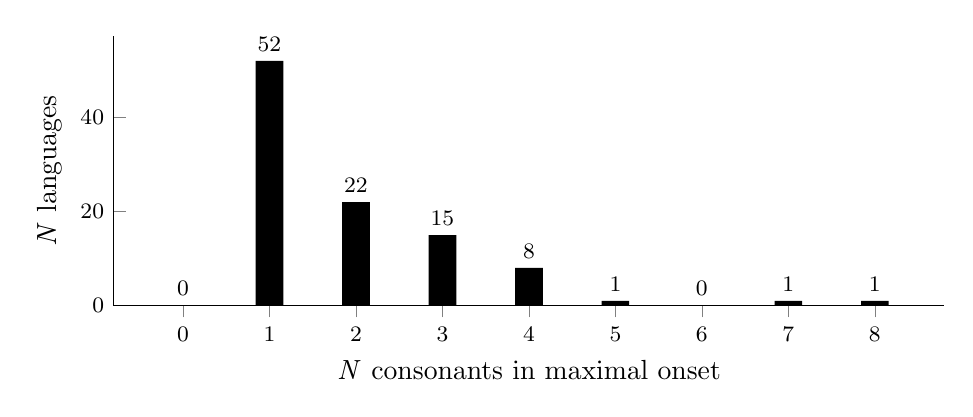
\begin{tikzpicture}
            \begin{axis}[
                    ybar,
                    ylabel={\textit{N} languages},
                    xlabel={\textit{N} consonants in maximal onset},
                    xtick=data,
                    axis lines*=left,
                    ymin=0,
                    scaled y ticks=false,
                    legend pos=north west,
                    ticklabel style={font=\footnotesize\scshape},
                    width=\textwidth,
                    height=5cm,
                    enlarge x limits={0.1},
                    nodes near coords,
                    nodes near coords style={text=black,font=\footnotesize},
                    ]
                \addplot+[
                     fill=black,draw=none
                    ] coordinates {(0,0) (1,52) (2,22) (3,15) (4,8) (5,1) (6,0) (7,1) (8,1)};
\end{axis}
\end{tikzpicture}
\caption{\label{fig:3.1}Maximal onset sizes in sample.}
\end{figure}


\begin{figure}
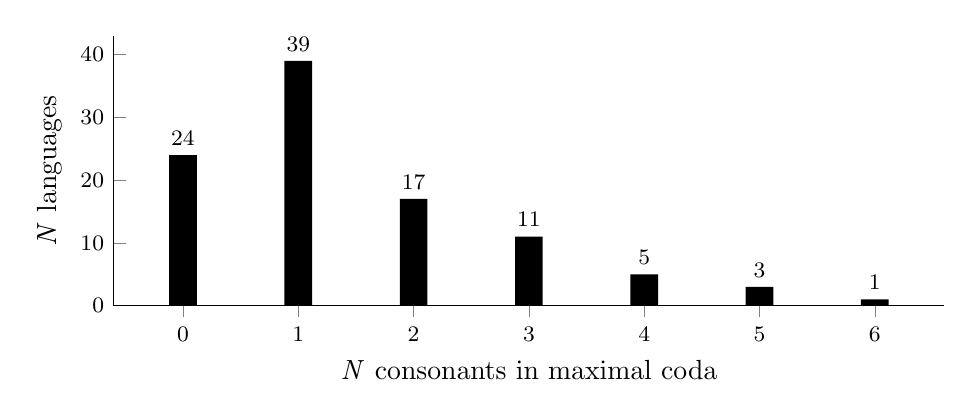
\begin{tikzpicture}
            \begin{axis}[
                    ybar,
                    ylabel={\textit{N} languages},
                    xlabel={\textit{N} consonants in maximal coda},
                    xtick=data,
                    axis lines*=left,
                    ymin=0,
                    scaled y ticks=false,
                    legend pos=north west,
                    ticklabel style={font=\footnotesize\scshape},
                    width=\textwidth,
                    height=5cm,
                    enlarge x limits={0.1},
                    nodes near coords,
                    nodes near coords style={text=black,font=\footnotesize},
                    ]
                \addplot+[
                     fill=black,draw=none
                    ] coordinates {(0,24) (1,39) (2,17) (3,11) (4,5) (5,3) (6,1)};
\end{axis}
\end{tikzpicture}
\caption{\label{fig:3.2}Maximal coda sizes in sample.}
\end{figure}

  The data presented in Figures \ref{fig:3.1} and \ref{fig:3.2} are for onset and coda patterns determined through the procedure described in \sectref{sec:3.2.1}. They do not include the largest word-marginal patterns which occur in languages with syllabic obstruents. There are four languages in the sample which are reported to have syllabic obstruents resulting in Highly Complex patterns at word margins.\footnote{{Additionally, Tohono O’odham has syllabic obstruents, but only in independent grammatical particles consisting of a single consonant (determiners and conjunctives). These are not reported to be phonologically bound to adjacent words. Therefore I do not include Tohono O’odham in \tabref{tab:3.1}.}} These patterns are presented in \tabref{tab:3.1}, along with the reported maximal onset and coda patterns in the languages.

\begin{table}
\begin{tabular}{lcccc}
\lsptoprule
           &                 &                & \multicolumn{2}{c}{Maximal obstruent string}\\\cmidrule(lr){4-5}
{Language} & {Maximal onset} & {Maximal coda} & word-initial & word-final\\\midrule
Cocopa & 4 & 3 & 5 & \phantom{>}3\\
Semai & 2 & 1 & 4 & \phantom{>}1\\
Tashlhiyt & 1 & 1 & \multicolumn{2}{r}{\textit{(words without vowels)}}\\
Tehuelche & 2 & 3 & 3 & >3\\
\lspbottomrule
\end{tabular}
\caption{\label{tab:3.1}Languages in Highly Complex category with syllabic obstruents. Maximal reported onsets and codas are given in first two columns. The sizes of the maximal word-marginal obstruent strings which occur as the result of syllabic obstruents are given in last two columns.}
\end{table}

  In Tashlhiyt, the size of maximal word-marginal obstruent strings cannot be determined, because there are many examples of words consisting entirely of obstruents in this language \REF{ex:3.12}. 

\ea\label{ex:3.12}
  \textbf{Tashlhiyt} (\textit{Afro-Asiatic}; Morocco)

\textit{tftktstː}

tf.tk.tstː\\
\glt ‘you took it off (\textsc{f})’
\citep[332]{Ridouane2008}
\z

In Tehuelche, the reference indicates that sequences of up to six consonants may occur word-finally, but the only illustrative example of a pattern this size is given is \REF{ex:3.13}.

\ea\label{ex:3.13}
\etriple{Tehuelche}{Chonan}{Argentina}

\textit{kt͡ʃaʔʃpʃk’n}

k.t͡ʃaʔʃp.ʃ.k’n\\
\glt ‘it is being washed’

(\citealt{FernándezGarayHernández2006}: 13)
\z

This example includes a nasal which may be syllabic (syllable peaks in CC syllables are not marked by the authors). It is clear from the language description that long obstruent sequences come about when syllabic consonants are strung together, but unclear as to what the upper limit on the size of these is. Word-final sequences of at least four obstruents are attested \REF{ex:3.14}.

\ea\label{ex:3.14}
\etriple{Tehuelche}{Chonan}{Argentina}

\textit{maːleʃpʃk’}

maː.leʃp.ʃ.k’\\
\glt ‘they steal’

(\citealt{FernándezGarayHernández2006}: 63)
\z

\subsection{Relationship between onset and coda complexity}\label{sec:3.3.2}

  Here I present an analysis similar to the one presented in \sectref{sec:2.2} for the Complex portion of the \citet{Maddieson2013a} sample. The languages of the sample used in this book are distributed according to their maximal onset and coda patterns.

\begin{table}
\begin{tabular}{l*{2}{r}*{6}{c}}
\lsptoprule
\multicolumn{1}{p{2.25cm}}{Number of Cs\newline in coda} & \multicolumn{8}{c}{Number of Cs in onset}\\\cmidrule(lr){2-9}
 & {One} & {Two} & {Three} & {Four} & {Five} & {Six} & {Seven} & {Eight}\\\midrule
None & 20 & 1 & 2 & 1 & -- & -- & -- & --\\
One & 21 & 12 & 5 & 1 & -- & -- & -- & --\\
Two & 7 & 5 & 5 & -- & -- & -- & -- & --\\
Three & 1 & 4 & 2 & 4 & -- & -- & -- & --\\
Four & 3 & -- & -- & 2 & -- & -- & -- & --\\
Five & -- & -- & -- & -- & 1 & -- & 1 & 1\\
Six & -- & -- & 1 & -- & -- & -- & -- & --\\
\lspbottomrule
\end{tabular}
\caption{\label{tab:3.2}Languages of sample distributed according to maximal onset and coda size.}
\end{table}

  Interestingly, it is common for languages with large clusters at one syllable margin to also exhibit large clusters at the other syllable margin in their canonical patterns. Roughly half of languages in the sample which have a maximal cluster of four or more consonants at one syllable margin will have a similarly large maximal cluster at the other syllable margin. It is striking that \textit{all} languages in the sample with maximal onsets of five or more consonants (Georgian, Itelmen, and Polish) also have maximal codas of five consonants. Meanwhile, the bottom left and top right corners of \tabref{tab:3.2} are sparsely populated; that is, there are relatively few languages with very large maximal clusters at one syllable margin and very small maximal clusters (or none at all) at the other margin. A similar pattern can be observed in \tabref{tab:2.2} in \sectref{sec:2.2}, which used a larger sample of 147 languages. Speaking from a strictly distributional point of view, there is no obvious motivation for this pattern. If we consider onset and coda structures to be independent structures, then we would expect to see the full range of possible variation in their combination crosslinguistically. This point will be revisited in \sectref{sec:3.5} and again in \chapref{sec:8}.

\subsection{Syllable structure complexity and obligatoriness of syllable margins}\label{sec:3.3.3}

  \citet[336]{Blevins2006} notes another crosslinguistic pattern linking onset and coda structures: she observes that languages with only open syllables tend to have optional onsets. In \tabref{tab:3.3} I examine this relationship in the current language sample. There are some languages in which optional onsets may be reported for the canonical syllable structure, but regular and obligatory consonant epenthesis (usually of a glottal stop or fricative) occurs to produce onsets in all ‘surface’ forms. In the analysis below, I consider such languages as having obligatory onsets.

\begin{table}
\begin{tabular}{ccc}
\lsptoprule
 \textit{N} languages & Codas occur? & Onset obligatory?\\\midrule
 14 & Y & Y\\
 62 & Y & N\\
 \phantom{1}2 & N & Y\\
 22 & N & N\\
\lspbottomrule
\end{tabular}
\caption{\label{tab:3.3}Languages in sample distributed according to occurrence of codas and obligatoriness of onsets.}
\end{table}

  The relationship reported by Blevins is upheld in the current sample. Of the 24 languages with only open syllables (no codas), only two are reported to have obligatory onsets. Obligatory onsets are more common in languages with coda structures (14/76). The two languages in the sample with obligatory onsets and only open syllables are Hadza (Simple) and Yine (Highly Complex). It should also be noted that the Oykangand dialect of Kunjen used here is reported to have obligatory codas. Kunjen is argued to have very marginal onset patterns, with onsets occurring in interjections and sentence-initially in a just a few lexical items (\citealt{Sommer1969,Sommer1970,Sommer1981}, though see \citealt{Dixon1970} for an opposing view).\footnote{{According to Sommer’s analysis, Kunjen is a rare example of a language without phonological CV syllables. Another language argued not to have phonological CV syllables is Arrernte, a Pama-Nyungan language of central Australia (cf. \citealt{BreenPensalfini1999}), though \citet{Anderson2000} reports a canonical surface syllable structure of (C)(C)V(C) for Western Arrernte.}} Therefore Kunjen shows a very similar pattern to Hadza and Yine, except that the syllable margins are reversed.

  The analysis above motivated a more general examination of obligatory syllable margin patterns in the language sample with respect to syllable structure complexity (\tabref{tab:3.4}).

\begin{table}
\begin{tabular}{l *{4}{>{\itshape}c}}
\lsptoprule
& \multicolumn{4}{c}{Syllable structure complexity}\\\cmidrule(lr){2-5}
& \normalfont S & \normalfont MC & \normalfont C & \normalfont HC\\
& \normalfont \textit{N} = 24 & \normalfont \textit{N} = 26 & \normalfont \textit{N} = 25 & \normalfont \textit{N} = 25\\\midrule
{Onset obligatory} & Hadza        & Kambaata   &  Koho   &  Bench   \\
                   & Ute          &    Karok           &      Lepcha       &      Nuu-chah-nulth\\
                   & \normalfont (2)          &       Lao          &      Mangarrayi   &           Semai\\
                   &              &    Pacoh           &    \normalfont(3)            &       Thompson\\
                   &              &   \normalfont (4)              &                   &       Tohono O’odham\\
                   &              &                    &                   &        Yakima Sahaptin\\
                   &              &                    &                   &         Yine\\
                   &              &                    &                   &         \normalfont(7)\\
{Coda obligatory}  & -- & -- & -- & Kunjen \\
                   &   &   &   & \normalfont (1)\\
\lspbottomrule
\end{tabular}
\caption{\label{tab:3.4}Languages in sample with obligatory syllable margins.}
\end{table}

  Obligatory syllable margins are a minor pattern in the language sample, occurring in only 17 languages, but this feature is most common in languages with Highly Complex syllable structure, occurring in roughly one-third (8/25) of those languages. This feature is least common in languages with Simple syllable structure (2/24 languages). The pattern in the Highly Complex category is statistically significant when compared against the patterns in the other three categories combined (p = .03 in Fisher’s exact test). This association between syllable structure complexity and obligatoriness of syllable margins has, to my knowledge, not been previously reported.

  Obligatory syllable margins are more common in some areas than others: Five of the languages in \tabref{tab:3.4} are from Southeast Asia \& Oceania. North America is also heavily represented, accounting for another six languages altogether, including four of the languages with obligatory syllable margins from the Highly Complex group. It should further be noted that most of the North American languages with obligatory syllable margins in the Highly Complex group are from the Pacific Northwest (Nuu-chah-nulth, Thompson, and Yakima Sahaptin), so areal factors may be at play. Nevertheless, the Highly Complex pattern in \tabref{tab:3.4} is not entirely areal in nature, as it includes languages from Africa, Southeast Asia \& Oceania, South America, and Australia \& New Guinea. 

  Interestingly, the description of Itelmen (Chukotko-Kamchatkan, Highly Complex) suggests that this language, too, had obligatory onsets at some point in its history: morphophonological processes suggest that present-day vowel-initial syllables were at one time initiated by a glottal stop (\citealt{GeorgVolodin1999}: 48).

\subsection{Vocalic nucleus patterns}\label{sec:3.3.4}

  Vocalic nucleus patterns have until now been excluded from the discussion of syllable patterns, as they are not considered in the definitions of syllable structure complexity used here. However, it is important to note that vocalic nucleus patterns can also exhibit different degrees of complexity. In \tabref{tab:3.5} I present a very general analysis of these patterns in the sample, showing the distribution of simple and complex vocalic nuclei by syllable structure complexity.

\begin{table}
\begin{tabular}{lcccc}
\lsptoprule
 & \multicolumn{4}{c}{Syllable Structure Complexity}\\\cmidrule(lr){2-5}
  & S & MC & C & HC\\
  Languages with:     & \textit{N} = 24 & \textit{N} = 26 & \textit{N} = 25 & \textit{N} = 25\\\midrule
 Simple vocalic nuclei only & 12 & \phantom{1}9 & \phantom{1}9 & \phantom{1}9\\
 Complex vocalic nuclei\footnote{\textit{(long vowels, diphthongs, and\slash or vowel sequences)}} & 12 & 17 & 16 & 16\\
\lspbottomrule
\end{tabular}
\caption{\label{tab:3.5}Vocalic nucleus patterns in language sample, by syllable structure complexity.}
\end{table}

  Simple vocalic nuclei -- those consisting of a single short vowel -- occur in every language. The first row of \tabref{tab:3.5} shows the number of languages in each complexity category for which this is the only vocalic nucleus pattern occurring. Languages in which complex vocalic nuclei occur in addition to simple vocalic nuclei are shown in the second row. For the sake of simplicity I have collapsed three different kind of complex vocalic nucleus patterns in the analysis here. A language is counted as having long vowels if it has contrastive vowel length, but not if it has predictable vowel lengthening, e.g., a longer variant preceding a voiced coda. Diphthongs and tautosyllabic vowel sequences are difficult to disambiguate from one another, as their analyses by different authors may vary widely; however, vowel sequences reported here as syllable nuclei are those explicitly shown by the author to belong to one syllable, much like a diphthong. That is, this figure does not include cases of hiatus, in which the two vowels in a sequence belong to different syllables.

  \tabref{tab:3.5} shows that complex vocalic nuclei are much less likely to occur in languages with Simple syllable structure than in languages from the other categories. This suggests that the potential for more syllable types in languages with more complex syllable structure may be not only a function of larger canonical syllable margins, but also of greater diversity in syllable nucleus patterns. Nevertheless, the analysis above is too coarse to draw strong conclusions about vocalic nucleus patterns and syllable structure complexity. The issue of contrastive vowel length will be treated in greater detail in \chapref{sec:4}, along with contrastive nasalization, voicing, and glottalization patterns in the vowel inventories of the sample.

\subsection{Syllabic consonants}\label{sec:3.3.5}

  In this section I investigate patterns of syllabic consonants in the data. Recall that the previous literature suggests two competing predictions for the relationship between syllable complexity and the presence of syllabic consonants. \citegen{Isačenko1939/1940} phonological typology predicts that ‘vocalic’ languages, which tend to have simpler syllable structure, will be more likely to develop syllabic consonants, and specifically syllabic sonorants. Meanwhile, \citet{Bell1978a} notes that syllabic consonants, including syllabic obstruents, often come about through vowel reduction processes, which are also known to produce the clusters characteristic of languages with more complex syllable structure. On the basis of the latter observation, in \sectref{sec:3.1.2} I formulated a hypothesis that languages with more complex syllable structure are more likely to have syllabic consonant patterns.

  Here I analyze languages in which the syllabic consonants are reported as invariant patterns. Most often, the syllabicity of these consonants is predictable from the surrounding consonantal and/or word environment, as illustrated by \REF{ex:3.15}. Less frequently, syllabic consonants are analyzed as separate phonemes which are contrastive with their non-syllabic counterparts (\ref{ex:3.16}a--b).

\ea\label{ex:3.15}
  \textbf{Itelmen} (\textit{Chukotko-Kamchatkan}; Russia)

\textit{A word-initial alveolar or bilabial nasal stop preceding another consonant is realized as syllabic.}

/\textbf{m}ɬim/

[\textbf{m̩}ɬim]\\
\glt ‘blood’

(\citealt{GeorgVolodin1999}: 16)
\z

\ea\label{ex:3.16}
  \textbf{Ewe} (\textit{Atlantic-Congo}; Ghana, Togo)
\ea   jɔm̩̀
\glt  ‘call me’
\ex kampé
\glt  ‘scissors’
\citep[38]{Ameka1991}
\z
\z

  Three languages are excluded from the current analysis: Chipaya, Nimboran (both from the Complex category), and Yine (from the Highly Complex category). For all three of these languages, there are conflicting reports regarding the occurrence of syllabic consonants, sometimes from the same author.\footnote{{There are a few other languages for which there are suggestions of alternate analyses. The dialect of Sahaptin analyzed here, Yakima, is argued not to have syllabic consonants by \citet{HargusBeavert2006} on the basis of distributional and phonological behavior of consonants in sequences. However, it should be noted that \citet{Minthorn2005} argues for syllabic consonants, including obstruents, in the closely related dialect of Umatilla Sahaptin, on the basis of speaker intuition and acoustic analysis. Additionally, one description of Alamblak lists an example of a word consisting entirely of obstruents:} \textrm{\textit{kpt}} \textrm{‘basket type’ \citet[1]{EdmistonEdmiston2003}; however, no further elaboration is given and obstruents are not included in the description of syllabic consonants in \citet{Bruce1984}, so it is unclear whether syllabic obstruents are an issue of debate for this language. Finally, for Itelmen, \citet[42]{Volodin1976} gives transcriptions of lexical items consisting entirely of obstruents (}\textrm{\textit{t͡ʃkpt͡ʃ} }\textrm{‘spoon’). In a later reference, he describes only syllabic sonorants in the language (\citealt{GeorgVolodin1999}).}} For example, Matteson gives the following description for Yine, which seems to suggest that consonants in complex onsets both belong to a syllable with a vocalic nucleus and are simultaneously themselves syllabic:

\begin{quote}
“We number the consonants of the syllable, beginning with the consonant that immediately precedes the nuclear vowel: +C\textsuperscript{3} +C\textsuperscript{2} +C\textsuperscript{1}V. In the positions of consonants C\textsuperscript{2} and C\textsuperscript{3} occur syllabic allophones of the consonants. Thus the syllable is a complex unit consisting of from one to three syllabic units.” 
\citep[23]{Matteson1965}
\end{quote}

Because of the conflicting descriptions of these languages, I opted to exclude them from the current analysis. Georgian and Tashlhiyt also have conflicting descriptions with respect to the occurrence of syllabic consonants, but in both of these cases experimental evidence has been presented to support one analysis over another. The articulatory and acoustic experiments in \citet{Ridouane2008} and \citet{GoldsteinEtAl2007} support a syllabic consonant analysis for Tashlhiyt, while native speaker intuition reported in \citet{Chitoran1999} does not support an analysis of syllabic sonorants for Georgian. It is interesting to note that all of the languages with conflicting descriptions -- those discussed here and the ones mentioned in the footnote -- are from the Complex and Highly Complex categories. This recalls the observation noted previously, in which transitions in consonant clusters on the one hand and syllabic consonants on the other may have similar motivations and acoustic manifestations.

\begin{table}
\begin{tabular}{lcccc}
\lsptoprule
 & \multicolumn{4}{c}{Syllable Structure Complexity}\\\cmidrule(lr){2-5}
                        & S & MC & C & HC\\
  Languages with:       &  \textit{N} = 24   & \textit{N} = 26                & \textit{N} = 23     & \textit{N} = 24\\\midrule

 Syllabic consonants\\
   of any kind                         & \textbf{2} & \textbf{6} & \textbf{5} & \textbf{11}\\
 \textit{Syllabic nasals} & 2 & 5 & 5 & 10\\
 \textit{Syllabic liquids} & -- & 2 & 1 & 6\\
 \textit{Syllabic obstruents} & -- & -- & -- & 5\\
 No syllabic\\
    consonants            & \textbf{22} & \textbf{20} & \textbf{18} & \textbf{13}\\
\lspbottomrule
\end{tabular}
\caption{\label{tab:3.6}Presence of invariant syllabic consonants in language sample, by syllable structure complexity. Chipaya, Nimboran (Complex) and Yine (Highly Complex) excluded.}
\end{table}

  The syllabic consonant patterns reported for the languages of the sample can be found in \tabref{tab:3.6}. There is a steadily increasing trend in the proportion of languages with these patterns as syllable structure complexity increases: only two of languages with Simple syllable structure are reported to have syllabic consonants, compared to 11 of the languages in the Highly Complex category. The trend in the Highly Complex category is statistically significant when compared to the trends in the other three categories combined (p = .01 in Fisher’s exact test). Examining the particular kinds of syllabic consonants represented, the patterns are similar to what is reported in \citet{Bell1978a}. Most languages with syllabic consonants have syllabic nasals, and languages with syllabic obstruents are rare. While languages from all four categories have syllabic nasals and most have syllabic liquids, syllabic obstruents are only reported for languages in the Highly Complex category. This is not a remnant of the way the Highly Complex category is defined: recall that languages with syllabic obstruents are categorized as Highly Complex only if these structures participate in word-marginal sequences of three obstruents or more. It is striking that no languages with simpler syllable structure are reported to have syllabic obstruents. Even if the three languages excluded from the previous analysis were included here, the distribution of syllabic obstruents would be among two languages with Complex syllable structure and six languages with Highly Complex syllable structure. 

  It should also be noted that three of the languages with syllabic obstruents (Cocopa, Semai, Tashlhiyt) are reported to also have both syllabic nasals and syllabic liquids. Tehuelche does not have syllabic liquids. Tohono O’odham is the only language which has syllabic obstruents but not syllabic sonorant consonants. This indicates that the trend in \tabref{tab:3.6} -- by which Highly Complex languages are more likely than any of the other categories to have syllabic consonants  -- is not driven by the inclusion of syllabic obstruents in the definition of that category, or skewed by potential misanalyses which confound syllabic obstruents and large tautosyllabic clusters. Instead, the trend can be obtained from the syllabic nasal and liquid patterns in the sample.

  While the analyses presented above are for the invariant syllabic consonant patterns observed in the sample, there were also several cases in which syllabic consonants were reported to occur in variation with CV or VC sequences, as illustrated by \xxref{ex:3.17}{ex:3.18}.

\ea\label{ex:3.17}
\etriple{Sichuan} \textbf{Yi}{Sino-Tibetan}{China}

\textit{Nasals and laterals preceding [ɨ] occur in free variation with syllabic consonants.}

/lɨ/

[lɨ]{\textasciitilde}[\textbf{l̩}]
\citep[31]{Gerner2013}
\z

\ea\label{ex:3.18}
   \textbf{Mamaindê} (\textit{Nambiquaran}, Brazil)

\textit{When an unstressed vowel is lost resulting in a sequence of nasal plus consonant, a preceding nasal becomes syllabic.}

/ˈjohnalatʰawa/

[ˈjoh\textbf{n̩}latʰwa]\\
\glt ‘it is low’
\citep[262-3]{Eberhard2009}
\z

\begin{table}
\begin{tabular}{lcccc}
\lsptoprule
 & \multicolumn{4}{c}{Syllable Structure Complexity}\\\cmidrule(lr){2-5}
 Languages with  & S & MC & C & HC\\
   variable:     &   \textit{N} = 1 & \textit{N} = 3 &  \textit{N} = 2 & \textit{N} = 3\\\midrule
 \textit{Syllabic nasals}     & 1 & 3 & 2 & 3\\
 \textit{Syllabic liquids}    & 1 & -- & -- & 2\\
 \textit{Syllabic obstruents} & -- & 1 & -- & 1\\
\lspbottomrule
\end{tabular}
\caption{\label{tab:3.7}Distribution of languages in sample with syllabic nasals, liquids, and obstruents occurring in variation with VC or CV structures.}
\end{table}

  \tabref{tab:3.7} shows the distribution of variable processes producing syllabic consonants in the data. Though the data set is very small, it is interesting that the general distributional pattern is similar to that presented in \tabref{tab:3.6}. The occurrence of syllabic consonants in variation with VC or CV structures is least frequent among languages with Simple syllable structure, and in all categories nasals are the most common syllabic consonant to result. Variable syllabic obstruents occur in two languages. In Paiwan (Moderately Complex), syllabic obstruents may occur when schwa is reduced immediately after a sibilant in rapid speech, and in Kabardian (Highly Complex), they occur as the result of an optional process of high vowel contraction (\ref{ex:3.19}--\ref{ex:3.20}):

\ea\label{ex:3.19}
  \textbf{Paiwan} (\textit{Austronesian}; Taiwan)

/səkam/

[səkam]{\textasciitilde}[\textbf{s̩}kam]\\
\glt ‘mattress’
\citep[41]{Chang2006}
\z

\ea\label{ex:3.20}
  \textbf{Kabardian} (\textit{Abkhaz-Adyge}; Russia, Turkey)

/ɬ{}'əʒ/

[ɬ’iʒ]{\textasciitilde}[ɬ{}'\textbf{ʒ̩}]\\
\glt ‘old man’
\citep[24]{Kuipers1960}
\z

Kabardian is also the only language in the sample reported to have both invariant syllabic consonants (for sonorants in certain consonant environments) and variable syllabic consonants as a result of synchronic phonetic processes like the one illustrated above.

  Returning to the hypothesis stated at the beginning of this section, there is evidence that languages with more complex syllable structure are more likely to have syllabic consonant patterns. Specifically, languages with Highly Complex syllable structure are the most likely of all those in the sample to have invariant syllabic consonants, while languages with Simple syllable structure are the least likely. Variable processes resulting in syllabic consonants are also relatively more frequent in languages with non-Simple syllable structure.

\subsection{Morphological patterns}\label{sec:3.3.6}

  In this section I analyze the morphological patterns associated with syllable patterns in the language sample. First, I report the morphological constituency patterns observed in the maximal onset and coda structures in each language. Then I present an analysis of the kinds of morphemes (lexical or grammatical) in which syllabic consonants in the language sample occur. I test the hypotheses formulated in \sectref{sec:3.1.2} with respect to these patterns: first, that as syllable structure complexity increases, so does the likelihood that the largest syllable margin types in a language will be morphologically complex; second, that as syllable structure complexity increases, so does the likelihood that syllabic consonants occurring in a language will belong to grammatical elements.

  Since morphologically complex instances of syllable patterns are often not explicitly described and must be gathered from the examples, it was impractical and in many cases impossible to find morpheme-internal and morphologically complex instances of the same specific consonant sequence in each language, especially for the larger clusters. The patterns analyzed here are for the maximal onset and coda \textit{types}, e.g. CC. For example, the maximal coda in Gaam is two consonants. The word-final patterns shown in the examples below would be taken as evidence that the maximal coda occurs in both morpheme-internal (\ref{ex:3.21}a) and morphologically complex (\ref{ex:3.21}b) contexts.

\ea\label{ex:3.21}
\etriple{Gaam}{Eastern Jebel}{Sudan}

\ea  bāɡd̪à\textbf{rs}\\
\glt ‘lizard type’
\ex  ɡəū\textbf{r-d̪}\\
stomach-\textsc{sg}\\
\glt ‘stomach’
(\citealt{Stirtz2011}: 32, 37)
\z
\z

  Note also that the definition of \textit{morphologically complex} here refers to sequences derived by any morphological process. That is, sequences derived through reduplication or nonconcatenative processes such as subtractive morphology are also considered to be morphologically complex, even though they don’t involve more than one distinct morpheme.

  First I test \citegen{Greenberg19651978} prediction in the data: as the size of a syllable margin increases, so does the probability that it contains morpheme boundaries. Figures \ref{fig:3.3} and \ref{fig:3.4} show morphological constituency patterns in maximal onset and coda types in the data.

  
\begin{figure}
\begin{tikzpicture}
\pgfplotstableread{data/fig33.csv}{\table}
    \pgfplotstablegetcolsof{\table}
    \pgfmathtruncatemacro\numberofcols{\pgfplotsretval-1}
            \begin{axis}[easterdaystacked,
                                xticklabels={CC,CCC,CCCC,{CCCCC or more}},
                        ]
            \foreach \i in {1,...,\numberofcols} {
                \addplot+[
                    /pgf/number format/read comma as period, fill
                    ] table [x index={1},y index={\i},x expr=\coordindex] {\table};
                \pgfplotstablegetcolumnnamebyindex{\i}\of{\table}\to{\colname} % Adding column headers to legend
                \addlegendentryexpanded{\colname}
            }
            \end{axis}                                                                           
\end{tikzpicture}
\caption{\label{fig:3.3}Morphological constituency patterns in maximal onset types in data. For each maximal onset type, figure shows proportion of languages exhibiting the given morphological patterns for that type.}
\end{figure}


\begin{figure}
\begin{tikzpicture}
\pgfplotstableread{data/fig34.csv}{\table}
    \pgfplotstablegetcolsof{\table}
    \pgfmathtruncatemacro\numberofcols{\pgfplotsretval-1}
            \begin{axis}[easterdaystacked,
                                xticklabels={CC,CCC,CCCC,{CCCCC or more}},
                        ]
            \foreach \i in {1,...,\numberofcols} {
                \addplot+[
                    /pgf/number format/read comma as period, fill
                    ] table [x index={1},y index={\i},x expr=\coordindex] {\table};
                \pgfplotstablegetcolumnnamebyindex{\i}\of{\table}\to{\colname} % Adding column headers to legend
                \addlegendentryexpanded{\colname}
            }
            \end{axis}                                                                           
\end{tikzpicture}
\caption{\label{fig:3.4}Morphological constituency patterns in maximal coda types in data. For each maximal coda type, figure shows proportion of languages exhibiting the given morphological patterns for that type.}
\end{figure}

  For both maximal onset and maximal coda patterns in the data, the proportion of languages having these clusters solely in morphologically complex contexts increases with cluster size. However, morphologically complex patterns also occur alongside morpheme-internal patterns in the maximal margins for a number of languages (the “Both patterns” trend in Figures \ref{fig:3.3} and \ref{fig:3.4}). When this trend is additionally considered, we find that maximal coda cluster types are generally more likely than maximal onset types to exhibit morphologically complex patterns. We also find that all maximal cluster types of five consonants or larger are found only in morphologically complex contexts.

  Interestingly, there are some language-internal patterns in the data which go against Greenberg’s prediction. In Lelepa there are biconsonantal onsets showing both morphological patterns, but the only attested triconsonantal onsets are within morphemes (\ref{ex:3.22}a-c).

\ea\label{ex:3.22}
\etriple{Lelepa}{Austronesian}{Vanuatu}

\ea  n-maloɡo\\
\textsc{nmlz}-darken\\
\glt ‘darkness’

\ex  nmal\\
\glt ‘trunk’

\ex  psruki\\
\glt ‘speak’

(\citealt{Lacrampe2014}: 107, 207, 42)
\z
\z

  The analyses presented in Figures \ref{fig:3.3}--\ref{fig:3.4} test Greenberg’s specific predictions regarding cluster size. However, the hypothesis in (\ref{ex:3.4}a) is formulated with respect to syllable structure complexity, which is a slightly different question, though we expect to find a similar pattern due to how the categories are defined. In Figures \ref{fig:3.5}--\ref{fig:3.6} I present the morphological constituency patterns observed by syllable structure complexity category. Note that these figures only include the languages from each category which have complex onsets or complex codas, respectively.


\begin{figure}
\begin{tikzpicture}
\pgfplotstableread{data/fig35.csv}{\table}
    \pgfplotstablegetcolsof{\table}
    \pgfmathtruncatemacro\numberofcols{\pgfplotsretval-1}
            \begin{axis}[easterdaystacked,
                                xticklabels={{MC}, C, {HC}},
                        ]
            \foreach \i in {1,...,\numberofcols} {
                \addplot+[
                    /pgf/number format/read comma as period, fill
                    ] table [x index={1},y index={\i},x expr=\coordindex] {\table};
                \pgfplotstablegetcolumnnamebyindex{\i}\of{\table}\to{\colname} % Adding column headers to legend
                \addlegendentryexpanded{\colname}
            }
            \end{axis}                                                                           
\end{tikzpicture}
\caption{\label{fig:3.5}Morphological constituency patterns in maximal complex onsets, by syllable structure complexity category. For each category, the figure shows the proportion of languages exhibiting the given morphological patterns in its complex onsets.}
\end{figure}


\begin{figure}
\begin{tikzpicture}
\pgfplotstableread{data/fig36.csv}{\table}
    \pgfplotstablegetcolsof{\table}
    \pgfmathtruncatemacro\numberofcols{\pgfplotsretval-1}
            \begin{axis}[easterdaystacked,
                                xticklabels={C, {HC}},
                        ]
            \foreach \i in {1,...,\numberofcols} {
                \addplot+[
                    /pgf/number format/read comma as period, fill
                    ] table [x index={1},y index={\i},x expr=\coordindex] {\table};
                \pgfplotstablegetcolumnnamebyindex{\i}\of{\table}\to{\colname} % Adding column headers to legend
                \addlegendentryexpanded{\colname}
            }
            \end{axis}                                                                           
\end{tikzpicture}
\caption{\label{fig:3.6} Morphological constituency patterns in maximal complex codas, by syllable structure complexity category. For each category, the figure shows the proportion of languages exhibiting the given morphological patterns in its complex onsets. Note that the one language with complex codas from the Moderately Complex category -- Eastern Khanty -- is not included in the figure. Its very marginal complex codas are always morphologically complex.}
\end{figure}


  The figures show that as syllable structure complexity increases, both maximal onset and maximal coda clusters are more likely to have morphologically complex patterns, confirming the hypothesis in (\ref{ex:3.4}a).

  The patterns in Figures~\ref{fig:3.5}--\ref{fig:3.6} are combined in \figref{fig:3.7} in order to show the general trend for morphologically complex patterns in maximal syllable-mar\-gin\-al clusters with respect to syllable structure complexity in the language sample. In this figure onset and coda patterns are collapsed, and the “both contexts” and “only morphologically complex” patterns are combined. For each category, the figure shows the percentage of languages with complex syllable margins for which morphologically complex patterns occur in either or both maximal syllable margins.


\begin{figure}  
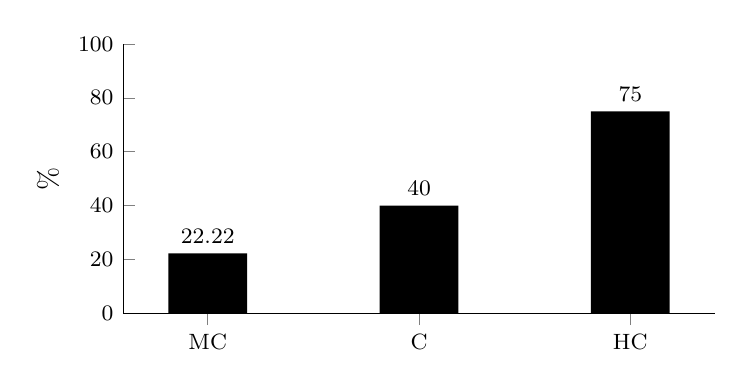
\begin{tikzpicture}
            \begin{axis}[
                    ybar,
                    ylabel={\%},
                    xtick=data,
                    axis lines*=left,
                    ymin=0,
                    ymax=100,
                    legend pos=north west,
                    ticklabel style={font=\footnotesize},
                    width=.75\textwidth,
                    enlarge x limits={.2},
                    height=5cm,
                    bar width=1cm,
                    nodes near coords,
                    nodes near coords style={text=black,font=\footnotesize},
                    xticklabels={{MC}, C, {HC}},
                    ]
                \addplot+[
                     fill=black,draw=none
                    ] coordinates {(0,22.2222222222222) (1,40) (2,75)};
\end{axis}
\end{tikzpicture}
\caption{\label{fig:3.7} Percentage of languages in each category exhibiting morphologically complex patterns in either or both of its maximal syllable margins.}
\end{figure}

  Morphologically complex patterns can be found in the maximal syllable margins of most languages from the Highly Complex category, and this pattern is statistically significant when compared against the patterns in the other two categories combined (p < .01 in Fisher’s exact test). However, there are six languages in this category for which I could determine only morpheme-internal patterns. In Wutung, the maximal margin is explicitly described as occurring within a few apparently single-morpheme lexical items. In Kunjen and Lezgian, maximal coda and onset clusters, respectively, seem to be limited to single-morpheme lexical items, though the references consulted do not explicitly state this. In Menya, the only morphologically complex instance of a maximal cluster that could be found was in an abstract phonemic transcription for which the phonetic form was unclear. In Passamaquoddy-Maliseet, examples of morphologically complex instances of maximal clusters could not be found, though it seems as though the morphology could produce them. The remaining language, Semai, has syllabic consonants and will be discussed below.

  Recall that there are four languages in the Highly Complex portion of the sample for which the largest word-marginal obstruent sequences include syllabic consonants. The maximal ‘true’ onset/coda clusters reported for these languages (cf. \tabref{tab:3.2}) were included in the previous analyses in this section, but the maximal word-marginal sequences were not. I present the morphological patterns for these sequences in \tabref{tab:3.8}.

\begin{table}
\begin{tabular}{lcccc}
\lsptoprule
{Language}& {Maximal \#\_} & {Morphol.} & Maximal \_\#  & Morphol. \\
          &   obstruent string     &      pattern                   &  obstruent string   &      pattern                \\\midrule
Cocopa    & 5                      & complex & 3                      & complex\\
Semai     & 4                      & complex & 1                      & --\\
Tashlhiyt & --\footnote{(words without vowels)} & complex & --\textsuperscript{\itshape a} & complex\\
Tehuelche & 3                      & complex & >3                     & complex\\
\lspbottomrule
\end{tabular}
\caption{\label{tab:3.8}Morphological patterns of maximal word-marginal obstruent sequences in languages with syllabic obstruents in Highly Complex category.}
\end{table}

  All of the maximal word-marginal obstruent sequences in the languages in \tabref{tab:3.8} occur in morphologically complex contexts. For example, in Semai, all maximal word-initial consonant sequences, and indeed all word-initial sequences of more than two consonants, are derived through reduplication processes \REF{ex:3.23}.

\ea\label{ex:3.23}
  \textbf{Semai} (\textit{Austroasiatic}; Malaysia)

ɡp.ɡ.hup (< ɡhup )\\
\glt ‘irritation on skin (e.g., from bamboo hair)’

(\citealt{Sloan1988}: 320; \citealt{Diffloth1976a}: 256)
\z

Though maximal word-marginal obstruent string length cannot be determined in Tashlhiyt due to the occurrence of many words consisting entirely of obstruents in this language, the longest such words are morphologically complex \REF{ex:3.24}.

\ea\label{ex:3.24}
  \textbf{Tashlhiyt} (\textit{Afro-Asiatic}; Morocco)

t-sː-kʃf-t=stː

ts.sk.ʃf.tstː\\
\glt ‘you dried it (\textsc{f})’

(\citealt{Ridouane2008}: 332; interlinear gloss not provided)
\z

  Now we turn to the hypothesis in (\ref{ex:3.4}b): as syllable structure complexity increases, so does the likelihood that syllabic consonants occurring in a language will belong to grammatical elements. This is based partly on \citegen{Bell1978a} observation that the syllabic consonants in his typological survey were often restricted to grammatical particles and affixes.

  Only the languages reported in \sectref{sec:3.3.5} as having invariant syllabic consonant patterns are included in the analysis here. Additionally, Kabardian is excluded from the present analysis because its precise patterns could not be determined. For each kind of syllabic consonant analyzed (nasal, liquid, and obstruent), I determine whether that type occurs in lexical morphemes, grammatical morphemes, or both. For example, in Bench, syllabic nasals can be found in both lexical and grammatical morphemes \REF{ex:3.25}.

\ea\label{ex:3.25}
  \textbf{Bench} (\textit{Ta-Ne-Omotic}; Ethiopia)

\ea   ɡȕp\textbf{m\={} }\\
\glt ‘foam’

\ex   njāʔ-\textbf{n\={} }d

child-\textsc{pl}\\
\glt ‘children’

(\citealt{Rapold2006}: 107, 111)
\z
\z

  In Tables \ref{tab:3.9}--\ref{tab:3.11} I present analyses for the morphological patterns of each kind of syllabic consonant (nasal, liquid, and obstruent) observed in the data.

\begin{table}
\begin{tabular}{lcccc}
\lsptoprule
 & \multicolumn{4}{c}{Syllable structure complexity}\\\cmidrule(lr){2-5}
Languages with & S & MC & C & HC\\
syllabic nasals in: & \textit{N} = 2 & \textit{N} = 5 & \textit{N} = 6 & \textit{N} = 9\\\midrule
 \textit{Lexical morphemes only} & 1 & 3 & 2 & 1\\
 \textit{Lex. and gram. morphemes} & -- & 2 & 2 & 6\\
 \textit{Grammatical} \\
\textit{morphemes only} & 1 & -- & 2 & 2\\
\lspbottomrule
\end{tabular}
\caption{\label{tab:3.9}Morphological patterns of syllabic nasals in sample, by syllable structure complexity. Kabardian (Highly Complex) is omitted as its pattern could not be determined.}
\end{table}




\begin{table}
\begin{tabular}{lcccc}
\lsptoprule
 & \multicolumn{4}{c}{Syllable structure complexity}\\\cmidrule(lr){2-5}
Languages with & S & MC & C & HC\\
syllabic liquids in: & \textit{N} = 0 & \textit{N} = 2 & \textit{N} = 1 & \textit{N} = 5\\\midrule
 \textit{Lexical morphemes only} & -- & 2 & 1 & 2\\
 \textit{Lex. and gram. morphemes} & -- & -- & -- & 2\\
 \textit{Grammatical} \\
\textit{morphemes only} & -- & -- & -- & 1\\
\lspbottomrule
\end{tabular}
\caption{\label{tab:3.10}Morphological patterns of syllabic liquids in sample, by syllable structure complexity. Kabardian (Highly Complex) is omitted as its pattern could not be determined.}
\end{table}


\begin{table}
\begin{tabular}{lcccc}
\lsptoprule
 & \multicolumn{4}{c}{Syllable structure complexity}\\\cmidrule(lr){2-5}
Languages with & S & MC & C & HC\\
syllabic obstruents in: & \textit{N} = 0 & \textit{N} = 0 & \textit{N} = 0 & \textit{N} = 5\\\midrule
 \textit{Lexical morphemes only} & -- & -- & -- & --\\
 \textit{Lex. and gram. morphemes} & -- & -- & -- & 1\\
 \textit{Grammatical} \\
\textit{morphemes only} & -- & -- & -- & 4\\
\lspbottomrule
\end{tabular}
\caption{\label{tab:3.11}Morphological patterns of syllabic obstruents in sample, by syllable structure complexity.}
\end{table}

  In general, the pattern by which syllabic consonants are found to occur in grammatical morphemes, either exclusively or in addition to lexical morphemes, is the dominant one in the data. This is the case for 15/22 languages with syllabic nasals and all of the languages with syllabic obstruents. And within this very small data set, this trend also appears to increase with syllable structure complexity, suggesting support for the hypothesis. 

  In fact most of the languages with syllabic consonants in the Highly Complex category have these sounds in grammatical items. In Tehuelche, for example, \textit{all} syllabic consonants correspond to or belong to grammatical morphemes \REF{ex:3.26}.

\ea\label{ex:3.26}
\etriple{Tehuelche}{Chonan}{Argentina}

k.t͡ʃaʔʃp.ʃ.k’n

k-t͡ʃaʔʃp-ʃ-k’n

\textsc{refl}-wash-\textsc{ps-realis}\\
\glt ‘it is being washed’

(\citealt{FernándezGarayHernández2006}: 13)
\z

  To summarize, in this section the morphological patterns of maximal onset types, maximal coda types, and syllabic consonant inventories in the sample have been examined. In both cases there is support for the hypotheses in \REF{ex:3.4}. Clearly morphology contributes an important role to the development of complex syllable patterns. While this point will be only briefly revisited in the discussion in \sectref{sec:3.5}, it will be discussed in further detail in \chapref{sec:8}.

\section{Properties of highly complex syllable structure}\label{sec:3.4}

  Having described the general patterns of maximal onsets, maximal codas, and syllabic consonants in the data, I now turn to an examination of the properties of syllable structure in the languages in the Highly Complex portion of the sample. In \sectref{sec:3.4.1} I give examples of the syllable patterns occurring in each of these languages. In \sectref{sec:3.4.2} I attempt to characterize the prevalence of Highly Complex structures within each of the languages by examining restrictions on consonant combinations and reported frequency patterns. In \sectref{sec:3.4.3} I present information on the acoustic and perceptual properties of Highly Complex structures.

\subsection{Examples of Highly Complex syllable patterns in sample}\label{sec:3.4.1}

  In order to provide a better picture of what specific syllable patterns occur in the languages of the Highly Complex portion of the sample, I list some representative structures in \tabref{tab:3.12}. The definition of Highly Complex syllable structure includes any onset or coda structure of three obstruents, or of four consonants or more in length. It also includes any word-marginal sequence containing syllabic obstruents such that a sequence of three or more obstruents occurs at a word margin. For each language I give a set of examples for each onset, coda, and/or word-marginal cluster that occurs at each of the following lengths: three consonants, four consonants, and five or more consonants. For Tashlhiyt, I have given some examples of vowelless words in the rightmost column, but have not assigned them to a word margin.

{\footnotesize\begin{longtable}{llll}
\caption{\label{tab:3.12}Representative sample of Highly Complex patterns occurring in data. (--) indicates that there are no reported patterns of this kind in the given language. The Yine patterns are in parentheses because they are representative triconsonantal clusters for the language but do not contain three obstruents (see discussion in \sectref{sec:3.2.3}).}\\
\lsptoprule  & \multicolumn{3}{c}{Highly Complex structures}\\\cmidrule(lr){2-4} {Language} & 3-obstruent & 4-C & 5-C and larger\\\midrule\endfirsthead\midrule Language & 3-obstruent & 4-C & 5-C and larger\\\midrule\endhead
\lspbottomrule\endlastfoot\endfoot
{Alamblak} & \textbf{O:} tkb & -- & --\\
{Bench} & \textbf{C:} pst & -- & --\\
{Menya} & \textbf{O:} tpq, ptq & -- & --\\
{Kabardian} & \textbf{O:} zbɣ, pɕt, psk’ & -- & --\\
{Lezgian} & \textbf{O:} ʃtk, kst, ktk & -- & --\\
{Yine} & \textbf{O:} (pcɾ, nt͡sp, nt͡ʃk) & -- & --\\
{Camsá} & \textbf{O:} stx, st͡ʃb, sʃt͡s & -- \\
        & {\textbf{O:} ɸstx} & \\
{Semai} & \textbf{\#\_:} st.s & \textbf{\#\_:} ɡp.ɡ.h & --\\
{Nuu-chah-} & \textbf{C:} t͡ʃtq, kqs, qt͡ɬs, tħt͡s & \textbf{C:} mtqʃ, ħsqħ, nkqħ & --\\
nulth \\\tablevspace
{Wutung} & -- & \textbf{O:} hmbl & --\\
{Doyayo} & -- & \textbf{C:} βlts, ɣldz, mnts & --\\
{Kunjen} & -- & \textbf{C:} lbmb, ɹdnd, jɡŋɡ & --\\
{Passama-} & \textbf{O:} psk, ksp, pskʷ & -- & --\\
quoddy-  &  \textbf{C:} pskʷ, kskʷ  \\
Maliseet \\
{Qawasqar} & \textbf{O:} qsq, qst, qsk & \textbf{O:} qsqj & --\\
           & \textbf{C:} qsq  \\
{Tehuelche} & \textbf{\#\_:} kʃ.x, kʃ.ʔ  & \textbf{\_\#:} ʃp.ʃ.k’ & --\\
            & \textbf{C:} ʔʃp\\
{Albanian} & \textbf{O:} skt, pʃt & \textbf{O:} t͡ʃmpl, zmbr & --\\
            & \textbf{C:} pʃt, kst  \\
{Mohawk} & \textbf{O:} ksk, kts, kst, kht  & \textbf{O:} shnj khnj & --\\
            & \textbf{C:} ʔks, ʔts, kst \\
{Yakima} & \textbf{O:} pʃχ, tkʷs, q’ʃp  & \textbf{O:} ʃtχn, ksks   & --\\
Sahaptin &  \textbf{C:} tks, stk, pt͡ɬ’k & \textbf{C:} wtkʷʃ, wq’χʃ, jlps\\\tablevspace
{Tohono} & \textbf{C:} ɡʂp, tpk, bst͡ʃ, psk & \textbf{O:} ndʂʔ & --\\
O’odham & & \textbf{C:} ʃt͡ʃkt͡ʃ, t͡ʃspk, ɡʂsp\\\tablevspace
{Polish} & \textbf{O:} pʃt, xʃt, tkfʲ  & \textbf{O:} pstʃ, fksʃ, vzɡl  & \textbf{O:} spstr \\
            & \textbf{C:} psk, stf, ʃt͡ʃp & \textbf{C:} ɲstf, tstf, rstf, pstf & \textbf{C:} mpstf\\
{Thompson} & \textbf{O:} spt, st͡s’k  & \textbf{C:} t͡sxst͡s, jxst͡s, ɬkst & \textbf{C:} ɬqsxtxʷ\\
           & \textbf{C:} xʷkt, xʷst͡s, pst͡s\\
{Itelmen} & \textbf{O:} kth kp'k' ɬqz  & \textbf{O:} ttxn, ksxw, ktxl  & \textbf{O:} kpɬkn, tksxqz, kstk’ɬkn \\
            & \textbf{C:} pɬh sht & \textbf{C:} nt͡ʃpx, mpɬx, ɬtxt͡ʃ & \textbf{C:} nxɬxt͡ʃ, mstxt͡ʃ\\
{Georgian} & \textbf{O:} t'k'b p't͡s'k' psk’ & \textbf{O:} txzβ ̞, t͡s’q’ɾt, brt͡s'q{}'  & \textbf{O:} p’ɾt͡s’k’β ̞, ɡβ ̞pɾt͡skβ ̞n \\
            & & \textbf{C:} ɾtxl, ɾt'q'l, nt͡ʃxl & \textbf{C:} nt͡ʃxls, ɾt͡s’q’β ̞s, ɾt'k'ls\\
{Cocopa} & \textbf{O:} sxʈ, pskʷ, xps  & \textbf{O:} ʂt͡ʃxʔ pʂt͡ʃʔ, p.t͡ʃx.m & \textbf{\#\_:} pk.ʃkw\\
            & \textbf{C:} qsk, ʂsk, xsk \\
{Tashlhiyt} & \textbf{\#\_:} ts.t  & \textbf{\#\_:} ts:χs  & (\textbf{V-less wds:}) tsːftχt,\\
            & \textbf{\_\#:} kʷtt, ʃ.kd & \textbf{\_\#:} ststː & \hspace{2em} tftktstː, tsːkʃftstː\\ 
\end{longtable}}

% % % \begin{table} % Joined with the Table above (author's request)
% % % \begin{tabular}{llll}
% % % \lsptoprule
% % %  & \multicolumn{3}{c}{Highly Complex structures}\\\cmidrule(lr){2-4}
% % % {Language} & {3-obstruent} & {4-C} & {5-C and larger}\\\midrule
% % % {Thompson} & \textbf{Onset:} spt, st͡s’k  & \textbf{Coda:} t͡sxst͡s, jxst͡s, ɬkst & \textbf{Coda:} ɬqsxtxʷ\\
% % %            & \textbf{Coda:} xʷkt, xʷst͡s, pst͡s\\
% % % {Itelmen} & \textbf{Onset:} kth kp'k' ɬqz  & \textbf{Onset:} ttxn, ksxw, ktxl  & \textbf{Onset:} kpɬkn, tksxqz, kstk’ɬkn \\
% % %             & \textbf{Coda:} pɬh sht & \textbf{Coda:} nt͡ʃpx, mpɬx, ɬtxt͡ʃ & \textbf{Coda:} nxɬxt͡ʃ, mstxt͡ʃ\\
% % % {Georgian} & \textbf{Onset:} t'k'b p't͡s'k' psk’ & \textbf{Onset:} txzβ ̞, t͡s’q’ɾt, brt͡s'q{}'  & \textbf{Onset:} p’ɾt͡s’k’β ̞, ɡβ ̞pɾt͡skβ ̞n \\
% % %             & & \textbf{Coda:} ɾtxl, ɾt'q'l, nt͡ʃxl & \textbf{Coda:} nt͡ʃxls, ɾt͡s’q’β ̞s, ɾt'k'ls\\
% % % {Cocopa} & \textbf{Onset:} sxʈ, pskʷ, xps  & \textbf{Onset:} ʂt͡ʃxʔ pʂt͡ʃʔ, p.t͡ʃx.m & \textbf{Word-initial:} pk.ʃkw\\
% % %             & \textbf{Coda:} qsk, ʂsk, xsk \\
% % % {Tashlhiyt} & \textbf{Word-initial:} ts.t  & \textbf{Word-initial:} ts:χs  & (\textbf{Words without vowels:)} tsːftχt, tftktstː, tsːkʃftstː\\
% % %             & \textbf{Word-final:} kʷtt, ʃ.kd & \textbf{Word-final:} ststː \\
% % % \lspbottomrule
% % % \end{tabular}
% % % \caption{\label{tab:3.12cont}Representative sample of Highly Complex patterns occurring in data. (--) indicates that there are no reported patterns of this kind in the given language. The Yine patterns are in parentheses because they are representative triconsonantal clusters for the language but do not contain three obstruents (see discussion in \sectref{sec:3.2.3}).}
% % % \end{table}

  The languages in \tabref{tab:3.12} are organized so as to highlight several coherent patterns in the data. In the first set of languages (Alamblak, Bench, Menya, Kabardian, Lezgian, Yine, Camsá, Semai, and Nuu-chah-nulth), Highly Complex patterns are limited to one syllable or word margin, usually the onset/initial context. The Highly Complex patterns in these languages are typically limited to triconsonantal clusters, though four-consonant clusters occur in Camsá, Semai, and Nuu-chah-nulth. In the second group of languages (Wutung, Doyayo, and Kunjen), four-consonant clusters occur at one syllable margin, but triconsonantal patterns falling under the definition of Highly Complex (that is, sequences of three obstruents) do not occur. In this group, the CCCC clusters include at least one, but usually two, sonorants. Finally, in the remaining 13 languages, Highly Complex patterns occur in both margins and almost always include clusters of various sizes.

  It is typically the case in the language sample that if a language has syllable margins of three obstruents, then any larger margins which occur in the language may also include sequences of three or more obstruents. The only apparent exceptions to this trend are four-consonant onsets in Albanian and Mohawk, and four-consonant codas in Georgian. In these cases, the larger clusters always include more than one sonorant, such that sequences of more than two obstruents do not occur, e.g. Georgian coda /ɾt’q’l/. In all other languages with both triconsonantal and larger Highly Complex structures, long strings of obstruents are a hallmark characteristic of the larger structures. That is, the patterns in the third group of languages described above are not simply an amalgamation of the patterns from the first and second groups of languages described above. The second group (Wutung, Doyoyo, and Kunjen) represents a minority pattern in that the only Highly Complex structures occurring in these languages do not involve strings of more than two obstruents.

  It should also be noted that languages with syllabic consonants do not behave as a group apart from the other languages with respect to the distribution of their Highly Complex sequences. Semai patterns with the first group of languages, while Tehuelche, Cocopa, and Tashlhiyt pattern with the third group.

  \tabref{tab:3.12} does not provide an exhaustive list of Highly Complex structures for each language; however, for a few languages for which this is a minor pattern, an exhaustive or near-exhaustive list is given. This is the case for Alamblak and Menya. The Highly Complex onsets listed for these languages are not explicitly stated in the references to be the only structures of this sort, but a search of the examples and texts yielded only these patterns. In Bench and Wutung, the single onset given for each language is explicitly stated to be the only one occurring. For other languages, the lists given for larger structures may be exhaustive, but those given for smaller structures may be a tiny representative sample. This is the case for Polish, which has few onsets and codas of five consonants, but a much larger variety of smaller clusters than what is shown here. In the next section, I will discuss issues of the prevalence of Highly Complex syllable patterns in more detail.

\subsection{Prevalence of Highly Complex syllable patterns within languages}\label{sec:3.4.2}

  Here I attempt to characterize the prevalence of Highly Complex syllable patterns in the sample. First I examine restrictions on the combinations of consonants occurring in Highly Complex structures in each language. Then I present information on the relative frequency (either quantified or impressionistic) of these patterns as reported in the language descriptions. Together, these measures provide a rough diagnostic for the relative prevalence of the target syllable patterns within the Highly Complex languages of the sample.

  The analysis of restrictions on consonant combinations presented below is based primarily on the patterns of the smaller Highly Complex structures in each language. This is because the point here is to characterize the prevalence of Highly Complex patterns in general, and not just the maximal patterns occurring in each language. The analysis of restrictions on consonant combinations relies on patterns explicitly reported by the author. In some cases, no explicit description of consonant combinations is given, and I rely on patterns gleaned from the available examples. 

  For each language, I have classified the Highly Complex patterns which occur into three categories based on their combinatorial restrictions: Severely Restricted, Relatively Restricted, and Relatively Free. Where a language has Highly Complex structures in both margins and the patterns are qualitatively different, I examine the onset and coda separately. In \xxref{ex:3.27}{ex:3.29} I give the definition for each category and illustrative examples from the data. The raw number of potential consonant combinations in a language is, of course, a function of the number of consonants in its phoneme inventory. I have attempted to define these categories so that they do not refer to or depend heavily upon the size of the consonant inventory of the given language.

\ea\label{ex:3.27}
  \textbf{Severely Restricted:} Just a handful of (< 5) Highly Complex sequences occur, and/or every member of the sequence has specific restrictions.

\ea 
\etriple{Wutung}{Sko}{Papua New Guinea}

\textit{Restrictions on onsets of four consonants:}

Only /hmbl/ occurs.\footnote{{The /h/ here appears to be a separate consonant segment and does not represent a modification of the phonation of the following nasal. \citet[54]{Marmion2010} describes it as a segment which can optionally elide preceding sonorant consonants.}}

e.g.  \textit{hmbliɛ}

    ‘left hand’
\citep[69]{Marmion2010}

\ex
\etriple{Doyayo}{Atlantic-Congo}{Cameroon}

\textit{Restrictions on codas of four consonants:}

C\textsubscript{1}: must be /b ɡ m ŋ/ (/b ɡ/ usually realized as [β ɣ] in clusters)

C\textsubscript{2}: must be /l ɾ n/

C\textsubscript{3}: must be /d t/

C\textsubscript{4}: must be /s z/
\z
\z

Additionally, C\textsubscript{3} and C\textsubscript{4} must match in voicing.

e.g.   \textit{deβɾts}

    ‘be cut off for’

\citep[41--42]{WieringWiering1994}

\ea\label{ex:3.28}
  \textbf{Relatively Restricted:} There are general restrictions on the voicing, place, or manner of some or all members, and/or specific restrictions on one or two (but not all) members.

\ea
\etriple{Lezgian}{Nakh-Daghestanian}{Russia, Azerbaijan}

\textit{Restrictions on onsets of three consonants:}

C\textsubscript{1}: voiceless obstruent

C\textsubscript{2}: voiceless obstruent or /r/

C\textsubscript{3}: voiceless obstruent or sonorant

e.g.  \textit{kʰstaχ}

    ‘spoiled child’
\citep[37]{Haspelmath1993}

\ex
\etriple{Passamaquoddy-Maliseet}{Algic}{Canada, USA}

\textit{Restrictions on onsets of three consonants:}

Apart from a few exceptions, triconsonantal onsets or codas are always of the form CsC.

e.g.  \textit{kspison}

    ‘belt’

(\citealt{LeSourd1993}: 121)
\z
\z

\ea\label{ex:3.29}
  \textbf{Relatively Free:} There may be a few abstract restrictions on consonant combinations, and/or combinations are described by author as free or unrestricted.


\ea
\textbf{Yakima Sahaptin} (\textit{Sahaptian}; USA)

\textit{Restrictions on codas of three and four consonants:}

Clusters of glottalized or labialized obstruents do not occur.

e.g.   \textit{χɨpχp}        \textit{tawq’χʃ}

    ‘cottonwood’      ‘kerchief, neck scarf’

(\citealt{HargusBeavert2002}: 270-1)
\z
\z

  The distribution of the languages with respect to the three categories above is given in \tabref{tab:3.13}.

\begin{table}
\begin{tabularx}{\textwidth}{QQQ}
\lsptoprule
{Severely restricted} & {Relatively restricted}  & {Relatively free}\\\midrule
Alamblak\newline
Bench\newline
Doyayo\newline
Kunjen\newline
Menya\newline
Qawasqar \textit{(codas)}\newline
Wutung \newline
& Albanian\newline
Camsá\newline
Georgian\newline
Kabardian\newline
Lezgian\newline
Mohawk\newline
Passamaquoddy-Maliseet\newline
Polish \textit{(codas)}\newline
Qawasqar \textit{(onsets)}\newline
Semai\newline
Tehuelche\newline
Tohono O’odham
& Cocopa\newline
Itelmen\newline
Nuu-chah-nulth\newline
Polish \textit{(onsets)}\newline
Tashlhiyt\newline
Thompson\newline
Yakima Sahaptin\newline
Yine\\
\lspbottomrule
\end{tabularx}
\caption{\label{tab:3.13}Degree of restriction on consonant combinations in Highly Complex syllable patterns.}
\end{table}

  There are two languages -- Polish and Qawasqar -- which have different degrees of restriction in their Highly Complex onset and coda patterns. Besides Qawasqar, there are six languages for which all Highly Complex patterns are severely restricted. Interestingly, in only one of these (Doyayo) are the severely restricted patterns associated with specific morphologically complex sequences; in the others, they occur within morphemes. Most often, languages have Highly Complex structures that are relatively restricted in their consonant combinations. Besides Polish and Qawasqar, there are ten languages which have this pattern. Finally, there are seven languages besides Polish which have relatively free consonant combinations in their Highly Complex structures. It is striking that the set of languages with relatively free patterns is similar in size to the set of languages with severely restricted patterns, given the general rarity of languages with Highly Complex syllable structure.

  Below I present information on the frequency of Highly Complex structures in the languages of the sample. Frequency of syllable patterns is explicitly remarked upon for only 16 of the 25 languages in this category. Most often, reports are impressionistic in nature, but occasionally a researcher provides type frequency data for patterns in the syllable inventory, lexicon, or text. In \tabref{tab:3.14} I note the nature of the frequency data given for each language. Note that not all of the patterns reported below are strictly Highly Complex patterns; authors often did not make a distinction between different kinds of triconsonantal clusters, for instance.

\begin{sidewaystable}\footnotesize
\begin{tabularx}{\textwidth}{p{1.25cm}lQ}
\lsptoprule
Language & Nfd & Reported frequency of HC patterns\\\midrule
{Bench} & 1 & “Syllable patterns ending in [CCC] have thus \textbf{{a very limited actual occurrence}}” \citep[92]{Rapold2006}\\
{Camsá} & 1 & “Consonant clusters are very common in Camsá. […] \textbf{{Clusters of three consonants are not as common}} in the language as clusters of two.” \citep[81-4]{Howard1967}\\
{Cocopa} & 1 & “[i]t is \textbf{{quite common}} to find Cocopa words consisting of a single vowel preceded by several consonants.” \citep[1]{Bendixen1980}\\
{Georgian} & 2a & \textbf{{28/276 (10\%)}} of onset patterns occurring stem-initially are HC (calculated from data by \citealt[197--205]{Butskhrikidze2002}).\\
            & 2b & In an excerpt of descriptive prose, \textbf{{24/550 (4.4\%)}} of \#\_ patterns and \textbf{{7/559 (1.3\%)}} of \_\# patterns consist of three or more consonants \citep[79-80]{Vogt1958}.\\
{Kabardian} & 1 & “Clusters consist of not more than three, and in the large majority of cases, of two consonants.” \citep[29]{Kuipers1960}\\
{Kunjen} & 2c & “VCCCC syllables occur only as the initial syllable of the word, and have been recorded in \textbf{{only twenty words}}.” \citep[35]{Sommer1969}\\
{Itelmen} & 1 & “The \textbf{{frequent occurrence}} \textbf{{of complex consonant clusters}} is one of the most notable traits of Itelmen phonology.” (\citealt{GeorgVolodin1999}: 38; translation TZ)\\
{Lezgian} & 1 & “[w]ord-initial CC- and even \textbf{{CCC- clusters are now common.}}” 
\citep[46]{Haspelmath1993}\\
{Mohawk} & 2a & \textbf{6/43 {(14\%)}} of \#\_ onsets and \textbf{3/25 {(12\%)}} of \_\# codas are HC (calculated from data by \citealt[12--13]{Michelson1988}).\\
{Polish} & 2a & \textbf{{64/426 (15\%)}} of onset patterns occurring word-initially are HC,\textbf{18/141 (13\%)} of coda patterns occurring word-finally are HC (calculated from data by \citealt{Bargiełowna1950}).\\
{Tashlhiyt} & 2b & \textbf{{451/5700 (7.9\%)}} of syntactic words in running text are composed of voiceless obstruents only (\citealt{Ridouane2008}: 328f).\\
{Thompson} & 1 & “Sequences of six obstruents are\textbf{ \textbf{not} {uncommon}}.” (\citealt{ThompsonThompson1992}: 25)\\
{Tohono O’odham} & 1 & Morphological and phonological processes “yield \textbf{{a high frequency}} of complex moras and very intricate syllables” (\citealt{HillZepeda1992}: 355)\\
{Wutung} & 2a & \textbf{{1/40 (2.5\%)}} of onset patterns are HC (calculated from data by \citealt{Marmion2010}).\\
{Yakima Sahaptin} & 2c & \textbf{{13/295 (4.4\%)}} of underived nouns and adjectives have onsets of three or four Cs, \textbf{{8/295 (3\%)}} have codas of three or four Cs (calculated from data by \citealt{HargusBeavert2006}).\\
{Yine} & 2c & "A little less than one-third of the total number of syllable margins consists of C\textsuperscript{2}C\textsuperscript{1}; \textbf{{not more than one in several hundred, of C}}\textbf{{\textsuperscript{3}}}\textbf{{C}}\textbf{{\textsuperscript{2}}}\textbf{{C}}\textbf{{\textsuperscript{1}}}. The present count of clusters of three consonants shows \textbf{{lower frequency}} than a similar count made ten years ago.” \citep[24]{Matteson1965}\\
              & 1 &  “Words beginning with three consonants in sequence are \textbf{{very common}}.” \citep[26]{Hanson2010}\\
\lspbottomrule
\end{tabularx}
\caption{\label{tab:3.14}Reported frequency of Highly Complex syllable patterns. Emphasis my own in all quotations. Abbreviations in the second column: Nfd -- Nature of frequency data, 1 -- \textit{Impressionistic}, 2a -- \textit{Type freq. in syllable inventory}, 2b -- \textit{Type freq. in text}, 2c -- \textit{Type freq. in lexicon}.}
\end{sidewaystable}

  Comparing the relative frequency patterns in \tabref{tab:3.14} to the combinatorial restriction patterns in \tabref{tab:3.13}, we find some correspondences between patterns which are not all that surprising. For example, it follows that Wutung, whose Highly Complex syllable patterns are restricted to a single four-consonant onset (\ref{ex:3.27}a), would also have a very low type frequency of this pattern in its syllable inventory. Similarly, it is expected that Georgian and Polish, both of which have larger clusters and fewer restrictions on consonant combinations, should have a higher type frequency of these patterns in their syllable inventories.\footnote{{Mohawk presents an unexpected pattern, in that its cluster patterns are relatively restricted but it has a type frequency of Highly Complex clusters which is on par with that of Georgian and Polish. This is due to the very small consonant phoneme inventory of the language (ten consonants), which limits the overall size of the syllable inventory.}} The other kinds of frequency data -- type frequency in the lexicon and in running text -- also show this correspondence, with higher frequencies typically corresponding to languages with freer consonant combinations in their Highly Complex patterns. It should also be noted that frequency patterns are reported for all but one language with relatively free consonant combinations (Nuu-chah-nulth). Though quantitative type frequency data isn’t given for Cocopa, Itelmen, or Thompson, the authors make a point of mentioning the high frequency and commonplace nature of Highly Complex structures in these languages. 

  Combining the results of the analyses in this section and \sectref{sec:3.4.1}, we can identify two extreme patterns in the prevalence of Highly Complex patterns in the data. On one extreme, there is a group of languages for which Highly Complex structures are a minor pattern. These languages have Highly Complex structures at only one syllable/word margin. The structures consist of three or maximally four consonants which are severely restricted in their combination, and have relatively low type frequencies (\tabref{tab:3.15}). On the other extreme, there is a group of languages for which Highly Complex structures are a prevalent pattern. These languages have Highly Complex structures at both syllable/word margins. The structures may be more than four consonants in length, are relatively free in their combination, and have relatively high type frequencies (\tabref{tab:3.16}).

\begin{table}
\begin{tabular}{lll}
\lsptoprule
{Language} & {Family} & {Region}\\\midrule
Alamblak & \textit{Sepik} & \textsc{Australia \& New Guinea}\\
Bench & \textit{Ta-Ne-Omotic} & \textsc{Africa}\\
Doyayo & \textit{Atlantic-Congo} & \textsc{Africa}\\
Kunjen & \textit{Pama-Nyungan} & \textsc{Australia \& New Guinea}\\
Menya & \textit{Angan} & \textsc{Australia \& New Guinea}\\
Wutung & \textit{Sko}  & \textsc{Australia \& New Guinea}\\
\lspbottomrule
\end{tabular}
\caption{\label{tab:3.15}Languages with minor Highly Complex patterns.}
\end{table}


\begin{table}
\begin{tabular}{lll}
\lsptoprule
{Language} & {Family} & {Region}\\\midrule
Cocopa & \textit{Cochimi-Yuman} & \textsc{North America}\\
Georgian & \textit{Kartvelian} & \textsc{Eurasia}\\
Itelmen & \textit{Chukotko-Kamchatkan} & \textsc{Eurasia}\\
Polish & \textit{Indo-European} & \textsc{Eurasia}\\
Tashlhiyt & \textit{Afro-Asiatic} & \textsc{Africa}\\
Thompson & \textit{Salishan} & \textsc{North America}\\
Tohono O’odham & \textit{Uto-Aztecan} & \textsc{North America}\\
Yakima Sahaptin & \textit{Sahaptian} & \textsc{North America}\\
\lspbottomrule
\end{tabular}
\caption{\label{tab:3.16}Languages with prevalent Highly Complex patterns.}
\end{table}

  Over half of the languages in the Highly Complex portion of the sample have syllable patterns which are at one of these extremes. There are different areal distributions for the two groups of languages. The languages with Highly Complex syllable structure as a very minor pattern include all those from the Australia \& New Guinea macro-area, as well as two languages from Africa. The languages with prevalent Highly Complex patterns are spoken in parts of Eurasia, North America, and the Atlas Mountain region of Africa; i.e., regions identified in \chapref{sec:1} as being well-known for their complex syllable patterns. I will return to discussion of these patterns in \sectref{sec:3.5}.

\subsection{Acoustic and perceptual characteristics}\label{sec:3.4.3}

  Researchers often remark upon the phonetic characteristics of the long tautosyllabic clusters of obstruents which are characteristic of most languages with Highly Complex syllable structure. Descriptions typically note the presence of salient release or aspiration of stops, transitional vocalic elements between consonants at different places or with different manners of articulation, and lengthened consonant articulation for syllabic obstruents. These descriptions are relevant in the establishment of Highly Complex syllable structure as a language type which may have specific acoustic characteristics in addition to abstract phonological characteristics. It is also possible that clues to the development of Highly Complex syllable structure may be found in the acoustic and perceptual properties of these clusters. For example, it has been found that clusters resulting from historically recent processes of vowel syncope may retain traces of the previous vowel in the transitions between consonants (cf. \citealt{ChitoranBabaliyeva2007} for Lezgian).

  Descriptions of the acoustic and perceptual characteristics are available for 18/25 of the languages in the Highly Complex portion of the sample. This is somewhat remarkable, given that many of the languages are underdescribed, and that such detailed phonetic descriptions of consonant clusters are not a standard topic for inclusion in language references. These descriptions are presented in \tabref{tab:3.17}.


\begin{longtable}{p{55pt}p{278.6pt}}
\caption{\label{tab:3.17}Descriptions of acoustic and perceptual characteristics of clusters in languages with Highly Complex syllable structure. Languages omitted due to lack of description are Bench, Doyayo, Kabardian, Passamaquoddy-Maliseet, Polish, Qawasqar, and Wutung. * indicates that reported pattern is for syllables with obstruent nuclei.}\\
\lsptoprule {Language} & Description of phonetic realization of consonant clusters\\\midrule\endfirsthead
\midrule {Language} & Description of phonetic realization of consonant clusters\\\midrule\endhead
\endfoot\lspbottomrule\endlastfoot
{Alamblak} & “Open transition,” transcribed as [ɨ], varies freely with release in obstruent and other sequences \citep[56-9]{Bruce1984}.\\
{Albanian} & Release between obstruents varies freely with much rarer epenthetic [ə] in slow or careful speech \citep[24-6]{Klippenstein2010}.\\
{Camsá} & “Nonphonemic transitional vocoid [ə]” occurs between stops or consonant plus nasal at different points of articulation; initial fricatives are lengthened and may have voiceless or voiced off-glide, transcribed as [\textsuperscript{u}] or [\textsuperscript{ə}], before a non-fricative consonant at a different place of articulation \citep[81]{Howard1967}.\\
{*Cocopa} & Consonants in some sequences separated by “anaptyctic phonetic vowel” or “indistinct ‘murmur’ vowel” whose quality, transcribed [\textsuperscript{i}], [\textsuperscript{a}], or [\textsuperscript{u}], is determined by surrounding consonants \citep[37-45]{Crawford1966}.\\
{Georgian} & Stops in sequences nearly always released, sometimes with voicing if both are voiced; voiceless stops and affricates have strongly aspirated release; length of interval between C\textsubscript{1} and C\textsubscript{2} release depends on relative place of articulation of the consonants \citep{Chitoran1999}.\\
{Itelmen} & Indeterminant “overtone” transcribed as [ə] and described as “extremely short, with an overtone indeterminant in timbre,” occurs in words without vowels and certain consonant combinations (\citealt{Volodin1976}: 40-1; translation SME).\\
{Kunjen} & “Brief transitional vocoids” may sometimes be heard between consonants in a cluster. \citep[33]{Sommer1969}\\
{Lezgian} & Before a voiceless stop or fricative, voiceless stops are always aspirated \citep[47]{Haspelmath1993}; in clusters resulting from historical or synchronic syncope, traces of previous vowel remain audible in stop release and fricative noise (\citealt{ChitoranBabaliyeva2007}).\\
{Menya} & “Non-homorganic consonants are phonetically separated by extremely short vocalic segments which are more and more not being written”; quality of short segments is conditioned by surrounding consonants and vowels (\citealt{Whitehead2004}: 9, 226).\\
{Mohawk} & Stops are “strongly aspirated” before another (non-identical) consonant \citep[28]{Bonvillain1973}\\
{Nuu-chah-nulth} & The first stop or affricate of a like sequence has “a release typical for such consonants” \citep[163--4]{Kim2003}. Epenthetic [ɪ] occurs between a nasal and back stop or affricate \citep[26-7]{Rose1981}. Voiceless plain stops are aspirated when they appear in syllable coda clusters \citep[12]{Davidson2002}.\\
{*Semai} & Minor syllables consisting of consonants are “clearly heard and perceived as distinct syllables.” \citep[321]{Sloan1988}. Vocalic element in consonantal minor syllable “usually a very short, non-phonemic, epenthetic [ə]”, but can vary in quality, and is “optional if the two consonants are easily pronounced without the epenthetic vowel.” \citep[2]{Philips2007}\\
{*Tashlhiyt} & Short “voiced transitional vocoids” whose quality is predictable by surrounding vowels split consonant sequences when one is voiced (\citealt{DellElmedlaoui2002}: 16); \citet[16]{GordonNafi2012} report this for occasional sequences of voiceless consonants. \citet[210]{Ridouane2008} reports that “stop release is obligatory before another stop which is not homorganic with it” and \citet{GriceEtAl2015} find that the “vocoid” is not entirely predictable from the voicing properties of surrounding Cs and that its presence is partly conditioned by intonational prominence.\\
{*Tehuelche} & The “accumulation of consonants is made possible by the development of […] \textit{supporting vowels.}” These have “a neutral vowel quality which play the role of lubricator and which corresponds to the neutralization of all other vowels,” and are transcribed as [ə] or [ʊ] depending upon consonantal environment (\citealt{FernándezGarayHernández2006}: 13;  \citealt{FernándezGaray1998}; translation RNS)\\
{Thompson} & Plain stops are “somewhat aspirated” before another stop and often before spirants, and strongly aspirated syllable-finally (\citealt{ThompsonThompson1992}: 4). “Laryngeals are usually separated from preceding obstruents by a brief central vowel” whose precise quality is determined by the consonantal environment (1992: 44).\\
{Tohono O’odham} & Surface clusters resulting from historical vowel deletion have “very short, voiceless elements”, phonetically transcribed as [\textsuperscript{h}] but which may retain previous vowel quality coloration in the case of high vowels (\citealt{HillZepeda1992}: 356). Combinations of voiceless stops “might be considered as separated by a voiceless epenthetic.” (\citealt{Mason1950}: 81f).\\
{Yakima Sahaptin} & Excrescent [\textsuperscript{ɨ}] is possible in some consonant combinations, such as when a fricative precedes two stops (\citealt{HargusBeavert2002}); aspiration accompanying voiceless stops has “formant structure that may superficially resemble” that of [ɨ] (2002: 273-4f).\\
{Yine} & “A very salient feature of Yine consonant clusters is the prevalence of an audible interval between the release of the first consonant (C\textsubscript{1}) and the closure of the second consonant (C\textsubscript{2}).” This “intra-cluster release” varies in duration, quality, and voicing, and is never obligatory \citep[28-9]{Hanson2010}. \citet{MattesonPike1958} describe the properties of these “non-phonemic transition vocoids” at length.\\
\end{longtable}

  Even though many of the descriptions make mention of ‘epenthetic’ vowels, the patterns described above are consistent with those features listed by \citet{Hall2006} as being associated with intrusive vowels. The transitional elements in these clusters are characterized by neutral vowel qualities that may be heavily influenced by surrounding consonants, and may vary in their duration and voicing. In some cases the transitions are described as occurring between specific combinations of consonants with different places of articulation.

  Most of the references consulted for the above analysis were written by researchers who are not native speakers, and for whom the different timing patterns in consonant sequences in these languages may be especially salient.\footnote{{It is interesting to note that for Polish, which has a wealth of available descriptive material written in English by native speakers of Polish, I could find few details on the phonetic characteristics of clusters.}} As mentioned in \sectref{sec:3.2.2}, native speakers are often unaware of the presence of these transitional elements, and when they are aware of them, view them as optional. Menya provides an interesting illustration of this in its writing conventions. The short vocalic elements between non-homorganic consonants in the language are written only sporadically by literate native speakers, and when they are written, there is unsystematic variation in the grapheme used (\citealt{Whitehead2004}: 9, 226; the quote given in \tabref{tab:3.17} may also be suggestive of a recent process of vowel reduction). Another piece of evidence for determining the intrusive nature of a vowel is in its ‘invisibility’ to phonological processes. In some cases, explicit descriptions of this are given. For example, the vocalic element transcribed as [ɪ] that occurs between nasals and back stops or affricates in Nuu-chah-nulth is explicitly described as not being included in the syllable count which determines a vowel lengthening pattern in the language \citep[27]{Rose1981}.

  The striking similarities in the phonetic descriptions of Highly Complex structures in the 18 languages in \tabref{tab:3.21} indicate that the languages of this category share more in common than just phonological structure. The presence of transitional elements is a prominent phonetic characteristic of Highly Complex syllable structure. It is also notable that the phonetic descriptions of syllabic obstruents in Cocopa, Semai, Tashlhiyt, and Tehuelche are virtually indistinguishable from the phonetic descriptions of tautosyllabic clusters in the other languages. This recalls Hall’s observation that vowel intrusion and syllabic consonants are motivated by similar processes of gestural overlap, and is further justification for grouping these languages together with the others.

\section{Discussion}\label{sec:3.5}

  As mentioned in \sectref{sec:3.1}, the studies in this chapter serve two purposes: first, to provide a baseline characterization of syllable patterns in the language sample as a whole; and second, to elucidate in greater detail the specific patterns occurring in languages with Highly Complex syllable structure.

  In \tabref{tab:3.18} I summarize the results from \sectref{sec:3.3} regarding syllable patterns in the language sample as a whole, and describe how the findings relate to syllable structure complexity. An asterisk (*) indicates that the pattern was found to be statistically significant.

\begin{table}
\begin{tabularx}{\textwidth}{l@{ }QQ}
\lsptoprule
\multicolumn{2}{l}{Aspect of syllable structure} & {Finding}\\\midrule
{1.}  & \textit{Relationship between maximal onset and coda complexity} (\sectref{sec:3.3.2}) & A large cluster at one margin typically implies a large cluster at the other margin.\\
{2.*} & \textit{Obligatoriness of syllable margins} (\sectref{sec:3.3.3}) & Least common in S lgs, most common in HC languages.\\
{3.}  & \textit{Complex vocalic nuclei} (\sectref{sec:3.3.4}) & Much less likely to occur in S languages.\\
{4.*} & \textit{Presence of syllabic consonants} (\sectref{sec:3.3.5}) & Least common in S lgs, most common in HC languages.\\
{5.}  & \textit{Morphological constituency patterns} (\sectref{sec:3.3.6}) & \\
      & {a.*} \textit{of maximal syllable margins} & Morphologically complex patterns increase with syllable structure complexity.\\
      & {b.} \textit{of syllabic consonants} &  More likely to be found in grammatical items as syllable structure increases.\\
\lspbottomrule
\end{tabularx}
\caption{\label{tab:3.18}Summary of findings regarding syllable patterns in language sample as a whole.}
\end{table}

Some of the analyses presented in \sectref{sec:3.3}, corresponding to the findings in lines 1-3 of \tabref{tab:3.18}, were exploratory and conducted without any underlying hypotheses. Nevertheless these analyses yielded relevant results with respect to syllable structure complexity.

The relationship between maximal onset and coda complexity, in which the presence of large (four or more consonants) sequences at one syllable margin in a language typically implies the presence of large sequences at the other margin, is especially interesting. This is not an expected pattern in terms of probabilistic distribution: if onsets and codas are independent structures, then we would expect to observe a wider range of combinations in maximal onset and coda sizes. However, if syllable structure is viewed not as an entity with abstract phonological motivations, but as a phenomenon reflecting articulatory routines carried out over many generations in the history of a language, this pattern may not be surprising. It is reasonable to imagine, for instance, a scenario in which a strong tendency toward vowel reduction in a language with prefixation and suffixation on stress-carrying stems might result in the eventual complete gestural overlap and deletion of many or most unstressed vowels, yielding long clusters of consonants in both word-marginal contexts. This issue will be discussed further in Chapters 5, 6, and 8.

Similarly, the pattern observed with respect to obligatory syllable margins and syllable structure complexity is not necessarily expected. In languages with Simple syllable structure, obligatory onsets significantly limit the size of the syllable inventory. However, this effect on the syllable inventory would be much smaller in languages in the other syllable structure complexity categories. It does not necessarily follow that the Highly Complex category should have a higher rate of obligatory margins than the other categories. Three of the languages with obligatory onsets in the Highly Complex category (Thompson, Tohono O’odham, and Yakima Sahaptin), as well as one language in this group which likely had obligatory onsets historically (Itelmen), also happen to be in the group of languages whose Highly Complex patterns are most prevalent (\sectref{sec:3.4.2}). Placed in the context of languages in which large consonant clusters are prevalent and the consonant to vowel ratio in speech is presumably higher than average, perhaps the high rate of obligatory syllable margins is not surprising for this category.

Greater syllable structure complexity is also associated with a greater likelihood of a language having complex vocalic nuclei (long vowels, diphthongs, or vowel sequences) and/or syllabic consonants. The specific combinatorial restrictions between syllable margins and nuclei are not explored or quantified here. However, the general effect of these patterns could be that as syllable structure complexity increases, so does the range of possible syllable types, and not just as a result of increased consonant combinations. The diversity in syllable margins which provide the basis for the definitions of syllable structure complexity may be accompanied by greater diversity in syllable nuclei as syllable structure complexity increases. This issue will be explored in greater depth in \sectref{sec:4.3}.

The data here confirms the hypothesis that languages with more complex syllable structure are more likely to have syllabic consonants. This pattern is strongly present even when syllabic obstruents are not considered. These results are not in line with the predictions of \citet{Isačenko1939/1940}, who observed that ‘vocalic’ languages -- a term defined in part by a low consonant to vowel ratio and simpler syllable patterns -- are more likely to develop syllabic sonorants. Isačenko’s study is limited to Slavic languages, so it is possible that this group of languages presents an exception to the crosslinguistic patterns. However, the findings of the current study should be considered in the context of Isačenko’s larger point that ‘vocalic’ and ‘consonantal’ languages are characterized not only by different segmental inventory and syllable patterns, but also by different diachronic and synchronic processes of language change. It is known that syllabic consonants often come about through vowel reduction \citep{Bell1978a}, and indeed we observe a set of variable syllabic consonants in the data which come about through vowel reduction. Independently of the observation that vowel reduction is known to create tautosyllabic clusters in some languages, the syllabic consonant patterns here suggest a higher occurrence of vowel reduction processes, both diachronic and synchronic, in languages with more complex syllable structure. This issue will be explored in greater detail in \chapref{sec:6}.

The hypothesis with respect to morphological patterns in the data was also confirmed. As syllable structure increases, maximal onset and coda clusters are more likely to exhibit morphologically complex patterns, and syllabic consonant inventories are more likely to have members which correspond to grammatical morphemes. These findings point toward a strong influence of morphology in the emergence of more complex, and specifically Highly Complex, syllable structures. The studies here are largely limited to phonological systems and do not allow for an in-depth study of the morphological patterns of the language sample. However, the issue of the role of morphology in the syllable patterns of languages in the Highly Complex group will be revisited in \chapref{sec:8}.

The analysis of the Highly Complex patterns in \sectref{sec:3.4} reveals important patterns within this group of languages that should be considered in the coming chapters. The first is that there are measures by which this is not a coherent group of languages. Analyses of the specific syllable structures occurring in these languages, as well as the restrictions on these structures and their frequency of occurrence, suggests that there are instead several groups. In one group of six languages from Africa and Australia \& New Guinea, Highly Complex syllable structure is an extremely minor pattern, and includes low frequencies of highly restricted structures, often containing several sonorants, at one syllable margin. In another group of eight languages, mostly from Eurasia and North America, Highly Complex syllable structure is a prevalent pattern, and involves high frequencies of long, fairly unrestricted strings of obstruents at both syllable margins. While it wasn’t explicitly discussed in \sectref{sec:3.4}, these two groups also have different morphological patterns in their maximal syllable structures. Most of the languages with minor Highly Complex patterns have morpheme-internal patterns for their maximal syllable margins (the two exceptions being Bench and Doyayo). By comparison, all of the languages with prevalent Highly Complex patterns have morphologically complex patterns for their maximal syllable/word margins.

Thus there are two extreme groups within the Highly Complex category which can be set apart from the rest on the basis of having different sets of coherent behavior in their syllable patterns. The other 11 languages of the sample fall somewhere between these two extremes. In the upcoming studies it will be discussed how languages on the two extremes of the Highly Complex category also exhibit coherent differences in their segmental inventories, stress patterns, and phonological processes, and how the languages in between the extremes behave more like one group or another.

The second important finding in \sectref{sec:3.4} is that there is another measure by which the languages of the Highly Complex category \textit{are} a coherent group of languages. In all languages for which phonetic properties of clusters were described, Highly Complex clusters were described as having largely similar acoustic and perceptual characteristics. This is true of both languages with large tautosyllabic clusters and those with syllabic obstruents, suggesting that these phenomena are qualitatively similar and/or have similar origins. This point will be revisited in \chapref{sec:8}.

  
\chapter{Phoneme inventories and syllable structure complexity}\label{sec:4}

  The central research questions of this book seek to (i) establish whether highly complex syllable structure is associated with other phonological features such that it can be identified as a coherent linguistic type, and (ii) use these findings to inform diachronic paths of development for these structures. The purpose of this chapter and the ones that follow is to address these research questions by examining other phonological properties of the language sample as they relate to syllable structure complexity. In this chapter I examine the properties of segment inventories in the language sample. Specifically, I test several hypotheses relating the size and constituency of vowel, and especially consonant, inventories to syllable structure complexity.

  The chapter is organized as follows. In \sectref{sec:4.1} I discuss previous findings in the literature regarding properties of consonant and vowel inventories, and accounts put forth to explain predominant crosslinguistic trends in the patterns observed. I then discuss relevant findings relating the structure of sound inventories to syllable structure complexity, and introduce the hypotheses to be tested in the current study. In \sectref{sec:4.2} I describe the methodology behind the data collection and the coding process. In \sectref{sec:4.3} I present a brief analysis of vowel inventory properties and test the hypothesis that syllable structure complexity is associated with larger vocalic nucleus inventories. \sectref{sec:4.4} is a longer section presenting several different analyses testing hypotheses regarding the size and makeup of consonant inventories with respect to syllable structure complexity. In \sectref{sec:4.5} I discuss the results as they relate to highly complex syllable structure, its development, and syllable structure-based phonological typologies more generally.

\section{Introduction}\label{sec:4.1}

  The scope of the current study is limited to examining the properties of segmental phonemes, the more or less discrete units corresponding to contrastive sounds in a language. Suprasegmental properties, including stress and tone, will be considered in \chapref{sec:5}. Certain kinds of variation in segments, including vowel reduction and specific kinds of consonant allophony, will be considered in Chapters 6 and 7.

  A segmental phoneme is an abstract unit corresponding to a set of sounds, usually phonetically similar to one another, which have some functional, cognitive, and/or perceptual equivalence in a language. A language’s phoneme inventory is the group of such units which meaningfully contrast with one another in that language, e.g., /l/ and /b/ in the English pair \textit{leek} and \textit{beak}. This concept is well over a century old and has been modified over the years (e.g., \citealt{Sapir1925,ChomskyHalle1968}), but is still widely used in both theoretical models and language descriptions. 

  A disadvantage of phonemic analysis is that it forces a discrete linear analysis on the continuous speech stream. The result of this segmental analysis, some argue, is a theoretical representation which is more reflective of the alphabetic scripts used by many linguists in everyday life than it is of any real property of spoken language (\citealt{Port2006},  \citealt{MorenoCabrera2008}). Noting these problems, some models posit that phonological structures are emergent from more general speech processes. For example, in the Articulatory Phonology framework (\citealt{BrowmanGoldstein1992b}), syllable patterns emerge from the coordination and phasing of gestures. In \citegen{Lindblom2000} model, segments and gestures themselves are adaptations to biophysical constraints on perception and production, as well as cognitive processes of memory encoding. Indeed, alternative views such as Articulatory Phonology and exemplar models of language \citep{Bybee2001} may provide more satisfactory accounts for the fine-grained and gradient nature of sound variation and change. Nevertheless, for all the problematic aspects of phonemic analysis, segment inventories are useful points of comparison in typological studies like the current work. Most language references provide such an analysis at the very minimum, even if no other phonetic or phonological description is given.

  Phoneme inventories are perhaps the best-researched topic in phonological typology, with numerous large-scale surveys dedicated to their study. Standard works on the typology of phoneme inventories occur as early as the mid-20th century (e.g., \citealt{Hockett1955}). The Stanford Phonology Archive \citep{CrothersEtAl1979}, a project undertaken in connection to the Stanford Universals Project, was the first computerized database of phoneme inventories. \citet{Maddieson1984} drew upon this work in his survey of 317 genealogically balanced languages, the UCLA Phonological Segment Inventory Database (UPSID). Since then, many such large typological surveys of phoneme inventories have been developed, including an expanded version of UPSID (451 languages, \citealt{MaddiesonPrecoda1992}), the Lyon-Albuquerque Phonological Systems Database (LAPSyD, {\textasciitilde}700 languages, \citealt{MaddiesonEtAl2013}), PHOIBLE (1,672 languages, \citealt{MoranEtAl2014}), and portions of the World Atlas of Language Structures (WALS, {\textasciitilde}565 languages, \citealt{Maddieson2013b,Maddieson2013c}, inter alia). In addition to these, there have been extensive surveys of phoneme inventories in specific geographical areas (e.g., \citealt{MichaelEtAl2015} for South America, \citealt{GasserBowern2014} for Australia). There are also a great many crosslinguistic studies examining the properties and patterns of specific kinds of sounds, including nasalized vowels \citep{Hajek2013}, non-modal vowels \citep{Gordon1998}, ejectives \citep{Fallon2002}, consonants with secondary palatalization \citep{Hall2000}, affricates \citep{Berns2013}, and post-velar consonants (\citealt{Sylak-Glassman2014}). 

\subsection{Crosslinguistic patterns in consonant inventories}\label{sec:4.1.1}

  In articulatory terms, consonants and vowels are distinguished from one another by the degree to which the vocal tract is constricted in their production, with consonants having greater constriction than vowels. Consonants are typically classified by their articulatory characteristics which include phonation, the place of constriction in the vocal tract, and the manner of constriction.

  Consonant phoneme inventory size is a common point of comparison in crosslinguistic studies of phonological systems. In the 563-language sample in \citet{Maddieson2013b}, the languages have an average of 22.7 consonant phonemes, though values range widely from six consonants (in Rotokas) to 122 consonants (in !Xóõ). There are areal patterns to the distribution of consonant inventory size. Small inventories (6-14 consonants) are common in New Guinea and the Amazon region of South America. Large consonant inventories (26 or more consonants) are concentrated in the Pacific Northwest and northern coast of North America, northern Europe, the Caucasus region, and regions of  Africa.

  One of the contributions of the 317-language survey in \citet{Maddieson1984} was the establishment of crosslinguistic frequency patterns for consonant phonemes. The following consonants are the 20 most frequently present in the inventories of the language sample (* indicates that dental and alveolar consonants have been pooled).

\ea\label{ex:4.1}
  /p b *t *d k ɡ ʔ t͡ʃ f *s ʃ h m *n ɲ ŋ w *l *r j/
\citep[12]{Maddieson1984}
\z

None of the consonants in \REF{ex:4.1} were found to occur in every language in the sample, and some (/ʔ t͡ʃ f ʃ ɲ r/) were found in fewer than half of the languages. It follows that strict implicational hierarchies derived from these frequency measures do not accurately predict the makeup of observed consonant phoneme inventories, small or large. Nevertheless, all spoken languages have at least several of these consonants, even though there are hundreds of other consonants from which inventories could hypothetically be entirely drawn. The constituency of this set of consonants in terms of numbers of stops, fricatives, nasals, and so on closely resembles the modal makeup of consonant inventories in the sample overall. \citet{LindblomMaddieson1988} note that this set of consonants is nearly identical to that reported for stages of early speech and babbling. Furthermore, in a sample of 32 diverse languages, \citet[73--74]{Gordon2016} finds that there is a strong positive correlation between the frequency of these consonants crosslinguistically (that is, across consonant inventories) and the type frequency of these consonants within languages.

  The convergence of these patterns suggests a phonetic naturalness to the consonants in \REF{ex:4.1} which many researchers have attempted to account for. \citet{Stevens1989} shows that there are configurations of articulators within the vocal tract where the acoustic and auditory properties of the sound produced there are fairly stable with respect to variations in the articulation. He suggests that these regions of acoustic-perceptual stability underly the common distinctions found in phoneme inventories. \citet{Maddieson1996} proposes that phonological patterns are motivated by gestural economy, in that optimal contrastive sounds will involve gestures which are both inherently efficient in their motor requirements and have a high degree of auditory distinctiveness. Other accounts take a more abstract approach. \citet{Ohala1979} observes that consonants in small phoneme inventories may be perceptually close to one another and differ by a minimum rather than maximum of distinctive features. On the basis of this he proposes that consonant phoneme inventories are motivated by a principle of \textit{Maximum Utilization of Available Features} (MUAF). In a similar vein, \citet{Clements2003} proposes that consonant inventories tend towards economy in their constituency; that is, sounds are less likely to occur in a language if their distinctive features are not employed elsewhere in the phoneme inventory, and more likely to occur if all their distinctive features occur elsewhere in the phoneme inventory. The set of consonants in \REF{ex:4.1} is quite coherent in this respect. A typological study of borrowed sounds lends support to these accounts: \citet{Maddieson1985} finds that borrowed sounds are statistically much more likely to fill gaps in the phonological inventory of the recipient language than to alter the basic contrasts of the system.

  \citet{LindblomMaddieson1988} propose an account for the observed crosslinguistic tendencies which is rooted in properties of articulatory complexity. In their model, consonants are divided into three sets: Set I, basic articulations which often correspond to those in \REF{ex:4.1}; Set II, elaborated articulations corresponding to properties described below; and Set III, complex articulations, consisting of combinations of elaborated articulations. Elaborated articulations are defined as those which depart from default modes of phonation and manner (especially airstream mechanism), as well as place articulations which depart from the neutral near-rest positions of active articulators in the vocal tract. A list of these elaborations is reproduced in \tabref{tab:4.1}.

\begin{table}
\begin{tabularx}{\textwidth}{QQQ}
\lsptoprule
{Phonation} & {Manner} & {Place}\\\midrule
breathy voice\newline
creaky voice\newline
voiced fricatives/affricates\newline
voiceless sonorants\newline
pre-aspiration\newline
post-aspiration
& prenasalization\newline
nasal release\newline
lateral release\newline
ejectives\newline
implosives\newline
clicks 
& labiodental\newline
palatoalveolar\newline
retroflex\newline
uvular\newline
pharyngeal\newline
palatalization\newline
labialization\newline
pharyngealization\newline
velarization\\
\lspbottomrule
\end{tabularx}
\caption{\label{tab:4.1}Elaborated consonant articulations, as presented in \citet[67]{LindblomMaddieson1988}.}
\end{table}

The model predicts that as consonant inventory sizes increase, languages will include phonemes from Set I (e.g., /k/) until that set is more or less exhausted, at which point Set II consonants (e.g., /kʷ/) and then eventually Set III consonants (e.g., /kʷ’/) may occur. Lindblom \& Maddieson show that this prediction is borne out in the obstruent inventories of the 317-language sample from \citet{Maddieson1984}. They suggest that these patterns, at all levels of consonant inventory size, reflect a balance between competing pressures to keep articulatory complexity low while maintaining a sufficient level of perceptual contrast in the system (1988: 72).\todo{what work does 1988 refer to?}

  There are of course many other issues related to consonant inventory patterns which are too numerous to discuss here (e.g., common gaps in stop inventories with respect to place of articulation and voicing). An overview of many such patterns and proposed phonetic accounts for them can be found in \citet{Ohala1983}.

  The issues of consonant phoneme inventory size and elaborated articulations will be revisited in \sectref{sec:4.1.3} and \sectref{sec:4.1.4}. In the following section I discuss reported typological patterns of vowel phoneme inventories.

\subsection{Crosslinguistic patterns in vowel inventories}\label{sec:4.1.2}

  As described above, vowels are speech articulations which involve relatively less constriction in the vocal tract than consonants. Vowels are typically classified according to the height and backness of the tongue body and the rounding of the lips, which together constitute vowel ‘quality’. Other articulatory characteristics, such as length, nasalization, and voicing may also be contrastive for these sounds, but only in addition to vowel quality.

  Perhaps the most common point of typological comparison for vowel phoneme systems is the number and nature of vowel qualities present. Over half of the languages in the 564-language survey in \citet{Maddieson2013c} have five or six vowel qualities present in their phoneme inventories. Like consonant phoneme inventory size, vowel quality inventory size has strong areal patterns with respect to its distribution. Smaller than average systems are common in the Americas, Australia, and isolated smaller regions. Larger than average systems are common in the central belt region of Africa, Southeast Asia, and parts of Eurasia. Areal patterning may also be observed in other vowel features, including contrastive nasalization, which is predominantly concentrated in Western Africa and the Amazon region.

  The five most common vowel quality phonemes in \citegen{Maddieson1984} survey are /i a u “o” “e”/ (where quotations indicate that these may not be distinguishable from other vowels in the mid area in the references consulted). Unlike the situation with consonants above, there are many languages which have a triangular system of five vowels corresponding exactly to this set (1984: 136). Generally speaking, there are strong crosslinguistic tendencies relating the size of vowel quality inventories to the vowel qualities observed to occur. For example: for example, 3-vowel systems are most often of the shape /i a u/. 

  As with crosslinguistic tendencies in consonant inventories, both acoustic/perceptual and articulatory accounts have been put forward to explain the observed patterns in vowel quality inventories. \citet{LiljencrantsLindblom1972} test the hypothesis that vowel inventories pattern in such a way as to maximize perceptual distance, measured as a function of formant values. The predictions of their model match very closely the most common vowel quality inventories for vowel systems of three, four, and five vowels, but for larger inventories, there are discrepancies between the model and observed crosslinguistic patterns. The study by \citet{Stevens1989} mentioned above considered vowel systems in addition to consonant systems, and determined /i a u/ to be regions of acoustic/perceptual stability with respect to articulatory variation. \citet{LindblomMaddieson1988} also explored vowel inventory patterns and concluded that as with consonant systems, common vowel system patterns reflect competing pressures of maximization of perceptual contrast and minimization of articulatory complexity. Thus it is not expected that articulatorily ‘complex’ contrasts such as phonation, nasalization, length, and so on would be present in a system of five total vowels, where perceptual distinctiveness can be easily achieved by vowel quality differences alone. Analogous to their model of consonant elaborations, differences in phonation, nasalization, and so on should be expected to occur only in larger systems where vowel quality contrasts have already been exploited. From a diachronic point of view, such contrasts in vowel systems typically imply larger vowel inventories because they come about through sound changes that are systematic across the vowel system or large portions of the vowel system.

\subsection{Segmental inventories and syllable structure complexity}\label{sec:4.1.3}

  The crosslinguistic patterns described above and the proposed accounts for them are limited to phoneme inventories themselves and do not consider possible interactions between phoneme inventories and other aspects of language structure. Yet a number of correlations between phoneme inventories and other phonological structures, most notably syllable structure complexity, have been found.

  \citet{Maddieson2006} determined that there is a highly significant positive correlation between consonant phoneme inventory size and syllable structure complexity in a sample of roughly 520 languages. In that study, it was found that languages with Simple syllable structure had an average of 19.3, languages with Moderately Complex syllable structure an average of 21.8, and languages with Complex syllable structure an average of 25.7 consonant phonemes (\citealt{Maddieson2013a} reports similar findings). Within that sample, there are some overlapping geographical distributions of small consonant inventories and simpler syllable structures on the one hand and large consonant inventories and more complex syllable structure on the other hand. The Pacific Northwest region of North America is an example of a region with the latter pattern, and the Amazon Basin is an example of a region with the former pattern. However, Maddieson rejects the idea that the overall correlation was the result of several small-scale patterns, finding the general trend to hold up significantly in all but one of the large geographical regions examined. He concludes that the association between consonant phoneme inventory size and syllable structure complexity is crosslinguistically robust and suggests that “paths of natural historical linguistic change” may be behind this mutually reinforcing pattern of complexity (2006: 118). 

  Consonant phoneme inventory size is positively correlated with syllable structure complexity when it is measured in non-categorical ways, too. \citet{Maddieson2011} reports a positive correlation between consonant inventory size and Syllable Index values. The Syllable Index is a sum of maximal onset, nucleus, and coda complexity values, closely but not perfectly corresponding to the number of segments in the maximal syllable type. \citet{Gordon2016} plots consonant inventory size against the sum of maximal syllable margins for each language in the modified WALS 100-language sample and finds an increasing, if not stepwise trend. He reports similar results for analyses considering only onset or coda size.

  There has been limited research into the patterns of specific segment types and syllable structure complexity. \citet{MaddiesonEtAl2013} report a relationship between segmental complexity in phoneme inventories and syllable structure complexity in the {\textasciitilde}700-language LAPSyD sample. In that study they consider the number of consonants with one or more elaborated articulations, as defined by \citet{LindblomMaddieson1988} and listed in \tabref{tab:4.1} above. They find that languages with Complex syllable structure have a mean of 9.6 consonants with elaborated articulations, as compared to means of 6.2 and 4.8 such consonants in the Moderately Complex and Simple categories, respectively. The difference between the Complex pattern and the two other patterns combined was found to be statistically significant.

  There have also been suggestions of correlations between phoneme inventory properties and other phonological features at smaller scales, within regions or language families. In his holistic phonological typology of Slavic languages, \citet{Isačenko1939/1940} notes that ‘consonantal’ languages are defined by a collection of features, including more complex syllable structure, a larger proportion of consonants in the phoneme inventory, and the presence of contrastive secondary palatalization at various places of articulation. Russian and Polish are prototypical examples of such languages. By comparison, ‘vocalic’ languages have simpler syllable structure, smaller proportions of consonants in the phoneme inventory, and secondary palatalization which is limited to dental consonants or altogether absent. The Ljublana dialect of Slovene exemplifies this type. \citet[43]{Chirikba2008} calls all languages of the Caucasus “consonant-type languages”, a term which encompasses a heavy dominance of consonants over vowels in the speech signal, rich consonant inventories, and restricted vowel systems. Chirikba specifically notes the typologically unusual nature of consonant systems in the languages of the region, which include ejectives and richly elaborated sibilant and post-velar articulations.

  The above observations bring up another relationship worth mentioning, which is that between consonant inventory size and vowel inventory size. While no correlation has ever been established between consonant inventory size and \textit{vowel quality} inventory size \citep{Maddieson2013c}, a positive correlation has been found between consonant inventory size and \textit{total vowel} inventory size \citep{Maddieson2011}. In that study, the ‘total vowel inventory’ includes vowels which contrast in length, nasalization, and phonation properties, as well as diphthongs analyzed as unitary, but does not include tautosyllabic vowel sequences or diphthongs that can be parsed into constituents corresponding to basic vowels in the language.

\subsection{The current study and hypotheses}\label{sec:4.1.4}

  The findings described above indicate that the relationship between properties of segment, and especially consonant, inventories and syllable structure complexity is notable at global, regional, and family levels, and thus worthy of further investigation. The hypotheses I introduce and test here build on the previous findings by investigating the relationships between more specific properties of phoneme inventories and syllable structure complexity. Depending on their nature, these findings may help to shed light on those paths of language change suggested by \citet{Maddieson2006} to motivate the observed correlations.

  The first hypothesis concerns vocalic nucleus inventory size and syllable structure complexity. Recall that in \sectref{sec:3.3.4} it was found that complex vocalic nuclei, defined there as long vowels, diphthongs, and/or tautosyllabic vowel sequences, were more frequently present in languages with more complex syllable structure. There is reason to explore this pattern in more depth here. As noted above, a positive correlation between total vowel inventory size and consonant phoneme inventory size has been established in the literature \citep{Maddieson2011}. However, the measure of total vowel inventory size did not include tautosyllabic vowel sequences or diphthongs that can be alternatively analyzed as sequences of segments. Thus it would be interesting to test whether a relationship exists between the \textit{total number of vocalic nuclei} in a language and syllable structure complexity. If such a relationship is found, it would suggest that higher syllable margin diversity is accompanied by higher nucleic diversity in languages with more complex syllable structure, a fact that would have to be considered in any diachronic account of the development of highly complex syllable structure. The hypothesis is as follows \REF{ex:4.2}.

\ea\label{ex:4.2}
  \textit{As syllable structure complexity increases, languages will have larger inventories of vocalic nuclei.}
\z

  This is the only hypothesis regarding vowel patterns in the sample. The remaining hypotheses are concerned with consonant patterns. The second hypothesis follows the findings of \citet{Maddieson2006}, and simply predicts that the previously determined positive association between syllable structure complexity and consonant phoneme inventory size will be upheld when the additional category of Highly Complex syllable structure is included in the analysis. Following observations by \citet{Gordon2016}, I also expect that consonant phoneme inventory size will increase with syllable structure complexity when it is measured not just categorically but also as a sum of maximal syllable margins. This hypothesis is given in \REF{ex:4.3}.

\ea\label{ex:4.3}
  \textit{As syllable structure complexity increases, so does the size of consonant phoneme inventories.}
\z

  The third hypothesis is aimed at quantifying the number of articulatory elaborations present in the consonant inventories of languages with different syllable structure complexity. \citet{MaddiesonEtAl2013} found a higher mean number of consonants with elaborated articulations in languages with more complex syllable structure. However, the reported findings of that study did not consider whether languages with more complex syllable structure also had more distinct elaborations present in their consonant inventories. That is, the findings do not indicate whether languages with more complex syllable structure have more elaborations in general, or just more consonants sharing the same elaboration. Reported phonological patterns for areas well-known for having complex syllable patterns suggest the presence of more elaborations in their consonant inventories (e.g., ejectives and uvulars in the Caucasus, lateral release and ejectives in the Pacific Northwest). This would also follow indirectly from \citet{LindblomMaddieson1988}, who found consonants with combinations of elaborated articulations in languages with large consonant inventories. This leads to the formulation of a third hypothesis \REF{ex:4.4}.

\ea\label{ex:4.4}
  \textit{As syllable structure complexity increases, so does the number of articulatory elaborations present in consonant phoneme inventories.}
\z

  The final hypothesis relates syllable structure complexity to the occurrence of specific consonant types. This hypothesis is motivated by the observation that there are certain consonants which seem characteristic of languages with more complex syllable structure. Specifically, post-velar and especially uvular consonants, though crosslinguistically rare, are common in regions also famous for complex syllable structure, including the Pacific Northwest, the Caucasus, and the Atlas Mountain region. Similarly, it is my observation that ejectives are often found in languages with complex syllable structure, and often co-occur with uvular consonants in those languages. Based on these observations, a fourth hypothesis is formulated.

\ea\label{ex:4.5}
  \textit{Languages with differing degrees of syllable structure complexity will exhibit different consonant contrasts in their phoneme inventories.}
\z

  The data analyses addressing these hypotheses will be presented in \sectref{sec:4.3} and \sectref{sec:4.4}. In the next section I describe the methodology behind the data collection and coding for these analyses.

\section{Methodology}\label{sec:4.2}
\subsection{Patterns considered}\label{sec:4.2.1}

  In this chapter, only the segmental patterns of the language sample are considered. While most of the analyses here will treat specific articulations that do not constitute segments on their own (i.e., those associated with place, manner, voicing, length, etc.), it must take as a starting point the consonant and vowel phoneme inventories of the language sample. These are understood to be the more or less discrete units which are mostly unpredictable in their distribution and meaningfully contrastive in the native lexicon and grammar of a language. Though consonant and vowel phoneme inventories are reliably reported in most language references, phonemic analysis is not always a straightforward endeavor. Here I discuss some issues that arise in determining phoneme inventory patterns.

  Phonemic inventories are always the result of an analysis. It is common for there to be slight disagreements regarding the composition of the phoneme inventory in different descriptive materials for the same language. Authors may be writing in different time periods, describing different dialects and/or speech styles, or, in the case of highly endangered languages, working with speakers with varying degrees of proficiency in the language. When sources disagree on just a few elements of the phoneme inventory, I take these factors into consideration. For example, two of the sources on Nuu-chah-nulth, \citet{Stonham1999} and \citet{Davidson2002}, list uvular ejectives /q’ qʷ’/ in the consonant phoneme inventory, but a third source \citep{Kim2003} does not. The former analyses are based primarily on the field notes of Edward Sapir, who worked with the language from 1914--1924. \citet{Kim2003} shows that ejective uvulars have long since merged with pharyngeal /ʕ/ in the present language. I take the more recent analysis to be accurate for the current state of the language. 

  Of course, the choices made in a phonemic analysis may reflect a number of other factors, including the data available and the author’s own theoretical training and native language biases. When sources present dramatically different phoneme inventories, I accept the source which supports the analysis more thoroughly with illustrative language-internal data. For example, \citet{CunhadeOliveira2005} presents a consonant phoneme inventory for Apinayé which includes an entire prenasalized consonant series which is not listed in \citet{BurgessHam1968}, who take a more abstract approach. Cunha de Oliveira shows that although prenasalized consonants are often in complementary distribution with nasals in the language, there are minimal pairs showing that these sounds are meaningfully contrastive in some environments, an observation that is reinforced by reported native speaker intuition about the forms.

  Sounds which are limited to recent loanwords, the speech of bilinguals, and certain speech styles were not included in the present study. For instance, in Cocopa, mid front vowel /e/ is described as occurring only in loanwords from Spanish and English, and even then is often replaced by native /i/ \citep[26]{Crawford1966}. In Tzeltal, voiceless labial fricative /f/ and alveolar trill /r/ are reported to occur only in loanwords in the speech of ‘acculturated’ Spanish bilinguals \citep[13]{Kaufman1971}. In Chipaya, glottal stop /ʔ/ occurs in one obsolescing morpheme, \textit{-ʔa}, a declarative suffix formerly used by women to address other women (\citealt{Cerrón-Palomino2006}: 55-6). In all these and similar cases, the given sounds were omitted from the current analysis.

  Authors of language descriptions often present ‘marginal’ phonemes — those occurring with very low frequency, highly limited distributions, or in just a few lexical items — in addition to more straightforward ones. Where authors show these to be contrastive in lexical items, I have generally included such phonemes here. Where a marginal phoneme is described as clearly obsolescing or merging with another sound to the point that the contrast is no longer meaningful for most speakers of the variety examined, I have excluded it.

  As mentioned in \sectref{sec:3.2.1}, sounds with multiple articulations, such as labialized consonants, affricates, or diphthongs, present obvious complications for a study of this sort. The analysis of a phonetic sequence, such as [mb], as either a sequence of two simple segments or as a single complex segment can in turn affect how the canonical syllable patterns of a language are analyzed.\footnote{{Of course, these issues may not prove so problematic in an Articulatory Phonology framework, or any model which does not force a discrete segmental analysis upon sound and syllable patterns.}} Because issues such as these may create a potential confound in how we interpret associations between syllable structure complexity and segmental inventories, it is important that competing analyses be carefully evaluated. 

  Instrumental data can be used to support either a complex segment analysis or a sequential analysis in such a scenario. For example, if a phonetic sequence of homorganic nasal+stop has a durational pattern comparable to that of a simple voiceless stop in a language, this might be taken as evidence for a complex segment analysis (e.g., as shown for Fijian by \citealt{Maddieson1989a}; though \citealt{LadefogedMaddieson1996} note that there is wide crosslinguistic variation in timing patterns in prenasalized consonants). There are a few studies on such issues in languages of the current sample. For example, \citet{Chitoran1998} uses acoustic evidence to argue that Georgian harmonic clusters (e.g., [dɡ], [tʰkʰ]) are better analyzed as sequences than as complex segments, as some have claimed. She shows that each member of a harmonic cluster has a release burst, and that the durational properties of these clusters word-internally do not differ significantly from identical sequences found across word boundaries. However, it is generally very rare in the language descriptions consulted here for authors to present acoustic or articulatory evidence supporting one analysis over another in such situations. In the absence of instrumental data, authors often rely on phonological criteria to support their analyses.

  Sometimes authors base their analyses on distributional data. \citet[135--138]{Erickson2001} argues that phonetic C+[w] structures in Lao are in fact labialized consonants and not onset clusters. He observes that no corresponding C+[j] sequences (or palatalized consonants, for that matter) occur as onsets in the language, and that C+[w] structures are infrequent and limited in their distribution, occurring almost entirely before the low vowel /ɑ/ and never before rounded vowels. These facts suggest a historical process by which the consonant in C+[u] sequences may have taken on the rounding of the high back vowel, a crosslinguistically common type of assimilation. Note that in this case, either analysis would put the language in the Moderately Complex category in the current study.

  Similar criteria are used to posit a series of prenasalized consonants in Tukang Besi. If these structures were considered to be sequences, then they would be the only consonant clusters occurring in the language, which otherwise has canonical (C)V structure. Prenasalized consonants behave as a unit in reduplication processes; that is, words like \textit{karambau} have \textit{kara-karambau} as a reduplicated form, instead of \textit{karam-karambau}. (This argument assumes a syllabification of \textit{ka.ram.bau} in the scenario that [mb] is a sequence and not a complex segment). Additionally, native speakers put syllable breaks before the nasal+C sequences when dividing words into syllables \citep[30-31]{Donohue1999}. 

  The Tukang Besi evidence is not strictly conclusive. The language could be analyzed as having (C)(C)V syllable structure which has very specific restrictions on C\textsubscript{2} and C\textsubscript{1}. In this case the ambiguous interpretation has important consequences for syllable structure complexity: one interpretation puts the language into the Simple category, while the other puts it into the Complex category. There is just one language in the Complex category, Lunda, which has biconsonantal onset patterns fitting the hypothetical (C)(C)V pattern for Tukang Besi. However, in Lunda other biconsonantal onsets, like C+glide sequences, also occur, and the nasal+C sequences may come about through morphological processes (that is, some are morphologically separable; example 4.6).

\ea\label{ex:4.6}
\etriple{Lunda}{Atlantic-Congo}{Democratic Republic of Congo, Angola, Zambia}

/ku-n-ʒikwila/

\textsc{inf}-\textsc{1.sg}-uncover

[ku.nʒi.kwi.la]\\
\glt ‘to uncover for me’
\citep[24]{Kawasha2003}
\z

In Lunda onsets, nasals may combine with a wide variety of consonants, including all plosives, oral fricatives, /h/, /l/, and /w/. In Tukang Besi, the C in nasal+C structures is always an oral plosive or /s/, though other fricatives and sonorants occur in the language. There is persuasive evidence that nasal+C structures are sequences in Lunda. The nasal+C structures in Tukang Besi do not have much in common with those of Lunda in terms of their behavior. Though the evidence for the unitary status of prenasalized consonants in Tukang Besi is not entirely conclusive, I follow the author’s analysis here, coding these structures as complex segments and classifying the language as having Simple syllable structure. 

  A similar issue arises in interpreting a phonetic sequence of a mid or low vowel followed by a high offset. This can be analyzed as a diphthong, in which case the entire structure functions as a syllable nucleus, or a sequence of V+glide, in which case the glide is a member of the coda. Competing analyses for such structures can be found in Yakima Sahaptin. Structures represented orthographically as <ay>, <aw> <uy>, and so on, are described as diphthongs by \citet{Jansen2010} and \citet{RigsbyRude1996}. However, \citet{HargusBeavert2006} present evidence that the structures ending in the high front articulation may be better analyzed as V+/j/ sequences. Preceding /m/, these structures trigger a vowel epenthesis process that is also conditioned by other sonorant consonants, but not vowels, in the language \REF{ex:4.7}.

\ea\label{ex:4.7}
  \textbf{Yakima Sahaptin} (\textit{Sahaptian}; USA)

\ea  /t͡ɬ’ja\'{} lm/\todo{check diacritics}

  [t͡ɬ’ja\'{} lɨm]

  ‘Cle Elum (place name)’

\ex  /talu\'{} jm/

  [talu\'{} jɨm]

  ‘nail’

\ex  /naknúwim/

  [naknúwim]

  ‘take care of me’

(\citealt{HargusBeavert2006}: 28)
\z
\z

This is presented as evidence that the high front element in these structures behaves as a consonant. Though the /w/ component of such sequences is not reported to trigger the epenthesis process in \REF{ex:4.7}, it is reported to pattern with /j/ in other morphophonemic contexts, and \citet{HargusBeavert2006} treat it as a consonant in their analysis. This analysis has the effect of increasing the maximal coda pattern of the language to four, in which all four-consonant codas begin with a glide, e.g., \textit{sajlps} ‘kidney’. However, due to other syllable patterns in the language, it does not affect the syllable structure complexity classification, which in either case is Highly Complex.

  Kunjen presents an example of a language for which a sequential analysis rather than a complex segment analysis results in patterns which directly affect its syllable structure complexity classification. \citet[34]{Sommer1969}  rejects a prenasalized stop analysis for structures such as [mb] and [ŋɡ] on the basis that reverse sequences occur and all component segments may occur separately. This analysis is what allows Kunjen to be classified as having Highly Complex syllable structure in the current study, as nasal+stop sequences are always present in the four-consonant codas in the language, which are also the only Highly Complex structures occurring \REF{ex:4.8}.

\ea\label{ex:4.8}
   \textbf{Kunjen} (\textit{Pama-Nyungan}, Australia)

/albmb/\\
\glt ‘opossum’
\citep[33]{Sommer1969}
\z

  It should be noted that it was generally rare for ambiguous segmental analyses to affect the analysis of syllable structure to the point where a language might be classified in a different syllable structure complexity category. In fact the Tukang Besi and Kunjen examples discussed here are the most potentially problematic cases in the entire language sample.

\subsection{Coding}\label{sec:4.2.2}

  After the above criteria were considered and segmental inventories determined, properties of the vowel and consonant inventories were coded as described here.

  Vowel inventories were coded for all reported contrasts. First, the number of vowel quality distinctions was noted. Every vowel inventory was additionally coded for the presence or absence of contrastive vowel length, nasalization, and other less common contrasts, such as voicing and glottalization. Where such contrasts were present, it was noted whether the contrast was distinctive for all or some vowels. 

  I also noted the presence of diphthongs and/or tautosyllabic vowel sequences and recorded the number and specific forms of these structures. Because they are so often analyzed as phonological sequences which surface phonetically as diphthongs, diphthongs present complications in establishing vowel phoneme inventory patterns \citep[133]{Maddieson1984}. Recall that the purpose of considering patterns of diphthongs and tautosyllabic vowel sequences here is to establish the size of the full vocalic nucleus inventory for each language in order to test the hypothesis in \REF{ex:4.2}. Therefore the diphthongs and tautosyllabic vowel sequences included in the inventories are not necessarily meant to be interpreted as phonologically unitary segments, but as possible nucleus patterns if reported as occurring as such.

  In \REF{ex:4.9} I illustrate the coding with the vowel phoneme inventory of Pinotepa Mixtec, a language with Simple syllable structure.

\ea\label{ex:4.9}
\etriple{Pinotepa} \textbf{Mixtec}{Otomanguean}{Mexico}

\textbf{V phoneme inventory:} /i e a o u ĩ  ẽ  ã  õ  ũ  ḭ  ḛ  a̰  o̰  ṵ ḭ ḛ  a̰  o̰  ṵ/

\textbf{\textit{N}} \textbf{vowel qualities:} 5

\textbf{Diphthongs or vowel sequences:} None

\textbf{Contrastive length:} None

\textbf{Contrastive nasalization:} All

\textbf{Other contrasts:} Glottalization (All)
\z

  For each consonant inventory, the number of non-geminate consonants was recorded. Each consonant inventory was first coded for primary distinctions in voicing, place, and manner of articulation; here I use the term ‘primary’ to refer to those distinctions represented in the standard chart for non-pulmonic consonants in the International Phonetic Alphabet \citep{IPA2015}.\footnote{{Note that I use different terminology than IPA in some cases: ‘stop’ instead of ‘plosive’, and ‘palato-alveolar’ instead of ‘postalveolar’.}} The presence of a primary voiced/voiceless distinction was noted separately for obstruents and sonorants; voicing had to be the sole distinguishing feature for at least one pair of consonants in order for this distinction to be counted (e.g., /k/ and /ɡ/, /m̥/ and /m/). All primary manners of articulation in the inventory were recorded, as were the primary places of articulation for all non-glide consonants. Additionally, I recorded the presence of elaborated articulations related to phonation, manner, and place, as defined by \citet{LindblomMaddieson1988} and listed in \tabref{tab:4.1} above. Note that there is some overlap in what I take to be primary articulations and the articulations classified as elaborations by Lindblom \& Maddieson (e.g., labiodental, uvular); in the coding such articulations are included in both the place/manner lists and in the list of elaborations.

  In \REF{ex:4.10} I illustrate the coding with the consonant phoneme inventory of Lepcha, a language with Complex syllable structure.

\ea\label{ex:4.10}
  \textbf{Lepcha} (\textit{Sino-Tibetan}; Bhutan, India, Nepal)

\textbf{C phoneme inventory:} 

/p pʰ b t̪ t̪ʰ d̪ ʈ ʈʰ ɖ c cʰ k kʰ ɡ ʔ t͡s t͡sʰ f v s z ʃ ʒ h m n̪ ɲ ŋ r l̪ β ̞ j/

\textbf{\textit{N}} \textbf{consonant phonemes:} 32

\textbf{Geminates:} N/A

\textbf{Voicing contrasts:} Obstruents

\textbf{Places:} Bilabial, Labiodental, Dental, Alveolar, Palato-alveolar, Retroflex, Palatal, Velar, Glottal

\textbf{Manners:} Stop, Affricate, Fricative, Nasal, Trill, Central approximant, Lateral approximant

\textbf{\textit{N}} \textbf{elaborations:} 5

\textbf{Elaborations:} Voiced fricatives/affricates, Post-aspiration, Labiodental, Palato-alveolar, Retroflex
\z

  Dental and alveolar places of articulation are not always reliably distinguished in reference materials \citep[31-32]{Maddieson1984}. Sometimes authors even use the joint label ‘dental/alveolar’ as a cover term for a series of consonants in that general area in the vocal tract. In such cases, I characterize the place of the consonants in question as Dental/Alveolar \REF{ex:4.11}.

\ea\label{ex:4.11}
  \textbf{Southern Grebo} (\textit{Atlantic-Congo}; Liberia)

\textbf{C phoneme inventory:} /p b t d c ɟ k ɡ k͡p ɡ͡b f s h m̥ m n̥ n ɲ ŋ ŋ͡m l̥ l w̥ w j/

\textbf{Places:} Labial-velar, Bilabial, Dental/Alveolar, Palatal, Velar, Glottal
\z

  The current study considers only non-geminate consonant phonemes. Geminates are not always given the same treatment as consonants of normal length in phonological descriptions, as they often occur in specific morphological contexts. While there are languages in which consonant gemination is contrastive within morphemes, there are many more in which gemination is contrastive at the lexical level but only in morphologically complex contexts. As a result of this, discussions of gemination are often presented in the context of morphophonological processes, and comprehensive lists of geminate consonants may not be given and sometimes must be inferred. As the hypotheses in this chapter are concerned with phonation, place, and manner articulations, issues of consonant gemination are not considered in any depth. However, the reported presence of gemination in consonant inventories is noted in the coding in Appendix B.

  The phoneme inventory coding for each language in the sample, along with other notes on the consonant and vowel systems, can be found in Appendix B. In the following sections I present the results of the analyses of consonant and vowel inventories. Because only one of the hypotheses in the current chapter relates to vowel inventories, I present this study first.

\section{Results: Vowel inventories}\label{sec:4.3}

  In this section, I describe vowel inventory patterns in the language sample. The purpose of the study here is twofold: first, to test the hypothesis in \REF{ex:4.2} regarding vocalic nucleus inventory size and syllable structure, and second, to explore general features of vowel contrast with respect to syllable structure complexity. For the latter, there are no explicit hypotheses, but any patterns uncovered will be noted in the event that they might help shed light on the development of syllable structure complexity.

\subsection{Vowel quality inventory size}\label{sec:4.3.1}

  The distribution of vowel quality inventory sizes in the languages of the sample can be found in \figref{fig:4.1}.


\begin{figure}  
\caption{\label{fig:4.1} Languages of sample distributed according to the number of distinctive vowel qualities in their phoneme inventories.}
\end{figure}

  The average number of distinctive vowel qualities for languages in the sample is 5.9. The range is 2-13, with the extremes being Kabardian (two vowel qualities) and Eastern Khanty (13 vowel qualities). Over one-third (34) of the languages have systems with five contrastive vowel qualities. The next most common pattern is for languages to have six contrastive vowel qualities. These proportions are nearly identical to those reported for the 564-language sample in \citet{Maddieson2013c}.

  The mean, median, and range of vowel quality inventory sizes for the languages in each category of syllable structure complexity can be found in \tabref{tab:4.2}.

\begin{table}
\begin{tabular}{lcccc}
\lsptoprule
 & \multicolumn{4}{c}{Syllable structure complexity}\\\cmidrule(lr){2-5}
\textit{N} vowel qualities & Simple & Moderately Complex & Complex & Highly Complex\\
                           & \textit{N} = 24 & \textit{N} = 26    & \textit{N} = 25 & \textit{N} = 25\\\midrule
{Mean} & 5.8 & 6.2 & 6.2 & 5.3\\
{Median} & 5 & 6 & 5 & 5\\
{Range} & 4--9 & 3--13 & 4--10 & 2--9\\
\lspbottomrule
\end{tabular}
\caption{\label{tab:4.2}Vowel quality inventory sizes in each syllable structure complexity category.}
\end{table}

  There are no clear trends with respect to mean or median vowel quality inventory size and syllable structure complexity. Statistical analysis shows no significant correlation between vowel quality inventory size and syllable structure complexity, measured either categorically (\textit{r}(100) = -.078, \textit{p} > .05) or as a sum of maximal syllable margin sizes (\textit{r}(100) = -.038, \textit{p} > .05).

\subsection{Contrastive vowel length}\label{sec:4.3.2}

  In this section, I examine patterns of contrastive vowel length in the sample. Here I include all languages reported to have contrastive vowel length for some or all vowel qualities. I also include six languages (Ewe, Fur, Kambaata, Maori, Maybrat, and Nimboran) which are described as having tautosyllabic sequences of identical vowels, and two languages (Carib and Selepet) which are described as having diphthongs consisting of identical vowels. In the latter groups of languages, other non-identical vowel sequences or diphthongs are typically present, and phonetically long vowels are often found in morphologically complex contexts. Together, these facts are often used by authors to justify a sequential analysis rather than a contrastive vowel length analysis. I include these languages in the current analysis because the structures in question are reported to be produced as phonetically long vowels which may meaningfully contrast with short vowels (\ref{ex:4.12}a-b).

\ea\label{ex:4.12}
\etriple{Maybrat}{Maybrat-Karon}{Indonesia}

\ea  /puut/\\{}
  [puːt]\\
\glt  ‘we climb’

\ex  /put/\\{}
  [put]\\
\glt  ‘leech’
\citep[29]{Dol2007}
\z
\z

  The distribution of contrastive vowel length in the languages of the sample according syllable structure complexity can be found in \tabref{tab:4.3}.

\begin{table}
\begin{tabularx}{\textwidth}{Qcccc}
\lsptoprule
 & \multicolumn{4}{c}{Syllable structure complexity}\\\cmidrule(lr){2-5}
Vowel length & Simple & Moderately Complex & Complex & Highly Complex\\
             & \textit{N} = 24 & \textit{N} = 26 & \textit{N} = 25 & \textit{N} = 25\\\midrule
{Contrastive} & 8 & 8 & 13 & 11\\
{Tautosyllabic sequences or diphthongs of identical Vs} & 1 & 6 & 1 & —\\
{Non-contrastive} & 16 & 12 & 11 & 14\\
\lspbottomrule
\end{tabularx}
\caption{\label{tab:4.3}Contrastive vowel length in the sample. Note that Maori (in the Simple category) is reported to have contrastive vowel length for one vowel quality, but tautosyllabic sequences of identical vowels for other vowel qualities. (In Maori, nearly all possible combinations of two vowels can be found to occur tautosyllabically in normal speech. \citet[524-8]{Bauer1999} uses this distribution to justify the analysis of all phonetically long vowels as sequences of identical vowels. However, phonetic [aː] has a much higher frequency than would be expected if a sequential analysis were accepted, so Bauer analyzes this particular vowel quality as having contrastive length, while [iː], [ɛː], etc. are taken to be sequences.) Therefore the numbers in the Simple column add up to 25.}\footnote[inline]{Footnotes don't work in captions}
\end{table}

  Over half of the languages in the sample (53/100) do not have contrastive vowel length. Vowel length distinctions are somewhat less common in the languages of the Simple category than those of the other categories; however, this trend is not significant in a chi-square test. In terms of geographic distribution, all six macro-areas examined here have four or more languages with vowel length contrasts, with this pattern being most common in North America (12 languages) and least common in Eurasia (four languages).

  The above analysis does not distinguish between languages which have vowel length contrasts for all vowel qualities and those that have them for only some. In \figref{fig:4.2} below, I present such an analysis, examining only those languages with contrastive vowel length, including those with tautosyllabic sequences or diphthongs of identical vowels.

\begin{figure}
\caption{\label{fig:4.2} Proportion of languages in each syllable structure complexity category which have contrastive vowel length for some or all vowel qualities (VQs).}
\begin{tikzpicture}
\pgfplotstableread{data/fig42.csv}{\table}
    \pgfplotstablegetcolsof{\table}
    \pgfmathtruncatemacro\numberofcols{\pgfplotsretval-1}
            \begin{axis}[easterdaystacked,cycle list={{Greys-F},{Greys-K}},
                                xticklabels={Simple,{Moderately Complex},Complex,{Highly Complex}},
                        ]
            \foreach \i in {1,...,\numberofcols} {
                \addplot+[
                    /pgf/number format/read comma as period, fill
                    ] table [x index={1},y index={\i},x expr=\coordindex] {\table};
                \pgfplotstablegetcolumnnamebyindex{\i}\of{\table}\to{\colname} % Adding column headers to legend
                \addlegendentryexpanded{\colname}
            }
            \end{axis}                                                                           
\end{tikzpicture}
\end{figure}

  In all categories, languages with vowel length contrasts are generally more likely to have these contrasts for all rather than just some vowel qualities. However, there is an interesting result with respect to vowel length contrasts in the Simple syllable structure category. Although languages with Simple syllable structure are overall less likely to have vowel length contrasts, if they do have a contrast they are also most likely to have this contrast for all vowel qualities. In fact, this pattern is without exception in the language sample.

  Below I illustrate the prominent patterns in vowel length distinctions with the vowel inventories of two languages: Rotokas, which has Simple syllable structure and length contrasts for all qualities, and Dizin, which has Complex syllable structure but length contrasts only for a subset of vowels \REF{ex:4.13}-\REF{ex:4.14}.

\ea\label{ex:4.13}
  \textbf{Rotokas} (\textit{North Bougainville}; Papua New Guinea)

\textbf{V phoneme inventory:} /i e a o u iː eː aː oː uː/
\z

\ea\label{ex:4.14}
  \textbf{Dizin} (\textit{Dizoid}; Ethiopia)

\textbf{V phoneme inventory:} /i e ɛ ɨ ɑ o u iː eː ɑː oː uː/
\z

\subsection{Other vowel contrasts}\label{sec:4.3.3}

  Here I present analyses of other contrastive properties present in the vowel inventories of the language sample, namely nasalization and phonation contrasts. See \tabref{tab:4.4} for the distribution of languages in the sample with respect to contrastive vowel nasalization.

\begin{table}
\begin{tabularx}{\textwidth}{Qcccc}
\lsptoprule
 & \multicolumn{4}{c}{Syllable structure complexity}\\\cmidrule(lr){2-5}
Vowel nasalization & Simple & Moderately Complex & Complex & Highly Complex\\
             & \textit{N} = 24 & \textit{N} = 26 & \textit{N} = 25 & \textit{N} = 25\\\midrule
{Contrastive} & 9 & 4 & 4 & 4\\
{Non-contrastive} & 15 & 22 & 21 & 21\\
\lspbottomrule
\end{tabularx}
\caption{\label{tab:4.4}Vowel nasalization contrasts in the sample.}
\end{table}

  Roughly one-fifth of the languages (21/100) have a vowel nasalization contrast for some or all vowel qualities. This feature is much more common in languages with Simple syllable structure, occurring in over a third of languages in that category, as compared to a much smaller proportion of languages in the other categories; this trend is statistically significant in Fisher’s exact test (\textit{p} = .04). Contrastive vowel nasalization is also strongly associated with particular geographic regions in the current sample: all but four of the languages with this feature are found in Africa, North America, and South America. This distribution closely mirrors the areal patterns noted by \citet{Hajek2013} in a 244-language sample. As compared to the analysis of vowel length contrasts in \sectref{sec:4.3.2}, there is no clear pattern in the sample with respect to the presence of nasalization contrasts for some or all vowel qualities and syllable structure complexity.

  We now turn to an analysis of phonation contrasts in the vowel inventory data. These are not common, but do occur in six languages in the sample, listed in \tabref{tab:4.5} by the specific kind of phonation contrast and syllable structure complexity.

\begin{table}
\begin{tabularx}{\textwidth}{QQQQQ}
\lsptoprule
 & \multicolumn{4}{c}{Syllable structure complexity}\\\cmidrule(lr){2-5}
{Other vowel contrasts} & {Simple} & {Moderately Complex} & {Complex} & {Highly Complex}\\\midrule
Contrastive voicing & \textit{Ute} & \textit{(Kambaata)} & \textit{—} & \textit{Tohono O’odham}\\
Contrastive glottalization/creaky voice & { \textit{Pinotepa Mixtec}} \textit{Sichuan Yi} & \textit{Pacoh} & \textit{Mamaindê} & \textit{—}\\
\lspbottomrule
\end{tabularx}
\caption{\label{tab:4.5}Languages in sample with distinctive phonation contrasts in vowel inventories, according to syllable structure complexity. The phonological status of voiceless vowels in Kambaata is not fully determined: it is not entirely predictable, but neither is it contrastive in the traditional sense (that is, participating in clear minimal pairs, \citealt[20--22]{Treis2008}).}
\end{table}

  In this very small data set, contrastive phonation in vowel inventories is more likely to be found in languages with Simple or Moderately Complex syllable structure. Nearly every language with a phonation contrast in its vowel inventory also has an additional contrast besides vowel quality: either vowel nasalization (two languages) or vowel length (four languages). The only exception to this trend is Sichuan Yi. I illustrate these patterns with the vowel phoneme inventories of Ute and Mamaindê \REF{ex:4.15}-\REF{ex:4.16}.

\ea\label{ex:4.15}
  \textbf{Ute} (\textit{Uto-Aztecan}; USA)

\textbf{V phoneme inventory:} /i œ a ɯ u iː œː aː ɯː uː i̥ œ̥ ḁ ɯ̥ u̥/
\z

\ea\label{ex:4.16}
  \textbf{Mamaindê} (\textit{Nambiquaran}; Brazil)

\textbf{V phoneme inventory:} /i e a o u ĩ  ẽ  ã  õ  ũ  ḭ ḛ a̰ o̰ ṵ ĩ ̰ ã ̰ ũ ̰/
\z

\subsection{\rmfamily} 
\subsection{Diphthongs and vowel sequences}\label{sec:4.3.4}

  In this section I analyze other vocalic nucleus patterns in the sample, specifically patterns of diphthongs and tautosyllabic vowel sequences. This analysis excludes the diphthongs or vowel sequences made up of identical vowels that were included in the analysis of contrastive vowel length in \sectref{sec:4.3.2}. I group together diphthongs and vowel sequences here because the terms are often used interchangeably to refer to the same or very similar tautosyllabic structures, sometimes even within the same language reference. See \tabref{tab:4.6} for the distribution of languages according to syllable structure complexity and the presence or absence of diphthongs or vowel sequences.

\begin{table}
\begin{tabularx}{\textwidth}{Qcccc}
\lsptoprule
 & \multicolumn{4}{c}{Syllable structure complexity}\\\cmidrule(lr){2-5}
Diphthongs or vowel sequences & Simple & Moderately Complex & Complex & Highly Complex\\
     & \textit{N} = 24 & \textit{N} = 26 & \textit{N} = 25 & \textit{N} = 25\\\midrule
{Present} & 8 & 14 & 8 & 8\\
{Absent} & 16 & 12 & 17 & 17\\
\lspbottomrule
\end{tabularx}
\caption{\label{tab:4.6}Languages of the sample, distributed according to syllable structure complexity and the presence or absence of diphthongs or tautosyllabic vowel sequences.}
\end{table}

  Languages with Moderately Complex syllable structure are much more likely than languages from the other categories to have diphthongs or vowel sequences (just over half of the languages in this category has these patterns, as compared to roughly one-third of the languages in the other categories).

  There is a very wide range in the size of diphthong and tautosyllabic vowel sequence inventories in the languages of the sample. Extremely large inventories of diphthongs or vowel sequences, as illustrated by the 23-diphthong system of Selepet, are rare \REF{ex:4.17}. Selepet has six vowel qualities, and nearly all possible combinations of vowels are reported to occur, either as diphthongs or sequences of identical vowels (which were included in the analyses in \sectref{sec:4.3.2}). The modal value for the 38 languages in the sample with diphthongs or tautosyllabic vowel sequences is just two such structures, as illustrated for Telugu \REF{ex:4.18}.

\ea\label{ex:4.17}
\etriple{Selepet}{Nuclear} \textit{Trans New Guinea}{Papua New Guinea}

\textbf{Diphthongs:} /ie ia iɔ io iu ei eu ai ae ao au ɔi ɔe ɔo ɔu oi oe ou ui ue ua uɔ uo/
\z

\ea\label{ex:4.18}
  \textbf{Telugu} (\textit{Dravidian}; India)

\textbf{Diphthongs:} /ai au/
\z

\subsection{Vocalic nucleus inventories and syllable structure complexity}\label{sec:4.3.5}

  Here I combine the results of the above analyses in order to determine whether there is any positive correlation between the size of vocalic nucleus inventories and syllable structure complexity, as hypothesized in \sectref{sec:4.1.4}.

  This hypothesis was motivated by observations in \sectref{sec:3.3.4}, where it was found that greater syllable structure complexity was associated with a higher likelihood of a language having complex vocalic nuclei, defined there as long vowels, diphthongs, and/or tautosyllabic vowel sequences. It was assumed that the stronger presence of complex vocalic nuclei might correspond to overall larger vocalic nucleus inventories in languages with more complex syllable structure, revealing a relationship between vowel inventories and syllable structure complexity which has not been previously reported. However, the results in \sectref{sec:4.3.2}-3 show that certain vowel contrasts show strong patterns with respect to syllable structure complexity which may even out this expected effect. While vowel length contrasts are much more frequent in languages with Moderately Complex, Complex, and Highly Complex syllable structure, it is most common to find that vowel length is contrastive for \textit{all} vowel qualities in languages with Simple syllable structure. Meanwhile, contrastive nasalization and phonation are more commonly found in the vowel systems of languages with Simple syllable structure. Here I examine vocalic nucleus inventories to see whether the hypothesized trend is borne out.

  In this analysis, I include all distinctive vocalic nucleus patterns reported for each language, including all quality, length, nasalization, and phonation contrasts in addition to diphthong and tautosyllabic vowel sequence patterns. For example, the vocalic nucleus inventory of Budai Rukai is given below \REF{ex:4.19}.

\ea\label{ex:4.19}
\etriple{Budai} \textbf{Rukai}{Austronesian}{Taiwan}

\textbf{Vocalic nucleus inventory:} /i ə a u iː eː aː uː au ai ia ua/

  In \tabref{tab:4.7} I present the mean, median, and range values for vocalic nucleus inventory sizes in the language sample.

\begin{table}
\begin{tabularx}{\textwidth}{Qcccc}
\lsptoprule
 & \multicolumn{4}{c}{Syllable structure complexity}\\\cmidrule(lr){2-5}
Vocalic nucleus inventory size & Simple & Moderately Complex & Complex & Highly Complex\\
     & \textit{N} = 24 & \textit{N} = 26 & \textit{N} = 25 & \textit{N} = 25\\\midrule
{Mean} & 12.7 & 13.3 & 12.1 & 10.4\\
{Median} & 11.5 & 10.5 & 9 & 7\\
{Range} & 4--31 & 3--31 & 5--35 & 3--31\\
\lspbottomrule
\end{tabularx}
\caption{\label{tab:4.7}Mean, median, and range values for vocalic nucleus inventory sizes in sample, by syllable structure complexity.}
\end{table}
\z

  Examining the mean and median values for each category of languages, we find that vocalic nucleus inventory size generally decreases as syllable structure complexity increases, a trend which goes against the prediction of the hypothesis. However, due to the great range in vocalic nucleus inventory size observed throughout the sample, there is ultimately no statistically significant correlation between this feature and syllable structure complexity, measured either categorically (\textit{r}(100) = -.116, \textit{p} > .05) or as a sum of maximal syllable margin sizes (\textit{r}(100) = -.126, \textit{p} > .05). 

\subsection{Summary of vowel patterns in sample}\label{sec:4.3.6}

  While vocalic nucleus inventories may have different prototypical characteristics in languages with different syllable patterns, showing different rates and effects of length, nasalization, diphthongs, and other contrasts, their overall size appears to bear no relation to syllable structure complexity. However, the patterns associating specific contrastive properties of vowels with syllable structure complexity are worth noting. I summarize these findings in \tabref{tab:4.8}.

\begin{table}
\begin{tabularx}{\textwidth}{QQ}
\lsptoprule
Positive trends (increases with syllable structure complexity) & Negative trends (decreases with syllable structure complexity)\\\midrule
Presence of vowel length contrast & Vowel length contrast in all vowels\\
& Presence of vowel nasalization contrast\\
& Presence of vowel phonation contrast\\
\lspbottomrule
\end{tabularx}
\caption{\label{tab:4.8}Properties of vowel inventories showing some relationship to syllable structure complexity.}
\end{table}

  There is no obvious reason why the vowel patterns above should bear any direct relationship to syllable structure complexity. Nevertheless, it is important to note these because they may hold information about the history of the languages in which they are spoken. Patterns of phonemic contrast may be a result of the phonologization of historical phonetic processes, which may themselves be relevant to the development of syllable patterns. I will return to this point in the general discussion of results in \sectref{sec:4.5}.

\section{Results: Consonant inventories}\label{sec:4.4}
\subsection{Consonant phoneme inventory size}\label{sec:4.4.1}

  Here I present a basic analysis of consonant phoneme inventory sizes in the language sample and test the hypothesis that as syllable structure complexity increases, so does the size of consonant phoneme inventories.

  A positive correlation between these features has previously been established in \citet{Maddieson2006,Maddieson2013a}, which both use a three-point system for categorizing syllable structure complexity. The hypothesis predicts that the trend will hold for the four-category system used in the current work. It also predicts that the effect will be found when syllable structure complexity is measured as a sum of maximal syllable margins, as suggested by \citet{Gordon2016} for the modified 100-language WALS sample.

  In \tabref{tab:4.9} I present the mean, median, and range values for the consonant phoneme inventory sizes in the language sample, by category of syllable structure complexity. 
  
\begin{table}
\begin{tabularx}{\textwidth}{Qcccc}
\lsptoprule
 & \multicolumn{4}{c}{Syllable structure complexity}\\\cmidrule(lr){2-5}
C phoneme inventory size & Simple & Moderately Complex & Complex & Highly Complex\\
     & \textit{N} = 24 & \textit{N} = 26 & \textit{N} = 25 & \textit{N} = 25\\\midrule
Mean & 20.8 & 21.7 & 21.8 & 26.1\\
Median & 17 & 21.5 & 21 & 23\\
Range & 6--55 & 11--32 & 12--40 & 10--54\\
\lspbottomrule
\end{tabularx}
\caption{\label{tab:4.9}Mean, median, and range values for non-geminate consonant phoneme inventory sizes in the language sample, by syllable structure complexity.}
\end{table}

  In \tabref{tab:4.9}, both mean and median values for consonant phoneme inventory size increase with syllable structure complexity. Languages in the Highly Complex category have on average about five more consonants than languages in the Simple category. However, there is a wide range of inventory sizes in the language sample as a whole and within each category of syllable structure complexity, such that there is considerable overlap in this feature among the different categories. In fact, the largest inventory in the sample is found in Hadza, a language with Simple syllable structure \REF{ex:4.20}, and the third smallest inventory is found in Mohawk, a language with Highly Complex syllable structure \REF{ex:4.21}.

\ea\label{ex:4.20}
   \textbf{Hadza} (isolate; Tanzania)

\textbf{C phoneme inventory:} /pʰ p b tʰ t d kʰ k ɡ kʰʷ kʷ ɡʷ ʔ p’ k’ k’ʷ kǀ kǃ kǁ m n ɲ ŋ ŋʷ ŋ̥ǀ’ ŋǀ ŋ̥ǃ’ ŋǃ ŋ̥ǁ’ ŋǁ \textsuperscript{m}pʰ \textsuperscript{m}b \textsuperscript{n}tʰ \textsuperscript{n}d \textsuperscript{ŋ}kʰ \textsuperscript{ŋ}ɡ \textsuperscript{n}t͡s \textsuperscript{n}d͡z \textsuperscript{ɲ}d͡ʒ t͡s d͡z t͡ʃ t͡ʎ̥ d͡ʒ t͡s’ t͡ʃ’ t͡ʎ̥’ f s ɬ ʃ l j w ɦ/

\textbf{\textit{N}} \textbf{consonant phonemes:} 55
\z

\ea\label{ex:4.21}
  \textbf{Mohawk} (\textit{Iroquoian}; Canada, USA)

\textbf{C phoneme inventory:} /t k ʔ d͡ʒ s h n l j w/

\textbf{\textit{N}} \textbf{consonant phonemes:} 10
\z

  Despite this wide range of variation, there is a positive correlation between consonant phoneme inventory size and syllable structure complexity. When syllable structure complexity is measured categorically, the correlation is weakly positive but not quite significant (\textit{r}(100) = .190, \textit{p} = .06). The result is statistically significant when syllable structure complexity is measured as a sum of maximal syllable margins (\textit{r}(100) = .202, \textit{p} = .04).

  Thus the hypothesis is supported by the patterns in the current study, even though the sample is much smaller than those of previous works which reported similar findings. When Hadza is excluded as an outlier, the correlations between consonant phoneme inventory size and syllable structure complexity become stronger (\textit{r}(99) = .256, \textit{p} = .01 for syllable structure complexity measured categorically, and virtually the same result when it is measured as a sum of maximal syllable margins).

  In \REF{ex:4.22}-\REF{ex:4.25} I illustrate typical consonant inventory sizes with a language from each category of syllable structure complexity in the sample.

\ea\label{ex:4.22}
  \textbf{Rukai} (\textit{Austronesian}; Taiwan)

\textbf{Syllable Structure Complexity Category:} Simple

\textbf{C phoneme inventory:} /p b t d ɖ k ɡ t͡s v θ ð s m n ŋ r l ɭ w j/

\textbf{\textit{N}} \textbf{consonant phonemes:} 20
\z

\ea\label{ex:4.23}
  \textbf{Kim Mun} (\textit{Hmong-Mien}; Vietnam)

\textbf{Syllable Structure Complexity Category:} Moderately Complex

\textbf{C phoneme inventory:} /p b t d c ɟ k ɡ f v θ s h m n ɲ ŋ l ʎ w j/

\textbf{\textit{N}} \textbf{consonant phonemes:} 21
\z

\ea\label{ex:4.24}
  \textbf{Lunda} (\textit{Atlantic-Congo}; Democratic Republic of Congo, Angola, Zambia)

\textbf{Syllable Structure Complexity Category:} Complex

\textbf{C phoneme inventory:} /p b t d k ɡ t͡ʃ d͡ʒ f v s z ʃ ʒ h m n ɲ ŋ l w j/

\textbf{\textit{N}} \textbf{consonant phonemes:} 22
\z

\ea\label{ex:4.25}
  \textbf{Tehuelche} (\textit{Chonan}; Argentina)

\textbf{Syllable Structure Complexity Category:} Highly Complex

\textbf{C phoneme inventory:} /p b t̪ d̪ k ɡ q ɢ ʔ p’ t̪’ k’ q’ t͡ʃ t͡ʃ’ s ʃ x χ m n l r w j/

\textbf{\textit{N}} \textbf{consonant phonemes:} 25
\z

  It was previously noted that the association between syllable structure complexity and consonant phoneme inventory size may reflect the overlapping geographical distributions of the two properties. Specifically, Simple syllable structure is most commonly found in equatorial regions, including Africa, New Guinea, and South America. Complex syllable patterns (as defined in that study) are most often found in northern North America, northern Eurasia, and northern Australia. The latter areas, besides Australia, are associated with large consonant inventories, and the former with small consonant inventories. Therefore the global positive correlation between syllable structure complexity and consonant inventory size may be a reflection of specific genealogical or areal trends within these regions. \citet{Maddieson2006} rejected this scenario, finding that the pattern linking syllable structure complexity and consonant phoneme inventory size was significant within most of the geographical regions examined there. This issue is worth investigating here in a language sample with different design features.

  Below, I examine whether the association between consonant inventory size and syllable structure complexity, with the added category of Highly Complex, can be found within geographical regions in the current sample. This analysis is necessarily impressionistic: because the already moderate sample size is split roughly evenly between six macro-areas, it is difficult to statistically test the patterns. In \figref{fig:4.3}, the median consonant inventory sizes are plotted against syllable structure complexity for the languages in each macro-area.


\begin{figure}  
\caption{\label{fig:4.3} Median consonant phoneme inventory sizes by syllable structure complexity, for each macro-area represented in the sample.}
\end{figure}

  The trends in \figref{fig:4.3} are not all linear; this fact may reflect the small sample size for each region (16 or 17 languages each) as much as it does regional trends. However, we do find that in all but one region — Southeast Asia \& Oceania — there are general, if not monotonic, trends by which the median consonant inventory size of languages in the Highly Complex category is higher than that of languages in the Simple category (or Moderately Complex, in the case of Eurasia). Southeast Asia \& Oceania shows an increase in consonant phoneme inventory size from Simple to Complex syllable structure and then a sharp decline in the Highly Complex category, which is represented by only one language in that region (Semai).

  While the patterns here are by no means conclusive, they do suggest that the relationship between consonant phoneme inventory size and syllable structure complexity may occur on regional scales in addition to a global scale, even when the Highly Complex category is included. For example, while South America has generally smaller consonant inventories than languages in other regions, it nevertheless shows increasing inventory size with increasing syllable structure complexity. It is also notable that none of the six regions show a strong negative association between consonant inventory size and syllable structure complexity.

\subsection{Elaborations}\label{sec:4.4.2}

  Here I examine general patterns with respect to the presence of articulatory elaborations in the consonant phoneme inventories of the sample. Specifically, I test the hypothesis formulated in \REF{ex:4.4}: as syllable structure complexity increases, so does the number of articulatory elaborations present in consonant phoneme inventories.

  As discussed above, there are two motivations for this hypothesis. The first is the observation that many languages with famously complex syllable structure also tend to have several specific kinds of rare consonants in their phoneme inventories, corresponding to some of the elaborations in the typology put forth by \citet{LindblomMaddieson1988}. Additionally, the hypothesis is motivated by the findings of \citet{MaddiesonEtAl2013}. In the 700-language LAPSyD sample, it was found that languages with Complex syllable structure tend to have more consonants with elaborated articulations than languages with Simple or Moderately Complex syllable structure. While that study reported on numbers of elaborated consonant phonemes rather than the elaborations themselves, I expect the two patterns to be similar, and also for the trend to hold with the additional category of Highly Complex syllable structure.

  First I briefly present an analysis similar to that conducted in \citet{MaddiesonEtAl2013}. The elaborations considered are those listed in \tabref{tab:4.1}. Here, as in that study, consonants having just one elaboration (e.g., Labialization for /kʷ/) have been grouped together with consonants having more than one elaboration (e.g., Uvular, Labialization, and Ejective for /qʷ’/). An example of this coding can be found in \REF{ex:4.26}.

\ea\label{ex:4.26}
  \textbf{Lakota} (\textit{Siouan}; USA)

\textbf{C phoneme inventory:} /p pʰ b t tʰ k kʰ ʔ p’ t’ k’ t͡ʃ t͡ʃʰ t͡ʃ’ s z ʃ ʒ x ɣ h m n l w j/

\textbf{Elaborated consonants:} /pʰ tʰ kʰ p’ t’ k’ t͡ʃ t͡ʃʰ t͡ʃ’ z ʃ ʒ ɣ/

\textbf{\textit{N}} \textbf{elaborated consonants:} 13
\z

  \tabref{tab:4.10} shows the mean, median, and range in number of elaborated consonants for the languages of the sample. As expected, the median numbers of elaborated consonant phonemes rise with increasing syllable structure complexity. Languages in the Highly Complex category have a much higher average number of elaborated consonants than the three other categories, which have comparable average values.

\begin{table}
\begin{tabularx}{\textwidth}{Qcccc}
\lsptoprule
 & \multicolumn{4}{c}{Syllable structure complexity}\\\cmidrule(lr){2-5}
\textit{N} elaborated consonants & Simple & Moderately Complex & Complex & Highly Complex\\
     & \textit{N} = 24 & \textit{N} = 26 & \textit{N} = 25 & \textit{N} = 25\\\midrule
{Mean} & 7.25 & 7.0 & 7.0 & 11.8\\
{Median} & 3 & 5 & 5 & 10\\
{Range} & 0--38 & 1--16 & 1--24 & 0--37\\
\lspbottomrule
\end{tabularx}
\caption{\label{tab:4.10}Mean, median, and range in number of elaborated consonants in phoneme inventories of languages of sample, by syllable structure complexity.}
\end{table}

  Now we turn to a direct test of the hypothesis, which is concerned with articulatory elaborations themselves, rather than elaborated consonants. \tabref{tab:4.11} lists the mean, median, and range values of the number of elaborations present in the languages of the sample according to syllable structure complexity.

\begin{table}
\begin{tabularx}{\textwidth}{Qcccc}
\lsptoprule
 & \multicolumn{4}{c}{Syllable structure complexity}\\\cmidrule(lr){2-5}
\textit{N} elaborations in C inventory & Simple & Moderately Complex & Complex & Highly Complex\\
     & \textit{N} = 24 & \textit{N} = 26 & \textit{N} = 25 & \textit{N} = 25\\\midrule
{Mean} & 2.9 & 2.8 & 2.6 & 3.9\\
{Median} & 2 & 2.5 & 2 & 4\\
{Range} & 0--10 & 1--8 & 1--6 & 0--7\\
\lspbottomrule
\end{tabularx}
\caption{\label{tab:4.11}Mean, median, and range values for number of elaborations present in consonant inventories in each category of syllable structure complexity.}
\end{table}

  As predicted, the mean and median number of elaborations rises from the Simple category to the Highly Complex category, though the trend is not linear. Nearly all of the languages in the sample have at least one elaboration in their consonant phoneme inventories.\footnote{{There are just two exceptions to this pattern, both from the Southeast Asia \& Oceania macro-area: Maori (Simple) and Semai (Highly Complex).} } Here, as in the analysis of consonant phoneme inventory size in \sectref{sec:4.4.1}, wide ranges may be observed in the number of elaborations present in the languages of the sample. The largest number of elaborations is found again in Hadza, a language with Simple syllable structure \REF{ex:4.27}.

\ea\label{ex:4.27}
  \textbf{Hadza} (isolate; Tanzania)

\textbf{C phoneme inventory:} 

/pʰ p b tʰ t d kʰ k ɡ kʰʷ kʷ ɡʷ ʔ p’ k’ k’ʷ kǀ kǃ kǁ m n ɲ ŋ ŋʷ ŋ̥ǀ’ ŋǀ ŋ̥ǃ’ ŋǃ ŋ̥ǁ’ ŋǁ \textsuperscript{m}pʰ \textsuperscript{m}b \textsuperscript{n}tʰ \textsuperscript{n}d \textsuperscript{ŋ}kʰ \textsuperscript{ŋ}ɡ \textsuperscript{n}t͡s \textsuperscript{n}d͡z \textsuperscript{ɲ}d͡ʒ t͡s d͡z t͡ʃ t͡ʎ̥ d͡ʒ t͡s’ t͡ʃ’ t͡ʎ̥’ f s ɬ ʃ l j w ɦ/

\textbf{Elaborations:} Voiced fricatives/affricates, Voiceless sonorants, Prenasalization, Post-aspiration, Lateral release, Ejective, Click, Labiodental, Palato-alveolar, Labialization

\textbf{\textit{N}} \textbf{elaborations:} 10
\z

  The largest numbers of consonant elaborations are found in languages with Simple and Moderately Complex syllable structure, and the range in number of elaborations is somewhat narrower for languages with Complex and Highly Complex syllable structure. Nevertheless, there is a positive correlation between the number of elaborations present in consonant inventories and syllable structure complexity in the language sample. This correlation is weak but statistically significant (\textit{r}(100) = .198, \textit{p} = .04 when syllable complexity is measured as a sum of maximal syllable margins).

  In \REF{ex:4.28}-\REF{ex:4.31} I illustrate typical numbers of consonant elaborations for each syllable structure complexity category.

\ea\label{ex:4.28}
  \textbf{Savosavo} (isolate; Solomon Islands)

\textbf{Syllable Structure Complexity Category:} Simple

\textbf{C phoneme inventory:} /p \textsuperscript{m}b t \textsuperscript{n}d \textsuperscript{ɲ}ɟ k \textsuperscript{ŋ}ɡ m n ɲ ŋ s z r l β ̞ ɰ/

\textbf{Elaborations:} Voiced fricatives/affricates, Prenasalization

\textbf{\textit{N}} \textbf{elaborations:} 2
\z

\ea\label{ex:4.29}
  \textbf{Kamasau} (\textit{Nuclear Torricelli}; Papua New Guinea)

\textbf{Syllable Structure Complexity Category:} Moderately Complex

\textbf{C phoneme inventory:} /b t d t͡ʃ d͡ʒ k ɡ ʔ \textsuperscript{m}b \textsuperscript{n}d \textsuperscript{ɲ}d͡ʒ \textsuperscript{ŋ}ɡ ɸ β s ɣ m n ɲ ŋ ɾ w j/

\textbf{Elaborations:} Voiced fricatives/affricates, Prenasalization, Palato-alveolar

\textbf{\textit{N}} \textbf{elaborations:} 3
\z

\ea\label{ex:4.30}
  \textbf{Tzeltal} (\textit{Mayan}; Mexico)

\textbf{Syllable Structure Complexity Category:} Complex

\textbf{C phoneme inventory:} /p b t̪ k ʔ p’ t̪’ k’ t̪s̪ t͡ʃ t̪s̪’ t͡ʃ’ s ʃ h m n l̪ ɾ w j/ 

\textbf{Elaborations:} Ejective, Palato-alveolar

\textbf{\textit{N}} \textbf{elaborations:} 2
\z

\ea\label{ex:4.31}
  \textbf{Itelmen} (\textit{Chukotko-Kamchatkan}; Russia)

\textbf{Syllable Structure Complexity Category:} Highly Complex

\textbf{C phoneme inventory:} /p t k q ʔ p’ t’ k’ q’ t͡ʃ t͡ʃ’ ɸ β s z ɬ x χ m n ŋ l j/

\textbf{Elaborations:} Voiced fricatives/affricates, Ejective, Palato-alveolar, Uvular 

\textbf{\textit{N}} \textbf{elaborations:} 4
\z

  The results presented here support the hypothesis that the number of articulatory elaborations present in consonant phoneme inventories is higher in languages with more complex syllable structure. An additional finding is that nearly every language in the sample has at least one consonant elaboration. In fact, the normal scenario, based on the data presented in \tabref{tab:4.11}, is for languages of all categories to have at least two elaborations. Considering these patterns, recall the fourth hypothesis of the current chapter, first presented in \REF{ex:4.5}: languages with differing degrees of syllable structure complexity will exhibit different consonant contrasts in their phoneme inventories.

  In light of the findings here, the predictions of the hypothesis can be refined with respect to its initial formulation in \sectref{sec:4.1.4}. We find that languages from all categories of syllable structure complexity tend more often than not to have two or three elaborations, and that the difference in the typical number of elaborations between the Simple and Highly Complex categories is not dramatic: the mean is 2.9 in the Simple category and 3.9 in the Highly Complex category. This small gap in the means does not leave room for an average of even two additional elaborations in languages of the Highly Complex category. But recall that the apparent prevalence of both uvular and ejective articulations in languages with more complex syllable structure, not to mention the frequent co-occurrence of these with other elaborated articulations such as secondary labialization, is in part what motivated the hypothesis.

  This suggests that the hypothesis, if borne out in the data, may manifest in a different way than originally expected. It was expected that languages with more complex syllable structure would tend to have several kinds of articulations, corresponding to elaborations, that tend not to be found in languages with simpler syllable structure. In light of these results, it may be more appropriate to expect that languages with more complex syllable structure tend to have not only \textit{more} elaborations, but also \textit{different kinds} of elaborations than languages with simpler syllable structure. There is also the possibility that the distribution of elaborations in the consonant inventories of the sample is predicted by factors other than syllable structure complexity (i.e., genealogical or areal).

  The hypothesis in \REF{ex:4.5} is in fact not limited to elaborated consonants, but considers these in addition to other consonant patterns, including basic distinctions in voicing, place, and manner. In the following three sections, I test this, examining properties of the consonant inventories in the language sample. The results are then summarized and related to the predictions of the hypothesis and the discussion above.

\subsection{Phonation features}\label{sec:4.4.3}

  In this section I present an analysis of phonation features in the consonant phoneme inventories of the language sample. In \tabref{tab:4.12} I list the basic and elaborated phonation features which are considered. Note that I use the term ‘basic’ here to refer to distinctions made in the standard IPA chart of pulmonic consonants, but which are not included in   \citegen{LindblomMaddieson1988} list of elaborated articulations. Thus the list of basic features is equivalent to the list of primary articulatory features described in \sectref{sec:4.2.2}, minus any of those features considered by Lindblom \& Maddieson to be elaborated.\footnote{{This distinction is more clearly apparent in \tabref{tab:4.13} in \sectref{sec:4.4.4}.}}

\begin{table}
\begin{tabularx}{\textwidth}{QQ}
\lsptoprule
Basic & Elaborated\\\midrule
voicing contrast in obstruents

voicing contrast in sonorants & breathy voice

creaky voice

voiced fricatives/affricates

voiceless sonorants

pre-aspiration

post-aspiration\\
\lspbottomrule
\end{tabularx}
\caption{\label{tab:4.12}Basic and elaborated phonation features examined here.}
\end{table}

  In \figref{fig:4.4} I show the number of languages in the sample which have the given phonation feature in their consonant inventories.


\begin{figure}  
\caption{\label{fig:4.4} Phonation features in consonant inventories, by number of languages in which they are present.}
\end{figure}

  Most of the phonation features examined here are found in ten or fewer languages. I briefly discuss those results here. None of the languages of the sample have \textit{pre-aspiration. Breathy voice} is present in only four languages: Darai, Kharia, Sumi Naga, and Telugu. All of these languages are from the Indian subcontinent, where this feature is prevalent (\citealt{LadefogedMaddieson1996}: 57-8). \textit{Creaky voice} occurs in four languages in the language sample. Here this term always refers to consonants described as glottalized sonorants which are often transcribed with an ejective or glottalization diacritic (e.g., /ɰ’/, /w\textsuperscript{ʔ}/). This feature is strongly associated with northern North America, occurring in Nuu-chah-nulth, North Slavey, and Thompson, but also occurs in one language from Southeast Asia \& Oceania (Pacoh). Finally, there are six languages with \textit{voiceless sonorants}: Hadza, Kambaata, Kunjen, Nivkh, Sichuan Yi, and Southern Grebo. In all of these except for Kunjen, a \textit{voicing contrast in sonorants} occurs such that at least one pair of these consonants is distinguished solely by a modal voicing/voiceless contrast.

  There are three other phonation features — \textit{voicing contrast in obstruents}, \textit{voiced fricatives/affricates}, and \textit{post-aspiration} — which occur in more than ten languages each. \figref{fig:4.5} attempts to capture any trends that exist with respect to the presence of these features and syllable structure complexity. The figure shows the percentage of languages in each category of syllable structure which have the given phonation feature in their consonant inventories.

\begin{figure}
\caption{\label{fig:4.5} Percentage of languages in each category of syllable structure complexity having the given phonation feature in their consonant inventories. For the calculation of the \textit{voiced fricatives/affricates} trend, four languages which have neither fricatives nor affricates have been excluded (see \sectref{sec:4.4.5})}.
\end{figure}

  Only the \textit{voicing contrast in obstruents} feature has a near-monotonic, albeit weak, trend with respect to syllable structure complexity. While having a voicing contrast in obstruents is the norm for languages in all four categories of syllable structure, this feature is found with the highest frequency in languages from the Simple category and with lowest frequency in languages from the Highly Complex category. This trend is no doubt strongly influenced by the high representation of languages from the Americas in this category. See \figref{fig:4.6} for a map of the geographical distribution of the languages lacking a voicing contrast in obstruents, which are heavily concentrated in the Americas. Most (6/9) of the languages without this feature in the Highly Complex category are from this region.

  
\begin{figure}
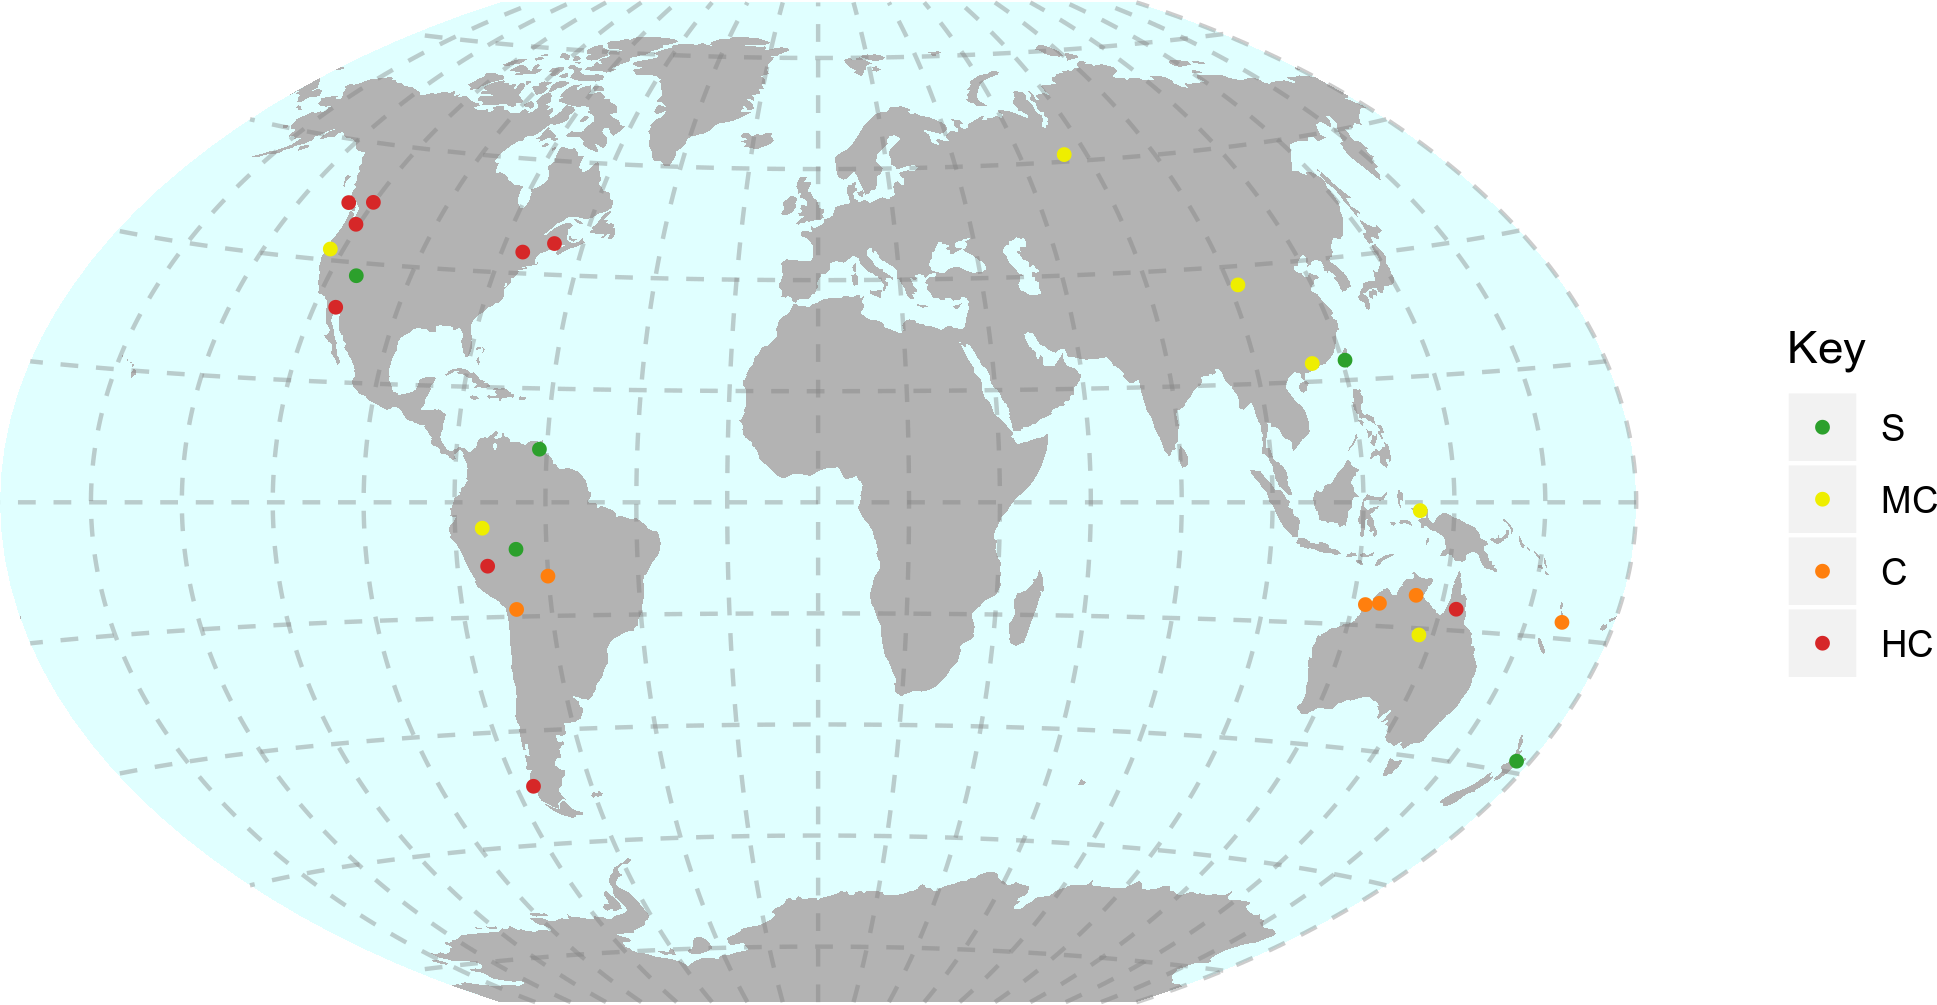
\includegraphics[width=\textwidth]{figures/fig46.png}
\caption{\label{fig:4.6}Areal distribution of languages in sample with no voicing contrast in obstruents.}
\end{figure}

  Indeed, the trend with respect to the \textit{voicing contrast in obstruents} feature is not significant in chi-square tests. Thus we do not find strong evidence for a relationship between phonation features and syllable structure complexity in this language sample.

\subsection{Place features}\label{sec:4.4.4}

  In this section I present an analysis of place features in the consonant phoneme inventories of the language sample. This analysis considers only the patterns of non-glide consonants. In \tabref{tab:4.13} I list the place features considered.

\begin{table}
\begin{tabularx}{\textwidth}{QQ}
\lsptoprule
Basic & Elaborated\\\midrule
labial-velar

bilabial

dental

alveolar

dental/alveolar

alveolo-palatal

palatal

velar

glottal & labiodental

palato-alveolar

retroflex

uvular

pharyngeal

palatalization

labialization

pharyngealization

velarization\\
\lspbottomrule
\end{tabularx}
\caption{\label{tab:4.13}Basic and elaborated place features examined here.}
\end{table}

  \figref{fig:4.7} shows how many languages in the sample each place feature is found in. Note that in the figure I have merged languages which have dental, alveolar or dental/alveolar articulations into one category of \textit{dental/alveolar}. This is to distinguish languages reported to have only one of these places of articulation from those reported to have both dental and alveolar articulations (the \textit{dental and alveolar} category).


\begin{figure}  
\caption{\label{fig:4.7} Place features in consonant inventories, by number of languages in which they are present.}
\end{figure}

  Several of the place features are (nearly) universal in the sample. All languages except for Mohawk have \textit{bilabial} consonants, and all but Wutung have \textit{velar} consonants. All languages in the sample have either \textit{dental/alveolar} or \textit{dental and alveolar} consonants; there is no trend with respect to syllable structure complexity for either of these features.

  There are five place features in the sample that are present in fewer than ten languages. The \textit{labial-velar} feature occurs in seven languages, six of which are spoken in Africa (Southern Bobo Madaré, Doyayo, Ewe, Southern Grebo, Lelepa, Ma’di, and Yoruba). Secondary \textit{palatalization} is present in six languages (Cocopa, Pinotepa Mixtec, Polish, Paiwan, Towa, and Urarina). The remaining rare place features are found only in languages with Highly Complex syllable structure. Secondary \textit{pharyngealization} and \textit{velarization} are present in one language each (Tashlhiyt and Albanian, respectively). \textit{Pharyngeal} consonants are found in languages from areas which are famous ‘hotspots’ of complex syllable structure: the Pacific Northwest (Nuu-chah-nulth, Thompson), the Caucasus (Kabardian), and the Atlas Mountains (Tashlhiyt).\footnote{{Here the term} \textrm{\textit{pharyngeal} }\textrm{also includes epiglottal consonants.}}

  The remaining eight place features — \textit{labiodental}, \textit{alveolo-palatal, palato-alveolar}, \textit{retroflex}, \textit{palatal}, \textit{uvular}, \textit{glottal}, and secondary \textit{labialization} — are found in more than ten languages each. Of these, there are three features which show a (near-)monotonic increase or decrease in frequency with respect to syllable structure complexity. These are shown in \figref{fig:4.8}.

\begin{figure}
\caption{\label{fig:4.8} Percentage of languages in each category of syllable structure complexity having the given place feature.}
\end{figure}

  There are two features in \figref{fig:4.8} which show strong positive trends with respect to syllable structure complexity. \textit{Palato-alveolars}, which are generally frequent in the language sample, are strongly associated with Highly Complex syllable structure, though the trend in this feature is not strictly linear between the Simple to Complex categories. This trend is statistically significant: χ\textsuperscript{2}(3, \textit{N} = 100) = 14.59, \textit{p} = .002. The \textit{uvular} pattern is especially striking. This place feature is distinctive in just one language (Sumi Naga) from the Simple category, yet its frequency of occurrence rises monotonically with syllable structure complexity to the extent that nearly half of the languages with Highly Complex syllable structure have consonants at this place of articulation. This trend is highly significant: χ\textsuperscript{2}(3, \textit{N} = 100) = 16.01, \textit{p} = .001. 

  The geographical distribution of uvulars is shown in \figref{fig:4.9}. While the prevalence of this feature in the Highly Complex syllable structure is boosted by its concentration in areas such as the Pacific Northwest and the Caucasus, it is notable that uvulars are also found to co-occur with Highly Complex syllable structure in regions as far-flung as New Guinea, Northeast Asia, and Patagonia.

\begin{figure}
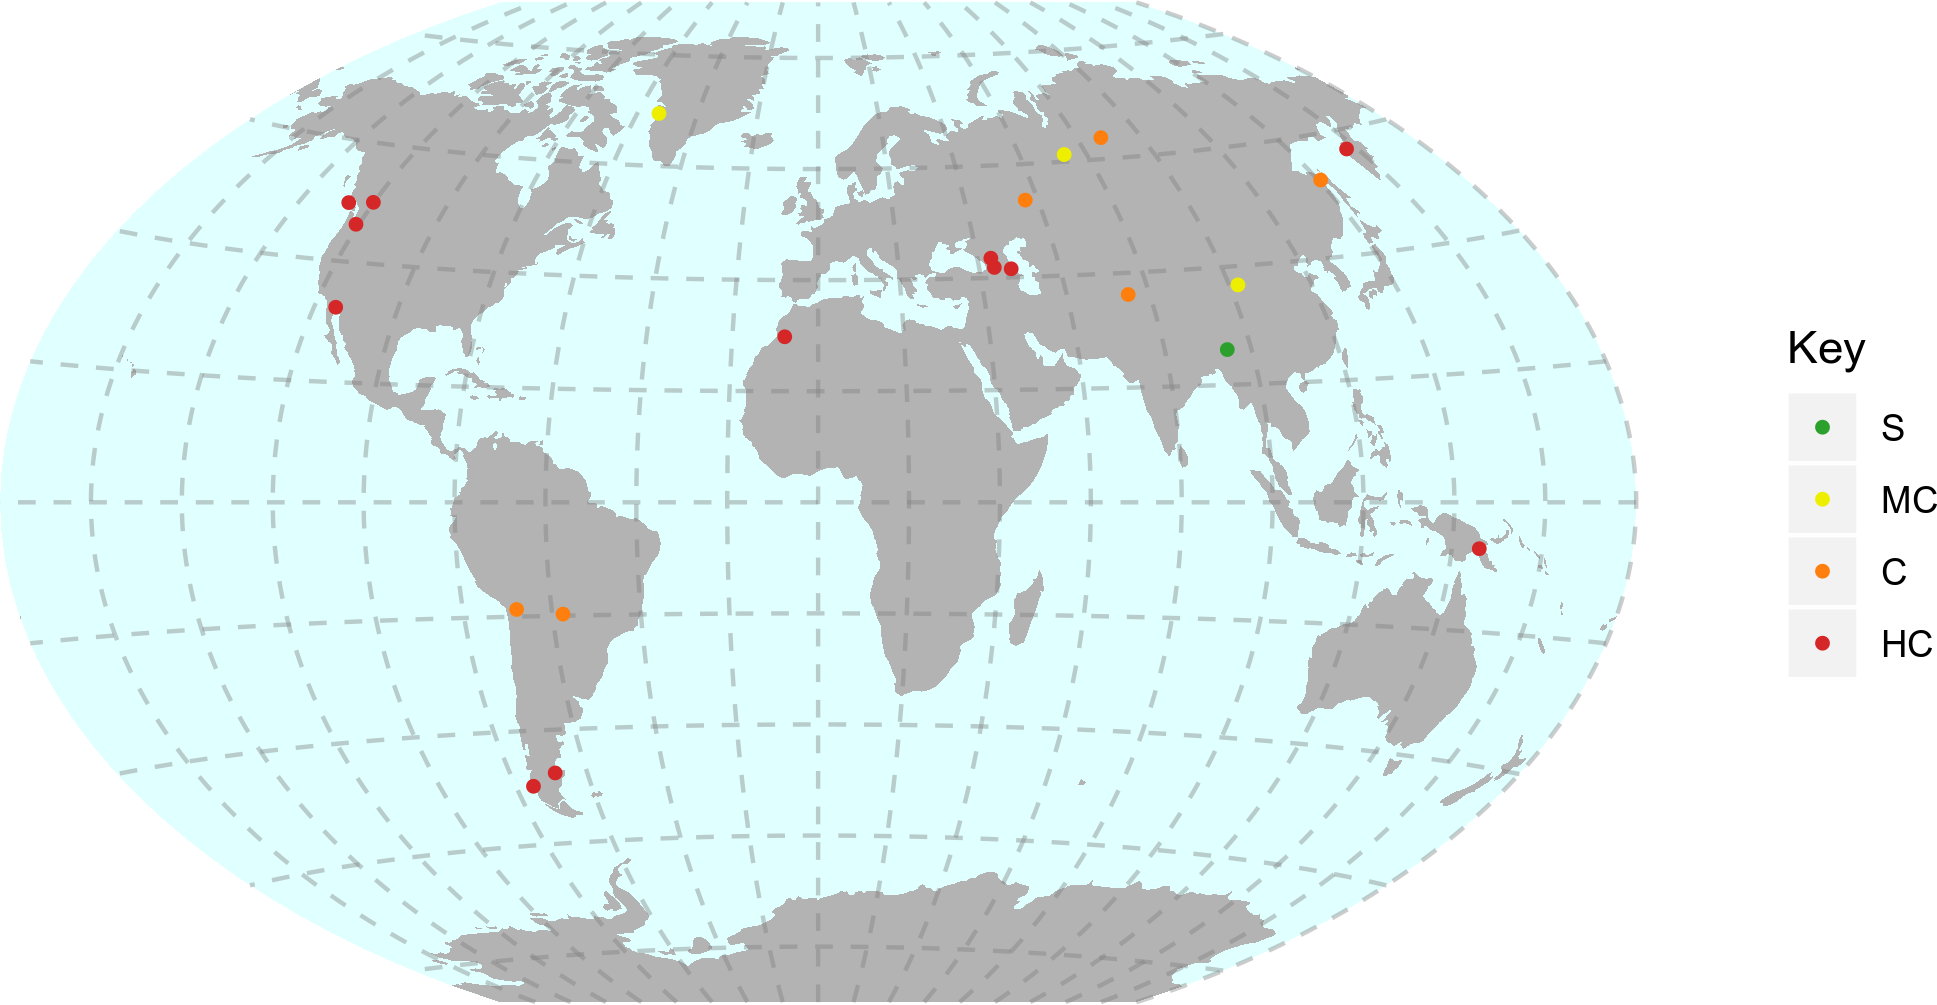
\includegraphics[width=\textwidth]{figures/fig49.png}
\caption{\label{fig:4.9}Areal distribution of languages in sample with uvular consonants.}
\end{figure}

  The \textit{palatal} articulation shows a negative trend with respect to syllable structure complexity. While this trend is not significant in a chi-square test, it is interesting that it runs counter to that established for \textit{palato-alveolars}. This observation brings up an important issue of terminology and description. It is not uncommon for authors of language descriptions to use the term ‘palatal’ in classifying the place of a series of consonants, but transcribe the consonants with the symbols used for palato-alveolars. Similarly, the terms ‘alveolo-palatal’ and ‘alveo-palatal’ may be used in prose descriptions, while palato-alveolar symbols are used in transcription. In her crosslinguistic study of palatalization, \citet{Bateman2007} notes that there is often disagreement on the transcription conventions used for secondarily palatalized velars, fronted velars, and palatal consonants. It is understandable that there is some inconsistency and interchangeability in the use of these terms: the area of contact between the tongue body and the hard palate may be large and variable in consonants articulated in this region, making it difficult to select a place classification (\citealt{LadefogedMaddieson1996}: 30-33). Since palato-alveolar and palatal places of articulation are not always reliably distinguished from one another or other similar articulations, we must consider the possibility that the trends with respect to these features in \figref{fig:4.8} effectively cancel each other out. In such a scenario, there would be no trend with respect to consonant articulations in this region of the vocal tract and syllable structure complexity.

  In order to clarify this issue, five places in the general region of the hard palate are examined: \textit{palato-alveolar}, \textit{palatal}, \textit{palatalized alveolar and/or velar}, and \textit{alveolo-palatal}. For each language, the number of places in which consonants are produced in this region is noted. For example, the phoneme inventory of Polish has consonants in three distinct places in this region: palato-alveolar, alveolo-palatal, and palatalized velar \REF{ex:4.32}.

\ea\label{ex:4.32}
\etriple{Polish}{Indo-European}{Poland}

\textbf{C phoneme inventory:} 

/p b pʲ bʲ t̪ d̪ k ɡ kʲ ɡʲ t̪͡s̪ d̪͡z̪ t͡ʃ d͡ʒ t͡ɕ d͡ʑ f v fʲ vʲ s̪ z̪ ʃ ʒ ɕ ʑ x m mʲ n̪ ɲ r l j w/
\z

  \figref{fig:4.10} shows the distribution of languages in the sample with respect to how many places are utilized in the region of the hard palate.

\begin{figure}
\caption{\label{fig:4.10} Number of place distinctions made in region of hard palate in languages with different syllable structure complexity. Place distinctions considered here are \textit{palato-alveolar}, \textit{palatal}, \textit{palatalized alveolar and/or velar}, and \textit{alveolo-palatal}. For each category of syllable structure complexity, I show the percentage of languages having one, two, three, or none of these places represented in their consonant inventories.}
\begin{tikzpicture}
\pgfplotstableread{data/fig410.csv}{\table}
    \pgfplotstablegetcolsof{\table}
    \pgfmathtruncatemacro\numberofcols{\pgfplotsretval-1}
            \begin{axis}[easterdaystacked,
                                xticklabels={Simple,{Moderately Complex},Complex,{Highly Complex}},
                        ]
            \foreach \i in {1,...,\numberofcols} {
                \addplot+[
                    /pgf/number format/read comma as period, fill
                    ] table [x index={1},y index={\i},x expr=\coordindex] {\table};
                \pgfplotstablegetcolumnnamebyindex{\i}\of{\table}\to{\colname} % Adding column headers to legend
                \addlegendentryexpanded{\colname}
            }
            \end{axis}                                                                           
\end{tikzpicture}
\end{figure}

  In all categories, most languages have at least one place articulation in the region of the hard palate. Crucially, the patterns in \figref{fig:4.10} show that the percentage of languages having one or more articulations in the region of the hard palate increases steadily with syllable structure complexity. That is, the trend favoring purported ‘palatal’ articulations in languages with simpler syllable structure does not cancel out the trend favoring purported ‘palato-alveolar’ articulations in languages with more complex syllable structure.

  Below I present another analysis of the proliferation of place distinctions in a large region of the vocal tract. In this case, the number of place distinctions made in the post-velar region is considered. The distinctions considered here are the \textit{uvular}, \textit{labialized uvular}, \textit{pharyngeal}, \textit{pharyngealized}, and \textit{glottal} places of articulation. \figref{fig:4.11} shows how the number of post-velar distinctions patterns with respect to syllable structure.

\begin{figure}
\caption{\label{fig:4.11} Number of place distinctions made in post-velar region in languages with different syllable structure complexity. Place distinctions considered here are \textit{uvular}, \textit{labialized uvular}, \textit{pharyngeal, pharyngealization}, and \textit{glottal}. For each category of syllable structure complexity, I show the percentage of languages having 1, 2, ${\geq}$3, or none of these places represented in their consonant inventories.}
\begin{tikzpicture}
\pgfplotstableread{data/fig411.csv}{\table}
    \pgfplotstablegetcolsof{\table}
    \pgfmathtruncatemacro\numberofcols{\pgfplotsretval-1}
            \begin{axis}[easterdaystacked,
                                xticklabels={Simple,{Moderately Complex},Complex,{Highly Complex}},
                        ]
            \foreach \i in {1,...,\numberofcols} {
                \addplot+[
                    /pgf/number format/read comma as period, fill
                    ] table [x index={1},y index={\i},x expr=\coordindex] {\table};
                \pgfplotstablegetcolumnnamebyindex{\i}\of{\table}\to{\colname} % Adding column headers to legend
                \addlegendentryexpanded{\colname}
            }
            \end{axis}                                                                           
\end{tikzpicture}
\end{figure}

  In all categories of syllable structure complexity, roughly similar proportions of languages have at least one post-velar place of articulation, usually glottal. However, in the Complex and Highly Complex categories, one-fifth and one-half of languages, respectively, have consonants at more than one place in the post-velar region. In fact, in the Highly Complex category, some languages have consonant systems which make use of four post-velar places (Kabardian, Nuu-chah-nulth, and Thompson), and one language (Tashlhiyt) has consonants at all five post-velar places. Below I show the consonant phoneme inventory of Nuu-chah-nulth, which has consonants at \textit{uvular}, \textit{labialized uvular}, \textit{pharyngeal}, and \textit{glottal} places of articulation \REF{ex:4.33}.

\ea\label{ex:4.33}
  \textbf{Nuu-chah-nulth} (\textit{Wakashan}; Canada)

\textbf{C phoneme inventory:} /p t k kʷ q qʷ ʕ ʔ p’ t’ k’ k’ʷ t͡s t͡ʃ t͡ɬ t͡s’ t͡ʃ’ t͡ɬ’ s ɬ ʃ x xʷ χ χʷ ħ h m n m’ n’ j w j’ w’/
\z

  In this section we have found that there are two place features of consonants which have statistically significant positive trends with respect to syllable structure complexity: \textit{uvular} and \textit{palato-alveolar} articulations (or at least one place in the region of the hard palate). Languages with more complex syllable structure also tend to have more consonant place articulations in the post-velar region, and infrequent post-velar articulations \textit{pharyngeal}, \textit{pharyngealization}, and \textit{velarization} are found only in languages with Highly Complex syllable structure in the current sample.

\subsection{Manner features}\label{sec:4.4.5}

  Here the manner features in the consonant phoneme inventories of the language sample are analyzed. In \tabref{tab:4.14} I list the manner features considered.

\begin{table}
\begin{tabularx}{\textwidth}{QQ}
\lsptoprule
{Basic} & {Elaborated}\\\midrule
stop

affricate

fricative

nasal

flap/tap

trill

central approximant

lateral affricate

lateral fricative

lateral flap

lateral approximant & prenasalization

nasal release

lateral release

ejective

implosive

click\\
\lspbottomrule
\end{tabularx}
\caption{\label{tab:4.14}Basic and elaborated manner features examined here. ‘Central approximants’ include non-lateral approximants such as glides but also ‘rhotic’ approximants like /ɹ/.}
\end{table}

  \figref{fig:4.12} shows how many languages in the sample have each manner feature. Because all instances of lateral release in the data were lateral affricates, these features have been merged so that only \textit{lateral release} is represented in the figure. \textit{Lateral flap} has also been merged with the more frequent (non-lateral) \textit{flap/tap} articulation.

  
\begin{figure}
\caption{\label{fig:4.12} Manner features in consonant inventories, by number of languages in which they are present.}
\end{figure}

  As with place features, there are several manner features which are (nearly) universal in the sample. \textit{Stops} occur in every language. \textit{Nasals} occur in all but two languages (Cubeo and Rotokas). There are four languages lacking \textit{fricatives}: Alyawarra, Bardi, Mangarrayi, and Ngarinyin. All of these languages are spoken in Australia, a region where this rare typological feature is common \citep[42]{Maddieson1984}. \textit{Central approximants} are reported to be absent in nine languages. However, in at least some of these languages, phonetic glides occur in complementary distribution with other sounds (e.g., Urarina, \citealt{Olawsky2006}: 37).

  There are five manner features occurring in ten or fewer languages in the sample. \textit{Clicks} and \textit{nasal release} occur in one language each (Hadza and Alyawarra, respectively). \textit{Implosives} are present in the consonant inventories of five languages, all from Africa and Southeast Asia \& Oceania: Doyayo, Tukang Besi, Sre, Ma’di, and Mpade. \textit{Lateral release}, which corresponds to lateral affricates, is found in only five languages, mostly from North America: Hadza, Nuu-chah-nulth, North Slavey, Thompson, and Yakima Sahaptin.

  The remaining seven manner features considered here — \textit{affricate}, \textit{flap/tap}, \textit{trill}, \textit{lateral fricative}, \textit{lateral approximant}, \textit{ejective}, \textit{prenasalization} — occur in more than ten languages each. Three of these —  \textit{flap/tap}, \textit{prenasalization}, and \textit{ejective} — show a (near-)monotonic increase or decrease with respect to syllable structure complexity. While the feature \textit{affricate} does not show a linear trend, it does show a large overall increase in frequency between the Simple and Highly Complex categories. The patterning of these four features with respect to syllable structure complexity can be found in \figref{fig:4.13}.

\begin{figure}
\caption{\label{fig:4.13} Percentage of languages in each category of syllable structure complexity having the given manner feature.}
\end{figure}

  There are two manner features whose frequency in inventories is associated with increasing syllable structure complexity. The trend in \textit{affricates}, though not linear, is nevertheless significant: χ\textsuperscript{2}(3, \textit{N} = 100) = 8.89, \textit{p} = .03. The \textit{ejectives} trend is statistically significant when the data from the Simple and Moderately Complex categories is combined and compared against that of the Complex and Highly Complex categories combined (\textit{p} =.006 in Fisher’s exact test). There is a heavy areal distribution of this feature: over half (10/19) of the languages with ejectives in the sample are found in the Americas. Outside the Americas, ejectives are also found to co-occur with Highly Complex syllable structure in the Caucasus region, Ethiopian Highlands, and Northeast Asia (see \figref{fig:4.14}).


\begin{figure}  
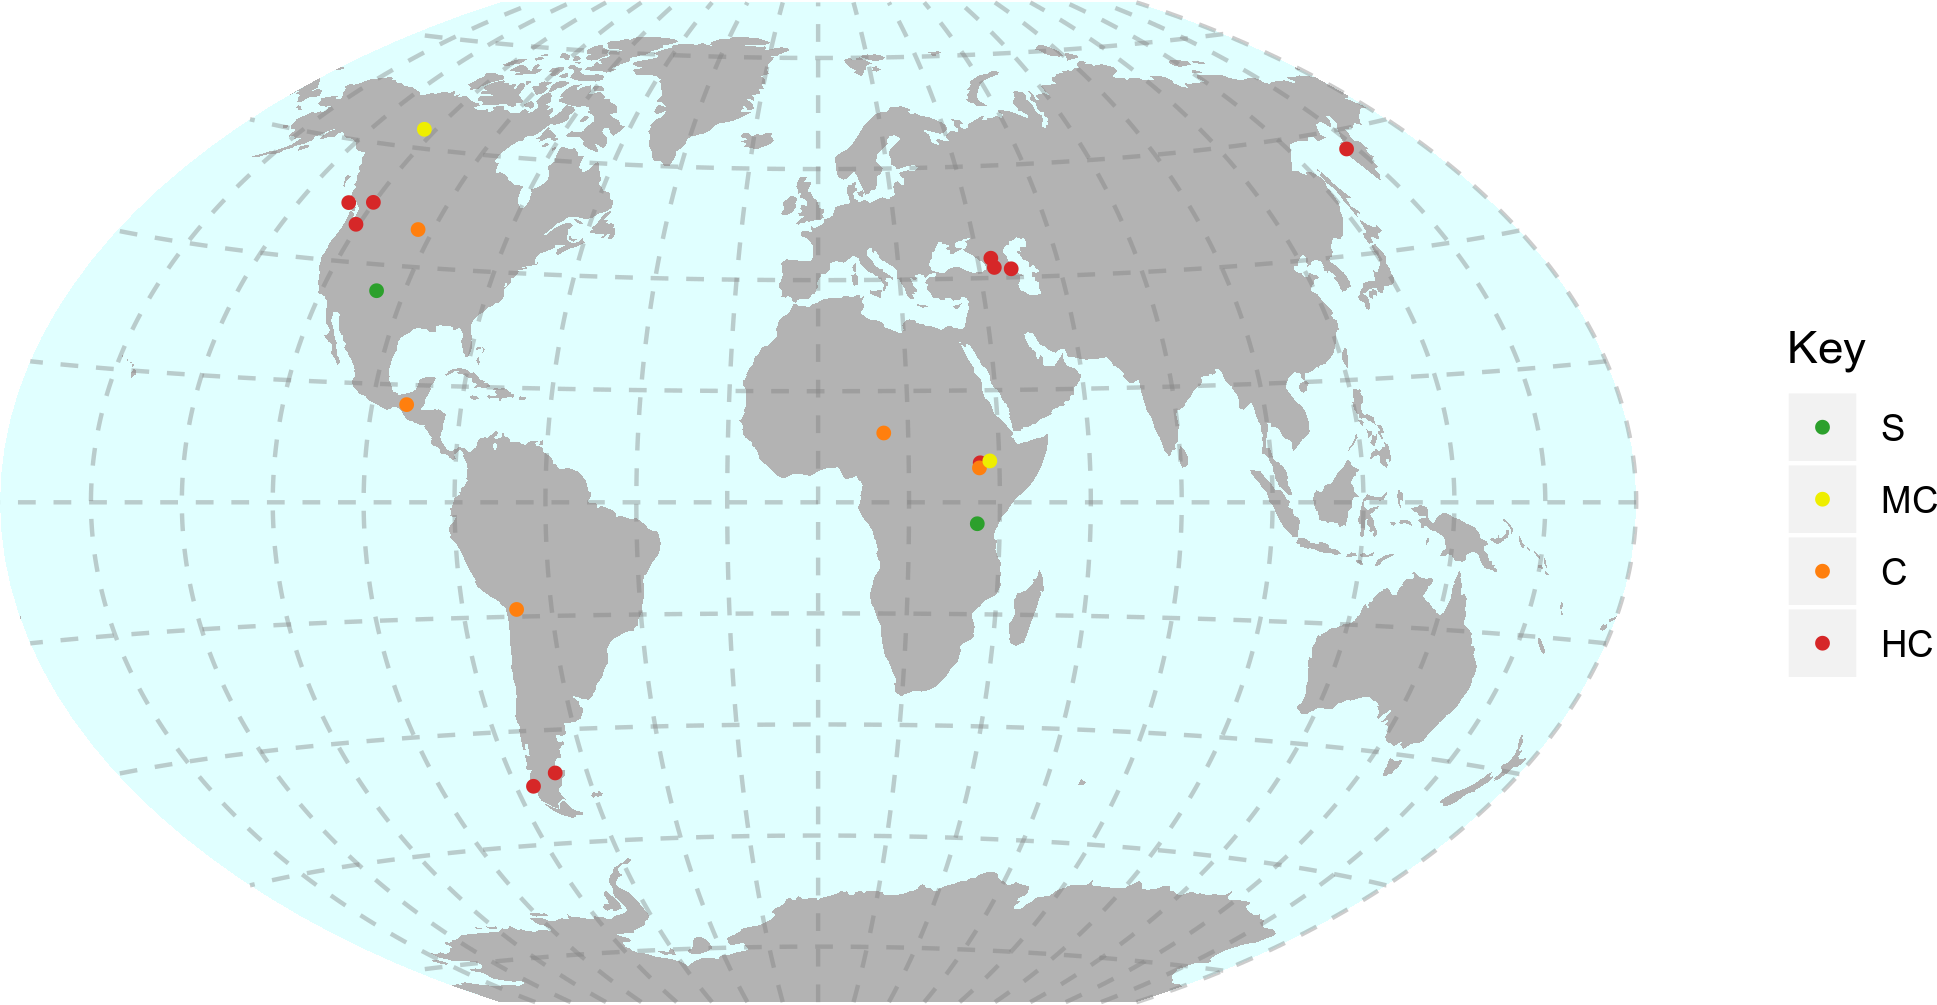
\includegraphics[width=\textwidth]{figures/fig414.png}
\caption{\label{fig:4.14}Areal distribution of languages in sample with ejective consonants.}
\end{figure}

The trend with affricates, though not linear, is 

  The proportion of languages with \textit{prenasalization} contrasts in their consonant phoneme inventories decreases with syllable structure complexity, though this trend is not statistically significant in a chi-square test. This trend is not clearly driven by any particular regional patterns: while roughly half (7/15) of languages with these articulations are from the region of Australia \& New Guinea, the distribution of those languages among the categories of syllable structure complexity is even. Further, the trend favoring prenasalization in languages with Simple syllable structure is not limited to a single region. The seven languages with Simple syllable structure and prenasalization are from four different macro-areas: Africa (Hadza, Ma’di), Australia \& New Guinea (East Kewa, Savosavo), North America (Pinotepa Mixtec), and Southeast Asia \& Oceania (Tukang Besi, Sichuan Yi). It is interesting to note that, like Simple syllable patterns, prenasalization contrasts tend to be found in languages spoken in close proximity to the equator (\figref{fig:4.15}).


\begin{figure}  
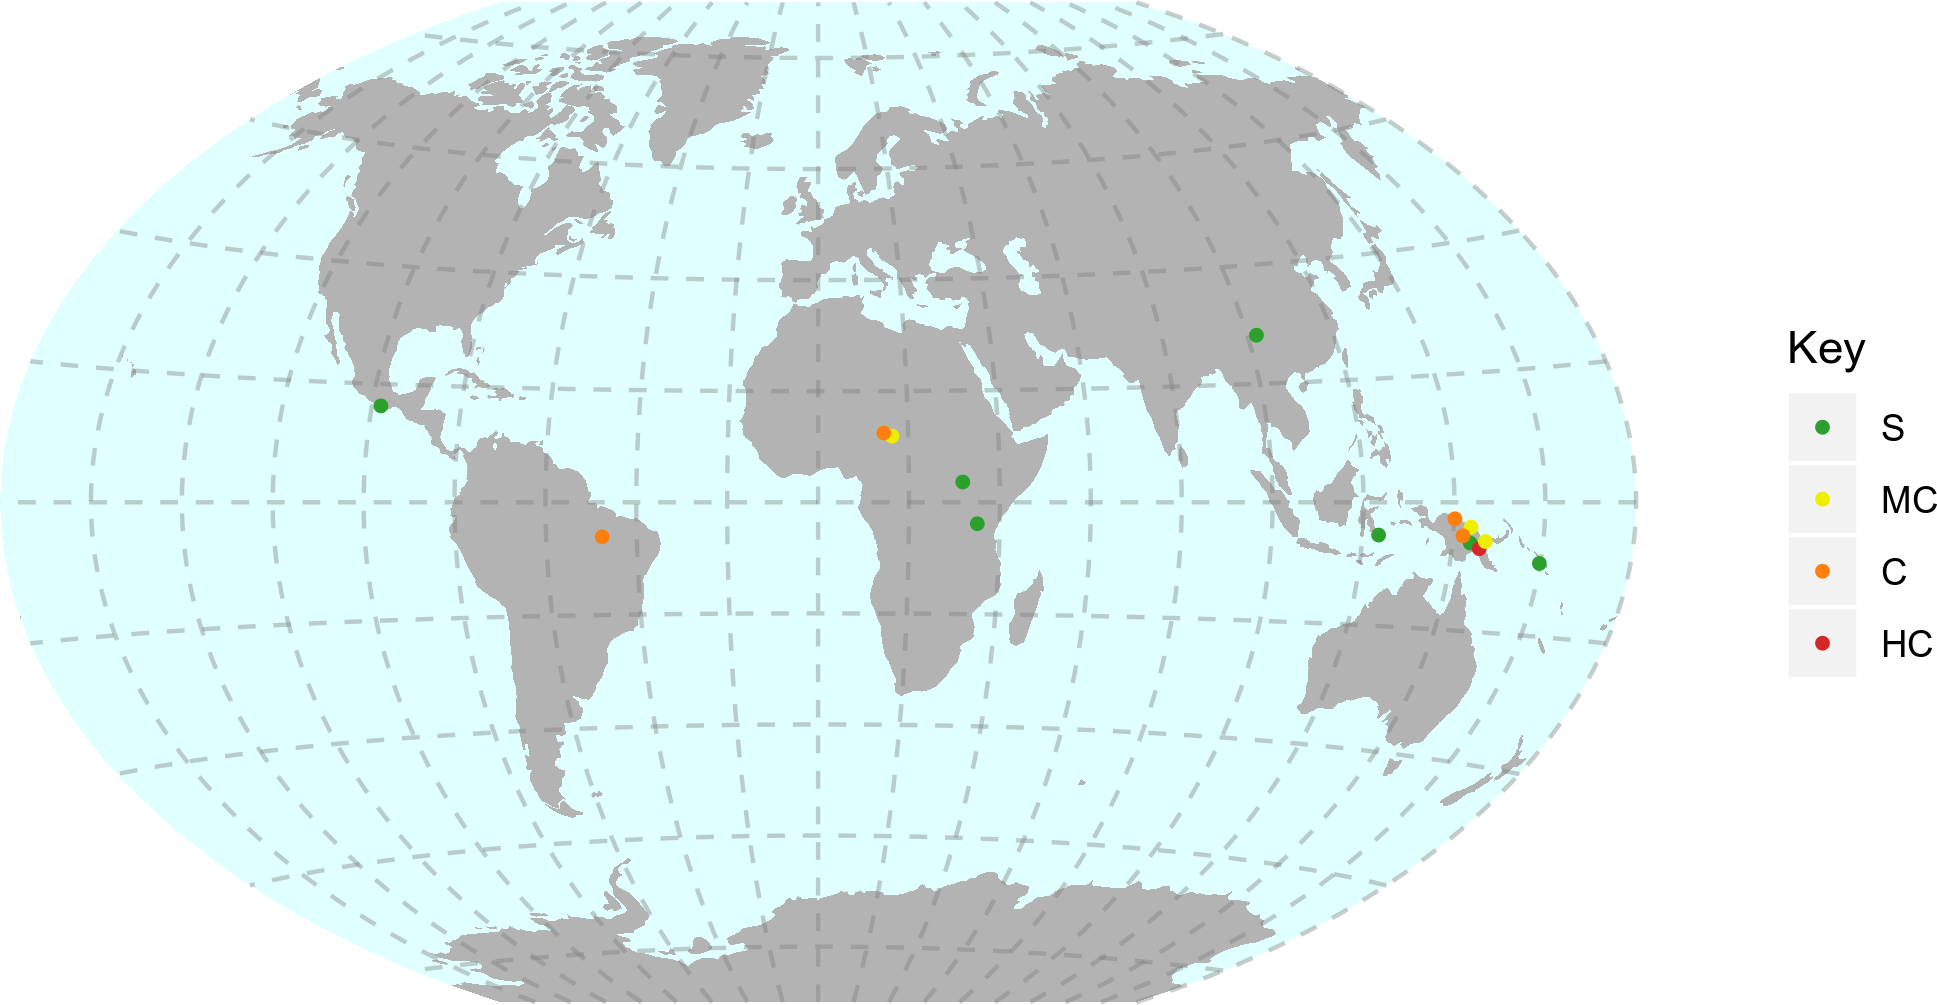
\includegraphics[width=\textwidth]{figures/fig415.png}
\caption{\label{fig:4.15}Areal distribution of languages in sample with prenasalized consonants.}
\end{figure}

  The \textit{flap/tap} feature also has a negative relationship with syllable structure complexity in the language sample, although this trend is not statistically significant in a chi-square test. Examining the geographical distribution of languages with flap or tap articulations, we find that this trend can be found within most of the macro-areas in the sample (\figref{fig:4.16}).


\begin{figure}  
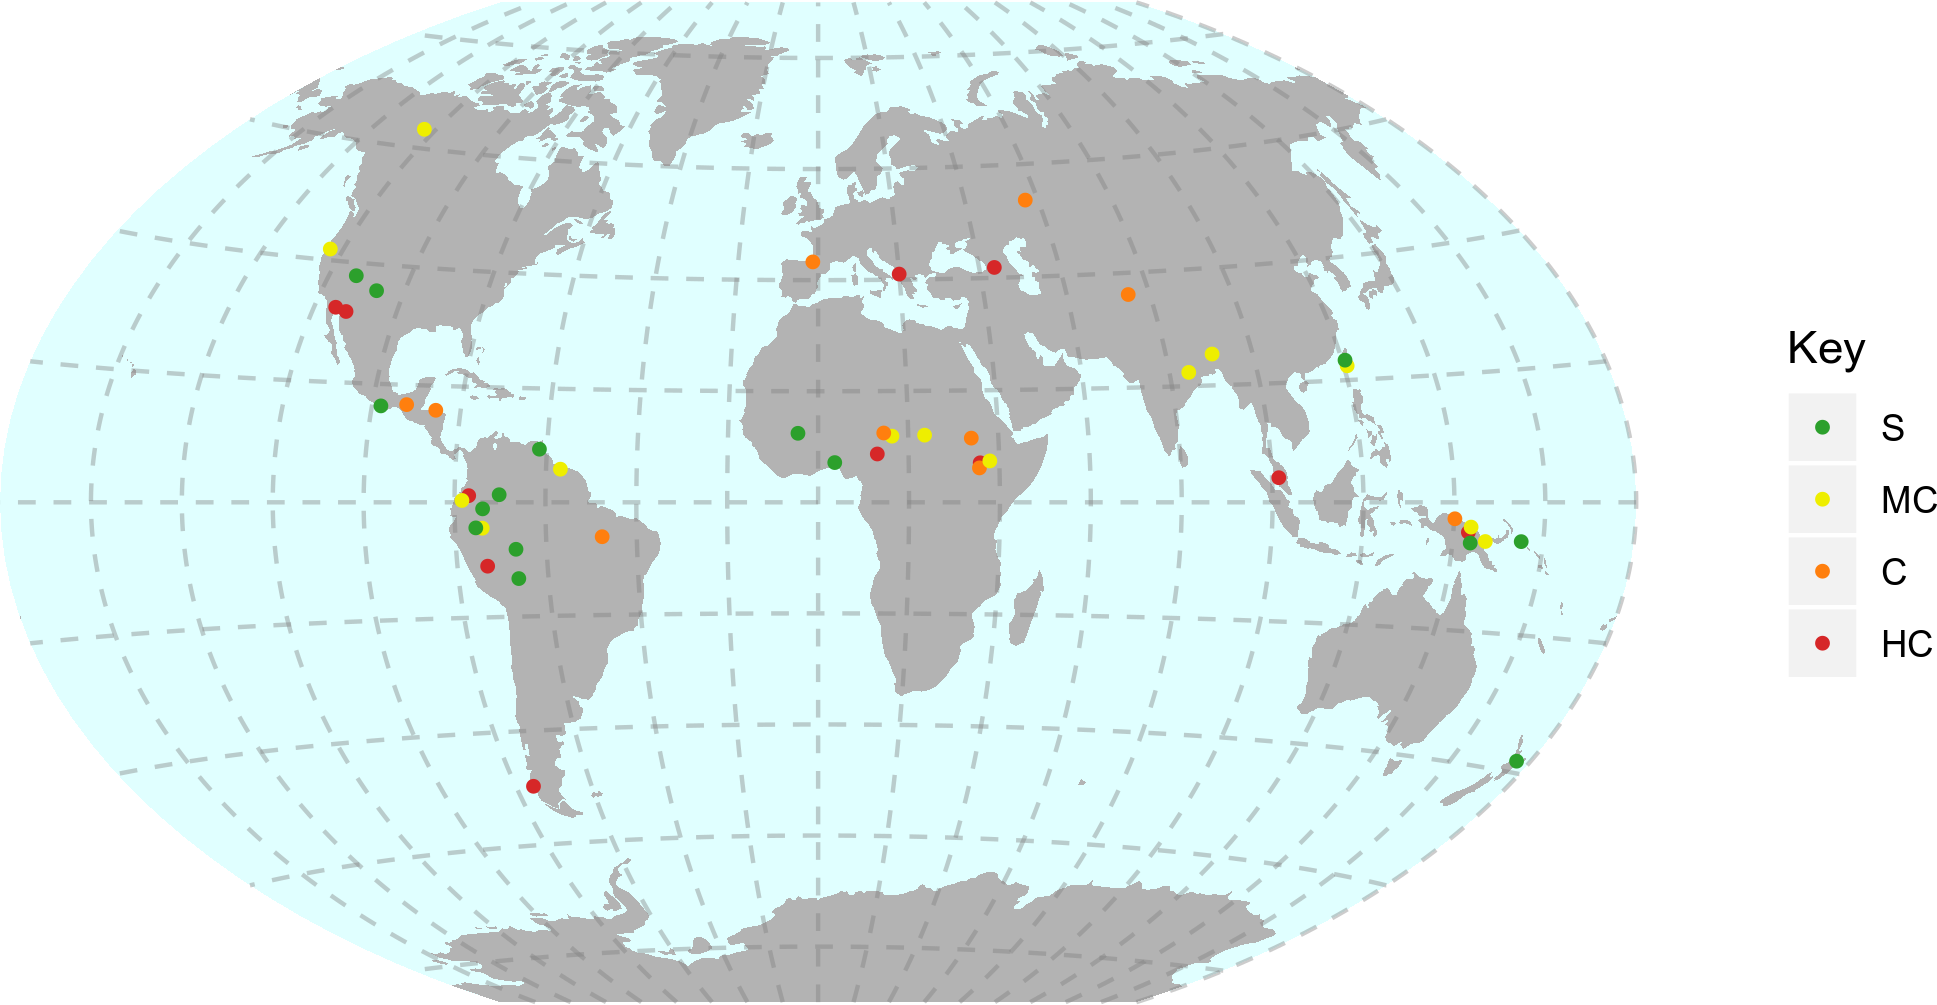
\includegraphics[width=\textwidth]{figures/fig416.png}
\caption{\label{fig:4.16}Areal distribution of languages in sample with flap/tap consonants.}
\end{figure}

  Flap and tap articulations differ from trill articulations in important ways. Flaps and taps are produced with a single rapid movement of the active articulator, usually the tongue tip, making brief contact with the passive articulator, usually the alveolar ridge. Trills in the coronal region often have the same configuration of articulators, but the movement of the active articulator is a vibration driven by aerodynamic currents rather than muscular movements (\citealt{LadefogedMaddieson1996}: 217-32). However, taps and flaps can vary allophonically with trills in some languages. We must allow for the possibility that the trend noted above reflects an analytical preference, in languages with simpler syllable structure, by which the flap/tap articulation is considered primary in such cases of allophonic variation. \figref{fig:4.17} shows how flap/tap and coronal trill articulations are distributed among languages with different syllable structure complexity. Even in the most liberal interpretation of the analytical preference scenario, the pattern with trill articulations does not clearly neutralize the pattern of flap/tap articulations.

\begin{figure}
\begin{tikzpicture}
\pgfplotstableread{data/fig417.csv}{\table}
    \pgfplotstablegetcolsof{\table}
    \pgfmathtruncatemacro\numberofcols{\pgfplotsretval-1}
            \begin{axis}[easterdaystacked,
                                xticklabels={Simple,{Moderately Complex},Complex,{Highly Complex}},
                        ]
            \foreach \i in {1,...,\numberofcols} {
                \addplot+[
                    /pgf/number format/read comma as period, fill
                    ] table [x index={1},y index={\i},x expr=\coordindex] {\table};
                \pgfplotstablegetcolumnnamebyindex{\i}\of{\table}\to{\colname} % Adding column headers to legend
                \addlegendentryexpanded{\colname}
            }
            \end{axis}                                                                           
\end{tikzpicture}
\caption{\label{fig:4.17} Distribution of languages with flap/tap and trill articulations, by syllable structure complexity.}
\end{figure}

  In this section we have found statistically significant trends positively associating \textit{affricate} and \textit{ejective} manners of articulation with syllable structure complexity. We also find weaker trends which are not statistically significant showing a negative association between the presence of \textit{flap/tap} and \textit{prenasalized} articulations and syllable structure complexity.

\subsection{Summary of consonant patterns in sample}\label{sec:4.4.6}

  Three hypotheses were formulated in \sectref{sec:4.1.4} with respect to consonant inventory patterns and syllable structure complexity. First, it was hypothesized that consonant phoneme inventory size would increase with syllable structure complexity. This relationship was upheld in the current sample and was found to be statistically significant. Second, it was hypothesized that the number of elaborated articulations present in consonant phoneme inventories would increase with syllable structure complexity. As expected, this correlation was found to be positive and significant, though the difference in average number of elaborations was not dramatic between the categories at the two extremes of syllable structure complexity. Finally, it was hypothesized that languages with more complex syllable structure would have different kinds of consonants in their inventories than languages with simpler syllable structure. The results of the analyses in \sectref{sec:4.4.3}-5 suggest that this is the case, as there are specific consonant articulations which are more frequently present in languages of the Complex and Highly Complex categories. However, it was also found that there are consonant types which occur more frequently in languages with simpler syllable structures. Thus it can be said, more generally, that languages with different syllable patterns also tend to have different kinds of consonants in their phoneme inventories.

  Trends positively associating \textit{uvular}, \textit{palato-alveolar}, \textit{affricate}, and \textit{ejective} articulations with syllable structure complexity were found to be statistically significant in the current language sample, while trends negatively associating a \textit{voicing contrast in obstruents}, \textit{palatals}, \textit{flaps/taps} and \textit{prenasalization} with syllable complexity were not found to be statistically significant. However, given the relatively small sample size considered, it is possible that different results might be found for all of these trends in a larger sample. The robustness of each of these trends was investigated in the 501 publicly-available languages in LAPSyD \citep{MaddiesonEtAl2013}. Within LAPSyD, it was found that most of these articulations — all except for \textit{voicing contrast in obstruents} and \textit{palatals} — have weak but highly significant positive or negative correlations with syllable structure complexity (measured as the sum of maximal syllable margins). These verified correlations, which correspond in directionality to those patterns established above, are listed and marked by asterisks in \tabref{tab:4.15}. Additionally, the table lists in italics two general trends established in the present study with respect to articulations in the palatal and postvelar regions.

\begin{table}
\begin{tabular}{llS[table-format=1.3]S[table-format=<1e1]}
\lsptoprule

{Type of feature} & {Articulation} & \multicolumn{2}{c}{Correlation in LAPSyD}\\\cmidrule(lr){3-4}
                  &                &  {$r(501)$}      &   {$p$}\\\midrule
{Place} & *Palato-alveolar & .162 & <5e-04\\
        & *Uvular  & .282 & <1e-05\\
& \multicolumn{3}{l}{\textit{At least one distinction in palatal region}}\\
& \multicolumn{3}{l}{\textit{More post-velar distinctions}}\\
{Manner} & *Affricate & .156 & <5e-04\\
         & *Ejective  & .180 & <1e-04\\
         & *Flap/tap  & -.136 & .002\\
         & *Prenasalization & -.175 & <1e-04\\
\lspbottomrule
\end{tabular}
\caption{\label{tab:4.15}Features of consonantal systems associated positively or negatively with syllable structure complexity. Where relevant, the statistically significant correlation in LAPSyD \citep{MaddiesonEtAl2013} is given.\todo[inline]{Is the remark in italics placed correctly?}}
\end{table}

  There is an important general observation to be made regarding the patterns uncovered here. This is that the three standard aspects of consonant articulation examined here — phonation, place, and manner — pattern differently with respect to syllable structure complexity. Phonation features do not seem to be correlated with syllable structure complexity. The presence of certain place features is associated with more complex syllable structure. Both ends of the syllable structure complexity scale are associated with specific manner features, but very different kinds. The manners of articulation associated with more complex syllable structure (affricates and ejectives) are obstruents, while the manner features associated with simpler syllable structure are either sonorants (flap/tap), or arguably have a sonorant component (prenasalized consonants). These patterns may have important implications for uncovering the development of highly complex syllable structure, as well as for establishing a syllable structure-based phonological typology of languages. These issues will be discussed further in \sectref{sec:4.5}.

\section{Discussion}\label{sec:4.5}
\subsection{Segmental inventory patterns and syllable structure complexity}\label{sec:4.5.1}

  In light of the findings presented in the current chapter, we revisit the first broad research goal of this work, which is to determine whether languages with highly complex syllable structure share other characteristics such that this group can be classified as a holistic language type.

  The results indicate that there are a number of specific segmental patterns associated with highly complex syllable structure, all of which are related to consonants. These are summarized in \REF{ex:4.34}. The terms ‘absence’ and ‘presence’ are used here not in a categorical sense, but to mean relative absence or presence of a property in the Highly Complex group as compared to the other syllable structure complexity groups.

\ea\label{ex:4.34}
  \textbf{Segmental patterns associated with Highly Complex category}

\textit{Mean of 26 consonant phonemes}

\textit{Mean of 4 elaborations in consonant phoneme inventory}

\textit{Absence of prenasalized consonants}

\textit{Absence of flap/tap consonants}

\textit{Presence of palato-alveolar consonants}

\textit{Presence of uvular consonants}

\textit{Presence of affricate consonants} 

\textit{Presence of ejective consonants}
\z

  This list does not include two more general segmental patterns of languages with Highly Complex syllable structure: at least one place distinction in the region of the hard palate, and a more richly elaborated set of place distinctions in the post-velar region.

  Recall the analyses in \sectref{sec:3.4.1}-2 which established two different distributions in the languages of the Highly Complex category. In eight languages — Cocopa, Georgian, Itelmen, Polish, Tashlhiyt, Thompson, Tohono O’odham, and Yakima Sahaptin — Highly Complex structures were found to be a prevalent pattern. In six languages — Alamblak, Bench, Doyayo, Kunjen, Menya, and Wutung — Highly Complex structures were found to be a minor pattern. As discussed in \chapref{sec:3}, the languages within each of these groups share similar patterns with respect to the occurrence of Highly Complex structures at each syllable margin, restrictions on consonant combinations in these structures, and the relative frequency of these structures. The 11 languages which belong to neither group — Albanian, Camsá, Kabardian, Lezgian, Mohawk, Nuu-chah-nulth, Passamaquoddy-Maliseet, Yine, Qawasqar, Semai, and Tehuelche — have syllable patterns which vary with respect to the different features examined or which fall somewhere in between the patterns of the two extreme groups.

  It is reasonable to expect that if highly complex syllable structure has other phonetic and phonological correlates, then languages which differ in the extent to which these syllable structures are prominent might also exhibit the other correlates to different degrees. In \tabref{tab:4.16} the languages of the Highly Complex portion of the sample are divided into the three groups described above. The properties of vowel and consonant inventories associated with Highly Complex syllable structure and listed in \REF{ex:4.34} above are given in the columns. A check mark indicates that a language has the expected property; a shaded cell indicates that it does not. For consonant phoneme inventory size and number of elaborations, I have designated a value greater than or equal to the mean for the category to be the expected property.

\begin{table}
\begin{tabularx}{\textwidth}{lCCCCCCCC}
\lsptoprule
 & \textbf{${\geq}$ 26} Cs & \textbf{${\geq}$ 4} elabs. & Prenasalization absent & Flap\slash tap absent & Palato-alveolar present & Uvular present & Affricate present & Ejective present\\\midrule
& \multicolumn{8}{c}{Languages with prevalent Highly Complex patterns}\\\midrule
 Cocopa & \cellcolor{lsLightGray} & \ding{51} & \ding{51} & \ding{51} & \ding{51} & \ding{51} & \ding{51} & \cellcolor{lsLightGray}\\
 Georgian & \ding{51} & \ding{51} & \ding{51} & \cellcolor{lsLightGray} & \ding{51} & \ding{51} & \ding{51} & \ding{51}\\
 Itelmen & \cellcolor{lsLightGray} & \ding{51} & \ding{51} & \ding{51} & \ding{51} & \ding{51} & \ding{51} & \ding{51}\\
 Polish & \ding{51} & \ding{51} & \ding{51} & \ding{51} & \ding{51} & \cellcolor{lsLightGray} & \ding{51} & \cellcolor{lsLightGray}\\
 Tashlhiyt & \ding{51} & \ding{51} & \ding{51} & \ding{51} & \ding{51} & \ding{51} & \cellcolor{lsLightGray} & \cellcolor{lsLightGray}\\
 Thompson & \ding{51} & \ding{51} & \ding{51} & \ding{51} & \ding{51} & \ding{51} & \ding{51} & \ding{51}\\
 T. O’odham & \cellcolor{lsLightGray} & \cellcolor{lsLightGray} & \ding{51} & \cellcolor{lsLightGray} & \ding{51} & \cellcolor{lsLightGray} & \ding{51} & \cellcolor{lsLightGray}\\
 Y. Sahaptin & \ding{51} & \ding{51} & \ding{51} & \ding{51} & \ding{51} & \ding{51} & \ding{51} & \ding{51}\\\midrule
& \multicolumn{8}{c}{Languages with intermediate Highly Complex patterns}\\\midrule
 Albanian & \ding{51} & \ding{51} & \ding{51} & \cellcolor{lsLightGray} & \ding{51} & \cellcolor{lsLightGray} & \ding{51} & \cellcolor{lsLightGray}\\
 Camsá & \cellcolor{lsLightGray} & \cellcolor{lsLightGray} & \ding{51} & \cellcolor{lsLightGray} & \ding{51} & \cellcolor{lsLightGray} & \ding{51} & \cellcolor{lsLightGray}\\
 Kabardian & \ding{51} & \ding{51} & \ding{51} & \ding{51} & \ding{51} & \ding{51} & \ding{51} & \ding{51}\\
 Lezgian & \ding{51} & \ding{51} & \ding{51} & \ding{51} & \ding{51} & \ding{51} & \ding{51} & \ding{51}\\
 Mohawk & \cellcolor{lsLightGray} & \cellcolor{lsLightGray} & \ding{51} & \ding{51} & \ding{51} & \cellcolor{lsLightGray} & \ding{51} & \cellcolor{lsLightGray}\\
 Nuu-chah-nulth & \ding{51} & \ding{51} & \ding{51} & \ding{51} & \ding{51} & \ding{51} & \ding{51} & \ding{51}\\
 P. - Maliseet & \cellcolor{lsLightGray} & \cellcolor{lsLightGray} & \ding{51} & \ding{51} & \ding{51} & \cellcolor{lsLightGray} & \ding{51} & \cellcolor{lsLightGray}\\
 Yine & \cellcolor{lsLightGray} & \cellcolor{lsLightGray} & \ding{51} & \cellcolor{lsLightGray} & \ding{51} & \cellcolor{lsLightGray} & \ding{51} & \cellcolor{lsLightGray}\\
 Qawasqar & \cellcolor{lsLightGray} & \cellcolor{lsLightGray} & \ding{51} & \ding{51} & \cellcolor{lsLightGray} & \ding{51} & \ding{51} & \ding{51}\\
 Semai & \cellcolor{lsLightGray} & \cellcolor{lsLightGray} & \ding{51} & \cellcolor{lsLightGray} & \cellcolor{lsLightGray} & \cellcolor{lsLightGray} & \cellcolor{lsLightGray} & \cellcolor{lsLightGray}\\
 Tehuelche & \cellcolor{lsLightGray} & \cellcolor{lsLightGray} & \ding{51} & \ding{51} & \ding{51} & \ding{51} & \ding{51} & \ding{51}\\\midrule
& \multicolumn{8}{c}{Languages with minor Highly Complex patterns}\\\midrule
 Alamblak & \cellcolor{lsLightGray} & \cellcolor{lsLightGray} & \ding{51} & \cellcolor{lsLightGray} & \ding{51} & \cellcolor{lsLightGray} & \ding{51} &\cellcolor{lsLightGray} \\
 Bench & \ding{51} & \cellcolor{lsLightGray} & \ding{51} & \cellcolor{lsLightGray} & \ding{51} & \cellcolor{lsLightGray} & \ding{51} & \ding{51}\\
 Doyayo & \cellcolor{lsLightGray} & \cellcolor{lsLightGray} & \ding{51} & \cellcolor{lsLightGray} & \cellcolor{lsLightGray} & \cellcolor{lsLightGray} & \cellcolor{lsLightGray} & \cellcolor{lsLightGray}\\
 Kunjen & \cellcolor{lsLightGray} & \ding{51} & \ding{51} & \ding{51} & \cellcolor{lsLightGray} & \cellcolor{lsLightGray} & \cellcolor{lsLightGray} & \cellcolor{lsLightGray}\\
 Menya & \cellcolor{lsLightGray} & \ding{51} & \cellcolor{lsLightGray} & \ding{51} & \ding{51} & \ding{51} & \ding{51} & \cellcolor{lsLightGray}\\
 Wutung & \cellcolor{lsLightGray} & \cellcolor{lsLightGray} & \ding{51} & \ding{51} & \ding{51} & \cellcolor{lsLightGray} & \ding{51} & \cellcolor{lsLightGray}\\
\lspbottomrule
\end{tabularx}
\caption{\label{tab:4.16}Highly Complex languages, divided into three groups according to the prominence of their Highly Complex patterns. Check mark indicates that the given language has the expected segmental property; shaded cell indicates it does not.}
\end{table}

  The visual pattern in \tabref{tab:4.16} indicates that the expectations are borne out. Languages which have Highly Complex syllable structure as a prevalent pattern also tend to have more of the established segmental correlates of Highly Complex syllable structure. Languages which have Highly Complex syllable structure as a minor pattern tend to have fewer of the segmental correlates. The ‘intermediate’ languages have a pattern that is intermediate between the two. It is striking that the three subtypes of Highly Complex syllable structure, which were defined entirely by reference to their syllable patterns, show the predicted patterns with respect to the presence of segmental correlates of Highly Complex syllable structure.

  Five languages have all of the established segmental correlates of Highly Complex syllable structure. Their consonant inventories might be considered to be prototypical of the Highly Complex category. To illustrate, I give the consonant inventory of Yakima Sahaptin in \REF{ex:4.35}.

\ea\label{ex:4.35}
\etriple{Yakima} \textbf{Sahaptin}{Sahaptian}{USA}

\textbf{C phoneme inventory:} 

/p t k kʷ q qʷ ʔ p’ t’ k’ k’ʷ q’ q’ʷ t͡ɬ t͡s t͡ʃ t͡ɬ’ t͡s’ t͡ʃ’ ɬ s ʃ x xʷ χ χʷ h m n l w j/
\z

  The results of the analyses in this chapter also reveal tendencies in the segmental patterns of languages on the Simple end of the syllable structure complexity cline. In most cases these patterns are the opposite of those consonantal properties given in \REF{ex:4.34} for the Highly Complex category. However, some of the segmental patterns observed in this category are more extreme than others. In the case of uvulars and ejectives, there is a near absence of this consonant type in languages with Simple syllable structure. Additionally, there are three segmental properties of vowels, including the absence of a length contrast of vowels, the presence of a nasalization contrast in vowels, and the presence of a vowel phonation contrast, which show patterns favoring Simple syllable structure. Finally, languages with Simple syllable structure have the lowest mean number of consonant phonemes (21 consonants) of all the categories examined here.

  It is important to keep in mind that the findings reported here are tendencies, some of them quite subtle. Languages in the sample also show wide variation in the structuring of their segmental inventories, resulting in many exceptions to the general patterns. Hadza is in the Simple category, yet has the largest consonant inventory and number of elaborations of all the languages.\footnote{{Borrowing may account for some of the sounds in the Hadza phoneme inventory. Bonny Sands (p.c.) notes that it is possible that some click articulations have been borrowed from other click languages, in the same way that some Bantu languages have borrowed clicks from neighboring Khoisan languages. Kirk Miller (p.c.) suggests that Hadza seems to have borrowed its initial prenasalized consonants and all voiced obstruents besides /b/. Even excluding clicks and non-bilabial voiced obstruents, the language would have a consonant inventory of 41 segments, which is still quite large. Sands and Miller agree that, apart from the presence of clicks, the phoneme inventory of Hadza is not atypical for an East African, and particularly Cushitic, language.}} Mohawk and Passamaquoddy-Maliseeet are in the Highly Complex category, yet have very small consonant inventories and few articulatory elaborations. However, it is encouraging for the wider implications of this study that several of the general findings, such as those regarding consonant phoneme inventory size and consonant elaborations, replicate the results of previous studies with much larger sample sizes or can be verified in LAPSyD (\citealt{MaddiesonEtAl2013}, 501 languages). It is also notable that the distribution of features correlated with languages at either end of the syllable structure complexity cline does not appear to be random. The Highly Complex category is coherently associated with a group of consonant place features and manner features related to obstruents. The Simple category is coherently associated with two manner features related to sonorants. This point will be discussed further in the following sections.

  Having established segmental correlates of syllable structure complexity, we revisit the second research question of the book: how does highly complex syllable structure develop over time? The segment inventory of a language reflects, at least in part, sound changes which occurred at some point in the history of the language. Some typologically frequent speech sounds — for instance, voiceless stops at labial, dental/alveolar, and velar places of articulation — tend to persist within sound systems over the history of a language, and are not often observed to come about from other sounds as the result of allophonic processes (\citealt{Bybee2015a}; see also discussion in \sectref{sec:4.1.1}). This tendency may reflect general biological constraints on the vocal tract and/or the perceptual robustness of these sounds. However, for many other sounds, there is evidence for how they tend to develop through phonetic mechanisms in language use. 

  In \sectref{sec:4.5.2} I discuss reported processes of sound change which result in the consonantal patterns associated with Highly Complex syllable structure. In \sectref{sec:4.5.3} I discuss reported processes resulting in the consonantal patterns associated with Simple syllable structure. In the following I include historical, comparative, and synchronic accounts of sound change processes. Although historical evidence is best because it involves more or less direct observation, the history of written language is such that there are very few languages, language families, and regions for which such evidence exists on a deep time scale. Including reports of synchronic and comparative processes greatly expands the range of data available, but it does come with the caveat that the reported patterns may have other possible analyses. Many of the synchronic processes reported here are from AlloPhon, a database of over 800 phonetically-conditioned processes in 81 diverse languages (\citealt{BybeeEasterday2019}).

  In \sectref{sec:4.5.4}, I compare the patterns reported in \sectref{sec:4.5.2}-3 and discuss their broad implications with respect to the diachronic development of highly complex syllable structure and syllable typology more generally.

\subsection{Articulations and contrasts characteristic of the Highly Complex category} \label{sec:4.5.2}

  In this section I present historical, comparative, and synchronic accounts of processes resulting in articulations and contrasts associated with the Highly Complex category, specifically palato-alveolars, uvulars, ejectives, and affricates. Additionally, as a more richly elaborated set of post-velar consonant distinctions is associated with this category, I also discuss the historical development of pharyngeals. As will be discussed in \sectref{sec:4.5.4}, all of these articulations commonly come about through the place assimilation of consonants to vowels and strengthening processes.

\subsubsection{{Palato-alveolars}}\label{sec:4.5.2.1}

  Palato-alveolars are articulations made with the tongue blade in the area of the hard palate behind the alveolar ridge. These are known to develop from many different kinds of consonants. The most common conditioning environments for the development of these sounds are front, especially high front, vowels and palatal glides. Thus palato-alveolars are often a product of the crosslinguistically common process of palatalization (\citealt{Bhat1978}; \citealt{Bateman2007,BybeeEasterday2019}). Typically, the consonant undergoing palatalization precedes the conditioning vowel or glide. In a common type of process, palato-alveolars may develop out of alveolar consonants preceding a high front vowel, as in synchronic processes in Cantonese \REF{ex:4.36} and Logba \REF{ex:4.37}.

\ea\label{ex:4.36}
  \textbf{Cantonese} (\textit{Sino-Tibetan}; China)

/t͡sy/

[t͡ʃy]\\
\glt ‘live’

(\citealt{MatthewsYip1994}: 14)
\z

\ea\label{ex:4.37}
  \textbf{Logba} (\textit{Atlantic-Congo}; Ghana)

/onziɛ/

[onʒiɛ]\\
\glt ‘owl’
\citep[18]{Dorvlo2008}
\z

  Palato-alveolars are also known to develop out of velar consonants. The usual situation involves a velar stop becoming a palato-alveolar affricate preceding a high front vowel or glide. A well-known example of this occurred in the late stages of Latin and early stages of Romance, when velar stops were fronted preceding front vowels, then eventually became palato-alveolar affricates in some of the daughter languages, e.g. Latin [k]\textit{ivitate} > Italian [t͡ʃ]\textit{ittà} ‘city’ \citep[113]{Posner1996}. \citet{Bhat1978} lists many examples, mostly historical, of velar palatalization resulting in palato-alveolar affricates preceding front vowels.

  Synchronic instances of velar palatalization resulting in palato-alveolar affricates are relatively rare: in the AlloPhon database, there is only one phonetically-conditioned process fitting this description out of approximately 50 palatalization processes in 45 languages (\citealt{BybeeEasterday2019}). \citet{Bateman2007} reports a higher proportion of such processes in her survey of 58 languages with palatalization, though she additionally considers morphophonological processes. These facts suggest that the palato-alveolar outcome from velars typically follows a long chain of incremental palatalization in the history of a language.

  More rarely, palato-alveolar consonants may develop from glide strengthening. This is the process by which a glide becomes more constricted in its articulation, sometimes becoming a fricative, affricate, or even a stop. This typically occurs in syllable-initial position (\citealt{BybeeEasterday2019}). A process of this sort has occurred recently in Argentinean Spanish, where the sound corresponding to palatal approximant /j/ in other major dialects is now realized as [ʃ] or [ʒ], among other obstruent variants, in syllable-initial position: e.g. Castilian Spanish \textit{a}[j]\textit{er} corresponds to Argentinean Spanish \textit{a}[ʒ]\textit{er}{\textasciitilde} \textit{a}[ʃ]\textit{er} ‘yesterday’ (\citealt{HarrisKaisse1999}: 118).

  Very rarely, palato-alveolars may develop out of labial consonants. Such a process can be found in Romanian; e.g. Standard Romanian /fjer/ corresponds to Moldavian /ʃer/ ‘iron’ \citep[108]{Bateman2007}. Bateman argues that full palatalization of labial consonants is better analyzed as a strengthening of the palatal articulation following the labial, and subsequent weakening and deletion of the labial gesture. In her sample, labial palatalization always occurs in specific morphophonological contexts, and is always the outcome of a series of historical developments. \citet{Ohala1978} argues for a perceptual basis for a similar phenomenon of full palatalization of labials in Southern Bantu, noting that labial-palatal sequences can be misperceived as palato-alveolar consonants.

  Palato-alveolars may also develop out of alveolars with secondary palatalization, as in the example of free variation in Dan \REF{ex:4.38}.

\ea\label{ex:4.38}
\etriple{Dan}{Mande}{Côte d’Ivoire, Guinea, Liberia}

/sʲa\textsuperscript{5}/

[sʲa\textsuperscript{5}]{\textasciitilde}[ʃa\textsuperscript{5}]\\
\glt ‘to indicate’

(\citealt{BearthZemp1967}: 17)
\z

Like the glide strengthening and velar fronting and affrication processes described above, the process in Dan appears to be the end result of a chain of palatalization processes. The presence of consonant phonemes with secondary palatalization implies that palatalization has a long history in the language.

  Finally, palato-alveolars may develop out of free variation with other sounds having a palatal articulation. \citet[31--33]{LadefogedMaddieson1996} note that palatal stops are often produced with affrication due to the large surface area required for stop in this region, and as a result may vary with palato-alveolar affricates in a language.

  The free variation of palatal stops with palato-alveolar affricates can be seen as a weakening of the abrupt stop release, and therefore a case of lenition. However, we find that the most common sound change processes leading to the development of palato-alveolar consonants are assimilation, usually anticipatory, to a high and/or front vowel or glide, and fortition of palatal glides. Both articulatory and perceptual accounts have been put forward to account for the high crosslinguistic frequency of these palatalization processes. Fronted velar stops and palato-alveolar affricates have acoustic similarities in their release bursts, which has led some to argue that this sound change is a result of perceptual reanalysis \citep{Guion1998}. In articulatory terms, palatalization which has a palato-alveolar outcome results from extreme temporal overlap of the tongue gestures used for the articulation of the consonant and the (high) front vowel \citep{Bateman2007}. The high front tongue position is known to be particularly strong, in that it is likely to both affect and resist the effects of neighboring articulations, especially in syllable-initial position (\citealt{RecasensEspinosa2009,Recasens2014}). This fact explains the prevalence of palatalization processes but may also contribute to the understanding of the mechanisms behind palatal glide strengthening (\citealt{BybeeEasterday2019}).

\subsubsection{{Uvulars}}\label{sec:4.5.2.2}

  Uvulars are articulations made with the tongue body in the region of the uvula. Direct historical accounts of the development of uvular consonants are few. This is probably largely due to the limited geographical distribution of uvulars, which tend to be found in regions where writing is a recent development, apart from the Eastern Mediterranean and Caucasus regions.\footnote{{In both Biblical Hebrew and Old Georgian the velar/uvular distinction already existed by the time that written records of the languages began (\citealt{Rendsburg1997,Butskhrikidze2002}).}}  However, synchronic and comparative accounts of these developments may be found. Uvular stops, affricates, and nasals apparently always develop out of velar consonants.

  In Yongning Na, uvular stops are marginally contrastive with velars in just two limited vocalic environments. Otherwise the distribution is predictable, with uvular allophones of the velar stops occurring in environments preceding low vowels \REF{ex:4.39}. This suggests a recent phonologization of uvular articulations in the language \citep[28]{Lidz2010}.

\ea\label{ex:4.39}
  \textbf{Yongning Na} (\textit{Sino-Tibetan}; China)

/kʰɑ33/

[qʰɑ33]\\
\glt ‘however many, several’
\citep[80]{Lidz2010}
\z

Adjacent back vowels may also condition such processes, as in the Uyghur example shown here \REF{ex:4.40}.

\ea\label{ex:4.40}
  \textbf{Uyghur} (\textit{Turkic}; China)

/t͡ʃoŋ/

[t͡ʃoɴ]\\
\glt ‘big’
\citep[76]{Hahn1991}
\z

  \citet[72,91]{Fortescue1998} describes the presence of uvular consonants as an areal feature of languages in the Bering Strait region. He reports that a common phonological pattern in the region is for uvular variants of velar stops to occur adjacent to back and/or low vowels, eventually phonemicizing as the conditioning vowels undergo their own shifts. Such processes appear to have occurred in the history of Nivkh, Ket, and many languages on the North American side of the region, and the pattern is still allophonic in Even and Yakut.

  The term ‘back velar’ is sometimes used interchangeably with the term ‘uvular’ in language references and can also be used more generally to describe the region behind the area of the velum that is typically used in velar articulations. \citet[20]{VandenBerg1995} states that in Hunzib, “strictly speaking, the uvulars are back velar consonants”. Similarly, references for languages spoken in the Pacific Northwest and California often describe a front velar/back velar place distinction in consonants (cf. \citealt{Kinkade1963} for Upper Chehalis, \citealt{Harris1981} for Comox, \citealt{Golla1970} for Hupa). It is somewhat easier to find synchronic processes which result in purported back or backed velars than those which result in uvulars. In the AlloPhon database, back(ed) velars are reported outcomes of allophonic processes in just three languages, but uvulars are very rarely reported as an outcome (\citealt{BybeeEasterday2019}). Like uvulars, allophonic back(ed) velars are produced in the environment of back and/or low vowels \REF{ex:4.41}.

\ea\label{ex:4.41}
  \textbf{Moro} (\textit{Heibanic}; Sudan)

/kuku/

[k̠uk̠u]\\
\glt ‘boy’s name’

(\citealt{BlackBlack1971}: 2)
\z

  The fact that synchronic processes resulting in back(ed) velars are crosslinguistically more common than those resulting in uvulars suggests that the sound change from velar to uvular may not often be direct but instead may come about slowly over the history of a language, like the palatalization and affrication of velar stops described above.

  It should be noted that uvular trills occur in some languages, especially those of Western Europe. These are the source of the uvular fricatives and approximants which now function as rhotics in non-conservative varieties of Standard French and Standard German (\citealt{LadefogedMaddieson1996}: 225). While it is likely judging from comparative Indo-European data that the uvular trill in conservative varieties of these and other languages arose from an apico-alveolar trill, there is much debate over the particular path(s) of development taken by this historical change \citep{Schiller1999}.

  Most of the processes described here for the development of uvulars would fall under the definition of assimilation. In gestural terms, the low and/or back tongue body configuration for the vowel articulation has the effect of pulling the consonant articulation away from the central part of the velum and towards the back velum or uvula. Unlike the case of the palato-alveolars, there does not seem to be a strong directional tendency for this assimilation; it occurs both preceding and following the conditioning vowels in the examples given above. In the case of the Western European uvular trill, at least some accounts propose a weakening of the apical gesture and strengthening of the domed tongue body gesture for the rhotic \citep{Schiller1999}, which could perhaps be analyzed as simultaneous processes of lenition and fortition.

\subsubsection{\rmfamily\bfseries} 
\subsubsection{{Ejectives} }\label{sec:4.5.2.3}

  Ejectives are consonants which involve a simultaneous closure by the glottis and a constriction in the oral part of the vocal tract. During the consonant articulation, the closed glottis is raised, increasing the air pressure so that the release of the oral constriction is accompanied by a salient burst of air, though the specific phonetic properties of this articulation may vary widely crosslinguistically \citep{Lindau1984}. Ejectives are often analyzed as sequences of obstruents and glottal stops, especially in phonological analyses which seek to maximize the economy of phoneme inventories. For example, Zuni has phonetic ejective stops and affricates, which are analyzed by Newman to be phonemic sequences \REF{ex:4.42}.

\ea\label{ex:4.42}
  \textbf{Zuni} (isolate; USA)

/kʔoːʃi/

[k’oːʃi]\\
\glt ‘Joshua cactus’
\citep[16]{Newman1965}
\z

  Again, due in part to their geographical distribution, direct historical accounts of the development of ejective phonemes are rare. However, comparative, morphological, and allophonic patterns in many languages show these sounds developing from the ‘fusion’ of sequences of obstruents and glottal stops. Haida dialects show evidence of such a process: Southern Haida /t’ʌpʔʌt/ corresponds to Alaskan Haida /t’əp’ət/ ‘snap, break’ \citep[312]{Fallon2002}. In Nuu-chah-nulth, ejectives are produced when glottal stop-initial suffixes attach to obstruent-final stems \REF{ex:4.43}.

\ea\label{ex:4.43}
  \textbf{Nuu-chah-nulth} (\textit{Wakashan}; Canada)

/wik-ʔap-weʔin/

not-\textsc{caus}-3s.\textsc{qt}

[wik’apweʔin]\\
\glt ‘it hadn’t been’
\citep[69]{Stonham1999}
\z

  In both the Haida and Nuu-chah-nulth examples, ejectives already occur as contrastive phonemes in the languages, indicating that these processes or something like them have operated in the languages for long periods of time. An example of the new emergence of ejectives in a language may be found in the history of Upper Necaxa Totonac. Comparative and language-internal evidence suggest a diachronic path by which uvular stops first became debuccalized, then fused with preceding fricatives to form crosslinguistically rare ejective fricatives in the language: e.g., Apapantilla /ʃqaːm\textit{/} corresponds to Upper Necaxa Totonac /ʃ’aːm/ ‘corn husk’ \citep[6]{Beck2006}.

  Ejectives may also occur as optional allophonic variants of voiceless stops in many languages. In many dialects of English, utterance-final voiceless stops may be realized as ejectives for emphatic affect: e.g., \textit{Wha}[t’]!? (\citealt{Fallon2002}: 7-8, citing \citealt{Taylor1995}: 224). A similar optional process in Pilagá has a wider application. \citet{Vidal2001} notes that a characteristic phonetic feature of this language is the common occurrence of an optional glottal stop after almost any consonant, including sonorants. The closure of the glottis is most notable with voiceless obstruents, and may result in an ejective when these sequences occur in syllable-initial position \REF{ex:4.44}.

\ea\label{ex:4.44}
  \textbf{Pilagá} (\textit{Guaicuruan}; Argentina)

/qaepa/

[qaepa]{\textasciitilde}[q’aepa]\\
\glt ‘eyebrow’
\citep[36]{Vidal2001}
\z

  In nearly all languages for which the synchronic, morphophonological, or comparative evidence exists, ejectives come about from sequences of obstruents and glottal stops. In his typological study of ejectives, \citet[314]{Fallon2002} observes that fusion overwhelmingly occurs when the glottal stop follows the obstruent; there are just a few historical examples, always inferred from morphophonological data, in which the glottal stop may have preceded the obstruent. Therefore this process is overwhelmingly one of anticipatory assimilation. Fallon describes it as a temporal overlap of glottal and oral articulations: because plain voiceless consonants lack laryngeal features and glottal stops lack oral features, the anticipatory assimilation of the former to the latter is phonetically natural (ibid. 314).

\subsubsection{{Affricates}}\label{sec:4.5.2.4}

  Affricates are plosive articulations which include a period of frication following the release of the occlusion. The stop and fricative portion of an affricate are very often produced at the same place of articulation. The most frequent types of affricates, those produced in the palato-alveolar or dental/alveolar regions, are commonly attested to arise from stops in a process called assibilation (\citealt{HallHamann2006,Telfer2006}). In a typical assibilation process, a dental/alveolar stop is realized as an affricate preceding a high front vowel.\footnote{{Note that assibilation processes may often result in sibilant fricatives, in addition to affricates.}} This sound change is documented in the history of Romance, and is also a common allophonic process. For example, in Kalaallisut, voiceless alveolar stop /t/ has an allophone [t͡s] obligatorily preceding a high front vowel /i/ and optionally in word-final position \citep[333]{Fortescue1984}. Assibilation processes may also be triggered by high vowels more generally, as in the Japanese example in \REF{ex:4.45}.

\ea\label{ex:4.45}
  \textbf{Japanese} (\textit{Japonic}; Japan)

/itɯ/

[it͡sɯ]\\
\glt ‘when’
\citep[22]{Tsujimura2013}
\z

  Because palato-alveolar consonants are so often affricates, some of the processes which commonly give rise to palato-alveolars may also produce affricates.\footnote{{This brings up the question of whether the higher proportions of palato-alveolars and affricates in the Highly Complex category are essentially an artifact of higher rates of palato-alveolar affricates (/t͡ʃ/ and /d͡ʒ/) in those languages. This is not the case. In all syllable structure complexity categories, most of the languages with affricates do not have them solely at the palato-alveolar place of articulation, and most of the languages with palato-alveolars do not have them solely for the affricate manner of articulation.}} Dental/alveolar or velar stops may be shifted to the palato-alveolar place of articulation and affricated adjacent to a (high) front vowel (see example from the history of Romance in \sectref{sec:4.5.2.1}). Due to the large contact area for stops in this region, affecting the extent to which the release can be abrupt, affricates may also come about through variation with a palatal stop, as in Yine, where /c/ varies freely between [c] and [c͡ç] \citep[17-18]{Hanson2010}.

  Additionally, affricates may arise from glide strengthening: e.g., Late Latin [j]\textit{am} > Gallo-Romance [d͡ʒ]\textit{am} ‘already’ \citep[132]{Berns2013}. A similar process, perhaps along the same cline, involves the strengthening of a palato-alveolar fricative to an affricate. In Sheko, the voiced palato-alveolar fricative [ʒ] is in free variation with an affricate counterpart and a voiced palatal stop in most syllable-initial contexts \REF{ex:4.46}.

  \todo{check diacritics}
\ea\label{ex:4.46}
  \textbf{Sheko} (\textit{Dizoid}; Ethiopia)

/ba\={} ʒa\`{} /

[ba\={} ʒa\`{} ]{\textasciitilde}[ba\={} d͡ʒa\`{} ]{\textasciitilde}[ba\={} ɟa\`{} ]\\
\glt ‘work’
\citep[86]{Hellenthal2010}
\z

  Other historical sources of affricates show them occasionally arising from consonant coalescence and stop intrusion. In the history of Romance, the deletion of unstressed vowels created consonant clusters which merged into affricates in some contexts: Classical Latin \textit{na}\textsf{\={} }\textit{tus} > Gallo-Romance \textit{ne}[t͡s] ‘born’ \citep[128]{Berns2013}. Vowel deletion in Romance could also condition stop intrusion when occurring between a coronal sonorant and /s/, resulting in an affricate: Classical Latin \textit{annos} > Gallo-Romance \textit{an}[t͡s] ‘years’ (ibid.).

  The environments conditioning the development of affricates are frequently similar to those conditioning the development of palato-alveolars: an adjacent, but usually following, high and/or front vowel, and/or syllable-initial position. Again, there are both acoustic/perceptual and articulatory accounts for these phenomena. \citet{HallEtAl2006} argue that the turbulence occurring when a dental/alveolar stop is released into a high front vowel or glide can be reinterpreted as affrication. In articulatory terms, the highly constricted nature of the high front vowel configuration may contribute to a brief period of actual frication during and after the release of the stop. In either account, the stop is assimilating to properties of the following vowel. Lenition may play a more minor role in the development of affricates. The unconditioned variation between a palatal stop and palato-alveolar affricate can be, as discussed above, seen as a case of weakening of the abrupt stop release. The development of affricates out of coalescence processes is an effect of vowel deletion, a type of lenition. Finally, the development of affricates out of intrusive stops can be considered fortition, but is probably better understood as an effect of gestural retiming than insertion of a new gesture \citep[43-44]{Bybee2015b}.

\subsubsection{{More} {post-velar} {distinctions} {and} {pharyngeals}}\label{sec:4.5.2.5}

  Languages with Highly Complex syllable structure are more likely to have more than one post-velar articulation, defined here as uvular, pharyngeal(ized), and glottal articulations, than languages in the other categories examined. The development of uvular consonants has been described in \sectref{sec:4.5.2.2} above. As described in \sectref{sec:4.4.4}, there is no apparent relationship between syllable structure complexity and the presence of glottal consonants. Therefore I focus here on the development of pharyngeals.

  Pharyngeal consonants are articulated with a constriction, usually fricative or approximant, at the pharynx. The term is often used to describe consonants articulated at the pharynx or epiglottis, because there are very few languages in which a distinction is made between these two places (\citealt{LadefogedMaddieson1996}: 167-8).

  In a typological study of post-velar consonants in 291 languages, \citet[49]{Sylak-Glassman2014} reports that languages with pharyngeals but no uvulars or glottals are extremely rare. Likewise, languages with uvulars and pharyngeals but no glottals are rare. He takes these distributions to suggest that pharyngeals are likely to develop from uvulars in languages in which both uvulars and glottals are already present.

  \citet{Jacobsen1969} uses comparative and morphophonological evidence to show that pharyngeals in Nuu-chah-nulth and Nitinaht very likely developed out of uvulars in the recent history of Nootkan. The pharyngeal consonants in these languages correspond to uvulars in Makah and other members of the family. This account is supported by the more recent merger in Nuu-chah-nulth, briefly described in \sectref{sec:4.2.1}, in which ejective uvulars have merged with 

/ʕ/ in the present language. A pharyngeal may be found as an allophonic variant of the voiced uvular fricative in consonant clusters in Rgyalrong Zbu \REF{ex:4.47}.

\ea\label{ex:4.47}
  \textbf{Rgyalrong Zbu} (\textit{Sino-Tibetan}; China)

/vɐ-ʁɡəvê/

[vɐʕɡəvê]\\
\glt ‘his/her funeral’
\citep[62]{Gong2018}
\z

  Similar observations have been made regarding the relationship between glottals and pharyngeals in some Semitic languages. One proposal for the development of secondary pharyngealization in the family argues that these consonants were originally ejectives which gradually took on pharyngealization and lost the glottal closure \citep{Zemánek1996}. In Neo-Aramaic, it has been proposed that pharyngeal [ʕ] and glottal [ʔ] were in complementary distribution at one historical stage \citep{Hoberman1985}.

  Jacobsen makes the following typological generalization regarding the development of pharyngeals:

\begin{quote}
“…[t]wo preconditions would be necessary to the development of pharyngeals: the presence of glottalized consonants, and of contrasting k- and q-series of consonants. Occasionally some languages meeting these specifications, such as early Nootka, must have experienced undue crowding of consonants at the back of the mouth and relieved this by moving some of them back to the pharynx.” 
\citep[152]{Jacobsen1969}
\end{quote}

  While it seems likely from the comparative, historical, and distributional evidence that pharyngeals develop out of uvulars and glottals, the specific phonetic motivations behind these developments are unclear. The paths posited for Nootkan and Semitic above seem to be quite general and unconditioned by specific vocalic or other environments. What Jacobsen describes in the passage above sounds more like an articulatory- or perceptually-motivated chain shift, as observed for vowel systems, than any typical process of consonantal sound change.

\subsection{Articulations and consonantal contrasts characteristic of the Simple category}\label{sec:4.5.3}

  In this section I present historical, comparative, and synchronic accounts of processes resulting in articulations and contrasts associated with the Simple category, specifically prenasalization and flaps/taps. In contrast to the processes described in \sectref{sec:4.5.2} above, the processes in this section can often be interpreted as sonorization or lenition.

\subsubsection{{Prenasalization} }\label{sec:4.5.3.1}

  Prenasalized consonants are phonetic sequences of homorganic nasals and consonants, usually stops. The timing pattern of prenasalized stops can be similar to that of nasal+plosive sequences across languages (\citealt{BrowmanGoldstein1986}), and indeed there are languages in which prenasalized stops derive from such sequences. In many Bantu languages, prenasalized consonants are often morphologically derived, but have the phonological behavior of single units (\citealt{Tak2011}, see example 4.48).

\ea\label{ex:4.48}
  \textbf{Kilega} (\textit{Atlantic-Congo}; Democratic Republic of the Congo)

/n-pene/

\textsc{cl}-goat

[\textsuperscript{m}pene]\\
\glt ‘a goat’
\citep[132]{Tak2011}
\z

  Prenasalized portions of consonants may also arise as intrusive or transitional elements when consonants are found in the context of a nasalized vowel. In Tucano, there is a synchronic process by which a stop acquires prenasalization word-medially following a nasalized vowel \REF{ex:4.49}.

\ea\label{ex:4.49}
  \textbf{Tucano} (\textit{Tucanoan}; Brazil, Colombia)

/kṍpe/

[kṍ\textsuperscript{m}pe]\\
\glt ‘left’
\citep[11]{West1980}
\z

  More often, synchronic processes yielding prenasalized consonants are reported to occur in specific utterance, word, or morpheme positions. In Sanchong Gelao, for example, initial voiceless stops in isolation forms may be prenasalized (\ref{ex:4.50}a-b).

\ea\label{ex:4.50}
  \textbf{Sanchong Gelao} (\textit{Tai-Kadai}; China)

\ea  /ta/\\{}
  [\textsuperscript{n}ta\textsuperscript{31}]\\
\glt  ‘moon/month’

\ex  /ʐaw\textsuperscript{31}   ta\textsuperscript{31}/\\
  eight   moon/month\\{}
  [ʐaw\textsuperscript{31} ta\textsuperscript{31}]
\glt  ‘August’
\citep[40]{Shen2003}
\z
\z

  In Mian, voiced bilabial stop /b/ is prenasalized in the more general word-initial environment \citep{Fedden2007}. In Hup, voiced obstruents are prenasalized morpheme-initially \REF{ex:4.51}.

\ea\label{ex:4.51}
  \textbf{Hup} (\textit{Nadahup}; Brazil, Colombia)

/du/

[\textsuperscript{n}dûː]\\
\glt ‘grandchild’
\citep[54]{Epps2008}
\z

  It has been observed that phonemic prenasalized stops often behave phonologically like voiced stops, rather than nasals or sequences (cf. \citealt{IversonSalmons1996} for Mixtec). Some languages with a prenasalized stop series lack other voiced stop series, such that the prenasalized stops effectively take their place \citep[67-8]{Maddieson1984}.

  It has been proposed that prenasalization, though it is a manner feature, is an articulatory strategy for maintaining voicing on stops (\citealt{Ohala1983,HentonEtAl1992}). Articulating a voiced stop is complicated by the fact that the increasing pressure in the oral cavity may approach the subglottal pressure, which reduces the amount of air flowing through the glottis and thus compromises the physiological requirements for voicing. Ohala notes that languages may “solve the problem” of voicing maintenance on stops by releasing air through the velic port during the initial part of the closure (1983: 200). This comes at little perceptual cost: the main auditory cues of voiced stops can be retained even with initial velic leakage (\citealt{OhalaOhala1991}: 213). This too might explain why phonetic prenasalization often occurs domain-initially: voiced stops in these contexts may have a longer duration than their intervocalic counterparts (\citealt{FlegeBrown1982}), and thus may be more prone to articulatory adjustments to extend the voicing.

\subsubsection{{Flaps/taps} }\label{sec:4.5.3.2}

  Flaps and taps are rapid articulations which involve a movement of the active articulator against the passive articulator for a brief period of contact. Sometimes the terms ‘flap’ and ‘tap’ are used interchangeably, but \citet{LadefogedMaddieson1996} distinguish these articulations according to the angle of approach of the active articulator. Most flaps and taps, including the crosslinguistically most frequent ones, are produced by the tongue tip in the dental/alveolar region.

  Flaps/taps may arise from sounds with various manners of articulation. In a well-documented sound change, the Spanish trill descended from a geminate apico-alveolar trill in Latin, while the Spanish tap descended from a trill of normal length \citep[17-18]{Hualde2004}. There are many allophonic patterns in which trills vary with flaps in specific phonological environments, intervocalic and word-marginal contexts being two common ones. In Moro, voiced alveolar trill /r/ is realized as a flap [ɾ] intervocalically (\citealt{BlackBlack1971}: 7). In Tigak, a word-initial alveolar trill varies freely with a flap \REF{ex:4.52}.

\ea\label{ex:4.52}
  \textbf{Tigak} (\textit{Austronesian}; Papua New Guinea)

/rik/

[rik]{\textasciitilde}[ɾik]\\
\glt ‘they (subj. pr.)’
\citep[14]{Beaumont1979}
\z

Trills may also vary with taps when occurring in a consonant cluster. For example, in Palantla Chinantec an apico-domal trill is realized as an apico-alveolar tap following another consonant in syllable onset \citep[3]{Merrifield1963}. 

  Other sonorants may vary with flaps/taps as well. For example, in Dan, a lateral approximant is realized as a flap between an alveolar stop and a vowel (\citealt{BearthZemp1967}). In Car Nicobarese, a voiced alveolar lateral approximant is flapped in syllable final position \REF{ex:4.53}.

\ea\label{ex:4.53}
  \textbf{Car Nicobarese} (\textit{Austroasiatic}; India)

/tafuːl/

[tafuːɺ]\\
\glt ‘six’
\citep[45]{Braine1970}
\z

  Alveolar stops and nasals in intervocalic contexts are common sources of flaps/taps. This occurs in certain stress environments in American English (e.g., \textit{bu}[ɾ]\textit{er}), and is a characteristic of rapid speech in some languages (e.g., Kadiwéu, \citealt{Sandalo1997}). Such a process occurs in Pangasinan with voiced alveolar stops \REF{ex:4.54}.

\ea\label{ex:4.54}
  \textbf{Pangasinan} (\textit{Austronesian}; Philippines)

/madabok/

[maɾabok]\\
\glt ‘dusty’
\citep[18]{Benton1971}
\z

  Processes resulting in flaps or taps are often sensitive to the height of surrounding vowels. In Apinayé, a voiceless alveolar stop is realized as a flap adjacent to mid front vowel /e/ (\citealt{CunhadeOliveira2005}: 48). In Grass Koiari, a lateral approximant is realized as a flap before front vowels \REF{ex:4.55}.

\ea\label{ex:4.55}
  \textbf{Grass Koiari} (\textit{Koiarian}; Papua New Guinea)

/leketole/

[ɾeketoɾe]\\
\glt ‘evening star’
\citep[6]{Dutton1996}
\z

  Due to the highly reduced duration and magnitude of tap and flap articulations in comparison to sounds they derive from, flapping is typically considered to be an unambiguous form of lenition. In an Articulatory Phonology model, flapping may come about through both the overlap of surrounding vowel gestures into the consonant and the reduction of the tongue tip or active articulator gesture. 

\subsection{Segmental patterns, sound change, and syllable structure complexity}\label{sec:4.5.4}

  In \sectref{sec:4.4} it was noted that languages on opposite extremes of the syllable structure complexity cline tend to have different kinds of consonant articulations. Languages in the Highly Complex category are more likely to have certain consonant place features and manner features characteristic of obstruents. Languages in the Simple category are more likely to have certain manner features related to sonorants. This segmental distribution prompted an investigation into the common paths by which these specific articulations and contrasts are known to develop, since sound patterns often reflect processes of sound change. The reported historical, comparative, and synchronic evidence presented in \sectref{sec:4.5.2}-3 shows a similar divide according to the kinds of processes that most commonly produce the segments characteristic of languages in the Highly Complex and Simple categories.

  The consonant articulations and contrasts associated with the Highly Complex category tend to be brought about through processes of \textit{assimilation} and \textit{fortition}. Assimilation is very often to the place of an adjacent vowel: palato-alveolars and affricates typically assimilate to a high and/or front vowel and uvulars to a low and/or back vowel. In the case of ejectives, the assimilation is of an oral obstruent to a following glottal stop. In gestural terms, the assimilatory processes producing palato-alveolars and ejectives, in particular, involve a large amount of temporal overlap of the associated consonantal and vocalic gestures; in fact, \citet{Bateman2007} argues that it is the amount of temporal overlap of the high front tongue gesture of the vowel that distinguishes secondary palatalization from palatalization resulting in palato-alveolars. Affricates and palato-alveolars may also come about through fortition, and specifically processes of glide strengthening. Common conditioning environments for such processes are syllable-initial position and, again, adjacent high and/or front vowels. The syllable-initial position, like the high front tongue body configuration, is argued to be a strong environment for articulation. It is associated with a higher degree and duration of linguopalatal contact, higher tongue pressure against the palate, generally tighter consonant constriction, and greater synchronicity with vocalic gestures than syllable-final position (\citealt{Byrd1996b,Fougeron1999,KeatingEtAl2003,GoldsteinEtAl2006}).

  By contrast, the two consonant articulations associated with the Simple category tend to come about through processes of \textit{lenition}, in which the gestures of affected consonants are weakened or affected consonants otherwise become more vowel-like in their qualities. Processes producing flaps and taps are cases of lenition which involve a reduction in the duration of the consonant gesture and sometimes an accompanying loss of the glottal opening gesture (when voiceless stops become flapped and voiced). Though prenasalization does not necessarily involve a decrease in the magnitude or duration of gestures, it has the effect of facilitating voicing. These kinds of processes can be categorized as \textit{sonorization}, a family of sound changes by which consonants become more vowel-like. Additionally, some of the processes reported in \sectref{sec:4.5.3} also occur in weak environments for articulation, such as intervocalic and unstressed positions, which are typically considered to be characteristic of lenition and sonorization processes.

  Very generally speaking, languages with different syllable structure complexity are associated with different, specific segmental patterns which are in turn associated with different kinds of sound change processes. Specifically, languages with more complex syllable patterns tend to have consonants which tend to come about through assimilation and fortition in strong environments, while languages with simpler syllable patterns tend to have consonants which tend to come about through lenition or sonorization in weak environments. These sound change processes differ not only in their standard phonological definitions, but also in the physical properties of articulation and gestural organization which are involved.

  Of course, sound change may come about through very complex interactions of phonetic tendencies, morphosyntactic patterns, frequency of use, and social factors. Hualde notes that the phonetic mechanisms behind sound change are perhaps more readily transparent than “the psychological and social processes that lead to their conventionalization in specific environments and to the recategorization of sounds” \citep[2222]{Hualde2011}. In a typological study such as this, it is not feasible to consider all of the additional factors which may have contributed to the sound patterns observed. However, it is encouraging that a consideration of phonetic factors alone has yielded the associations with different types of sound change observed here.

  It would seem that the development of highly complex syllable structure is likely to be accompanied by processes of sound change which are realized in articulatory terms as extreme gestural overlap and/or increased magnitude of gestures in strong positions. Specifically, the findings may suggest differences in patterns of temporal organization in the languages with more complex syllable structure, including more compressed timing relationships between consonants and vowels or glottal articulations. The question of whether these sound changes might be an earlier development, a later development, or a secondary effect of the same processes which result in increased syllable structure complexity will be explored in Chapters 7 and 8.

  The findings here suggest that there is more to be gained from the studies presented here than just a phonological characterization of languages with highly complex syllable structure. Languages with simple syllable structure, too, tend to be characterized by a set of phonological properties. The integrated findings regarding syllable structure complexity, phoneme inventories, and sound change evoke the holistic phonological typologies of the speech rhythm literature (\citealt{Roach1982,Dauer1983,Auer1993}) and the Prague School \citep{Isačenko1939/1940}. This raises the question of whether a holistic phonological typology defined by syllable structure complexity is tenable. This point will be revisited in the studies presented in upcoming chapters, exploring suprasegmental features, vowel reduction, and specific kinds of consonant allophony in the language sample.

  I have left undiscussed here the vowel contrasts which were found to be associated with simpler syllable structure. Two of these contrasts will be revisited in later chapters. Vowel length will be touched upon in the context of stress and tone in \chapref{sec:5}, while phonation contrasts in vowels will be touched upon in the context of vowel reduction in \chapref{sec:6}.

  
\chapter{Suprasegmental patterns}\label{sec:5}
\section{{Introduction}}\label{sec:5.1}\largerpage

  In this chapter I describe and present analyses of suprasegmental properties in the language sample. Specifically, the four hypotheses tested here relate the placement, segmental effects, and phonetic correlates of word stress to syllable structure complexity. The distribution of tone in the language sample is also briefly considered in relation to one of these hypotheses.

  The chapter is organized as follows. In \sectref{sec:5.1} I describe general properties of word stress and tone, discuss findings in the literature which relate these to syllable structure complexity, and introduce the hypotheses to be tested in the current study. In \sectref{sec:5.2} I describe the methodology behind the data collection and coding. In \sectref{sec:5.3} I present a brief analysis of the distribution of the presence of tone in the language sample. In \sectref{sec:5.4} I present several analyses to test the hypotheses relating properties of word stress to syllable structure complexity. In \sectref{sec:5.5} I discuss how the results address the main research questions of the book regarding highly complex syllable structure, and how they relate more generally to the evolution of that complexity.

\subsection{Word stress and tone}\label{sec:5.1.1}

  In \chapref{sec:4}, I presented a study of the segmental properties of the language sample. As discussed there, segments are the more or less discrete units which correspond to contrastive consonant and vowel sounds in a language. In this chapter, the focus is instead on suprasegmental properties of the language sample. The term ``suprasegmental'' refers to phonological properties of speech which are associated with domains larger than the segment; that is, the syllable, word, or even larger units such as phonological phrases or utterances. In the current study, only two suprasegmental features are considered: word stress and tone. I describe some basic characteristics of these phenomena here.

  Not all languages have word stress. In languages in which it occurs, word stress corresponds to the increased perceptual prominence of a syllable with respect to other syllables in a word. This prominence is acoustically salient and may be accompanied by increased duration, differences in pitch (the perceptual analog of fundamental frequency), higher intensity, and differences in spectral tilt \citep{Gordon2011}. Articulatory properties associated with stress include increased duration of gestures, more extreme articulations (i.e. tighter constrictions for consonants and more open articulations for vowels) and less articulatory overlap between consonantal and vocalic gestures (\citealt{BeckmanEdwards1994,Fougeron1999,DeJongEtAl1993}). Many of the findings on acoustic and articulatory correlates of stress are based on studies of individual languages. Languages vary widely with respect to which phonetic properties cue stress. While \ili{English} uses a combination of duration, intensity, and pitch to signal stress, it is common for languages to rely on just one or two of these cues, or for one to be stronger or more reliable than the others. To illustrate with a language from the current sample: in \ili{Lelepa}, duration, pitch, and intensity are all used to signal stress, but do not necessarily co-occur, and length is noted to be a weaker correlate than the others \citep[58]{Lacrampe2014}.

  Stressed and unstressed syllables may differ in other phonetic and phonological properties as well. Processes conditioned at least in part by the stress environment, such as aspiration in stressed syllables and vowel reduction and flapping in unstressed syllables, may provide allophonic cues to stress. Stressed and unstressed syllables may also show phonological asymmetries. For instance, vowel quality or length contrasts in unstressed syllables may be reduced to a subset of those found in stressed syllables (\citealt{vanderHulst2010}). From a sound change perspective, such asymmetries reflect the phonologization of previous stress-conditioned allophonic processes and may suggest a long history of the effects of word stress in a language.

  \hspace*{-0.48206pt}While languages with word stress may have both primary and secondary stress patterns, crosslinguistic studies, including the current one, often focus on the properties of primary stress. This is the strongest and most prominent stress in the word. Patterns of primary stress placement vary widely among languages. Sometimes these differences are described in terms of the function of stress. Patterns in which stress predictably falls on the same syllable with respect to a word edge, such as regular penultimate stress patterns, are said to be demarcative or delimitative in their function. That is, these patterns are thought to help the listener identify word boundaries in the speech stream. In other cases, stress may serve a distinctive function by signaling differences in meaning: e.g. \ili{English} \textit{récord} (noun) versus \textit{recórd} (verb). However, it is rare for languages to have stress patterns which are entirely one or the other: most languages with delimitative stress have exceptions to the these patterns, and most languages with distinctive stress do not have many lexical items which are differentiated solely by stress \citep[14--15]{Cruttenden1997}. 

  Stress patterns may also be described in terms of the principles underlying the placement of primary stress. These may include the distance in number of syllables from a specific word or stem edge, the relative weight of syllables, or the structure of tonal sequences, or may be largely unpredictable (\citealt{vanderHulst2010}). Issues of stress placement will be discussed in greater detail in \sectref{sec:5.2.1}.

  There are several large-scale typological surveys of word stress systems. \citet{Hyman1977} examines the placement of stress in fixed stress systems in 306 languages and shows that initial, penultimate, and final position are the most frequent locations used in these systems. In a 400-language survey of phenomena related to syllable weight, \citet{Gordon2006} examines, among other issues, the crosslinguistic distribution of certain weight distinctions for stress placement. \citet{GoedemansvanderHulst2013a,GoedemansvanderHulst2013b} report on word stress placement patterns in a sample of 510 languages. This database, StressTyp, was later updated to include over 750 languages and includes fine-grained classification procedures for stress placement patterns \citep{GoedemansEtAl2017}. Some more general phonological databases also provide information on stress placement (e.g. LAPSyD, \citealt{MaddiesonEtAl2013}).

  Most large crosslinguistic studies and databases of word stress patterns are concerned with issues of stress placement. However, some of the other properties associated with stress have been investigated in smaller typological studies. \citet{Barnes2006} examines the neutralization of contrasts in height, length, and other properties of vowels in unstressed syllables in a diverse array of languages. Similarly, \citet{Crosswhite2001} investigates common neutralization outcomes of unstressed vowel reduction in 40 languages. She finds that two strong crosslinguistic patterns are prominence reduction (centralization, laxing, or raising which reduces the vowel space in unstressed syllables) and vowel peripheralization (neutralization of vowel contrasts to a few peripheral qualities of the vowel space). Fewer crosslinguistic studies have focused on phonetic (that is, not necessarily neutralizing) vowel reduction in unstressed syllables. One such study of these patterns in 81 languages found a predominance of prominence-reducing quality reduction, as well as more minor patterns of vowel raising, unrounding, devoicing, shortening, and deletion \citep{KapatsinskiEtAl2019}. In a diverse sample of 42 languages, \citet{BybeeEtAl1998} report on several properties associated with stress, including predictability of stress placement, lengthening of stressed vowels, unstressed vowel reduction, and consonantal changes conditioned by stress. The relationships between these patterns are used to support a model for the diachronic evolution of unpredictable word stress. This study will be discussed further below.

  The analyses in this chapter are concerned primarily with the properties of word stress. However, tone is additionally considered in several of the analyses. Tone can be defined as the use of pitch to convey lexical or grammatical contrasts. Like word stress, not all languages have tone. Tone is typically described in terms of contrasts in pitch ranges or pitch contours, with each range or contour being meaningfully distinctive; however, specific tones in a language are often additionally associated with other phonetic correlates, including duration and phonation properties such as glottalization \citep[477--481]{Laver1994}. The complexity of tonal systems range from relatively simple, consisting of just two tone distinctions, to much more elaborated (e.g. six or seven tones in \ili{Cantonese}, \citealt{BauerBenedict1997}). There is also wide crosslinguistic variation in the distribution or function of tone within a language. In some languages, nearly all syllables in a word have a lexically or morphologically defined tone. In others, the distribution of tone may be restricted to a single syllable or set of syllables in a word, or there may be limitations on the combinations of tones found in words (see \citealt{Hyman2009} for a discussion of commonly observed restrictions on tonal distribution). 

  Large-scale crosslinguistic studies of tone include \citet{Maddieson2013d}, which surveys the complexity of tonal systems (in number of distinctive tones) in 220 languages and relates the patterns to properties of segment inventories and syllable structure complexity. That study reports a strong geographical component to the distribution of tone languages: they are predominantly found in Africa and Southeast Asia, though they can also be found in parts of New Guinea and the Americas. Tone systems are largely absent in the regions of Australia and most of Eurasia. Other general phonological surveys, such as LAPSyD \citep{MaddiesonEtAl2013} and the World Phonotactics Database \citep{DonohueEtAl2013}, include information on tonal systems.

  Traditionally, linguists have assumed a prosodic typology in which three language types can be identified: stress languages, tone languages, and ``pitch accent'' languages. The latter group is regarded as having properties of both stress and tone languages. In practice, the languages described by this term do not form a coherent group with respect to their accentual patterns. \citet{Hyman2009} argues that there are no criteria by which such languages can be defined independently of stress or tone. In his view, languages which are traditionally called ``stress'' or ``tone'' languages just happen to have more prototypical features with respect to these criteria.

\subsection{Suprasegmentals and syllable structure complexity}\label{sec:5.1.2}

  As discussed in \sectref{sec:1.3.1}, a long-established line of research has related properties of word stress to syllable structure complexity. The typology proposed by \citet{Pike1945} distinguished two speech rhythm types: stress-timed languages and syllable-timed languages. Later refined to include a third category of mora-tim\-ing, this typology assumed isochrony, that is, equal timing between stresses, syllables, or morae, depending upon the language type. For example, in stress-timed languages, like \ili{English}, the intervals between stressed syllables were proposed to have roughly equal durations. Syllable-timed languages, like \ili{Spanish}, were proposed to have syllables of roughly equal durations. Isochrony was ultimately disconfirmed \citep{Roach1982}, but related research established that rhythm plays a strong role in speech perception and language acquisition (e.g. \citealt{CutlerMehler1993}). Seeking to characterize measurable properties of speech rhythm, researchers proposed a number of co-occurring phonological features for each rhythm type (\citealt{Dauer1983,Auer1993}). Simple syllable structure was proposed to co-occur with syllable timing, and complex syllable structure with stress timing. Additionally, specific segmental properties and processes were suggested to co-occur with these types: stress timing, for instance, is associated with unstressed vowel reduction, contrastive vowel length, and more variable word stress patterns. Note that in this typology, syllable-timed languages may have word stress (e.g., \ili{Spanish}); it is the different properties and effects of word stress which, in part, set these rhythm types apart from one another.

  A similar holistic phonological typology developed out of the Prague School tradition. \citet{Isačenko1939/1940} proposed a typology of Slavic languages which distinguished between two types: consonantal and vocalic languages. As discussed in previous chapters, these groups of languages were defined according to properties of their phoneme inventories, syllable nuclei, and syllable structure complexity. Additionally, Isačenko considered prosodic features in this classification. Vocalic languages such as \ili{Slovene} are said to be ``polytonic,'' characterized by greater distinctions in ``musical intonation'' in long syllables, along with simpler syllable structure and lower consonant-to-vowel ratios in the phoneme inventory. By contrast, consonantal languages such as \ili{Russian} are said to be ``monotonic,'' characterized by either dynamic or fixed stress systems, complex consonant clusters, and higher consonant-to-vowel ratios in the phoneme inventory (\citeyear{Isačenko1939/1940}: 67--69). Interestingly, the latter classification groups together languages like \ili{Russian}, which has highly unpredictable word stress placement, and \ili{Polish}, which has predominantly fixed placement of word stress.\pagebreak

  More recent research paradigms have attempted to establish the acoustic correlates of speech rhythm. Acoustic metrics corresponding to the proportion of vocalic intervals and standard deviation of consonantal intervals in speech, when plotted against one another, are said to index traditional rhythm categories of stress timing and syllable timing \citep{RamusEtAl1999}. These metrics have been suggested to relate directly to syllable structure complexity. When measured in a crosslinguistically diverse sample of languages carefully controlled for syllable structure complexity, the presence or absence of vowel reduction, and the presence or absence of contrastive vowel length, it was found that syllable structure complexity is indeed significantly correlated with these indices \citep{EasterdayEtAl2011}. However, it should be noted that there is debate in the literature as to the appropriateness and reliability of these and other metrics used to quantify the acoustic properties of speech rhythm \citep{WigetEtAl2010}.

  A few typological studies of moderate size have investigated relationships between stress patterns, syllable structure complexity, and phonological properties and processes. \citet{Auer1993} examines a diverse array of phonological patterns which include syllable structure, stress, vowel harmony, tone, vowel epenthesis, vowel deletion, and consonant assimilation in a sample of 34 diverse languages. He finds a number of correlations and implications between the different measures. In that sample, higher syllable complexity is correlated with a higher presence of word stress and vowel reduction processes. However, the languages show a high degree of variation with respect to most of the measures and do not fall into narrowly defined types. 

  \citet{Schiering2007} examines the distribution of ten phonetic and phonological parameters in a genealogically and geographically diversified sample of 20 languages. In this study, the parameters which most reliably cluster together are phonetic correlates of stress, segmental effects of stress, syllable complexity, and length contrasts. Specifically, languages with a high number of phonetic correlates of word stress are strongly associated with greater segmental effects of stress, more loosely associated with high syllable structure complexity and\linebreak length contrasts, and negatively associated with the presence of tone and vowel harmony. However, relatively few languages show clusters of all the properties suggested to be prototypical of any rhythm class, suggesting little evidence for discrete rhythm categories. Schiering argues that the evidence instead points to a stress cline, in which gradual increases in the phonetic strength of stress are accompanied by increased segmental effects. He also raises the point that most of the proposed phonological correlates of linguistic rhythm are derived from the patterns of European languages, specifically \ili{English} and \ili{Spanish}. That the expected patterns were not held up in a diversified sample is an important finding.

  \citet{BybeeEtAl1998} explore implicational relationships among the predictability of stress, vowel length as a phonetic correlate of stress, and stress-conditioned processes of vowel reduction and consonant allophony in 42 languages. They hypothesize that as increased vowel duration gradually becomes the primary correlate of predictable word stress, decreased vowel duration becomes an important property of unstressed syllables. As stress, signaled by vowel duration, becomes incrementally stronger in a language, it conditions segmental effects such as vowel quality reduction and consonant allophony. When eventually these effects culminate in vowel deletion, the predictable stress pattern of the language may be disrupted, yielding an unpredictable stress system and an even stronger reliance on duration as a signal for stress, continuing the cycle. The implicational relationships established in the study support this path of development: for example, languages with vowel lengthening also have vowel reduction, which the authors take to imply that vowel reduction becomes a defining property of unstressed syllables before vowel length becomes a defining property of stressed syllables. While the authors do not consider syllable structure, theirs is perhaps the only study of its kind in that it attempts to reconstruct from synchronic typological evidence a diachronic path along which stress systems and concomitant phonetic patterns may develop. Those phonetic patterns, specifically vowel reduction resulting in eventual vowel deletion, are in turn relevant in the development of the consonant clusters associated with syllable structure complexity.

  Comparing the findings of \citet{BybeeEtAl1998} and \citet{Schiering2007} raises some points for further investigation. Bybee and colleagues do not report how their results relate to the syllable structure complexity of the languages examined. However, the diachronic path they propose is clearly relevant to the development of syllable structure complexity. Interestingly, though, Schiering did not find the predictability of stress placement to be reliably correlated with segmental effects of stress or with syllable structure complexity. Instead, he found that the relative strength of stress, in terms of the number of phonetic correlates, was robustly associated with both segmental effects of stress and syllable structure complexity.

  Regarding relationships between tone and syllable structure complexity, some patterns have been noted in the literature. Specifically, \citet{Maddieson2013d} established an inverse relationship between the elaboration of tonal contrasts and syllable structure complexity in a survey of 471 languages. Additionally, languages lacking tone altogether were found to be much more likely to have complex syllable patterns. This concurs with findings by \citet{Auer1993} and \citet{Schiering2007}.

\subsection{The current study and hypotheses}\label{sec:5.1.3}

  The findings discussed above indicate that there are at least some crosslinguistic associations between word stress, its correlates, placement, and segmental effects, and syllable structure complexity. However, none of the studies mentioned above, apart from the acoustic study in \citet{EasterdayEtAl2011}, were conducted in a sample carefully chosen to equally represent differing degrees of syllable structure complexity. Languages with Simple or Highly Complex syllable structure, as defined here, were particularly rare in the samples of \citet{Auer1993}, \citet{BybeeEtAl1998}, and \citet{Schiering2007}, owing to the methods of sample construction used and the relatively lower global frequencies of such languages. It is therefore appropriate to explore these issues in the current study, with the aim of addressing the main research questions of the book. In this chapter I seek to establish the suprasegmental properties, specifically those related to word stress, associated with highly complex syllable structure. In turn, these findings will be used to inform a picture of the diachronic development of these structures.

  The first two hypotheses follow from the research of \citet{BybeeEtAl1998}, as well as observations of ongoing processes in the current sample and findings from \chapref{sec:3}. Bybee and colleagues found that the segmental effects of stress were stronger in languages with less predictable stress patterns, which in turn may come about through segmental effects of stress, namely unstressed vowel reduction and deletion. In the current sample, there are several examples of recent or ongoing processes which support this diachronic path. For example, in \ili{Imbabura Highland Quichua}, the regular penultimate stress pattern has recently been destabilized as a result of the reduction of validator suffixes: \textit{-t͡ʃari-} > \textit{-t͡ʃa-} ‘doubt’ and \textit{-mari-} > \textit{-ma-} ‘emphatic firsthand information.’ \citet{Cole1982} reports that words with the short forms of these suffixes usually carry word-final stress \REF{ex:5.1}.

\ea\label{ex:5.1}
  \etriple{Imbabura Highland Quichua}{Quechuan}{Ecuador}

ʃamunɡaˈt͡ʃa

ʃamu-n-ɡa-t͡ʃa

come-3-\textsc{fut-dub}\\
\glt ‘perhaps he will come’
\citep[209]{Cole1982}
\z

  The process in \ili{Imbabura Highland Quichua} may illustrate an early stage of the diachronic path proposed in \citet{BybeeEtAl1998}, as it is limited to a (presumably frequent) set of grammatical constructions and the stress pattern of the language is still largely predictable. A process which may illustrate later stages of this diachronic path can be found in \ili{Lezgian}. In this language, stress placement was until recently largely predictable within the stem, typically falling on the second syllable therein. It has recently become more unpredictable with recent and ongoing processes of unstressed vowel deletion. The most productive such process involves the deletion of high vowels which follow voiceless obstruents in pretonic syllables \citep[36]{Haspelmath1993}. The history of this process is long enough that it is reflected in the standard spelling for some lexical items. An example of a word which still shows variation in pronunciation is given in \REF{ex:5.2}.

\ea\label{ex:5.2}
  \etriple{Lezgian}{Nakh-Daghestanian}{Azerbaijan, Russia}

t͡ʃʰiˈneba {\textasciitilde} ˈt͡ʃʰneba\\
\glt ‘secretly’
\citep[38]{Haspelmath1993}
\z

As a result of this process, the stress placement, which was already somewhat unpredictable in that it was associated with position in the stem and not the word, has become even more unpredictable. Additionally, there is now a tendency in the language for post-tonic vowels to be deleted in certain consonantal environments. Haspelmath reports that this process is mostly restricted to inflectional suffixes, but there are a few cases where it seems to be more general \REF{ex:5.3}.

\ea\label{ex:5.3}
  \etriple{Lezgian}{Nakh-Daghestanian}{Azerbaijan, Russia}

diˈdedilaj {\textasciitilde} diˈdedlaj\\
\glt ‘from mother’
\citep[40]{Haspelmath1993}
\z

  While the process in \REF{ex:5.3} does not currently affect word-final syllables, it is reasonable to imagine that the reductive processes conditioned by stress may continue to spread to other similar environments in the language, creating more complex syllable patterns as they phonologize. A natural outcome of such a scenario in any language, assuming it has affixation and/or polysyllabic stems, would be large maximal onset and coda structures. This would nicely account for the strong pattern in canonical syllable shapes discussed in \sectref{sec:3.3.2} in which languages with a large maximal consonant cluster at one syllable margin tend to have a similarly large maximal cluster in the other syllable margin.

  With these points in mind, I formulate the following two hypotheses for the current study \xxref{ex:5.4}{ex:5.5}.

\ea\label{ex:5.4}
  As syllable structure complexity increases, so does the proportion of languages in which the placement of word stress is unpredictable.
\z
  
\ea\label{ex:5.5}
  As syllable structure complexity increases, word stress has stronger phonetic and phonological effects in languages.
\z

  Any associations between unpredictable stress and the strength of its segmental effects must be accounted for by some specific property of stress in the language. \citet{BybeeEtAl1998} propose that these effects arise when vowel duration gradually becomes a phonetic correlate of stress. \citet{Schiering2007}, on the other hand, finds stronger segmental effects of stress in languages with more co-occurring phonetic correlates of stress. These observations lead to formulate two additional hypotheses \xxref{ex:5.6}{ex:5.7}.

\ea\label{ex:5.6}
  As syllable structure complexity increases, so does the likelihood that vowel duration is used as a phonetic correlate of word stress.
\z

\ea\label{ex:5.7}
  As syllable structure complexity increases, word stress will be signaled by an increasing number of phonetic correlates.
\z

  These hypotheses will be tested in upcoming sections. It should be mentioned at the outset that prominence and accentual and tonal phenomena occurring at higher levels of phonological organization may contribute to stress patterns, segmental processes, and articulatory coordination in important ways (e.g. \citealt{FougeronKeating1997}). However, the description of such patterns in standard language references is often impressionistic, inconsistent, or altogether absent. While the phenomena considered here are limited to stress and tonal patterns within the word, it is important to acknowledge that there are many additional factors which might affect the patterns observed.

\section{Methodology}\label{sec:5.2}
\subsection{Patterns considered}\label{sec:5.2.1}

  In the current study, only primary stress patterns are considered. Furthermore, it is the dominant patterns which are considered and coded here; that is, patterns for which there may be exceptions in a handful of words or grammatical constructions, but which are not obscured by these exceptions. After excluding such minor deviations, the stress pattern of each language was characterized according to the organizing principles underlying stress assignment. In doing so, it was useful to first make a distinction between stress patterns dependent upon phonological structure, on the one hand, and those dependent upon morphological or lexical structure, on the other hand.

   Within languages in which stress placement depends upon phonological factors, several different kinds of phonological factors may determine stress assignment. In a fixed stress pattern, stress always falls on the same syllable of a word in relation to a word boundary: stress may regularly fall on the initial syllable of a word, for example, or the antepenultimate syllable of a word. This pattern occurs regardless of what kind of morpheme (root/stem or affix) that syllable happens to belong to. For example, in \ili{Cocama-Cocamilla}, stress falls predictably on the penultimate syllable of each word. Thus stress shifts as additional morphemes are added to a word (\ref{ex:5.8}a--c).

\ea\label{ex:5.8}
  \etriple{Cocama-Cocamilla}{Tupian}{Peru}

\ea   ˈkaɾi\\
\glt ‘drag’

\ex   kaɾiˈtaka\\
\glt ‘limp dragging a foot’

\ex   kaɾikaɾiˈtaka\\
\glt ‘limp jumping on a foot’

(\citealt{VallejosYopán2010}: 121)
\z
\z

  As mentioned above, in most languages, some exceptions to the dominant stress patterns are reported. To illustrate this with \ili{Cocama-Cocamilla}, when one of a small group of morphemes, including the relativizer /-n/, are affixed to a stem, the stress may shift to the final syllable (\ref{ex:5.9}c; \ref{ex:5.9}a--b show the typical penultimate pattern).

\ea\label{ex:5.9}
  \etriple{Cocama-Cocamilla}{Tupian}{Peru}
\ea   ˈmuna\\
  muna\\
steal

\ex  muˈnaɾi\\
  muna-ɾi\\
steal-\textsc{prog}

\ex  munaˈɾin\\
  muna-ɾi-n\\
steal-\textsc{prog}-\textsc{rel}

(\citealt{VallejosYopán2010}: 122)
\z
\z

  Another stress pattern which is not morphologically or lexically conditioned but predictable from the phonological structure of a word is a weight-sensitive system. In such a system, stress falls on a heavy syllable, usually defined as one having a long vowel or a coda, or occasionally specific vowel qualities \citep{Gordon2006}. Stress patterns which are sensitive to syllable weight are often additionally oriented towards one of the word edges (\citealt{GoedemansvanderHulst2013b}). For example, in \ili{Kabardian}, stress falls on the final syllable of the word if it is heavy. If the final syllable is light, then stress falls on the penultimate syllable instead (\ref{ex:5.10}a--b).

\ea\label{ex:5.10}
  \etriple{Kabardian}{Abkhaz-Adyge}{Russia, Turkey}

\ea   lɐˈʒaː\\
\glt ‘work (\textsc{pst} \textsc{interrog})’

\ex  ˈməʃɐ\\
\glt ‘bear’

(\citealt{GordonApplebaum2010}: 38)
\z
\z

  There are some other less common scenarios in which stress placement is dependent upon phonological factors. In \ili{Southern Bobo Madaré}, which is reported to have both word stress and tone, the tonal pattern of the word determines the stress placement. Stress falls on the first of two identical tones in disyllabic words (\ref{ex:5.11}a), and in phonological words with one or more high tones, stress falls on the first high tone (\ref{ex:5.11}b).

\ea\label{ex:5.11}
  \etriple{Southern Bobo Madaré}{Mande}{Burkina Faso}
\ea  ˈbāɾā\\
\glt ‘work’

\ex  n\`{ĩ}m\`{ĩ}sàˈlálò
\glt ‘boy’
\citep[110]{Morse1976}
\z
\z

  In languages in which the dominant stress pattern is determined by morphological factors, phonological factors may still play a role. For example, in \ili{Tehuelche}, stress always falls on the initial syllable of a stem. In words without prefixation, stress is word-initial, but in words with prefixation, it is not. While stress is not predictable from the phonological form of the word, it is predictable within the stem itself (\ref{ex:5.12}a--c).

\ea\label{ex:5.12}
  \etriple{Tehuelche}{Chonan}{Argentina}

\ea  ˈqampen\\
\glt ‘sheep’

\ex  ˈjeʃemk’en

jeʃem-k’en

spring-\textsc{nmlz}\\
\glt ‘spring’

\ex   ʔoˈmaːnk

ʔo-maː-n-k

\textsc{nmlz}-kill-\textsc{nmlz-m}\\
\glt ‘assassin’

(\citealt{FernándezGaray1998}: 107--108)
\z
\z

Similarly, syllable weight may factor into stress placement in languages in which stress is always associated with a root or stem, producing a phonologically predictable stress pattern within the root/stem (e.g. in \ili{Mamaindê} in the current sample).

  Other languages have stress placement which is morphologically conditioned, but much less predictable. In \ili{Yakima Sahaptin}, all words carry one main stress. All roots have an unpredictable lexically-determined stress, such that there are near-minimal pairs for stress in the language (\ref{ex:5.13}a--c). \citet{HargusBeavert2005} report that there are statistical preferences for stress placement in roots: it tends to fall in heavy syllables, to be trochaic when syllable weight is not a factor, and to have right directionality within the root. However, besides many exceptions to these patterns within roots themselves, there are additional complicating factors in stress assignment owing to affixation. Some affixes do not alter the stress pattern of the word (\ref{ex:5.13}d), but nearly half of the affixes in the language carry stress and cause stress to shift from or within the root. When stressed affixes are attached to a root, stress is preferentially assigned to a stressed suffix over a stressed prefix or root, and to a stressed prefix over a root (\ref{ex:5.13}e--f). Additionally, there are some suffixes which do not attract stress to themselves but which shift it to another position within the root (\ref{ex:5.13}g).

\ea\label{ex:5.13}
  \etriple{Yakima Sahaptin}{Sahaptian}{USA}

\ea  ˈwjanawi-\\
\glt ‘arrive’

\ex  aˈnawi-\\
\glt ‘be hungry’

\ex  kʷ’ajaˈwi\\
\glt ‘mountain lion’

\ex  paˈp’ɨχʃa

pa-ˈp’ɨχʃa

3.\textsc{pl.nom}-remember\\
\glt ‘they remember’

\ex  ˈpapap’ɨχʃa

ˈpapa-ˈp’ɨχʃa

\textsc{recp}-remember\\
\glt ‘they remember each other’

\ex  pɨtjaˈɬa

ˈpɨtja-ˈɬa

spear-\textsc{agt}\\
\glt ‘spearer’

\ex  at͡ɬ’aˈwiɬam ‘beggar’ (< aˈt͡ɬ’awi- ‘ask, beg for, request’)

(\citealt{HargusBeavert2005}: 66--67, 77, 92)
\z
\z

  In some languages, the stress pattern is unpredictable in a different way: it is highly variable in general. \citet{Marmion2010} describes stress in \ili{Wutung} as being present in words of two syllables or more, but being neither phonemic nor predictable. The stress pattern of a word may vary freely between speakers and within the same speaker (\ref{ex:5.14}a). Nevertheless, stress is perceptually salient and the variable location of its placement may have a strong effect on the realization of certain sequences (\ref{ex:5.14}b).

\ea\label{ex:5.14}
  \etriple{Wutung}{Sko}{Papua New Guinea}

\ea  /hlapã /

[ˈhlapã ] {\textasciitilde} [hlaˈpã]\\
\glt ‘night’

\ex  /huwɵ/

[huˈwɵ] {\textasciitilde} [ˈhuːɵ]\\
\glt ‘stomach’

(\citealt{Marmion2010}: 57, 91)
\z
\z

  As the examples above show, there is a great deal of crosslinguistic variation in stress placement patterns. The stress patterns in the language sample must be categorized in a principled way in order to address the hypothesis in \REF{ex:5.4}. In operationalizing stress predictability, I follow \citet{Schiering2007}, who in turn follows an earlier version of \citet{GoedemansvanderHulst2013a}. In this system, three types of stress placement systems are distinguished: fixed stress location, weight-sensitive stress placement, and morphologically or lexically conditioned stress placement. On this scale, fixed stress systems have the highest predictability and morphologically or lexically conditioned stress systems have the lowest predictability. In testing the hypothesis in \REF{ex:5.4}, the few stress placement patterns which do not fit into these categories, such as the tone-conditioned system in \ili{Southern Bobo Madaré} \REF{ex:5.11} and the variable system in \ili{Wutung} \REF{ex:5.14}, are excluded. However, these systems are included in other parts of the study, including the analyses of phonetic correlates of stress and stress-conditioned phonetic processes.

  In order to address the hypothesis in \REF{ex:5.5} regarding the segmental effects of stress, phonetic processes reported to be conditioned by stress were collected. The processes considered include vowel reduction in unstressed syllables and consonant allophony in stressed or unstressed syllables. A reported process of regular vowel lengthening in stressed syllables was considered to be a phonetic correlate of stress (see below) and was not coded as a stress-conditioned process. Like segmental inventories, allophonic processes are always the result of analyses. In order to avoid some of the better-known pitfalls of synchronic phonological analysis (see \sectref{sec:6.2} for more discussion of this point), I have limited the processes examined here to those conditioned solely by the phonological environment. That is, processes described as occurring within specific morphological or morphophonemic environments have been excluded.

  Vowel reduction processes here include any process by which the vowel is deleted or reduced in quality, duration, or voicing. Other less common effects such as the loss of tonal contrasts have been considered as well. A reduction in vowel quality typically includes centralization, laxing, or raising towards a more ``neutral'' or less sonorant vowel quality. However, in some languages, vowel reduction may involve a neutralization of contrasts which maximizes peripheral contrasts (\citealt{Crosswhite2001}; see discussion in \sectref{sec:6.2}). I have included raising as reduction when it is explicitly described as such in the reference, but not lowering. This is consistent with the results of \citet{KapatsinskiEtAl2019}, who only found evidence for the raising component of peripheralization at the phonetic level. In some languages for which vowel duration is a correlate of word stress, the relatively shorter vowel duration in all unstressed syllables is reported as vowel reduction. I have not included such cases here, but have included processes in which the reduced length of a vowel is shorter than what would normally be expected for unstressed vowels: for instance, extra shortening of unstressed vowels in pretonic position. I have included all vowel reduction processes in unstressed syllables regardless of whether stress is the sole conditioning environment; that is, the processes include those occurring in unstressed syllables but requiring additional conditioning factors such as word position or consonantal environment. Additional details on the collection and coding of unstressed vowel reduction processes can be found in \sectref{sec:6.2}, where I describe the methodology behind a more general study of vowel reduction in the language sample. Illustrative examples of some of the vowel reduction processes considered in the current chapter can be found in \xxref{ex:5.15}{ex:5.17}.

\ea\label{ex:5.15}
  \etriple{Bardi}{Nyulnyulan}{Australia}

Short vowels are reduced in quality in unstressed syllables.

/\textsf{ˈ}ɡamaɖa/

[\textsf{ˈ}kamɜɖa]\\
\glt ‘mother’s mother’
\citep[88--90]{Bowern2012}
\z

\ea\label{ex:5.16}
  \etriple{Apurinã}{Arawakan}{Brazil}

Vowels become devoiced in unstressed word-final position, especially in fast speech.

/mapoˈɰat͡sa/

[mapoˈɰat͡sḁ]\\
\glt ‘caterpillar’
\citep[60--61]{Facundes2000}
\z

\ea\label{ex:5.17}
  \etriple{Choctaw}{Muskogean}{USA}

A word-initial unstressed high front vowel /i/ may be deleted before a sequence of /s/ or /ʃ/ and another consonant.

/iskitiːˈnih/

[iskitiːˈnih] {\textasciitilde} [skitiːˈnih]\\
\glt ‘it’s small’
\citep[19]{Broadwell2006}
\z

  Processes of consonant allophony conditioned by word stress were also considered in the current study. I did not limit the data collection to specific kinds of processes, but included any phonetic process affecting consonants which was reported to be conditioned by the stress environment, either alone or in addition to other conditioning factors. Processes affecting consonants in unstressed syllables often include the voicing, flapping, or spirantization of stops, but less common processes such as spirantization of affricates, debuccalization, and deletion of consonants also occur. See \xxref{ex:5.18}{ex:5.21} for examples of some of the patterns recorded.\pagebreak

\ea\label{ex:5.18}
  \etriple{Pinotepa Mixtec}{Otomanguean}{Mexico}

Plosives /t͡ʃ k kʷ/ in post-tonic syllables are voiced on occasion.

/ˈtʃikaɾ\={a}/

[ˈtʃiɡaɾ\={a}]\\
\glt ‘he is walking’
\citep[5]{Bradley1970}
\z

\ea\label{ex:5.19}
  \etriple{Tukang Besi}{Austronesian}{Indonesia}

A voiced velar stop /ɡ/ may lenite to [ɣ] between unstressed vowels.

/n̪oɡɯˈɡɯd̪ɯ/

[n̪oɣɯˈɡɯd̪ɯ]\\
\glt ‘they make noise’
\citep[27]{Donohue1999}
\z

\ea\label{ex:5.20}
  \etriple{Cubeo}{Tucanoan}{Colombia}

Voiceless stops /p k/ may be realized as [h] directly following a stressed syllable.

/ˈhapuɾabi/

[ˈhahuɾabi]\\
\glt ‘he is heard’
\citep[123]{Chacon2012}
\z



\ea\label{ex:5.21}
  \etriple{Pech}{Chibchan}{Honduras}
In rapid speech, glottal fricative /h/ is often deleted following a stressed vowel and preceding an unstressed vowel.\\
/ˈkàhã/\\\relax
[ˈk\`{ã}ː]\\
\glt ‘town’
\citep[24]{Holt1999}
\z

  Processes affecting consonants in stressed syllables were less frequently reported. These processes often include aspiration or affrication of stops, glide strengthening, and lengthening; less frequent patterns include devoicing and place assimilation \xxref{ex:5.22}{ex:5.24}.

\ea\label{ex:5.22}
  \etriple{Maori}{Austronesian}{New Zealand}

A voiceless velar stop may be affricated preceding /a/ at the onset of a stressed syllable.

/ˈkaɾaŋa/

[ˈk͡xaɾaŋa]\\
\glt ‘call’
\citep[521--522]{Bauer1999}
\z

\ea\label{ex:5.23}
  \etriple{Tu}{Mongolic}{China}

Palatal glide /j/ may be spirantized word-initially and in syllables which are stressed.

/ˈja/

[ˈʝa]\\
\glt ‘what’
\citep[31--32]{Slater2003}
\z

\ea\label{ex:5.24}
  \etriple{Nivkh}{isolate}{Russia}

In stressed syllables, consonants followed by front vowels /i e/ may acquire secondary palatalization.

/ˈkʰeq/

[ˈkʰʲeq]\\
\glt ‘fox’
\citep[23]{Shiraishi2006}
\z

  As discussed above, segmental effects of stress in a language may become phonologized, which over time may result in phonological differences between unstressed and stressed syllables. In particular, unstressed syllables may show a limited range of contrasts in consonants, consonant combinations, vowel qualities, vowel length, and tone (\citealt{vanderHulst2010}). In addition to considering phonetic processes conditioned by stress, I have coded languages for stress-related phonological asymmetries. In some cases, the asymmetry between stressed and unstressed syllables is limited to just one contrastive feature. For example, in \ili{Burushaski}, vowel length contrasts are limited to stressed syllables in underived lexical items \citep[1028]{Anderson1997}. However, in some languages there are dramatic phonological differences between stressed and unstressed syllables. Such systems are common in some of the language families of Southeast Asia, where words often have a sesquisyllabic pattern: a stressed main syllable preceded by a presyllable which is unstressed and highly limited in its phonological composition (\citealt{Matisoff1973,Michaud2012}; similar patterns may be found in some language families of Mesoamerica, including Otomanguean). For example, presyllables in \ili{Koho} are limited to three general shapes: a sequence of an unaspirated, unimploded obstruent, /ə/, and an optional liquid or nasal coda; the sequence /ʔa/; or a syllabic nasal. By contrast, main syllables show the full range of consonant and vowel contrasts, and may have tautosyllabic consonant clusters. See (\ref{ex:5.25}a--c) for examples.

\ea\label{ex:5.25}
  \etriple{Koho}{Austroasiatic}{Vietnam}

\ea  sənˈdjaŋ\\
\glt ‘steep side of a valley’

\ex  ʔaˈsuh\\
\glt ‘to blow on a fire’

\ex  m̩ˈpoŋ\\
\glt ‘door’

(\citealt{Olsen2014}: 32, 46, 48)
\z
\z

  As discussed in \sectref{sec:5.1.2}, there may be associations between specific phonetic correlates of stress and the extent to which stress has segmental effects in a language (\citealt{BybeeEtAl1998,Schiering2007}). This observation motivated the hypotheses in \xxref{ex:5.6}{ex:5.7}. In coding for this study, three phonetic correlates of stress -- vowel duration, pitch, and intensity -- were noted wherever explicitly described in language references. In older language references, in particular, phonetic descriptions of stress are often impressionistic, if they are included at all. More recent works sometimes give instrumental evidence for the phonetic correlates of stress. In coding for the phonetic correlates of stress, I differentiate between reports which were impressionistic and those which were based on instrumental measurements. Where sources disagree on phonetic correlates of stress, I give preference to descriptions based on instrumental measurements, if available.

  As mentioned above, relationships between the presence and complexity of tonal systems and syllable structure complexity have been established in the literature \citep{Maddieson2013d}. Because none of the hypotheses in the current chapter are directly related to tone, I do not present a detailed analysis of these patterns here. Degrees of complexity within tonal systems (cf. \citealt{Maddieson2013d}), for example, are not considered. I also do not distinguish between ``prototypical'' tonal systems, in which most syllables bear tone and tonal combinations are relatively free, and systems in which tonal patterns are relatively more restricted (cf. \citealt{Hyman2009}). However, it is important to consider the presence of tone in the languages of the sample. Since tone makes use of pitch contrasts and pitch is often a correlate of word stress, there is the potential that word stress may manifest in phonetically different ways depending on the presence or absence of a tonal system \citep{Gordon2011}. This in turn could be reflected in any associations observed between phonetic correlates of stress and syllable structure complexity in the sample. 

\subsection{Coding}\label{sec:5.2.2}

  The information gathered on word stress and tonal patterns in the sample was coded as follows. First, the presence or absence of tone and word stress were noted. If a language was noted as having word stress, the dominant stress placement pattern was coded as one of the following: Fixed, meaning stress falls in a predictable location with respect to word boundaries; Weight-Sensitive, meaning stress placement is sensitive to factors such as vowel length, presence of a coda, and/or vowel quality but can be determined from the phonological, and not morphological, structure of a word; and Morphologically or Lexically Conditioned, in which a description of the stress pattern must refer to the morphology. As mentioned above, this classification is meant to correspond to a three-point scale representing the predictability of stress placement (cf. \citealt{Schiering2007}). 

  The presence of phonetic processes reported to be conditioned by stress were coded, and the type of process noted. These include vowel reduction, consonant allophony in unstressed syllables, and consonant allophony in stressed syllables. Differences in the phonological properties of stressed and unstressed syllables were also noted and coded as: vowel quality contrasts, vowel length contrasts, consonant contrasts, tonal contrasts, and other. Phonetic correlates of stress were coded as vowel duration, pitch, and intensity. Here the category pitch includes both level pitch (usually higher than in unstressed syllables) and pitch contours associated with stressed syllables. Each reported correlate was additionally coded for whether it was based on impressionistic observations or instrumental evidence.

  In \REF{ex:5.26} I illustrate the coding for \ili{Kadiwéu}, a language with Complex syllable structure.

\ea\label{ex:5.26}
  \etriple{Kadiwéu}{Guaicuruan}{Brazil}
\begin{Coding}
\item[Tone:] No
\item[Word stress:] Yes
\item[Stress placement:] Weight-sensitive
\item[Phonetic processes conditioned by stress:] Consonant allophony in unstressed syllables
\item[Differences in phonological properties of stressed and unstressed syllables:] (None)
\item[Phonetic correlates of stress:] Intensity (impressionistic)
\end{Coding}
\z

The coding for each language in the sample can be found in Appendix~\ref{sec:Appendix:B}.

  In the following sections I present analyses to test the hypotheses in \xxref{ex:5.4}{ex:5.7}. Because the analysis of tone is brief, I present it first before moving on to the study of word stress in the sample.

\section{Results: Tone}\label{sec:5.3}

  The distribution of tone in the languages of the sample with respect to syllable structure complexity can be found in \tabref{tab:5.1}.

\begin{table}
\begin{tabularx}{\textwidth}{Qcccc}
\lsptoprule
 & \multicolumn{4}{c}{Syllable structure complexity}\\\cmidrule(lr){2-5}
  & S & MC & C & HC\\
  \textit{N} languages with tone    & 24 lgs. & 26 lgs. & 25 lgs. & 25 lgs.\\\midrule
 Present & 13 & 9 & 9 & 6\\
 Absent or not reported & 11 & 17 & 16 & 19\\
\lspbottomrule
\end{tabularx}
\caption{\label{tab:5.1}Languages of sample distributed according to presence of tone.}
\end{table}

  Tone is present in 37 languages of the sample. The proportion of languages reported to have tone decreases with syllable structure complexity: more than half of the languages in the Simple category have tone, while only one-fifth of the languages in the Highly Complex category do. This finding is in line with the findings of \citet{Maddieson2013d}. As observed in that work, there is a strong areal component to the distribution of tone: 21 of the languages with tone in the current study are located in the macro-areas of Africa and Southeast Asia \& Oceania. Within these regions, languages of all syllable structure complexity types can be found to have tone.

  The issue of tone will be revisited in \sectref{sec:5.4.1}, then further in \sectref{sec:5.4.5} in an analysis of phonetic correlates of stress.

\section{Results: Stress}\label{sec:5.4}

  The analyses in this section examine properties of stress in the language sample. This section is organized as follows. \sectref{sec:5.4.1} presents a general description of the presence of stress in the sample. Stress placement patterns are analyzed in \sectref{sec:5.4.2}. Phonetic processes conditioned by stress are examined in \sectref{sec:5.4.3} and subsections therein. Phonological asymmetries between stressed and unstressed syllables are analyzed in \sectref{sec:5.4.4}. In \sectref{sec:5.4.5} the phonetic correlates of stress in the sample are examined. The results of the analyses of word stress properties are summarized in \sectref{sec:5.4.6}.

\subsection{Presence of word stress and syllable structure complexity}\label{sec:5.4.1}

  The distribution of word stress in the languages of the sample can be found in \tabref{tab:5.2}. In this analysis I have excluded two languages: for \ili{Southern Grebo} and \ili{Qawasqar}, there are conflicting reports regarding the presence or absence of stress.

\begin{table}
\begin{tabularx}{\textwidth}{Qcccc}
\lsptoprule
 & \multicolumn{4}{c}{Syllable structure complexity}\\\cmidrule(lr){2-5}
  & S & MC & C & HC\\
   \textit{N} languages with word stress  & 23 lgs. & 26 lgs. & 25 lgs. & 24 lgs.\\\midrule
 Present & 18 & 19 & 21 & 21\\
 Absent or not reported & 5 & 7 & 4 & 3\\
\lspbottomrule
\end{tabularx}
\caption{\label{tab:5.2}Languages of sample distributed according to presence of word stress. Southern Grebo (Simple category) and Qawasqar (Highly Complex category) have been excluded.}
\end{table}

  Most of the languages in the sample (79/100) are reported to have word stress. While there is a moderate increase in this property from the Moderately Complex (19/26 languages, or 73\%) to the Highly Complex category (21/24, or 88\%), this trend is not monotonic as the Simple category has an intermediate pattern.

  In \tabref{tab:5.3}, I combine the patterns from Tables \ref{tab:5.1} and \ref{tab:5.2} to show how both tone and word stress are distributed in the languages of the sample.

\begin{table}
\begin{tabularx}{\textwidth}{Qcccc}
\lsptoprule
 & \multicolumn{4}{c}{Syllable structure complexity}\\\cmidrule(lr){2-5}
  & S & MC & C & HC\\
   \textit{N} languages with & 23 lgs. & 26 lgs. & 25 lgs. & 24 lgs.\\\midrule
 Word stress only & 11 & 15 & 15 & 17\\
 Tone only & 5 & 5 & 3 & 2\\
 Both tone and word stress & 7 & 4 & 6 & 4\\
 Neither & -- & 2 & 1 & 1\\
\lspbottomrule
\end{tabularx}
\caption{\label{tab:5.3}Languages of sample distributed according to presence of word stress and/or tone. Southern Grebo (Simple category), and Qawasqar (Highly Complex category) have been excluded.}
\end{table}

  The pattern in the first row in \tabref{tab:5.3} indicates that the percentage of languages with word stress but no tonal contrasts increases with syllable structure complexity (48\% of languages in the Simple category versus 71\% of languages in the Highly Complex category). This result could reflect the fact that there is little geographic overlap between macro-areas where tonal systems are common and those where more complex syllable patterns are common.

  There are four languages in the sample for which neither word stress nor tone are reported to be present: \ili{Kalaallisut}, \ili{Kharia}, \ili{Oksapmin}, and \ili{Tashlhiyt}. In the case of \ili{Kalaallisut}, instrumental evidence has been presented to support the analysis of the language as having no stress \citep{Jacobsen2000}. Similarly, instrumental evidence has been used to show that what is often analyzed as word stress in \ili{Tashlhiyt} is actually an effect of phrase-level accentual patterns \citep{RoettgerEtAl2015}.

\subsection{Stress assignment}\label{sec:5.4.2}

  In this section, I present an analysis addressing the hypothesis, formulated in \REF{ex:5.6}, that as syllable structure complexity increases, so does the proportion of languages in which stress placement is unpredictable.

  The distribution of the languages with word stress in the sample according to their dominant stress placement patterns can be found in \tabref{tab:5.4}. In this analysis, one language (\ili{Menya}) has been excluded because the descriptions of stress patterns were too minimal to allow for classification. Thus the current analysis includes 78 languages.

\begin{table}
\begin{tabularx}{\textwidth}{Qcccc}
\lsptoprule
& \multicolumn{4}{c}{Syllable structure complexity}\\\cmidrule(lr){2-5}
& S & MC & C & HC\\
   Word stress placement pattern & \textit{N} = 18 & \textit{N} = 19 & \textit{N} = 21 & \textit{N} = 20\\\midrule
 Fixed & 7 & 10 & 12 & 8\\
 Weight-sensitive & 4 & 2 & 2 & 4\\
 Morph. or lex. Conditioned & 6 & 4 & 6 & 7\\
 Variable or other & 1 & 3 & 1 & 1\\
\lspbottomrule
\end{tabularx}
\caption{\label{tab:5.4}Languages of sample with word stress distributed according to their dominant stress placement patterns. Menya (Highly Complex category) has been excluded.}
\end{table}

  The patterns classified as ``Variable or other'' in \tabref{tab:5.4} are those whose stress placement is determined by phonological factors other than location with respect to the word edge or weight, or whose stress patterns may vary widely according to speaker or situational context, like the examples in \REF{ex:5.11} and \REF{ex:5.14} in \sectref{sec:5.2.1}. Excluding these languages, I plot the patterns of the remaining 72 languages in \figref{fig:5.1}. This figure shows the percentage of languages in each category of syllable structure complexity having the given stress placement pattern.

\begin{figure}
\caption{\label{fig:5.1}Percentage of languages exhibiting each of the given stress placement patterns, by syllable structure complexity.}
\begin{tikzpicture}
\pgfplotstableread{data/fig51.csv}{\table}
    \pgfplotstablegetcolsof{\table}
    \pgfmathtruncatemacro\numberofcols{\pgfplotsretval-1}
            \begin{axis}[easterdaystacked,reverse stacked plots=false,
                                xticklabels={S,MC,C,HC},legend style={cells={align=left}}
                        ]
            \foreach \i in {1,...,\numberofcols} {
                \addplot+[
                    /pgf/number format/read comma as period, fill
                    ] table [x index={1},y index={\i},x expr=\coordindex] {\table};
                \pgfplotstablegetcolumnnamebyindex{\i}\of{\table}\to{\colname} % Adding column headers to legend
            }
            \legend{Fixed,Weight-sensitive,Morphologically or\\lexically conditioned}
            \end{axis}                                                                           
\end{tikzpicture}
\end{figure}

  Recall that the three categories for stress placement employed here can be used as measures for the predictability of stress placement, with fixed systems being most predictable and morphologically or lexically conditioned systems being least predictable. Interpreting the patterns in \figref{fig:5.1}, we find that the percentage of languages with the least predictable -- that is, morphologically or lexically conditioned -- stress placement mildly increases from the Moderately Complex to the Highly Complex category. However, the linear trend is again broken by the pattern in the Simple category, which shows a pattern virtually identical to that of the Highly Complex category. Thus, while the hypothesis in \REF{ex:5.4} is perhaps weakly supported within the set of languages with non-Simple syllable structure, we do not find general support for the hypothesis.

  Recall the discussion of patterns of stress placement determined by morphological factors in \sectref{sec:5.2.1}. In some languages, stress is morphologically determined but predictable within the morphological domain; for example, in \ili{Tehuelche}, stress always falls on the initial syllable in the stem \REF{ex:5.12}. In other languages, stress placement may be lexically determined and/or sensitive to morphological factors, but these factors are so complex that stress is largely unpredictable; this is the case for stress in \ili{Yakima Sahaptin} \REF{ex:5.13}. There are also languages in which morphologically conditioned stress placement is intermediate between these extremes. For example, in \ili{Choctaw}, accent is predictable for all underived verbs and deverbal nouns, but unpredictable in underived nouns and some other contexts \citep{Broadwell2006}. In \tabref{tab:5.5}, I have distributed the 22 languages with morphologically or lexically conditioned stress by the predictability of those systems. Systems like that of \ili{Tehuelche} are classified as having stress which is predictable within the stem. Systems like that of \ili{Yakima Sahaptin} are classified as having stress which is unpredictable. Systems somewhere in between, like that of \ili{Choctaw}, are given an intermediate classification. The classification of languages into these categories is impressionistic to some extent.

\begin{table}
\begin{tabularx}{\textwidth}{Qcccc}
\lsptoprule
& \multicolumn{4}{c}{Syllable structure complexity}\\\cmidrule(lr){2-5}
& S & MC & C & HC\\
   Languages with morphologically or lexically conditioned stress placement & \textit{N} = 6 & \textit{N} = 4 & \textit{N} = 6 & \textit{N} = 7\\\midrule
 Predictable within stem & 2 & 2 & 2 & 2\\
 Intermediate & 3 & 1 & 2 & 2\\
 Unpredictable & 1 & 1 & 2 & 3\\
\lspbottomrule
\end{tabularx}
\caption{\label{tab:5.5}Languages with morphologically or lexically conditioned word stress patterns, distributed according to predictability of those patterns and syllable structure complexity.}
\end{table}

  Examining morphologically or lexically conditioned stress systems in more detail in \tabref{tab:5.5}, there may be some additional weak evidence for the hypothesis. Unpredictable morphologically or lexically conditioned systems are more common in languages from the Complex and Highly Complex categories. However, the small sample size makes it difficult to draw strong conclusions from these patterns.

  While we do not find strong support for the hypothesis in \REF{ex:5.4}, there are suggestions of associations between unpredictable word stress and highly complex syllable structure. This point will be revisited in \sectref{sec:5.4.6}, after other phonetic and phonological properties of stress in the sample have been examined.

\subsection{Phonetic processes conditioned by word stress}\label{sec:5.4.3}

  In this section, processes conditioned by word stress in the language sample are analyzed as a first step in testing the hypothesis that as syllable structure complexity increases, word stress has stronger phonetic and phonological effects in languages.

  In this analysis, I include only the 79 languages in the sample which are reported to have word stress. In \figref{fig:5.2}, I show the percentage of languages in each category which have unstressed vowel reduction, processes affecting consonants in unstressed syllables, and processes affecting consonants in stressed syllables.

\begin{figure}
\caption{\label{fig:5.2} Percentage of languages with word stress in each category of syllable structure complexity exhibiting stress-conditioned vowel reduction or consonant processes.}
\begin{tikzpicture}
\pgfplotstableread{data/fig52.csv}{\table}
    \pgfplotstablegetcolsof{\table}
    \pgfmathtruncatemacro\numberofcols{\pgfplotsretval-1}
            \begin{axis}[easterdayline,ymax=100]
            \foreach \i in {1,...,\numberofcols} {
                \addplot+ table [x index={1},y index={\i},x expr=\coordindex] {\table};
                \pgfplotstablegetcolumnnamebyindex{\i}\of{\table}\to{\colname} % Adding column headers to legend
                \addlegendentryexpanded{\colname}
            }
            \end{axis}                                                                           
\end{tikzpicture}
\end{figure}

  The patterns in \figref{fig:5.2} indicate that, as syllable structure complexity increases, languages are more likely to have phonetic vowel reduction processes as an effect of word stress. In particular, this pattern shows that languages with Simple syllable structure are much less likely than languages from the other three categories to have unstressed vowel reduction. When the pattern in the Simple category is cross-tabulated against those for the other three categories combined, the result is statistically significant: χ\textsuperscript{2}(1, \textit{N} = 79) = 5.298, \textit{p} = 0.02. By comparison, the trend in processes affecting consonants in unstressed syllables shows an erratic, but overall decreasing trend with respect to syllable structure complexity. Processes affecting consonants in stressed syllables are generally rare in the sample and show a level trend. 

  Thus we find that while the trend in unstressed vowel reduction processes follows the pattern predicted by the hypothesis, the trends in the consonant-affecting processes do not. These results prompt a more detailed analysis of both vowel reduction processes and consonant processes conditioned by stress in the sample.

\subsubsection{{Unstressed} {vowel} {reduction}}\label{sec:5.4.3.1}

  General vowel reduction patterns in the sample will be examined in greater detail in \chapref{sec:6}, so I present here just a brief analysis of unstressed vowel reduction in the 49 languages of the sample for which it is reported. Here only the outcomes of these processes are analyzed. Specifically, I consider outcomes involving reduction in vowel duration, reduction in vowel quality, vowel devoicing, and vowel deletion. A language may have several unstressed vowel reduction processes yielding different outcomes; each such process and outcome has been included in the analysis here. The results are shown in \figref{fig:5.3}. For each category of syllable structure complexity, the percentage of languages with unstressed vowel reduction resulting in the given outcome is shown.

\begin{figure}
\begin{tikzpicture}
\pgfplotstableread{data/fig53.csv}{\table}
    \pgfplotstablegetcolsof{\table}
    \pgfmathtruncatemacro\numberofcols{\pgfplotsretval-1}
            \begin{axis}[easterdayline,ymax=100]
            \foreach \i in {1,...,\numberofcols} {
                \addplot+ table [x index={1},y index={\i},x expr=\coordindex] {\table};
                \pgfplotstablegetcolumnnamebyindex{\i}\of{\table}\to{\colname} % Adding column headers to legend
                \addlegendentryexpanded{\colname}
            }
            \end{axis}                                                                           
\end{tikzpicture}
\caption{\label{fig:5.3} Percentage of languages with unstressed vowel reduction having the given outcome of vowel reduction in each category of syllable structure complexity.}
\end{figure}

  There are three interesting patterns in \figref{fig:5.3}. The first is that languages in the  Moderately Complex, Complex, and Highly Complex categories are much more likely than those in the Simple category to have reduction in duration and quality as outcomes of unstressed vowel reduction. Second, devoicing and deletion outcomes show broadly level trends with respect to syllable structure complexity. Finally, the Simple category is additionally set apart from the others in that all four outcomes of unstressed vowel reduction are roughly equally represented in those languages. That is, languages in the Simple category (which number only seven in this analysis), unlike those in other categories, do not show any strong tendencies in the outcomes of unstressed vowel reduction.

\subsubsection{{Processes} {affecting} {consonants} {in} {unstressed} {syllables}}\label{sec:5.4.3.2}

  We now turn to an examination of processes affecting consonants in unstressed syllables. In the current sample, these processes occur in 22 languages and form a heterogeneous group, with most of the process types occurring in just one or two languages. In \tabref{tab:5.6}, I list the more frequent processes separately and group together the minor trends under the label of ``Other.''\footnote{{Flapping is not a frequent process, but because it is often described as a prototypical process for consonants in unstressed syllables, it is given a separate row in the table.}} In examining the table, note that a language may have more than one process affecting consonants in unstressed syllables; therefore the numbers going down the columns may add up to more than the totals in the column headings.

\begin{table}
\begin{tabularx}{\textwidth}{Qccccr}
\lsptoprule
& \multicolumn{4}{c}{Syllable structure complexity}\\\cmidrule(lr){2-5}
& S & MC & C & HC & Total\\
   Processes affecting consonants in unstressed syllables & 7 lgs. & 4 lgs. & 8 lgs. & 3 lgs.\\\midrule
 Deletion & 1 & -- & 3 & 1 & \textit{5}\\
 Voicing & 1 & 1 & 1 & 1 & \textit{4}\\
 Spirantization & 2 & 1 & -- & -- & \textit{3}\\
 Flapping & -- & 1 & 1 & -- & \textit{2}\\
 Other & 7 & 5 & 4 & 2 & \textit{18}\\
\lspbottomrule
\end{tabularx}
\caption{\label{tab:5.6}Processes affecting consonants in unstressed syllables in sample, by syllable structure complexity.}
\end{table}

  Because the data set consists of only 22 languages and the total number of languages with each kind of process is so small, it is difficult to draw conclusions from the patterns in \tabref{tab:5.6}. However, one interesting pattern is that languages with simpler syllable structure seem to be associated with not only a higher number but also a higher diversity of processes affecting consonants in unstressed syllables. Seven languages in the Simple category have such processes. In this group, the more common processes of deletion, voicing, and spirantization occur. However, there are also seven different kinds of ``Other'' processes represented in this group: devoicing, aspiration, lengthening, glottalization, debuccalization, secondary palatalization, and change in place of articulation.

\subsubsection{{Processes} {affecting} {consonants} {in} {stressed} {syllables}}\label{sec:5.4.3.3}

  Processes affecting consonants in stressed syllables are less common than those affecting consonants in unstressed syllables.\footnote{Ian Maddieson\ia{Maddieson, Ian@Maddieson, Ian} (p.c.) points out that this lower number could be an artifact of analysis, in which consonant realization in stressed syllables may be more likely to be taken as the basic form of the phoneme.} In the current sample, 15 languages were reported to have such patterns. The processes examined here form quite coherent groups: all but six of the processes can be classified as glide strengthening, lengthening, aspiration, or affrication. See \tabref{tab:5.7} for their distribution in the sample. Note again that a language may have more than one process affecting consonants in stressed syllables; therefore the numbers going down the columns may add up to more than the totals in the column headings.

\begin{table}
\begin{tabularx}{\textwidth}{Qccccr}
\lsptoprule
& \multicolumn{4}{c}{Syllable structure complexity}\\\cmidrule(lr){2-5}
& S & MC & C & HC & Total\\
   Processes affecting consonants in stressed syllables & 4 lgs. & 4 lgs. & 4 lgs. & 3 lgs.\\\midrule
 Glide strengthening & 3 & 2 & 1 & -- & \textit{6}\\
 Lengthening & 4 & 1 & -- & -- & \textit{5}\\
 Aspiration & 2 & 1 & 1 & -- & \textit{4}\\
 Affrication & 1 & 1 & -- & -- & \textit{2}\\
 Other & -- & -- & 3 & 3 & \textit{6}\\
\lspbottomrule
\end{tabularx}
\caption{\label{tab:5.7}Processes affecting consonants in stressed syllables in sample, by syllable structure complexity.}
\end{table}

  As in the previous analysis, it is difficult to draw strong conclusions from such a small data set. Here I note some apparent patterns. First, the Simple category is associated with generally higher rates of the most common processes affecting consonants in stressed syllables (glide strengthening, aspiration, lengthening, and affrication). Some of the languages in the Simple category have more than one such process: for example, \ili{Pinotepa Mixtec} is reported to have both aspiration and glide strengthening in stressed syllables. Second, the minor (``Other'') trends in the current analysis are found in languages with more complex syllable structure: these are as varied as palatalization (\ili{Nivkh}, Complex), voicing and implosion (\ili{Mamaindê}, Complex), ``more fortis'' articulation (\ili{Kunjen}, Highly Complex), labialization (\ili{Thompson}, Highly Complex), and devoicing (\ili{Tohono O’odham}, Highly Complex). These results are in contrast to the results for unstressed processes affecting consonants, in which a greater variety of processes was observed in languages in the Simple and Moderately Complex categories.

\subsubsection{{Implicational} {relationships} {between} {phonetic} {processes} {conditioned} {by} {stress}}\label{sec:5.4.3.4}

  Because the number of languages with unstressed vowel reduction is higher in the sample than the number of languages with processes affecting consonants in unstressed syllables, which in turn is higher than the number of languages with processes affecting consonants in stressed syllables, we might expect to find implicational relationships among some of these processes. That is, it might be the case that the presence of one kind of stress-conditioned phonetic process in a language implies the presence of another kind of process. Any such implications might shed light on the diachronic development of segmental effects of word stress.

  In \tabref{tab:5.8} I present the distribution of languages with word stress in the sample according to the presence or absence of unstressed vowel reduction and stress-conditioned processes affecting consonants. Here, processes affecting consonants in stressed syllables and those affecting consonants in unstressed syllables have been collapsed.

\begin{table}
\begin{tabularx}{.75\textwidth}{lXSSX}
\lsptoprule
  & \multicolumn{4}{c}{Stress-conditioned C processes}\\\cmidrule(lr){2-5}
  {Unstressed V reduction} & & {Present} & {Absent} &\\\midrule
 {Present} & ~ & 19 & 30 & ~\\
 {Absent} & & 9 & 21 &\\
\lspbottomrule
\end{tabularx}
\caption{\label{tab:5.8}Languages with word stress, distributed according to presence or absence of unstressed vowel reduction and stress-conditioned processes affecting consonants.}
\end{table}

  The trend in \tabref{tab:5.8} is not significant in a chi-square test. Therefore, while most of the languages with stress-conditioned consonant allophony have unstressed vowel reduction, the pattern is not a strong one. This finding is inconsistent with that of \citet{BybeeEtAl1998}, who established an implicational universal by which the presence of consonant changes conditioned by stress in a language implies the presence of vowel reduction in unstressed syllables. It is important to keep in mind that the aforementioned study examined a specific subset of specific consonant changes, and had a very different language sample composition from that of the present survey, in which languages with Simple and Highly Complex syllable patterns are overrepresented. However, even excluding the patterns from languages in those categories, the implication between stress-conditioned consonant allophony and unstressed vowel reduction is not significant in Fisher’s exact test.

   In \tabref{tab:5.9}, the languages with word stress in the sample are distributed according to the presence or absence of processes affecting consonants in unstressed and stressed environments, respectively.

\begin{table}
\begin{tabularx}{.75\textwidth}{lXSSX}
\lsptoprule
             & \multicolumn{4}{c}{Unstressed C processes}\\\cmidrule(lr){2-5}
 Stressed C processes  &  & {Present} & {Absent} &\\\midrule
 {Present}   & ~& 9 & 6   & ~\\
 {Absent}    &  & 13 & 51 & ~\\
\lspbottomrule
\end{tabularx}
\caption{\label{tab:5.9}Languages with word stress, distributed according to presence or absence of processes affecting consonants in unstressed and stressed environments.}
\end{table}

  The distribution in \tabref{tab:5.9} indicates that the presence of processes affecting consonants in stressed environments tends to imply the presence of processes affecting consonants in unstressed environments: this is true of 9/15 languages with consonant processes in stressed environments. Though this trend is not universal, it is significant ($p = 0.004$ in Fisher’s exact test). Given the kinds of processes observed in the data sets in \sectref{sec:5.4.3.2} and \sectref{sec:5.4.3.3}, this trend could very well be reflective of the pattern by which processes of weakening are crosslinguistically more frequent than processes of strengthening (\citealt{BybeeEasterday2019,Bybee2015b,Lavoie2015}).

\subsection{Phonological properties of stressed and unstressed syllables}\label{sec:5.4.4}

  Another way to approach the hypothesis regarding the segmental effects of word stress is to examine asymmetries in the phonological properties of stressed and unstressed syllables. These patterns may reflect the phonologization of stress-conditioned phonetic processes, such as those described in the previous sections, and may indicate that word stress has a long history of segmental effects in a language.

  The phonological differences in stressed and unstressed syllables considered here are differences in vowel quality contrasts, vowel length contrasts, tonal contrasts, and consonant contrasts. The contrasts examined here are not necessarily categorical: authors may report exceptions in a few lexical items or describe the pattern as an overwhelming tendency. For example, the phoneme /ə/ in \ili{East Kewa} is described as occurring “most often in an unstressed position only” (\citealt{FranklinFranklin1978}: 19). Included in the definition of vowel quality contrasts here are regular phonologized processes of vowel reduction which have the effect of neutralizing vowel quality contrasts: for example, when some or all vowels are realized as /ə/ in unstressed syllables. Regular unstressed vowel reduction processes with such dramatic neutralizing effects on quality were quite rare in the sample, being reported for only two languages: \ili{Thompson} and \ili{Tohono O’odham}. Therefore, there is very little overlap between the reduced vowel quality contrasts examined here and the phonetic unstressed vowel reduction processes reported in \sectref{sec:5.4.3.1}.

  Relatively few languages within the sample were reported to have phonological differences between stressed and unstressed syllables, as I have defined them here: in total, only twelve languages had such patterns. I show their distribution with respect to syllable structure complexity in \tabref{tab:5.10}.

\begin{table}
\begin{tabularx}{\textwidth}{Qcccc}
\lsptoprule
& \multicolumn{4}{c}{Syllable structure complexity}\\\cmidrule(lr){2-5}
& S & MC & C & HC\\
   Languages with phonological differences between stressed and unstressed syllables & \textit{N} = 18 & \textit{N} = 18 & \textit{N} = 21 & \textit{N} = 21\\\midrule
 Present & 3 & 3 & 3 & 3\\
 Absent or not reported & 15 & 15 & 18 & 18\\
\lspbottomrule
\end{tabularx}
\caption{\label{tab:5.10}Languages with word stress exhibiting phonological differences between stressed and unstressed syllables.}
\end{table}

  The pattern in \tabref{tab:5.10} does not support the hypothesis that languages with more complex syllable structure are more likely to show segmental effects of word stress. If anything, the Simple and Moderately Complex categories have a slightly higher rate than the other categories for this pattern.

  As mentioned in \sectref{sec:5.2.1}, languages may show varying degrees of phonological differences between stressed and unstressed syllables. In \tabref{tab:5.11} I list the languages reported to have phonological differences between stressed and unstressed syllables according to the number of phonological properties (vowel quality contrasts, consonant contrasts, etc.) for which that difference occurs.

\begin{table}
\begin{tabularx}{\textwidth}{QCCCC}
\lsptoprule
& \multicolumn{4}{c}{Syllable structure complexity}\\\cmidrule(lr){2-5}
& S & MC & C & HC\\
   Number of phonological differences & 3 lgs. & 3 lgs. & 3 lgs. & 3 lgs.\\\midrule

 1 property & { \textit{Cavineña}}

{\textit{East Kewa}}

 \textit{Murui Huitoto} & \textit{Eastern Khanty} & { \textit{Bardi}}

 \textit{Burushaski} & \textit{Thompson}\\
 2 properties & \textit{--} & \textit{--} & \textit{--} & { \textit{Semai}}

 \textit{Tohono O’odham}\\
 3 or more properties & \textit{--} & { \textit{Lao}}

 \textit{Pacoh} & \textit{Koho} & \textit{--}\\
\lspbottomrule
\end{tabularx}
\caption{\label{tab:5.11}Number of phonological differences between stressed and unstressed syllables in the sample, by syllable structure complexity.}
\end{table}

  While all three of the languages in the Simple category in \tabref{tab:5.11} have just one property each, there otherwise does not appear to be a trend, within this very small data set, by which the number of phonological differences between stressed and unstressed syllables increases incrementally with syllable structure complexity. The languages with the most phonological differences between stressed and unstressed syllables are from the Moderately Complex and Complex categories. All three of these -- \ili{Lao}, \ili{Pacoh}, and \ili{Koho} -- are spoken in the Southeast Asia \& Oceania macro-area and are described as having sesquisyllabic word patterns.\footnote{{\ili{Sumi Naga} (Simple category), which is not reported to have word stress and is therefore excluded from these analyses, has some sesquisyllabic root and word patterns in which the minor syllable is limited in its vowel quality, consonant, and tone distinctions (\citealt{Teo2009}: 61--64; \citeyear{Teo2012}: 371--372).}} 

  The specific phonological differences between stressed and unstressed syllables observed in these languages can be found in \tabref{tab:5.12}. Note that because languages may have more than one such difference, the numbers going down the columns may add up to more than the totals in the column headings.

\begin{table}
\begin{tabularx}{\textwidth}{Qcccc}
\lsptoprule
& \multicolumn{4}{c}{Syllable structure complexity}\\\cmidrule(lr){2-5}
& S & MC & C & HC\\
   Phonological differences between stressed and unstressed syllables & 3 lgs. & 3 lgs. & 3 lgs. & 3 lgs.\\\midrule
 Vowel quality contrasts & 1 & 3 & 1 & 3\\
 Vowel length contrasts & 1 & 2 & 3 & 2\\
 Tonal contrasts & 1 & 1 & 1 & --\\
 Consonant contrasts & -- & 2 & 1 & --\\
\lspbottomrule
\end{tabularx}
\caption{\label{tab:5.12}Phonological differences between stressed and unstressed syllables in the sample, by syllable structure complexity.}
\end{table}

  Again, it is difficult to draw conclusions about patterns from such a small data set. The data suggests that differences in vowel length contrasts between stressed and unstressed syllables are less common in languages with Simple syllable structure, but recall from the analysis in \sectref{sec:4.3.2} that vowel length contrasts are rarer in this group of languages in general.

\subsection{Phonetic correlates of stress}\label{sec:5.4.5}

  In this section, I analyze the phonetic correlates of stress reported for languages of the sample with word stress. Specifically, I test the hypotheses formulated in \REF{ex:5.6} and \REF{ex:5.7} which relate phonetic correlates of word stress to syllable structure complexity.

  The phonetic correlates of stress examined here are vowel duration, pitch, and intensity. Altogether, phonetic correlates could be determined for 60 languages, roughly three-fourths of the languages reported to have word stress. In \tabref{tab:5.13} I show the number of languages from each syllable structure complexity category which are reported to have each correlate of word stress. Note that languages may have more than one phonetic correlate of stress, so the numbers going down the columns are not expected to add up to the totals in the column headers.

\begin{table}
\begin{tabularx}{\textwidth}{Qcccc}
\lsptoprule
& \multicolumn{4}{c}{Syllable structure complexity}\\\cmidrule(lr){2-5}
& S & MC & C & HC\\
   Phonetic correlates of word stress & 16 lgs. & 12 lgs. & 16 lgs. & 16 lgs.\\\midrule
 Vowel duration & 9 & 6 & 7 & 12\\
 Pitch & 13 & 9 & 8 & 8\\
 Intensity & 8 & 9 & 12 & 11\\
\lspbottomrule
\end{tabularx}
\caption{\label{tab:5.13}Reported correlates (impressionistic or instrumentally confirmed) of word stress in languages of the sample, by syllable structure complexity. 18 languages with word stress have been excluded here because phonetic correlates of stress are not described. One additional language (Ngarinyin) has also been omitted, but is reported to have \textit{decreased} duration as a correlate of stress for one vowel, /a/.}
\end{table}

  In order to better illustrate the trends in \tabref{tab:5.13}, in \figref{fig:5.4} I plot the percentage of languages in each syllable structure category reported to have each correlate of word stress.

\begin{figure}
\begin{tikzpicture}
\pgfplotstableread{data/fig54.csv}{\table}
    \pgfplotstablegetcolsof{\table}
    \pgfmathtruncatemacro\numberofcols{\pgfplotsretval-1}
            \begin{axis}[easterdayline,ymax=100]
            \foreach \i in {1,...,\numberofcols} {
                \addplot+ table [x index={1},y index={\i},x expr=\coordindex] {\table};
                \pgfplotstablegetcolumnnamebyindex{\i}\of{\table}\to{\colname} % Adding column headers to legend
                \addlegendentryexpanded{\colname}
            }
            \end{axis}                                                                           
\end{tikzpicture}
\caption{\label{fig:5.4} Percentage of languages which are reported to use given phonetic correlate of word stress, by syllable structure complexity.}
\end{figure}

  We find some weak support for the hypothesis that vowel duration as a phonetic correlate of stress is more common in languages with more complex syllable structure. In the Highly Complex category, three-fourths of the languages with word stress have this property. However, rather than being gradual, this trend sets the Highly Complex category apart from the other three, in which roughly half of the languages use vowel duration as a correlate of stress. The percentage of languages in which pitch is reported to signal word stress decreases with syllable structure complexity. Intensity as a phonetic correlate of word stress is reported much less often for languages in the Simple category than the others. Only the trend in pitch is statistically significant, and that is when the patterns in the Simple and Moderately Complex categories are combined and cross-tabulated against those for the other two categories combined (χ\textsuperscript{2}(1, \textit{N} = 60) = 4.434, \textit{p} = 0.04).

  These results are somewhat surprising in light of previous findings in this and the previous chapter. In \sectref{sec:5.3} it was found that tonal contrasts are more frequently found in languages of the Simple category than in the others. Since tonal contrasts are signaled by pitch and tone is most frequently found in the Simple category, we might expect pitch to be used as a phonetic correlate of stress less frequently in this category than the others. Similarly, in \sectref{sec:4.3.2}, it was found that vowel length contrasts are more common in languages outside the Simple category. Since vowel length contrasts are common in languages of the Highly Complex category, we might expect vowel duration to be used less frequently as a phonetic correlate of stress. The trends observed in \figref{fig:5.4} go against both of these predictions. An analysis of the phonetic correlates of stress within languages with tone and vowel length contrasts shows that such assumptions about contrasts and phonetic correlates of stress are not entirely justified. Of the 19 languages with tonal contrasts for which the phonetic correlates of stress are described, 11 use pitch to signal stress. Of the 24 languages with contrastive vowel length for which phonetic correlates of stress are described, 15 use vowel duration to signal stress. 

  The distributions in \tabref{tab:5.13} and \figref{fig:5.4} show how each individual correlate of word stress patterns with respect to syllable structure complexity. We now turn to a test of the hypothesis in \REF{ex:5.7} which predicts that increasing syllable structure complexity will be accompanied by an increased number of phonetic correlates of word stress. In other words, we expect that the proportion of languages with two or three of the correlates examined here will increase across the four syllable structure complexity categories. The observed distribution can be found in \figref{fig:5.5}.

\begin{figure}
\begin{tikzpicture}
\pgfplotstableread{data/fig55.csv}{\table}
    \pgfplotstablegetcolsof{\table}
    \pgfmathtruncatemacro\numberofcols{\pgfplotsretval-1}
            \begin{axis}[easterdaystacked,reverse stacked plots=false,
                                xticklabels={S,MC,C,HC},
                        ]
            \foreach \i in {1,...,\numberofcols} {
                \addplot+[
                    /pgf/number format/read comma as period, fill
                    ] table [x index={1},y index={\i},x expr=\coordindex] {\table};
                \pgfplotstablegetcolumnnamebyindex{\i}\of{\table}\to{\colname} % Adding column headers to legend
                \addlegendentryexpanded{\colname}
            }
            \end{axis}                                                                           
\end{tikzpicture}
\caption{\label{fig:5.5} Percentage of languages exhibiting given number of phonetic correlate of word stress in each syllable structure complexity category.}
\end{figure}

  While the rate of co-occurrence of all three phonetic correlates of stress is slightly higher in the Highly Complex portion of the sample than in the other categories, there are no obvious trends in \figref{fig:5.5}. Therefore we do not find strong support for the hypothesis.

  The patterns described above are for all reported phonetic correlates of stress, regardless of whether they are based on impressions or instrumental evidence. Instrumental evidence for phonetic correlates of stress was reported for only 17 languages in the sample, which are unevenly distributed among the syllable complexity categories. Within this very small data set, the trends in the pitch and intensity correlates are similar to those presented in \figref{fig:5.4}. However, vowel duration as an instrumentally-confirmed correlate shows a level trend across the syllable complexity categories, further limiting the extent to which there is concrete evidence for the hypothesis in \REF{ex:5.6}.

\subsection{Summary of word stress patterns}\label{sec:5.4.6}

Four hypotheses were formulated in \sectref{sec:5.1.3} with respect to word stress and syllable structure complexity. The first was that the proportion of languages with unpredictable word stress placement would increase with syllable structure complexity. The results of the analysis in \sectref{sec:5.4.2} did not confirm this on a broad scale: morphologically or lexically conditioned word stress did not show a trend with respect to syllable structure complexity. However, a finer-grained analysis of patterns within morphologically or lexically conditioned stress systems indicated that the most unpredictable patterns within that group are more commonly found in languages of the Complex and Highly Complex categories. A second hypothesis predicted that word stress would have stronger segmental effects in languages as syllable structure complexity increased. The analyses in §§\ref{sec:5.4.3}--\ref{sec:5.4.4} provided mixed support for this hypothesis. Processes of unstressed vowel reduction, and outcomes of these processes resulting in reduction in quality and deletion, were much more common in languages with Moderately Complex, Complex, and Highly Complex syllable structure than those with Simple syllable structure. However, trends in stress-conditioned processes affecting consonants showed either decreasing or level rates with respect to syllable structure complexity. Likewise, an examination of phonological differences between stressed and unstressed syllables did not yield support for the hypothesis. Finally, a study of the phonetic correlates of word stress in \sectref{sec:5.4.5} tested the hypotheses that increasing syllable structure complexity would be accompanied by increasing use of vowel duration as a correlate of stress, as well as an increased number of phonetic correlates of stress. One of these hypotheses was weakly supported in the sample: the proportion of languages in which vowel duration signals stress is much higher in the Highly Complex category than in the others. However, no relationship was found between the number of phonetic correlates of stress and syllable structure complexity.

  The specific properties of word stress and tone found to have positive or negative trends with respect to syllable structure complexity are listed in \tabref{tab:5.14}. Italicized font indicates that the trend is based on a small data set (fewer than ten languages), and an asterisk indicates that the result was found to be statistically significant.

\begin{table}
\begin{tabularx}{\textwidth}{III}
\lsptoprule
\hangindent=0pt{Type of property}  &\hangindent=0pt{Positive trends} (increases with syllable structure complexity)  &\hangindent=0pt{Negative trends} (decreases with syllable structure complexity)\\\midrule
{Presence of stress and tone} & Word stress and no tone & Tone\\
{Stress placement} & \textit{Unpredictable morphological or lexical conditioning}\\
{Segmental effects of word stress} & *Unstressed vowel reduction & C processes in unstressed syllables\\
 & Reduction in vowel quality &  \textit{Diversity in unstressed C processes}\\
 & Vowel deletion\\
 & \textit{Asymmetry in vowel length contrasts in stressed and unstressed syllables}\\
{Phonetic correlates of stress} & Vowel duration

Intensity & *Pitch\\
\lspbottomrule
\end{tabularx}
\caption{\label{tab:5.14}Properties of word stress associated positively or negatively with syllable structure complexity.}
\end{table}

  As discussed above, some of the patterns shown in \tabref{tab:5.14} do not have an incremental trend with respect to syllable structure complexity. For instance, the trends in tone, unstressed vowel reduction, and reduced quality or deletion outcomes of vowel reduction are not gradual, but set the Simple category apart from the other three categories, which all have similar patterns with respect to these properties. Similarly, a more frequent use of vowel duration as a correlate of stress sets the Highly Complex category apart from the others.

  For the most part, the results of the analyses in this chapter lend only weak support to the hypotheses. However, some of the unexpected patterns in the data, such as the opposing patterns of unstressed vowel reduction and stress-conditioned consonant allophony with respect to syllable structure complexity, indicate that stress may nevertheless play an important and complex role in the diachronic development of syllable structure. In light of the results here, it is necessary to rethink the hypotheses and the relationships between word stress, its effects, and syllable structure complexity. These issues will be explored in the following section.

\section{Discussion}\label{sec:5.5}
\subsection{Suprasegmental patterns and Highly Complex syllable structure}\label{sec:5.5.1}

  Having conducted analyses to test hypotheses relating suprasegmental properties to syllable structure complexity, we return to the main research questions of the book. While there was mixed support for the hypotheses tested here, the analyses revealed that there are suprasegmental patterns more strongly associated with the Highly Complex category than the other categories. In \REF{ex:5.27} I list the suprasegmental patterns which are most characteristic of languages of the Highly Complex category. I exclude minor patterns which were determined on the basis of data from ten or fewer languages.

\ea\label{ex:5.27}
  Suprasegmental patterns associated with Highly Complex category

\textit{Presence of stress and absence of tone}

\textit{Absence of stress-conditioned processes affecting consonants}

\textit{Presence of vowel duration as a phonetic correlate of stress}
\z

  As mentioned in the discussion of segmental patterns in \sectref{sec:4.5.1}, the terms ``absence'' and ``presence'' are not used here in a categorical sense. Instead these are meant to correspond to the relative absence or presence of a property in the Highly Complex group as compared to the other syllable structure complexity groups.

  In \sectref{sec:4.5.1} I showed how the segmental patterns associated with the Highly Complex group were distributed among the languages in that group. The resulting distribution showed that languages in which Highly Complex syllable patterns are more prominent also had more of those associated segmental patterns. In \tabref{tab:5.15} I illustrate how the suprasegmental patterns in \REF{ex:5.27} are distributed among the languages. Although it was found to be associated strongly with all of the non-Simple categories, I also include the presence of unstressed vowel reduction in the table to illustrate its distribution. The languages are again divided into three groups according to the prominence of their Highly Complex syllable patterns, as established in §§\ref{sec:3.4.1}--\ref{sec:3.4.2}. The suprasegmental properties associated with Highly Complex syllable structure and listed in \REF{ex:5.27} above are given in the columns. A check mark indicates that a language has the expected property; a shaded cell indicates that it does not. 

\begin{table}\small
\begin{tabularx}{\textwidth}{lCCCCC}
\lsptoprule
 & Word stress \textbf{present} & {Tone} \textbf{absent} & Stress-conditioned C allophony \textbf{absent} & Unstressed V reduction \textbf{present} & {V duration  as correlate of stress} \textbf{present}\\\midrule
% %   & \rotatebox{66}{\parbox{2.5cm}{Word stress \textbf{present}}} & \rotatebox{66}{\parbox{2.5cm}{{Tone} \textbf{absent}}} & \rotatebox{66}{\parbox{2.5cm}{Stress-conditioned C allophony \textbf{absent}}} & \rotatebox{66}{\parbox{2.5cm}{Unstressed V reduction \textbf{present}}} & \rotatebox{66}{\parbox{2.5cm}{{V duration  as correlate of stress} \textbf{present}}}\\\midrule
\multicolumn{6}{c}{{Languages with prevalent Highly Complex patterns}}\\\midrule
 \ili{Cocopa} & \ding{51} & \ding{51} & \cellcolor{lsLightGray} & \ding{51} & \ding{51}\\
 \ili{Georgian} & \ding{51} & \ding{51} & { \ding{51}} & \cellcolor{lsLightGray} & \cellcolor{lsLightGray}  \textit{(nr)}\\
 \ili{Itelmen} & \ding{51} & \ding{51} & { \ding{51}} & \cellcolor{lsLightGray} & \cellcolor{lsLightGray} \\
 \ili{Polish} & \ding{51} & \ding{51} & \ding{51} & \ding{51} & \ding{51}\\
 \ili{Tashlhiyt} & \cellcolor{lsLightGray} & \ding{51} & \cellcolor{lsLightGray} & \cellcolor{lsLightGray} & \cellcolor{lsLightGray} \\
 \ili{Thompson} & \ding{51} & \ding{51} & \cellcolor{lsLightGray} & \ding{51} & \ding{51}\\
 \ili{Tohono O’odham} & \ding{51} & \ding{51} & \cellcolor{lsLightGray} & \ding{51} & \ding{51}\\
 \ili{Yakima Sahaptin} & \ding{51} & \ding{51} & \ding{51} & \ding{51} & \cellcolor{lsLightGray} \\\midrule
 \multicolumn{6}{c}{{Languages with intermediate Highly Complex patterns}}\\\midrule
 \ili{Albanian} & \ding{51} & \ding{51} & \ding{51} & \ding{51} & \ding{51}\\
 \ili{Camsá} & \ding{51} & \ding{51} & \ding{51} & \ding{51} & \ding{51}\\
 \ili{Kabardian} & \ding{51} & \ding{51} & \ding{51} & \ding{51} & \ding{51}\\
 \ili{Lezgian} & \ding{51} & \ding{51} & \ding{51} & \ding{51} & \ding{51}\\
 \ili{Mohawk} & \ding{51} & \cellcolor{lsLightGray} & \ding{51} & \cellcolor{lsLightGray} & \cellcolor{lsLightGray} \\
 Nuu-chah-nulth & \ding{51} & \ding{51} & \ding{51} & \ding{51} & \ding{51}\\
 P.-Maliseet & \ding{51} & \cellcolor{lsLightGray} & \ding{51} & \ding{51} & \ding{51}\\
 \ili{Yine} & \ding{51} & \ding{51} & \ding{51} & \ding{51} & \cellcolor{lsLightGray} \\
 \ili{Qawasqar} & \cellcolor{lsLightGray}  (unclear) & \ding{51} & \cellcolor{lsLightGray} & \cellcolor{lsLightGray} & \cellcolor{lsLightGray} \\
 \ili{Semai} & \ding{51} & \ding{51} & \ding{51} & \cellcolor{lsLightGray} & \cellcolor{lsLightGray} \textit{(nr)}\\
 \ili{Tehuelche} & \ding{51} & \ding{51} & \ding{51} & \ding{51} & \cellcolor{lsLightGray} \textit{(nr)}\\\midrule
\multicolumn{6}{c}{{Languages with minor Highly Complex patterns}}\\\midrule
 \ili{Alamblak} & \ding{51} & \ding{51} & \ding{51} & \ding{51} & \textit{(nr)}\\
 \ili{Bench} & \cellcolor{lsLightGray} & \cellcolor{lsLightGray} & \cellcolor{lsLightGray} & \cellcolor{lsLightGray} & \cellcolor{lsLightGray} \\
 \ili{Doyayo} & \cellcolor{lsLightGray} & \cellcolor{lsLightGray} & \cellcolor{lsLightGray} & \cellcolor{lsLightGray} & \cellcolor{lsLightGray} \\
 \ili{Kunjen} & \ding{51} & \ding{51} & \cellcolor{lsLightGray} & \cellcolor{lsLightGray} & \ding{51}\\
 \ili{Menya} & \ding{51} & \cellcolor{lsLightGray} & \ding{51} & \cellcolor{lsLightGray} & \cellcolor{lsLightGray} \textit{(nr)}\\
 \ili{Wutung} & \ding{51} & \cellcolor{lsLightGray} & \cellcolor{lsLightGray} & \cellcolor{lsLightGray} & \ding{51}\\
\lspbottomrule
\end{tabularx}
\caption{\label{tab:5.15}Highly Complex languages, divided into three groups according to the prominence of their Highly Complex patterns. Expected suprasegmental properties are given in columns. A check mark indicates that the given language has the expected property; a shaded cell indicates it does not. Note that for Qawasqar it is unclear whether the language has word stress. \textit{(nr)} indicates that phonetic correlates of stress were not reported for the language.}
\end{table}

  The pattern in \tabref{tab:5.15} indicates that the predictions are largely upheld. Languages which have Highly Complex syllable structure as a prevalent or especially as an intermediate pattern tend to have more of the suprasegmental properties associated with Highly Complex syllable structure than languages which have Highly Complex syllable structure as a minor pattern.

  Despite the pattern in \tabref{tab:5.15}, the results in the current study suggest that highly complex syllable structure is not as reliably associated with suprasegmental features as it is with segmental features. With that in mind, we revisit the second research question of the book regarding the evolution of highly complex syllable structure. Some of the strongest patterns in the word stress data examined here serve to set apart the Simple category from the other three categories of syllable structure complexity: most notably, these include patterns in the presence of unstressed vowel reduction (and associated outcomes of vowel quality reduction and deletion). Therefore it is difficult to relate these results to the development of Highly Complex patterns specifically. This is further complicated by the fact that the hypotheses tested here were weakly supported, or not supported at all. This prompts us to reexamine some of the assumptions underlying these hypotheses.

  The hypotheses were rooted in findings from previous studies which related properties of stress to specific effects of stress independently of syllable structure complexity (\citealt{BybeeEtAl1998,Schiering2007}), though the relevance of these findings to syllable structure complexity seems clear enough. However, as noted above, the size and construction of the language samples used in the previous studies and the current one are quite different. It would be fruitful, then, to examine some of those associations established in the previous studies to see if they hold in the current sample, without reference to syllable structure complexity.

  Analyses of the relationships between predictability of stress placement, vowel duration as a correlate of stress, and the various segmental effects of stress -- associations noted by \citet{BybeeEtAl1998} -- in the current sample yield two statistically significant patterns. Languages with morphologically or lexically conditioned stress placement are more likely to have stress-conditioned allophonic variation in consonants ($\chi^2(1,N = 79) = 5.282$, $p = 0.02$). Languages with morphologically or lexically conditioned stress placement are also likely to have vowel duration as a phonetic correlate of stress ($\chi^2(1, N = 60) = 4.239$, $p = 0.04$).

  Other associations -- i.e. between stress predictability and unstressed vowel reduction, segmental effects of stress and vowel duration as a correlate of stress, and so on -- were not found to be statistically significant. This could be an effect of the composition of the current sample, in which the representation of syllable patterns which are relatively rare crosslinguistically is artificially high. For example, vowel reduction was found to be much rarer in languages of the Simple category, which represent 24/100 languages here. Another factor affecting the results could be differences in the information available from the sources consulted. Bybee and colleagues state that very few of the references consulted in that study made mention of the phonetic correlates of stress (\citeyear{BybeeEtAl1998}: 278). They had to rely instead upon descriptions of reported vowel lengthening processes in order to determine whether vowel duration was a correlate of stress. Many of the references consulted in the current study have been written in the last 20 years, during which time the reporting of phonetic correlates of stress has become standard procedure in language description.

  \citet{Schiering2007} found a strong positive association between the strength of stress in number of phonetic correlates and the extent to which stress has segmental effects in the languages of his sample. I conducted a similar analysis with the data here, calculating the correlation between the number of phonetic correlates reported to signal stress and the number of types of stress-conditioned segmental processes occurring, the three possibilities being unstressed vowel reduction, consonant allophony in unstressed syllables, and consonant allophony in stressed syllables. This analysis revealed a moderate but significant positive correlation between the phonetic strength of stress and the extent of the segmental effects of stress ($r(60) = 0.334$, $p = 0.009$).

  We find that a few strong associations between properties of stress and its segmental effects occur in the current study, replicating results from previous studies. It is puzzling then, given other associations established or proposed in the literature between these features and syllable structure complexity, that we did not find strong patterns linking properties of stress and syllable structure complexity in the current sample. This suggests that the role of stress in the development of highly complex syllable structure is more subtle than originally expected.

\subsection{Word stress and the development of syllable structure patterns}\label{sec:5.5.2}\largerpage

  Though the patterns established here relating word stress properties to syllable structure complexity are unexpected and difficult to interpret, it is nevertheless important to attempt to relate them to the development of syllable structure patterns more generally.

  The pattern by which languages in the Simple category are less likely to have unstressed vowel reduction is expected from a diachronic point of view. If such patterns become prevalent enough in a language to become phonologized, this could eventually lead to a language developing more complex syllable patterns, at which point it would no longer belong to the Simple category. A related point is that languages with Simple syllable structure show highly disparate outcomes with respect to both unstressed vowel reduction and stress-conditioned consonant allophony. By comparison, languages with more complex syllable patterns consistently show two particularly strong outcomes with respect to unstressed vowel reduction: deletion and reduction in vowel quality. These trends could be interpreted as indicative of relative phonologization of stress-conditioned allophonic processes. That is, the more consistent outcomes of unstressed vowel reduction in languages with non-Simple syllable structure could point to a longer history of segmental effects of stress in those languages. We would expect this to be the case for languages in the Moderately Complex, Complex, and Highly Complex categories more so than languages in the Simple category. 

  The decrease in the number of languages having stress-conditioned consonant allophony with respect to syllable structure complexity was quite unexpected. This pattern is especially interesting in light of the findings in \chapref{sec:4}, in which certain consonant articulations were found to be associated with different ends of the syllable structure complexity cline. One diachronic interpretation of this pattern could be that consonant articulations associated with more complex syllable structure have their origin in stress-conditioned allophonic processes in languages with simpler syllable structure. While parallel processes of vowel reduction occur, making the syllable structure more complex, these consonantal processes may phonologize and eventually result in new contrastive phonemes. However, such a speculative scenario is difficult to examine in the current data set. None of the stress-conditioned processes examined here result in uvulars or ejectives. Processes resulting in the other articulations associated with high syllable complexity are relatively rare: out of more than 50 stress-conditioned consonant processes collected here, only five result in palato-alveolar and/or affricate articulations. These do all occur in languages from the Simple and Moderately Complex categories.\largerpage

  A few possibilities come to mind for why languages in the Highly Complex category do not show the highest rates of stress-conditioned segmental processes. One is that there \textit{are} higher rates of vowel reduction in these languages, but the coarse-grained analyses in this chapter did not capture this fact. The analysis here considered only the presence or absence of unstressed vowel reduction patterns, but not the number of such patterns in each of the languages. This issue will be explored in further depth in \chapref{sec:6}, which presents a detailed analysis of all phonetic vowel reduction patterns in the language sample. Another possibility is that in languages of the Highly Complex category, segmental effects of stress have already operated in the languages for long periods of time and had dramatic effects on the phonology. In such a scenario, pre- and post-tonic vowels will have been largely reduced, leaving few vowels outside of stems to be affected by phonetic unstressed vowel reduction. Likewise, the absence or highly reduced nature of unstressed vowels would make consonant allophony in unstressed syllables unlikely. In other words, languages with Highly Complex syllable patterns may not show extreme segmental effects of stress because these processes have essentially progressed to completion within these languages. Such a scenario is, however, extremely speculative and not likely given the phonological facts of most of the languages in this group. While there are a few languages in which most unstressed vowels are highly reduced (e.g. \ili{Thompson}), there are many more in which this is not the case.

  A simpler, more plausible, and more satisfactory explanation for the patterns observed in this chapter is that word stress simply does not have the universally strong effect on syllable structure development that it was thought to have when the hypotheses of this study were formulated. Concurrent with that is the observation that there are many ways in which stress systems and syllable patterns may change independently of one another. Schiering notes the following issue in positing motivations for speech rhythm types:

\begin{quote}\relax
[P]roblems translating these observations to crosslinguistic data from a\linebreak world-wide sample arise because at each step of the diachronic scenario for each phonological parameter of linguistic rhythm, multiple evolutionary scenarios may in principle be at work. 
\citep[353]{Schiering2007}
\end{quote}

  Schiering gives several examples of how unpredictable word stress placement patterns may come about independently of vowel reduction. For example, in \ili{Turkish}, unpredictable stress patterns can be found in loanwords and in a grammaticalized construction in which the phrasal stress pattern has been reanalyzed as an irregular word stress pattern. In the current sample, there are similar patterns in which irregular stress patterns have been introduced by the recent grammaticalization of formerly independent words which retain their original stress patterns (e.g. in \ili{Imbabura Highland Quichua}, example 5.1). \citet{BybeeEtAl1998} also present several historically attested alternative paths by which stress placement patterns may change independently of vowel reduction. By the same token, processes of vowel reduction which have the effect of altering syllable patterns do not have to be conditioned by stress. For example, in \ili{Nkore-Kiga}, a language which does not have word stress, high vowels may be deleted in certain consonantal contexts word-medially \citep[202--205]{Taylor1985}. And consonant allophony, of course, may be conditioned by many other phonological factors besides stress.

  The findings here indicate that the properties and effects of word stress are just a few components of the “phonetics-phonology constellation” \citep[354]{Schiering2007} characterizing highly complex syllable structure. In fact, in comparing the results of this chapter to those of the previous chapter, an important finding might be that general properties of gestural organization in speech could be just as relevant as the effects of word stress in the development of highly complex syllable structure. This point will be reconsidered in the following chapters, which examine more generally the properties of vowel reduction and certain kinds of consonant allophony in the sample as they relate to syllable structure complexity.

  
\chapter{Vowel reduction and syllable structure complexity}\label{sec:6}
\section{Introduction and hypothesis}\label{sec:6.1}

  In this and the following chapter, I address the research questions of the book by expanding the phonological survey of syllable structure complexity beyond segmental and suprasegmental properties, considering instead the dynamic, ongoing patterns of sound change that occur in languages with different kinds of syllable structure. Specifically, the study in the current chapter investigates the properties of vowel reduction in languages with different syllable structure complexity. The purpose of looking at vowel reduction, in particular, is that it is a known pathway by which complex syllable patterns develop.

  Vowel reduction, and specifically the weakening of vowels in unstressed syllables, has long been proposed to co-occur with complex syllable structure in the rhythm typology literature \citep{Auer1993}. Vowel reduction is also known from historical and comparative evidence to cause changes in canonical syllable structure. For example, in \ili{Ute}, vowel devoicing has very recently created codas and patterns that may be analyzed as complex consonant clusters in what was previously a CV language (\citealt{Givón2011}; see also discussion in \sectref{sec:3.2.3}). Below I illustrate the potential effects of the most extreme form of vowel reduction, vowel deletion, with an example also mentioned in \sectref{sec:5.1.3}. A recent process deleting pretonic high vowels in certain consonantal environments has dramatically changed the canonical syllable patterns of \ili{Lezgian}. Where only simple onsets used to occur, now onsets of two or three consonants are common. The change is ongoing (\ref{ex:6.1}a), but its directionality is apparent when modern invariant forms are compared to conservative standard spelling (\ref{ex:6.1}b).

\ea\label{ex:6.1}
  \etriple{Lezgian}{Nakh-Daghestanian}{Azerbaijan, Russia}
  
\ea\relax  [t͡ʃʰiˈneba] {\textasciitilde} [ˈt͡ʃʰneba]\\
\glt `secretly’

\ex \begin{tabular}[t]{@{}l@{\hspace{4\tabcolsep}}l@{\hspace{4\tabcolsep}}l}
        Standard spelling  & Modern form  & Gloss\\
        \textit{xizan}    &  /χzan/    &  ‘family’\\
        \textit{šutq’unun}  &  /ʃʷtʰq’unun/ &   ‘press out’\\
    \end{tabular}\\
\citep[36--38]{Haspelmath1993}
\z
\z

  Instrumental evidence indicates that this deletion process continues to be high\-ly productive in the language (\citealt{ChitoranBabaliyeva2007}). This acoustic study also shows that vowel deletion does not occur spontaneously, but is the result of an incremental reduction cline. Initial stages of this process include devoicing and reduced duration of the affected vowel before it has reduced to the point that one might consider it to be deleted. Furthermore, there is evidence that this process involves not only reduction of the vowel gesture, but also its overlap with that of the preceding consonant: the articulatory characteristics of the vowel may persist as a secondary articulation of the preceding consonant (note the labialization in the second example in 1b).

  A major goal in the current work is to identify paths by which highly complex syllable structure, and the large consonant clusters associated with it, develop over time. The evidence from \ili{Lezgian}, which itself now has syllable structure that puts it in the Highly Complex category in this study, as well as languages with similar patterns, indicates that vowel reduction is at least one source for the development of complex tautosyllabic consonant clusters in a language. The continued productivity of this particular process in \ili{Lezgian} (\ref{ex:6.1}a) also suggests that vowel reduction patterns may continue to persist even after they have altered the syllable patterns of a language. 

  As noted in \sectref{sec:5.1.3}, there is now additionally a tendency in the language for post-tonic vowels to be deleted in certain consonantal environments \REF{ex:6.2}.

\ea\label{ex:6.2}
  \etriple{Lezgian}{Nakh-Daghestanian}{Azerbaijan, Russia}

diˈdedilaj {\textasciitilde} diˈdedlaj\\
\glt ‘from mother’
\citep[40]{Haspelmath1993}
\z

Haspelmath reports that the process in \REF{ex:6.2} is mostly restricted to inflectional suffixes; though there are other contexts in which it occurs, the precise phonological conditioning is difficult to specify. The processes illustrated by \REF{ex:6.1} and \REF{ex:6.2} share similar properties: both are conditioned by stress and the consonantal environment and both affect predominantly high vowels. An interesting question to consider here is whether these processes share a common motivation. That is, though they are distinct patterns, the similarities in their conditioning and outcomes may reflect an increasing general phonetic tendency towards reduction of high vowels, and/or their overlap with consonantal gestures, in unstressed syllables in the language.

  The observations above suggest several points for further investigation. First of all, because vowel reduction processes may persist in a language after they have altered canonical syllable patterns, it is reasonable to hypothesize that languages with complex syllable structure will be more likely to have ongoing vowel reduction processes than those with simpler syllable structure. The impressionistic descriptions of the phonetic characteristics of languages with highly complex syllable structure in \sectref{sec:1.3.3}, in which unstressed syllables are described as being “squeezed together” and unstressed vowels as being obscure or dropped entirely, suggest that this hypothesis has merit. Second, following the observations regarding the two processes in \ili{Lezgian}, we might expect vowel reduction to also be more prevalent \textit{within} languages with complex syllable patterns. This could manifest in a higher number of distinct vowel reduction patterns within those languages. Finally, it is reasonable to suppose that the generally higher prevalence of vowel reduction in languages with more complex syllable structure may be accompanied by more extreme outcomes of these processes, given that the syllable patterns may have come about through similarly extreme outcomes of vowel reduction at some point in the history of those languages. The analysis in \sectref{sec:5.4.3.1}, in which it was shown that vowel deletion was frequently an outcome of unstressed vowel reduction in languages from the non-Simple categories, would support this idea. With these points in mind, I present the hypothesis for the current chapter in \REF{ex:6.3}.

\ea\label{ex:6.3}
   H\textsubscript{1}:  As syllable structure complexity increases, languages will show stronger effects of vowel reduction, in terms of both prevalence of processes and final outcomes of processes.
\z

  In the study presented here, I test this hypothesis by analyzing the overall prevalence of vowel reduction in the sample. I also analyze the specific characteristics of the affected vowels, conditioning environments, and outcomes associated with vowel reduction in the sample. Trends in these parts of vowel reduction patterns may shed light on the diachronic development of highly complex syllable structure, as well as inform our understanding of synchronic phonetic tendencies in these languages.

  Recall that in \chapref{sec:5} there was an analysis of unstressed vowel reduction which established that these processes occur in a much smaller percentage of languages in the Simple category than in the other three. It is important to note that the following analyses are not limited to vowel reduction conditioned by stress. Since vowel reduction with any kind of conditioning environment may be relevant to the development of syllable structure complexity, the scope of this chapter is much broader than that of the analysis in \sectref{sec:5.4.3}.

\section{ Methodology}\label{sec:6.2}
\subsection{ Patterns considered}\label{sec:6.2.1}

  The term ”vowel reduction” is most often used in the literature to refer to a process which affects vowel quality, typically in unstressed environments. A prototypical manifestation of this is the movement of unstressed vowels closer to the ”neutral” central area of the vowel space, e.g. \ili{English} \textit{Rosa’s roses} [\textit{ˈ}ɹoʊzəz \textit{ˈ}ɹoʊzɨz]. \citet[1]{Crosswhite2000}, who defines vowel reduction more narrowly as “[t]he neutralization of two (or more) phonemic vowels when unstressed,” distinguishes two types of vowel reduction in terms of their perceptual outcomes: prominence reduction and contrast enhancement. In prominence-reducing vowel reduction, phonemic contrasts are neutralized to low-sonority vowels, specifically vowels in the mid central region and high vowels (see \ili{English} example above). This has the effect of restricting the entire vowel space in unstressed syllables to a smaller (usually higher and/or more central) region. In contrast-enhancing vowel reduction, vowel contrasts in unstressed syllables are neutralized in such a way as to preserve the peripheral contrasts in the vowel space. For example, in \ili{Luiseño}, mid vowels are raised to their high counterparts in unstressed syllables: \textit{ˈt͡ʃoka} ‘limp, be lame’ > \textit{t͡ʃuˈkat͡ʃkaʃ} ‘limping’ (\citealt{MunroBenson1973}: 19). This has the effect of reducing the five-vowel system /i e a o u/ to a three-vowel system /i a u/ in unstressed syllables. While there are many language-specific studies of vowel reduction (e.g. \citealt{Lindblom1963} for \ili{Swedish}, \citealt{PadgettTabain2005} for \ili{Russian}), large-scale typological studies of the phenomenon are rare and have largely been limited specifically to this issue of neutralization of phonemic contrasts (\citealt{Crosswhite2001,Crosswhite2004,Barnes2006}). Interestingly, a crosslinguistic study of phonetic vowel reduction in 80 languages by \citet{KapatsinskiEtAl2019} found that vowel quality overwhelmingly tends to be centralized, and occasionally raised, as a result of reduction, but did not find synchronic evidence for contrast-enhancement involving both the raising and lowering of vowels to peripheral qualities.

  The current study does not limit itself to phonemic neutralization or reduction of vowel quality in its examination of vowel reduction processes. As indicated by the discussion of the \ili{Lezgian} vowel reduction pattern above, vowel deletion is an incremental process which may involve many different forms of reduction. While the cline to vowel deletion in \ili{English} typically involves vowel quality reduction (e.g. \textit{potato} [pʰoʊˈtʰeɪɾoʊ] > [pʰəˈtʰeɪɾoʊ] > [ˈpʰtʰeɪɾoʊ]), the \ili{Lezgian} example shows that other weakening effects such as devoicing and shortening may be involved in this process (\citealt{ChitoranBabaliyeva2007}). Thus a principled way to approach the current study is to consider any case of vowel weakening to be potentially informative in piecing together the development of highly complex syllable structure.

  The vowel reduction processes examined in the current study encompass any kind of lenition, that is, weakening, of a vowel, in an approach very similar to that taken by \citet{KapatsinskiEtAl2019}. In determining what constitutes a weakening of a vowel, I appeal to phonological models in which sound change is understood in terms of articulatory gestures (\citealt{BrowmanGoldstein1992b,MowreyPagliuca1995}). From this point of view, vowel reduction involves a decrease in the magnitude or duration of vocalic gestures, and/or overlap of vocalic gestures by gestures associated with neighboring sounds, which may have similar outcomes. Thus vowel reduction may involve reduced tongue body displacement, which would produce a change in quality, but it could also involve reduction or loss of the glottalic gesture (devoicing), temporal reduction of the vocalic gestures (shortening), and other effects. We therefore define vowel reduction as any process resulting in 
  (a) the reduction in duration, quality, voicing, or any other property of a vowel, or 
  (b) the vowel no longer having any acoustic manifestation. While the latter phenomenon is typically described as vowel ”deletion,” it is important to note that gestural overlap with adjacent sounds may result in a vowel no longer being audible, but still having an articulatory trace (cf. \citealt{BrowmanGoldstein1990} for consonant deletion).

  Another complication with traditional uses of the term ”vowel reduction” is that it may apply to many different kinds of processes, including those limited to specific morphological paradigms and cases of idiosyncratic reduction which occur only in highly frequent words or phrases. In fact both such patterns were frequently found in the language sample (4--5).

\ea\label{ex:6.4}
   \etriple{Burushaski}{isolate}{Pakistan}

When the causative prefix is attached to a verb stem, long vowels in the stem frequently shorten, and /ɛ/ tenses and raises to /i/.

\textit{-dɛlʌs} > \textit{ʌdilʌs} ‘make jump’
\citep[1030]{Anderson1997}
\z

\ea\label{ex:6.5}
\etriple{Grass Koiari}{Koiarian}{Papua New Guinea}

The phrase \textit{ego tonitoniva} ’very long’ is often produced as \textit{ego tontoniva} in rapid speech.
\citep[7]{Dutton1996}
\z

  Such examples are certainly important in enriching our understanding of vow\-el reduction, attesting to the strong effect that usage-based factors such as analogy, frequency, and automation can have on the sound system of a language, and illustrating the complex intertwining of phonological and morphosyntactic patterns that occur in natural language use and a speaker’s representation of the language \citep{Bybee2001}. However, the analysis of such patterns presents complications. The interpretation of patterns limited to morphological paradigms may be complicated by such factors as inversion or telescoping (\citealt{Vennemann1972,Hyman1975}), in which the chain of developments is obscured or reversed. An example of a synchronic misinterpretation of this sort has been noted for \ili{Lezgian}. \citet{Yu2004} shows that an apparent synchronic process of word-final obstruent voicing in the language is not plausible based on morphophonological and comparative evidence, and that it is more likely that a sequence of processes has devoiced the corresponding word-internal alternants. Similarly, reduction in highly frequent forms, also known as special reduction, has been found in the research to not be entirely comparable to other productive processes of vowel reduction, being more extreme in its effects \citep{BybeeEtAl2016}. For these reasons, vowel reduction patterns limited to specific morphological paradigms and highly frequent forms will be omitted from the current study. Instead, only cases of phonetically or phonologically conditioned vowel reduction are considered, on the basis that these are at least somewhat transparent in their conditioning environments and effects, and productive in the languages for which they have been reported. In \xxref{ex:6.6}{ex:6.9}, I illustrate some of the processes considered in the analysis.

\ea\label{ex:6.6}
\etriple{Pech}{Chibchan}{Honduras}
In rapid speech, vowels in unstressed syllables are sometimes devoiced between voiceless consonants.\\
/sik\`{ĩ}ko/\\\relax
[si̥k\`{ĩ}ko]\\
\glt ‘church’
\citep[18]{Holt1999}
\z

\ea\label{ex:6.7}
\etriple{Kim Mun}{Hmong-Mien}{Vietnam}

Long vowels are shortened and produced with level tone in non-word-final syllables. 

\ea  /ɡjaːŋ\textsuperscript{35}/

[ɡjaːŋ\textsuperscript{35}]\\
\glt ‘tree’

\ex  /ɡjaːŋ\textsuperscript{35}θɪn\textsuperscript{52}/

[ɡjaŋ\textsuperscript{33}θɪn\textsuperscript{52}]\\
\glt ‘tree trunk’
\citep[117]{Clark2008}
\z
\z

\ea\label{ex:6.8}
  \etriple{Alamblak}{Sepik}{Papua New Guinea}

A tense mid front vowel /e/ may be realized as lax [ɛ] in unstressed syllables.

/ˈmetet/

[ˈmetɛt]\\
\glt ‘she is a woman’
\citep[38]{Bruce1984}
\z

\ea\label{ex:6.9}
   \etriple{Karok}{isolate}{USA}

An unaccented word-initial short vowel preceding two consonants may be lost following a pause. 

/iʃpuk/

[ʃpuk]\\
\glt ‘money’
\citep[53]{Bright1957}
\z

  A few types of phonetically- or phonologically-conditioned vowel reduction processes were excluded from the current study. An extremely common type of process in the language sample involved a centralization, laxing, or raising of vowel quality solely as an effect of a specific consonantal environment, as illustrated in \REF{ex:6.10}.

\ea\label{ex:6.10}
\etriple{Maybrat}{Maybrat-Karon}{Indonesia}

A high front vowel /i/ may be realized as high central half-close unrounded vowel [ɪ] when preceding the velar stop /k/.

/manik/

[manɪk]\\
\glt ‘oil’
\citep[15]{Dol2007}
\z

Such processes are not clear examples of vowel reduction, and may be better analyzed as place assimilation of the vowel to the consonant. These were excluded from the present study. In cases in which a reduction in vowel quality was conditioned by another factor in addition to the consonantal environment, such as word position or stress environment, the process was included as a case of vowel reduction. On the other hand, processes involving a reduction in voicing, duration, or other vocalic properties solely as an effect of the consonantal environment were included in the present analysis, but were generally rare.

  As mentioned in \sectref{sec:5.2.1}, where word stress is described as having longer vowel duration as a phonetic correlate, authors sometimes describe the relatively short\-er length of all unstressed syllables as vowel reduction. Such patterns have not been included here as vowel reduction. What has been included are vowel shortening processes in which the reduced length of an unstressed vowel is shorter than what would normally be expected for unstressed vowels, for instance, extra shortening of unstressed vowels in pretonic position as compared to other unstressed positions.

  Finally, processes of vowel harmony which might involve vowel laxing or raising were excluded from the present analysis. Also excluded were cases of vowel deletion conditioned by the presence of an adjacent vowel (i.e. hiatus avoidance), and vowel coalescence or merger.

\subsection{Determining what constitutes a process}\label{sec:6.2.2}

  In any analysis of dynamic processes within or across languages, potential meth\-odological problems arise from issues of how and where to draw the lines which divide the holistic sound pattern of the language into discrete processes. In the current study, it was important to strike a balance between capturing similarities in patterns of vowel reduction and recognizing potentially important differences in those patterns. This sometimes required a reinterpretation of the patterns as they have been reported in the descriptive materials.

  Where more than one vowel was found to reduce in the same way in the same environment, these patterns were grouped together as a single process. Patterns were coded as separate processes when differences in the conditioning environments or outcomes were reported for different affected vowels or groups of vowels. For example, the pattern in \REF{ex:6.11} below was split into two processes due to the slightly different conditioning environments reported for the two affected high vowels. Other aspects of the processes have been ignored here to simplify the exposition.

\ea\label{ex:6.11}
\etriple{Cocama-Cocamilla}{Tupian}{Peru}

\ea  The high back vowel /u/ may be produced as [o] word-finally.

/itimu/

[itimo]\\
\glt ‘liana sp.’

\ex   The high front vowel /i/ may be produced as [e] word-finally following an approximant consonant.

/t͡suwi/

[t͡suwe]\\
\glt ‘tail’

(\citealt{VallejosYopán2010}: 109--110)
\z
\z

  Issues of regularity and speech style were also considered to be important factors in differentiating processes from one another. In the example below \REF{ex:6.12}, a pattern of vowel lengthening in \ili{Doyayo} has been split into two processes based on differences in its regularity in two similar conditioning environments. Patterns like these were not very common in the data.

\ea\label{ex:6.12}
\etriple{Doyayo}{Atlantic-Congo}{Cameroon}

\ea A long vowel is optionally shortened preceding a coda of two or three consonants.

\ex  A long vowel is obligatorily shortened preceding a coda of four consonants.

(\citealt{WieringWiering1994}: 22)
\z
\z

  Some patterns in the language sample involved the optional reduction or deletion of a vowel or group of vowels in some specific conditioning environment. In such cases, the pattern was coded as a single process with two optional outcomes: reduction (in whatever way specified by the source) or deletion, as in the \ili{Lelepa} example below \REF{ex:6.13}.

\ea\label{ex:6.13}
\etriple{Lelepa}{Austronesian}{Vanuatu}

In word-final position following a consonant, high vowels /i u/ and mid back vowel /o/ may be deleted or devoiced.

/nati/

[nati] {\textasciitilde} [nati̥] {\textasciitilde} [nat]\\
\glt ‘banana’

(\citealt{Lacrampe2014}: 15, 64--65)
\z

\subsection{Coding}\label{sec:6.2.3}

  As with most typological studies of moderate to large size, the data collection for this study relies on patterns reported in reference grammars and other descriptive materials. Written references, which are often heavily reliant on elicited data, are of course a poor substitute for multi-modal corpora of natural language use. The written word is also a particularly poor medium for the study of speech sound patterns. Typological studies of phonological processes are further complicated by issues of analysis. The direction of a process relies on the analysis of the author and their judgment of what a likely process is, based on the synchronic evidence at hand in the language. Characterizations of variation may be phonetically imprecise and based on impressions rather than instrumental measures, and the degree of detail and patterns attended to may reflect the interest and/or native language biases of the author. In addition to these potential issues, there are many other complications of descriptive and typological work relating to the speech styles and varieties represented in language reference materials, as discussed in \chapref{sec:2}.

  It is expected that the group of vowel reduction processes collected from the sources will reflect some or all of the above problems. However, in a sample of 100 diverse languages ranging from highly endangered languages with a handful of speakers to well-documented languages with institutional status, described by hundreds of researchers from various backgrounds, we expect strong crosslinguistic trends to rise above the “noise“ of the aforementioned complications.

  Each process of vowel reduction was coded for three structural factors: the vowels affected, the properties of the environment reported to cause the reduction, and the outcome of the reduction process. I describe details of the coding procedure here.

  The \textit{affected vowels} were coded according to their phonetic descriptions in the references consulted and the corresponding IPA symbols. Where the affected vowels formed a coherent natural class with respect to the vowel inventory of the language this was also noted (e.g. \textit{long vowels}, \textit{high vowels}, \textit{all vowels}).

  The \textit{conditioning environment} was coded to reflect what phonetic or phonological factors contributed to the occurrence of the process: consonantal environment, word environment, word stress environment, and/or phrase (or utterance) environment. In coding the conditioning environment, sometimes a reinterpretation of the process as reported was required. Where word and phrase/utterance environments were confounded, the phrase/utterance domain was considered to be the conditioning factor, for instance, in cases where an author reported that word-final vowels are reduced at the end of an utterance. Where both word and phrase/utterance environments clearly contributed to the process, then both were coded as conditioning factors, for instance, when word-final vowels are deleted phrase-medially but not phrase-finally. Similarly, when word stress and word position were potentially confounded, then the stress environment was considered the sole conditioning factor. An example of this would be when an author reported that the antepenultimate vowel of a word is reduced preceding a stressed syllable, but the language was also reported to have fixed penultimate word stress.

  The \textit{outcome} was coded according to the nature of the reduction vis-à-vis the phonetic definitions of the affected vowels. Outcomes included reduction in vowel duration, reduction in vowel quality (usually laxing or centralization), devoicing, deletion, and other rarer effects such as tone leveling or glottalization of the vowel. Following the research discussed in \sectref{sec:6.2.1}, and especially the results of \citet{KapatsinskiEtAl2019}, an outcome of vowel raising was considered to be a reduction in vowel quality if it occurred in an unstressed syllable or if it was explicitly described by the author as a process of vowel reduction.

  Insofar as such information was reported, processes were also coded for factors of regularity (e.g. regular or optional application), speech style (e.g. normal, rapid, or casual speech), and sociolinguistic variation (e.g. age of speakers).

  All vowel reduction processes considered in this chapter can be found in Appendix~\ref{sec:Appendix:B}.

\section{ Results}\label{sec:6.3}

  Here I present a quantitative analysis of vowel reduction processes occurring in the language sample. These analyses test the hypothesis formulated in \sectref{sec:6.1}: as syllable structure complexity increases, languages will show stronger effects of vowel reduction. In §§\ref{sec:6.3.1}--\ref{sec:6.3.2}, the relative prevalence of vowel reduction processes is examined with respect to syllable structure complexity. In §§\ref{sec:6.3.3}--\ref{sec:6.3.5}, analyses are presented showing how trends in the affected vowels (\sectref{sec:6.3.3}), conditioning environments (\sectref{sec:6.3.4}), and outcomes of vowel reduction processes (\sectref{sec:6.3.5}) differ among languages with different syllable structure complexity. In \sectref{sec:6.3.6} I present a holistic analysis of the reduction processes in the sample. In \sectref{sec:6.3.7} I summarize the patterns observed and discuss how they support the hypothesis.

\subsection{Languages with vowel reduction}\label{sec:6.3.1}

  Out of the 100 languages in the sample, 72 were found to have vowel reduction processes as defined in \sectref{sec:6.2.1}. \tabref{tab:6.1} shows the distribution of languages in the sample with respect to syllable structure complexity and the presence or absence of vowel reduction processes.

\begin{table}
\begin{tabular}{lcccc}
\lsptoprule
 & \multicolumn{4}{c}{Syllable structure complexity}\\\cmidrule(lr){2-5}
 \textit{N} languages with: & S & MC & C & HC\\
                            & \textit{N} = 24 & \textit{N} = 26 & \textit{N} = 25 & \textit{N} = 25\\\midrule
 Vowel reduction & 15 & 18 & 19 & 21\\
 No vowel reduction & 9 & 8 & 6 & 4\\
\lspbottomrule
\end{tabular}
\caption{\label{tab:6.1}Languages of the sample distributed according to syllable structure complexity and presence or absence of vowel reduction processes, as reported in sources.}
\end{table}

  In all four categories of syllable structure complexity, languages are more likely than not to be reported to have vowel reduction processes. Here the proportion of languages showing vowel reduction steadily increases with syllable structure complexity. Thus in this initial analysis, we find support for the hypothesis that languages with more complex syllable structure will show stronger effects of vowel reduction. Note that these results differ from the one reported for unstressed vowel reduction in \sectref{sec:5.4.3}, in which the salient pattern was the contrast between the low reduction rate for the Simple category and the roughly similar high reduction rates for the other three categories.

\subsection{Number of distinct vowel reduction processes present}\label{sec:6.3.2}

  Here I analyze the number of distinct vowel reduction processes present in the languages of the sample. The median and range in number of processes for each syllable structure complexity category are presented in \tabref{tab:6.2}.

\begin{table}
\begin{tabularx}{\textwidth}{Qcccc}
\lsptoprule
 & \multicolumn{4}{c}{Syllable structure complexity}\\\cmidrule(lr){2-5}
 \textit{N} distinct vowel reduction processes: & S & MC & C & HC\\
                            & 24 lgs. & 26 lgs. & 25 lgs. & 25 lgs.\\\midrule
 Median & 1 & 1.5 & 2 & 2\\
 Range & 0--5 & 0--5 & 0--7 & 0--7\\
\lspbottomrule
\end{tabularx}
\caption{\label{tab:6.2}Languages of sample distributed according to syllable structure complexity and median and range in number of distinct vowel reduction processes.}
\end{table}

  The trends in \tabref{tab:6.2} indicate that languages with differing syllable structure complexity also differ with respect to the number of distinct vowel reduction processes occurring. Though the trend in the median number of vowel reduction processes is not particularly informative, the languages in the Simple and Moderately Complex categories have a narrower range in number of processes than the languages in the Complex and Highly Complex categories. \figref{fig:6.1} shows the percentage of languages in each category which have zero, one, two, and three or more distinct vowel reduction processes.

  
\begin{figure}
\caption{\label{fig:6.1}Percentage of languages in each syllable structure complexity group with given number of distinct vowel reduction processes.}
\begin{tikzpicture}
\pgfplotstableread{data/fig61.csv}{\table}
    \pgfplotstablegetcolsof{\table}
    \pgfmathtruncatemacro\numberofcols{\pgfplotsretval-1}
            \begin{axis}[easterdaystacked,
                                xticklabels={S,MC,C,HC},
                        ]
            \foreach \i in {1,...,\numberofcols} {
                \addplot+[
                    /pgf/number format/read comma as period, fill
                    ] table [x index={1},y index={\i},x expr=\coordindex] {\table};
                \pgfplotstablegetcolumnnamebyindex{\i}\of{\table}\to{\colname} % Adding column headers to legend
                \addlegendentryexpanded{\colname}
            }
            \end{axis}                                                                           
\end{tikzpicture}
\end{figure}

  As syllable structure complexity increases, so does the number of languages having more than one vowel reduction process operating synchronically. In fact, languages at the far end of the syllable structure complexity scale, those in the Highly Complex category, are much more likely to have two or more vowel reduction processes (18 languages) than to have one or none (seven languages). Statistical tests show there is a significant positive correlation between the number of distinct vowel reduction processes reported per language and syllable structure complexity, measured both categorically ($r(100) = 0.251$, $p = 0.01$) and as a sum of maximal syllable margin sizes ($r(100) = 0.283$, $p = 0.004$).

  The analysis in the previous section revealed that the proportion of languages having any vowel reduction processes increases as syllable structure complexity increases. The results presented here point to a greater prevalence of vowel reduction in languages with more complex syllable structure, in that larger numbers of distinct processes tend to be present in these languages. This lends further support to the hypothesis being tested in this study. The data can also be interpreted as pointing to greater variability in vowel reduction patterns in languages with more complex syllable structure. Recalling the criteria presented in \sectref{sec:6.2.3} for determining what constitutes a distinct process, the trends here reflect a higher degree of variation in affected vowels, conditioning environments, outcomes, and regularity of vowel reduction patterns in languages with more complex syllable structure.

  In \tabref{tab:6.3}, the 178 vowel reduction processes collected from the language sample are distributed according to the syllable structure complexity of the languages in which they occur. In the following sections, trends in the affected sounds, conditioning environments, and outcomes of these processes will be analyzed.
 
\begin{table}
\begin{tabularx}{\textwidth}{Qcccc}
\lsptoprule
 & \multicolumn{4}{c}{Syllable structure complexity}\\\cmidrule(lr){2-5}
                            & S & MC & C & HC\\
                            & 24 lgs. & 26 lgs. & 25 lgs. & 25 lgs.\\\midrule
 \textit{N} reported vowel reduction processes & 24 & 49 & 48 & 57\\
\lspbottomrule
\end{tabularx}
\caption{\label{tab:6.3}Distinct vowel reduction processes in sample, distributed according to the syllable structure complexity of the languages in which they occur.}
\end{table}

\subsection{Affected vowels}\label{sec:6.3.3}

  As described in \sectref{sec:6.2.3}, the vowels affected by each vowel reduction process in the data were coded according to their phonetic descriptions in the references consulted, and where appropriate, according to their natural class with respect to the composition of the language’s vowel inventory. In \tabref{tab:6.4}, the vowel reduction processes in the data are distributed according to the vowels or groups of vowels affected.

\begin{table}
\begin{tabularx}{\textwidth}{Qlccccrr}
\lsptoprule
 & \multicolumn{6}{c}{Syllable structure complexity} & \textit{Total}\\\cmidrule(lr){2-7}
 {Affected vowels} & & S & MC & C & HC &\\
    \textit{N} processes               & & 24  & 49  & 48  & 57& \\\midrule
 \textit{all vowels}                   & & 12 & 10 & 17 & 21   & & \textit{60}\\
 \textit{high vowels}                  & & 7 & 15 & 10 & 7     & & \textit{39}\\
 \textit{low vowel} /a/ \textit{or} /ɑ/ & & -- & 5 & 4 & 2     & & \textit{11}\\
 \textit{mid central vowel} /ə/         & & -- & 3 & -- & 10   & & \textit{13}\\
 \textit{short vowels}                  & & -- & 6 & 5 & 3     & & \textit{14}\\
 \textit{long vowels}                   & & 3 & 5 & 4 & 4      & & \textit{16}\\
 \textit{other}                         & & 2 & 5 & 8 & 10     & & \textit{25}\\
\lspbottomrule
\end{tabularx}
\caption{\label{tab:6.4}Vowel reduction processes in sample, distributed according to affected vowels and syllable structure complexity of languages in which they occur.}
\end{table}

The categories of affected vowels listed in \tabref{tab:6.4} capture the clearest patterns in the data set as a whole. For the sake of simplicity, the category of \textit{high vowels} includes processes which affect all or some high vowels in a language along with processes targeting just one high vowel, such as /i/ or /u/. The \textit{other} category is fairly heterogeneous, and includes processes affecting groups such as non-high vowels, front and high vowels, high and mid vowels, /e/, and so on.

  For languages in all four categories of syllable structure complexity, vowel reduction processes affecting \textit{all vowels} are frequent. In fact, this is the dominant trend for every category except for Moderately Complex. What is more interesting about the data presented in \tabref{tab:6.4} are the secondary and outlier trends with respect to affected vowels and syllable structure complexity. \textit{High vowels} are much less likely to be affected by vowel reduction processes in languages with Highly Complex syllable structure as compared to languages in the other syllable structure complexity categories.\footnote{{The \ili{Lezgian} processes used to illustrate vowel reduction processes in \sectref{sec:6.1} are in fact some of the very few processes targeting high vowels in the Highly Complex category.}} Vowel reduction processes in languages with Simple syllable structure do not target \textit{short vowels} in those languages which have vowel length distinctions, but they do target \textit{long vowels.} This is an unusual trend compared to the patterns in the languages with more complex syllable structure, though it could also be a random effect due to the small number of vowel reduction processes in the Simple category. Finally, perhaps the most interesting feature of the data presented above is that reduction processes in which \textit{schwa} is the sole affected vowel occur almost entirely in languages of the Highly Complex category. Even more strikingly, this is the second most frequent affected vowel category in that group of languages.

  It is important to always bear in mind that any reported phonemic inventory is a product of an author’s analysis. The symbol [ə] is conventionally used as cover symbol for any neutral vowel in the mid central region of the vowel chart \citep[280]{Laver1994}, and phonetic descriptions of such neutral vowels are often impressionistic and unaccompanied by instrumental data in reference materials. To complicate matters, a common outcome of vowel reduction is a vowel produced somewhere in the mid central region. Thus, proving that /ə/ is indeed a contrastive sound, and not a reduced variant of another vowel, is not always a straightforward process in the phonemic analysis of a language. With these caveats in mind, we consider the distribution of languages in the sample which are demonstrated through the analysis of minimal pairs, stress patterns, or other methods to have contrastive /ə/ in their vowel phoneme inventories, with respect to the presence or absence of vowel reduction processes affecting /ə/ specifically (\tabref{tab:6.5}).

\begin{table}
\begin{tabularx}{\textwidth}{Qcccc}
\lsptoprule
 & \multicolumn{4}{c}{Syllable structure complexity}\\\cmidrule(lr){2-5}
  V reduction processes affecting /ə/ & S & MC & C & HC\\
  & \textit{N} = 3 & \textit{N} = 9 &  \textit{N} = 5 & \textit{N} = 8\\\midrule
 Present & -- & 1 & -- & 6\\
 Absent & 3 & 8 & 5 & 2\\
\lspbottomrule
\end{tabularx}
\caption{\label{tab:6.5}Languages in sample reported to have phonemic /ə/, distributed according to syllable structure complexity and presence or absence of vowel reduction processes affecting /ə/ specifically. The trend in Highly Complex languages is highly significant when compared against the combined trend in the Simple, Moderately Complex, and Complex languages ($p<0.001$ in Fisher’s exact test).}
\end{table}

  Contrastive /ə/ is reported in the vowel phoneme inventories of 25 languages in the sample from all four categories of syllable structure complexity, though it is somewhat less frequent in languages with Simple syllable structure. The 13 vowel reduction processes affecting /ə/, as shown in \tabref{tab:6.5} above, are distributed as follows: three occur in \ili{Paiwan} (Austronesian), a language of the Moderately Complex category. The remaining ten processes occur in six diverse languages of the Highly Complex category: \ili{Alamblak} (Sepik), \ili{Albanian} (Indo-European), \ili{Itelmen} (Chukotko-Kamchatkan), \ili{Kabardian} (\ili{Abkhaz}-Adyge), Pas\-sa\-ma\-quod\-dy-Ma\-li\-seet\il{Passamaquoddy-Maliseet} (Algic), and \ili{Thompson} (Salishan). When the trend in the Highly Complex category is cross-tabulated against the trends of the other three categories in \tabref{tab:6.5}, it is found to be statistically signifiant ($p = 0.001$ in Fisher’s exact test).

  The implications of the results reported for affected vowels will be further discussed in \sectref{sec:6.4}. In the next section, the environments conditioning vowel reduction processes in the sample are analyzed.

\subsection{Conditioning environments}\label{sec:6.3.4}

  As described in \sectref{sec:6.2.3}, the conditioning environment of each vowel reduction process in the language sample was coded to reflect whether the consonantal environment, position in the word, position with respect to word stress, and/or position in the phrase/utterance contributed to the occurrence of the process. The results of this analysis can be found in \tabref{tab:6.6}.

\begin{table}
\begin{tabularx}{\textwidth}{Ilccccrr}
\lsptoprule
 & \multicolumn{6}{c}{Syllable structure complexity} & \textit{Total}\\\cmidrule(lr){2-7}
 Conditioning environments & & S & MC & C & HC\\
 \textit{N} processes & & 24 &  49 &  48  &  57  & \\\midrule
 \multicolumn{8}{c}{Single environment} \\\midrule
 \textit{Consonantal} & & 2 & 8 & 6 & 11 & & \textit{27}\\
 \textit{Stress} & & 3 & 4 & 11 & 13 & & \textit{31}\\
 \textit{Word position} & & 3 & 6 & 2 & 1 & & \textit{12}\\
 \textit{Phrase/utterance} & & 1 & 1 & 2 & 2 & & \textit{6}\\
 \textit{Unclear} & & 2 & 2 & 2 & 4 & & \textit{10}\\\midrule
 \multicolumn{8}{c}{Combination of environments} \\\midrule
 \textit{Stress and consonantal} & & 1 & 3 & 8 & 10 & & \textit{22}\\
 \textit{Stress and word position}&  & 3 & 12 & 6 & 8 & & \textit{29}\\
 \textit{Stress and phrase/utterance position} & & 1 & 3 & 3 & 3 & & \textit{10}\\
 \textit{Consonantal and word position and word stress}&  & 2 & 5 & 7 & 3 & &  \textit{17}\\
 \textit{Other combinations} & & 6 & 5 & 1 & 2 & &  \textit{14}\\
\lspbottomrule
\end{tabularx}
\caption{\label{tab:6.6}Conditioning environments of vowel reduction processes in sample.}
\end{table}

  76 of the vowel reduction processes in the language sample are reported to be conditioned by a single aspect of the environment as defined above. For ten processes, not enough information about the process was given to categorize the conditioning environment. The remaining 90 processes are conditioned by a combination of environments, typically \textit{stress} in addition to something else. The most common conditioning environments are \textit{stress} alone (31 processes), the \textit{stress} environment in combination with \textit{word position} (29 processes), and the \textit{consonantal} environment alone (27 processes).

  The main patterns in \tabref{tab:6.6} are summarized in \figref{fig:6.2}, which depicts the overall effect of each of the four environments in conditioning vowel reduction processes in languages with different syllable structure complexity. Here the environments are counted regardless of whether they occur alone or in combination with others in conditioning a process.

  
\begin{figure}
\begin{tikzpicture}
\pgfplotstableread{data/fig62.csv}{\table}
    \pgfplotstablegetcolsof{\table}
    \pgfmathtruncatemacro\numberofcols{\pgfplotsretval-1}
            \begin{axis}[easterdayline,ymax=100]
            \foreach \i in {1,...,\numberofcols} {
                \addplot+ table [x index={1},y index={\i},x expr=\coordindex] {\table};
                \pgfplotstablegetcolumnnamebyindex{\i}\of{\table}\to{\colname} % Adding column headers to legend
                \addlegendentryexpanded{\colname}
            }
            \end{axis}                                                                           
\end{tikzpicture}
\caption{\label{fig:6.2} Relative frequency of environments conditioning vowel reduction processes (expressed as percentage of total processes in each category of syllable structure complexity).}
\end{figure}

  The trends in \figref{fig:6.2} show the \textit{stress} environment conditioning higher percentages of vowel reduction processes as syllable structure complexity increases. The \textit{word position} environment shows the opposite trend. The other two environments, \textit{consonantal} and \textit{phrase/utterance position}, have very subtle trends. Chi-square tests show that the \textit{stress} trend is significant ($\chi^2(3, N = 178) = 8.721$, $p = 0.03$) and the \textit{word position} trend is highly significant ($\chi^2(3, N = 178) = 15.986$, $p = 0.001$).

  Recall from the analyses in \sectref{sec:5.4.1} that roughly one-fifth of the languages in the sample are not reported to have word stress. In \figref{fig:6.3} I only include vowel reduction processes from the 79 languages reported to have word stress. The trend shows the percentage of those processes which are conditioned by the stress environment in each category of syllable structure complexity.

  
\begin{figure}
\begin{tikzpicture}
\pgfplotstableread{data/fig63.csv}{\table}
    \pgfplotstablegetcolsof{\table}
    \pgfmathtruncatemacro\numberofcols{\pgfplotsretval-1}
            \begin{axis}[easterdayline,legend style={font=\footnotesize,anchor=north west,text width=3.75cm,minimum height=.9\baselineskip},ymax=100]
            \foreach \i in {1,...,\numberofcols} {
                \addplot+ table [x index={1},y index={\i},x expr=\coordindex] {\table};
                \pgfplotstablegetcolumnnamebyindex{\i}\of{\table}\to{\colname} % Adding column headers to legend
                \addlegendentryexpanded{\colname}
            }
            \addlegendimage{empty legend}\addlegendentry{}
            \end{axis}                                                                           
\end{tikzpicture}
\caption{\label{fig:6.3}Relative frequency of stress-conditioned vowel reduction processes, expressed as the percentage of all vowel reduction processes from languages which have stress in each category.}
\end{figure}

  The trend in stress-conditioned vowel reduction in \figref{fig:6.3} is similar to the one in \figref{fig:6.2} in that it shows the percentage of such processes rising with syllable structure complexity, in particular setting apart the Simple and Moderately Complex categories from the Complex and Highly Complex categories. In \sectref{sec:5.4.3} it was found that vowel reduction as a segmental effect of stress occurred in a much smaller percentage of languages from the Simple category than from the other three categories: only 7/18 (39\%) of the languages with word stress in the Simple category had unstressed vowel reduction. Here we find a similar pattern: within languages that have word stress, stress conditions a smaller percentage of vowel reduction processes in the Simple and Moderately Complex categories than in the others. This suggests that not only does stress condition vowel reduction in more languages with complex syllable structure, but it also conditions more processes overall in those languages. This is confirmed when examining the ratio of the number of stress-conditioned vowel reduction processes to the number of languages with stress-conditioned vowel reduction in each category (\tabref{tab:6.7}).

\begin{table}
\begin{tabularx}{\textwidth}{Qlccccr}
\lsptoprule
 & \multicolumn{6}{c}{Syllable structure complexity}\\\cmidrule(lr){2-7}
 &  & S & MC & C & HC\\\midrule
 {\textit{N}} V reduction processes conditioned by stress & & 10 & 28 & 35 & 40& \\
 {\textit{N}} lgs. with V reduction conditioned by stress & & 7 & 12 & 15 & 15 & \\
 \textit{ratio} & & \textit{1.4} & \textit{2.3} & \textit{2.3} & \textit{2.7} & \\
\lspbottomrule
\end{tabularx}
\caption{\label{tab:6.7}Ratio of number of stress-conditioned vowel reduction processes to the number of languages with unstressed vowel reduction in each category of syllable structure complexity.}
\end{table}

  The pattern in \tabref{tab:6.7} indicates that in languages with word stress-condi\-tioned vowel reduction, the average number of processes conditioned by word stress, either solely or in addition to other phonological factors, increases with syllable structure complexity.

  The implications of the results reported for conditioning environments will be further discussed in \sectref{sec:6.4}. In the next section, the outcomes of vowel reduction processes in the sample are analyzed.

\subsection{Outcomes}\label{sec:6.3.5}

  Here we examine the reported outcomes of vowel reduction processes in the data. These were reduction in vowel duration, reduction in vowel quality, devoicing, deletion, and a few other effects. The other effects included cases where the vowel forms a syllabic consonant with an adjacent consonant, and two much rarer outcomes, tone leveling and glottalization of the vowel. As with the conditioning environments, sometimes a process involved a combination of outcomes. As described in \sectref{sec:6.2.3}, processes reported to involve the optional reduction or deletion of a vowel or group of vowels in some specific environment were coded as having several outcomes (deletion and whatever other reduction was specified by the author). See \tabref{tab:6.8} for the distribution of processes according to outcome and syllable structure complexity in the data.

\begin{table}
\begin{tabularx}{\textwidth}{Qlccccr@{ }r}
\lsptoprule
 & \multicolumn{6}{c}{Syllable structure complexity} & \textit{Total}\\\cmidrule(lr){2-7}
 Outcome of vowel reduction processes & & S & MC & C & HC& \\
 \textit{N} processes & & 24  &  49  &  48  &  57  &  &\\\midrule
 \multicolumn{8}{c}{Single outcome from process}\\\midrule
 \textit{Reduction in duration} & & 2 & 5 & 8 & 9 & & \textit{24}\\
 \textit{Reduction in quality}&  & 4 & 16 & 20 & 20 & & \textit{60}\\
 \textit{Devoicing} & & 7 & 6 & 5 & 6 & & \textit{24}\\
 \textit{Syllabic consonant} & & 1 & 4 & 2 & 3 & & \textit{10}\\
 \textit{Tone leveling or loss} & & -- & -- & 1 & -- & & \textit{1}\\
 \textit{Glottalization of vowel} & & 1 & 1 & -- & -- & & \textit{2}\\
 \textit{Deletion} & & 7 & 15 & 8 & 13 & & \textit{43}\\
 \textit{Unspecified reduction}&  & 1 & -- & -- & 1 & & \textit{2}\\\midrule
 \multicolumn{8}{c}{Several outcomes from process}\\\midrule
 \textit{Reduction or deletion} & & 1 & 1 & 3 & 5 & & \textit{10}\\
 \textit{Other combinations} & & -- & 1 & 1 & -- & & \textit{2}\\
\lspbottomrule
\end{tabularx}
\caption{\label{tab:6.8}Outcomes of vowel reduction processes in sample.}
\end{table}

  The most common outcomes for vowel reduction in the data are \textit{reduction in quality} (60 processes) and \textit{deletion} (43 processes). Processes involving a combination of outcomes are rare, and most of these are of the kind in which a vowel is optionally either reduced or deleted. The major patterns in \tabref{tab:6.8} are shown in \figref{fig:6.4}. Here the outcomes are counted regardless of whether they occur alone or in combination with others.

  
\begin{figure}
\begin{tikzpicture}
\pgfplotstableread{data/fig64.csv}{\table}
    \pgfplotstablegetcolsof{\table}
    \pgfmathtruncatemacro\numberofcols{\pgfplotsretval-1}
            \begin{axis}[easterdayline,ymax=60]
            \foreach \i in {1,...,\numberofcols} {
                \addplot+ table [x index={1},y index={\i},x expr=\coordindex] {\table};
                \pgfplotstablegetcolumnnamebyindex{\i}\of{\table}\to{\colname} % Adding column headers to legend
                \addlegendentryexpanded{\colname}
            }
            \end{axis}                                                                           
\end{tikzpicture}
\caption{\label{fig:6.4} Relative frequency of different outcomes of vowel reduction processes (expressed as percentage of total processes in each category of syllable structure complexity). Here outcomes are counted regardless of whether they occur alone or in combination with other outcomes.}
\end{figure}

  For outcomes of vowel reduction processes, it is the languages with Simple syllable structure which differ markedly in their behavior from the other languages in the sample. Languages in this category are significantly less likely to have processes resulting in \textit{reduction in quality} ($p = 0.04$ in Fisher’s exact test) and significantly more likely to have processes resulting in \textit{devoicing} than languages with more complex syllable structure (also $p = 0.04$ in Fisher’s exact test).

  Another interesting pattern in the data is the predominance of vowel deletion, the frequency of which rises, although not monotonically, with syllable structure complexity. This parallels the trend in vowel deletion established in \sectref{sec:5.4.3.1} for the more limited cases of unstressed vowel reduction. Here deletion is the second most common outcome of vowel reduction in the non-Simple categories. 

  As discussed in \sectref{sec:6.1}, vowel deletion is one of the known diachronic sources of the tautosyllabic consonant clusters which are a defining feature of syllable complexity. The hypothesis tested here predicts a greater prevalence of not only vowel reduction in languages with more complex syllable structure, but also extreme outcomes of vowel reduction, including vowel deletion. The results presented in \tabref{tab:6.8} and \figref{fig:6.4} support this hypothesis, but they do not consider the specific effects of vowel deletion, which can vary dramatically in the structures they produce \xxref{ex:6.14}{ex:6.15}:

\ea\label{ex:6.14}
\etriple{Fur}{Fur}{Sudan}

  In 3-syllable words with the structure (C\textsubscript{1})V\textsubscript{1}C\textsubscript{2}V\textsubscript{2}C\textsubscript{3}V\textsubscript{3}, where C\textsubscript{2} is /l/ or /ɾ/, C\textsubscript{3} is /l/, /ɾ/, or a nasal /m n ɲ ŋ/, and V\textsubscript{1} and V\textsubscript{2} are identical, V\textsubscript{2} may optionally be deleted.

\ea  /tiɾima/

[tiɾima] {\textasciitilde} [tiɾma]\\
\glt ‘sprouted grain’

\ex  /kuɾso/\\
\glt ‘heap of millet ears’

\ex  /jawil/\\
\glt ‘sky’

(\citealt{Jakobi1990}: 27, 29, 60--61; tone left unmarked)
\z
\z

\ea\label{ex:6.15}
\etriple{Albanian}{Indo-European}{Albania, Serbia, Montenegro}

  In rapid speech, mid central vowel /ə/ is optionally deleted when occurring between two consonants, of which C\textsubscript{1} is not /s z ʒ/.

\ea  /dəliɾə/

[dliɾə]\\
\glt ‘pure’

\ex  /məsuesja/

[msuesja]\\
\glt ‘the teacher’

(\citealt{Klippenstein2010}: 21--22, 27)
\z
\z

  In \ili{Fur} (\ref{ex:6.14}a), the optional vowel deletion results in simple codas of the form /l/ or /ɾ/, both of which are invariant structures attested in the canonical syllable patterns of the language (\ref{ex:6.14}b--c). That is, no tautosyllabic clusters or non-canonical patterns are formed as a result of this process. By contrast, in the \ili{Albanian} process, the optional deletion of /ə/ may result in tautosyllabic clusters which are canonical, e.g. /bɾ/ or /ps/ onsets, or non-canonical, e.g. onsets like /dl/ or /ms/ (\ref{ex:6.15}a--b).

  In \tabref{tab:6.9}, the 43 languages in the sample reported to have processes of vowel reduction resulting in changes to syllable patterns are distributed according to the specific structural outcome(s) of these processes. Most of these are processes of vowel deletion, but I also include processes which result in syllabic consonants.

\begin{sidewaystable}\scriptsize
\begin{tabularx}{\textwidth}{IQQQQ}
\lsptoprule
 & \multicolumn{4}{c}{Syllable structure complexity}\\\cmidrule(lr){2-5}
Structure resulting& S & MC & C & HC\\
from vowel deletion & 6 lgs. & 14 lgs. & 10 lgs. & 13 lgs.\\\midrule
\textit{Canonical simple onset} &  & \ili{Alyawarra}, \ili{Carib}, \ili{Cocama-Cocamilla}, \ili{Kamasau} &  & \\
\textit{Canonical simple coda} &  & \ili{Alyawarra}, \ili{Atong}, \ili{Fur}, \ili{Kambaata}, \ili{Paiwan}, \ili{Telugu} & \ili{Bardi}, \ili{Chipaya}, \ili{Ket}, \ili{Lelepa}, \ili{Pech}, \ili{Mamaindê} & \ili{Albanian}, \ili{Kabardian}, \ili{Nuu-chah-nulth}, \ili{Tehuelche}, \ili{Thompson}\\
\textit{Canonical tautosyllabic cluster} &  & \ili{Darai}, \ili{Kamasau} & \ili{Ket}, \ili{Lelepa}, \ili{Pech} & \ili{Albanian}, \ili{Itelmen}, \ili{Lezgian}, \ili{Nuu-chah-nulth}, \ili{Passamaquoddy-Maliseet}, \ili{Qawasqar}, \ili{Tehuelche}, \ili{Thompson}, \ili{Tohono O’odham}\\
\textit{Non-canonical simple coda} & \ili{Saaroa}, \ili{Sumi Naga}, \ili{Tukang Besi} & \ili{Atong}, \ili{Cocama-Cocamilla} & \ili{Lakota}, \ili{Lunda} & \ili{Camsá}\\\tablevspace
\textit{Non-canonical tautosyllabic cluster} & \ili{Southern Grebo}, \ili{Sumi Naga} & \ili{Choctaw}, \ili{Karok}, \ili{Eastern Khanty} &  & \ili{Albanian}, \ili{Nuu-chah-nulth}, \ili{Qawasqar}\\
\textit{Syllabic consonant} & \ili{Sichuan Yi} & \ili{Alyawarra}, \ili{Kamasau}, \ili{Paiwan} & \ili{Mamaindê}, \ili{Oksapmin} & \ili{Doyayo}, \ili{Kabardian}, \ili{Polish}\\
\textit{Syllable deleted} & \ili{Cubeo} &  & \ili{Koho} & \ili{Tehuelche}\\\tablevspace
\textit{Unclear} &  & \ili{Selepet} &  & \\
\lspbottomrule
\end{tabularx}
\caption{\label{tab:6.9}Languages in sample with vowel deletion, distributed according to syllable structure complexity and structural outcome of vowel deletion processes. For some languages, vowel deletion results in several different structural outcomes.}
\end{sidewaystable}

  In most of the languages (26/43) in \tabref{tab:6.9}, vowel deletion processes result in a structure which is attested in the canonical syllable pattern of the language, whether it be a simple onset, simple coda, or tautosyllabic cluster. In 15 languages, vowel deletion results in non-canonical syllable patterns, including otherwise unattested simple codas and tautosyllabic clusters. In nine languages, vowel reduction results in a syllabic consonant. Less commonly, vowel reduction is part of a wider-reaching process which deletes an entire syllable (three languages), or the structural effect of vowel deletion is unclear from the description (one language).

  Arguably, the most extreme effect of vowel deletion is the creation of non-canonical tautosyllabic clusters. Since there were so few instances of this in the data, it is difficult to draw strong conclusions from the distribution of these patterns with respect to syllable structure complexity. The number of languages with vowel deletion producing non-canonical syllable patterns in general (either codas or tautosyllabic clusters) does not increase with syllable structure complexity; if anything, such processes are more strongly associated with languages in the Simple and Moderately Complex categories. However, a notable pattern in \tabref{tab:6.9} is the relatively higher number of languages in the Highly Complex category for which vowel deletion results in tautosyllabic clusters, either canonical or non-canonical. In the Highly Complex category, 9/13 languages have this outcome from vowel deletion, as compared to 11/30 of the languages from the other three categories combined. It is striking that tautosyllabic clusters are an outcome of vowel deletion more often in languages which already have large tautosyllabic clusters. In this respect, there is additional support here for the hypothesis that final outcomes of vowel reduction are more extreme in languages with more complex syllable structure.   

  Additionally, as previously discussed in \sectref{sec:3.3.5}, there is a trend by which vowel reduction processes resulting in syllabic consonants are more characteristic of languages with non-Simple syllable structure. This trend is weak at best, being based on the patterns of just nine languages. However, taken at face value it also lends some support to the hypothesis tested here: vowel reduction resulting in syllabic consonants may alter the syllable patterns of languages in more extreme ways than, say, vowel deletion resulting in canonical simple onsets or codas.

\subsection{Holistic analysis of vowel reduction processes}\label{sec:6.3.6}

  The quantitative analyses presented in §§\ref{sec:6.3.3}--\ref{sec:6.3.5} do not necessarily inform a holistic understanding of the vowel reduction processes in the sample, since they treat the affected vowels, conditioning environments, and outcomes separately. To complement these previous analyses, in \xxref{ex:6.16}{ex:6.19} I summarize the most characteristic kinds of vowel reduction processes which occur in each syllable structure complexity group. This breakdown allows us to examine how the different affected vowels, conditioning environments, and outcomes tend to cluster together into coherent patterns in the sample. The number of processes which fit the general description is given in parentheses. For each syllable structure category I give two prototypical examples of vowel reduction.

\ea\label{ex:6.16}
  \textbf{Summary of vowel reduction processes in Simple category} (\textit{N} = 24 lgs.)
\begin{itemize}
\item Vowels devoiced at word or phrase/utterance margins {(6 lgs.)}
\item High vowels deleted in word- or phrase/utterance-final position {(4 lgs.)}
\item Long vowels shortened/glottalized in various environments {(3 lgs.)}
\item Vowels devoiced in specific consonantal environments {(2 lgs.)}
\item Free variation resulting in quality reduction {(2 lgs.)}
\item Other {(7 lgs.)}
\end{itemize}

\ea\etriple{Apurinã}{Arawakan}{Brazil}

Vowels become devoiced in unstressed word-final position, especially in fast speech.

/tõːˈɡat͡ʃi/

[tõːˈɡat͡ʃi̥]\\
\glt ‘cough’
\citep[60--61]{Facundes2000}

\ex\etriple{Sumi Naga}{Sino-Tibetan}{India}

Word-final high vowels are prone to deletion following a nasal.

/pamú/

[pam{\DejaVuSerif˧}]\\
\glt ‘his older brother’
\citep[369]{Teo2012}
\z
\z

\ea\label{ex:6.17}
  \textbf{Summary of vowel reduction processes in Moderately Complex category} (\textit{N} = 49 lgs.)

\begin{itemize}
\item Vowels, often high or short, deleted in unstressed syllables (13 lgs.)
\item Vowels deleted or devoiced in specific consonantal environments (7 lgs.)
\item High vowels reduced in quality when unstressed and/or at word or phrase/utterance margins (6 lgs.)
\item Long vowels shortened/glottalized in various environments (5 lgs.)
\item Low and mid vowels are reduced in quality when unstressed and/or at word margins (5 lgs.)
\item Other {(13 lgs.)}
\end{itemize}

\ea   \etriple{Karok}{isolate}{USA}

An unaccented word-initial short vowel preceding two consonants may be lost following a pause.

/akvaːt/

[kvaːt]\\
\glt ‘raccoon’
\citep[53]{Bright1957}

\ex  \etriple{Tu}{Mongolic}{China}

High vowels /i u/ are realized as lax in unstressed syllables. 

/t͡ɕawtunˈtu/

[t͡ɕawtʊnˈtu]\\
\glt ‘dream (\textsc{dat})’
\citep[35]{Slater2003}
\z
\z

\ea\label{ex:6.18}
  \textbf{Summary of vowel reduction processes in Complex category}\\(\textit{N} = 48 lgs.)

\begin{itemize}
\item Vowels reduced in quality in unstressed syllables (19 lgs.)
\item Unstressed vowels deleted, often in specific consonantal environments (8 lgs.)
\item Vowels devoiced in environment of voiceless consonants and/or unstressed domain-final environments  {(5 lgs.)}
\item Long vowels shortened in various environments  {(4 lgs.)}
\item All vowels shortened in specific unstressed contexts (3 lgs.)
\item Other (9 lgs.)
\end{itemize}

\ea\etriple{Ngarinyin}{Worrorran}{Australia}

Low central vowel /a/ is realized as [ə] when unstressed.

/ˈbaraˌbara/

[ˈbarəˌbarə]\\
\glt ‘story’
\citep[17--18]{Rumsey1978}

\ex  \etriple{Pech}{Chibchan}{Honduras}
Unstressed vowels are usually deleted between any consonant and a following /ɾ/.\\
/ˈkúhpaɾ\`{ã}/\\\relax
[ˈkúhpɾ\`{ã}]\\
\glt ‘you and I having bought it’
\citep[23]{Holt1999}
\z
\z

\ea\label{ex:6.19}
  \textbf{Summary of vowel reduction processes in Highly Complex category}\\(\textit{N} = 57 lgs.)

\begin{itemize}
\item Vowels reduced in quality in unstressed syllables (16 lgs.)
\item Unstressed /ə/ deleted, often in specific consonantal environments {(8 lgs.)}
\item Other unstressed vowels deleted, often in specific consonantal environments (7 lgs.)
\item Unstressed vowels devoiced in specific consonantal and word or phrase/utterance environments (7 lgs.)
\item Long vowels shortened in various environments (5 lgs.)
\item All vowels shortened in specific consonantal environments  {(3 lgs.)}
\item Other (11 lgs.)
\end{itemize}

\ea  \etriple{Thompson}{Salishan}{Canada}

High vowels /i u/ are nearly always realized as [ə] when preceding the main stress, except for when /u/ occurs between two velar consonants. 

/sq’ʷuˈteɬxʷ/

[sq’ʷəˈteɬxʷ]\\
\glt ‘(other) side of the house’

(\citealt{ThompsonThompson1992}: 32)

\ex  \etriple{Kabardian}{Abkhaz-Adyge}{Russia, Turkey)}

Unstressed /ə/ preceding a stressed syllable is often deleted, so long as it does not produce an initial consonant cluster.

/bəsəˈməf’/

[bəsˈməf’]\\
\glt ‘good host’

(\citealt{GordonApplebaum2010}: 42)
\z
\z

  The characteristic patterns of vowel reduction vary widely in the different syllable structure complexity categories. There are two general patterns which occur in all groups of languages: shortening of long vowels in various environments, and vowel devoicing in specific consonantal or domain environments. 

  Some processes are almost entirely unique to languages in a particular category of syllable structure complexity: as noted previously, except for \ili{Paiwan} (Moderately Complex), unstressed /ə/ deletion occurs only in languages with Highly Complex syllable structure. Other general processes may occur with different specifications in languages with different syllable structure complexity. For example, unstressed vowel deletion primarily affects high and short vowels in languages with Moderately Complex syllable structure. In languages with Complex or Highly Complex syllable structure, unstressed vowel deletion tends to affect all unstressed vowels, but is also typically conditioned by the consonantal environment.

  This treatment of vowel reduction processes in the data upholds several of the trends uncovered by the various quantitative analyses. For instance, the domain (word or phrase/utterance) position is a defining property of several of the frequent process types identified for the Simple and Moderately Complex categories. Similarly, the stress environment is prominent in conditioning many of the vowel reduction types in languages with Moderately Complex, Complex, and Highly Complex syllable structure, and a very common outcome of such processes is reduction in vowel quality.

\subsection{Summary of vowel reduction patterns}\label{sec:6.3.7}

  In \sectref{sec:6.1} I formulated a hypothesis based on observations of recent and ongoing processes of vowel reduction causing changes to syllable structure patterns in some languages. The hypothesis predicted that languages with more complex syllable structure would show stronger effects of vowel reduction: specifically, vowel reduction processes were expected to both be more prevalent and have more extreme outcomes as syllable structure complexity increases. These predictions were largely upheld by the analyses in this chapter. The analyses in §§\ref{sec:6.3.1}--\ref{sec:6.3.2} showed that both the percentage of languages with vowel reduction processes and the number of vowel reduction processes per language increases with syllable structure complexity. The analysis of outcomes of vowel reduction processes in \sectref{sec:6.3.5} showed an overall, if not monotonic, increase in vowel deletion rates with syllable structure complexity. Vowel deletion processes resulting in tautosyllabic clusters were found to occur in a higher percentage of languages from the Highly Complex category than from the other categories, and this was by far the most common outcome of vowel deletion in this group of languages.

  The specific properties of vowel reduction found to have positive or negative trends with respect to syllable structure complexity are listed in \tabref{tab:6.10}. Those marked with an asterisk (*) were found to be statistically significant.

\begin{table}
\begin{tabularx}{\textwidth}{QQQ}
\lsptoprule

{Type of property} & Positive trends (increases with syllable structure complexity) & Negative trends (decreases with syllable structure complexity)\\\midrule
{Vowel reduction} & Presence of processes

*Number of distinct processes & \\\tablevspace
{Affected vowels} & Short vowels

*/ə/ & High vowels\\\tablevspace
{Conditioning environments} & *Stress

Number of distinct processes conditioned by stress & *Word position\\\tablevspace
{Outcomes} & *Reduction in quality

Deletion

Deletion resulting in tautosyllabic clusters & *Devoicing\\
\lspbottomrule
\end{tabularx}
\caption{\label{tab:6.10}Properties of vowel reduction associated positively or negatively with syllable structure complexity.}
\end{table}

  As with findings in previous chapters, and as mentioned above already, some of the patterns shown in \tabref{tab:6.10} do not show a gradual trend with respect to syllable structure complexity, instead serving to set apart the Simple and Highly Complex categories from the others.

  In the next section I discuss the implications of these results for our understanding of highly complex syllable structure as a language type and for the development of syllable structure complexity more generally.

\section{Discussion}\label{sec:6.4}
\subsection{Vowel reduction patterns and Highly Complex syllable structure}\label{sec:6.4.1}

  The study of vowel reduction presented here adds several new findings relevant to the first research question of this book, which seeks to establish whether languages with highly complex syllable structure share other phonetic and phonological characteristics in common. The properties of phonetically and phonologically conditioned vowel reduction which are more strongly associated with the Highly Complex category than the others are listed in \REF{ex:6.20}.

\ea\label{ex:6.20}
  \textbf{Properties of vowel reduction associated with Highly Complex category}

\textit{Presence of vowel reduction processes}

\textit{Presence of two or more vowel reduction processes}

\textit{Presence of higher numbers of stress-conditioned vowel reduction processes}

\textit{Absence of vowel reduction processes affecting high vowels}

\textit{Presence of vowel reduction processes affecting /ə/}

\textit{Absence of processes conditioned by word position}

\textit{Presence of vowel deletion}

\textit{Presence of vowel deletion resulting in tautosyllabic clusters}
\z

  As mentioned in previous chapters, the terms ``absence'' and ``presence'' are used here not in a categorical sense. Instead these are meant to correspond to the relative absence or presence of a property in the Highly Complex group as compared to the other syllable structure complexity groups.

  In previous chapters I showed how the segmental and suprasegmental patterns associated with the Highly Complex group were distributed among the languages in that group. The resulting distribution showed that languages in which Highly Complex syllable patterns are more prominent also had more of those associated patterns. In \tabref{tab:6.11} I show a similar breakdown for how the vowel reduction patterns most strongly associated with the Highly Complex portion of the sample are distributed among those languages. The languages are again divided into three groups according to the prominence of their Highly Complex syllable patterns, as established in §§\ref{sec:3.4.1}--\ref{sec:3.4.2}. The vowel reduction properties associated with Highly Complex syllable structure and listed in \REF{ex:6.20} above are given in the columns. A check mark indicates that a language has the expected property; a shaded cell indicates that it does not. 

\begin{table}\small
\begin{tabularx}{\textwidth}{lCCCCCCCC}
\lsptoprule
 & \multicolumn{5}{c}{V reduction} & & \multicolumn{2}{c}{Vowel deletion}\\\cmidrule(lr){2-6}\cmidrule(lr){8-9}
 & \rotatebox{90}{\parbox{3cm}{\raggedright \textbf{present}}} & \rotatebox{90}{\parbox{3cm}{\raggedright ${\geq}$2 processes \textbf{present}}}  & \rotatebox{90}{\parbox{3cm}{\raggedright Stress-conditioned \textbf{present}}}  & \rotatebox{90}{\parbox{3cm}{\raggedright affecting only high vowels \textbf{absent}}}  & \rotatebox{90}{\parbox{3cm}{\raggedright affecting  /ə/ \textbf{present}}}  & \rotatebox{90}{\parbox{3cm}{\raggedright Processes conditioned by word position \textbf{absent}}}  & \rotatebox{90}{\parbox{3cm}{\raggedright \textbf{present}}}  & \rotatebox{90}{\parbox{3cm}{\raggedright resulting in tautosyllabic clusters \textbf{present}}}\\\midrule
& \multicolumn{8}{c}{Languages with prevalent Highly Complex patterns}\\\midrule
 \ili{Cocopa} & \ding{51} & \ding{51} & \ding{51} & \ding{51} & \cellcolor{lsLightGray} & \ding{51} & \cellcolor{lsLightGray} & \cellcolor{lsLightGray} \\
 \ili{Georgian} & \cellcolor{lsLightGray} & \cellcolor{lsLightGray} & \cellcolor{lsLightGray} & \ding{51} & \cellcolor{lsLightGray} & \ding{51} & \cellcolor{lsLightGray} & \cellcolor{lsLightGray} \\
 \ili{Itelmen} & \ding{51} & \ding{51} & \cellcolor{lsLightGray} & \ding{51} & \ding{51} & \ding{51} & \ding{51} & \ding{51}\\
 \ili{Polish} & \ding{51} & { \ding{51}} & \ding{51} & \ding{51} & \cellcolor{lsLightGray} & \ding{51} & \cellcolor{lsLightGray} & \cellcolor{lsLightGray} \\
 \ili{Tashlhiyt} & \ding{51} & \cellcolor{lsLightGray} & \cellcolor{lsLightGray} & \ding{51} & \cellcolor{lsLightGray} & \ding{51} & \ding{51} & \cellcolor{lsLightGray} \\
 \ili{Thompson} & \ding{51} & \ding{51} & \ding{51} & \cellcolor{lsLightGray} & \ding{51} & \ding{51} & \ding{51} & \ding{51}\\
 T. O’odham & \ding{51} & \ding{51} & \ding{51} & \cellcolor{lsLightGray} & \cellcolor{lsLightGray} & \cellcolor{lsLightGray} & \ding{51} & \ding{51}\\
 Y. Sahaptin & \ding{51} & { \ding{51}} & \ding{51} & \ding{51} & \cellcolor{lsLightGray} & \ding{51} & \cellcolor{lsLightGray} & \cellcolor{lsLightGray} \\\midrule
& \multicolumn{8}{c}{Languages with intermediate Highly Complex patterns}\\\midrule
 \ili{Albanian} & \ding{51} & \ding{51} & \ding{51} & \ding{51} & \ding{51} & \cellcolor{lsLightGray} & \ding{51} & \ding{51}\\
 \ili{Camsá} & \ding{51} & \ding{51} & \ding{51} & \ding{51} & \cellcolor{lsLightGray} & \cellcolor{lsLightGray} & \ding{51} & \cellcolor{lsLightGray} \\
 \ili{Kabardian} & \ding{51} & \ding{51} & \ding{51} & \ding{51} & \ding{51} & \cellcolor{lsLightGray} & \ding{51} & \cellcolor{lsLightGray} \\
 \ili{Lezgian} & \ding{51} & \ding{51} & \ding{51} & \cellcolor{lsLightGray} & \cellcolor{lsLightGray} & \ding{51} & \ding{51} & \ding{51}\\
 \ili{Mohawk} & \ding{51} & \cellcolor{lsLightGray} & \cellcolor{lsLightGray} & \ding{51} & \cellcolor{lsLightGray} & \ding{51} & \cellcolor{lsLightGray} & \cellcolor{lsLightGray} \\
 Nuu-chah-n. & \ding{51} & \ding{51} & \ding{51} & \ding{51} & \cellcolor{lsLightGray} & \cellcolor{lsLightGray} & \ding{51} & \ding{51}\\
 P.-Maliseet & \ding{51} & \ding{51} & \ding{51} & \ding{51} & \ding{51} & \ding{51} & \ding{51} & \ding{51}\\
 \ili{Yine} & \ding{51} & \ding{51} & \ding{51} & \ding{51} & \cellcolor{lsLightGray} & \cellcolor{lsLightGray} & \cellcolor{lsLightGray} & \cellcolor{lsLightGray} \\
 \ili{Qawasqar} & \ding{51} & \ding{51} & \cellcolor{lsLightGray} & \ding{51} & \cellcolor{lsLightGray} & \cellcolor{lsLightGray} & \cellcolor{lsLightGray} & \ding{51}\\
 \ili{Semai} & \ding{51} & \cellcolor{lsLightGray} & \cellcolor{lsLightGray} & \ding{51} & \cellcolor{lsLightGray} & \ding{51} & \cellcolor{lsLightGray} & \cellcolor{lsLightGray} \\
 \ili{Tehuelche} & \ding{51} & \ding{51} & \ding{51} & \ding{51} & \cellcolor{lsLightGray} & \ding{51} & \ding{51} & \ding{51}\\\midrule
& \multicolumn{8}{c}{Languages with minor Highly Complex patterns}\\\midrule
 \ili{Alamblak} & \ding{51} & \ding{51} & \ding{51} & \cellcolor{lsLightGray} & \ding{51} & \ding{51} & \cellcolor{lsLightGray} & \cellcolor{lsLightGray} \\
 \ili{Bench} & \cellcolor{lsLightGray} & \cellcolor{lsLightGray} & \cellcolor{lsLightGray} & \ding{51} & \cellcolor{lsLightGray} & \ding{51} & \cellcolor{lsLightGray} & \cellcolor{lsLightGray} \\
 \ili{Doyayo} & \ding{51} & \ding{51} & \cellcolor{lsLightGray} & \ding{51} & \cellcolor{lsLightGray} & \ding{51} & \cellcolor{lsLightGray} & \cellcolor{lsLightGray} \\
 \ili{Kunjen} & { \ding{51}} & \ding{51} & \ding{51} & \ding{51} & \cellcolor{lsLightGray} & \cellcolor{lsLightGray} & \cellcolor{lsLightGray} & \cellcolor{lsLightGray} \\
 \ili{Menya} & \cellcolor{lsLightGray} & \cellcolor{lsLightGray} & \cellcolor{lsLightGray} & \ding{51} & \cellcolor{lsLightGray} & \ding{51} & \cellcolor{lsLightGray} & \cellcolor{lsLightGray} \\
 \ili{Wutung} & \cellcolor{lsLightGray} & \cellcolor{lsLightGray} & \cellcolor{lsLightGray} & \ding{51} & \cellcolor{lsLightGray} & \ding{51} & \cellcolor{lsLightGray} & \cellcolor{lsLightGray} \\
\lspbottomrule
\end{tabularx}
\caption{\label{tab:6.11}Highly Complex languages, divided into three groups according to the prominence of their Highly Complex patterns. Expected properties are given in columns. A check mark indicates that the given language has the expected property; a shaded cell indicates it does not.}
\end{table}

As in the similar analyses in \sectref{sec:4.5} and \sectref{sec:5.5}, we find that languages which have Highly Complex syllable structure as a prevalent or ``intermediate'' pattern tend to have more of the vowel reduction properties associated with this category than languages which have it as a minor pattern. Like the similar patterns reported for segmental and suprasegmental features, these results lend support to the idea that highly complex syllable structure is a linguistic type which can be defined by a coherent set of prototypical features, in this case, certain types of dynamic vowel reduction patterns.

  As with the previous studies in this book, the results here also point to characteristics which set apart the languages of the Simple category, distinguishing them from languages in the other three categories. These include a strong presence of processes conditioned by word position and processes with an outcome of vowel devoicing, and a relative absence of processes affecting short vowels, processes conditioned by word stress, and processes with an outcome of quality reduction.

  There are several results from the current study of vowel reduction which may prove relevant in addressing the diachronic development of highly complex syllable structure. The hypotheses were motivated by the observation that vowel reduction, specifically in the form of vowel deletion, is a documented source of tautosyllabic consonant clusters. It should therefore be an important contributing factor to the development of the long consonant clusters characteristic of languages with highly complex syllable structure. If increasing syllable structure complexity represents a diachronic cline, then an increase in syllable structure complexity would at some point entail the gradual emergence of previously unattested (non-canonical) tautosyllabic clusters. In the data examined here, evidence of such a scenario is extremely rare as a result of synchronic vowel reduction processes which are salient enough to be reported as productive patterns by authors of language references. Vowel deletion produces new (non-canonical) tautosyllabic clusters in only eight languages of the sample: one with Simple syllable structure (\ili{Southern Grebo}), four with Moderately Complex syllable structure (\ili{Atong}, \ili{Choctaw}, \ili{Karok}, and \ili{Eastern Khanty}) and three with Highly Complex syllable structure (\ili{Albanian}, \ili{Nuu-chah-nulth}, and \ili{Qawasqar}). Of these, detailed distributional and phonetic data on the resulting clusters is available only for \ili{Albanian}. In that language, at least, vowel deletion resulting in tautosyllabic clusters is shown to be quite prevalent, producing dozens of distinct canonical and non-canonical onset sequences (\citealt{Klippenstein2010}; orthographic evidence indicates that non-canonical onset sequences are recent). Nevertheless, the current data set is too small from which to draw strong conclusions regarding general observable patterns of syllable structure emergence (but see further discussion of this point in \chapref{sec:8}). This is an area in which more comprehensive phonetic, distributional, and frequency data would prove extremely informative.

  What is found in the vowel reduction data is evidence of persistent articulatory routines. While vowel deletion is an important process in all syllable structure complexity groups, we find that it is more likely to produce tautosyllabic clusters, either canonical or non-canonical, in the Highly Complex group. That is, vowel deletion is more likely to create clusters in languages which already have a prevalence of consonant clusters. This is in line with the reported findings for \ili{Lezgian}, in which the process of pretonic high vowel deletion continues to persist in the language even after it has altered the syllable structure patterns of the language (\citealt{ChitoranBabaliyeva2007}). This observation is not surprising from a usage-based perspective, in which phonological structure is sensitive to cognitive factors such as frequency effects and analogy \citep{Bybee2001}; that is, a high frequency of complex syllable patterns in a language could facilitate the maintenance and phonologization of novel complex syllable patterns which come about through vowel deletion. It also suggests long-term stability in highly complex syllable structure, a view which is not necessarily afforded by abstract theoretical treatments seeking to account for its problematic nature.

  Several other findings in the data tentatively suggest paths of development for highly complex syllable structure. Vowel deletion targeting /ə/ is present almost exclusively in languages of the Highly Complex portion of the sample. This pattern may point to another persistent articulatory routine. Mid central vowel [ə], or something very much like it, is a common outcome of vowel reduction processes: while the precise outcome of quality reduction isn’t always specified, [ə] was reported to be the specific outcome in 19 of the 64 processes involving quality reduction analyzed here. Similarly, contrastive /ə/ is known to derive historically from reduced vowels in some cases. This seems to be transparently the case for several languages in the sample (e.g. \ili{Pacoh}, \citealt{Alves2000}). The presence of /ə/ deletion almost exclusively in languages of the Highly Complex category could point to a cline in which 
  (1) vowel reduction processes initially affect vowel quality, 
  (2) the reduced vowel quality becomes phonologized, and 
  (3) the reductive tendencies in the language continue to affect the sound that has already been reduced, eventually leading to its deletion.\footnote{{Indeed, this does seem to be the process occurring in American \ili{English} with respect to /ə/ deletion.}} Such a hypothetical path of reduction may then be responsible for the pattern by which high vowels are commonly affected by vowel reduction in the Simple, Moderately Complex, and Complex categories but not the Highly Complex category: processes may have by that stage already affected the quality of high vowels in environments of reduction. Although only speculation here, these possibilities will be explored in greater detail in \chapref{sec:8}.

\subsection{Implications for development of syllable structure complexity}\label{sec:6.4.2}

  We now turn to a discussion of how the results of the study might have implications for the development of syllable structure complexity more generally. A concrete finding from the current study which may bear on this issue pertains to common conditioning environments for vowel reduction. Word position is a highly relevant conditioning environment in languages with simpler syllable structures, while word stress is the strongest conditioning environment in languages with more complex syllable structure. However, an additional important observation is that a robust minority of vowel reduction processes in the sample are not conditioned by stress at all: these include 66 vowel reduction processes (37\% of the total) in 43 languages from all syllable structure complexity categories. Furthermore, the outcomes of such processes may have an effect on syllable structure: seven result in syllabic consonants and 15 result in vowel deletion, some of which create non-canonical syllable patterns (cf. the \ili{Sumi Naga} example in 16b). Interestingly, in one such process in \ili{Paiwan}, vowel deletion occurs in both stressed and unstressed syllables in fast speech. In \REF{ex:6.21}, this process is shown occurring in a stressed syllable and resulting in stress shift and the resyllabification of the adjacent nasal as a canonical coda. A further reduction reduces the stressed vowel and coda to a syllabic consonant.

\ea\label{ex:6.21}
  \etriple{Paiwan}{Austronesian}{Taiwan}

/t͡səˈmədas/

[t͡sʰəˈmədas] {\textasciitilde} [ˈt͡sʰəmdas] {\textasciitilde} [ˈt͡sʰm̩das]\\
\glt ‘a name for male’
\citep[42]{Chang2006}
\z

In \ili{Itelmen}, a similar process of reduction and deletion of /ə/ is reported: e.g. /kəmmanəkit/ > [kəmmanəkɪt] {\textasciitilde} [kɯmmanəkɪt] {\textasciitilde} [kmanəkɪt] ‘I-\textsc{caus}’ (\citealt{GeorgVolodin1999}: 13). Although stress is not marked in that example, \ili{Itelmen} is reported to have fixed initial stress \citep[6]{Bobaljik2006}. Thus this is potentially another case in which reduction and deletion processes target vowels regardless of their stress status, resulting in increased phonotactic complexity. 

  Including \ili{Paiwan} and \ili{Itelmen}, there are 11 languages in the sample from all syllable complexity categories which have both stress and vowel reduction processes, but no vowel reduction processes conditioned by word stress. As discussed in \sectref{sec:5.5.2}, an important consideration in interpreting findings in the speech rhythm literature is the fact that stress systems and syllable patterns may change independently of one another. The presence of the set of vowel reduction patterns discussed above suggests that non-stress-conditioned vowel reduction is an important, if secondary, source by which syllable patterns may be altered over time.

  Though a large majority (18/24) of the languages in the Simple category have word stress, this category is set apart from the rest in that stress is much less likely to condition vowel reduction in these languages. As mentioned in \chapref{sec:5}, this observation has also been made in the speech rhythm literature: syllable-timed languages do not necessarily lack stress, but stress does not have strong segmental effects in those languages \citep{Auer1993}. In the current study it was additionally found that the number of distinct processes conditioned by stress within languages that have stress increases with syllable structure complexity. This finding clarifies one of the more puzzling results from \chapref{sec:5}, where it was found that the percentage of languages with stress-conditioned vowel reduction did not substantially increase across the Moderately Complex, Complex, and Highly Complex categories. In light of the results in this chapter, we can say that while the number of languages with unstressed vowel reduction does not increase across these categories, the effects of stress within those languages does increase. In that sense, at least, there is now stronger evidence for the hypothesis in \chapref{sec:5} regarding the segmental effects of stress, which did not have strong support in the analyses in that chapter: stress conditions a higher number of distinct vowel reduction patterns as syllable structure increases.

  This raises the question of how word stress, specifically, and vowel reduction, more generally, differ in languages with Simple syllable structure. With respect to stress, recall from \chapref{sec:5} that besides segmental effects, there were few properties of stress which set the Simple category apart from the others. Languages in that category were more likely than the others to have pitch as a phonetic correlate of stress and less likely than the others to have intensity as a correlate. However, it is unclear how either of those properties would correspond to lower rates of unstressed vowel reduction in those languages. Turning to the more general question of how vowel reduction differs in languages with Simple syllable structure, one possibility is the presence and effects of tone. In \sectref{sec:5.3} it was found that over half of the languages in the Simple category had tonal contrasts, a proportion that was higher than in the other three categories. Tonal contrasts signal changes in lexical or grammatical meaning, and are typically carried by vowels. It is worth investigating whether the presence of tone makes vowel reduction less likely to occur: in such a scenario, the greater functional load carried by vowels in those languages might make them less susceptible to reduction processes.

  Though a higher proportion of languages with tone do not have vowel reduction processes (14/37, as compared to 15/63 non-tonal languages), this trend is not statistically significant in a chi-square test. A similar analysis of vowel deletion patterns with respect to the presence or absence of tone also yields a non-significant result. Thus it does not seem likely that the relatively higher frequency of tonal systems is a strong motivation for the much lower rates of vowel reduction observed in the Simple category.\footnote{{The analysis of tone presented in \sectref{sec:5.3} does not consider complexity of tonal systems in number of tone contrasts,  nor does it distinguish between ”prototypical” and restricted tonal systems. It is possible that there could be a relationship between the presence of tone and absence of vowel reduction when such patterns are considered.}}

  The properties most strongly associated with vowel reduction in the languages of the Simple category are those having to do with outcomes: a higher rate of devoicing outcomes and a lower rate of reduced quality outcomes set this category apart from the others. The devoicing outcome bears a relationship to the conditioning environments associated with vowel reduction in the Simple category. Throughout the four syllable structure complexity categories, devoicing is most often conditioned by the word or phrase/utterance environment (22/31 devoicing processes). The higher rate of devoicing in the Simple category is clearly related to the higher rate of domain-conditioned processes in this category: 6/8 of such processes are conditioned by word or phrase/utterance environments, and five of these specify domain-final environments. However, the general motivations behind the higher rate of domain-conditioned processes in the Simple category are not entirely clear.\footnote{{Incidentally, the prominence of vowel devoicing processes in the Simple category is consistent with the findings in \sectref{sec:4.3.3} that phonation contrasts in vowels most often occur in these languages (in a sample of just seven languages).}} It could be that in languages in which all domains are necessarily vowel-final, as in the Simple category, domain-final devoicing will emerge as a more prominent pattern than it would in languages that frequently have consonants in domain-final position.

  Because most of the vowel reduction processes reported in the sources are not accompanied by instrumental data, it is difficult to comment on the relative extremity of different forms of reduction, such as devoicing or reduction in quality, in comparison to vowel deletion. In an Articulatory Phonology model, processes such as vowel reduction come about through an increase in overlap or decrease in magnitude of articulatory gestures \citep{BrowmanGoldstein1992b}. A similar proposal posits that phonetically-conditioned sound change originates in temporal or substantive reduction of gestures (\citealt{MowreyPagliuca1995}). Both models predict that the cline to vowel deletion would necessarily include reduced vowel length, as a result of overlap of surrounding consonantal gestures into the vowel articulation, a temporal reduction of the vocalic gesture itself, or both. The acoustic findings reported by \citet{ChitoranBabaliyeva2007} for \ili{Lezgian} support this: they show that the vowel reduction patterns in that language involve devoicing and decreased vowel duration before eventual deletion. They also show evidence for gestural overlap in that vocalic properties are retained as secondary palatalization or labialization on the preceding vowel.

  The findings of the current study indicate that decreased vowel duration occurs as an outcome of vowel reduction in a roughly equal proportion of processes in each syllable structure complexity category. However, the qualitative analysis of the process types in \sectref{sec:6.3.6} shows that there are important differences between the categories: while shortening of long vowels occurs in all four categories, shortening of all vowels in specific consonantal or unstressed contexts occurs as a strong pattern only in languages with Complex and Highly Complex syllable structure. Since such processes would have a more detrimental effect on short vowels than long vowels from an articulatory point of view, an argument could be made that these are further examples of relatively extreme vowel reduction in languages with more complex syllable structure.

  While there are still unanswered questions regarding particulars of the distribution of vowel reduction properties in the sample, the results of this chapter show that vowel reduction remains relevant, and indeed becomes even more prevalent, as syllable structure complexity increases. Furthermore, the results indicate that though rates of vowel reduction as an effect of stress increase with syllable structure complexity, other sources of vowel reduction are relevant in both the language sample as a whole and in the languages of the Highly Complex category. This suggests that vowel reductive tendencies in general increase with syllable structure complexity. This point will be revisited in \chapref{sec:8}, after presenting a brief study of consonant allophony in \chapref{sec:7}.

  
\chapter{Consonant allophony}\label{sec:7}
\section{Introduction and hypotheses}\label{sec:7.1}

  In this chapter, I explore ongoing patterns of consonant allophony in the language sample which may shed light on some of the associations between syllable structure complexity and segmental and suprasegmental properties observed in preceding chapters. While the purpose of the study of vowel reduction in \chapref{sec:6} was in part to observe directly the processes which cause syllable patterns to become more complex, the study in this chapter approaches the issue of the development of syllable structure complexity more obliquely. 

  Recall that in \chapref{sec:4}, several segmental correlates of highly complex syllable structure were established. Specifically, palato-alveolar, uvular, ejective, and affricate articulations were found to be most frequent in languages in the Highly Complex category. As discussed in \sectref{sec:4.5.4}, these articulations are often observed to come about through processes of assimilation (especially of consonants to vowels) and fortition. By contrast, the articulations associated with the Simple category (prenasalization and flaps/taps) are often observed to come about through processes of lenition and sonorization. This observation brings up the question of whether the segmental properties associated with the Highly Complex category, and the sound change processes they imply, precede, follow, or accompany the development of complex syllable patterns in those languages, which are themselves directly caused by vowel reduction.

  In \sectref{sec:5.4.3} it was found that for languages with word stress, the percentage of languages with unstressed vowel reduction increased with syllable structure complexity, particularly when languages in the Simple category are compared against those of the other three categories. By comparison, the trends in stress-conditioned consonant allophony showed erratic (in the case of unstressed syllables) or level (in the case of stressed syllables) trends with respect to syllable structure complexity. These trends, first shown in \figref{fig:5.2}, are reproduced below (\figref{fig:7.1}).

  
\begin{figure}
\caption{\label{fig:7.1} Percentage of languages with word stress in each category of syllable structure complexity exhibiting stress-conditioned vowel reduction or consonant processes.}
\end{figure}

As discussed in \chapref{sec:5}, the findings with respect to stress-conditioned consonant processes were unexpected, in that it follows from the speech rhythm literature and related work (\citealt{BybeeEtAl1998,Schiering2007}) that segmental effects of stress in general will \textit{increase} with syllable structure complexity. While that was the case with unstressed vowel reduction (see also \sectref{sec:6.3.4}), it was not so for consonant allophony in stressed or unstressed syllables.

  While it proved to be an unexpected result in \chapref{sec:5}, the patterns of stress-conditioned consonant allophony may provide valuable information for formulating hypotheses regarding when the segmental properties associated with the Highly Complex category develop in relation to the development of the syllable patterns themselves. If the syllable structure complexity scale represents a diachronic cline, then the patterns in \figref{fig:7.1} suggest that in languages with word stress, consonant allophony may be equally as prevalent as vowel reduction in early stages of syllable structure change. This suggests that we might expect to find allophonic processes resulting in the articulations associated with the Highly Complex category more often in languages with simpler syllable structure. As these processes become more prevalent and regular over the history of a language, they may phonologize and become part of the segment inventory of the language, ceasing to be productive. If accompanied or followed by vowel reduction, this diachronic scenario could result in languages with complex syllable structure being more likely to have those specific consonant articulations as contrastive phonemes.

  The scenario above is speculative and, moreover, based solely on the findings for stress-conditioned segmental processes discussed in \chapref{sec:5}. However, it motivates a hypothesis which is testable in the language sample \REF{ex:7.1}.

\ea\label{ex:7.1}
  H\textsubscript{1}: As syllable structure complexity decreases, allophonic processes resulting in palato-alveolars, uvulars, ejectives, and affricates will become more prevalent.
\z

This hypothesis predicts that allophonic processes resulting in articulations associated with Highly Complex syllable structure will be most prevalent in languages of the Simple category.

  As discussed in \chapref{sec:4}, the articulations associated with the Highly Complex category typically come about through processes of assimilation of consonants to vowels and fortition. Along the same lines of reasoning that motivate the hypothesis in \REF{ex:7.1}, we might predict assimilatory and strengthening processes in general to be more prevalent in languages with simpler syllable structure. This motivates a second hypothesis \REF{ex:7.2}.

\ea\label{ex:7.2}
  H\textsubscript{2}: As syllable structure complexity decreases, allophonic processes of assimilation of consonants to vowels and fortition will become more prevalent.
\z

  Even if these hypotheses are borne out in the data, they may not support the diachronic scenario described above. After all, the trend in \figref{fig:7.1} shows the percentage of languages with stress-conditioned consonant allophony in general decreasing with syllable structure complexity. The patterns predicted by \REF{ex:7.1}-\REF{ex:7.2}, if borne out, must be disambiguated in some way from other patterns of consonant allophony in order to be taken as support for any diachronic path. Therefore I predict that allophonic processes resulting in the articulations associated with the Simple category — prenasalization and flaps/taps — will show a different trend with respect to syllable structure complexity, perhaps remaining level or increasing with syllable structure complexity. Similarly, I predict that allophonic processes resulting in lenition or sonorization more generally will follow a similar pattern, either remaining level or increasing in prominence with increasing syllable structure complexity. Since my predictions for the processes associated with the Simple category are not specific, I do not formulate hypotheses for them here. However, these patterns will be considered in the analyses that follow.

  Note that although the hypotheses here are motivated by patterns observed in \chapref{sec:5} for stress-conditioned consonant allophony, the analyses here consider all relevant processes of consonant allophony and not just those conditioned by the stress environment.

\section{Methodology}\label{sec:7.2}
\subsection{Patterns considered}\label{sec:7.2.1}

  As with the study of vowel reduction in \chapref{sec:6}, only phonetically or phonologically conditioned processes affecting consonants are considered here. I proceed here with the same disclaimers regarding author biases and judgments about the details and directionality of the processes reported in language references.

  In order to test the first hypothesis, allophonic processes resulting in the consonant articulations found to be positively associated with the Highly Complex category were considered. These include \textit{palato-alveolar}, \textit{uvular}, \textit{ejective}, and \textit{affricate} outcomes. The \textit{uvular} category includes articulations described as post-velar or back velar. I did not consider processes producing the articulations found to be associated with the Highly Complex category on the basis of fewer than ten data points; that is, processes resulting in \textit{lateral fricatives}, \textit{lateral affricates}, and \textit{pharyngeals} were not considered. However, there were almost no examples of such processes in the language sample. Allophonic processes resulting in ejectives were also not found in the language sample. Some examples of allophonic processes resulting in articulations associated with Highly Complex syllable structure can be found in \REF{ex:7.3}-\REF{ex:7.5}.

\ea\label{ex:7.3}
  \textbf{Chipaya} (\textit{Uru-Chipaya}; Bolivia)

Dental fricative /s̪/ is realized as [ʃ] when occurring between high vowels.

/s̪qis̪i/

[s̪qiʃi]\\
\glt ‘leather’

(Cerrón-\citealt{Palomino2006}: 48-9)
\z

\ea\label{ex:7.4}
  \textbf{Bashkir} (\textit{Turkic}; Russia)

Voiceless velar fricative /x/ is optionally realized as post-velar [χ] in words with only back vowels.

/xɑfɑ/

[χɑfɑ]\\
\glt ‘worry’
\citep[11]{Poppe1964}
\z

\ea\label{ex:7.5}
  \textbf{Semai} (\textit{Austroasiatic}; Malaysia)

Voiceless palatal stop /c/ is slightly affricated [c͡ç] in syllable onsets.

/mɑcɔːt/

[mɑc͡çɔːt]\\
\glt ‘small’
\citep[5]{Philips2007}
\z

  In order to test the second hypothesis, allophonic processes resulting in consonant assimilation to an adjacent vowel were considered. Only processes conditioned by adjacent vowels which have the effect of causing the consonant to become more like the vowel in articulatory terms (as denoted by articulatory descriptions or IPA transcriptions) were considered here: e.g., a velar consonant produced with labialization adjacent to rounded vowels. I limited the processes examined here to those involving \textit{palatalization}, \textit{labialization}, or \textit{velarization}. The term \textit{palatalization} here includes any process resulting in a consonant moving closer to the palatal region, except for those resulting in palato-alveolars, which are considered in the group of processes described above. This category includes processes resulting in fronting of velars or uvulars, secondary palatalization, and the production of palatal consonants. See \REF{ex:7.6}-\REF{ex:7.8} for examples.

\ea\label{ex:7.6}
  \textbf{Lepcha} (\textit{Sino-Tibetan}; Bhutan, India, Nepal)

Velar stops /k ɡ/ are slightly palatalized [kʲ ɡʲ] before front vowels /i e/.

/kit/

[kʲit]\\
\glt ‘snatch’
\citep[21]{Plaisier2007}
\z

\ea\label{ex:7.7}
  \textbf{Karok} (isolate; USA)

Voiceless velar fricative /x/ is labialized [xʷ] after a back (rounded) vowel.

/θuxxaθ/

[θuxʷxʷaθ]\\
\glt ‘mother’s sister’
\citep[8]{Bright1957}
\z

\ea\label{ex:7.8}
  \textbf{Lezgian} (\textit{Nakh-Daghestanian}; Azerbaijan, Russia)

Lateral approximant /l/ is velarized [ɫ] syllable-finally following a back vowel.

/pʰtul/

[pʰtuɫ]\\
\glt ‘grandchild’

(\citealt{Haspelmath1993}: 35, 37)
\z

  Additionally, processes of fortition were considered in addressing the hypothesis in \REF{ex:7.2}. In defining fortition, I follow \citet{Bybee2015b} and \citet{BybeeEasterday2019} in considering fortition to be an increase in the magnitude of a gesture. Here I apply that definition only to changes in manner of articulation, and include processes which result in a consonant being produced with greater constriction relative to its original articulation (again as denoted by an explicit articulatory description or the change in articulation implied by the IPA transcriptions used). Though gemination and consonant lengthening are commonly described as fortition and involve an increase in the duration of gestures, I have excluded them from the present analysis because the segmental analyses in \chapref{sec:4} did not consider consonant length. The processes here fall into two categories: \textit{glide strengthening}, in which a glide becomes more constricted in its articulation, and other \textit{increased constriction}, in which any other kind of consonant becomes more constricted in its articulation. While I did not include processes involving the total assimilation of a consonant to an adjacent consonant, other kinds of increases in constriction which involved consonantal conditioning were included. However, this was a minor conditioning environment in comparison to vocalic and domain environments. See \REF{ex:7.9}-\REF{ex:7.11} for examples.

\ea\label{ex:7.9}
  \textbf{Cocama-Cocamilla} (\textit{Tupian}; Peru)

Palatal approximant /j/ is optionally realized as voiced alveolar fricative [z] intervocalically.

/pijaki/

[pizaki]\\
\glt ‘toucan’

(Vallejos \citealt{Yopán2010}: 99-100)
\z

\ea\label{ex:7.10}
  \textbf{East Kewa} (\textit{Nuclear Trans New Guinea}; Papua New Guinea)

Velar and labial fricatives /x ɸ/ occur as affricates utterance-initially.

/xaa/

[kxaa]\\
\glt ‘smell’

(\citealt{FranklinFranklin1978}: 24)
\z

\ea\label{ex:7.11}
  \textbf{Albanian} (\textit{Indo-European}; Albania, Serbia and Montenegro)

Fricatives /f v θ ð/ have occasional stop allophones word-finally and before consonants.

/kafʃon/

[kap̪ʃon]\\
\glt ‘it bites’
\citep[16]{Newmark1957}
\z

  The processes resulting in the consonant articulations strongly associated with the Simple category which are considered here include \textit{prenasalization} and \textit{flap/tap consonants}. See \REF{ex:7.12}-\REF{ex:7.13} for examples of the processes collected.

\ea\label{ex:7.12}
  \textbf{Darai} (\textit{Indo-European}; Nepal)

Intervocalically, voiced bilabial stop /b/ may be realized as [mb].

/kabo/

[kambo]\\
\glt ‘house post’

(\citealt{KotapishKotapish1973}: 27)
\z

\ea\label{ex:7.13}
  \textbf{Kadiwéu} (\textit{Guaicuruan}; Brazil)

The voiced alveolar stop /d/ is realized as a tap [ɾ] intervocalically in rapid speech.

/d͡ʒit͡ʃiditike/

[d͡ʒit͡ʃiɾitike]\\
\glt ‘I swing it’
\citep[16]{Sandalo1997}
\z

  Finally, I considered several specific types of lenition in this study. I take lenition to be an articulatory weakening; that is, a decrease in the magnitude or duration of a gesture (\citealt{BrowmanGoldstein1992b,MowreyPagliuca1995,BybeeEasterday2019}). The processes considered here are prototypical types of lenition or sonorization, processes in which a consonant becomes more vowel-like in its articulation: \textit{obstruent voicing, spirantization of stops/affricates}, \textit{debuccalization}, and \textit{consonants becoming glides or vowels}. Spirantization is defined here as any process which involves a stop or affricate becoming a fricative. Debuccalization involves the loss of the oral constriction of a consonant. Examples of such processes are given in \REF{ex:7.14}-\REF{ex:7.17}.

\ea\label{ex:7.14}
  \textbf{Mohawk} (\textit{Iroquoian}; Canada, USA)

Alveolar fricative /s/ is voiced word-initially preceding a vowel and intervocalically.

/onisela/

[onizela]\\
\glt ‘shelf’
\citep[30-1]{Bonvillain1973}
\z

\ea\label{ex:7.15}
  \textbf{Pech} (\textit{Chibchan}; Honduras)

Voiced bilabial stop /b/ is realized as fricative [β] intervocalically.

/tibiebiska/

[tiβieβiska]\\
\glt ‘type of grass’
\citep[16]{Holt1999}
\z

\ea\label{ex:7.16}
  \textbf{Towa} (\textit{Kiowa-Tanoan}; USA)

A voiceless alveolar fricative /s/ is realized as a glottal [h] syllable-initially in a syllable carrying low tone, especially among younger speakers.

/sõ/

[hõ]

pronominal prefix
\citep[13]{Yumitani1998}
\z

\ea\label{ex:7.17}
  \textbf{Gaam} (\textit{Eastern Jebel}; Sudan)

Voiced stops /b ɟ/ are weakened to approximants intervocalically.

/kaɟan/

[kajan]\\
\glt ‘bring-3.\textsc{sg.nom.cont.p}’
\citep[24-5]{Stirtz2011}
\z

  As with the vowel reduction study in \chapref{sec:6}, patterns of consonant allophony were considered to be one process if a sound or group of sounds was affected in the same way in the same conditioning environment. Patterns which were similar but differed along any of those parameters were coded as separate processes.

\subsection{Coding}\label{sec:7.2.2}

  The types of consonant allophony examined here are to varying extents defined by what sounds are affected and how. For this reason, the conditioning environment is the only aspect of the processes coded in detail. Conditioning environments were coded for the presence of four factors: segmental environment, stress environment, domain (word/phrase/utterance) environment, and free variation.

\section{Results}\label{sec:7.3}
\subsection{Distribution of processes in the language sample}\label{sec:7.3.1}

  In total, 288 allophonic processes fitting the descriptions of the process types given in \sectref{sec:7.2} were collected and analyzed. \tabref{tab:7.1} shows how these processes are distributed in the language sample. 

\begin{table}
\begin{tabularx}{\textwidth}{XXXXX}
\lsptoprule
 & \multicolumn{4}{c}{ \textbf{Syllable Structure Complexity}}\\
& { \textbf{Simple}}

 (\textit{N} = 24 lgs) & { \textbf{Moderately Complex}}

 (\textit{N} = 26 lgs) & { \textbf{Complex}}

 (\textit{N} = 25 lgs) & { \textbf{Highly} }

{ \textbf{Complex}}

 (\textit{N} = 25 lgs)\\
 \textbf{\textit{N} }\textbf{languages with process types considered here} & 18 & 22 & 22 & 24\\
 \textbf{\textit{N}} \textbf{processes collected} & 69 & 77 & 84 & 58\\
 ratio processes/lg & 3.8 & 3.5 & 3.8 & 2.4\\
\lspbottomrule
\end{tabularx}
\caption{\label{tab:7.1}Distribution of allophonic consonant processes considered in the current study among categories of syllable structure complexity.}
\end{table}

Most of the languages in the sample (86/100) had at least one of the process types examined here. The proportion of languages reported to have these specific processes increases with syllable structure complexity, contrary to the pattern established for stress-conditioned consonant allophony in \chapref{sec:5} and shown in \figref{fig:7.1}. However, we can also see from the table that languages in the Simple, Moderately Complex, and Complex categories have more processes per language than those in the Highly Complex category. Below I present several analyses in order to directly address the hypotheses in \REF{ex:7.1} and \REF{ex:7.2} regarding the rates of allophonic processes resulting in articulations associated with the Highly Complex category, and assimilation and fortition more generally.

  As a first test of these hypotheses, in \figref{fig:7.2} I show the percentage of languages in each category of syllable structure complexity which have allophonic processes resulting in (i) articulations associated with the Highly Complex category (palato-alveolar, uvular/back velar, ejective, affricate), (ii) other assimilation of consonants to vowels (palatalization/fronting, labialization, and velarization), and (iii) fortition (glide strengthening or increased constriction).

\begin{figure}
\caption{\label{fig:7.2} Percentage of languages in each category which have allophonic processes resulting in articulations associated with the Highly Complex category, fortition, or other assimilation of consonants to vowels.}
\end{figure}

  The pattern in the figure shows support for the hypothesis in \REF{ex:7.1}: as syllable structure complexity increases, the percentage of languages with allophonic processes resulting in the articulations associated with Highly Complex syllable structure moderately decreases. There is only mixed support for the hypothesis in \REF{ex:7.2}. While the percentage of languages with allophonic fortition processes slightly decreases with increasing syllable structure complexity, the trend in assimilation processes is level.

  As discussed above, additional support for the hypotheses may be found if allophonic processes resulting in articulations associated with the Simple category, and processes of lenition or sonorization more generally, exhibit a different pattern altogether with respect to syllable structure complexity. In \figref{fig:7.3}, I show the percentage of languages in each category of syllable structure complexity which have consonant allophony resulting in (i) articulations associated with the Simple category (prenasalization and flapping), and (ii) lenition or sonorization (obstruent voicing, spirantization, debuccalization, and consonants becoming glides or vowels).

\begin{figure}
\caption{\label{fig:7.3} Percentage of languages in each category which have allophonic processes resulting in articulations associated with the Simple category or lenition/sonorization.}
\end{figure}
  Although the lenition/sonorization pattern shows an overall increase, neither of the trends in \figref{fig:7.3} shows a linear trend with respect to syllable structure complexity. But since the patterns differ markedly from the trend for Highly Complex-associated articulations in \figref{fig:7.2}, they can be taken as lending some tentative support to the hypotheses.

  The analyses thus far have only considered the presence of processes within languages, and not the individual processes themselves. In the following figures, I show how the process types pattern in terms of the percentage of the total number of allophonic processes they represent in each syllable structure complexity category.

\begin{figure}
\caption{\label{fig:7.4} Percentage of processes in each category which result in articulations associated with the Highly Complex category, fortition, or other assimilation of consonants to vowels.}
\end{figure}

  The analysis in \figref{fig:7.4} shows that allophonic processes yielding articulations associated with Highly Complex syllable structure are more prevalent in languages with Simple syllable structure than the others. The trends with respect to fortition and assimilation, however, show little variation with respect to syllable structure complexity (note that the figure is scaled from 0-50\%).

  Examining the processes resulting in articulations associated with the Simple category (\figref{fig:7.5}), we find that these are infrequent in all four syllable structure complexity categories. Processes of lenition or sonorization are more frequent in general, and also increase in frequency with syllable structure complexity.

\begin{figure}
\caption{\label{fig:7.5} Percentage of processes in each category which result in articulations associated with the Simple category or lenition/sonorization.}
\end{figure}

  In sum, the analyses in this section show that allophonic processes producing articulations associated with the segmental inventories of languages with Highly Complex syllable structure are most frequent in languages from the Simple category. Fortition shows a similar but less robust pattern, particularly when the presence or absence of processes is considered. Processes of lenition or sonorization are most frequent in the Complex and Highly Complex categories. Finally, assimilation of consonants to vowels and processes producing articulations associated with the segmental inventories of languages in the Simple categories do not show robust trends with respect to syllable structure complexity.

  While the results in this section provide some direct support for the first hypothesis \REF{ex:7.1} and some mixed support for the second hypothesis \REF{ex:7.2}, they are based on very abstract, general analyses of process types. In the following sections, each process type will be examined in more fine-grained detail.

\subsection{Processes resulting in articulations associated with Highly Complex category}\label{sec:7.3.2}

  In this section I examine allophonic processes in the language sample which result in the articulations most strongly associated with the Highly Complex category: palato-alveolar, uvular, and affricate. Recall that no allophonic processes resulting in ejective articulations were found in the language sample.

  In \figref{fig:7.6}, I plot the percentage of languages in each syllable structure complexity category which have processes resulting in palato-alveolar, uvular, or affricate articulations.

\begin{figure}
\caption{\label{fig:7.6} Percentage of languages in each syllable structure complexity category with allophonic processes resulting in articulations associated with the Highly Complex category.}
\end{figure}
  We find that the percentage of languages with processes resulting in affricates is much higher for languages in the Simple category than the other three, although this trend is not linear. The trend in processes resulting in palato-alveolar articulations shows a moderate but steady decrease with syllable structure complexity. Processes producing uvulars are generally infrequent, occurring in only seven languages in the sample, and this trend is different from the others, peaking in the Complex category. Thus it would seem that the processes producing palato-alveolars and affricates drive the trend by which this group of processes is found more frequently in languages with simpler syllable structure.

  In \tabref{tab:7.2} I examine the conditioning environments for the processes resulting in palato-alveolars, uvulars, and affricates. In order to simplify the presentation, I do not break the processes down by syllable structure complexity.

\begin{table}
\begin{tabularx}{\textwidth}{XXXXX}
\lsptoprule
 & \multicolumn{3}{c}{ \textbf{Allophonic processes yielding:}} & { \textbf{Total for group}}

 (57 processes)\\
 \textbf{Conditioning environment} & { \textbf{Palato-alveolar}}

 (32 processes) & { \textbf{Uvular}}

 (9 processes) & { \textbf{Affricate}}

 (36 processes) & \\
 Segmental & 26 \textit{(81\%)} & 9 \textit{(100\%)} & 17 \textit{(47\%)} & 46 \textit{(81\%)}\\
 Domain & 4 \textit{(13\%)} & — & 6 \textit{(17\%)} & 7 \textit{(12\%)}\\
 Stress & 2 \textit{(6\%)} & — & 6 \textit{(17\%)} & 6 \textit{(11\%)}\\
 Free variation & 3 \textit{(9\%)} & — & 11 \textit{(31\%)} & 13 \textit{(23\%)}\\
\lspbottomrule
\end{tabularx}
\caption{\label{tab:7.2}Conditioning environments for allophonic processes producing palato-alveolars, uvulars, and affricates. A process may have more than one conditioning environment.}The total figures for the entire group reflect the fact that several processes have palato-alveolar affricate outcomes.
\end{table}

  We see that segmental factors are by far the strongest conditioning environment for this group of processes. An examination of the specific segmental conditioning environments reveals they are almost always vocalic, suggesting a high degree of assimilation of consonants to vowels.  In particular, processes resulting in palato-alveolar and affricate outcomes are typically conditioned by high and/or front vowels, while those with uvular outcomes are typically conditioned by low and/or back vowels. What additionally sets the processes producing palato-alveolar and affricate articulations apart from those producing uvular articulations is a greater variety of conditioning environments in the former two groups. In the group of processes which produce affricates, the effect of the segmental environment is somewhat weaker, while stress and free variation play a stronger role.

\subsection{Other processes resulting in assimilation of consonants to vowels}\label{sec:7.3.3}

  Here I examine more closely the allophonic processes resulting in palatalization, labialization, and velarization in the sample. In \figref{fig:7.7} I show the percentage of languages in each category which have such processes.

\begin{figure}
\caption{\label{fig:7.7} Percentage of languages in each syllable structure complexity category with allophonic processes resulting in articulations associated with assimilation of consonants to vowels.}
\end{figure}
  Recall that in the analyses shown in Figures \ref{fig:7.2} and \ref{fig:7.4}, the assimilation processes did not show the expected trend with respect to syllable structure complexity; that is, these processes were not more prevalent in languages with simpler syllable structure. Here we find that labialization and velarization, besides being relatively infrequent in the language sample, do not show any strong patterns with respect to syllable structure complexity. On the other hand, the palatalization trend in \figref{fig:7.7} is similar to the one in \figref{fig:7.6} for palato-alveolars. This is unsurprising, given that these are very similar process types.

  In \tabref{tab:7.3} I show the conditioning patterns for these process types. Again, in order to simplify the presentation, I do not break down the processes by syllable structure complexity.

\begin{table}
\begin{tabularx}{\textwidth}{XXXXX}
\lsptoprule
 & \multicolumn{3}{c}{ \textbf{Allophonic processes yielding:}} & { \textbf{Total for group}}

 (39 processes)\\
 \textbf{Conditioning environment} & { \textbf{Palatalization}}

 (25 processes) & { \textbf{Labialization}}

 (11 processes) & { \textbf{Velarization}}

 (3 processes) & \\
 Segmental & 25 \textit{(100\%)} & 11 \textit{(100\%)} & 3 \textit{(100\%)} & 39 \textit{(100\%)}\\
 Domain & 2 \textit{(8\%)} & 1 \textit{(9\%)} & 1 \textit{(33\%)} & 4 \textit{(10\%)}\\
 Stress & 3 \textit{(12\%)} & 1 \textit{(9\%)} & — & 4 \textit{(10\%)}\\
 Free variation & — & — & — & —\\
\lspbottomrule
\end{tabularx}
\caption{\label{tab:7.3}Conditioning environments for allophonic processes resulting in palatalization, labialization, and velarization.}A process may have more than one conditioning environment.
\end{table}

  Because of how these processes have been defined (as particular types of assimilation of consonants to vowels), all have segmental conditioning. Unsurprisingly, palatalization is typically conditioned by high and/or front vowels, labialization by rounded vowels, and velarization by back vowels. Additionally, the domain and stress environments play very minor roles in conditioning these processes (the latter being stronger in palatalization processes).

\subsection{Other processes resulting in fortition}\label{sec:7.3.4}

  Here I examine processes resulting in glide strengthening and other increased constriction. The percentage of languages having these process types in each syllable structure category is given in \figref{fig:7.8}.

\begin{figure}
\caption{\label{fig:7.8} Percentage of languages in each syllable structure complexity category with allophonic processes resulting in articulations associated with strengthening.}
\end{figure}

  Recall from the trends in Figures \ref{fig:7.2} and \ref{fig:7.4} that the prevalence of fortition processes in general was found to slightly decrease with syllable structure complexity. Judging from the pattern in \figref{fig:7.8} it would appear that the trend was driven by the other increased constriction processes rather than by glide strengthening.

  In \tabref{tab:7.4} I show how the fortition processes pattern with respect to conditioning environments.

\begin{table}
\begin{tabularx}{\textwidth}{XXXX}
\lsptoprule
 & \multicolumn{2}{c}{ \textbf{Allophonic processes yielding:}} & { \textbf{Total for group}}

 (63 processes)\\
 \textbf{Conditioning environment} & { \textbf{Glide strengthening}}

 (30 processes) & { \textbf{Other increased constriction}}

 (34 processes) & \\
 Segmental & 17 \textit{(57\%)} & 20 \textit{(59\%)} & 37 \textit{(59\%)}\\
 Domain & 13 \textit{(43\%)} & 12 \textit{(35\%)} & 25 \textit{(40\%)}\\
 Stress & 6 \textit{(20\%)} & — & 6 \textit{(10\%)}\\
 Free variation & 3 \textit{(10\%)} & 7 \textit{(21\%)} & 10 \textit{(16\%)}\\
\lspbottomrule
\end{tabularx}
\caption{\label{tab:7.4}Conditioning environments for allophonic processes resulting in glide strengthening and other increased constriction.}A process may have more than one conditioning environment.
\end{table}

  We find a very different pattern in this group of processes than in the previous groups examined. While the segmental environment, and particularly a high and/or front vowel, is still the strongest conditioning factor for both process types, the domain environment is involved in conditioning 40\% of the processes. Examining the specific environments, this is most often word-initial or syllable-initial position. Stress is only a conditioning factor for glide strengthening processes.

\subsection{Processes resulting in articulations associated with Simple category}\label{sec:7.3.5}

  The percentage of languages in each category which have allophonic processes resulting in articulations associated with the Simple category — flaps/taps or prenasalization — can be found in \figref{fig:7.9}.

\begin{figure}
\caption{\label{fig:7.9} Percentage of languages in each syllable structure complexity category with allophonic processes resulting in articulations associated with lower syllable complexity.}
\end{figure}

  Recall from the analysis in \figref{fig:7.5} that this group of processes showed an erratic pattern with respect to syllable structure complexity. The pattern here which most closely resembles the one for the group of processes as a whole is the flap/tap process type. There were only two languages with processes resulting in prenasalization in the entire sample.

  In \tabref{tab:7.5} I show how these processes pattern with respect to conditioning environments.

\begin{table}
\begin{tabularx}{\textwidth}{XXXX}
\lsptoprule
 & \multicolumn{2}{c}{ \textbf{Allophonic processes yielding:}} & { \textbf{Total for group}}

 (27 processes)\\
 \textbf{Conditioning environment} & { \textbf{Flap/tap}}

 (25 processes) & \textbf{Prenasalization}\\
(2 processes) & \\
 Segmental & 18 \textit{(72\%)} & 2 \textit{(100\%)} & 20 \textit{(74\%)}\\
 Domain & 5 \textit{(20\%)} & 1 \textit{(50\%)} & 6 \textit{(22\%)}\\
 Stress & 2 \textit{(8\%)} & — & 2 \textit{(7\%)}\\
 Free variation & 3 \textit{(12\%)} & — & 3 \textit{(11\%)}\\
\lspbottomrule
\end{tabularx}
\caption{\label{tab:7.5}Conditioning environments for allophonic processes resulting in prenasalization and flaps/taps.}A process may have more than one conditioning environment.
\end{table}

  The segmental environment is the strongest conditioning factor in this group of processes. In particular, the intervocalic environment conditions most of the processes producing flaps/taps (14/18 processes with segmental conditioning). There is also a secondary effect of domain environment for both types. In these cases, the environment is nearly always word-medial or word-final. Additionally, the two flap/tap processes conditioned by stress occur specifically in unstressed environments.

\subsection{Other processes resulting in lenition or sonorization}\label{sec:7.3.6}

  Other processes resulting in lenition or sonorization, specifically those with outcomes of obstruent voicing, spirantization, debuccalization, or consonants becoming glides or vowels, are examined here. See \figref{fig:7.10} for the percentage of languages in each syllable structure complexity category which have such processes.

\begin{figure}
\caption{\label{fig:7.10} Percentage of languages in each syllable structure complexity category with allophonic processes resulting in lenition or sonorization.}
\end{figure}
  Recall that lenition/sonorization processes as a group did not show a coherent trend with respect to syllable structure complexity in Figures \ref{fig:7.3} and \ref{fig:7.5}. In the analysis here, we find that both obstruent voicing and spirantization processes show generally rising, although not linear, trends. These two patterns are strikingly similar to one another. Interestingly, in the sample there is very little overlap in the processes themselves (i.e., processes which have outcomes of both spirantization and obstruent voicing), and only a third of the languages with either of these processes have both of them.

  Processes by which a consonant becomes a glide or vowel do not show a strong trend with respect to syllable structure complexity. Debuccalization is relatively rare in the sample and also does not have a strong pattern with respect to syllable structure complexity.

  The conditioning environments for the various lenition and sonorization processes can be found in \tabref{tab:7.6}.

\begin{table}
\begin{tabularx}{\textwidth}{XXXXXX}
\lsptoprule
 & \multicolumn{4}{c}{ \textbf{Allophonic processes yielding:}} & { \textbf{Total for group}}

 (111 processes)\\
 \textbf{Conditioning environment} & { \textbf{Obstruent voicing}}

 (42 processes) & { \textbf{Spirantization}}

 (39 processes) & \textbf{Debuccalization}\\
(8 processes) & { \textbf{C} > \textbf{glide, V}}

 (23 processes) & \\
 Segmental & 33 \textit{(79\%)} & 25 \textit{(64\%)} & 2 \textit{(25\%)} & 18 \textit{(78\%)} & 77 \textit{(69\%)}\\
 Domain & 7 \textit{(17\%)} & 6 \textit{(15\%)} & 3 \textit{(38\%)} & 5 \textit{(22\%)} & 21 \textit{(19\%)}\\
 Stress & 6 \textit{(14\%)} & 1 \textit{(3\%)} & 1 \textit{(13\%)} & — & 8 \textit{(7\%)}\\
 Free variation & 2 \textit{(5\%)} & 9 \textit{(23\%)} & 2 \textit{(25\%)} & 1 \textit{(4\%)} & 14 \textit{(13\%)}\\
\lspbottomrule
\end{tabularx}
\caption{\label{tab:7.6}Conditioning environments for allophonic processes resulting in spirantization, debuccalization, and consonants becoming glides or vowels.}
\end{table}

  The segmental environment is the strongest conditioning factor for obstruent voicing, spirantization, and consonants becoming glides or vowels. The intervocalic environment is particularly strong for spirantization, where it conditions 17/25 processes with segmental conditioning. As was also the case for the processes in \sectref{sec:7.3.5}, domain environments, typically syllable- or word-final position, are relatively prominent conditioning environments for this group of processes. In fact, for debuccalization processes, the domain environment is the most common conditioning factor.

  In the following section I summarize the trends found for individual process types as they relate to syllable structure complexity.

\subsection{Summary of results} \label{sec:7.3.7}

  The analyses in \sectref{sec:7.3.2}-6 indicate that there are some associations between the allophonic processes examined here and syllable structure complexity. I list these associations, and prominent conditioning environments that were identified, in \tabref{tab:7.7} below. I exclude processes resulting in uvulars, velarization, prenasalization, and debuccalization, as these occurred infrequently in the sample (in ten or fewer languages). Recall that for most process types, the segmental environment was the most important conditioning factor. If a process type has another prominent factor conditioning 20\% of processes or more, I list that environment in the third column of the table.

\begin{table}
\begin{tabularx}{\textwidth}{XXXX}
\lsptoprule
 & Outcome of process & Frequency with respect to syllable structure complexity & Prominent non-segmental conditioning environments\\
HC-associated articulations & \textit{Palato-alveolar} & decreasing & —\\
\hhline{-~~~} & \textit{Affricate} & decreasing & free variation\\
Assimilation of C to V & \textit{Palatalization} & decreasing & —\\
\hhline{-~~~} & \textit{Labialization} & (none) & —\\
Fortition & \textit{Glide strengthening} & (none) & domain-initial, stress\\
\hhline{-~~~} & \textit{Other increased constriction} & decreasing & domain-initial, free variation\\
S-associated articulations & \textit{Flap/tap} & (none) & domain-medial or -final\\
Lenition and sonorization & \textit{Obstruent voicing} & increasing & —\\
\hhline{-~~~} & \textit{Spirantization} & increasing & free variation\\
& \textit{Consonant} > \textit{vowel or glide} & (none) & domain-final\\
\hhline{~---}
\lspbottomrule
\end{tabularx}
\caption{\label{tab:7.7}Associations between allophonic processes, syllable structure complexity, and prominent non-segmental conditioning environments.}
\end{table}

  There are four process types which become more prevalent in the languages of the sample as syllable structure complexity decreases. Two of these process types have outcomes which result in articulations associated with the segmental inventories of languages in the Highly Complex category: \textit{palato-alveolars} and \textit{affricates}. The other two process types — those resulting in \textit{palatalization} and \textit{other increased constriction} — are forms of assimilation of consonants to vowels and fortition, respectively. These kinds of sound changes are known to be common sources of the Highly Complex-associated articulations, as discussed in \sectref{sec:4.5.4}. Thus we find that all of the frequent process types examined here which are more prevalent in languages with simpler syllable structure have outcomes which are associated in some way with segmental properties of highly complex syllable structure. This finding is in line with the hypotheses of this chapter. However, within those three larger groups of processes, there are also two frequent process types which do not show a trend with respect to syllable structure complexity: \textit{labialization} and \textit{glide strengthening}. Thus the pattern is not universal.

  There are two frequent process types which show increasing trends with syllable structure complexity: \textit{obstruent voicing} and \textit{spirantization}. Neither of these process types, strictly speaking, produces articulations associated with segmental inventories of the Simple category. However, they are both forms of lenition or sonorization, a family of sound changes relevant to the development of flaps/taps and prenasalized consonants.\footnote{{As noted in \sectref{sec:4.5.3.1}, the relatively rare process of prenasalization may itself sometimes be a strategy for maintaining voicing in obstruent consonants.}} The only frequent process type producing Simple-associated articulations, \textit{flaps/taps}, does not show a trend with respect to syllable structure complexity, nor do processes by which \textit{consonants become glides or vowels}. These results lend some further support to the hypothesis, as they show that there are different distributions of allophonic outcomes associated with segmental properties of the Highly Complex category on the one hand and the Simple category on the other.

  There are also some associations in the data between process types and secondary conditioning environments. As shown in the previous sections, most of the process types are primarily conditioned by segmental environments. However, there are some interesting patterns with respect to the secondary conditioning factors. For processes producing Highly Complex-associated articulations, assimilation of consonants to vowels, and fortition, other prevalent conditioning environments include domain-initial position (for \textit{glide strengthening} and \textit{other increased constriction}), free variation (for \textit{affrication} and \textit{other increased constriction}), and stress (for \textit{glide strengthening}). For processes producing Simple-associated articulations and lenition or sonorization, other prevalent conditioning factors include domain-medial or -final position (for \textit{flap/tap} and \textit{consonants becoming glides or vowels}) and free variation (for \textit{spirantization}). 

  Thus we find that the major divide in process types is accompanied by differences in conditioning factors. However, these non-segmental conditioning factors are frequent for only three of the process types that show a strong trend with respect to syllable structure complexity: other increased constriction, affrication, and spirantization, and for the latter two the prevalent secondary conditioning factor is free variation. Thus it is difficult to relate these conditioning results directly to syllable structure complexity.

  As the previous analyses show, stress is not a strong conditioning factor for the allophonic processes examined here. In fact it is prevalent for only one process type, glide strengthening. This is very different from the results obtained in \chapref{sec:6} for vowel reduction. To illustrate, in \figref{fig:7.11} I show the percentage of allophonic consonant processes in each syllable structure complexity category which are conditioned by stress.

  
\begin{figure}
\caption{\label{fig:7.11} Percentage of languages with consonant allophony process types examined here conditioned by word stress.}
\end{figure}

  Note that the pattern in \figref{fig:7.11} is subtler than the analogous one in \figref{fig:7.1} (also that the scale has been reduced to 0-40\% for \figref{fig:7.11}). That is because the pattern in \figref{fig:7.1} includes languages with \textit{any} reported processes of stress-conditioned consonant allophony in the sample, including the very common processes of aspiration and consonant lengthening. The consonant processes considered here are limited to those relevant to the hypotheses, and stress is evidently not a strong conditioning environment for them.

  In \tabref{tab:7.8}, I show the number of processes conditioned by stress in each category, and the number of languages with stress-conditioned processes. In the bottom row I give the ratio of processes to languages.

\begin{table}
\begin{tabularx}{\textwidth}{XXXXX}
\lsptoprule
 & \multicolumn{4}{c}{ \textbf{Syllable Structure Complexity}}\\
& \textbf{Simple} & \textbf{Moderately Complex} & \textbf{Complex} & { \textbf{Highly} }

 \textbf{Complex}\\
 \textbf{\textit{N}} \textbf{allophonic C processes conditioned by stress} & 10 & 4 & 9 & 1\\
 \textbf{\textit{N}} \textbf{lgs. with allophonic C processes conditioned by stress} & 4 & 2 & 6 & 1\\
 \textit{ratio} & \textit{2.5} & \textit{2} & \textit{1.5} & \textit{1}\\
\lspbottomrule
\end{tabularx}
\caption{\label{tab:7.8}Ratio of number of stress-conditioned vowel reduction processes to the number of languages with unstressed vowel reduction in each category of syllable structure complexity.}
\end{table}

  We find that within the small set of languages with stress-conditioned consonant processes of the types examined here, the average number of such processes per language decreases with syllable structure complexity. That is, stress conditions more consonant processes in languages with simpler syllable structure. This result is essentially a reversal of the pattern found in \sectref{sec:6.3.4} for stress-conditioned vowel reduction. In that analysis, it was found that in languages with unstressed vowel reduction, the average number of such processes increased with syllable structure complexity.

  In \tabref{tab:7.9}, I show the distribution of stress-conditioned processes by process type and syllable structure complexity. Note that processes producing uvulars, velarization, prenasalization, and glides or vowels from consonants were not reported to be conditioned by stress in the sample.

\begin{table}
\begin{tabularx}{\textwidth}{XXXXX}
\lsptoprule
 & \multicolumn{4}{c}{ \textbf{Syllable Structure Complexity}}\\
 \textbf{Process type} & { \textbf{Simple}}

 (10 processes) & { \textbf{Moderately Complex}}

 (4 processes) & { \textbf{Complex}}

 (9 processes) & { \textbf{Highly} }

{ \textbf{Complex}}

 (1 process)\\
 Affrication & 4 & 2 & — & —\\
 Palato-alveolar & 2 & — & 1 & —\\
 Palatalization & 1 & — & 1 & —\\
 Labialization & — & — & — & 1\\
 Glide strengthening & 3 & 1 & 3 & —\\
 Other increased constriction & — & — & 1 & —\\
 Voiced obstruent & 2 & — & 3 & —\\
 Flap/tap & — & 1 & 1 & —\\
 Spirantization & 1 & — & — & —\\
 Debuccalization & 1 & — & — & —\\
\lspbottomrule
\end{tabularx}
\caption{\label{tab:7.9}Processes of consonant allophony conditioned by stress.}Some processes have several outcomes (e.g., palato-alveolar and affricate).
\end{table}

  We find that besides having more stress-conditioned consonant processes per language, the Simple category is also associated with the greatest diversity in outcomes from such processes. For example, in Pinotepa Mixtec stress-conditioned consonant allophony results in palato-alveolar affricates, glide strengthening, and obstruent voicing.

\section{Discussion}\label{sec:7.4}

  In \sectref{sec:7.1}, two hypotheses were formulated regarding expected patterns of consonant allophony in the sample. Following from observations of stress-conditioned consonant allophony in \chapref{sec:5}, it was thought that the articulations found to be associated with the segmental inventories of languages in the Highly Complex category in \chapref{sec:4} might have their origin in allophonic processes at some earlier stage in the languages, perhaps even before the complex syllable patterns developed. It was therefore hypothesized that allophonic processes resulting in these articulations, or associated sound changes such as assimilation of consonants to vowels and fortition, would be most prevalent in languages with simpler syllable structures. By contrast, it was expected that allophonic processes producing articulations established in \chapref{sec:4} to be associated with Simple syllable structure, and other kinds of lenition or sonorization, would show a different trend, perhaps increasing in prevalence with syllable structure complexity or remaining constant across the categories.

  The results here point to some support for the hypotheses, but also a more complex situation than what was predicted. Four of the nine process types examined here which have outcomes of Highly Complex-associated articulations, general assimilation of consonants to vowels, or fortition were found to have the predicted pattern. Two had trends with no apparent relationship to syllable structure complexity, and three were either very infrequent or unattested in the language sample. Of the six process types with outcomes of Simple-associated articulations, lenition, or sonorization, two had increasing trends with syllable structure complexity, two had trends with no apparent relationship to syllable structure complexity, and two were infrequent in the language sample.

  Loose associations between conditioning environments and the patterns observed lend further support to the hypotheses by indicating that these patterns may not be random, but instead have coherent motivations. High and/or front vowels, domain-initial environments, and in one case stress, are relevant conditioning factors for processes resulting in Highly Complex-associated articulations and related sound changes. Intervocalic, domain-medial, and domain-final environments are important in conditioning processes resulting in Simple-associated articulations and related sound changes. 

  I discuss some possible diachronic implications of these patterns in the following section.

\subsection{Consonant allophony and the development of syllable structure complexity} \label{sec:7.4.1}

  In \sectref{sec:7.1} it was stated that if the hypotheses regarding consonant allophony were borne out in the data, this might illuminate elements of the diachronic path by which highly complex syllable structure develops. Specifically, it was thought that comparing these patterns against the vowel reduction patterns established in \chapref{sec:6} might reveal information about the relative order of certain processes of change in the development of this language type.

  The results reveal a greater prevalence of some process types associated with the segmental properties of the Highly Complex category as syllable structure complexity decreases. Palato-alveolars, affricates, palatalization, and increased constriction are most commonly outcomes of allophonic processes in languages of the Simple category. If we very liberally assume that all of these allophonic processes are heading towards phonemicization and that all of these languages are heading towards higher syllable complexity, that would indicate that some of the articulations associated with the Highly Complex category may start to develop quite some time before complex syllable patterns develop out of vowel deletion. An additional scenario is suggested by the opposing patterns with respect to prevalence of stress-conditioned consonant allophony and stress-conditioned vowel reduction. Stress conditions more consonant processes in languages with simpler syllable structure and more vowel reduction processes in languages with complex syllable structure. If syllable structure complexity is a diachronic cline, the stress-conditioned patterns could indicate that in early processes of syllable structure change, stress has stronger effects on consonants than on vowels. Additionally, both of these scenarios could suggest that the processes affecting consonants develop concurrently with the initial stages of vowel reduction in languages. In this scenario, we might expect a large amount of overlap between languages with the relevant consonant allophony and languages with phonetic vowel reduction.

  I tested this scenario in the current language sample. \tabref{tab:7.10} shows the languages in the Simple category reported to have vowel reduction cross-tabulated against those reported to have consonant processes producing the relevant articulations (that is, those found here to bear a relationship to syllable structure complexity: palato-alveolars, affricates, palatalization, and other increased constriction). \tabref{tab:7.11} shows the same analysis for stress-conditioned processes only.

\begin{table}
\begin{tabularx}{\textwidth}{XXX}
\lsptoprule
 \textbf{V reduction processes} & \multicolumn{2}{c}{ \textbf{Relevant C allophony}}\\
\hhline{-~~} & \textbf{Present} & \textbf{Absent}\\
 \textbf{Present} & 12 & 3\\
 \textbf{Absent} & 5 & 4\\
\lspbottomrule
\end{tabularx}
\caption{\label{tab:7.10}Languages of Simple category, distributed according to presence or absence of vowel reduction processes and consonant allophony resulting in palato-alveolars, affricates, palatalization, or increased constriction.}
\end{table}




\begin{table}
\begin{tabularx}{\textwidth}{XXX}
\lsptoprule
{ \textbf{stress-conditioned}}

 \textbf{V reduction processes} & \multicolumn{2}{c}{{ \textbf{stress-conditioned} }

 \textbf{relevant C allophony}}\\
\hhline{-~~} & \textbf{Present} & \textbf{Absent}\\
 \textbf{Present} & 2 & 5\\
 \textbf{Absent} & 1 & 10\\
\lspbottomrule
\end{tabularx}
\caption{\label{tab:7.11}Languages of Simple category with word stress, distributed according to presence or absence of stress-conditioned vowel reduction processes and consonant allophony resulting in palato-alveolars, affricates, palatalization, or increased constriction.}
\end{table}

  Of the two analyses, the pattern in \tabref{tab:7.10} comes closer to approximating the relationship we would expect if syllable structure-changing vowel reduction develops concurrently with consonant allophony producing Highly Complex-associated articulations. Though the presence of vowel reduction tends to imply the presence of the relevant consonant processes (12/15 languages with vowel reduction) and vice versa (12/17 languages with consonant allophony), the pattern in the small data set in \tabref{tab:7.10} is not statistically significant in Fisher’s exact test. Because the number of languages with stress-conditioned processes is so small in the Simple category (occurring in only 8/18 languages with word stress), it is difficult to determine whether stress has stronger effects on consonants or vowels. However, the pattern in \tabref{tab:7.11} shows that for the processes targeted here, stress is more likely to condition vowel reduction than consonant allophony. Thus there is not strong evidence for a scenario by which stress-conditioned vowel reduction is preceded by stress-conditioned consonant allophony in the early stages of syllable structure change.

  Of course, the above scenario is grossly overgeneralized. We should not expect all processes resulting in specific kinds of consonant allophony to be part of a larger process of syllable structure change in a language, least of all processes of palatalization and affrication, which are extremely prevalent crosslinguistically (\citealt{Bhat1978,Bateman2007}). Furthermore, the analyses above indicate that stress is a much less relevant conditioning factor for the consonant processes under examination here than it is for vowel reduction (and recall from the discussion in \sectref{sec:6.4.2} that the role of stress in vowel reduction is not universal). Nevertheless, the tendencies in the data with respect to these processes, and the differences between their distributions and distributions of prototypical lenition and sonorization processes, make it tempting to draw connections between consonant allophony and syllable structure complexity. Even if the relationship is entirely coincidental, it is very interesting that the group of processes which are more prevalent at the simpler end of the syllable structure complexity scale tend to result in some of the segmental articulations associated with more complex syllable structure.

  Two of the frequent process types resulting in Simple-associated articulations and lenition/sonorization show a rising trend with respect to syllable structure complexity, while two others show no clear trend. An interesting question is why the outcomes of such processes — in particular, prenasalization and flapping — correspond to segmental contrasts more often in languages with simpler syllable structure. One clue to this could be in the conditioning environments. Intervocalic conditioning environments were found almost exclusively in processes of these types. Again, in an oversimplified scenario, this may indicate that such patterns, though prevalent in all categories, are more likely to phonologize in languages in which intervocalic environments are more consistently present, as they would be in languages with simpler syllable structure.

  While the analyses in this chapter do not contribute any definitive results directly linking consonant allophony to the development of highly complex syllable structure, they perhaps provide a few helpful clues. These results will be revisited in the next chapter, in which the results of the studies in Chapters 3-7 are summarized and given a diachronic interpretation.

  
\chapter{Highly complex syllable structure: Characteristics, development, and stability}\label{sec:8}
\section{Introduction}\label{sec:8.1}

  In this chapter, I consider the findings from the studies in preceding chapters and discuss how they address the broad research questions of the book. In \sectref{sec:8.3} I revisit the first research question, summarizing the evidence for establishing highly complex syllable structure as a linguistic type and discussing how it relates to other holistic language types proposed in the literature. In \sectref{sec:8.4}, I return to the second research question and discuss how the various findings inform our understanding of the directionality, tendencies, and mechanisms behind the development of highly complex syllable structure, specifically, and syllable complexity, more generally. In \sectref{sec:8.5} I discuss patterns which suggest that highly complex syllable structure may have long-term stability within languages and language families. Finally, in \sectref{sec:8.6} I suggest some areas for further research.

  Before I move on to those discussions, I present one more brief analysis of the data. A few of the previous analyses dealt with the issue of morphology and syllable complexity. In  \sectref{sec:3.3.6}, the morphological composition of maximal cluster shapes and syllabic consonants was analyzed. It was found that as syllable structure complexity increases, so does the likelihood that the maximal onset and coda patterns of a language display heteromorphemic patterns. Similarly, within most of the syllable structure complexity categories, as syllable structure complexity increases, so does the likelihood that syllabic consonants can be found in grammatical morphemes. While the scope of the book does not allow for a detailed investigation of morphological issues, I present one further analysis in \sectref{sec:8.2} to contribute to our understanding of the role of morphology in the development of highly complex syllable structure and its definition as a language type.

\section{Syllable structure complexity and morphology}\label{sec:8.2}

  In \sectref{sec:1.4.2}, several holistic typologies of language were discussed in which syllable structure complexity is proposed to co-occur with specific morphological properties. Two of the language types proposed by \citet{Skalička1979}, agglutination and introflection, are supposed to have complex consonant clusters. In the case of one of these, agglutination, it is proposed that languages will have a high amount of verbal inflection and more than one inflectional affix per word. However, Skalička’s typology is largely impressionistic and, besides the latter specification, does not provide a method for quantifying the degree of agglutination. \citet{Shosted2006} considers correlations between the potential number of distinct syllable types in a language and inflectional synthesis of the verb. The latter property is defined, following \citet{BickelNichols2005}, as the number of grammatical categories marked on the maximally inflected verb form. Though Shosted’s results were statistically insignificant, the relationship between the two properties was found to be slightly positive among the 32 languages of his sample. These results, along with Skalička’s proposal and the findings in \sectref{sec:3.3.6} regarding morphological patterns of clusters and syllabic consonants, prompt me to investigate the relationship between syllable structure complexity and the degree of synthesis in the language sample.

  In morphological typology, \textit{synthesis} refers to the relative number of morphemes per word in a language. In the morphological typology proposed by \citet{Sapir1921}, the term \textit{synthetic} refers to languages with a few morphemes per word, setting this type apart from \textit{analytic} and \textit{polysynthetic} languages, which have one morpheme per word and many morphemes per word, respectively. Noting the impressionistic nature of these definitions, \citet{Greenberg1954} proposed a quantitative method by which to measure synthesis. This index of synthesis is the average number of morphemes per word in running text. The index does not consider \textit{fusion}, in which a single morpheme expresses a combination of grammatical meanings (e.g. \ili{English} 3rd Person Singular Present \textit{-s}). It also does not address some forms of non-concatenative morphology, such as vowel or consonant gradation or subtractive morphology. However, it does capture the relative degree to which affixation and compounding (conflated here) occur in language use. For that reason it is appropriate for the current study. Recall that a prediction made in previous chapters was that large word-marginal consonant clusters may come about when reduction processes affect vowels in unstressed affixes. I expect that this source of large consonant clusters will be reflected in uniformly higher morpheme/word ratios in the Highly Complex category.

  I conducted an analysis to establish the morpheme/word ratios of the languages in the sample. Texts with interlinear glossing were not readily available for all languages, so ultimately this analysis included only 63 of the languages in the sample. The macro-area of Africa is severely underrepresented in this analysis, as texts with interlinear glosses were more difficult to come by for these languages. Only six languages represent Africa, while the other macro-areas are represented by 9--13 languages each.

  It is important to recognize that defining what constitutes a word, either morphosyntactic or phonological, and distinguishing it from a morpheme is not a trivial matter, and that the criteria for doing so may be inconsistent among researchers and traditions (\citealt{Haspelmath2011,SchieringEtAl2010}). However, the scope of the current study does not allow for a close examination of these issues. In conducting the morpheme counts, the interlinear glossing in the source was taken at face value. Thus the data may represent a variety of analytical strategies for word and morpheme segmentation. 

  The texts analyzed here represent a variety of genres. Where third-person narratives or traditional stories were available, these were given preference for analysis; however, the texts also include some first-person narratives, dialogues, and formal written prose. Zero morphemes were not counted. On average, the section of text analyzed for each language was about 300 words in length. However, this figure ranges widely from 69 words (for \ili{Pech}) to 573 words (for \ili{Ngarinyin}). When fewer than 200 words were analyzed for a language, this typically indicates that no additional texts were available. References for the texts used, as well as raw word and morpheme counts for each language, can be found in Appendix B.

  The means and ranges for morpheme/word ratios for each syllable structure complexity category can be found below.

\begin{table}
\begin{tabularx}{\textwidth}{Qcccc}
\lsptoprule
 & \multicolumn{4}{c}{Syllable structure complexity}\\\cmidrule(lr){2-5}
 Morphemes per word in text & S & MC  & C  & HC\\
                            & \textit{N} = 15 & \textit{N} = 15 & \textit{N} = 17 & \textit{N} = 16\\\midrule
 {Mean} & 1.7 & 1.6 & 1.7 & 2.0\\
 {Range} & 1.0--2.3 & 1.1--2.4 & 1.0--2.8 & 1.1--2.6\\
\lspbottomrule
\end{tabularx}
\caption{\label{tab:8.1}Mean and range values for morpheme/word ratios in running text in languages of sample.}
\end{table}

  The mean morpheme/word value for the entire sample is 1.8. As expected, languages in the Highly Complex category have the highest average number of morphemes per word. Though the range of values observed in this category is similar to the others, the mean shows that more of the languages are distributed towards the high end of the range, indicating a tendency towards, if not a uniformity of, higher morpheme/word ratios in this group. In the 63 languages examined here, there is a statistically significant positive correlation between the morpheme/word ratio and syllable structure complexity. That is, the degree of synthesis generally increases with syllable structure complexity in the sample. This correlation is moderate and statistically significant when syllable structure complexity is measured categorically ($r(63) = 0.301$, $p = 0.02$) and weaker when it is measured as a sum of maximal syllable margins ($r(63) = 0.261$, $p = 0.04$).

  Though this analysis is very general and glosses over many important issues of morphological analysis, it adds further evidence to the idea that morphology plays an important role in the development of syllable structure complexity. In a sense, this is intuitively understood: many languages with highly complex syllable patterns, including \ili{Itelmen}, \ili{Georgian}, \ili{Kabardian}, \ili{Cocopa}, and the Salishan languages, have been described as polysynthetic in various descriptions. However, the analysis here establishes a quantitative basis for the relationship and suggests that the presence of a relatively high degree of synthesis is often a prerequisite for the development of highly complex syllable structure. Incidentally, the language in the Highly Complex category with the lowest morpheme/word ratio -- \ili{Wutung}, with a ratio of 1.1 -- is a language in which Highly Complex syllable patterns are extremely non-prototypical for that group, being restricted to a single tautomorphemic onset with several sonorants, /hmbl/.

  Having further established a role for morphology in patterns of syllable complexity, we now turn to a summary of the evidence for highly complex syllable structure as a linguistic type.

\section{Highly complex syllable structure as a linguistic type}\label{sec:8.3}

  Here I evaluate the results of the various studies in this book as they relate to the first central research question \REF{ex:8.1}.

\ea\label{ex:8.1}
   {Do languages with highly complex syllable structure share other phonetic and phonological characteristics such that this group can be classified as a linguistic type?}
\z

  In Chapters \ref{sec:3}--\ref{sec:7}, I presented analyses of the patterns of syllable structure, segmental inventories, suprasegmental properties, vowel reduction, and consonant allophony in a diverse crosslinguistic sample carefully constructed to be equally representative of different degrees of syllable complexity. More often than not, the analyses revealed associations between these features and syllable structure complexity. Below, I summarize the strongest patterns which were found to set the Highly Complex category apart from the others in the language sample. Trends found to be statistically significant are marked with an asterisk (*).

\begin{description}
\item[Syllable patterns characteristic of the Highly Complex group (\chapref{sec:3})]
\begin{itemize}[leftmargin=*]
\item[]
\item A large maximal cluster at one syllable margin tends to imply a large cluster at the other margin. {(\sectref{sec:3.3.2})}
\item Obligatory syllable margins (usually onset) frequent in this group.* {(\sectref{sec:3.3.3})}
\item Syllabic consonants most likely to be present in this group.* {(\sectref{sec:3.3.5})}
\item Heteromorphemic patterns in maximal syllable margins most likely in this group.* {(\sectref{sec:3.3.6})}
\item Syllabic consonants more likely to be found in grammatical morphemes in this group. {(\sectref{sec:3.3.6})}
\item Consonant clusters characterized by perceptually salient release, aspiration, variable transitional or intrusive vocalic elements. {(\sectref{sec:3.4.3})}
\end{itemize}

\item[Segmental patterns characteristic of the Highly Complex group (\chapref{sec:4})]

\begin{itemize}[leftmargin=*]
\item[]
\item Largest consonant phoneme inventories (average 26 Cs).* {(\sectref{sec:4.4.1})}
\item Highest average number of articulatory elaborations in consonant phoneme inventories.* (\sectref{sec:6.3.4})
\item Absence of prenasalized consonants* and flap/tap* articulations most likely in this group. {(\sectref{sec:4.4.5})}
\item Presence of palato-alveolar,* uvular,* affricate*, and ejective* articulations most likely in this group. {(\sectref{sec:4.4.4}, \sectref{sec:4.4.5})}
\end{itemize}

\item[Suprasegmental patterns characteristic of the Highly Complex group (\chapref{sec:5})]

\begin{itemize}[leftmargin=*]
\item[]
\item Combination of presence of word stress and absence of tone most likely in this group. {(\sectref{sec:5.4.1})}
\item Stress-conditioned processes affecting consonants least likely to be present in this group. (\sectref{sec:6.3.4})
\item Vowel duration most likely to be phonetic correlate of stress in this group. {(\sectref{sec:5.4.5})}
\end{itemize}

\item[Vowel reduction patterns characteristic of the Highly Complex group (\chapref{sec:6})]

\begin{itemize}[leftmargin=*]
\item[]
\item Vowel reduction most prominent in this group (most likely to be present and most likely to involve two or more distinct processes).* {(\sectref{sec:6.3.1}, \sectref{sec:6.3.2})}
\item Vowel reduction processes least likely to affect high vowels in this group. {(\sectref{sec:6.3.3})}
\item Vowel reduction processes affecting /ə/ occur almost exclusively in this group.* (\sectref{sec:6.3.4})
\item In languages with word stress, word stress conditions the highest average number of vowel reduction processes in this group.* (\sectref{sec:6.3.4})
\item Vowel reduction processes conditioned by word position least common in this group.* (\sectref{sec:6.3.4})
\item Vowel deletion most likely to produce tautosyllabic clusters in this group. (\sectref{sec:6.3.4})
\end{itemize}

\item[Consonant allophony patterns characteristic of the Highly Complex group (\chapref{sec:7})]

\begin{itemize}[leftmargin=*]
\item[]
\item Languages in this group least likely to have allophonic processes resulting in fortition or articulations associated with the Highly Complex category. (\sectref{sec:7.3.1})
\item Allophonic processes resulting in palatalization or palato-alveolar articulations least frequent in this group. {(\sectref{sec:7.3.2}, \sectref{sec:7.3.3})}
\end{itemize}

\item[Other morphological patterns characteristic of the Highly Complex group (\chapref{sec:8})]

\begin{itemize}[leftmargin=*]
\item[]
\item Highest degree of synthesis (average morpheme/word ratio) in this group.* {(\sectref{sec:8.2})}
\end{itemize}
\end{description}

  The evidence does indicate that languages on the extreme end of syllable complexity scale share a number of other phonetic and phonological properties in common besides canonical syllable patterns. Most often, these characteristic properties are strong or weak tendencies which set this group apart from languages with simpler syllable structure. However, in a few cases, the properties are near categorical; for instance, vowel reduction patterns affecting only /ə/ were found almost exclusively in the Highly Complex portion of the sample. Moreover, it is often clear from the data that the bundle of features listed above is not a random assortment of phonological properties that just happen to align in this group of languages. In some cases, properties were found to show a gradual linear trend with syllable complexity: e.g. the positive trend with respect to the presence of uvular articulations (\sectref{sec:4.4.5}), or the negative trend with respect to word position in vowel reduction conditioning (\sectref{sec:6.3.4}). In many cases, the trends serve to set the Simple category apart from the three more complex categories: e.g. the absence of phonological asymmetries between stressed and unstressed syllables, or the presence of stress-conditioned consonant allophony. The effect of these interacting patterns is that there are two more or less coherent bundles of phonological tendencies which strongly characterize the languages at either end of the syllable complexity scale. Languages with intermediate syllable patterns (Moderately Complex or Complex) pattern with one or the other of these extremes in many properties, but rarely show different trends altogether, at least not in such a way as to form their own coherent pattern. Additionally, selective statistical testing showed that many of the trends listed above were found to be significant.

  Other evidence pointing to highly complex syllable structure as a linguistic type is in the fact that languages in which these syllable patterns are strong tend to have more of the accompanying phonological features listed above. In \sectref{sec:3.4.2}, I identified two groups of languages in the Highly Complex category based on the size, distribution, combinatorial restrictions, and relative frequency of their Highly Complex syllable patterns. A group of eight genealogically and geographically diverse languages -- \ili{Cocopa}, \ili{Georgian}, \ili{Itelmen}, \ili{Polish}, \ili{Tashlhiyt}, \ili{Thompson}, \ili{Tohono O’odham}, and \ili{Yakima Sahaptin} -- were found to have Highly Complex structures as a prevalent pattern in these respects. Another group of six genealogically but less geographically diverse languages -- \ili{Alamblak}, \ili{Bench}, \ili{Doyayo}, \ili{Kunjen}, \ili{Menya}, and \ili{Wutung} -- were found to have Highly Complex structures as a minor pattern according to these criteria. In observing the distribution of other phonological correlates of Highly Complex syllable structure in Chapters~\ref{sec:4}--\ref{sec:6}, it was found that these were more strongly associated with languages having Highly Complex structure as a prevalent pattern than those having it as a minor pattern. Languages in which Highly Complex patterns were intermediate tended to behave more like the prevalent group in this respect (see \sectref{sec:4.5.1}, \sectref{sec:5.5.1}, \sectref{sec:6.4.1} for more details).

  As a linguistic type, highly complex syllable structure has properties which are reminiscent of several other language types proposed in holistic (phonological) typologies. The co-occurrence of syllable structure complexity and vowel reduction, especially unstressed vowel reduction, aligns this group of languages with the stress-timed type often discussed in the speech rhythm literature (\citealt{Dauer1983,Auer1993,Schiering2007}). Yet these language types do not completely overlap: in particular, the virtual lack of stress-conditioned consonant allophony and unexpectedly high percentage of fixed stress systems sets languages with highly complex syllable structure apart from prototypical stress-timed languages. Similarly, highly complex syllable structure shares some characteristics in common with the agglutination type proposed by \citet{Skalička1979}, in that syllable complexity co-occurs with a high amount of synthesis (which I liberally take as a proxy for inflection here) and rich consonant systems. Here too, the types do not overlap completely, in part because Skalička narrowly defined agglutination so as to approximate an ideal language type. This typology does specify that agglutination is characterized by looser fusion between gramemes and the stem, which would not be reflective of the patterns in the current data, in which large heteromorphemic tautosyllabic consonant clusters often occur. Finally, highly complex syllable structure is particularly aligned with aspects of the consonantal type in the typology proposed by \citet{Isačenko1939/1940}, and with more casual uses of the term in phonological descriptions of languages. Specifically, the co-occurrence of syllable complexity, rich consonant systems, the presence of specific contrasts such as secondary palatalization, and fixed \textit{or} lexically-determined stress in languages with highly complex syllable structure make this type reminiscent of consonantal languages. One major point of departure from this typology is that languages with highly complex syllable structure were found in the current study to be more likely to have syllabic consonants, a feature proposed by Isačenko to co-occur with vocalic languages.

  In sum, the patterns in the data here suggest that highly complex syllable structure is a linguistic type characterized by phonetic, phonological, and morphological patterns which are sometimes categorical but are most often tendencies. Highly complex syllable structure is a holistic language type that shares some features in common with stress-timed languages, agglutination, and consonantal languages, but is also defined by a set of features which are not characteristic of any of those types. In the following section I discuss how the properties of highly complex syllable structure and the other patterns established in this book can be used to address the second research question regarding the historical development of this type.

\section{The development of Highly Complex syllable structure}\label{sec:8.4}

  In this section, I discuss how the findings of the book address the second research question, reproduced in \REF{ex:8.2}.

\ea\label{ex:8.2}
    {How does highly complex syllable structure develop over time?}
\z

  I approach the issue of the development of highly complex syllable structure from several different angles. First, in \sectref{sec:8.4.1} I discuss the issue of assumptions about directionality in syllable structure change, presenting patterns from the current sample which seem to indicate that change more often tends to be in the direction of increased complexity. In \sectref{sec:8.4.2}, I discuss how the crosslinguistic patterns established in the preceding chapters might suggest paths of language change associated with the development of this type. In \sectref{sec:8.4.3}, I compare the phonological and morphological properties of pairs of related languages differing in their syllable structure complexity in order to determine whether the crosslinguistically established patterns are present at the local level. In \sectref{sec:8.4.4}, I discuss a historically attested case of syllable structure change and how it relates to the findings in this book. In \sectref{sec:8.4.5}, I discuss issues of language contact and the transfer of prosodic properties from one language to another as one potential source for the development of highly complex syllable structure. Finally, in \sectref{sec:8.4.6} I present some ideas for how such processes might get started in a language.

\subsection{Directionality of syllable structure change}\label{sec:8.4.1}

  Up until this point, it has been assumed when discussing the phonetic and phonological correlates of syllable structure complexity that the findings might point to how highly complex syllable structure develops out of simpler syllable patterns. In many cases I have referred to the four-category syllable structure complexity scale used in this study as corresponding to a diachronic cline. This assumption is, in part, supported by documented evidence of such a cline: for example, we can be certain from historical records that the present complex syllable patterns of \ili{Lezgian}, which have been mentioned several times previously, arose out of simpler patterns. However, since the focus has been on processes which create syllable complexity, the opposite scenario, in which the phonetic and phonological correlates might be interpreted to reflect instead how simple syllable structure develops out of more complex patterns, has been largely neglected.

  There is ample evidence within the language sample for syllable structure change going in the direction of increased complexity. The analysis of outcomes of vowel deletion in \sectref{sec:6.3.5} provides many such examples. Eight languages were found to have vowel deletion resulting in non-canonical simple codas: in \ili{Sumi Naga}, \ili{Tukang Besi}, \ili{Lunda}, and \ili{Camsá}, such processes create codas in languages that otherwise do not have them; and in \ili{Saaroa}, \ili{Atong}, \ili{Cocama-Cocamilla}, and \ili{Lakota}, the processes add new consonants to the inventory of simple codas in the language. In a similar case, while word-internal codas already occur in \ili{Kambaata}, a process of vowel devoicing and deletion has started to produce these codas word-finally. This has not changed the canonical syllable patterns of the language, but it is having an effect on the phonological shape of words, which previously ended only in vowels. Additionally, eight languages have vowel deletion processes resulting in non-canonical tautosyllabic clusters. In \ili{Southern Grebo}, \ili{Sumi Naga}, \ili{Choctaw}, and \ili{Karok}, these processes create clusters in syllable margins which are otherwise simple. In \ili{Eastern Khanty} and \ili{Nuu-chah-nulth}, these processes create larger clusters than what the language canonically has. In \ili{Albanian} and \ili{Qawasqar}, these processes create clusters which are the same size as canonical clusters but of non-canonical shapes.

  Apart from the cases above involving synchronic vowel deletion, there are at least eight additional languages in the sample for which historical, comparative, and other evidence points to syllable structure recently having become more complex. Several of these were mentioned in \sectref{sec:3.2.3} in the discussion of languages whose patterns fell near the edges of the syllable structure complexity categories as defined in this study. For instance, \ili{Cavineña} and \ili{Ute} are classified as having Simple syllable structure, but both have canonical simple codas which have recently arisen as a result of vowel deletion. In some languages, speech style and sociolinguistic variation suggest that syllable structure has recently become more complex. In \ili{Pech}, onset clusters /pɾ, tɾ, kɾ, bɾ/ appear to be a recent development as a result of syncope of historical or underlying vowels, as the vowels may “reappear” in slow speech \citep[20]{Holt1999}. Similarly, in \ili{Oksapmin}, biconsonantal onset clusters are realized with an intervening schwa for some older speakers, but are produced as clusters by most younger speakers \citep[65--67]{Loughnane2009}. Bruce notes that close transition in consonant clusters in \ili{Alamblak} corresponds to /ɨ/ in related language Sumariup (\citeyear[69--70]{Bruce1984}). He takes this as likely evidence of recent vowel deletion in \ili{Alamblak}, since the remaining occurrences of /ɨ/ in the language are weak with respect to stress placement and susceptible to elision. Writing conventions can also point to the directionality of the change. As mentioned in \sectref{sec:3.4.3}, changing writing conventions in \ili{Menya} may suggest that the clusters in that language are a product of recent vowel reduction and deletion (\citealt{Whitehead2004}: 9, 226). The process of high vowel syncope in \ili{Lezgian}, which has recently made syllable patterns more complex, is well-documented by orthographic evidence \citep[36--38]{Haspelmath1993}. Finally, in \ili{Tzeltal}, syllable patterns have recently become more complex as a result of loanwords becoming nativized. The largest native onsets in the language are of the form /s ʃ h/ + C\textsubscript{2}, with the initial consonant corresponding to a prefix. \citep[14]{Kaufman1971} reports that these prefixes may now be attached to \ili{Spanish} loanwords with initial consonant clusters, resulting in triconsonantal onsets.

  It is far rarer to find clear cases of ongoing simplification of native canonical syllable structure patterns in the language sample. Variable processes of cluster-simplifying vowel epenthesis and consonant deletion were not systematically collected for all languages of the sample; however, they were noted wherever observed.\footnote{{Note that cases of (morpho)phonological epenthesis are not considered in this discussion. Recall from the discussion of methods in \sectref{sec:3.2.1} that processes of vowel epenthesis which were reported to be invariant were considered to be part of the canonical syllable pattern of the language.}} There are four languages in the sample for which the canonical syllable structure seems to be unambiguously undergoing simplification. The case of \ili{Towa} was discussed in \sectref{sec:3.2.3}. In this language, which has canonical simple codas, processes of coda deletion operate in all environments except for utterance-finally \citep[22--24]{Yumitani1998}. The resulting extremely low frequency of phonetic codas is what justified the inclusion of this language in the Simple category. In \ili{Passamaquoddy-Maliseet}, apostrophes are now used in the practical orthography to represent consonants which were once pronounced but are now absent from clusters (e.g. \textit{‘tomake\'{} yˑu} is the modern spelling of what was once \textit{ktomake\'{} yˑu} ‘s/he is poor,’ \citealt{Leavitt1996}: 16). It is known from historical transcriptions and the pronunciation of older speakers that these were originally clusters and have recently undergone simplification. In \ili{Chipaya}, historical records indicate that triconsonantal onsets used to occur as a result of the affixation of personal prefix \textit{x-}. At present, such forms are reported to be obsolete and completely unproductive, though speakers do passively accept them \citep[66]{Cerrón-Palomino2006}. In \ili{Atong}, some non-initial syllables vary between C+/əɾ/ and C+/ɾ/ shapes, the latter being the only complex onsets attested in the language. \citet[30--32]{VanBreugel2008} analyzes this as a process of vowel reduction, but comparative evidence from the family suggests that the C+/ɾ/ clusters are original, with some having been historically resolved through consonant deletion while others are variably resolved synchronically through schwa insertion.

  There are also several ambiguous cases of active syllable structure simplification in the language sample. In the Vietnam dialect of \ili{Kim Mun}, \citep[127]{Clark2008} observes central vowel insertion between the consonants in one of the biconsonantal onset patterns, /kl/. However, this report is based on one token in the speech of one informant, and it is not clear whether this may be a frequent variant of the cluster. In \ili{Qawasqar}, triconsonantal onsets, including /qsq/ and /qst/, are reported to be unstable in rapid speech: e.g. \textit{qsqaɾ} > \textit{sqaɾ}, ‘urine’ \citep[393]{Clairis1985}. However, in this language rapid speech may also produce clusters through vowel deletion -- e.g. \textit{seqwe} > \textit{sqwe} ‘future marker’ -- so it is unclear whether syllable structure complexity is changing significantly in either direction in this language. Finally, as discussed in \sectref{sec:3.2.3}, \ili{Yine} also presents an ambiguous case of syllable structure change. \citet[24]{Matteson1965} states that the very low frequency of triconsonantal onsets had decreased in comparison to a count made a decade previously. However, \citet[27]{Hanson2010}, writing nearly half a century later, writes that “words beginning with three consonants in a sequence are very common”.

  Taking all of the above patterns into account, there are 24 languages in the sample in which synchronic, historical, or comparative evidence suggests that canonical syllable structure has become or is becoming more complex. By comparison, there are four languages in which similar evidence strongly suggests that canonical syllable patterns have become or are becoming simpler. For one language (Vietnam \ili{Kim Mun}), a very weak case could be made for simplification. Finally, \ili{Qawasqar} and \ili{Yine} present ambiguous cases in which canonical syllable structure change does not show a preference for directionality, or there are conflicting reports regarding this phenomenon.

  Interestingly, one of the strong cases for ongoing syllable structure simplification is from an obsolescing language, \ili{Passamaquoddy-Maliseet}. This outcome is consistent with observations by \citet{Romaine2010} and \citet{Cook1989} regarding the effect of obsolescence on phonological structure. However, it should be noted that several obsolescing languages, including \ili{Cocama-Cocamilla}, \ili{Choctaw}, and \ili{Karok}, have processes of vowel reduction which make syllable patterns more complex.

  There are many historically documented cases of syllable structure simplification. Historical and modern varieties of \ili{English} provide a number of such examples: e.g. simplification of /kn/ and /ɡn/ onsets in Middle \ili{English} \citep{Minkova2003}, coda deletion and simplification in African American Vernacular \ili{English} \citep{Rickford1999}, and coda simplification and debuccalization in Singapore \ili{English} \citep{Deterding2007}. Invariant (morpho)phonological vowel epenthesis having the effect of preserving canonical syllable patterns is commonly reported in the language sample examined here; perhaps some of these are the result of historical phonetic processes which have become phonologized. However, as a gradient, phonetically motivated process, simplification of syllable structure seems to be reported more rarely than an increase in syllable structure complexity as a result of vowel reduction. That is, the reported phonetic patterns in the language sample suggest that syllable structure change is more often in the direction of increased complexity. This is a puzzling result when the crosslinguistic distribution of syllable complexity is considered. If reported phonetic processes are indicative of a uniform trend towards complex syllable structure, we would perhaps expect the global proportions of languages with Complex and Highly Complex syllable patterns to be much higher than they are. I do not discount that the distribution of phonetic processes discussed above could reflect common biases in phonological analysis, or perhaps even more rapid phonologization of vowel epenthesis and consonant deletion patterns as compared to vowel reduction and deletion patterns, for whatever reason. Perhaps ongoing research on listener/researcher bias in identifying syllable patterns (e.g. \citealt{KwonEtAl2017}) could shed some light on this paradox.

\subsection{Clues from the crosslinguistic patterns}\label{sec:8.4.2}

  We know from historically documented processes of syllable structure change in specific languages that unstressed vowel deletion is a common source of the consonant clusters associated with highly complex syllable structure. Snapshots of ``before'' and ``after'' states of syllable patterns in a language are useful because they illustrate the direct and dramatic effect of unstressed vowel deletion on syllable structure. However, such reports might overlook the relationship between these processes and other parts of the phonology and grammar. If the reductive patterns which eventually manifest as vowel deletion have a long history in a language, effects that they have long before vowel deletion becomes prevalent may not be recognized as directly related to the process of syllable structure change. Examination of the crosslinguistic trends may reveal these subtle patterns and allow us to ``fill in'' other crosslinguistically common steps in the process which might not otherwise be apparent when looking at specific case studies. Trends in syllable patterns, segmental inventories, suprasegmental properties, and processes of vowel reduction and consonant allophony established in the prior chapters suggest some potential links in the chain of developments leading to the emergence of highly complex syllable structure.

  An interesting finding in the analysis of syllable structure in \sectref{sec:3.3.2} was that large maximal clusters in one syllable margin tend to imply similarly large maximal clusters in the other syllable margin. As mentioned in that analysis, this is not an expected distribution if we consider onsets and codas to be independent structures. From a diachronic point of view, this suggests that complex onset and coda patterns may not be independent in terms of their development, especially in situations of extreme vowel reduction and loss. This relates to the findings regarding the morphological complexity of highly complex clusters (\sectref{sec:3.3.6}) and the higher degrees of synthesis observed in these languages (\sectref{sec:8.2}). Assuming morphologically or lexically conditioned stress, in a language with a high degree of synthesis and both prefixation and suffixation, we would expect processes of unstressed vowel deletion to create large heteromorphemic consonant clusters at both word edges. Also related to these issues are the findings that syllabic consonants are more frequently found in the Highly Complex portion of the sample, and that these are most frequently found to belong or correspond to grammatical morphemes in that group. Such patterns may reflect similar sources of unstressed vowel reduction in affixes, though perhaps with different temporal effects on articulation.

  The analysis of segmental patterns in \chapref{sec:4} similarly revealed that languages in the Highly Complex category are more likely to have specific consonant articulations than other languages in the sample. In particular, palato-alveolar, uvular, ejective, and affricate articulations were strongly associated with this category. A survey of historical and synchronic processes known to produce these articulations revealed that these tend to come about through processes of assimilation and fortition, which often correspond to the temporal overlap of consonant and vowel (or glottal) articulations, or strengthening of gestures in certain domain or vocalic environments. The tendency of languages in the Highly Complex category to have such sounds suggests that these processes were once prevalent enough in the languages’ histories to phonologize into segmental patterns. Further, the presence of such segments in a language becomes more likely with increasing syllable structure complexity, which suggests that these processes may be interconnected in some way with the development of complex syllable patterns.

  The analysis of suprasegmental patterns in \chapref{sec:5} yielded some unexpected results, in that the Highly Complex category was not found to be strongly associated with lexically- or morphologically-conditioned word stress. Additionally, languages with Highly Complex syllable structure were not found to be substantially more likely to have unstressed vowel reduction than languages in the Moderately Complex or Complex categories. The latter result was elucidated in the study of vowel reduction in \chapref{sec:6}. There it was found that in languages with unstressed vowel reduction, the average number of distinct processes of that kind increased with syllable complexity. This suggests a sort of ``snowball effect'' in which vowel reduction patterns conditioned by stress may gradually become more prevalent in a language even as syllable patterns are affected in their wake. What causes this increasing reductive tendency is not entirely clear. It was expected that such extreme effects of stress would be more likely in languages with lexically- or morphologically-conditioned (unpredictable) stress, as previously found in the literature (\citealt{BybeeEtAl1998,Schiering2007}). However, most of the stress systems in the Highly Complex group are not unpredictable. Of those languages which do have unpredictable stress, most have an average number of vowel reduction processes for that group (2 processes). Meanwhile, some languages with fixed or weight-dependent stress have a higher than average number of vowel reduction patterns (\ili{Tohono O’odham} with 7, \ili{Kabardian} with 4, \ili{Yine} with 3; among others). 

  One diachronic account for this unexpected mismatch between the vowel reduction patterns and the stress patterns could be that languages with Highly Complex syllable structure are likely to have had unpredictable stress systems at an earlier point in their histories. In such a scenario, a language with relatively simple syllable structure and lexically- or morphologically-determined stress patterns and a high degree of synthesis develops a pattern of unstressed vowel reduction. As vowels are reduced and deleted, stress shifts accordingly with respect to word edges. For example, in such a scenario, a language might have stem-initial stress and phonologically short, unstressed grammatical prefixes. If vowel reduction deleted all vowels in prefixes in such a language, it could eventually have the effect of causing the stress system to become a fixed initial system rather than an unpredictable system. Such processes, if crosslinguistically common, could account for the unexpectedly high rate of fixed stress systems in the Highly Complex group.

  There are a few other crosslinguistic findings that may relate to the diachronic development of syllable structure complexity. In \chapref{sec:6} it was found that deletion of schwa (/ə/) was a common process type in the Highly Complex category. In fact, though phonemic /ə/ could be found in languages from all categories of syllable structure complexity, this sound was specifically targeted for further reduction almost exclusively in languages in the Highly Complex category. Since [ə] is often the outcome of vowel reduction, processes reducing or deleting /ə/ may be indicative of a long history of vowel reduction in a language.

  Finally, the analyses in \chapref{sec:7} sought in part to determine the distribution of allophonic processes producing articulations associated with the Highly Complex category, as well as other specific processes of consonant assimilation to vowels and fortition. It was found that processes producing palato-alveolars, affricates, palatalization, and increased constriction, specifically, were more prevalent in languages with Simple syllable structure. Further, stress conditions more such processes in languages of the Simple category than in others. When this trend is plotted against the trend for stress-conditioned vowel reduction, the resulting pattern indicates that as syllable structure complexity increases, stress decreasingly affects consonants and increasingly affects vowels. If the syllable structure complexity scale is taken to be a diachronic cline, what this suggests is that, during the development of syllable structure complexity, stress affects consonants first and vowels later. Though the results in \chapref{sec:7} did not paint so straightforward a picture, what this suggests in terms of syllable complexity and segmental inventories is that consonant articulations associated with the Highly Complex group may develop before the syllable patterns associated with these languages.

  As mentioned in previous chapters, there is always the risk when conducting typological studies that strong crosslinguistic trends may be an epiphenomenon emerging from several distinct smaller-scale patterns. Many of the analyses in this book have shown that is not the case, as the patterns can be found in diverse groups of languages. However, it is important to see if the diachronic paths which have been inferred from the crosslinguistic trends are plausible at a local level before positing them to be common paths of syllable structure change. In the following section I conduct such a study.

\subsection{Comparisons of related pairs of languages in sample}\label{sec:8.4.3}

  Recall in \sectref{sec:2.1.3} that the language sample was constructed so as to include pairs of related languages with differing degrees of syllable structure complexity. Here we compare these pairs to see if the crosslinguistic associations between syllable structure complexity and phonological and morphological patterns hold at the local level, in which case the diachronic paths discussed above may be more plausible. Where relevant, I also mention historical and comparative evidence that may further shed light on the mechanisms behind the divergent patterns.

\subsubsection{{Uto-Aztecan:} {Ute} {and} {Tohono} {O’odham}}\label{sec:8.4.3.1}

  \ili{Ute} and \ili{Tohono O’odham} both belong to the Uto-Aztecan family of languages, a family with large geographic spread in the western region of the USA and Mexico. \ili{Ute} is a member of the Numic branch of the Northern division of the family, which also includes Shoshone, Northern Paiute, and Chemehuevi. At the time of contact with \ili{Spanish} and Anglo settlers, it was indigenous to the mountains of western Colorado and eastern Utah \citep{Givón2011}. \ili{Tohono O’odham} is a member of the Tepiman branch of the Southern division. This branch includes its close relative Pima as well as the Tepehuan languages of northern Mexico. It is spoken in southern Arizona and northern Sonora \citep{Zepeda1983}.

  \ili{Ute} has been classified in the Simple category in the current language sample, though its syllable patterns are technically Moderately Complex (see discussion in \sectref{sec:3.2.3}). \ili{Tohono O’odham} has Highly Complex syllable structure as a prevalent pattern. A summary of the phonological properties of these languages as they relate to the findings of the previous chapters can be found in \tabref{tab:8.2}.

\begin{table}
\small
\begin{tabularx}{\textwidth}{IQQ}
\lsptoprule
 & {Ute} & {Tohono O’odham}\\
 \midrule
 {Syllable patterns} & Simple & Highly Complex (prevalent)\\
 \tablevspace 
 {Maximal syllable margins} & Onset: 1; Coda: 1 & Onset: 4; Coda: 4\\
 \tablevspace 
 {Syllabic consonants} & -- & obstruents\\
 \tablevspace 
 {C phoneme inventory} & /p t k ʔ t͡ʃ β s ɣ m n ɾ w j/ & /p b t̪ d̪ ɖ k ɡ ʔ t͡ʃ d͡ʒ s̪ ʂ h m n̪ ɲ ŋ ɭ β ̞ j/\\
 \tablevspace 
 {N C phonemes} & 13 & 20\\
 \tablevspace 
 {Articulations/contrasts associated with {Simple}} {category} & {Flap/tap} & {Flap/tap}\\
 \tablevspace 
 {Articulations/contrasts associated with {Highly Complex}} {category} & { {Palato-alveolar}} 
 
 Affricate& { {Palato-alveolar}}
 
 Affricate\\
 \tablevspace 
 {Word stress present?} & {Yes} & {Yes}\\
 \tablevspace 
 {Stress placement} & {Fixed} & {Fixed}\\
 \tablevspace 
 {N V reduction processes} & {3} & {7}\\
 \tablevspace 
 {Vs affected by reduction}  & {all} & {all, high, short}\\
 \tablevspace 
 {V reduction environments} & {Consonant, Stress, Word} &\hangindent=.5em Consonant, Stress, Word, Phrase\\
 \tablevspace 
 {V reduction outcomes} & {Devoicing} &\hangindent=.5em Devoicing, Quality, Deletion\\
 \tablevspace 
 {C allophony resulting in S articulations, lenition/sonorization} & {{Flapping}}\newline {{Obstruent voicing}}\newline  {Spirantization} & {--}\\
\tablevspace 
 {{C allophony resulting in HC articulations,} }\newline  {C-to-V assimilation, fortition} & {{Uvular}}\newline { {Labialization}}\newline  {Palatalization} & {Glide strengthening}\\
\lspbottomrule
\end{tabularx}
\caption{\label{tab:8.2}Comparison of phonological properties of Ute and Tohono O’odham.}
\end{table}

  The segmental patterns of this pair of Uto-Aztecan languages largely conform to the crosslinguistic patterns established in previous chapters for Simple and Highly Complex syllable structure. \ili{Tohono O’odham} has syllabic obstruents, while \ili{Ute} has no syllabic consonants at all. The consonant phoneme inventory of \ili{Tohono O’odham} is larger than \ili{Ute}’s by seven consonants. However, both languages have consonant articulations which are associated with both the Simple and Highly Complex categories: both have flap/tap, palato-alveolar, and affricate articulations.

  The suprasegmental and allophonic patterns of \ili{Ute} and \ili{Tohono O’odham} are also somewhat in line with the predictions. Both languages have word stress and vowel reduction, but the number of distinct reductive patterns in \ili{Tohono O’odham} is much greater. While both languages have both domain- and stress-conditioned vowel reduction, the number and extremity in outcomes is greater for \ili{Tohono O’odham}, and processes also target short and high vowels in this language. \ili{Ute} has a wide variety of allophonic processes affecting consonants. These include assimilation of consonants to vowels -- including a process that produces uvulars, a Highly Complex-associated articulation -- as well as processes of lenition and sonorization. Of the synchronic processes considered here, \ili{Tohono O’odham} only has glide strengthening. Interestingly, glide strengthening has been proposed as a historical source for the voiced stop series in Tepiman languages. In fact, this typologically rare sound change is one of the phonological features which sets Tepiman apart from the other branches of Uto-Aztecan (\citealt{ShaulHill1998}: 379).

  Finally, the morphological patterns of the two languages show mixed results. \ili{Ute} has a much higher morpheme/word ratio than \ili{Tohono O’odham}: 2.3 as compared to 1.4. This does not follow the general crosslinguistic pattern. However, more in line with predictions, in \ili{Tohono O’odham} all of the maximal syllable onset and coda patterns are heteromorphemic, and syllabic obstruents always correspond to grammatical particles (determiners and conjunctives, specifically).

  Of the two languages examined here, \ili{Ute} has syllable patterns which are more typical of general Uto-Aztecan patterns. Of the seven Uto-Aztecan languages included in the survey by \citet{Maddieson2013a}, four languages have Moderately Complex syllable structure, two Complex, and the remaining language is \ili{Tohono O’odham}. This suggests that the \ili{Tohono O’odham} syllable patterns are a novel and perhaps relatively recent development in the family. Indeed, variable and invariable processes of final vowel deletion are noted in most Tepiman languages, suggesting a long history of vowel reduction affecting phonotactics in this branch of the family (\citealt{ShaulHill1998}: 384--385). However, even among the Tepiman languages, the syllable structure of \ili{Tohono O’odham} is unusually complex (cf. canonical (C)V(C) patterns in Pima Bajo,  \citealt{EstradaFernández2014}: 40). Comparing the consonant allophony processes of \ili{Ute} against the consonant phoneme inventory of \ili{Tohono O’odham}, and the details of vowel reduction processes in the former versus the latter, it does seem plausible that the phonological patterns of \ili{Tohono O’odham} evolved from a system that once looked more like \ili{Ute}.

  Interestingly, the Tepiman branch of Uto-Aztecan has likely had a long history of contact with the Yuman language family, to which \ili{Cocopa} (Highly Complex) belongs. \citet{ShaulHill1998} argue that phonological evidence, grammatical convergence, and borrowings suggest heavy contact between Proto-Tepiman and Proto-River-Yuman which started sometime during the Hohokam period in the first millennium C.E.

\subsubsection{{Arawakan:} {Apurinã} {and} {Yine}}\label{sec:8.4.3.2}

  \ili{Apurinã} and \ili{Yine} both belong to the Arawakan family of languages, a large language family with wide geographical spread throughout Central America and the northern half of South America. \ili{Apurinã} and \ili{Yine} both belong to the small Purus branch of Arawakan, a subclassification within the larger Southern Maipuran branch. \ili{Apurinã} is said to be \ili{Yine}’s closest linguistic relative \citep{Facundes2002}. \ili{Apurinã} is spoken along the tributaries of the Purús River in the southern part of Amazonas state in Brazil, while \ili{Yine} is spoken in the Madre de Dios region of Peru \citep{Aikhenvald1999}.

  \ili{Apurinã} has Simple syllable structure, while \ili{Yine} has been classified as having Highly Complex syllable structure as an intermediate pattern (see discussion in \sectref{sec:3.2.3} about complications for classifying syllable patterns in \ili{Yine}). A summary of the phonological properties of these languages can be found in \tabref{tab:8.3}.

\begin{table}
\small
\begin{tabularx}{\textwidth}{IQQ}
\lsptoprule
 & {Apurinã} & {Yine}\\
 \midrule 
 {Syllable patterns} & Simple & Highly Complex (intermediate)\\
 \tablevspace
 {Maximal syllable margins} & Onset: 1; Coda: 0 & Onset: 3; Coda: 0\\
 \tablevspace
 {Syllabic consonants} & -- & (conflicting reports)\\
 \tablevspace
 {C phoneme inventory} & /p t k t͡s t͡ʃ s ʃ h m n ɲ ɾ j ɰ/ & /p t c k t͡s t͡ʃ s ʃ ç ɦ m n l ɾ w j/\\
 \tablevspace
 {N C phonemes} & 14 & 16\\
 \tablevspace
 {Articulations/contrasts associated with {Simple}} {category} & {Flap/tap} & {Flap/tap}\\
 \tablevspace
 {Articulations/contrasts associated with {Highly Complex}} {category} & { {Palato-alveolar}}\newline  {Affricate} & { {Palato-alveolar}}\newline  {Affricate}\\
 \tablevspace
 {Word stress present?} & {Yes} & {Yes}\\
 \tablevspace
 {Stress placement} & {Weight-sensitive} & {Fixed}\\
 \tablevspace
 {N V reduction processes} & {1} & {3}\\
 \tablevspace
 {Vs affected by reduction}  & {all} & {all, /a/}\\
 \tablevspace
 {V reduction environments} & {Stress, Word} &\hangindent=.5em Stress, Word, Phrase/Utterance\\
 \tablevspace
 {V reduction outcomes} & {Devoicing} & {Devoicing, Quality}\\
 \tablevspace
 {C allophony resulting in S articulations, lenition/sonorization} & {Obstruent voicing} & { {Flapping}}\newline  {Obstruent voicing}\\
 \tablevspace
 {{C allophony resulting in HC articulations,} }\newline  {C-to-V assimilation, fortition} & {Palatalization} & { {Affricate}}\newline  {Increased constriction}\\
\lspbottomrule
\end{tabularx}
\caption{\label{tab:8.3}Comparison of phonological properties of Apurinã and Yine.}
\end{table}

  As mentioned in \sectref{sec:3.3.5}, there are conflicting reports as to whether \ili{Yine} has syllabic consonants. \citet{Matteson1965} describes the syllable template as having complex onsets, but also describes the consonants which do not directly precede the nucleus as being syllabic allophones of the consonants. In \chapref{sec:3}, I took the onset cluster analysis. In any case, it does not affect the analysis of the language as having Highly Complex syllable structure.

  The segmental patterns of \ili{Apurinã} and \ili{Yine} show mixed results with respect to the predicted patterns. The consonant phoneme inventory of \ili{Yine} is larger than that of \ili{Apurinã} by two consonants, as predicted. Both languages have two articulations associated with the Highly Complex category (palato-alveolar and affricate) and one articulation associated with the Simple category (flap/tap). Comparing the inventories we see that \ili{Yine} has one more obstruent in the general palatal region than \ili{Apurinã}. This latter pattern is in line with the crosslinguistic pattern observed in \sectref{sec:4.4.4}.

  In terms of suprasegmentals and allophonic patterns, we find that both languages have word stress and vowel reduction. \ili{Yine} has more distinct vowel reduction patterns than \ili{Apurinã}, as predicted. \ili{Yine} also has reduction in quality outcomes as predicted. However, both languages have vowel reduction, and specifically devoicing, in stress and domain contexts. As for consonant allophony, the pattern is the opposite of what is predicted: \ili{Yine} has more such processes, including those of the assimilation/fortition types.

  The morpheme/word ratio is 2.1 for both \ili{Apurinã} and \ili{Yine}, which is unsurprising given how closely the languages are related. In \ili{Yine}, maximal onset clusters are heteromorphemic, though biconsonantal onsets may show tautomorphemic or heteromorphemic patterns. If the syllabic consonant analysis is taken, syllabic consonants would occur in both grammatical and lexical morphemes.

  Of the two languages compared here, the syllable patterns of \ili{Apurinã} are more closely aligned with the general patterns of the Arawakan family. Of the six Arawakan languages included in the survey in \citet{Maddieson2013a}, five of them have Moderately Complex syllable structure, none have Complex syllable structure, and the other language is \ili{Apurinã}. Since \ili{Yine} and \ili{Apurinã} are very closely related, this suggests that the highly complex patterns of \ili{Yine} may have developed relatively recently in history. Comparing cognate forms in \ili{Apurinã} and \ili{Yine} given in \citet[88--89]{Facundes2002}, missing vowels in the \ili{Yine} forms correspond to /i e ɨ a o/ in the \ili{Apurinã} forms, suggesting that the historical vowel deletion processes responsible for creating consonant clusters in \ili{Yine} were quite general.

\subsubsection{{Atlantic-Congo:} {Yoruba} {and} {Lunda}}\label{sec:8.4.3.4}

  \ili{Yoruba} and \ili{Lunda} both belong to the Atlantic-Congo family of languages, a huge language family which is spread throughout most of sub-Saharan Africa. There are several taxonomic systems by which the languages in this family are classified and related to one another, some of them conflicting. In my discussion here, I follow the classification system proposed by \citet{Williamson1989}. In this classification, both \ili{Yoruba} and \ili{Lunda} belong to different genera within the Benue-Congo branch of the Volta-Congo subfamily. \ili{Yoruba}, native to Nigeria and now a major language of West Africa, belongs to the Defoid genus. \ili{Lunda} belongs to the large Bantoid genus, and is spoken in northwestern Zambia \citep{Kawasha2003}.

  \ili{Yoruba} has Simple syllable structure and \ili{Lunda} has Complex syllable structure. A summary of the phonological properties of these languages can be found in \tabref{tab:8.4}.

\begin{table}
\small
\begin{tabularx}{\textwidth}{IQQ}
\lsptoprule
 & {Yoruba} & {Lunda}\\
 \midrule 
 {Syllable patterns} & Simple & Complex\\
 \tablevspace
 {Maximal syllable margins} & Onset: 1; Coda: 0 & Onset: 3; Coda: 0\\
 \tablevspace
 {Syllabic consonants} & nasals & --\\
 \tablevspace
 {C phoneme inventory} & /b t d ɟ k ɡ k͡p ɡ͡b f s ʃ h m l ɾ j w/ & /p b t d k ɡ t͡ʃ d͡ʒ f v s z ʃ ʒ h m n ɲ ŋ l w j/\\
 \tablevspace
 {N C phonemes} & 17 & 22\\
 \tablevspace
 {Articulations/contrasts associated with {Simple}} {category} & {Flap/tap} & {--}\\
 \tablevspace
 {Articulations/contrasts associated with {Highly Complex}} {category} & {Palato-alveolar} & { {Affricate}}\newline  {Palato-alveolar}\\
 \tablevspace
 {Word stress present?} & {No} & {(Not reported)}\\
 \tablevspace
 {Stress placement} & {--} & {--}\\
 \tablevspace
 {N V reduction processes} & {--} & {1}\\
 \tablevspace
 {Vs affected by reduction}  & {--} & {/i/}\\
 \tablevspace
 {V reduction environments} & {--} & {Consonant, Word}\\
 \tablevspace
 {V reduction outcomes} & {--} & {Deletion}\\
 \tablevspace
 {C allophony resulting in S articulations, lenition/sonorization} & {--} & {--}\\
 \tablevspace
{ {C allophony resulting in HC articulations,} }\newline  {C-to-V assimilation, fortition} & {--} & {--}\\
\lspbottomrule
\end{tabularx}
\caption{\label{tab:8.4}Comparison of phonological properties of Yoruba and Lunda.}
\end{table}

  The segmental patterns of \ili{Yoruba} and \ili{Lunda} largely follow the predictions. \ili{Lunda} does has a consonant phoneme inventory which is larger than \ili{Yoruba}’s by five consonants. Both languages have palato-alveolar consonants (typically associated with the Highly Complex category), but \ili{Yoruba} additionally has a flap and \ili{Lunda} additionally has affricates, in line with the established crosslinguistic generalizations.

  There is not much to compare in terms of the suprasegmental properties and allophonic patterns of the two languages. \ili{Yoruba} does not have stress and it is not reported whether \ili{Lunda} has stress in the reference consulted. \ili{Lunda} has one vowel reduction process with an extreme outcome of vowel deletion. Neither language is reported to have any of the allophonic consonant processes considered here.

  Morpheme/word ratios could not be calculated for \ili{Yoruba} or \ili{Lunda} due to lack of available texts. However, the other morphological patterns show mixed results. Triconsonantal onset clusters in \ili{Lunda} are always morphologically complex, occurring when a class prefix is affixed to a noun, among other possibilities \citep[23--24]{Kawasha2003}. While \ili{Lunda} does not have any syllabic consonants, \ili{Yoruba} has syllabic nasals which always correspond to grammatical morphemes.

  Neither of the two languages have syllable patterns typical of Atlantic-Congo, the languages of which show a range of patterns but tend most often to be Moderately Complex \citep{Maddieson2013a}. In \ili{Lunda}, it is clear that the development of syllable complexity is at least partly due to the morphology of the language: the largest clusters in the language occur only in heteromorphemic contexts.

\subsubsection{{Indo-European:} {Darai} {and} {Albanian}}\label{sec:8.4.3.5}

  \ili{Darai} and \ili{Albanian} both belong to the Indo-European family of languages, a large family which is spread throughout much of Eurasia. \ili{Darai} is a member of the large Indo-Iranian genus of the family which is located in South Asia. It is spoken along the Narayani and Madi Rivers in Nepal \citep{Dhakal2012}. \ili{Albanian} constitutes its own branch within Indo-European. The Tosk dialect included in this study is spoken south of the Shkumbin River in Albania and northern Greece, and corresponds closely to the standard form of the language. The time depth of separation between these languages is estimated to be at least 4000 years \citep[146]{Garrett2006}.

  \ili{Darai} has Moderately Complex syllable structure, while \ili{Albanian} has Highly Complex syllable structure as an intermediate pattern in the language. A summary of the phonological properties of these languages can be found in \tabref{tab:8.6}.

\begin{table}
\small
\begin{tabularx}{\textwidth}{IQQ}
\lsptoprule
 & {Darai} & {Albanian}\\
 {Syllable patterns} & Moderately Complex & Highly Complex\newline (intermediate)\\
 \midrule 
 {Maximal syllable margins} & Onset: 2; Coda: 1 & Onset: 4; Coda: 3\\
 \tablevspace
 {Syllabic consonants} & -- & --\\
 \tablevspace
 {C phoneme inventory} & /p b t̪ d̪ ʈ ɖ k ɡ pʰ bʰ t̪ʰ d̪ʰ ʈʰ ɖʰ kʰ ɡʰ t͡s d͡z t͡sʰ d͡zʰ s ɦ m n̪ ŋ r l β ̞ j/ & /p b t d c ɟ k ɡ t͡s d͡z t͡ʃ d͡ʒ f v θ ð s z ʃ ʒ h m n ɲ l ɫ ɾ r j/\\
 \tablevspace
 {N C phonemes} & 29 & 29\\
 \tablevspace
 {Articulations/contrasts associated with {Simple}} {category} & {--} & {Flap/tap}\\
 \tablevspace
 {Articulations/contrasts associated with {Highly Complex}} {category} & {Affricate} & { {Palato-alveolar}}\newline  {Affricate}\\
 \tablevspace
 {Word stress present?} & {Yes} & {Yes}\\
 \tablevspace
 {Stress placement} & {Fixed} & {Morph.- or lex.-determined}\\
 \tablevspace
 {N V reduction processes} & {1} & {2}\\
 \tablevspace
 {Vs affected by reduction}  & {/u/} & {/ə/}\\
 \tablevspace
 {V reduction environments} & {Consonant} & {Consonant, Stress, Word}\\
 \tablevspace
 {V reduction outcomes} & {Deletion} & {Deletion}\\
 \tablevspace
 {C allophony resulting in S articulations, lenition/sonorization} & { {Prenasalization}}\newline { {Spirantization}}\newline  {Debuccalization} & {--}\\
 \tablevspace
{ {C allophony resulting in HC articulations,} }\newline  {C-to-V assimilation, fortition} & { {Palato-alveolar}}\newline { {Affricate}}\newline { {Palatalization}}\newline  {Increased constriction} & {Increased constriction}\\
\lspbottomrule
\end{tabularx}
\caption{\label{tab:8.6}Comparison of phonological properties of Darai and Albanian.}
\end{table}

  In segmental terms, \ili{Darai} and \ili{Albanian} do not fit the predicted patterns very well. Their consonant phoneme inventories are the same size. \ili{Albanian} has two articulations characteristic of the Highly Complex category (palato-alveolar and affricate), while \ili{Darai} has one (affricate). Against predictions, \ili{Albanian} also has a flap. The size and composition of the \ili{Darai} inventory are consistent with areal features of languages of the Indian subcontinent, which typically include distinctions such as voiced aspirate and retroflex stop series.

  The suprasegmental patterns and allophonic processes show more conformity to the crosslinguistic patterns. Both languages have word stress and vowel reduction. While both languages have vowel deletion, such processes are conditioned by stress only in \ili{Albanian}. In terms of the allophonic consonant process types examined here, all of the assimilation and fortition processes in the comparison are found in \ili{Darai}, in line with predictions. Additionally, processes of lenition/sonorization are reported for \ili{Darai} but not \ili{Albanian}.

  The morpheme/word ratio could only be calculated for \ili{Darai}: it was 1.6. The morphological patterns of maximal onset and coda clusters in the languages fit with the trends of the overall language sample: biconsonantal onsets in \ili{Darai} are always tautomorphemic, while \ili{Albanian} shows both patterns (heteromorphemic maximal onsets but tautomorphemic maximal codas).

  Of the two languages compared here, the syllable patterns of \ili{Albanian} are perhaps more in line with typical Indo-European patterns. This language family is associated with high syllable complexity; to my knowledge there are no languages in the family with Simple syllable structure and very few with Moderately Complex syllable structure. While the patterns of \ili{Albanian} may not be atypical within the European region, they are considerably more complex than probably most of the languages in the family, which are concentrated in the Indo-Iranian branch. The syllable patterns of \ili{Albanian} are known to have developed long after the split between this branch and Indo-Iranian. In a reconstruction of Proto-\ili{Albanian}, Orel posits that a stress shift prompted by contact with \ili{Latin} in the late stages of the language conditioned processes of vowel reduction and deletion which created at least some of the unusual onset patterns of \ili{Albanian}. Unstressed initial vowels were deleted preceding sonorants in a process which later spread to other consonantal contexts: Early Proto-\ili{Albanian} \textit{*ambi} > \ili{Albanian} \textit{mbi} ‘on, upon,’ Early Proto-\ili{Albanian} \textit{*en-gra\={} jaː} > \ili{Albanian} \textit{ngroh {\textasciitilde} ngrof} ‘to warm’ \citep[22]{Orel2000}.

\subsubsection{{Austronesian:} {Maori} {and} {Lelepa}}\label{sec:8.4.3.6}

  \ili{Maori} and \ili{Lelepa} both belong to the Austronesian family of languages, another huge language family which has a wide distribution in Southeast Asia and Oceania. Both languages belong to the Oceanic genus, the largest branch of Austronesian which has many subgroups. \citet{LynchEtAl2002} propose that Polynesian, the subgroup which \ili{Maori} belongs to, and the Vanuatu languages to which \ili{Lelepa} belongs fall within the same linkage group in the Oceanic genus. \ili{Maori} is the indigenous language of New Zealand. \ili{Lelepa} is one of the many indigenous languages of Vanuatu and is spoken on the islands of \ili{Lelepa} and Efate in central Vanuatu \citep{Lacrampe2014}.

  \ili{Maori} has Simple syllable structure, while \ili{Lelepa} has Complex syllable structure. A summary of the phonological properties of these languages can be found in \tabref{tab:8.7}.

\begin{table}
\small
\begin{tabularx}{\textwidth}{IQQ}
\lsptoprule
 & {Maori} & {Lelepa}\\
 \midrule 
 {Syllable patterns} & Simple & Complex\\
\tablevspace
 {Maximal syllable margins} & Onset: 1; Coda: 0 & Onset: 3; Coda: 2\\
\tablevspace
 {Syllabic consonants} & -- & liquids, nasals\\
\tablevspace
 {C phoneme inventory} & /p t k ɸ h m n ŋ ɾ w/ & /k͡pʷ p t k f s ŋ͡mʷ m n ŋ l r w j/\\
\tablevspace
 {N C phonemes} & 10 & 14\\
\tablevspace
 {Articulations/contrasts associated with {Simple}} {category} & {Flap/tap} & {--}\\
\tablevspace
 {Articulations/contrasts associated with {Highly Complex}} {category} & {--} & {--}\\
\tablevspace
 {Word stress present?} & {Yes} & {Yes}\\
\tablevspace
 {Stress placement} & {Morph.- or lex.-determined} & {Fixed}\\
\tablevspace
 {N V reduction processes} & {1} & {6}\\
\tablevspace
 {Vs affected by reduction}  & {all} & {all}\\
\tablevspace
 {V reduction environments} & {Word, Utterance} & {Consonant, Stress, Word}\\
\tablevspace
 {V reduction outcomes} & {Devoicing} & \hangindent=.5em Quality, Devoicing, Deletion\\
\tablevspace
 {C allophony resulting in S articulations, lenition/sonorization} & {--} & { {Obstruent voicing}}\newline  {Spirantization}\\
\tablevspace
{ {C allophony resulting in HC articulations,} }\newline  {C-to-V assimilation, fortition} & { {Affricate}}\newline { {Palatalization}}\newline  {Glide strengthening} & {Uvular}\\
\lspbottomrule
\end{tabularx}
\caption{\label{tab:8.7}Comparison of phonological properties of Maori and Lelepa.}
\end{table}

  The segmental patterns of \ili{Maori} and \ili{Lelepa} largely follow the predictions based on crosslinguistic observations. Though both languages have relatively small consonant phoneme inventories, \ili{Lelepa}’s is larger than \ili{Maori}’s by four consonants. \ili{Lelepa} has syllabic nasals and liquids, while \ili{Maori} has no syllabic consonants. \ili{Maori} has one consonant articulation associated with the Simple category, while \ili{Lelepa} has no articulations associated with the Simple or Highly Complex categories. It should be noted here, however, that the Polynesian subgroup is believed to have undergone a dramatic loss of consonants as compared to other branches of Oceanic as the language family dispersed \citep{Trudgill2004}. Therefore the consonant phoneme inventory of \ili{Maori} is unusually small for the Oceanic group in general.

  The suprasegmental patterns and allophonic processes of \ili{Maori} and \ili{Lelepa} correspond quite well to the prototypical patterns for the Simple and Highly Complex categories, respectively. Both languages have word stress and vowel reduction, with \ili{Lelepa} having six distinct patterns and \ili{Maori} only one. Domain environment conditions vowel reduction in \ili{Maori}, while stress and consonantal environment additionally condition vowel reduction in \ili{Lelepa}. The outcomes of vowel reduction in \ili{Lelepa} are more extreme, as is typical for languages with more complex syllable structure. As for consonant allophony, \ili{Maori} has assimilation and fortition processes. Lenition/spirantization processes occur in \ili{Lelepa}, as does an assimilation process producing uvulars.

  \ili{Lelepa} has a morpheme/word ratio of 1.4, but this index could not be calculated for \ili{Maori}. In \ili{Lelepa}, maximal onset and coda clusters are tautomorphemic, though biconsonantal onsets may show both patterns (see example 3.22 in \sectref{sec:3.3.6}). Syllabic liquids and nasals in \ili{Lelepa} occur as positional variants in certain phonological environments. It is unclear whether these variants occur in grammatical morphemes.

  Of the two languages examined here, \ili{Maori} has syllable patterns which are more characteristic of typical Austronesian, and especially Oceanic, patterns. Four of the six Austronesian languages included in the current study have Simple syllable structure. \ili{Lelepa} has syllable patterns which are quite unusual for the family. Languages of Vanuatu are generally well-known for having unusual phonological features (cf. \citealt{Maddieson1989b} on linguolabial consonants in Vanuatu). While the syllable patterns of \ili{Lelepa} are not typical for languages of Vanuatu, they are more typical in comparison to an immediately adjacent language. In \ili{South Efate}, Thieberger reports invariable complex onsets in forms such as \textit{nskau} ‘reef’ and \textit{tkau} ‘hook’ (\citealt{Thieberger2004}: 63, 74). In fast speech there is an ongoing process of unstressed medial vowel deletion, the vowels of which can still be recovered in careful speech: e.g. \textit{tesa} > \textit{tsa} ‘child’ (Ibid. 75). Thieberger states that this pattern was noted as early as 1926, and may reflect a long process of change that sets \ili{South Efate} apart from its northern neighbors. Further south in the archipelago, Erromangan has complex onsets and a rich system of intervocalic clusters: \textit{nrvat} ‘four,’ \textit{wemplaŋ} ‘butterfly’ \citep[20--22]{Crowley1998}. The author suggests these came about through unstressed vowel reduction; there is also a productive process of word-initial vowel reduction in language.

\subsubsection{{Summary} {of} {patterns}}\label{sec:8.4.3.7}

  Comparing pairs of related languages with differing syllable patterns, we find a fair amount of variation in the extent to which their phonological patterns conform to the ``prototypical'' properties of languages in the Simple and Highly Complex categories established earlier. Some patterns were more consistent than others: 4/5 of the pairs followed the predicted pattern by which the language with more complex syllable structure had a larger consonant phoneme inventory. The pairs also typically fall in line with the predictions regarding syllabic consonants, consonant allophony, and morphological properties.

  Patterns within segment inventories were less predictable: languages often had articulations associated with both ends of the syllable structure scale. It is actually not appropriate to expect some of these segmental patterns to be categorical. For example, while the percentage of languages with affricates is higher in the Highly Complex category than the Simple category, in general at least half of languages from all categories had these sounds (\sectref{sec:4.4.5}), so it is not reasonable to expect that languages in the Simple category are likely to lack them. Nevertheless, even disregarding specific articulations, there are unexpected patterns in the comparisons above: e.g. the presence of the same groups of Simple- and Highly Complex-associated articulations for both members of the Uto-Aztecan and Arawakan pairs.

  Word stress is relevant in 4/5 pairs, and it is notable that in each of these, both members are reported to have word stress. This suggests that stress was relevant in the incipient stages of syllable structure change in the languages that eventually developed more complex syllable structure. A comparison of stress placement does not reveal strong trends. Sometimes the language with more complex syllable structure had more predictable stress placement patterns than its counterpart, sometimes not. The question of stress predictability and syllable structure change is still very much a puzzle in light of this data.

  The related pairs are most reflective of the crosslinguistic trends in their vowel reduction patterns. In all pairs, vowel reduction is more prevalent in the language with more complex syllable structure. The effects of vowel reduction are also more extreme in the languages with more complex syllable structure in 3/4 languages for which vowel reduction is reported for both members of the pair. The Indo-European and Austronesian pairs follow the crosslinguistic trend by which languages with more complex syllable structure have stress-conditioned vowel reduction and languages with simpler syllable structure have other (usually domain) conditioning environments. In Uto-Aztecan and Arawakan, stress conditions vowel reduction in both members of the pair.

  Some of the diachronic implications taken from the crosslinguistic trends in the sample find support in the pairs of languages examined here. Word stress and a high degree of morphological synthesis are relevant factors in the development of highly complex syllable structure. Vowel reduction persists and is in fact more prevalent and extreme in the members of the pairs which have higher syllable complexity. The size of consonant segment inventories is almost universally associated with syllable structure complexity, and the allophonic patterns producing articulations associated with Highly Complex syllable structure were largely found in the languages with simpler syllable structure, as expected. However, the specifics of segmental patterns did not generally match up as expected with syllable complexity. This suggests that phonologization of the consonant allophony processes observed in languages with simpler syllable structure may proceed in a different manner than expected, or that mechanisms of phonemicization are highly language-specific and proceed differently in different languages. Clearly there are many potential factors at play in the development of consonant phoneme inventories. An additional complication is that the pairs of related languages compared above may represent a variety of time depths, and that where the time depth is considerable (as with \ili{Darai} and \ili{Albanian}), there is a greater likelihood that the phenomena examined here have been influenced by other language-internal and -external factors.

  In the following section, I revisit the historically attested case of \ili{Lezgian} in order to compare it with the findings here.

\subsection{The case of Lezgian}\label{sec:8.4.4}

  To my knowledge, there are no cases of languages shifting from Simple syllable patterns to Highly Complex syllable patterns for which all stages of the process are historically documented. However, \ili{Lezgian} presents a historically documented situation of dramatic syllable structure change in one syllable margin in the language.

  \ili{Lezgian} has recently undergone a process of high vowel syncope preceding stressed syllables, which changed its earlier canonical syllable structure of CV(C)(C) to today’s (C)(C)CV(C)(C) pattern. As discussed in \sectref{sec:6.1}, processes of syncope continue to this day in the language. Transcriptions by Petr K. Uslar in 1896 suggest at first glance that pretonic high vowel syncope had not yet taken place: cf. Uslar’s transcription \textit{χiper} and modern transcription \textit{χper} ‘sheep (pl.)’ \citep[36]{Haspelmath1993}. However, \citet[56]{Haspelmath1993} states that Uslar may have used the high vowel transcriptions to represent the residual palatalization and labialization left on the preceding consonant by the deletion process. These remnants of the reduction process can still be observed in some modern forms (as also noted by \citealt{ChitoranBabaliyeva2007}). Haspelmath notes that where modern spelling represents the pretonic high vowel, there is usually still palatalization or labialization on the consonant in pronunciation \REF{ex:8.3}.

\ea\label{ex:8.3}
  \etriple{Lezgian}{Nakh-Daghestanian}{Azerbaijan, Russia}
\begin{tabular}{@{}l@{\hspace{4\tabcolsep}}l@{\hspace{4\tabcolsep}}l@{}}
Standard spelling & Phonemic form & Gloss\\
\textit{čükwer}   &   t͡ʃʰʷχʷer  &  ‘pear’\\
\textit{kifer}   &   kʰʲfer    &   ‘plaits’\\
\end{tabular}\\
\citep[37]{Haspelmath1993}
\z

Perhaps this is not such a clear case of historical attestation of all stages of a shift to Highly Complex syllable structure after all. However, another comment of Haspelmath’s hints at the implications that this process has for the segmental patterns of the language:

\begin{quote}
“The preservation of palatalization and labialization after vowel syncope means that theoretically one would have to add more than a dozen palatalized and labialized-palatalized obstruent phonemes to the consonant inventory. This is not done here because the change of vowel syncope is very recent and more research is needed to determine precisely all its implications.”
\citep[38]{Haspelmath1993}
\end{quote}

To put Haspelmath’s quote in context, the consonant phoneme inventory he reports for \ili{Lezgian} numbers 54 consonants and already has a number of labialized consonants \REF{ex:8.4}.

\ea\label{ex:8.4}
  \textbf{Consonant phoneme inventory of Lezgian}

/p pʰ b t tʰ d tʷ tʷʰ k kʰ ɡ kʷ kʷʰ ɡʷ q qʰ qʷ qʷʰ ʔ p’ t’ t’ʷ k’ k’ʷ q’ q’ʷ t͡s t͡sʰ t͡sʷ t͡sʷʰ t͡ʃ t͡ʃʰ t͡s’ t͡s’ʷ t͡ʃ’ f s z sʷ zʷ ʃ ʒ x χ ʁ χʷ ʁʷ h m n l r j w/
\z

  In addressing how highly complex syllable structure develops out of relatively simple syllable structure, the \ili{Lezgian} example provides the following: (i) the process was conditioned by stress, (ii) similar processes operate in the language to this day, (iii) the original process affected high vowels, (iv) consonant allophony associated with this process apparently followed, rather than preceded, the vowel reduction (similarly, any segments which are phonemicized from these patterns will follow the vowel reduction), and (v) since \ili{Lezgian} has very few prefixes, the process has only created tautomorphemic clusters up to now. 

  The first two properties are consistent with the crosslinguistic patterns established in this book. The third property is also consistent with the finding that vowel reduction is more likely to affect high vowels in languages with non-Highly Complex patterns (\sectref{sec:6.3.3}). The fourth property is not consistent with the patterns suggested by the crosslinguistic data here, which imply that stress may condition consonant allophony before it conditions vowel reduction in a language. Finally, the last pattern is not consistent with the strong role that morphology is expected to play in the development of highly complex syllable structure.

  Thus it seems that the case of \ili{Lezgian} confirms some of the diachronic implications derived from the crosslinguistic patterns in previous chapters, but also diverges with respect to a few of these implications. I will return to this point in \sectref{sec:8.4.6}. In the following section I turn to a discussion of language contact as a factor in syllable structure change.

\subsection{Language contact and syllable structure complexity}\label{sec:8.4.5}

  As mentioned in the introductory chapters, complex syllable structure, and especially highly complex syllable structure, is limited in its geographical distribution. The Pacific Northwest area of North America and the Caucasus region, in particular, are famous ``hotspots'' for syllable complexity; in these regions, groups of unrelated languages may be found to have similarly remarkably complex syllable structure (\citealt{Chirikba2008,ThompsonKinkade1990}). As defined in the current study, languages with highly complex syllable patterns may be found in every geographical macro-area (see \figref{fig:8.1}). However, despite attempts to make the language sample as geographically balanced as possible, most of the languages in the Highly Complex category can be found in geographical proximity to others in the category.

  
\begin{figure}
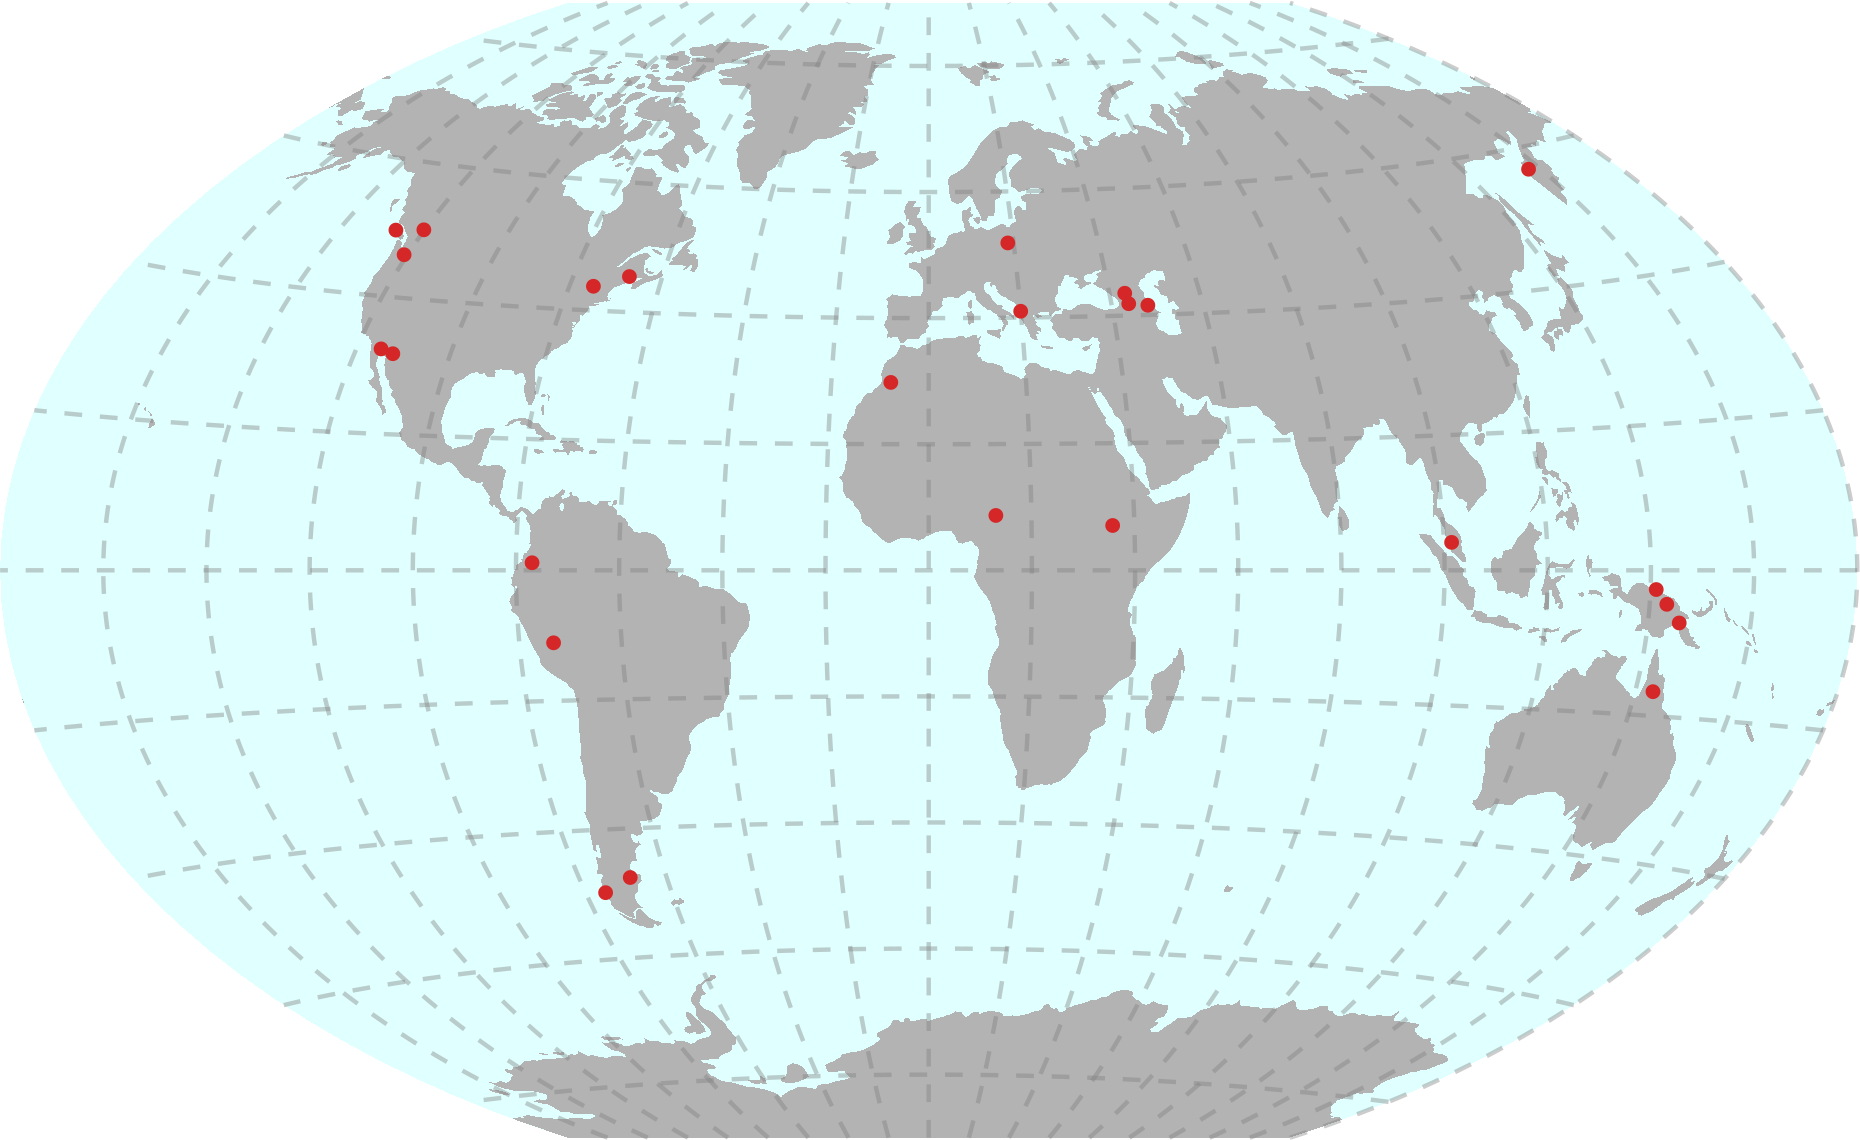
\includegraphics[width=\textwidth]{figures/fig81.png}
\caption{\label{fig:8.1}Geographical distribution of languages in Highly Complex portion of sample.}
\end{figure}

  In \figref{fig:8.1}, there are the expected clusters of languages in the Pacific Northwest and Caucasus regions. Smaller clusters of unrelated languages include: \ili{Tohono O’odham} and \ili{Cocopa} in the Sonoran Desert region, \ili{Passamaquoddy-Maliseet} and \ili{Mohawk} in the northeastern region of the USA and Canada, and \ili{Qawasqar} and \ili{Tehuelche} in Patagonia. Even three of the languages with Highly Complex syllable structure as a minor pattern -- \ili{Alamblak}, \ili{Menya}, and \ili{Wutung} -- are found in relative geographic proximity to one another in New Guinea. In most of these regions, there is historical and linguistic evidence of long-term cultural contact among unrelated ethnolinguistic groups. For example, while \ili{Tohono O’odham} and \ili{Cocopa} are not known to have been in intensive direct contact with each other, recall the discussion from \sectref{sec:8.4.3} noting that languages from the Tepiman branch of Uto-Aztecan and those of the Yuman family are known to have a long history of contact. 

  In a few cases, the evidence suggests that phonological patterns of languages in the sample have changed in the context of language contact. As mentioned in \sectref{sec:8.4.3}, \ili{Lelepa} is known to be in direct contact with other languages with similarly complex syllable patterns. In the preface to a volume titled \textit{Angan Languages Are Different}, \citet[4]{Healey1981} writes that the Angan language family to which \ili{Menya} belongs is “characterized by phonological complexity unusual in this country”. Wurm and colleagues remark on the “aberrant” nature of Angan languages within the Trans-New Guinea context and suggest that the characteristics of this small family suggest a “strong super-imposition upon an older, probably unrelated language type” (\citeyear{WurmEtAl1977}: 310). This seems to imply a contact or substrate origin for some of the phonological differences that Angan languages exhibit.

  That syllable structure complexity has been described as a feature of linguistic areas known for their diversity such as the Pacific Northwest and the Caucasus suggests that such patterns can spread from one language to another in situations of heavy language contact and bi- or multilingualism. Yet we know from observations of loanword adaptation that novel syllable structures are not easily borrowed; one of the major crosslinguistic loci of epenthesis processes is precisely in this context \citep{Hall2011}. This raises the question of how syllable patterns, especially highly complex ones that are crosslinguistically rare to begin with, converge in languages in situations of contact.

  It has been noted that in situations of language contact, prosodic and suprasegmental phenomena are more likely to diffuse than phonemes (chapters in \citealt{AikhenvaldDixon2001b}). There is a growing body of empirical evidence for this observation. \citet{Mennen2004} found that \ili{Dutch}-\ili{Greek} bilinguals who acquired \ili{Greek} in adulthood transferred peak alignment patterns from \ili{Dutch} into their \ili{Greek} speech. Native speakers of \ili{Tswana} were found not to apply phrase-final lengthening in their \ili{English} speech, in accordance with their L1 patterns, setting the intonational properties of their speech apart from those of South African \ili{English} and \ili{Afrikaans} \ili{English} speakers (\citealt{CoetzeeWissing2007}). \citet{Simonet2011} reports that \ili{Spanish}-Majorcan \ili{Catalan} bilinguals tend to transfer utterance-final pitch accents from their L1 to their L2. In a study of \ili{English}-Mexican \ili{Spanish} bilinguals in Los Angeles, \citet{Robles-Puente2014} found that both speakers who had moved to Los Angeles in childhood and those who had been born in Los Angeles to immigrant parents retained Mexican \ili{Spanish} intonational contours in their \ili{Spanish} and \ili{English} speech.

  As discussed in previous chapters, the component of speech prosody which has been most often associated with syllable complexity is speech rhythm. Instrumental investigations providing evidence for the influence of L1 rhythmic patterns on L2 (and sometimes vice versa) are becoming more prevalent in the literature. \citet{WhiteMattys2007} measured acoustic correlates of rhythm in native and non-native \ili{English}, \ili{Dutch}, \ili{Spanish}, and \ili{French} speech. They found that L1 has an effect on L2 which is observable in the rhythm metrics VarcoV (standard deviation of vocalic interval duration divided by the mean vocalic duration) and \%V (proportion of vocalic intervals). In L2 speech, the values for these metrics usually fell somewhere between the values measured for native speech in each of the languages. A comparison of the Pairwise Variability Index (PVI) metric in the speech of \ili{Spanish} monolinguals and speakers of Hispanic \ili{English} revealed a \ili{Spanish} substrate influence on the speech of the latter \citep{Carter2005}. Further, the rhythmic properties of Hispanic \ili{English} were found to be quite uniform across speakers regardless of generation, which the author suggests may be indicative of long-term persistence of  the substrate influence. \citet{Robles-Puente2014} found that \ili{English}-\ili{Spanish} bilinguals who had been in Los Angeles since childhood or were raised there by immigrant parents showed \ili{Spanish}-like rhythm in both languages. Finally, the effect may go the other way as well: \ili{Afrikaans}-\ili{Spanish} bilinguals who had been living in a \ili{Spanish}-dominant environment (in Patagonia) for at least two-thirds of their lives were found to show more \ili{Spanish}-like values for the nPVI-V metric in their \ili{Afrikaans} speech than non-bilingual \ili{Afrikaans} speakers \citep{CoetzeeEtAl2015}. 

  Because the rhythm metrics mentioned in the research above correspond to durational properties of consonant and vowel intervals, they may reflect timing patterns which relate directly to syllable structure complexity. There is at least one case in which the instrumentally-confirmed rhythmic properties of a language correspond to a historically documented process of contact-induced syllable structure change. This is the case of Moroccan \ili{Arabic}.

  Dialects of \ili{Arabic} spoken in North Africa, also known as Western \ili{Arabic}, have often been said to have phonetic and rhythmic properties which differ markedly from those of the dialects spoken in the Middle East (Eastern \ili{Arabic} dialects). In a perceptual experiment, native speakers of various dialects of \ili{Arabic} were able to correctly identify \ili{Arabic} speakers as coming from North Africa or the Middle East 98\% of the time \citep{BarkatEtAl1999}. In this task, speakers mentioned that the perceptual characteristics of Western \ili{Arabic} which helped them make this identification were that it sounded “faster” than Eastern \ili{Arabic} and had a “jerky” or “halting” sound \citep{GhazaliEtAl2002}. All varieties of \ili{Arabic} have been described as stress-timed in the literature; however, the salient perceptual differences between Western and Eastern \ili{Arabic} have prompted instrumental investigations into the nature of rhythmic timing in the various dialects. An analysis of the acoustic properties of Western (specifically Moroccan, Algerian, and Tunisian) and Eastern (specifically Egyptian, Jordanian, and Syrian) dialects of \ili{Arabic} revealed extreme differences in their values for metrics used to quantify speech rhythm properties \citep{HamdiEtAl2004}. Western \ili{Arabic} dialects had values for ΔC (standard deviation in consonant intervals) and \%V (proportion of vocalic intervals) which were even more extreme than those found for the ``prototypical'' stress-timed language \ili{English}. The ΔC and \%V values for Eastern \ili{Arabic} dialects put these languages closer to \ili{French}, which is said to have syllable timing. Of the three Western \ili{Arabic} dialects, Moroccan \ili{Arabic} had the most extreme high ΔC and low \%V values. The authors attributed this pattern to the frequent deletion of short vowels in this dialect, which creates consonant clusters and syllabic consonants, and also to the generally shorter duration noted for both phonologically long and short vowels in this dialect as compared to Eastern \ili{Arabic} dialects.

  \citet{Chtatou1997} notes that the phonetics, phonology, morphology, and lexicon of Moroccan \ili{Arabic} have been heavily influenced by contact with the \ili{Amazigh} (Berber) languages indigenous to the region, including \ili{Tamazight}, Tarifit, and \ili{Tashlhiyt}, with influences being likened to heavy substrate effects. In the most recently Arabized regions, Moroccan \ili{Arabic} may be so phonetically different from other Western dialects of \ili{Arabic} that speakers of the other dialects have trouble understanding it (Ibid. 105). Some of the phonetic differences can be attributed to patterns of vowel reduction resulting in complex consonant clusters. Recall from previous examples that \ili{Tashlhiyt} has highly complex syllable structure due to the prevalence of syllabic consonants in the language, which frequently result in long word-marginal strings of consonants or even words without vowels. In accordance with the phonetic patterns of local \ili{Amazigh} dialects, Moroccan \ili{Arabic} varieties are characterized by rampant vowel reduction resulting in tautosyllabic clusters or syllabic consonants, depending on the analysis. This is apparent when comparing Classical \ili{Arabic} (CA) forms to their Moroccan \ili{Arabic} (MA) equivalents: e.g. CA /na.di.ma/ > MA /n.dm/ ‘to regret;’ CA /ta.qaː.ba.la/ > MA /t.qaː.bl/ ‘to meet’ \citep[110]{Chtatou1997}. We see from comparison with Eastern dialects of \ili{Arabic} that this pattern is unique to Moroccan \ili{Arabic}. Other dialects have kept most of the vowels of Classical \ili{Arabic}, though vowel quality changes may have occurred \REF{ex:8.5}:

\ea\label{ex:8.5}
  Comparison of forms in Classical \ili{Arabic}, Eastern dialects, and Moroccan \ili{Arabic}

  CA \textit{katabtu} > Egyptian \ili{Arabic} \textit{katabt} > MA \textit{ktbt} ‘I wrote’ 

  CA \textit{taktubu} > Saudi \ili{Arabic} \textit{tiktib} > MA \textit{ka tktb} ‘you (\textsc{m}) write’

  CA \textit{taskunu} > Iraqi \ili{Arabic} \textit{tiskin} > MA \textit{ka tskn} ‘you (\textsc{m}) live’
\citep[111--112]{Chtatou1997}
\z

This pattern of vowel deletion is extremely productive and applied quite generally to loanwords. The most common pattern in syllable structure adaptation in lexical items from Classical \ili{Arabic} is the deletion of short vowels and the preservation of long ones, as in the word for ‘to meet’ given above. Similar patterns may be observed in the adaptation of \ili{French} loanwords into Moroccan \ili{Arabic}: e.g. Fr. \textit{direction} > MA \textit{drksjuːn} ‘direction;’ Fr. \textit{tracteur} > MA \textit{trktu}ː\textit{r} ‘tractor’ (\citealt[116]{Chtatou1997}; note that the final prosodically prominent vowel has been retained). \citet{Sayahi2005} describes a number of patterns by which vowel-initial \ili{Spanish} loanwords into Moroccan \ili{Arabic} are made to have more complex syllable structure: e.g. Sp. \textit{equipo} > MA \textit{lkipo} ‘team;’ Sp. \textit{espia} > MA \textit{spia} ‘spy;’ Sp. \textit{enfermero} > MA \textit{frmiro} ‘nurse.’

  The phenomenon described above is quite interesting, because reported instances of nativization of syllable patterns in the literature tend to involve the simplification of patterns; e.g. \ili{English} \textit{technostress} > \ili{Japanese} \textit{tekunosutoresu} \citep[69]{Kay1995}. Similarly, when languages with complex syllable structure borrow words from languages with simpler syllable structure, segmental patterns are often nativized, but syllable patterns are usually retained; e.g. \ili{Japanese} \textit{tsunami} [t͡sɯnami] > \ili{English} [su]\textit{nami}; \ili{English} \textit{Hamlet} > \ili{Russian} [ɡ]\textit{am}[lʲ]\textit{et}. Both Moroccan \ili{Arabic} and \ili{Amazigh} varieties have phonological words which are similar in shape to the Classical \ili{Arabic}, \ili{French}, and \ili{Spanish} source words given above; e.g. \ili{Tashlhiyt} \textit{tifunasin} ‘cows,’ Moroccan \ili{Arabic} \textit{hadak} ‘\textsc{dem.}’ Thus it is not readily apparent why loanwords would be borrowed in such a way as to create such complex onsets. This is a case in which morphosyntactic patterns of the language may have some effect on the phonological adaptation of loanwords. In Moroccan \ili{Arabic}, as in \ili{Tashlhiyt}, the inflectional morphology of the language relies in part on nonconcatenative processes which can be lexically determined and dependent upon the phonological form of words, many of which have complex clusters and also tend to be monosyllabic \citep{Heath2007}. Perhaps loanword adaptation is in part affected by analogy to such patterns. Nevertheless, as we know from the historical and comparative evidence, those very patterns originated in highly productive patterns of vowel reduction which were carried over from \ili{Amazigh}.

  The case of Moroccan \ili{Arabic} suggests that native properties of speech rhythm, including vowel reduction and tendencies toward longer consonant intervals and shorter vowel intervals in speech, may be transferred by speakers to an L2 much in the same way that intonational contours are transferred. In situations of intense cultural contact and high rates of bilingualism and multilingualism, it is easy to imagine rhythmic properties being transferred in this way among unrelated languages with the effect that similar syllable patterns may be found in them.

\subsection{Development of Highly Complex syllable structure: Conclusions and questions}\label{sec:8.4.6}

  Syllable structure has long been known to become more complex through processes of vowel reduction. The associations between syllable complexity and other phonetic, phonological, and morphological properties suggest that the path to highly complex syllable structure additionally tends to include other specific processes and properties in addition to vowel reduction or deletion.

  It is clear from the crosslinguistic trends, the comparison of related pairs of languages, and the case study of \ili{Lezgian} that stress-conditioned vowel reduction, in particular, is almost always relevant in the development of highly complex syllable structure. The findings here also point to the persistence and increasing prevalence of vowel reduction as syllable structure becomes more complex. Morphologically complex contexts are more often than not a factor, though the \ili{Lezgian} example shows that this does not always have to be the case.

  Consonant inventory size is additionally strongly associated with syllable complexity, and specific consonantal articulations with either end of the syllable complexity scale. However, the crosslinguistic patterns in specific segmental contrasts were not strongly upheld in the comparisons of related languages. The comparisons of related pairs of languages largely showed the expected patterns with respect to a higher prevalence of consonant allophony in the languages with simpler syllable patterns, but in the \ili{Lezgian} example, place assimilation of consonants to vowels occurs concurrently with, or shortly following, vowel reduction. Perhaps the inconsistent patterns with respect to consonantal articulations and consonant-affecting processes are related to the speed with which vowel reduction affects syllable structure patterns, or even the specific kind of vowel reduction operating within a language (e.g. quality, devoicing, reduction in duration). That is, the same underlying mechanisms for vowel reduction may also condition consonant processes that lead to larger inventories, albeit in complex and varied ways. Without detailed historical accounts, it is difficult to identify the specific patterns that consonant changes may take as part of a larger process of syllable structure change. However, the consistent differences in consonant phoneme inventory size in languages with simpler and more complex syllable structure suggest that there is a non-coincidental relationship there.

  Another important consideration in the development of highly complex syllable structure is the issue of contact and transfer of rhythmic properties from one language to another. It is not clear whether we should expect many correlates of highly complex syllable structure to occur when syllable complexity is increased as a result of rhythmic transfer from one language to another in situations of intense contact. Perhaps this is another case where segmental, allophonic, and even morphological patterns may deviate from the predictions derived from the crosslinguistic patterns.

  A question that still remains open is how, specifically, the diachronic path leading to highly complex syllable structure gets started in a language. In light of the findings and discussions above, I have one specific hypothesis which is based on observations of vowel reduction patterns in languages with Simple syllable structure. Recall from the summary of vowel reduction processes in \sectref{sec:6.3.6} that the most common process type in the Simple category is the devoicing of vowels at word or phrase/utterance margins. In the comparison of pairs in \sectref{sec:8.4.3}, 3/4 languages with the simpler syllable patterns (\ili{Ute}, \ili{Apurinã}, and \ili{Maori}) have vowel devoicing as an outcome of vowel reduction. This proportion, though derived from a tiny group of languages, is larger than the overall proportion of languages in the Simple category which have devoicing as an outcome of vowel reduction (6/13). That is, in language families in which both extreme syllable patterns occur, such that there is the phonological and morphological potential for languages with simpler syllable patterns to follow a similar path as their relatives with more complex phonotactics, devoicing is very likely to be an outcome of vowel reduction in the languages with simpler patterns. This is interesting, because vowel reduction resulting in devoicing may be a more likely source of incipient syllable structure change than other forms of reduction. This is because devoiced vowels, especially in domain-marginal contexts, may be easily lost or restructured as glottal fricatives or aspiration. In \ili{Apurinã}, it has been noted that stops become aspirated preceding a devoiced unstressed vowel \REF{ex:8.6}.

\ea\label{ex:8.6}
  \etriple{Apurinã}{Arawakan}{Brazil}

/kaˈjati/

[kaˈjatʰi̥]\\
\glt ‘paca (large rodent)’
\citep[60--61]{Facundes2000} 
\z

  The \ili{Apurinã} example suggests that the properties of the devoiced vowel are becoming associated with the consonant, providing an ideal context for sound change, and in this case, syllable structure change.\footnote{{On the other hand, the aspiration analysis may simply be another way of noting the devoiced vowel.}} As described in \sectref{sec:3.2.3}, a similar process of vowel devoicing in \ili{Ute} has already affected the syllable patterns in that language. If domain-marginal vowel devoicing occurs in a language with word stress, perhaps such devoicing processes could disrupt the rhythmic patterns of the language, leading eventually to a stronger role of stress and associated segmental effects. This topic would be a good avenue for further research.

  In \figref{fig:8.2} I show how highly complex syllable structure and its associated properties might develop out of simpler syllable structure and its properties, according to the findings here.

\begin{sidewaysfigure}
\begin{tikzpicture}[>=Triangle,baseline]
\graph [branch down=7\baselineskip,grow right sep=1cm,nodes={font=\small,draw,rounded corners=2pt,text width=3.1cm,align=left}] {
a[as={stress-conditioned allophonic C processes}] -> {b[as={phonologiza\-tion of fortition, assimilation processes}] -> d[as={palato-alveolar, uvular, affricate, ejective phonemes}], c[xshift=-1.625cm,as={phonologiza\-tion of lenition processes, phonemicization of associated articulations}]};
e[as={domain-conditioned V devoicing},text width=3cm] ->[dashed] f[as={\itshape destabilization of stress patterns?},draw=none,text width=3.1cm] ->[dashed] {g[as={stress-conditioned V reduction, deletion},text width=3cm],h[as={syllabic Cs},yshift=3\baselineskip,align=center]} -> i[as={increased V reduction},text width=3.2cm] <- j[xshift=-4.475cm,yshift=-5\baselineskip,draw=none,as={\itshape stronger effects when morpheme/word ratio high, grammatical morphemes involved?},text width=3.2cm];
};
\draw[thick,-{Triangle[]}] (current bounding box.north west) ++(0,\baselineskip) -- (current bounding box.north east) node[above,at start,anchor=south west] {Simple} node[above,at end,anchor=south east] {Highly Complex};
\end{tikzpicture}
\caption{\label{fig:8.2}Proposed path of development for highly complex syllable structure out of simpler syllable patterns.}
\end{sidewaysfigure}


  In the discussions above I explored how highly complex syllable structure might arise over time in special phonological, morphological, and even sociolinguistic contexts. While there are still open questions regarding the details of these paths, I believe that the evidence shows that the processes involved are quite natural and common patterns of language change, a fact that stands in stark contrast to the frequent description of highly complex structures as marked or dispreferred. In the following section I discuss the long-term stability of these structures.

\section{Highly complex syllable structure: A stable and motivated pattern}\label{sec:8.5}

  Recall from the discussion of the literature in \chapref{sec:1} that many of the properties of highly complex syllable structure -- the size and composition of clusters, the presence of syllabic obstruents, its association with morphological complexity -- are crosslinguistically rare and/or theoretically problematic. Abstract theoretical accounts for the structures rarely touch upon practical aspects of these ``dispreferred'' patterns such as their maintenance and stability in speech communities in the long term. I discuss some of these issues here.

\subsection{Synchronic stability of Highly Complex syllable structure}\label{sec:8.5.1}

  In \chapref{sec:6} it was found that 21/25 of the languages in the Highly Complex category were reported to have processes of vowel reduction. The 15 languages in this category with stress-conditioned vowel reduction had on average three such processes as ongoing synchronic patterns. Altogether, processes of vowel deletion or reduction were found to alter syllable patterns in 13 of the languages in this category, either by turning onsets into codas, producing tautosyllabic clusters, or producing syllabic consonants. As mentioned in that chapter, what the crosslinguistic data suggests is that vowel reduction has the strongest effects on syllable structure in languages in which such processes have previously altered the canonical syllable patterns.

  Because highly complex syllable patterns are so crosslinguistically rare and ``dispreferred,'' we might expect to see in these languages more instances of simplification of syllable patterns than instances of syllable structure becoming more complex. As the discussion of directionality in \sectref{sec:8.4.1} suggests, this does not seem to be the case. In that discussion, I mentioned incipient processes of variable epenthesis and historical processes of cluster simplification. Here I present additional information regarding the stability of highly complex syllable structure by discussing regular (phonologized) processes of epenthesis and active processes of cluster simplification.

  An analysis of the languages in the Highly Complex category revealed that nine languages have regular phonological processes of epenthesis which break up consonant clusters. There are two kinds of epenthesis patterns which are characteristic of the languages of this group: processes which break up sequences of sounds which are identical or highly similar (e.g. sequences of sibilants), and processes which break up sequences of two sonorants or a sonorant and obstruent. I give an example of the latter process type in \REF{ex:8.7}.

\ea\label{ex:8.7}
  \etriple{Yakima Sahaptin}{Sahaptian}{USA}

\ea  /ʔínm/\\\relax
  [ʔínɨm]\\
  \glt ‘excessively’

\ex  /t͡ɬ’jálm/\\\relax
  [t͡ɬ’jálɨm]\\
  \glt ‘Cle Elum (place name)’

\ex  /talújm/\\\relax
  [talújɨm]\\
  \glt ‘nail’
\z
(\citealt[28]{HargusBeavert2006})
\z

Similar processes can also be found in \ili{Kabardian} and \ili{Doyayo}, among others. What is interesting about such patterns is that they do not target the long sequences of obstruents which are prototypical of highly complex syllable structure.

  An analysis of active (variable) processes of consonant deletion resulting in cluster simplification turned up similar results. There are ten languages with such patterns. Interestingly, such processes typically affect sonorants or glottal fricatives in these languages. While the affected sound in the example in \REF{ex:8.8} is transcribed as a voiced fricative, it patterns phonotactically with sonorants in \ili{Georgian} (\citealt{ShostedChikovani2006}: 261).

\ea\label{ex:8.8}
  \etriple{Georgian}{Kartvelian}{Georgia}

/vpɾt͡skʰvni/

[ɸpɾt͡skʰvni] {\textasciitilde} [pɾt͡skʰvni]\\
\glt ‘I peel’

(\citealt{ShostedChikovani2006}: 261)\footnote{{Elsewhere in this book I have followed \citet{Aronson1991} in transcribing the voiced labial fricative of \ili{Georgian} as bilabial /β/; however, some researchers classify it as a labiodental /v/. I use /v/ in this example to preserve Shosted \& Chikovani’s transcription.}}
\z

Again, the prototypical syllable patterns of these languages are not strongly affected by such processes. It should also be noted that four of the languages with processes like these have Highly Complex structures as a minor pattern (\ili{Alamblak}, \ili{Kunjen}, \ili{Menya}, and \ili{Wutung}).

  The distribution of processes of epenthesis and consonant deletion, as compared to the distribution of vowel reduction processes, suggests that despite theoretical issues of analysis, highly complex syllable structure is neither problematic for speakers, nor synchronically unstable in speech communities. The phonetic processes responsible for creating these syllable patterns appear to be both remarkably persistent and more prevalent than processes which ``repair'' them, at least in languages which have Highly Complex syllable structure as a prevalent pattern.

\subsection{Diachronic stability of syllable complexity}\label{sec:8.5.2}

  Complex syllable structure may show long-term stability within language families and regions. This is apparent in examining the geographical distribution of maximal syllable structure patterns. In constructing the language sample for the current study, it was impossible to find the Simple pattern within Eurasia, and very difficult to find such patterns in North America, such that 2/3 languages from this region in the Simple portion of the sample actually have Moderately Complex patterns. If we assume that the complex syllable patterns of these regions developed at some point out of simpler patterns, then the geographical distributions suggest that, once it develops, syllable complexity tends to persist for long periods of time. Similarly, a recent study of maximal syllable shapes in four proposed linguistic areas found that the patterns were more closely associated with language families than with regions, though there was limited evidence for convergence in parts of the Caucasus and Pacific Northwest (\citealt{NapoleãodeSouza2017}). The author’s interpretation of the findings was that syllable structure patterns may be a generally stable phonological property of languages, persisting for long periods of time within language families. If one considers only the universal preference for CV structures, these distributional facts are unexpected. We might expect that strong cognitive or physiological pressures favoring CV over all other syllable types would manifest crosslinguistically in such a way that languages with canonical (C)V patterns could be found in any language family or region.

  From a diachronic point of view, the observed patterns may relate to the way that vowel reduction, vowel epenthesis, and consonant deletion tend to operate within languages. Vowel deletion may cause canonical syllable patterns to change from fairly simple to quite complex in a relatively short period of time, such that a language which previously had only simple onsets may, just a few generations later, have a wide variety of highly complex clusters (e.g. \ili{Lezgian}). The opposite scenario, in which highly complex syllable patterns in a language are uniformly simplified by epenthesis in a short period of time, seems very unlikely. Crosslinguistically, epenthesis processes tend to target specific phonotactic environments or sequences of sounds \citep{Hall2011}. While such processes might simplify some specific syllable shapes in a language, they might leave many others unaffected, such that the overall syllable pattern of the language is still complex (cf. the \ili{Yakima Sahaptin} example in 8.7). Unless vowel epenthesis becomes a completely general process, or occurs in multiple iterations with different consonant sequences (both of which seem unlikely given crosslinguistic patterns), it is hard to imagine such a process dramatically changing the syllable patterns of a language in a short period of time. This also seems unlikely from an articulatory point of view, given that the widespread temporal adjustments to gestural organization required of such a scenario would run against general tendencies towards increased overlap and reduction of gestures (\citealt{BrowmanGoldstein1992b}). Similarly, processes of cluster reduction, as noted above, often target specific sequences, and it is hard to imagine these operating so generally as to obliterate both word-marginal and word-internal clusters in a language to the point where they dramatically affect canonical syllable patterns. 

  It seems that in the case of syllable structure, a high degree of complexity may be introduced quite rapidly into the system, but once there, it is difficult to completely remove. Historical processes suggest this is the case. In the Middle \ili{English} (ME) period, a series of vowel epenthesis processes targeted certain consonant sequences in the language which had been present in Old \ili{English} (OE): e.g. OE \textit{niht} > ME \textit{nyhyt} ‘night;’ OE \textit{myln} > ME \textit{milne} ‘mill’ (\citealt{Jones1989}: 167, 170). Similarly, some codas were lost through sonorization processes: e.g. West Saxon OE \textit{he\={} ɡ} > ME \textit{hei} ‘hay’ (Ibid. 150). Meanwhile, cluster simplification processes reduced /kn/ and /gn/ onsets \citep{Minkova2003}. Despite these changes to syllable patterns, which were quite widespread judging from orthographic evidence, onset clusters such as /pl/ and /fr/, and codas such as /nd/, were not affected by such processes: cf. OE \textit{ploga} ‘plough,’ OE \textit{fre}\textsf{\={} }\textit{ond} ‘friend.’ Thus while syllable complexity was simplified at the level of specific sequences in the language, and simple syllable shapes perhaps became more frequent, the canonical syllable patterns of the language were not strongly affected. By comparison, later processes of vowel deletion added considerably to the complexity of coda patterns in the language, yielding what are today the maximal tautosyllabic clusters in the language: \textit{si}[ksθs], \textit{te}[ksts], and so on.

\subsection{Phonetic properties of Highly Complex syllable patterns and long-term stability}\label{sec:8.5.3}

  Researchers often remark upon the salient phonetic characteristics of highly complex syllable patterns. In \sectref{sec:3.4.3} I presented a variety of phonetic descriptions of consonant (usually obstruent) clusters in languages from the Highly Complex portion of the sample. The accounts describe the clusters in these languages as being characterized by ``open transition,'' ``transitional vocoids,'' ``overtones,'' ``strong aspirated release,'' ``audible intervals,'' and so on. These phonetic properties are described for sequences analyzed as clusters and those analyzed as syllabic obstruents, and all share properties typical of intrusive vowels as defined by \citet{Hall2006}. In my previous discussion of these patterns, I concluded that such transitions are a prominent characteristic of Highly Complex syllable structure and constitute a phonetic correlate of this language type. I propose that these salient phonetic characteristics, which derive from temporal properties of gestural organization, facilitate the long-term maintenance and stability of highly complex syllable patterns which most models of the syllable predict to be dispreferred.

  There is a small body of research which relates the temporal properties of gestural organization of obstruent sequences to perceptual recoverability. Consonant clusters have been found to be characterized by less overlap between gestures when occurring in word-initial position than in other positions (cf. \citealt{Byrd1996a} for \ili{English}). In a perceptual recoverability account, word-initial position may correspond to utterance-initial position in discourse. If a word-initial sequence of obstruents, especially stops, occurs in utterance-initial position, there is no vowel preceding the first consonant which could provide acoustic cues as to its place of articulation. A release of the first stop would cue acoustic information on its place of articulation, while heavy overlap with the following consonant would obscure such acoustic cues. Perception of the first stop would be additionally facilitated if a vocalic transition is present, since this allows for a greater distribution of acoustic cues in time (\citealt{RidouaneFougeron2011}: 294). In this view, gestural organization strategies resulting in a temporal lag between word-initial obstruents may have a perceptual motivation; that is, overlap between consonant gestures may be suppressed in order to preserve phonetic cues.

  Perceptual recoverability has been suggested as a motivation behind timing patterns observed in clusters in \ili{Korean} (\citealt{SilvermanJun1994}), Tsou \citep{Wright1996}, \ili{Georgian} \citep{ChitoranEtAl2002}, and \ili{Tashlhiyt} (\citealt{RidouaneFougeron2011}). Some of these studies have shown that it is not just word onset position, but also the relative place of articulation of the consonants in sequence which contribute to observed temporal lag, which somewhat weakens the original argument for perceptual recoverability. Indeed, most of the phonetic descriptions of highly complex clusters in \sectref{sec:3.4.3} do not refer specifically to word-initial or even onset environments, but instead mention specific sequences of consonants. In \ili{Cocopa}, for example, transitional elements can be found in at least some word-final consonant sequences \REF{ex:8.9}.

\ea\label{ex:8.9}
  \etriple{Cocopa}{Cochimi-Yuman}{USA}

k\textsuperscript{a}myúx\textsuperscript{i}ɬʲ\\
\glt ‘I hope that somehow you will’
\citep[47]{Crawford1966}
\z

Additionally, \citet{ChitoranCohn2009} note that in \ili{Georgian} onsets, the timing lag between consonant gestures is larger than what is needed for the release burst to be perceptually recoverable. They further suggest that timing differences between consonant sequences in \ili{Georgian} reflect phonologized patterns of language-specific gestural organization.

  Considering that obstruent clusters in languages with highly complex syllable structure come about through vowel reduction, and that place characteristics of the original vowel may be retained in release bursts (cf. descriptions of clusters in \ili{Lezgian} and \ili{Tohono O’odham} in \sectref{sec:3.4.3}), it seems more likely that perceptual recoverability is an effect of, rather than a motivation for, the gestural organization of clusters in these languages. I suggest that the gestural timing and perceptual properties of such sequences may facilitate the long-term maintenance of highly complex syllable patterns by making them less susceptible to complete overlap resulting in consonant deletion (\citealt{BrowmanGoldstein1990}).

\section{Topics for further research}\label{sec:8.6}

  In this book I have shown that highly complex syllable structure is a holistic linguistic type associated with a number of phonetic, phonological, and morphological correlates. Additionally, the crosslinguistic patterns identified here may point to general tendencies in the diachronic development of these structures. However, there are many ways in which the studies here can be expanded. Some of the results also suggest lines of research outside of the range of standard phonological typology.

  An issue which should be explored in more depth is that of the type frequency of syllable patterns. This issue was touched upon only briefly in the discussion of the prevalence of highly complex patterns in \chapref{sec:3}. A finer-grained analysis of frequency patterns may refine our understanding of how processes of vowel reduction and consonant allophony work their way through the language as syllable structure changes. Similarly, the treatment of morphology was necessarily brief and general in the current study, but there is ample ground for further research here. Relevant topics may include the type (e.g. prefixing, suffixing, infixing, templatic, etc.) and function (inflection, compounding, lexical class-changing derivation, lexical affixation, etc.) of morphological patterns which occur in tautosyllabic clusters of different degrees of complexity. Additionally, it would be interesting to establish a crosslinguistic range for the distribution of morphologically simple and complex tautosyllabic clusters or syllable inventories, as the results here point to a great deal of variation with respect to such distributions even within the Highly Complex portion of the sample. Though such studies have been conducted for a handful of European languages (\citealt{DresslerDziubalska-Kołaczyk2006}, \citealt{DresslerEtAl2010}, inter alia), a truly global examination of these issues could better inform our understanding of the development of phonotactic complexity. A preliminary investigation in this vein suggests that at least for onsets, morphologically complex consonant clusters are more restricted in their structure and distribution than morpheme-internal clusters in a variety of ways \citep{Easterday2019}.

  Another issue which deserves more attention is that of language contact and syllable structure complexity. While linguistic areas such as the Pacific Northwest and the Caucasus region are well known for unusual syllable complexity, possibly as an effect of contact, some patterns noted above suggest that this phenomenon may be relatively frequent at an even smaller scale. The situation of \ili{Lelepa} and its neighbors is especially striking because it shows emerging complexity at a very local level in a situation of contact, but within a larger family which is famous for its simple syllable patterns (Oceanic). A global survey of similar small-scale clusters of syllable patterns may reveal important information about the role of contact in the development of phonological complexity.

  Finally, the results of the current study suggest that there are properties of gestural organization associated with both synchronic characteristics of highly complex syllable patterns and diachronic stages of their development. Synchronically, the obstruent clusters associated with these syllable patterns are characterized by open transitions between consonantal gestures which may in many cases have their source in processes of vowel reduction. Diachronically, the contrastive consonant articulations associated with these languages may originate in patterns of increased overlap of consonantal and vocalic gestures and strengthening of consonantal gestures at some point in the history of these languages, perhaps even before the development of complex syllable patterns. There is a growing literature of instrumental investigations of gestural organization in the syllable patterns of diverse languages. Many of these studies are relevant to the issues examined here concerning properties of consonant clusters (cf. \citealt{GoldsteinEtAl2007} for \ili{Georgian} and \ili{Tashlhiyt}, \citealt{HermesEtAl2013} for \ili{Italian}, \citealt{Marin2014} for \ili{Romanian}, \citealt{Butler2015} for \ili{Khmer} and \ili{Bunong}, \citealt{MarinEtAl2017} for seven European languages) and syllabic consonants (cf. \citealt{HermesEtAl2011} for \ili{Tashlhiyt}, \citealt{PouplierBeňuš2011} for \ili{Slovak}). The findings in the current study reveal a prevalence of vowel reduction in languages with more complex syllable patterns and suggest a prevalence of coarticulation of consonants with adjacent vowels and strengthening in languages with simpler syllable patterns. In light of these findings, it would be interesting to instrumentally investigate general patterns of gestural organization as they pertain to those specific issues in languages with differing syllable complexity.
  

% 

\subsection{Appendix A: Language sample}
\begin{styleBody}
Information on the language sample used in the study is listed in Tables A1-A4.
\end{styleBody}

\begin{styleBody}
\textbf{\textsc{Key} \textbf{to} \textbf{reading} \textbf{table:}}
\end{styleBody}

\begin{styleBody}
\textbf{ISO} \textbf{693-3:} ISO 693-3 code for language used in survey.
\end{styleBody}

\begin{styleBody}
\textbf{Language:} Dialect is given in parentheses where relevant.
\end{styleBody}

\begin{styleBody}
\textbf{Syllable} \textbf{Structure:} 
\end{styleBody}

\begin{styleBody}
\textbf{\textit{S} }= Simple 
\end{styleBody}

\begin{styleBody}
\textbf{\textit{MC} }= Moderately Complex
\end{styleBody}

\begin{styleBody}
\textbf{\textit{C} }= Complex
\end{styleBody}

\begin{styleBody}
\textbf{\textit{HC} }= Highly Complex
\end{styleBody}

\begin{styleBody}
\textbf{Macro-area:} Following Dryer (1989: 268; 1992: 83, 133-5). 
\end{styleBody}

\begin{styleBody}
\textbf{\textit{Africa} \textit{=}} continent of Africa, including Semitic languages of southwest Asia. 
\end{styleBody}

\begin{styleBody}
\textbf{\textit{Australia} \textit{\&} \textit{New} \textit{Guinea} \textit{=}} Australian continent and Melanesia, excluding Austronesian languages of Melanesia. 
\end{styleBody}

\begin{styleBody}
\textbf{\textit{Eurasia} \textit{=}} Eurasian landmass, excluding Semitic and languages from families of southeast Asia as defined below, and including the Munda languages of Austro-Asiatic. 
\end{styleBody}

\begin{styleBody}
\textbf{\textit{North} \textit{America} \textit{=} }North American continent, including languages of Mexico, Mayan and Aztecan languages in Central America, and some branches of Chibchan-Paezan. 
\end{styleBody}

\begin{styleBody}
\textbf{\textit{South} \textit{America} \textit{=}} South American continent, including languages of Central America except Mayan and Aztecan languages, and some Chibchan-Paezan branches. 
\end{styleBody}

\begin{styleBody}
\textbf{\textit{Southeast} \textit{Asia} \textit{\&} \textit{Oceania} \textit{=} }Southeast Asian region, including all Sino-Tibetan, Tai-Kadai, Hmong-Mien, and Austro-Asiatic languages excluding Munda, and Oceania region (Austronesian languages).
\end{styleBody}

\begin{styleBody}
\textbf{Top-level} \textbf{family} and \textbf{Subfamily:} Following genealogical classifications listed in Glottolog 3.3 \citep{HammarströmEtAl2018}.
\end{styleBody}

\begin{styleBody}
\textbf{Speaker} \textbf{Population:} L1 speaker population figure for language (or specific dialect) given in Ethnologue 21 (\citealt{SimonsFennig2018}). An asterisk indicates that another source was used for population estimate; these can be found beneath the table.
\end{styleBody}

\begin{styleBody}
\textbf{Date:} Date given in Ethnologue 21 (\citealt{SimonsFennig2018}) for speaker population figure.
\end{styleBody}

\begin{styleBody}
\textbf{Vitality} \textbf{Status:} Following Ethnologue 21 (\citealt{SimonsFennig2018}). 
\end{styleBody}

\begin{styleBody}
\textbf{\textit{Institutional} \textit{=}} language has wide use in the home and community and official status at educational, provincial, national, and/or international levels. 
\end{styleBody}

\begin{styleBody}
\textbf{\textit{Developing} \textit{=}} language is used in the home, community, and sometimes broader contexts, and in initial stages of developing a system of writing and standardization. 
\end{styleBody}

\begin{styleBody}
\textbf{\textit{Vigorous} \textit{=}} language is used in the home and community by speakers of all generations, but has not yet developed a system of graphization or standardization. 
\end{styleBody}

\begin{styleBody}
\textbf{\textit{In} \textit{Trouble} \textit{=}} language is currently in the process of losing intergenerational transmission, with the community shifting to other languages for daily use, but there are still speakers of child-bearing age. 
\end{styleBody}

\begin{styleBody}
\textbf{\textit{Dying} \textit{=}} language has lost intergenerational transmission entirely, and all fluent speakers are above child-bearing age.
\end{styleBody}

\tablefirsthead{}

\tabletail{}
\tablelasttail{}
\begin{tabularx}{\textwidth}{XXXXXXXXX}
\lsptoprule

 \textbf{ISO} \textbf{639-3} & \textbf{Language} & \textbf{Syllable} \textbf{Structure} & \textbf{Macro-area} & \textbf{Top-level} \textbf{family} & \textbf{Subfamily} & \raggedleft \textbf{Speaker} \textbf{Population} & \textbf{Date} & { \textbf{Vitality}}

 \textbf{Status}\\
 hts & {\mdseries\upshape \textbf{Hadza}} & S & Africa & {\mdseries\upshape (isolate)} &  & \raggedleft 950 & 2013 & In Trouble\\
 grj & {\mdseries\upshape \textbf{Southern} \textbf{Grebo}} & S & Africa & {\mdseries\upshape Atlantic-Congo} & {\mdseries\upshape \textit{Volta-Congo}} & \raggedleft 65,000 & 2012 & Vigorous\\
 yor & {\mdseries\upshape \textbf{Yoruba}} & S & Africa & {\mdseries\upshape Atlantic-Congo} & {\mdseries\upshape \textit{Volta-Congo}} & \raggedleft 19,043,700 & 1993 & Institutional\\
 mhi & {\mdseries\upshape \textbf{Ma’di}} & S & Africa & {\mdseries\upshape Central Sudanic} & {\mdseries\upshape \textit{Moru-Madi}} & \raggedleft 293,000 & 2014 & Developing\\
 bbo & {\mdseries\upshape \textbf{Southern} \textbf{Bobo} \textbf{Madaré}} & S & Africa & {\mdseries\upshape Mande} & {\mdseries\upshape \textit{Western} \textit{Mande}} & \raggedleft 181,000 & 2009 & Developing\\
 svs & {\mdseries\upshape \textbf{Savosavo}} & S & Aus \& New Guinea & {\mdseries\upshape (isolate)} &  & \raggedleft 2,420 & 1999 & Vigorous\\
 kbk & {\mdseries\upshape \textbf{Grass} \textbf{Koiari}} & S & Aus \& New Guinea & {\mdseries\upshape Koiarian} & {\mdseries\upshape \textit{Koiaric}} & \raggedleft 1,700 & 2000 & Vigorous\\
 roo & {\mdseries\upshape \textbf{Rotokas}} & S & Aus \& New Guinea & {\mdseries\upshape North Bougainville} & {\mdseries\upshape \textit{Rotokas-Askopan}} & \raggedleft 4,320 & 1981 & Developing\\
 kjs & {\mdseries\upshape \textbf{East} \textbf{Kewa}} & S & Aus \& New Guinea & {\mdseries\upshape Nuclear Trans New Guinea} & {\mdseries\upshape \textit{Enga-Kewa-Huli}} & \raggedleft 45,000 & 2000 & Developing\\
 tow & {\mdseries\upshape \textbf{Towa}} & S & N America & {\mdseries\upshape Kiowa-Tanoan} &  & \raggedleft 1,790 & 2007 & In Trouble\\
 mio & {\mdseries\upshape \textbf{Pinotepa} \textbf{Mixtec}} & S & N America & {\mdseries\upshape Otomanguean} & {\mdseries\upshape \textit{Eastern} \textit{Otomanguean}} & \raggedleft 20,000 & 1990 & Vigorous\\
 ute & {\mdseries\upshape \textbf{Ute}} & S & N America & {\mdseries\upshape Uto-Aztecan} & {\mdseries\upshape \textit{Northern} \textit{Uto-Aztecan}} & \raggedleft 920 & 2007 & In Trouble\\
 ura & {\mdseries\upshape \textbf{Urarina}} & S & S America & {\mdseries\upshape (isolate)} &  & \raggedleft 3,000 & 2002 & Developing\\
 wba & {\mdseries\upshape \textbf{Warao}} & S & S America & {\mdseries\upshape (isolate)} &  & \raggedleft 28,100 & 2007 & Vigorous\\
 apu & {\mdseries\upshape \textbf{Apurinã}} & S & S America & {\mdseries\upshape Arawakan} & {\mdseries\upshape \textit{Southern} \textit{Maipuran}} & \raggedleft 2,870 & 2006 & In Trouble\\
 huu & {\mdseries\upshape \textbf{Murui} \textbf{Huitoto}} & S & S America & {\mdseries\upshape Huitotoan} & {\mdseries\upshape \textit{Nuclear} \textit{Witotoan}} & \raggedleft 2,000 & 2016 & In Trouble\\
 cav & {\mdseries\upshape \textbf{Cavineña}} & S & S America & {\mdseries\upshape Pano-Tacanan} & {\mdseries\upshape \textit{Tacanan}} & \raggedleft 600 & 2011 & In Trouble\\
 cub & {\mdseries\upshape \textbf{Cubeo}} & S & S America & {\mdseries\upshape Tucanoan} & {\mdseries\upshape \textit{Eastern} \textit{Tucanoan}} & \raggedleft 6,260 & 2008 & Institutional\\
 dru & {\mdseries\upshape \textbf{Rukai} \textbf{(Budai} \textbf{dialect)}} & S & SE Asia \& Oceania & {\mdseries\upshape Austronesian} &  & \raggedleft 10,500 & 2002 & Developing\\
 mri & {\mdseries\upshape \textbf{Maori}} & S & SE Asia \& Oceania & {\mdseries\upshape Austronesian} & {\mdseries\upshape \textit{Malayo-Polynesian}} & \raggedleft 158,640 & 2013 & In Trouble\\
 khc & {\mdseries\upshape \textbf{Tukang} \textbf{Besi} \textbf{North}} & S & SE Asia \& Oceania & {\mdseries\upshape Austronesian} & {\mdseries\upshape \textit{Malayo-Polynesian}} & \raggedleft 120,000 & 1995 & Vigorous\\
 sxr & {\mdseries\upshape \textbf{Saaroa}} & S & SE Asia \& Oceania & {\mdseries\upshape Austronesian} & {\mdseries\upshape \textit{Tsouic}} & \raggedleft 10 & 2012 & Dying\\
 iii & {\mdseries\upshape \textbf{Sichuan} \textbf{Yi}} & S & SE Asia \& Oceania & {\mdseries\upshape Sino-Tibetan} & {\mdseries\upshape \textit{Burmo-Qiangic}} & \raggedleft 2,000,000 & 2004 & Institutional\\
\lspbottomrule
\end{tabularx}
\begin{styleBody}
\textbf{Table} \textbf{A1.} Portion of language sample with Simple syllable structure.
\end{styleBody}

\tablefirsthead{}

\tabletail{}
\tablelasttail{}
\begin{tabularx}{\textwidth}{XXXXXXXXX}
\lsptoprule

 \textbf{ISO} \textbf{639-3} & \textbf{Language} & \textbf{Syllable} \textbf{Structure} & \textbf{Macro-area} & \textbf{Top-level} \textbf{family} & \textbf{Subfamily} & \raggedleft \textbf{Speaker} \textbf{Population} & \textbf{Date} & { \textbf{Vitality}}

 \textbf{Status}\\
 ktb & {\mdseries\upshape \textbf{Kambaata}} & MC & Africa & {\mdseries\upshape Afro-Asiatic} & {\mdseries\upshape \textit{Cushitic}} & \raggedleft 743,000 & 2007 & Institutional\\
 ewe & {\mdseries\upshape \textbf{Ewe}} & MC & Africa & {\mdseries\upshape Atlantic-Congo} & {\mdseries\upshape \textit{Volta-Congo}} & \raggedleft 4,184,000 & 2013 & Institutional\\
 fvr & {\mdseries\upshape \textbf{Fur}} & MC & Africa & {\mdseries\upshape Furan} &  & \raggedleft 745,800 & 2004 & Developing\\
 knc & {\mdseries\upshape \textbf{Kanuri}} & MC & Africa & {\mdseries\upshape Saharan} & {\mdseries\upshape \textit{Western} \textit{Saharan}} & \raggedleft 3,290,500 & 1985 & Institutional\\
 ayz & {\mdseries\upshape \textbf{Maybrat}} & MC & Aus \& New Guinea & {\mdseries\upshape Maybrat-Karon} &  & \raggedleft 20,000 & 1987 & Developing\\
 kms & {\mdseries\upshape \textbf{Kamasau}} & MC & Aus \& New Guinea & {\mdseries\upshape Nuclear Torricelli} & {\mdseries\upshape \textit{Marienberg}} & \raggedleft 960 & 2003 & In Trouble\\
 spl & {\mdseries\upshape \textbf{Selepet}} & MC & Aus \& New Guinea & {\mdseries\upshape Nuclear Trans New Guinea} & {\mdseries\upshape \textit{Finisterre-Huon}} & \raggedleft 7,000 & 1988 & Developing\\
 aly & {\mdseries\upshape \textbf{Alyawarra}} & MC & Aus \& New Guinea & {\mdseries\upshape Pama-Nyungan} & {\mdseries\upshape \textit{Arandic-Thura-Yura}} & \raggedleft 1,660 & 2006 & Developing\\
 khr & {\mdseries\upshape \textbf{Kharia}} & MC & Eurasia & {\mdseries\upshape Austroasiatic} & {\mdseries\upshape \textit{Mundaic}} & \raggedleft 241,580 & 2001 & Developing\\
 tel & {\mdseries\upshape \textbf{Telugu}} & MC & Eurasia & {\mdseries\upshape Dravidian} & {\mdseries\upshape \textit{South} \textit{Dravidian}} & \raggedleft 74,244,300 & 2001 & Institutional\\
 dry & {\mdseries\upshape \textbf{Darai}} & MC & Eurasia & {\mdseries\upshape Indo-European} & {\mdseries\upshape \textit{Indo-Iranian}} & \raggedleft 11,700 & 2011 & In Trouble\\
 mjg & {\mdseries\upshape \textbf{Tu}} & MC & Eurasia & {\mdseries\upshape Mongolic} & {\mdseries\upshape \textit{Southern} \textit{Periphery} \textit{Mongolic}} & \raggedleft 152,000 & 2000 & In Trouble\\
 kca & {\mdseries\upshape \textbf{Eastern} \textbf{Khanty}} & MC & Eurasia & {\mdseries\upshape Uralic} & {\mdseries\upshape \textit{Khantyic}} & \raggedleft 2,000 & 2007 & In Trouble\\
 kyh & {\mdseries\upshape \textbf{Karok}} & MC & N America & {\mdseries\upshape (isolate)} &  & \raggedleft 12 & 2007 & Dying\\
 scs & {\mdseries\upshape \textbf{North} \textbf{Slavey} \textbf{(Hare} \textbf{dialect)}} & MC & N America & {\mdseries\upshape Athabaskan-Eyak-Tlingit} & {\mdseries\upshape \textit{Athabaskan-Eyak}} & \raggedleft 710 & 2007 & In Trouble\\
 kal & {\mdseries\upshape \textbf{Kalaallisut}} & MC & N America & {\mdseries\upshape Eskimo-Aleut} & {\mdseries\upshape \textit{Eskimo}} & \raggedleft 44,000 & 2007 & Institutional\\
 cho & {\mdseries\upshape \textbf{Choctaw}} & MC & N America & {\mdseries\upshape Muskogean} & {\mdseries\upshape \textit{Western} \textit{Muskogean}} & \raggedleft 10,400 & 2010 & In Trouble\\
 car & {\mdseries\upshape \textbf{Carib}} & MC & S America & {\mdseries\upshape Cariban} & {\mdseries\upshape \textit{Guianan}} & \raggedleft 7,358 & 2001 & In Trouble\\
 qvi & {\mdseries\upshape \textbf{Imbabura} \textbf{Highland} \textbf{Quechua}} & MC & S America & {\mdseries\upshape Quechuan} & {\mdseries\upshape \textit{Quechua} \textit{II}} & \raggedleft 150,000 & 2007 & Developing\\
 cod & {\mdseries\upshape \textbf{Cocama-Cocamilla}} & MC & S America & {\mdseries\upshape Tupian} & {\mdseries\upshape \textit{Maweti-Guarani}} & \raggedleft 250 & 2007 & Dying\\
 pac & {\mdseries\upshape \textbf{Pacoh}} & MC & SE Asia \& Oceania & {\mdseries\upshape Austroasiatic} & {\mdseries\upshape \textit{Katuic}} & \raggedleft 32,500 & 2002 & In Trouble\\
 pwn & {\mdseries\upshape \textbf{Paiwan}} & MC & SE Asia \& Oceania & {\mdseries\upshape Austronesian} &  & \raggedleft 66,100 & 2002 & Developing\\
 mji & {\mdseries\upshape \textbf{Kim} \textbf{Mun} \textbf{(Vietnam} \textbf{dialect)}} & MC & SE Asia \& Oceania & {\mdseries\upshape Hmong-Mien} & {\mdseries\upshape \textit{Mienic}} & \raggedleft 374,500 & 2000 & Vigorous\\
 aot & {\mdseries\upshape \textbf{Atong}} & MC & SE Asia \& Oceania & {\mdseries\upshape Sino-Tibetan} & {\mdseries\upshape \textit{Brahmaputran}} & \raggedleft 10,000 & (no date) & In Trouble\\
 yue & {\mdseries\upshape \textbf{Cantonese}} & MC & SE Asia \& Oceania & {\mdseries\upshape Sino-Tibetan} & {\mdseries\upshape \textit{Sinitic}} & \raggedleft 62,967,910 & 2013 & Institutional\\
 lao & {\mdseries\upshape \textbf{Lao}} & MC & SE Asia \& Oceania & {\mdseries\upshape Tai-Kadai} & {\mdseries\upshape \textit{Kam-Tai}} & \raggedleft 3,253,700 & 2005 & Institutional\\
\lspbottomrule
\end{tabularx}
\begin{styleBody}
\textbf{Table} \textbf{A2.} Portion of language sample with Moderately Complex syllable structure.
\end{styleBody}

\tablefirsthead{}

\tabletail{}
\tablelasttail{}
\begin{tabularx}{\textwidth}{XXXXXXXXX}
\lsptoprule

 \textbf{ISO} \textbf{639-3} & \textbf{Language} & \textbf{Syllable} \textbf{Structure} & \textbf{Macro-area} & \textbf{Top-level} \textbf{family} & \textbf{Subfamily} & \raggedleft \textbf{Speaker} \textbf{Population} & \textbf{Date} & { \textbf{Vitality}}

 \textbf{Status}\\
 mpi & {\mdseries\upshape \textbf{Mpade} \textbf{(Makari} \textbf{dialect)}} & C & Africa & {\mdseries\upshape Afro-Asiatic} & {\mdseries\upshape \textit{Chadic}} & \raggedleft 16,000 & 2004 & In Trouble\\
 dyo & {\mdseries\upshape \textbf{Jola-Fonyi}} & C & Africa & {\mdseries\upshape Atlantic-Congo} & {\mdseries\upshape \textit{North-Central} \textit{Atlantic}} & \raggedleft 397,100 & (no date) & Developing\\
 lun & {\mdseries\upshape \textbf{Lunda}} & C & Africa & {\mdseries\upshape Atlantic-Congo} & {\mdseries\upshape \textit{Volta-Congo}} & \raggedleft 403,000 & 2010 & Institutional\\
 mdx & {\mdseries\upshape \textbf{Dizin} \textbf{(Central} \textbf{dialect)}} & C & Africa & {\mdseries\upshape Dizoid} &  & \raggedleft 33,900 & 2010 & Institutional\\
 tbi & {\mdseries\upshape \textbf{Gaam}} & C & Africa & {\mdseries\upshape Eastern Jebel} &  & \raggedleft 67,200 & 2000 & Vigorous\\
 mpc & {\mdseries\upshape \textbf{Mangarrayi}} & C & Aus \& New Guinea & {\mdseries\upshape Mangarrayi-Maran} &  & \raggedleft 12 & 2006 & Dying\\
 nir & {\mdseries\upshape \textbf{Nimboran}} & C & Aus \& New Guinea & {\mdseries\upshape Nimboranic} &  & \raggedleft 2,000 & 1987 & Dying\\
 opm & {\mdseries\upshape \textbf{Oksapmin}} & C & Aus \& New Guinea & {\mdseries\upshape Nuclear Trans New Guinea} & {\mdseries\upshape \textit{Asman-Awyu-Ok}} & \raggedleft 8,000 & 1991 & Developing\\
 bcj & {\mdseries\upshape \textbf{Bardi}} & C & Aus \& New Guinea & {\mdseries\upshape Nyulnyulan} & {\mdseries\upshape \textit{Western} \textit{Nyulnyulan}} & \raggedleft 160 & 2006 & Dying\\
 ung & {\mdseries\upshape \textbf{Ngarinyin}} & C & Aus \& New Guinea & {\mdseries\upshape Worrorran} &  & \raggedleft 57 & 2006 & In Trouble\\
 bsk & {\mdseries\upshape \textbf{Burushaski}} & C & Eurasia & {\mdseries\upshape (isolate)} &  & \raggedleft 96,800 & 2004 & Vigorous\\
 eus & {\mdseries\upshape \textbf{Basque}} & C & Eurasia & {\mdseries\upshape (isolate)} &  & \raggedleft 545,800 & 2012 & Institutional\\
 niv & {\mdseries\upshape \textbf{Nivkh} \textbf{(West} \textbf{Sakhalin} \textbf{dialect)}} & C & Eurasia & {\mdseries\upshape (isolate)} &  & \raggedleft 15* & 2014 & Dying\\
 bak & {\mdseries\upshape \textbf{Bashkir}} & C & Eurasia & {\mdseries\upshape Turkic} & {\mdseries\upshape \textit{Common} \textit{Turkic}} & \raggedleft 1,245,990 & 2010 & Institutional\\
 ket & {\mdseries\upshape \textbf{Ket}} & C & Eurasia & {\mdseries\upshape Yeniseian} & {\mdseries\upshape \textit{Northern} \textit{Yeniseian}} & \raggedleft 2010 & 2010 & Dying\\
 pay & {\mdseries\upshape \textbf{Pech}} & C & N America & {\mdseries\upshape Chibchan} &  & \raggedleft 990 & 1993 & Dying\\
 tzh & {\mdseries\upshape \textbf{Tzeltal}} & C & N America & {\mdseries\upshape Mayan} & {\mdseries\upshape \textit{Core} \textit{Mayan}} & \raggedleft 372,000 & 2000 & Developing\\
 lkt & {\mdseries\upshape \textbf{Lakota}} & C & N America & {\mdseries\upshape Siouan} & {\mdseries\upshape \textit{Core} \textit{Siouan}} & \raggedleft 2,200 & 1997 & In Trouble\\
 kbc & {\mdseries\upshape \textbf{Kadiwéu}} & C & S America & {\mdseries\upshape Guaicuruan} &  & \raggedleft 1,590 & 2006 & In Trouble\\
 wmd & {\mdseries\upshape \textbf{Mamaindê}} & C & S America & {\mdseries\upshape Nambiquaran} & {\mdseries\upshape \textit{Nambikwara} \textit{Complex}} & \raggedleft 330 & 2007 & In Trouble\\
 apn & {\mdseries\upshape \textbf{Apinayé}} & C & S America & {\mdseries\upshape Nuclear-Macro-Je} & {\mdseries\upshape \textit{Je}} & \raggedleft 1,260 & 2003 & Developing\\
 cap & {\mdseries\upshape \textbf{Chipaya}} & C & S America & {\mdseries\upshape Uru-Chipaya} &  & \raggedleft 1,200 & 1995 & Developing\\
 kpm & {\mdseries\upshape \textbf{Koho}} & C & SE Asia \& Oceania & {\mdseries\upshape Austroasiatic} & {\mdseries\upshape \textit{Bahnaric}} & \raggedleft 166,000 & 2009 & Developing\\
 lpa & {\mdseries\upshape \textbf{Lelepa}} & C & SE Asia \& Oceania & {\mdseries\upshape Austronesian} & {\mdseries\upshape \textit{Malayo-Polynesian}} & \raggedleft 400 & 1989 & Vigorous\\
 lep & {\mdseries\upshape \textbf{Lepcha}} & C & SE Asia \& Oceania & {\mdseries\upshape Sino-Tibetan} & {\mdseries\upshape \textit{Himalayish}} & \raggedleft 69,800 & 2001 & Vigorous\\
\lspbottomrule
\end{tabularx}
\begin{styleBody}
\textbf{Table} \textbf{A3.} Portion of language sample with Complex syllable structure.
\end{styleBody}

\tablefirsthead{}

\tabletail{}
\tablelasttail{}
\begin{tabularx}{\textwidth}{XXXXXXXXX}
\lsptoprule

 \textbf{ISO} \textbf{639-3} & \textbf{Language} & \textbf{Syllable} \textbf{Structure} & \textbf{Macro-area} & \textbf{Top-level} \textbf{family} & \textbf{Subfamily} & \raggedleft \textbf{Speaker} \textbf{Population} & \textbf{Date} & { \textbf{Vitality}}

 \textbf{Status}\\
 shi & {\mdseries\upshape \textbf{Tashlhiyt}} & HC & Africa & {\mdseries\upshape Afro-Asiatic} & {\mdseries\upshape \textit{Berber}} & \raggedleft 3,896,000 & 2004 & Developing\\
 dow & {\mdseries\upshape \textbf{Doyayo}} & HC & Africa & {\mdseries\upshape Atlantic-Congo} & {\mdseries\upshape \textit{Volta-Congo}} & \raggedleft 18,000 & 1985 & Developing\\
 bcq & {\mdseries\upshape \textbf{Bench}} & HC & Africa & {\mdseries\upshape Ta-Ne-Omotic} &  & \raggedleft 348,000 & 2007 & Institutional\\
 mcr & {\mdseries\upshape \textbf{Menya}} & HC & Aus \& New Guinea & {\mdseries\upshape Angan} & {\mdseries\upshape \textit{Nuclear} \textit{Angan}} & \raggedleft 20,000 & 1998 & Developing\\
 kjn & {\mdseries\upshape \textbf{Kunjen}} & HC & Aus \& New Guinea & {\mdseries\upshape Pama-Nyungan} & {\mdseries\upshape \textit{Paman}} & \raggedleft 20 & 1991 & Dying\\
 amp & {\mdseries\upshape \textbf{Alamblak}} & HC & Aus \& New Guinea & {\mdseries\upshape Sepik} & {\mdseries\upshape \textit{Sepik} \textit{Hill}} & \raggedleft 1,530 & 2000 & Developing\\
 wut & {\mdseries\upshape \textbf{Wutung}} & HC & Aus \& New Guinea & {\mdseries\upshape Sko} & {\mdseries\upshape \textit{Nuclear} \textit{Skou-Serra-Piore}} & \raggedleft 900 & 2003 & Vigorous\\
 kbd & {\mdseries\upshape \textbf{Kabardian}} & HC & Eurasia & {\mdseries\upshape Abkhaz-Adyge} & {\mdseries\upshape \textit{Circassian}} & \raggedleft 1,628,500 & 2010 & Developing\\
 itl & {\mdseries\upshape \textbf{Itelmen}} & HC & Eurasia & {\mdseries\upshape Chukotko-Kamchatkan} &  & \raggedleft 80 & 2010 & Dying\\
 als & {\mdseries\upshape \textbf{Albanian} \textbf{(Tosk} \textbf{dialect)}} & HC & Eurasia & {\mdseries\upshape Indo-European} & {\mdseries\upshape \textit{Albanian}} & \raggedleft 1,841,400 & 2012 & Institutional\\
 pol & {\mdseries\upshape \textbf{Polish}} & HC & Eurasia & {\mdseries\upshape Indo-European} & {\mdseries\upshape \textit{Balto-Slavic}} & \raggedleft 40,248,740 & 2013 & Institutional\\
 kat & {\mdseries\upshape \textbf{Georgian}} & HC & Eurasia & {\mdseries\upshape Kartvelian} & {\mdseries\upshape \textit{Georgian-Zan}} & \raggedleft 4,347,320 & 1993 & Institutional\\
 lez & {\mdseries\upshape \textbf{Lezgian}} & HC & Eurasia & {\mdseries\upshape Nakh-Daghestanian} & {\mdseries\upshape \textit{Daghestanian}} & \raggedleft 616,760 & 2010 & Institutional\\
 pqm & {\mdseries\upshape \textbf{Passamaquoddy-Maliseet}} & HC & N America & {\mdseries\upshape Algic} & {\mdseries\upshape \textit{Algonquian}} & \raggedleft 590 & 2011 & In Trouble\\
 coc & {\mdseries\upshape \textbf{Cocopa}} & HC & N America & {\mdseries\upshape Cochimi-Yuman} & {\mdseries\upshape \textit{Yuman}} & \raggedleft 350 & 1998 & In Trouble\\
 moh & {\mdseries\upshape \textbf{Mohawk}} & HC & N America & {\mdseries\upshape Iroquoian} & {\mdseries\upshape \textit{Northern} \textit{Iroquoian}} & \raggedleft 3,540 & 1999 & In Trouble\\
 yak & {\mdseries\upshape \textbf{Yakama} \textbf{Sahaptin}} & HC & N America & {\mdseries\upshape Sahaptian} & {\mdseries\upshape \textit{Sahaptin}} & \raggedleft 5** & 2006 & Dying\\
 thp & {\mdseries\upshape \textbf{Thompson}} & HC & N America & {\mdseries\upshape Salishan} & {\mdseries\upshape \textit{Interior} \textit{Salish}} & \raggedleft 130 & 2014 & In Trouble\\
 ood & {\mdseries\upshape \textbf{Tohono} \textbf{O’odham}} & HC & N America & {\mdseries\upshape Uto-Aztecan} & {\mdseries\upshape \textit{Southern} \textit{Uto-Aztecan}} & \raggedleft 14,094 & 2007 & In Toruble\\
 nuk & {\mdseries\upshape \textbf{Nuu-chah-nulth}} & HC & N America & {\mdseries\upshape Wakashan} & {\mdseries\upshape \textit{Southern} \textit{Wakashan}} & \raggedleft 130 & 2014 & Dying\\
 kbh & {\mdseries\upshape \textbf{Camsá}} & HC & S America & {\mdseries\upshape (isolate)} &  & \raggedleft 4,000 & 2008 & Developing\\
 pib & {\mdseries\upshape \textbf{Yine}} & HC & S America & {\mdseries\upshape Arawakan} & {\mdseries\upshape \textit{Southern} \textit{Maipuran}} & \raggedleft 4,000 & 2000 & Developing\\
 teh & {\mdseries\upshape \textbf{Tehuelche}} & HC & S America & {\mdseries\upshape Chonan} & {\mdseries\upshape \textit{Continental} \textit{Chonan}} & \raggedleft 5*** & 2012 & Dying\\
 alc & {\mdseries\upshape \textbf{Qawasqar}} & HC & S America & {\mdseries\upshape Kawesqar} & {\mdseries\upshape \textit{North} \textit{Central} \textit{Alacalufan}} & \raggedleft 12 & 2006 & Dying\\
 sea & {\mdseries\upshape \textbf{Semai}} & HC & SE Asia \& Oceania & {\mdseries\upshape Austroasiatic} & {\mdseries\upshape \textit{Aslian}} & \raggedleft 10,000 & 2007 & Institutional\\
\lspbottomrule
\end{tabularx}
\begin{styleBody}
\textbf{Table} \textbf{A4.} Portion of language sample with Highly Complex syllable structure.
\end{styleBody}

\begin{styleBody}
* Population figure from \citet{BotmaShiraishi2014}.
\end{styleBody}

\begin{styleBody}
** Population figure from \citet{HargusBeavert2006}.
\end{styleBody}

\begin{styleBody}
*** Population figure from \textit{aoNEK} \textit{FILMS} \REF{ex:key:2012}, includes semi-speakers.
\end{styleBody}

\begin{verbatim}%%move bib entries to  localbibliography.bib
\end{verbatim}  
% \chapter{Data}\label{sec:Appendix:B}
This appendix contains the coded data used for the various studies in the book. The languages are listed alphabetically by ISO 639-3 code.
{\setlength\columnsep{2cm}
\begin{multicols}{2}
\listoftoc[Contents]{tocappendix}
\end{multicols}}

{\sloppy
% % \section*{A}
\addxcontentsline{tocappendix}{chapter}{A\largerpage}\rohead{A}

\section*{[alc] Qawasqar}\il{Qawasqar|textit}\addxcontentsline{tocappendix}{section}{[alc]}   % {\textsc{Qawasqar}}
Kawesqar, \textit{North Central Alacalufan} (Chile)\medskip\\
References consulted: \citet{Aguilera2001}, \citet{Clairis1977}, \citet{Clairis1985},  \citet{ViegasBarros1990}

\subsection*{Sound inventory}
\begin{appendixdesc}
\item[C phoneme inventory:] /p pʰ p’ t tʰ t’ q qʰ q’ t͡s t͡s’ s f x h m n l ɾ w j/

\item[N consonant phonemes:] 21
\item[Geminates:] N/A

\item[Voicing contrasts:] None

\item[Places:] Bilabial, Alveolar, Velar, Uvular, Glottal

\item[Manners:] Stop, Affricate, Fricative, Nasal, Flap/Tap, Central approximant, Lateral approximant

\item[Elaborations:] Post-aspiration, Ejective, Uvular

\item[N elaborations:] 3
\item[N elaborated consonants:] 11

\item[V phoneme inventory:] /e a o/

\item[N vowel qualities:] 3

\item[Diphthongs or vowel sequences:] Diphthongs /aw ow/

\item[Contrastive length:] None

\item[Contrastive nasalization:] None

\item[Other contrasts:] N/A

\item[Notes:] Clairis gives minimal pairs for /pʰ tʰ/, gives /q’ qʰ/ but not /k k’/. /e o/ vary quite widely. /e/ is [ə] 65.9\% of the time word-medially. Clairis and Viegas Barros both consider glides and high vowels to be in complementary distribution, but have chosen glides as lexical representation.
\end{appendixdesc}
\subsection*{Syllable structure}
\begin{appendixdesc}
\item[Complexity category:] Highly Complex

\item[Canonical syllable structure:] (C)(C)(C)(C)V(C)(C)(C) \citep[391--401]{Clairis1985}

\item[Size of maximal onset:] 4

\item[Size of maximal coda:] 3

\item[Onset obligatory:] No

\item[Coda obligatory:] No

\item[Vocalic nucleus patterns:] Short vowels, Diphthongs

\item[Syllabic consonant patterns:] N/A

\item[Size of maximal word-marginal sequences with syllabic obstruents:] N/A

\item[Predictability of syllabic consonants:] N/A 

\item[Morphological constituency of maximal syllable margin:] Morpheme-internal (Onset), Both patterns (Coda)

\item[Morphological pattern of syllabic consonants:] N/A

\item[Onset restrictions:] All consonants except /ɾ/ occur in simple onsets. In biconsonantal onsets, C\textsubscript{1} may be /f q q' s t/ and C\textsubscript{2} may be /t͡ʃ s t t' j w q/. Triconsonantal onsets have same restrictions for C1; include /qsq, qst, sqw/. Example given of four-consonant onset is /qsqj/.

\item[Coda restrictions:] /f j l m n ɾ s w/ do not appear in simple codas. In biconsonantal codas, C\textsubscript{1} is /f j l m n p q ɾ t w s/ and C\textsubscript{2} is /s q/. Triconsonantal codas include /lqs, rqs, qsq/.

\item[Notes:] Clairis notes that large clusters are “unstable in rapid speech”, e.g. \textit{qsqaɾ} > \textit{sqaɾ}, ‘urine’ but that rapid speech can also produce clusters, e.g. future marker \textit{seqwe} > \textit{sqwe} (\citeyear[393]{Clairis1985}).
\end{appendixdesc}
\subsection*{Suprasegmentals}
\begin{appendixdesc}
\item[Tone:] No

\item[Word stress:] Disagreement (\citealt{Clairis1977} claims stress, \citealt{Clairis1985} claims not, that it varies across different tokens of same word or doesn’t occur at all).
\end{appendixdesc}
\subsection*{Vowel reduction processes}
\begin{appendixdesc}
\item[alc-R1:] Low vowel /a/ and mid front vowel /e/, and to a lesser extent mid back vowel /o/, are frequently realized as [ə] (\citealt{Clairis1985}: 382--384; conditioning environment not described).

\item[alc-R2:] A word-initial vowel is often syncopated in rapid speech \citep[393]{Clairis1985}.

\item[alc-R3:] An interconsonantal vowel is often syncopated in rapid speech. Apparently only some consonants condition this process, but particulars are not described \citep[393]{Clairis1985}.
\end{appendixdesc}
\subsection*{Consonant allophony processes}
\begin{appendixdesc}

\item[alc-C1:] Voiceless uvular stop [q] varies freely with affricated variant [qx] \citep[378]{Clairis1985}.

\item[alc-C2:]  Bilabial stop may be realized as a fricative \citep{Aguilera2001}.

\item[alc-C3:] Voiceless alveolar fricative [s] may be realized as [h] word-finally \citep[372]{Clairis1985}.

\item[alc-C4:] Aspirated uvular stop [q\textsuperscript{h}] and velar fricative [x] vary freely with [h] \citep[377--378]{Clairis1985}.
\end{appendixdesc}
\subsection*{Morphology}

(adequate texts unavailable)

\section*{[als] \ili{Albanian} (Tosk dialect)}\il{Albanian|textit}\addxcontentsline{tocappendix}{section}{[als]} %%  {\textsc{Albanian} (Tosk dialect)}  
Indo-European, \textit{Albanian} (Albania, Serbia and Montenegro)\medskip\\
References consulted: \citet{Bevington1974}, \citet{Klippenstein2010}, \citet{Newmark1957}, \citet{NewmarkEtAl1982}, \citet{Trommer2013}

\subsection*{Sound inventory}
\begin{appendixdesc}

\item[C phoneme inventory:] /p b t d c ɟ k ɡ t͡s d͡z t͡ʃ d͡ʒ f v θ ð s z ʃ ʒ h m n ɲ l ɫ ɾ r j/

\item[N consonant phonemes:] 29

\item[Geminates:] N/A

\item[Voicing contrasts:] Obstruents

\item[Places:] Bilabial, Dental, Alveolar, Palato-alveolar, Palatal, Velar, Glottal

\item[Manners:] Stop, Affricate, Fricative, Nasal, Flap/Tap, Trill, Central approximant, Lateral approximant

\item[N elaborations:] 4

\item[Elaborations:] Voiced fricatives/affricates, Labiodental, Palato-alveolar, Velarization

\item[V phoneme inventory:] /i y ɛ ə a ɔ u/

\item[N vowel qualities:] 7

\item[Diphthongs or vowel sequences:] Diphthongs /ie ua ye ue/

\item[Contrastive length:] None

\item[Contrastive nasalization:] None

\item[Other contrasts:] N/A

\item[Notes:] Vowel length and nasalization contrasts occur in Gheg dialect.
\end{appendixdesc}
\subsection*{Syllable structure}
\begin{appendixdesc}

\item[Complexity category:] Highly Complex

\item[Canonical syllable structure:] (C)(C)(C)(C)V(C)(C)(C) (\citealt{Newmark1957}: 24--29, \citealt{Klippenstein2010})

\item[Size of maximal onset:] 4

\item[Size of maximal coda:] 3

\item[Onset obligatory:] No

\item[Coda obligatory:] No

\item[Vocalic nucleus patterns:] Short vowels, Diphthongs

\item[Syllabic consonant patterns:] N/A

\item[Size of maximal word-marginal sequences with syllabic obstruents:] N/A

\item[Predictability of syllabic consonants:] N/A

\item[Morphological constituency of maximal syllable margin:] Morpheme-internal (Coda), Morphologically Complex (Onset)

\item[Morphological pattern of syllabic consonants:] N/A

\item[Onset restrictions:] Apparently no restrictions for simple onsets. Biconsonantal onsets quite varied, include /t͡ʃc tk ʒb fl tɾ pj zv mp rj/, with voicing mismatches typically avoided. Triconsonantal onsets include /ʃpr, skl, skt, pʃt, ʒvl, ndr, mbl/, Four-consonant onsets include /t͡ʃmpl, zmbr/.

\item[Coda restrictions:] In simple codas, apparently /c h/ do not occur. Biconsonantal codas include /jt, ɾp, ɾf, mp, ls, fk, ps, tk,  kθ, t͡sk, ʒd/. Triconsonantal codas always end in a voiceless sibilant plus /t/, include /pʃt, kst/.

\item[Notes:] \citet{Klippenstein2010} shows that there are some onset clusters not listed by Newmark which occur.
\end{appendixdesc}
\subsection*{Suprasegmentals}
\begin{appendixdesc}
\item[Tone:] No

\item[Word stress:] Yes

\item[Stress placement:] Morphologically or lexically conditioned

\item[Phonetic processes conditioned by stress:] Vowel reduction

\item[Differences in phonological properties of stressed and unstressed syllables:] (none)

\item[Phonetic correlates of stress:] Vowel duration (impressionistic), Intensity (impressionistic)

\item[Notes:] In words without inflection, stress is final if that syllable is closed or ends in non-mid vowel, while stress falls on penultimate if final syllable ends in mid vowel (even if penultimate ends in mid vowel) \citep{Trommer2013}. While vowel quality factors into stress assignment, it appears that there is no difference in the vowel quality contrasts in stressed and unstressed syllables.
\end{appendixdesc}
\subsection*{Vowel reduction processes}
\begin{appendixdesc}

\item[als-R1:] For many speakers in ordinary speech, unstressed /ə/ is not pronounced when word-final following a consonant (\citealt{NewmarkEtAl1982}: 11; for older speakers in southern Tosk region, vowel is retained but pronounced as [ɪ] in this context).

\item[als-R2:] In rapid speech, mid central vowel /ə/ is optionally deleted when occurring between two consonants, of which C\textsubscript{1} is not /s z ʒ/. This deletion rarely occurs when both C\textsubscript{1} and C\textsubscript{2} are voiced \citep[21--22]{Klippenstein2010}.
\end{appendixdesc}
\subsection*{Consonant allophony processes}
\begin{appendixdesc}

\item[als-C1:] Fricatives /f θ v ð/ have occasional homorganic stop allophones pre-juncture and preceding a consonant \citep{Newmark1957}.
\end{appendixdesc}
\subsection*{Morphology}

(adequate texts unavailable)

\section*{[aly] Alyawarra}\il{Alyawarra|textit}\addxcontentsline{tocappendix}{section}{[aly]}  %% {\textsc{Alyawarra}} 
Pama-Nyungan, \textit{Arandic-Thura-Yura} (Australia)\medskip\\
References consulted: \citet{Yallop1977}

\subsection*{Sound inventory}
\begin{appendixdesc}

\item[C phoneme inventory:] /p t̪ t ʈ c k p\textsuperscript{m} t̪\textsuperscript{n̪} t\textsuperscript{n} ʈ\textsuperscript{ɳ} c\textsuperscript{ɲ} k\textsuperscript{ŋ} m n̪ n ɳ ɲ ŋ l̪ l ɭ ʎ r ɻ w j ɣ̞/

\item[N consonant phonemes:] 27

\item[Geminates:] N/A

\item[Voicing contrasts:] None

\item[Places:] Bilabial, Dental, Alveolar, Retroflex, Palatal, Velar

\item[Manners:] Stop, Nasal, Trill, Central approximant, Lateral approximant

\item[N elaborations:] 2

\item[Elaborations:] Nasal release, Retroflex

\item[V phoneme inventory:] /i a u iː uː/

\item[N vowel qualities:] 3

\item[Diphthongs or vowel sequences:] Diphthongs /ai au/

\item[Contrastive length:] Some

\item[Contrastive nasalization:] None

\item[Other contrasts:] N/A

\item[Notes:] /ɣ/ doesn’t occur in W. \ili{Arrernte}, but is retained in \ili{Alyawarra} \citep[12]{Yallop1977}.
\end{appendixdesc}
\subsection*{Syllable structure}
\begin{appendixdesc}

\item[Complexity category:] Moderately Complex

\item[Canonical syllable structure:] (C)(C)V(C) \citep[41--45]{Yallop1977}

\item[Size of maximal onset:] 2

\item[Size of maximal coda:] 1

\item[Onset obligatory:] No

\item[Coda obligatory:] No

\item[Vocalic nucleus patterns:] Short vowels, Long vowels

\item[Syllabic consonant patterns:] Nasal

\item[Size of maximal word-marginal sequences with syllabic obstruents:] N/A

\item[Predictability of syllabic consonants:] Varies with VC sequence

\item[Morphological constituency of maximal syllable margin:] Morpheme-internal (Onset)

\item[Morphological pattern of syllabic consonants:] N/A

\item[Onset restrictions:] C\textsubscript{1} may be a plosive, nasal-released plosive, or nasal. C\textsubscript{2} is always /w/.

\item[Coda restrictions:] Nasals, laterals, and trills most common; less commonly, plosives and nasal-released plosives may occur. There are no word-final codas.

\item[Notes:] The sequence /ŋkw/ seems to occur invariably as an onset cluster in the word \textit{ŋkwaɭa} ‘sugar, sweetness’; however this is only true phrase-initially. In connected speech when following another word, words without an initial vowel always occur with a linking vowel (quality determined by initial consonant), which alters the syllable structure \citep[28--30]{Yallop1977}. Since the 3-C onset seems to be a very marginal pattern, I take the canonical syllable structure of the language to be consistent with the (C)(C)V(C) pattern reported by Yallop later in the text.
\end{appendixdesc}
\subsection*{Suprasegmentals}
\begin{appendixdesc}
\item[Tone:] No

\item[Word stress:] Yes

\item[Stress placement:] Fixed

\item[Phonetic processes conditioned by stress:] Vowel reduction, Consonant allophony in stressed syllables

\item[Differences in phonological properties of stressed and unstressed syllables:] (none)

\item[Phonetic correlates of stress:] Vowel duration (impressionistic), Pitch (impressionistic), Intensity (impressionistic)

\item[Notes:] Duration is a correlate of stress for only some syllables.
\end{appendixdesc}
\subsection*{Vowel reduction processes}
\begin{appendixdesc}

\item[aly-R1:] High vowels /i u/ tend to be centralized and preceded by a glide in word-initial (unstressed) position \citep[25]{Yallop1977}.

\item[aly-R2:] Low short vowel /a/ is reduced to mid when occurring word-initially or -finally (and therefore unstressed) \citep[25]{Yallop1977}.

\item[aly-R3:] Low short vowel /a/ is often dropped word-initially (and therefore unstressed) before a single consonant \citep[28]{Yallop1977}.

\item[aly-R4:] In normal connected speech, short unstressed vowels are often elided altogether before continuants \citep[27]{Yallop1977}.

\item[aly-R5:] When low short vowel /a/ is dropped in word-initial, unstressed position before a sequence of consonants, the first may become syllabic (results in syllabic nasals, \citealt{Yallop1977}: 19).
\end{appendixdesc}
\subsection*{Consonant allophony processes}
\begin{appendixdesc}

\item[aly-C1:] Palatal stop /c/ is often realized as affricate [cç] \citep[21]{Yallop1977}.

\item[aly-C2:] Lateral approximants may be realized as fricatives following a sequence of /ij/ or /aj/ and preceding a plosive \citep[19]{Yallop1977}.

\item[aly-C3:] A trill may be realized as palato-alveolar fricative [ʒ] following a dental or alveolar consonant \citep[19]{Yallop1977}.
\end{appendixdesc}
\subsection*{Morphology}

(adequate texts unavailable)

\section*{[amp] Alamblak}\il{Alamblak|textit}\addxcontentsline{tocappendix}{section}{[amp]}  % %{\textsc{Alamblak}}  
Sepik, \textit{Sepik Hill} (Papua New Guinea)\medskip\\
References consulted: \citet{Bruce1984}, \citet{EdmistonEdmiston2003}

\subsection*{Sound inventory}
\begin{appendixdesc}

\item[C phoneme inventory:] /p b t d k ɡ t͡ʃ d͡ʒ ɸ s ʃ x m n ɲ ɾ w j/

\item[N consonant phonemes:] 18

\item[Geminates:] N/A

\item[Voicing contrasts:] Obstruents

\item[Places:] Bilabial, Alveolar, Palato-alveolar, Velar

\item[Manners:] Stop, Affricate, Fricative, Nasal, Flap/Tap, Central approximant

\item[N elaborations:] 2

\item[Elaborations:] Voiced fricatives/affricates, Palato-alveolar

\item[V phoneme inventory:] /i e ɨ ə a o u/

\item[N vowel qualities:] 7

\item[Diphthongs or vowel sequences:] Diphthongs /ai ɨi ui oi au/

\item[Contrastive length:] None

\item[Contrastive nasalization:] None

\item[Other contrasts:] N/A

\item[Notes:] For affricates, SIL OPD gives only /d͡ʑ/. /ɨ/ included in \citet{Bruce1984}, but not \citet{EdmistonEdmiston2003}.
\end{appendixdesc}
\subsection*{Syllable structure}
\begin{appendixdesc}

\item[Complexity category:] Highly Complex

\item[Canonical syllable structure:] (C)(C)(C)V(C)(C)(C) (\citealt{Bruce1984}, \citealt{EdmistonEdmiston2003})

\item[Size of maximal onset:] 3

\item[Size of maximal coda:] 3

\item[Onset obligatory:] No

\item[Coda obligatory:] No

\item[Vocalic nucleus patterns:] Short vowels, Diphthongs

\item[Syllabic consonant patterns:] Nasal

\item[Size of maximal word-marginal sequences with syllabic obstruents:] N/A

\item[Predictability of syllabic consonants:] Predictable from word/consonantal context

\item[Morphological constituency of maximal syllable margin:] Morpheme-internal (Onset), Both patterns (Coda)

\item[Morphological pattern of syllabic consonants:] Lexical items

\item[Onset restrictions:] No restrictions on simple onsets. Biconsonantal onsets include /sk tw ɡw ʃw kɾ pk/. Triconsonantal onsets include /tkm, tkb, pɾt, tkm, kɾp, bɾb, mxt/.

\item[Coda restrictions:] It seems there are some restrictions on simple codas, including /b ɡ w j/. Biconsonantal codas include /nt, ɾt, sɾ, ɾs, ɡt/. Triconsonantal codas include /ɲɲt͡ʃ ndt mbt/.

\item[Notes:] \citet{EdmistonEdmiston2003} list some larger onsets, e.g. /kmbɾ/, and vowelless words, e.g. /kpt/. Unclear whether forms have alternate forms with epenthetic vowel or if these are fully regular patterns. Syllabification in \citet{Bruce1984} does give three-obstruent onset (\textit{jakˈtkbətkɨkɨbət} ‘to get and mash’, p. 60). Analysis of syllable structure dependent on analysis/status of high central vocoid /ɨ/. Bruce discusses possible history of this vowel and development of some of these clusters (\citeyear[69--70]{Bruce1984}).
\end{appendixdesc}
\subsection*{Suprasegmentals}
\begin{appendixdesc}
\item[Tone:] No

\item[Word stress:] Yes

\item[Stress placement:] Weight-sensitive

\item[Phonetic processes conditioned by stress:] Vowel reduction

\item[Differences in phonological properties of stressed and unstressed syllables:] (none)

\item[Phonetic correlates of stress:] Not described
\end{appendixdesc}
\subsection*{Vowel reduction processes}
\begin{appendixdesc}

\item[amp-R1:] Tense high front vowel /i/ is optionally realized as lax [ɪ] when occurring after a palatal glide /j/ in an unstressed syllable \citep[37]{Bruce1984}.

\item[amp-R2:] A tense mid front vowel /e/ may be realized as lax [ɛ] in unstressed syllables \citep[38]{Bruce1984}.

\item[amp-R3:] Mid back rounded vowel /o/ is shortened when preceded by a velar consonant and followed by an alveolar consonant \citep[39]{Bruce1984}.

\item[amp-R4:] Mid central vowel /ə/ may be realized as high central vowel [ɨ] preceding a consonant-initial stressed syllable \citep[41]{Bruce1984}.
\end{appendixdesc}
\subsection*{Consonant allophony processes}
\begin{appendixdesc}

\item[amp-C1:] Alveolars may be realized as palatal or palato-alveolar following a palatal consonant (including glides) \citep[29]{Bruce1984}.

\item[amp-C2:] Fricatives are voiced when occurring after a voiced non-nasal and before a voiced consonant \citep[25]{Bruce1984}.

\item[amp-C3:] A labiovelar approximant is realized as a vocalic offglide [\textsuperscript{o}] following a mid or low vowel and preceding a peripheral consonant \citep[28]{Bruce1984}.
\end{appendixdesc}
\subsection*{Morphology}

\begin{appendixdesc}

\item[Text:] “The spirit who turned into an animal” \citep[323--331]{Bruce1984}

\item[Synthetic index:] 2.5 morphemes/word (1264 morphemes, 502 words)

\end{appendixdesc}
\section*{[aot] Atong}\il{Atong|textit}\addxcontentsline{tocappendix}{section}{[aot]}  %% {\textsc{Atong}}  
Sino-Tibetan, \textit{Brahmaputran} (Bangladesh, India)\medskip\\
References consulted:  \citet{VanBreugel2008}

\subsection*{Sound inventory}
\begin{appendixdesc}

\item[C phoneme inventory:] /p pʰ b t tʰ d k kʰ ɡ t͡ɕ d͡ʑ ɕ h m n ŋ ɾ l w j/

\item[N consonant phonemes:] 20

\item[Geminates:] N/A

\item[Voicing contrasts:] Obstruents

\item[Places:] Bilabial, Alveolar, Alveolo-palatal, Velar, Glottal

\item[Manners:] Stop, Affricate, Fricative, Nasal, Flap/tap, Central approximant, Lateral approximant

\item[N elaborations:] 2

\item[Elaborations:] Voiced fricatives/affricates, Post-aspiration

\item[V phoneme inventory:] /i e ə a o u/

\item[N vowel qualities:] 6

\item[Diphthongs or vowel sequences:] None

\item[Contrastive length:] None

\item[Contrastive nasalization:] None

\item[Other contrasts:] N/A

\item[Notes:] /ɾ/ has a trill variant. Van Breugel analyzes vowel-glides sequences as VC rather than diphthongs on the basis of distributional and perceptual evidence (\citeyear[48]{VanBreugel2008}).
\end{appendixdesc}
\subsection*{Syllable structure}
\begin{appendixdesc}

\item[Complexity category:] Moderately Complex

\item[Canonical syllable structure:] (C)(C)V(C) (\citealt{VanBreugel2008}: 43)

\item[Size of maximal onset:] 2

\item[Size of maximal coda:] 1

\item[Onset obligatory:] No

\item[Coda obligatory:] No

\item[Vocalic nucleus patterns:] Short vowels

\item[Syllabic consonant patterns:] N/A

\item[Size of maximal word-marginal sequences with syllabic obstruents:] N/A

\item[Predictability of syllabic consonants:] N/A

\item[Morphological constituency of maximal syllable margin:] N/A

\item[Morphological pattern of syllabic consonants:] N/A

\item[Onset restrictions:] All but /ŋ j/ may occur as simple onsets. C+ɾ onsets may occur word-internally.

\item[Coda restrictions:] Restricted to /p t k ɕ m n ŋ l w j/. 

\item[Notes:] In non-initial syllables, Cəɾ{\textasciitilde}Cɾ variation may occur, e.g. /haʔbəɾi/ > [haʔbəɾi]{\textasciitilde}[haʔbɾi]. The variant with the schwa is most common, so Van Breugel analyzes this as a process of vowel reduction (\citeyear[43]{VanBreugel2008}). However, comparative evidence from Boro-Garo, as well as language-internal examples given in the text, suggest that the /Cɾ/ clusters are original and have been variably resolved in the modern language through consonant deletion and schwa insertion (\citeyear[30--32]{VanBreugel2008}). Thus I take non-initial C+ɾ clusters to be canonical onsets.
\end{appendixdesc}
\subsection*{Suprasegmentals}
\begin{appendixdesc}
\item[Tone:] No

\item[Word stress:] Yes

\item[Stress placement:] Unpredictable/variable

\item[Phonetic processes conditioned by stress:] Consonant allophony in stressed syllables

\item[Differences in phonological properties of stressed and unstressed syllables:] (none)

\item[Phonetic correlates of stress:] Vowel duration (impressionistic), Pitch (impressionistic), Intensity (impressionistic)

\item[Notes:] Stress, realized as a low pitch, is an “optional property” of the first syllable of a word. Otherwise, stress placement may vary by speaker and context (\citealt{VanBreugel2008}: 72--74; unclear from description whether word-level or higher-level stress is being described).
\end{appendixdesc}
\subsection*{Vowel reduction processes}
\begin{appendixdesc}

\item[aot-R1:] Vowels /i a o/ may be realized as [ɪ ɑ ɔ] in closed syllables (\citealt{VanBreugel2008}: 53).

\item[aot-R2:] The vowel /e/ has a free variant [ɛ], especially word-finally (\citealt{VanBreugel2008}: 53).

\item[aot-R3:] The vowel /u/ has free variant [ɯ] (\citealt{VanBreugel2008}: 53).

\item[aot-R4:] Vowels may be devoiced between a voiceless stop or affricate and another voiceless stop or affricate which is intervocalic (\citealt{VanBreugel2008}: 54).

\item[aot-R5:] Vowels may be deleted between a /ɕʰ/ or /t͡ɕ/ and a voiceless stop or affricate which is intervocalic (\citealt{VanBreugel2008}: 54).
\end{appendixdesc}
\subsection*{Consonant allophony processes}
(none reported)

\subsection*{Morphology}
(adequate texts unavailable)

\section*{[apn] Apinayé}\il{Apinayé|textit}\addxcontentsline{tocappendix}{section}{[apn]}   %%{\textsc{Apinayé}} 
Nuclear-Macro-Je, \textit{Je} (Brazil)\medskip\\
References consulted: \citet{BurgessHam1968}, \citet{Ham2009},  \citet{CunhadeOliveira2005}

\subsection*{Sound inventory}
\begin{appendixdesc}

\item[C phoneme inventory:] /p \textsuperscript{m}b t \textsuperscript{n}d k \textsuperscript{ŋ}ɡ ʔ t͡ɕ \textsuperscript{ɲ}d͡ʒ v s m n ɲ ŋ ɾ j/

\item[N consonant phonemes:] 17

\item[Geminates:] N/A

\item[Voicing contrasts:] Obstruents

\item[Places:] Bilabial, Labiodental, Alveolar, Palato-alveolar, Velar, Glottal

\item[Manners:] Stop, Affricate, Fricative, Nasal, Flap/Tap, Central approximant

\item[N elaborations:] 4

\item[Elaborations:] Voiced fricatives/affricates, Prenasalization, Labiodental, Palato-alveolar

\item[V phoneme inventory:] /i e ɛ a ʌ ɔ ɤ o ɯ u ĩ ẽ ã ʌ õ ɯ ũ/

\item[N vowel qualities:] 10

\item[Diphthongs or vowel sequences:] Diphthongs /ao uə/

\item[Contrastive length:] None

\item[Contrastive nasalization:] Some

\item[Other contrasts:] N/A

\item[Notes:] \citet{Ham2009} has /ʑ/ instead of /j/. Cunha de Oliveira has /w/ instead of /v/. Because of the allophonic distribution observed, /j/ and /v/ are selected for inclusion in the phoneme inventory above. \citet{BurgessHam1968} present a very different consonant inventory, considering prenasalized plosives to be predictable, and do not posit glides. /f/ occurs in loanwords. Discussion of typological unusualness of central vowel contrasts which are also attested in other Jê languages (\citealt{CunhadeOliveira2005}: 61--62). Diphthongs are not frequent and few instances have been attested.
\end{appendixdesc}
\subsection*{Syllable structure}
\begin{appendixdesc}

\item[Complexity category:] Complex

\item[Canonical syllable structure:] (C)(C)(C)V(C) (\citealt{CunhadeOliveira2005}: 67--71)

\item[Size of maximal onset:] 3

\item[Size of maximal coda:] 1

\item[Onset obligatory:] No

\item[Coda obligatory:] No

\item[Vocalic nucleus patterns:] Short vowels, Diphthongs

\item[Syllabic consonant patterns:] N/A

\item[Size of maximal word-marginal sequences with syllabic obstruents:] N/A

\item[Predictability of syllabic consonants:] N/A 

\item[Morphological constituency of maximal syllable margin:] Morpheme-internal (Onset)

\item[Morphological pattern of syllabic consonants:] N/A

\item[Onset restrictions:] Biconsonantal onsets limited to sequences of plosive or nasal + approximant or flap. In triconsonantal onsets, first consonant is a plosive, and others are limited to nasals, approximants, or flap. Each segment in a tautosyllabic sequence must be produced at a different place of articulation, and with a different manner of articulation.

\item[Coda restrictions:] Limited to voiceless plosives or sonorants. Prenasalized stops and /ŋ/ do not occur.
\end{appendixdesc}
\subsection*{Suprasegmentals}
\begin{appendixdesc}

\item[Tone:] No

\item[Word stress:] Yes

\item[Stress placement:] Morphologically or lexically conditioned

\item[Phonetic processes conditioned by stress:] Vowel reduction, Consonant allophony in unstressed syllables, Consonant allophony in stressed syllables

\item[Differences in phonological properties of stressed and unstressed syllables:] (none)

\item[Phonetic correlates of stress:] Vowel duration (impressionistic), Intensity (impressionistic)
\end{appendixdesc}
\subsection*{Vowel reduction processes}
\begin{appendixdesc}

\item[apn-R1:] Vowels of unstressed syllables preceding the nucleus of a stress group are very short (\citealt{BurgessHam1968}: 12).

\item[apn-R2:] Vowels may be realized as devoiced utterance-finally, though nasalized vowels are devoiced less frequently than oral vowels \citep[7]{Ham2009}.
\end{appendixdesc}
\subsection*{Consonant allophony processes}
\begin{appendixdesc}

\item[apn-C1:] Palatal glide /j/ is realized as alveolo-palatal [ʑ] in the simple onset of a stressed syllable (\citealt{CunhadeOliveira2005}: 58).

\item[apn-C2:] /j/ is realized as [z] when occurring as the second consonant in a complex onset and directly preceding a vowel (\citealt{CunhadeOliveira2005}: 58).

\item[apn-C3:] /j/ is realized as [d͡ʒ] in syllable codas at word-final position, immediately followed by a vowel-initial morpheme (\citealt{CunhadeOliveira2005}: 58--59).

\item[apn-C4:] /v/ is realized as [w] in syllable codas and in second position in complex syllable onsets (\citealt{CunhadeOliveira2005}: 59).

\item[apn-C5:] Voiceless velar stop /k/ is palatalized preceding a front vowel (\citealt{CunhadeOliveira2005}: 50).

\item[apn-C6:] Obstruents are optionally voiced in syllable codas (\citealt{CunhadeOliveira2005}: 44).

\item[apn-C7:] Plosives are optionally voiced in the onset of unstressed syllables (\citealt{CunhadeOliveira2005}: 44).

\item[apn-C8:] Voiceless bilabial stop /p/ is prenasalized when occurring word-finally after a nasalized vowel (\citealt{CunhadeOliveira2005}: 46).

\item[apn-C9:] Voiceless alveolar stop /t/ is realized as a flap when occurring between two mid front vowels (\citealt{CunhadeOliveira2005}: 48).
\end{appendixdesc}
\subsection*{Morphology}

\begin{appendixdesc}

\item[Text:] “Sun and Moon” (first 8 pages, \citealt{CunhadeOliveira2005}: 304--311)

\item[Synthetic index:] 1.1 morphemes/word (445 morphemes, 409 words)
\end{appendixdesc}

\section*{[apu] Apurinã}\il{Apurinã|textit}\addxcontentsline{tocappendix}{section}{[apu]}   %%{\textsc{Apurinã}}  
Arawakan, \textit{Southern Maipuran} (Brazil)\medskip\\
References consulted: \citet{Facundes2000}

\subsection*{Sound inventory}
\begin{appendixdesc}

\item[C phoneme inventory:] /p t k t͡s t͡ʃ s ʃ h m n ɲ ɾ j ɰ/

\item[N consonant phonemes:] 14

\item[Geminates:] N/A

\item[Voicing contrasts:] None

\item[Places:] Bilabial, Alveolar, Palato-alveolar, Palatal, Velar, Glottal

\item[Manners:] Stop, Affricate, Fricative, Nasal, Flap/Tap, Central approximant

\item[N elaborations:] 1

\item[Elaborations:] Palato-alveolar

\item[V phoneme inventory:] /i e ɨ a o iː eː ɨː aː oː ĩ ẽ ɨ ã õ ĩː ẽː ɨː ãː õː/

\item[N vowel qualities:] 5

\item[Diphthongs or vowel sequences:] Vowel sequences /io ei ai ao oi/

\item[Contrastive length:] All

\item[Contrastive nasalization:] All

\item[Other contrasts:] N/A

\item[Notes:] /h/ occurs only word-initially. /o/ varies between [o] and [u]. 
\end{appendixdesc}
\subsection*{Syllable structure}
\begin{appendixdesc}

\item[Category:] Simple

\item[Canonical syllable structure:] (C)V \citep[87--90]{Facundes2000}

\item[Size of maximal onset:] 1

\item[Size of maximal coda:] N/A

\item[Onset obligatory:] No

\item[Coda obligatory:] N/A

\item[Vocalic nucleus patterns:] Short vowels, Long vowels, Vowel sequences

\item[Syllabic consonant patterns:] N/A

\item[Size of maximal word-marginal sequences with syllabic obstruents:]  N/A

\item[Predictability of syllabic consonants:] N/A

\item[Morphological constituency of maximal syllable margin:] N/A

\item[Morphological pattern of syllabic consonants:] N/A

\item[Onset restrictions:] All consonants occur.

\item[Notes:] It is possible to analyze diphthongs as coda glides.
\end{appendixdesc}
\subsection*{Suprasegmentals}
\begin{appendixdesc}

\item[Tone:] No

\item[Word stress:] Yes

\item[Stress placement:] Weight-sensitive

\item[Phonetic processes conditioned by stress:] Vowel reduction, Consonant allophony in unstressed syllables

\item[Differences in phonological properties of stressed and unstressed syllables:] (none)

\item[Phonetic correlates of stress:] Pitch (impressionistic), Intensity (impressionistic)
\end{appendixdesc}
\subsection*{Vowel reduction processes}
\begin{appendixdesc}

\item[apu-R1:] Vowels become devoiced in unstressed word-final position, especially in fast speech \citep[60--61]{Facundes2000}. This process also causes aspiration of a preceding stop.
\end{appendixdesc}
\subsection*{Consonant allophony processes}
\begin{appendixdesc}

\item[apu-C1:] The voiceless velar stop is palatalized preceding mid front vowels \citep[76]{Facundes2000}.

\item[apu-C2:] Plosives are voiced following a nasalized vowel \citep[73]{Facundes2000}.
\end{appendixdesc}
\subsection*{Morphology}

\begin{appendixdesc}

\item[Text:] “Apurina text sample” \citep[625--642]{Facundes2000}

\item[Synthetic index:] 2.1 morphemes/word (714 morphemes, 347 words)
\end{appendixdesc}
\section*{[ayz] Maybrat}\il{Maybrat|textit}\addxcontentsline{tocappendix}{section}{[ayz]}   %%{\textsc{Maybrat}}  
\ili{Maybrat}-Karon (Indonesia)\medskip\\
References consulted: \citet{Dol2007}

\subsection*{Sound inventory}
\begin{appendixdesc}

\item[C phoneme inventory:] /p t k f s x m n r w j/

\item[N consonant phonemes:] 11

\item[Geminates:] N/A

\item[Voicing contrasts:] None

\item[Places:] Bilabial, Labiodental, Alveolar, Velar

\item[Manners:] Stop, Fricative, Nasal, Trill, Central approximant

\item[N elaborations:] 1

\item[Elaborations:] Labiodental

\item[V phoneme inventory:] /i e a ə o u/

\item[N vowel qualities:] 6

\item[Diphthongs or vowel sequences:] Vowel sequences /ii ie ia io ea eo ai ae ao au oi oa oo ua uo uu/

\item[Contrastive length:] None

\item[Contrastive nasalization:] None

\item[Other contrasts:] N/A

\item[Notes:] /o/ is described as lower than /e/. /ə/ occurs in some words as ‘optional’ phoneme, e.g. /te/{\textasciitilde}/əte/ ‘below’. It can’t take stress but is counted for syllabification, so I include it here as a phoneme \citep[15--18]{Dol2007}.
\end{appendixdesc}
\subsection*{Syllable structure}
\begin{appendixdesc}

\item[Complexity category:] Moderately Complex

\item[Canonical syllable structure:] (C)V(C) \citep[34--38]{Dol2007}

\item[Size of maximal onset:] 1

\item[Size of maximal coda:] 1

\item[Onset obligatory:] No

\item[Coda obligatory:] No

\item[Vocalic nucleus patterns:] Short vowels, Vowel sequences

\item[Syllabic consonant patterns:] N/A

\item[Size of maximal word-marginal sequences with syllabic obstruents:] N/A

\item[Predictability of syllabic consonants:] N/A

\item[Morphological constituency of maximal syllable margin:] N/A

\item[Morphological pattern of syllabic consonants:] N/A

\item[Onset restrictions:] All consonants occur.

\item[Coda restrictions:] All consonants except /p w j/ occur.

\item[Notes:] Initial consonant sequences are posited in Dol’s analysis as a result of morphology, but these are invariably broken up by an epenthetic schwa, such that phonetic onset clusters never occur. On the basis of both perceptual and acoustic evidence, Dol takes \textit{phonetic} structure of syllable to be canonical (\citeyear[35--37]{Dol2007}).

\end{appendixdesc}
\subsection*{Suprasegmentals}
\begin{appendixdesc}

\item[Tone:] No

\item[Word stress:] Yes

\item[Stress placement:] Fixed

\item[Phonetic processes conditioned by stress:] (none)

\item[Differences in phonological properties of stressed and unstressed syllables:] (none)

\item[Phonetic correlates of stress:] Vowel duration (impressionistic)

\item[Notes:] Duration a correlate in monosyllabic words that receive stress in connected speech.
\end{appendixdesc}
\subsection*{Vowel reduction processes}

(none reported)
\subsection*{Consonant allophony processes}
\begin{appendixdesc}

\item[ayz-C1:] Plosives and /x/ vary with voiced variants freely \citep[21--22]{Dol2007}.

\item[ayz-C2:] Trill varies freely with flap in non-word-initial environments \citep[24]{Dol2007}.
\end{appendixdesc}
\subsection*{Morphology}

\begin{appendixdesc}

\item[Text:] “Siwa and his brother Mafif” \citep[284--291]{Dol2007}

\item[Synthetic index:] 1.5 morphemes/word (689 morphemes, 453 words)
\end{appendixdesc}

% % \section*{B}
\addxcontentsline{tocappendix}{chapter}{B}\rohead{B}
\section*{[bak] Bashkir}\il{Bashkir|textit}\addxcontentsline{tocappendix}{section}{[bak]}  %% {\textsc{Bashkir}}  
Turkic, \textit{Common Turkic} (Russia)\medskip\\
References consulted: \citet{BerksonEtAl2016}, Matthew Carter (p.c.), \citet{Poppe1964}

\subsection*{Sound inventory}
\begin{appendixdesc}

\item[C phoneme inventory:] /p b t d k ɡ q θ ð s ʃ χ ʁ h m n ŋ l ɾ w j/

\item[N consonant phonemes:] 21

\item[Geminates:] N/A

\item[Voicing contrasts:] Obstruents

\item[Places:] Bilabial, Dental, Alveolar, Palato-Alveolar, Velar, Uvular, Glottal

\item[Manners:] Stop, Fricative, Nasal, Flap/Tap, Central approximant, Lateral approximant

\item[N elaborations:] 2

\item[Elaborations:] Voiced fricatives/affricates, Palato-alveolar, Uvular

\item[V phoneme inventory:] /i y ɪ ʏ æ ɑ ɯ ʊ u/

\item[N vowel qualities:] 9

\item[Diphthongs or vowel sequences:] None

\item[Contrastive length:] None

\item[Contrastive nasalization:] None

\item[Other contrasts:] N/A

\item[Notes:] /ʔ t͡s t͡ʃ f v z ʒ/ occur only in loans. Vowel inventory is taken from \citet{BerksonEtAl2016} acoustic study. /ɯ/ is the ‘canonical’ phoneme but quality is closer to [ʌ]. /e ɔ/ occur only in loanwords from \ili{Russian}.
\end{appendixdesc}
\subsection*{Syllable structure}
\begin{appendixdesc}

\item[Complexity category:] Complex

\item[Canonical syllable structure:] (C)V(C)(C) \citep[12--18]{Poppe1964}

\item[Size of maximal onset:] 1

\item[Size of maximal coda:] 2

\item[Onset obligatory:] No

\item[Coda obligatory:] No

\item[Vocalic nucleus patterns:] Short vowels, Long vowels, Diphthongs, Vowel sequences

\item[Syllabic consonant patterns:] N/A

\item[Size of maximal word-marginal sequences with syllabic obstruents:] N/A

\item[Predictability of syllabic consonants:] N/A

\item[Morphological constituency of maximal syllable margin:] Morpheme-internal (Coda)

\item[Morphological pattern of syllabic consonants:] N/A

\item[Onset restrictions:] All consonants except /θ ŋ/.

\item[Coda restrictions:] All consonants except /b d ɡ ʁ h/ may occur as simple codas. Biconsonantal codas apparently have /r l/ as C\textsubscript{1} and a stop as C\textsubscript{2} (patterns inferred from examples).
\end{appendixdesc}
\subsection*{Suprasegmentals}
\begin{appendixdesc}
\item[Tone:] No

\item[Word stress:] Yes

\item[Stress placement:] Fixed

\item[Phonetic processes conditioned by stress:] Vowel reduction

\item[Differences in phonological properties of stressed and unstressed syllables:] (none)

\item[Phonetic correlates of stress:] Intensity (impressionistic)
\end{appendixdesc}
\subsection*{Vowel reduction processes}
\begin{appendixdesc}

\item[bak-R1:] High and mid vowels are lowered and centralized in pre-stressed position \citep{BerksonEtAl2016}.
\end{appendixdesc}
\subsection*{Consonant allophony processes}
\begin{appendixdesc}

\item[bak-C1:] Velar fricative /x/ and nasal [ŋ] may be realized as uvulars adjacent to back vowels \citep[11]{Poppe1964}.

\item[bak-C2:] Lateral approximant [l] is velarized adjacent to back vowels \citep[10]{Poppe1964}.

\item[bak-C3:] Voiced bilabial stop [b] may be realized as a fricative in fast speech \citep[8]{Poppe1964}.

\item[bak-C4:]  A labiovelar approximant is realized as a vocalic offglide syllable-finally and word-finally \citep[9]{Poppe1964}.

\item[bak-C5:] Labial semivowel /w/ is realized as [u] in syllable- and word-final position \citep[9]{Poppe1964}
\end{appendixdesc}

\subsection*{Morphology}

(adequate texts unavailable)

\section*{[bbo] Southern Bobo Madaré}\il{Southern Bobo Madaré|textit}\addxcontentsline{tocappendix}{section}{[bbo]}  %% {\textsc{Southern Bobo Madaré}} 
Mande, \textit{Western Mande} (Burkina Faso)\medskip\\
References consulted: \citet{Morse1976}, \citet{Sanou1978}

\subsection*{Sound inventory}
\begin{appendixdesc}

\item[C phoneme inventory:] /k͡p ɡ͡b p b t̪ d̪ k ɡ f v s̪ z̪ h m n̪ ɲ ŋ l̪ ɾ w j/

\item[N consonant phonemes:] 21

\item[Geminates:] N/A

\item[Voicing contrasts:] Obstruents

\item[Places:] Labial-velar, Bilabial, Labiodental, Dental, Palatal, Velar, Glottal

\item[Manners:] Stop, Fricative, Nasal, Flap/Tap, Lateral approximant, Central Approximant

\item[N elaborations:] 2

\item[Elaborations:] Voiced fricatives/affricates, Labiodental

\item[V phoneme inventory:] /i e ɛ ə a ɔ o u ĩ ɛ ã ɔ ũ/

\item[N vowel qualities:] 8

\item[Diphthongs or vowel sequences:] None

\item[Contrastive length:] None

\item[Contrastive nasalization:] Some

\item[Other contrasts:] N/A

\item[Notes:] Phonetically long vowels analyzed as sequences \citep[100--105]{Morse1976}. /ə/ is very reduced: in normal conversation, it sounds more like open transition than a vowel, but it does bear tone. Morse analyzes it as phoneme because in most cases it is unclear which vowel might have been reduced to produce this sound \citep[42--45]{Morse1976}.
\end{appendixdesc}
\subsection*{Syllable structure}
\begin{appendixdesc}

\item[Complexity category:] Simple

\item[Canonical syllable structure:] (C)V \citep[112--114]{Morse1976}

\item[Size of maximal onset:] 1

\item[Size of maximal coda:] N/A

\item[Onset obligatory:] No

\item[Coda obligatory:] N/A

\item[Vocalic nucleus patterns:] Short vowels

\item[Syllabic consonant patterns:] N/A

\item[Size of maximal word-marginal sequences with syllabic obstruents:] N/A

\item[Predictability of syllabic consonants:] N/A

\item[Morphological constituency of maximal syllable margin:] N/A

\item[Morphological pattern of syllabic consonants:] N/A

\item[Onset restrictions:] All consonants occur.

\item[Notes:] Occasionally CCV syllables occur in loanwords. The only cases of closed syllables are in a few \ili{French} loans in well-educated speech \citep[113]{Morse1976}.
\end{appendixdesc}
\subsection*{Suprasegmentals}
\begin{appendixdesc}
\item[Tone:] Yes

\item[Word stress:] Yes

\item[Stress placement:] Other (tone)

\item[Phonetic processes conditioned by stress:] Consonant allophony in unstressed syllables

\item[Differences in phonological properties of stressed and unstressed syllables:] (none)

\item[Phonetic correlates of stress:] Not described
\end{appendixdesc}
\subsection*{Vowel reduction processes}
\begin{appendixdesc}

\item[bbo-R1:] High front vowels /i i\~{} / are partially devoiced following /s/ \citep[28--29]{Morse1976}.
\end{appendixdesc}
\subsection*{Consonant allophony processes}
\begin{appendixdesc}

\item[bbo-C1:] Bilabial stops are affricated preceding a high front vowel \citep[20]{Morse1976}.

\item[bbo-C2:] A flap [ɾ] is realized with palato-alveolar fricative release [ɾ\textsuperscript{ʒ}] preceding a high front vowel \citep[25]{Morse1976}.

\item[bbo-C3:] Voiced stops /b/ and /ɡ/ are realized as fricatives in intervocalic environments \citep[22]{Morse1976}.

\item[bbo-C4:] Alveolar and velar stops and fricatives, and /n/, are fronted preceding high and/or front vowels \citep[20--23]{Morse1976}.

\item[bbo-C5:] Stops, fricatives, nasals, and laterals are labialized preceding back vowels \citep[20]{Morse1976}.
\end{appendixdesc}
\subsection*{Morphology}

(adequate texts unavailable)

\section*{[bcj] Bardi}\il{Bardi|textit}\addxcontentsline{tocappendix}{section}{[bcj]}  %% {\textsc{Bardi}  }  
Nyulnyulan, \textit{Western Nyulnyulan} (Australia)\medskip\\
References consulted: \citet{Bowern2012}

\subsection*{Sound inventory}
\begin{appendixdesc}

\item[C phoneme inventory:] /p t ʈ c ɡ m n ɳ ɲ ŋ l ɭ ʎ r ɻ j w/

\item[N consonant phonemes:] 17

\item[Geminates:] N/A

\item[Voicing contrasts:] None

\item[Places:] Bilabial, Alveolar, Retroflex, Palatal, Velar

\item[Manners:] Stop, Nasal, Trill, Central approximant, Lateral approximant

\item[N elaborations:] 1

\item[Elaborations:] Retroflex

\item[V phoneme inventory:] /i a ɔ u iː aː uː/

\item[N vowel qualities:] 4

\item[Diphthongs or vowel sequences:] None

\item[Contrastive length:] Some

\item[Contrastive nasalization:] None

\item[Other contrasts:] N/A

\item[Notes:] /e/ is marginally phonemic.
\end{appendixdesc}
\subsection*{Syllable structure}
\begin{appendixdesc}

\item[Complexity category:] Complex

\item[Canonical syllable structure:] (C)V(C)(C) \citep[94--104]{Bowern2012}

\item[Size of maximal onset:] 1

\item[Size of maximal coda:] 2

\item[Onset obligatory:] No

\item[Coda obligatory:] No

\item[Vocalic nucleus patterns:] Short vowels, Long vowels

\item[Syllabic consonant patterns:] N/A

\item[Size of maximal word-marginal sequences with syllabic obstruents:] N/A

\item[Predictability of syllabic consonants:] N/A

\item[Morphological constituency of maximal syllable margin:] Both patterns (Coda)

\item[Morphological pattern of syllabic consonants:] N/A

\item[Onset restrictions:] Apparently none (though word-initially, /r/ and /ʎ/ do not occur).

\item[Coda restrictions:] Chart in \citet[102]{Bowern2012} indicates that all consonants except /b/ may occur as a simple coda. Biconsonantal codas consist of /l/, /ɻ/ or /r/ followed by a nasal which is homorganic with the following stop.
\end{appendixdesc}
\subsection*{Suprasegmentals}
\begin{appendixdesc}
\item[Tone:] No

\item[Word stress:] Yes

\item[Stress placement:] Fixed

\item[Phonetic processes conditioned by stress:] Vowel reduction, Consonant allophony in unstressed syllables

\item[Differences in phonological properties of stressed and unstressed syllables:] Vowel length contrasts (see notes)

\item[Phonetic correlates of stress:] Vowel duration (instrumental), Pitch (instrumental), Intensity (instrumental)

\item[Notes:] Duration is a correlate of stress for short vowels, and is slight. There are cases where post-tonic vowels are not neutralized, and examples where intensity peak does not coincide with the pitch peak. Stress is always word-initial; because some consonant contrasts do not occur word-initially, stressed syllables are associated with fewer consonant contrasts: trill /r/ and palatal lateral /ʎ/ do not occur, while apico-dental and apico-alveolar (retroflex) consonants are neutralized in favor of retroflex series. Long vowels are rarely attested in unstressed positions. I take the consonant pattern to be reflective of general tendencies towards word-initial neutralization in Australian languages, but the vowel length pattern to be truly an effect of stress, since it is explicitly described in those terms.
\end{appendixdesc}
\subsection*{Vowel reduction processes}
\begin{appendixdesc}

\item[bcj-R1:] Short vowels are reduced in quality in unstressed syllables (centralized and lowered or raised to [ə] or [ɜ], \citealt{Bowern2012}: 88).

\item[bcj-R2:] For some speakers, the vowel in an open medial syllable of a trisyllabic word is deleted, especially when it is /i/ and the third syllable is heavy \citep[91]{Bowern2012}.

\item[bcj-R3:] High front vowels /i u/ are rhoticized and reduced between a stop and a glide \citep[91]{Bowern2012}.

\item[bcj-R4:] Word-final vowels are often partially or fully devoiced (\citealt{Bowern2012}: 92; in some dialects these vowels are omitted entirely).

\item[bcj-R5:] A vowel in a syllable following a stressed syllable is characterized by both shortening and centralization, particularly when that syllable is open (\citealt{Bowern2012}: 111; some sources consistently note this as vowel loss).
\end{appendixdesc}
\subsection*{Consonant allophony processes}
\begin{appendixdesc}

\item[bcj-C1:] Glide /j/ may be realized as [ɟ] following a trill and preceding a vowel, while also following a stressed syllable \citep[80--81]{Bowern2012}.

\item[bcj-C2:]  Stops are voiced intervocalically \citep[76]{Bowern2012}.

\item[bcj-C3:] A trill is realized as a flap intervocalically \citep[81]{Bowern2012}.

\item[bcj-C4:] Stops are realized with weak closure intervocalically \citep[78]{Bowern2012}.
\end{appendixdesc}
\subsection*{Morphology}

\begin{appendixdesc}

\item[Text:] “Goolamana,” “Story about Mirrdiidi people” \citep[704--710]{Bowern2012}

\item[Synthetic index:] 2.0 morphemes/word (307 morphemes, 151 words)
\end{appendixdesc}
\section*{[bcq] Bench}\il{Bench|textit}\addxcontentsline{tocappendix}{section}{[bcq]}  %% {\textsc{Bench}  }  
Ta-Ne-Omotic (Ethiopia)\medskip\\
References consulted: \citet{Rapold2006}

\subsection*{Sound inventory}
\begin{appendixdesc}

\item[C phoneme inventory:] /p b t d k ɡ ʔ p’ t’ k’ t͡s t͡ʃ c͡ɕ t͡s’ t͡ʃ’ c͡ɕ’ s z ʃ ʒ ɕ ʑ h m n l ɾ j/

\item[N consonant phonemes:] 28

\item[Geminates:] N/A

\item[Voicing contrasts:] Obstruents

\item[Places:] Bilabial, Alveolar, Palato-alveolar, Alveolo-palatal, Velar, Glottal

\item[Manners:] Stop, Affricate, Fricative, Nasal, Flap/tap, Central approximant, Lateral approximant

\item[N elaborations:] 3

\item[Elaborations:] Voiced fricatives/affricates, Ejective, Palato-alveolar

\item[V phoneme inventory:] /i e a o u/

\item[N vowel qualities:] 5

\item[Diphthongs or vowel sequences:] None

\item[Contrastive length:] None

\item[Contrastive nasalization:] None

\item[Other contrasts:] N/A

\item[Notes:] Rapold notes that diphthongs are a possible analysis of certain glide-vowel patterns (\citeyear[100--102]{Rapold2006}).
\end{appendixdesc}
\subsection*{Syllable structure}
\begin{appendixdesc}

\item[Complexity category:] Highly Complex

\item[Canonical syllable structure:] (C)CV(C)(C)(C) \citep[91--112]{Rapold2006}

\item[Size of maximal onset:] 2

\item[Size of maximal coda:] 3

\item[Onset obligatory:] Yes

\item[Coda obligatory:] No

\item[Vocalic nucleus patterns:] Short vowels

\item[Syllabic consonant patterns:] Nasal

\item[Size of maximal word-marginal sequences with syllabic obstruents:] N/A

\item[Predictability of syllabic consonants:] Phonemic

\item[Morphological constituency of maximal syllable margin:] Morpheme-internal (Onset), Morphologically Complex (Coda)

\item[Morphological pattern of syllabic consonants:] Both (Nasal)

\item[Onset restrictions:] All but /l ɾ t͡s t͡ʃ c͡ç/ may occur as simple onsets word-initially. For CC onsets, C\textsubscript{1} may be any consonant except for /p’ h/, palato-alveolar and alveopalatal fricatives, or ejective affricates. C\textsubscript{2} is /j/.

\item[Coda restrictions:] Almost any C may occur as simple coda. In CC codas, first C may be labial stop, fricative, liquid, nasal, or /j/ and second C may be buccal stop, ejective affricate or fricative (but fricatives do not form clusters with affricates or other fricatives). CCC codas highly restricted: /jnt/ or /p m ɾ j/+/s/+/t/. /pst/ only HC pattern.

\item[Notes:] Resyllabification of CCC codas is common in fluent speech when followed by vowel, but these codas do sometimes occur in speech. Note that C/j/ onsets are limited in their distribution, occurring only before /a/. Rapold discusses other possible phonological interpretations of this pattern (\citeyear[101--103]{Rapold2006}), including palatalized C and C+falling diphthong analyses.
\end{appendixdesc}
\subsection*{Suprasegmentals}
\begin{appendixdesc}
\item[Tone:] Yes

\item[Word stress:] Not reported
\end{appendixdesc}
\subsection*{Vowel reduction processes}

(none reported)
\subsection*{Consonant allophony processes}
\begin{appendixdesc}

\item[bcq-C1:] An alveolar sibilant is realized as palato-alveolar following a preceding palato-alveolar sibilant, with intervening phonological material (long distance sibilant harmony) \citep[67]{Rapold2006}.

\item[bcq-C2:] A homorganic stop is inserted between a nasal and fricative, producing a nasal-affricate sequence \citep[69]{Rapold2006}.

\item[bcq-C3:] A voiceless bilabial stop is optionally realized as a bilabial or labiodental fricative, possibly in all contexts \citep[73]{Rapold2006}.

\item[bcq-C4:] Alveolar stops are realized as palato-alveolar preceding a palatal-alveolar sibilant \citep[74]{Rapold2006}.

\item[bcq-C5:] A syllabic nasal is realized as a nasalized high central vowel following a palato-alveolar or alveolo-palatal consonant \citep[76]{Rapold2006}.
\end{appendixdesc}
\subsection*{Morphology}

\begin{appendixdesc}

\item[Text:] “Bōbt-āgà bēt -- The skins of the baboons” \citep[594--599]{Rapold2006}

\item[Synthetic index:] 2.28 morphemes/word (594 morphemes, 261 words)
\end{appendixdesc}
\section*{[bsk] Burushaski}\il{Burushaski|textit}\addxcontentsline{tocappendix}{section}{[bsk]} %%  {\textsc{Burushaski}}  
isolate (Pakistan)\medskip\\
References consulted: \citet{Anderson1997}, \citet{Yoshioka2012}

\subsection*{Sound inventory}
\begin{appendixdesc}

\item[C phoneme inventory:] /p b t̪ d̪ ʈ ɖ k ɡ q pʰ t̪ʰ ʈʰ kʰ qʰ t͡s t͡ɕ d͡ʑ ʈ͡ʂ ɖ͡ʐ t͡sʰ t͡ɕʰ ʈ͡ʂʰ s z ɕ ʂ ɣ h m n ŋ ɾ l w ɰ̟ j/

\item[N consonant phonemes:] 36

\item[Geminates:] N/A

\item[Voicing contrasts:] Obstruents

\item[Places:] Bilabial, Dental, Alveolar, Retroflex, Alveolo-palatal, Velar, Uvular, Glottal

\item[Manners:] Stop, Affricate, Fricative, Nasal, Flap/Tap, Central approximant, Lateral approximant

\item[N elaborations:] 4

\item[Elaborations:] Voiced fricatives/affricates, Post-aspiration, Retroflex, Uvular

\item[V phoneme inventory:] /i ɛ ʌ o u iː ɛː ʌː oː uː/

\item[N vowel qualities:] 5

\item[Diphthongs or vowel sequences:] Diphthongs /ʌi ʌu/

\item[Contrastive length:] All

\item[Contrastive nasalization:] None

\item[Other contrasts:] N/A

\item[Notes:] /ɰ̟/ is an advanced velar approximant.
\end{appendixdesc}
\subsection*{Syllable structure}
\begin{appendixdesc}

\item[Complexity category:] Complex

\item[Canonical syllable structure:] (C)(C)V(C)(C) (\citealt{Anderson1997}: 1024--1025; \citealt{Yoshioka2012}: 18--24)

\item[Size of maximal onset:] 2

\item[Size of maximal coda:] 2

\item[Onset obligatory:] No

\item[Coda obligatory:] No

\item[Vocalic nucleus patterns:] Short vowels, Long vowels, Diphthongs

\item[Syllabic consonant patterns:] N/A

\item[Size of maximal word-marginal sequences with syllabic obstruents:] N/A

\item[Predictability of syllabic consonants:] N/A

\item[Morphological constituency of maximal syllable margin:] Morpheme-internal (Onset, Coda)

\item[Morphological pattern of syllabic consonants:] N/A

\item[Onset restrictions:] All consonants may occur as a simple onset, though /ŋ/ and /j/ do not occur word-initially. Biconsonantal onsets occur with /p b p\textsuperscript{h} t d t\textsuperscript{h} ɡ/ as C\textsubscript{1} and /ɾ j/ as C\textsubscript{2}. Anderson also gives example of /ɡɣ/ onset in Standard \ili{Burushaski}.

\item[Coda restrictions:] Any consonant except /w j/ can occur as simple coda, though voiced stops and affricates and some fricatives are not found word-finally. In biconsonantal codas, C\textsubscript{1} is a voiceless fricative and C\textsubscript{2} is /k/, or C\textsubscript{1} is a sonorant and C\textsubscript{2} is /t k ʂ ɕ t͡s t͡ɕ ʈ͡ʂ/. 

\item[Notes:] Yoshioka states that all word-initial Cr onsets are from loan words and onomatopoeia, but Anderson gives examples that appear to be native (e.g. \textit{pra:q} ‘completely’).
\end{appendixdesc}
\subsection*{Suprasegmentals}
\begin{appendixdesc}
\item[Tone:] No

\item[Word stress:] Yes

\item[Stress placement:] Morphologically or lexically conditioned

\item[Phonetic processes conditioned by stress:] Vowel reduction, Consonant allophony in unstressed syllables

\item[Differences in phonological properties of stressed and unstressed syllables:] Vowel quality contrasts

\item[Phonetic correlates of stress:] Pitch (impressionistic)

\item[Notes:] Stress is marked by pitch or pitch contour. Long vowels are only found in stressed syllables. Language is described as having pitch accent by Yoshioka. Vowel length is found only in stressed syllables in underived lexical items \citep[1028]{Anderson1997}.
\end{appendixdesc}
\subsection*{Vowel reduction processes}
\begin{appendixdesc}

\item[bsk-R1:] High vowels /i u/ are realized as lax in unstressed syllables \citep[1029]{Anderson1997}.

\item[bsk-R2:] Mid front vowel /e/ fluctuates with [ɛ] in unstressed syllables \citep[1029]{Anderson1997}.

\item[Notes:] In Yasin dialect, unstressed /o/ frequently raises to [u] \citep[1038]{Anderson1997}.
\end{appendixdesc}
\subsection*{Consonant allophony processes}
\begin{appendixdesc}

\item[bsk-C1:] Voiceless velar stop [k] varies freely with uvular [q] preceding /a/ \citep[1025]{Anderson1997}.

\item[bsk-C2:] Voiced velar fricative varies freely with a velar affricate and a voiced uvular stop syllable-initially \citep[1025]{Anderson1997}.

\item[bsk-C3:] Aspirated stops may be realized as affricates or fricatives syllable-initially \citep[1025]{Anderson1997}.

\item[bsk-C4:] Alveolo-palatal [d͡ʑ] varies freely with fricative variant \citep[1025]{Anderson1997}.

\item[bsk-C5:] Velar fricative /x/ may be realized as [h] preceding /u/ \citep[1025]{Anderson1997}.
\end{appendixdesc}
\subsection*{Morphology}


(adequate texts unavailable)
% % \section*{C}
\addxcontentsline{tocappendix}{chapter}{C}\rohead{C}
\section*{[cap] Chipaya}\il{Chipaya|textit}\addxcontentsline{tocappendix}{section}{[cap]} %%  {\textsc{Chipaya}}  
Uru-\ili{Chipaya} (Bolivia)\medskip\\
References consulted: \citet{Cerrón-Palomino2006}, \citet{Olson1967}

\subsection*{Sound inventory}
\begin{appendixdesc}

\item[C phoneme inventory:] /p pʰ p’ t tʰ t’ k kʰ k’ kʷ q qʰ q’ qʷ t͡s t͡sʰ t͡s’ t͡ʃ t͡ʃʰ t͡ʃ’ ʈ͡ʂ ʈ͡ʂʰ ʈ͡ʂ’ s̪ s ʂ x xʷ χ χʷ m n ɲ ŋ l ʎ ʟ r w j/

\item[N consonant phonemes:] 40

\item[Geminates:] N/A

\item[Voicing contrasts:] None

\item[Places:] Bilabial, Dental, Alveolar, Palato-alveolar, Retroflex, Velar, Uvular

\item[Manners:] Stop, Affricate, Fricative, Nasal, Trill, Central approximant, Lateral approximant

\item[N elaborations:] 6

\item[Elaborations:] Post-aspiration, Ejective, Palato-alveolar, Retroflex, Uvular, Labialization

\item[V phoneme inventory:] /i e a o u iː eː aː oː uː/

\item[N vowel qualities:] 5

\item[Diphthongs or vowel sequences:] None

\item[Contrastive length:] All

\item[Contrastive nasalization:] None

\item[Other contrasts:] N/A

\item[Notes:] /ʔ/ occurs in restricted sociolinguistic contexts in one morpheme (\citealt{Cerrón-Palomino2006}: 55).
\end{appendixdesc}
\subsection*{Syllable structure}
\begin{appendixdesc}

\item[Complexity category:] Complex

\item[Canonical syllable structure:] (C)(C)V(C)(C) (\citealt{Cerrón-Palomino2006}: 63--66).

\item[Size of maximal onset:] 2

\item[Size of maximal coda:] 2

\item[Onset obligatory:] No

\item[Coda obligatory:] No

\item[Vocalic nucleus patterns:] Short vowels, Long vowels

\item[Syllabic consonant patterns:] Obstruent (Conflicting reports)

\item[Size of maximal word-marginal sequences with syllabic obstruents:] N/A

\item[Predictability of syllabic consonants:] N/A

\item[Morphological constituency of maximal syllable margin:] Morpheme-internal (Onset), Both patterns (Coda)

\item[Morphological pattern of syllabic consonants:] N/A

\item[Onset restrictions:] No restrictions on simple onsets. Biconsonantal onsets have /s s̪ ʂ/ as C\textsubscript{1}. Only presently attested triconsonantal onset is /xʂtʰ/, pronounced [hʂtʰ].

\item[Coda restrictions:] No restrictions on simple codas. Biconsonantal codas end in /s̪/.

\item[Notes:] Triconsonantal onsets used to be more common, as they are derived from a combination of prefixes and a stem-initial consonant; however, these forms are now completely unproductive and “almost obsolete”. Speakers passively accept /xʂtʰ/ in two forms, \textit{xʂtʰaː} ‘give it to me!’ and \textit{xʂtʰaːʂlaʎa} ‘give it to me, please!’. (\citealt{Cerrón-Palomino2006}: 66). Because this is explicitly described as a marginal and rapidly obsolescing pattern, I classify this language as having Complex syllable structure, while noting that it has recently shifted from having Highly Complex syllable structure.
\end{appendixdesc}
\subsection*{Suprasegmentals}
\begin{appendixdesc}
\item[Tone:] No

\item[Word stress:] Yes

\item[Stress placement:] Fixed

\item[Phonetic processes conditioned by stress:] Vowel reduction

\item[Differences in phonological properties of stressed and unstressed syllables:] (none)

\item[Phonetic correlates of stress:] Not described
\end{appendixdesc}
\subsection*{Vowel reduction processes}
\begin{appendixdesc}

\item[cap-R1:] Low central vowel /a/ is realized as [ə] in unstressed open syllables \citep[301]{Olson1967}.

\item[cap-R2:] Short vowels /i e a o u/ are devoiced when preceded by an aspirated consonant and followed by a voiceless consonant (usually a non-sibilant fricative) (\citealt{Cerrón-Palomino2006}: 62).

\item[cap-R3:] Short vowels are truncated (deleted) before a pause (\citealt{Cerrón-Palomino2006}: 67).

\item[Notes:] Vowel devoicing is one of the most salient phonetic properties of the language (\citealt{Cerrón-Palomino2006}: 62). Historical elision of pre-stress vowels is responsible for some of the onset sequences in \ili{Chipaya} (\citealt{Cerrón-Palomino2006}: 65).
\end{appendixdesc}
\subsection*{Consonant allophony processes}
\begin{appendixdesc}

\item[cap-C1:] Voiceless dental fricative is realized as a palato-alveolar when occurring between two high vowels (\citealt{Cerrón-Palomino2006}: 48--49).

\item[cap-C2:] Labiovelar approximant [w] may be realized as a fricative intervocalically, especially when the surrounding vowels are /i/ (\citealt{Cerrón-Palomino2006}: 55).

\item[cap-C3:] A trill is realized as a flap syllable-finally (\citealt{Cerrón-Palomino2006}: 54).

\item[cap-C4:] A palato-alveolar affricate is realized as a fricative word-finally (\citealt{Cerrón-Palomino2006}: 49).

\item[cap-C5:] Velar and uvular stops vary freely with fricative variants (\citealt{Cerrón-Palomino2006}: 38).
\end{appendixdesc}
\subsection*{Morphology}

\begin{appendixdesc}

\item[Text:] “Tata Sabaya y el Sajama” (\citealt{Cerrón-Palomino2006}: 286--291)

\item[Synthetic index:] 2.1 morphemes/word (342 morphemes, 161 words)
\end{appendixdesc}
\section*{[car] Carib}\il{Carib|textit}\addxcontentsline{tocappendix}{section}{[car]}   %%{\textsc{Carib}  }  
Cariban, \textit{Guianan} (Suriname)\medskip\\
References consulted: \citet{Courtz2008}, \citet{Hoff1968}, \citet{Peasgood1972}

\subsection*{Sound inventory}
\begin{appendixdesc}

\item[C phoneme inventory:] /p b t d k ɡ ʔ s h m n ŋ ɽ w j/

\item[N consonant phonemes:] 15

\item[Geminates:] N/A

\item[Voicing contrasts:] Obstruents

\item[Places:] Bilabial, Alveolar, Retroflex, Velar, Glottal

\item[Manners:] Stop, Fricative, Nasal, Flap/Tap, Velar, Glottal

\item[N elaborations:] 1

\item[Elaborations:] Retroflex

\item[V phoneme inventory:] /i e ɨ a u o/

\item[N vowel qualities:] 6

\item[Diphthongs or vowel sequences:] Diphthongs /ei ui oi ii ai ou au/

\item[Contrastive length:] None

\item[Contrastive nasalization:] None

\item[Other contrasts:] N/A

\item[Notes:] Hoff shows phonemic length contrast in a very limited set of lexical items in 1968. Peasgood has vowel length distinction. Courtz and Yamada take vowel length to be prosodic.
\end{appendixdesc}
\subsection*{Syllable structure}
\begin{appendixdesc}

\item[Category:] Moderately Complex

\item[Canonical syllable structure:] (C)V(C) \citep[22--27]{Courtz2008}

\item[Size of maximal onset:] 1

\item[Size of maximal coda:] 1

\item[Onset obligatory:] No

\item[Coda obligatory:] No

\item[Vocalic nucleus patterns:] Short vowels, Diphthongs

\item[Syllabic consonant patterns:] N/A

\item[Size of maximal word-marginal sequences with syllabic obstruents:] N/A

\item[Predictability of syllabic consonants:] N/A

\item[Morphological constituency of maximal syllable margin:] N/A

\item[Morphological pattern of syllabic consonants:] N/A

\item[Onset restrictions:] All consonants occur.

\item[Coda restrictions:] Only nasals and plosives occur.

\item[Notes:] “Underlying” stop-C onsets are realized with epenthesized [ɨ] or stop isn’t pronounced at all when occurring sentence-initially. Author interprets most word-initial instances of /ɨ/ as “auxiliary vowels” needed to pronounce syllables that have lost their original vowel; e.g. /ɨnta/ \citep[26]{Courtz2008}.
\end{appendixdesc}
\subsection*{Suprasegmentals}
\begin{appendixdesc}
\item[Tone:] No

\item[Word stress:] Yes

\item[Stress placement:] Weight-sensitive

\item[Phonetic processes conditioned by stress:] Vowel reduction, Consonant allophony in unstressed syllables

\item[Differences in phonological properties of stressed and unstressed syllables:] (none)

\item[Phonetic correlates of stress:] Vowel duration (impressionistic), Pitch (impressionistic)
\end{appendixdesc}
\subsection*{Vowel reduction processes}
\begin{appendixdesc}

\item[car-R1:] A word-medial vowel is devoiced preceding syllable-initial /s/ \citep[38]{Peasgood1972}.

\item[car-R2:] An unstressed word-initial high central vowel /ɨ/ is deleted \citep[40]{Courtz2008}.

\item[car-R3:] An unstressed word-initial high front vowel /i/ is deleted unless it precedes /ɽ/. The high and front features of the deleted vowel perseverate into the following consonant \citep[41]{Courtz2008}.
\end{appendixdesc}
\subsection*{Consonant allophony processes}
\begin{appendixdesc}

\item[car-C1:] A voiceless alveolar fricative is realized as palato-alveolar adjacent to /i/ \citep[32]{Courtz2008}.

\item[car-C2:] Voiceless stops are realized as voiced following an unstressed CV sequence or following a nasal \citep[31]{Courtz2008}.
\end{appendixdesc}
\subsection*{Morphology}

\begin{appendixdesc}

\item[Text:] “Kurupi’s haircut” (first 10 pages; \citealt{Courtz2008}: 150--159)

\item[Synthetic index:] 1.8 morphemes/word (619 morphemes, 353 words)
\end{appendixdesc}
\section*{[cav] Cavineña}\il{Cavineña|textit}\addxcontentsline{tocappendix}{section}{[cav]}  %% {\textsc{Cavineña}  }  
Pano-Tacanan, \textit{Tacanan} (Bolivia)\medskip\\
References consulted: \citet{Guillaume2008}

\subsection*{Sound inventory}
\begin{appendixdesc}

\item[C phoneme inventory:] /p b t d c ɟ k kʷ t͡s t͡ɕ s ɕ h m n ɲ ɺ ʎ w j/

\item[N consonant phonemes:] 20

\item[Geminates:] N/A

\item[Voicing contrasts:] Obstruents

\item[Places:] Bilabial, Alveolar, Alveolo-palatal, Palatal, Velar, Glottal

\item[Manners:] Stop, Affricate, Fricative, Nasal, Flap/tap, Central approximant, Lateral flap, Lateral approximant

\item[N elaborations:] 1

\item[Elaborations:] Labialization

\item[V phoneme inventory:] /i e a ʊ/

\item[N vowel qualities:] 4

\item[Diphthongs or vowel sequences:] None

\item[Contrastive length:] None

\item[Contrastive nasalization:] None

\item[Other contrasts:] N/A

\item[Notes:] Vowel sequences occur as distinct syllables, sometimes with intervening glottal stop insertion. \citep[28--29]{Guillaume2008}.
\end{appendixdesc}
\subsection*{Syllable structure}
\begin{appendixdesc}

\item[Complexity category:] Simple

\item[Canonical syllable structure:] (C)V(C) \citep[30--32]{Guillaume2008}

\item[Size of maximal onset:] 1

\item[Size of maximal coda:] 1

\item[Onset obligatory:] No

\item[Coda obligatory:] N/A

\item[Vocalic nucleus patterns:] Short vowels

\item[Syllabic consonant patterns:] N/A

\item[Size of maximal word-marginal sequences with syllabic obstruents:] N/A

\item[Predictability of syllabic consonants:] N/A

\item[Morphological constituency of maximal syllable margin:] N/A

\item[Morphological pattern of syllabic consonants:] N/A

\item[Onset restrictions:] None.

\item[Coda restrictions:] /s/ or /n/

\item[Notes:] Codas occur word-medially in only five native words. In four of these cases it is clear that the coda has arisen from an “idiosyncratic process of vowel elision” \citep[31]{Guillaume2008}. Codas may also occur in interjections and onomatopoeia.
\end{appendixdesc}
\subsection*{Suprasegmentals}
\begin{appendixdesc}
\item[Tone:] Yes

\item[Word stress:] Yes

\item[Stress placement:] Fixed

\item[Phonetic processes conditioned by stress:] (none)

\item[Differences in phonological properties of stressed and unstressed syllables:] Tonal contrasts

\item[Phonetic correlates of stress:] Pitch (impressionistic)
\end{appendixdesc}
\subsection*{Vowel reduction processes}
\begin{appendixdesc}

\item[cav-R1:] Vowels /e ʊ/ occasionally have more open variants [ɛ o] \citep[29]{Guillaume2008}.

\item[Notes:] Historical “idiosyncratic process of vowel elision” has created codas in a small set of words \citep[29]{Guillaume2008}.
\end{appendixdesc}
\subsection*{Consonant allophony processes}

(none reported)

\subsection*{Morphology}

\begin{appendixdesc}
\item[Text:] “When the Araonas became angry with each other” (first 6 pages), “The woman who was eaten up by giant mosquitoes” (\citealt{Guillaume2008}: 773--778; 796--798)

\item[Synthetic index:] 1.73 morphemes/word (535 morphemes, 309 words)
\end{appendixdesc}
\section*{[cho] Choctaw}\il{Choctaw|textit}\addxcontentsline{tocappendix}{section}{[cho]}  %% {\textsc{Choctaw}}  
Muskogean, \textit{Western Muskogean} (United States)\medskip\\
References consulted: \citet{Broadwell2006}

\subsection*{Sound inventory}
\begin{appendixdesc}

\item[C phoneme inventory:] /p b t k ʔ t͡ʃ f s ʃ h m n l ɬ w j/

\item[N consonant phonemes:] 16

\item[Geminates:] N/A

\item[Voicing contrasts:] Obstruents

\item[Places:] Bilabial, Labiodental, Alveolar, Palato-alveolar, Velar, Glottal

\item[Manners:] Stop, Affricate, Fricative, Nasal, Central approximant, Lateral fricative, Lateral approximant

\item[N elaborations:] 2

\item[Elaborations:] Labiodental, Palato-alveolar

\item[V phoneme inventory:] /i a u iː aː uː ĩ ã ũ/

\item[N vowel qualities:] 3

\item[Diphthongs or vowel sequences:] None

\item[Contrastive length:] Some

\item[Contrastive nasalization:] Some

\item[Other contrasts:] N/A

\item[Notes:] Short vowels also have nasal counterparts.
\end{appendixdesc}
\subsection*{Syllable structure}
\begin{appendixdesc}

\item[Category:] Moderately Complex

\item[Canonical syllable structure:] (C)V(C) \citep[18--21]{Broadwell2006}.

\item[Size of maximal onset:] 1

\item[Size of maximal coda:] 1

\item[Onset obligatory:] No

\item[Coda obligatory:] No

\item[Vocalic nucleus patterns:] Short vowels, Long vowels

\item[Syllabic consonant patterns:] N/A

\item[Size of maximal word-marginal sequences with syllabic obstruents:] N/A

\item[Predictability of syllabic consonants:] N/A

\item[Morphological constituency of maximal syllable margin:] N/A

\item[Morphological pattern of syllabic consonants:] N/A

\item[Onset restrictions:] All consonants except /ʔ/ occur.

\item[Coda restrictions:] All consonants except /b ɬ w j t͡ʃ/ occur.
\end{appendixdesc}
\subsection*{Suprasegmentals}
\begin{appendixdesc}
\item[Tone:] Yes

\item[Word stress:] Yes

\item[Stress placement:] Morphologically or lexically conditioned

\item[Phonetic processes conditioned by stress:] Vowel reduction

\item[Differences in phonological properties of stressed and unstressed syllables:] (none)

\item[Phonetic correlates of stress:] Pitch (impressionistic)

\item[Notes:] Language has a pitch accent system: final syllable of each word has high or rising pitch, while some stems have additional high pitch on penultimate or antepenultimate syllable. Pitch is very minimally contrastive in the language \citep[17]{Broadwell2006}.
\end{appendixdesc}
\subsection*{Vowel reduction processes}
\begin{appendixdesc}

\item[cho-R1:] A word-initial (and unstressed) high front vowel /i/ may be deleted before a sequence of /s/ or /ʃ/ and another consonant, in casual speech \citep[19]{Broadwell2006}.

\item[cho-R2:] A long high front vowel /iː/ is often lowered to [eː] when occurring word-finally \citep[30]{Broadwell2006}.
\end{appendixdesc}
\subsection*{Consonant allophony processes}
\begin{appendixdesc}

\item[cho-C1:] A voiceless velar stop is voiced intervocalically. \citep[15]{Broadwell2006}

\item[cho-C2:]  A voiceless velar stop may be realized as a voiced fricative intervocalically \citep[15]{Broadwell2006}
\end{appendixdesc}
\subsection*{Morphology}

\begin{appendixdesc}

\item[Text:] “My first days in school,” “Life at the orphanage” \citep[355--360]{Broadwell2006}

\item[Synthetic index:] 2.1 morphemes/word (552 morphemes, 263 words)
\end{appendixdesc}
\section*{[coc] Cocopa}\il{Cocopa|textit}\addxcontentsline{tocappendix}{section}{[coc]}  %% {\textsc{Cocopa}}    
Cochimi-Yuman, \textit{Yuman} (Mexico, United States)\medskip\\
References consulted: \citet{Bendixen1980}, \citet{Crawford1966}

\subsection*{Sound inventory}
\begin{appendixdesc}

\item[C phoneme inventory:] /p t ʈ k kʷ q qʷ ʔ t͡ʃ s ɬ ʂ ʃ ɬʲ x xʷ m n nʲ l lʲ ɾ w j/

\item[N consonant phonemes:] 24

\item[Geminates:] N/A

\item[Voicing contrasts:] None

\item[Places:] Bilabial, Alveolar, Palato-alveolar, Retroflex, Velar, Uvular, Glottal

\item[Manners:] Stop, Affricate, Fricative, Nasal, Flap/Tap, Central approximant, Lateral fricative, Lateral approximant

\item[N elaborations:] 5

\item[Elaborations:] Palato-alveolar, Retroflex, Uvular, Palatalization, Labialization

\item[V phoneme inventory:] /i a u iː aː uː/

\item[N vowel qualities:] 3

\item[Diphthongs or vowel sequences:] Diphthongs /iw uj aj aw iːw uːj aːj aːw/, Vowel sequences /ia iːa aːa ua uːa/

\item[Contrastive length:] All

\item[Contrastive nasalization:] None

\item[Other contrasts:] N/A

\item[Notes:] /e/ occurs only in loanwords from \ili{Spanish}, \ili{English}.
\end{appendixdesc}
\subsection*{Syllable structure}
\begin{appendixdesc}

\item[Complexity category:] Highly Complex

\item[Canonical syllable structure:] (C)(C)(C)(C)V(C)(C)(C) (\citealt{Crawford1966}: 35--48; \citealt{Bendixen1980}: 218--219)

\item[Size of maximal onset:] 4

\item[Size of maximal coda:] 3

\item[Onset obligatory:] No

\item[Coda obligatory:] No

\item[Vocalic nucleus patterns:] Short vowels, Long vowels, Diphthongs, Vowel sequences

\item[Syllabic consonant patterns:] Nasal, Liquid, Obstruent

\item[Size of maximal word-marginal sequences with syllabic obstruents:] 5 (initial), 3 (final)

\item[Predictability of syllabic consonants:] Predictable from word/consonantal context

\item[Morphological constituency of maximal syllable margin:] Morphologically Complex (Onset, Coda)

\item[Morphological pattern of syllabic consonants:] Grammatical items (Nasal, Obstruent), Both (Liquid)

\item[Onset restrictions:] Biconsonantal onsets include stop-fricative, fricative-fricative clusters. Triconsonantal onsets include /sxʈ pskʷ xps/. Four-consonant onsets include /ʂt͡ʃxʔ pʂt͡ʃʔ ʃxlm/. Only glottal stops may be contiguous with other stops.

\item[Coda restrictions:] Contiguous stops may not be identical in coda clusters. Biconsonantal codas include sonorant+obstruent, obstruent+obstruent, with no contiguous stops: /ʃk ʂx kp lp nʲx ms/. Triconsonantal codas include sonorant+obstruent+obstruent, or three obstruents: /qsk ʂsk ɾsk/.

\item[Notes:] Obstruent-sonorant and sonorant-obstruent onsets reported by Crawford, but Bendixen states these are predictably split by epenthesis (\citeyear[219--220]{Bendixen1980}). Crawford claims there are different combinatory patterns occurring in onsets of stressed and unstressed syllables (\citeyear[35--37]{Crawford1966}), but the description is confusing and the examples don’t clarify. Both stressed and unstressed syllables have, e.g. /pskʷ/ onsets. Both Crawford and Bendixen propose that fricatives may occur as syllable nuclei, though Bendixen states this occurs only in fastest rates of speech (\citeyear[34]{Bendixen1980}).
\end{appendixdesc}
\subsection*{Suprasegmentals}
\begin{appendixdesc}
\item[Tone:] No

\item[Word stress:] Yes

\item[Stress placement:] Morphologically or lexically conditioned

\item[Phonetic processes conditioned by stress:] Vowel reduction, Consonant allophony in unstressed syllables

\item[Differences in phonological properties of stressed and unstressed syllables:] (none)

\item[Phonetic correlates of stress:] Vowel duration (impressionistic), Pitch (instrumental), Intensity (instrumental)

\item[Notes:] Bendixen instrumentally confirms intensity/amplitude for standard word stress; Crawford reports (without instrumental evidence) duration and pitch as correlates. Bendixen reports these (instrumentally) for emphatic stress. Stress only targets syllables containing vowels (Crawford 28).
\end{appendixdesc}
\subsection*{Vowel reduction processes}
\begin{appendixdesc}

\item[coc-R1:] Vowels in unstressed syllables are somewhat less tense than those of stressed syllables \citep[22]{Crawford1966}.

\item[coc-R2:] A stressed vowel is shortened when preceded by /w/ and a morpheme boundary \citep[67]{Bendixen1980}.

\item[Notes:] Short /i/ is relatively rare in unstressed syllables \citep[32]{Crawford1966}. In formal oration, unstressed syllables are barely audible \citep[332--333]{Bendixen1980}.
\end{appendixdesc}
\subsection*{Consonant allophony processes}
\begin{appendixdesc}

\item[coc-C1:] A voiceless velar stop is fronted preceding /i/. \citep[15]{Crawford1966}

\item[coc-C2:] Stops may be voiced following a long vowel word-finally when the following word begins with a nasal. \citep[99--100]{Bendixen1980}
\end{appendixdesc}
\subsection*{Morphology}

(adequate texts unavailable)

\section*{[cod] Cocama-Cocamilla}\il{Cocama-Cocamilla|textit}\addxcontentsline{tocappendix}{section}{[cod]}  %% {\textsc{Cocama-Cocamilla}}  
Tupian, \textit{Maweti-Guarani} (Peru)\medskip\\
References consulted:  \citet{VallejosYopán2010}, Vallejos Yopán (p.c.)

\subsection*{Sound inventory}
\begin{appendixdesc}

\item[C phoneme inventory:] /p t k t͡s t͡ʃ x m n ɾ w j/

\item[N consonant phonemes:] 11

\item[Geminates:] N/A

\item[Voicing contrasts:] None

\item[Places:] Bilabial, Alveolar, Palato-alveolar, Velar

\item[Manners:] Stop, Affricate, Fricative, Nasal, Flap/Tap, Central approximant

\item[N elaborations:] 1

\item[Elaborations:] Palato-alveolar

\item[V phoneme inventory:] /i e ɨ a u/

\item[N vowel qualities:] 5

\item[Diphthongs or vowel sequences:] None

\item[Contrastive length:] None

\item[Contrastive nasalization:] None

\item[Other contrasts:] N/A
\end{appendixdesc}
\subsection*{Syllable structure}
\begin{appendixdesc}

\item[Category:] Moderately Complex

\item[Canonical syllable structure:] (C)(C)V(C) (\citealt{VallejosYopán2010}: 112--115)

\item[Size of maximal onset:] 2

\item[Size of maximal coda:] 1

\item[Onset obligatory:] No

\item[Coda obligatory:] No

\item[Vocalic nucleus patterns:] Short vowels

\item[Syllabic consonant patterns:] N/A

\item[Size of maximal word-marginal sequences with syllabic obstruents:] N/A

\item[Predictability of syllabic consonants:] N/A

\item[Morphological constituency of maximal syllable margin:] Morpheme-internal (Onset)

\item[Morphological pattern of syllabic consonants:] N/A

\item[Onset restrictions:] All consonants occur in simple onsets; in complex onsets C\textsubscript{1} is limited to /p t k ɾ n/ and C\textsubscript{2} to glides /w/ and /j/.

\item[Coda restrictions:] Only /w j n/ occur.

\item[Notes:] (none)
\end{appendixdesc}
\subsection*{Suprasegmentals}
\begin{appendixdesc}
\item[Tone:] No

\item[Word stress:] Yes

\item[Stress placement:] Fixed

\item[Phonetic processes conditioned by stress:] Vowel reduction

\item[Differences in phonological properties of stressed and unstressed syllables:] (none)

\item[Phonetic correlates of stress:] Not described
\end{appendixdesc}
\subsection*{Vowel reduction processes}
\begin{appendixdesc}

\item[cod-R1:] The high back vowel /u/ is produced as lax or [o] word-finally (and following stressed syllable) (\citealt{VallejosYopán2010}: 109).

\item[cod-R2:] The high front vowel /i/ is produced as lax or [e] word-finally (and following a stressed syllable) following an approximant segment (\citealt{VallejosYopán2010}: 109).

\item[cod-R3:] The mid vowel /e/ is slightly centralized word-medially, especially in fast pronunciation (\citealt{VallejosYopán2010}: 110).

\item[cod-R4:] In words of more than three syllables, the vowel of the antepenultimate syllable (preceding the stressed syllable) is deleted (\citealt{VallejosYopán2010}: 110--111).

\item[cod-R5:] Unstressed high vowels /i u/ are deleted word-initially preceding homorganic approximant /j/ or /w/ when the following syllable is stressed (\citealt{VallejosYopán2010}: 111--112).
\end{appendixdesc}
\subsection*{Consonant allophony processes}
\begin{appendixdesc}

\item[cod-C1:] Alveolar affricate is realized as palato-alveolar preceding a high front vowel (\citealt{VallejosYopán2010}: 101).

\item[cod-C2:] A palatal glide may be realized as [z] word-initially and intervocalically (\citealt{VallejosYopán2010}: 99).

\item[cod-C3:] A labiovelar glide may be realized as a fricative intervocalically (\citealt{VallejosYopán2010}: 99).

\item[cod-C4:] An alveolar nasal is realized as palatal preceding a palatal glide (\citealt{VallejosYopán2010}).

\item[cod-C5:] Stops are voiced following a nasal (\citealt{VallejosYopán2010}: 98).

\item[cod-C6:] An alveolar affricate may be realized as a fricative preceding a non-high vowel (\citealt{VallejosYopán2010}: 100).
\end{appendixdesc}
\subsection*{Morphology}

\begin{appendixdesc}

\item[Text:] “Bite of snake” (first 10 pages, \citealt{VallejosYopán2010}: 883--892)

\item[Synthetic index:] 1.5 morphemes/word (489 morphemes, 329 words)
\end{appendixdesc}
\section*{[cub] Cubeo}\il{Cubeo|textit}\addxcontentsline{tocappendix}{section}{[cub]}  %% {\textsc{Cubeo}}    
Tucanoan, \textit{Eastern Tucanoan} (Colombia)\medskip\\
References consulted: \citet{Chacon2012}, \citet{MorseMaxwell1999}

\subsection*{Sound inventory}
\begin{appendixdesc}

\item[C phoneme inventory:] /p b t d k t͡ʃ h ɾ w ð̞ j/

\item[N consonant phonemes:] 11

\item[Geminates:] N/A

\item[Voicing contrasts:] Obstruents

\item[Places:] Bilabial, Alveolar, Palato-alveolar, Velar, Glottal

\item[Manners:] Stop, Affricate, Fricative, Flap/Tap, Central approximant

\item[N elaborations:] 1

\item[Elaborations:] Palato-alveolar

\item[V phoneme inventory:] /i e ɨ a o u ĩ ẽ ɨ ã õ ũ/

\item[N vowel qualities:] 6

\item[Diphthongs or vowel sequences:] Vowel sequences /ea oa ue ao au ei ui/ and many more

\item[Contrastive length:] None

\item[Contrastive nasalization:] All

\item[Other contrasts:] N/A

\item[Notes:] \citet{MorseMaxwell1999} give /x/ instead of /h/, don’t have /ð̞/. Chacon states [ð̞] often allophone of /j/, but does contrast with /j/ word-initially preceding /a/ in a highly frequent stem (‘make’). However, Chacon also gives minimal pairs for /ð̞/, but the phoneme has very limited distribution. Morse \& Maxwell give /ɛ/ instead of /e/.
\end{appendixdesc}
\subsection*{Syllable structure}
\begin{appendixdesc}

\item[Complexity category:] Simple

\item[Canonical syllable structure:] C(V) \citep[163--167]{Chacon2012}

\item[Size of maximal onset:] 1

\item[Size of maximal coda:] N/A

\item[Onset obligatory:] No

\item[Coda obligatory:] N/A

\item[Vocalic nucleus patterns:] Short vowels, Vowel sequences

\item[Syllabic consonant patterns:] N/A

\item[Size of maximal word-marginal sequences with syllabic obstruents:] N/A

\item[Predictability of syllabic consonants:] N/A

\item[Morphological constituency of maximal syllable margin:] N/A

\item[Morphological pattern of syllabic consonants:] N/A

\item[Onset restrictions:] All consonants occur.

\item[Notes:] The third vowel in a sequence, if /i/, is acoustically similar to [j] \citep[52]{Chacon2012}.
\end{appendixdesc}
\subsection*{Suprasegmentals}
\begin{appendixdesc}
\item[Tone:] Yes

\item[Word stress:] Yes

\item[Stress placement:] Morphologically or lexically conditioned

\item[Phonetic processes conditioned by stress:] Vowel reduction, Consonant allophony in unstressed syllables, Consonant allophony in stressed syllables

\item[Differences in phonological properties of stressed and unstressed syllables:] (none)

\item[Phonetic correlates of stress:] Vowel duration (instrumental), Pitch (instrumental), Intensity (instrumental)

\item[Notes:] Duration is the most consistent correlate of stress, intensity is less clear. ``Kubeo tones are best seen as word-level contours, since they impose a particular pitch contour on a large section of an entire word, not only on individual syllables'' \citep[134]{Chacon2012}. Tones only occur on primary stressed syllables and syllables to the right of that.
\end{appendixdesc}
\subsection*{Vowel reduction processes}
\begin{appendixdesc}

\item[cub-R1:] Vowels in unstressed syllables are shorter, or may be deleted entirely (\citealt{Chacon2012}: 109, 123; instrumental evidence pp. 155--159). Other segments in unstressed syllables can additionally be deleted.

\item[Notes:] In sequences of three vowels analyzed as tautosyllabic by author, third vowel, if /i/, may be realized as [j] \citep[52]{Chacon2012}.
\end{appendixdesc}
\subsection*{Consonant allophony processes}
\begin{appendixdesc}

\item[cub-C1:] A palatal glide may be realized as a palato-alveolar affricate, especially in word-initial stressed syllables, but also word-initially in unstressed syllables \citep[67]{Chacon2012}.

\item[cub-C2:] A labiovelar glide may be realized as a fricative preceding non-front vowels \citep[63]{Chacon2012}.

\item[cub-C3:] A voiced alveolar stop is realized as an alveolar flap intervocalically \citep[63]{Chacon2012}.

\item[cub-C4:] A voiced alveolar stop is realized as a retroflex flap following any vowel and preceding a front vowel \citep[6]{Chacon2012}.

\item[cub-C5:] Voiceless bilabial and velar stops are sometimes realized as a glottal fricative when occurring in a post-stress syllable \citep[123]{Chacon2012}.
\end{appendixdesc}
\subsection*{Morphology}

(adequate texts unavailable)
% % \section*{D}
\addxcontentsline{tocappendix}{chapter}{D}\rohead{D}
\section*{[dow] Doyayo}\il{Doyayo|textit}\addxcontentsline{tocappendix}{section}{[dow]}  %% {\textsc{Doyayo}}    
Atlantic-Congo, \textit{Volta-Congo} (Cameroon)\medskip\\
References consulted: \citet{WieringWiering1994}

\subsection*{Sound inventory}
\begin{appendixdesc}

\item[C phoneme inventory:] /p t k k͡p b ɓ d ɗ ɡ ɡ͡b f v s z h m n ŋ l ɾ w j/

\item[N consonant phonemes:] 22

\item[Geminates:] N/A

\item[Voicing contrasts:] Obstruents

\item[Places:] Labial-velar, Bilabial, Labiodental, Alveolar, Velar, Glottal

\item[Manners:] Stop, Fricative, Nasal, Flap/Tap, Central approximant, Lateral approximant

\item[N elaborations:] 3

\item[Elaborations:] Voiced fricatives/affricates, Implosive, Labiodental

\item[V phoneme inventory:] /i e ɛ a ɔ o u iː eː ɛː aː ɔː oː uː ĩ ẽ ɛ ã ɔ õ ũ ĩː ɛː ãː ɔː ũː/

\item[N vowel qualities:] 7

\item[Diphthongs or vowel sequences:] None

\item[Contrastive length:] All

\item[Contrastive nasalization:] Some

\item[Other contrasts:] N/A

\item[Notes:] There is a nasal contrast for all but /e eː o oː/.
\end{appendixdesc}
\subsection*{Syllable structure}
\begin{appendixdesc}

\item[Complexity category:] Highly Complex

\item[Canonical syllable structure:] (C)V(C)(C)(C)(C) (\citealt{WieringWiering1994}: 21--23, 37--43)

\item[Size of maximal onset:] 1

\item[Size of maximal coda:] 4

\item[Onset obligatory:] No

\item[Coda obligatory:] No

\item[Vocalic nucleus patterns:] Short vowels, Long vowels

\item[Syllabic consonant patterns:] Nasal

\item[Size of maximal word-marginal sequences with syllabic obstruents:] N/A

\item[Predictability of syllabic consonants:] Varies with CV sequence

\item[Morphological constituency of maximal syllable margin:] Morphologically Complex (Coda)

\item[Morphological pattern of syllabic consonants:] N/A

\item[Onset restrictions:] All consonants but /ŋ/ may occur in onset.

\item[Coda restrictions:] All consonants but /p ɓ ɗ k͡p ɡ͡b β h/ may occur as simple codas. Biconsonantal coda combinations are quite extensive, include /ɾk, pt, ts, kt, βɾ/. Triconsonantal codas include /bɾt/ (phonetically [βɾt]), /ɡlt/ (phonetically [ɣlt]), and more. Four-consonant codas include /blts/, /ɡldz/, /mnts/, /ŋɾdz/, and more. In largest clusters, C\textsubscript{1} is limited to /b ɡ m ŋ/, C\textsubscript{2} to /l ɾ n/, C\textsubscript{3} to /d t/, and C\textsubscript{4} to /s z/. C\textsubscript{3} and C\textsubscript{4} must match in voicing. /b ɡ/ usually realized as fricatives in clusters.
\end{appendixdesc}
\subsection*{Suprasegmentals}
\begin{appendixdesc}
\item[Tone:] Yes

\item[Word stress:] Not reported
\end{appendixdesc}
\subsection*{Vowel reduction processes}
\begin{appendixdesc}

\item[dow-R1:] A long vowel is optionally shortened preceding a coda of two or three consonants (\citealt{WieringWiering1994}: 22).

\item[dow-R2:] A long vowel is obligatorily shortened preceding a coda of four consonants (\citealt{WieringWiering1994}: 22).

\item[dow-R3:] Following any stop other than /b/, a sequence of vowel plus alveolar nasal consonant is realized as a syllabic nasal (\citealt{WieringWiering1994}: 24).
\end{appendixdesc}
\subsection*{Consonant allophony processes}
\begin{appendixdesc}

\item[dow-C1:] Voiced bilabial and velar stops are spirantized initially in a voiced consonant cluster (\citealt{WieringWiering1994}: 31--32).
\end{appendixdesc}
\subsection*{Morphology}

(adequate texts unavailable)

\section*{[dru] \ili{Rukai} (Budai dialect)}\il{Rukai (Budai dialect)|textit}\addxcontentsline{tocappendix}{section}{[dru]}   %%{\textsc{Rukai} (Budai dialect)}  
Austronesian (Taiwan)\medskip\\
References consulted: \citet{Chen2006}

\subsection*{Sound inventory}
\begin{appendixdesc}

\item[C phoneme inventory:] /p b t d ɖ k ɡ t͡s v θ ð s m n ŋ r l ɭ w j/

\item[N consonant phonemes:] 20

\item[Geminates:] N/A

\item[Voicing contrasts:] Obstruents

\item[Places:] Bilabial, Labiodental, Dental, Alveolar, Retroflex, Velar

\item[Manners:] Stop, Affricate, Fricative, Nasal, Trill, Central approximant, Lateral approximant

\item[N elaborations:] 3

\item[Elaborations:] Voiced fricatives/affricates, Labiodental, Retroflex

\item[V phoneme inventory:] /i ə a u iː eː aː uː/

\item[N vowel qualities:] 4

\item[Diphthongs or vowel sequences:] Diphthongs /au ai ia ua/

\item[Contrastive length:] All

\item[Contrastive nasalization:] None

\item[Other contrasts:] N/A

\item[Notes:] Long vowels are contrastive in monosyllabic words and first syllable of disyllabic words, but not in penultimate position.
\end{appendixdesc}
\subsection*{Syllable structure}
\begin{appendixdesc}

\item[Complexity category:] Simple

\item[Canonical syllable structure:] (C)V \citep[211--218]{Chen2006}

\item[Size of maximal onset:] 1

\item[Size of maximal coda:] N/A

\item[Onset obligatory:] No

\item[Coda obligatory:] N/A

\item[Vocalic nucleus patterns:] Short vowels, Long vowels, Diphthongs

\item[Syllabic consonant patterns:] N/A

\item[Size of maximal word-marginal sequences with syllabic obstruents:] N/A

\item[Predictability of syllabic consonants:] N/A

\item[Morphological constituency of maximal syllable margin:] N/A

\item[Morphological pattern of syllabic consonants:] N/A

\item[Onset restrictions:] All consonants occur.

\item[Notes:] Most Formosan languages have canonical (C)V(C) structure; related language \ili{Paiwan} also has (C)V(C). In Budai \ili{Rukai}, a small number of sonorant codas such as nasals and laterals were attested in fast speech, but reconfirmation by author revealed (C)V forms for these \citep[213]{Chen2006}.
\end{appendixdesc}
\subsection*{Suprasegmentals}
\begin{appendixdesc}
\item[Tone:] No

\item[Word stress:] Yes

\item[Stress placement:] Weight-sensitive

\item[Phonetic processes conditioned by stress:] Vowel reduction

\item[Differences in phonological properties of stressed and unstressed syllables:] (none)

\item[Phonetic correlates of stress:] Vowel duration (instrumental), Pitch (instrumental)

\item[Notes:] Pitch is a strong cue for stress in long and short vowels; duration a stronger cue for long vowels and is somewhat sensitive to word position of stress.
\end{appendixdesc}
\subsection*{Vowel reduction processes}
\begin{appendixdesc}

\item[dru-R1:] Long vowels are shortened when occurring in non-main stress position \citep[257]{Chen2006}.
\end{appendixdesc}
\subsection*{Consonant allophony processes}
\begin{appendixdesc}

\item[dru-C1:] Voiceless alveolar fricative and affricate are realized as palato-alveolar preceding a high front vowel \citep[230]{Chen2006}.

\item[dru-C2:] A voiced labiodental fricative may be realized as a stop word-initially preceding schwa \citep[227]{Chen2006}.

\item[dru-C3:] A voiced labiodental fricative may be realized as a glide word-initially preceding a non-schwa vowel \citep[227]{Chen2006}.
\end{appendixdesc}
\subsection*{Morphology}

(adequate texts unavailable)

\section*{[dry] Darai}\il{Darai|textit}\addxcontentsline{tocappendix}{section}{[dry]}  %% {\textsc{Darai}}   
Indo-European, \textit{Indo-Iranian} (Nepal)\medskip\\
References consulted: \citet{Dhakal2012}, \citet{KotapishKotapish1973}, \citet{Paudyal2003}, Netra P. Paudyal (p.c.)

\subsection*{Sound inventory}
\begin{appendixdesc}

\item[C phoneme inventory:] /p b t̪ d̪ ʈ ɖ k ɡ pʰ bʰ t̪ʰ d̪ʰ ʈʰ ɖʰ kʰ ɡʰ t͡s d͡z t͡sʰ d͡zʰ s ɦ m n̪ ŋ r l β̞ j/

\item[N consonant phonemes:] 29

\item[Geminates:] N/A

\item[Voicing contrasts:] Obstruents

\item[Places:] Bilabial, Dental, Alveolar, Retroflex, Velar, Glottal

\item[Manners:] Stop, Affricate, Fricative, Nasal, Trill, Central approximant, Lateral approximant

\item[N elaborations:] 4

\item[Elaborations:] Breathy voice, Voiced fricatives/affricates, Post-aspiration, Retroflex

\item[V phoneme inventory:] /i e ə a o u ĩ ẽ ə ã õ ũ/

\item[N vowel qualities:] 6

\item[Diphthongs or vowel sequences:] Diphthongs /iu eu au əu ou ei ai ui əi oi/

\item[Contrastive length:] None

\item[Contrastive nasalization:] All

\item[Other contrasts:] N/A

\item[Notes:] \citet{KotapishKotapish1973} also report /ɽ/. \citet{Paudyal2003} gives /ʌ/ instead of /ə/. All six vowels are marginally contrastive for nasality \citep[7]{Dhakal2012}.
\end{appendixdesc}
\subsection*{Syllable structure}
\begin{appendixdesc}

\item[Complexity category:] Moderately Complex

\item[Canonical syllable structure:] (C)(C)V(C) \citep[17--20]{Dhakal2012}

\item[Size of maximal onset:] 2

\item[Size of maximal coda:] 1

\item[Onset obligatory:] No

\item[Coda obligatory:] No

\item[Vocalic nucleus patterns:] Short vowels, Diphthongs

\item[Syllabic consonant patterns:] N/A

\item[Size of maximal word-marginal sequences with syllabic obstruents:] N/A

\item[Predictability of syllabic consonants:] N/A

\item[Morphological constituency of maximal syllable margin:] Morpheme-internal (Onset)

\item[Morphological pattern of syllabic consonants:] N/A

\item[Onset restrictions:] C\textsubscript{1} may be any consonant except /ŋ/. C\textsubscript{2} is always a glide /β̞/ or /j/.

\item[Coda restrictions:] All consonants except for glides and glottal fricative /h/ are attested.

\item[Nucleus:]

\item[Notes:] Syllables lacking onsets are attested but very rare \citep[19]{Dhakal2012}.
\end{appendixdesc}
\subsection*{Suprasegmentals}
\begin{appendixdesc}
\item[Tone:] No

\item[Word stress:] Yes

\item[Stress placement:] Fixed

\item[Phonetic processes conditioned by stress:] Vowel reduction

\item[Differences in phonological properties of stressed and unstressed syllables:] Not described

\item[Phonetic correlates of stress:] Not described
\end{appendixdesc}
\subsection*{Vowel reduction processes}
\begin{appendixdesc}

\item[dry-R1:] High back vowel /u/ may be deleted preceding a sequence of /wa/ and another consonant (\citealt{KotapishKotapish1973}: 49).
\end{appendixdesc}
\subsection*{Consonant allophony processes}
\begin{appendixdesc}

\item[dry-C1:] Alveolar affricates and voiceless alveolar fricative are realized as palato-alveolar preceding a front vowel (\citealt{KotapishKotapish1973}: 26).

\item[dry-C2:] A voiceless aspirated velar fricative is realized as affricate [kx] following a vowel and preceding a schwa (\citealt{KotapishKotapish1973}: 26).

\item[dry-C3:] An alveolar flap is realized with palato-alveolar fricative release word finally (\citealt{KotapishKotapish1973}: 24).

\item[dry-C4:] Bilabial stops are realized as palatalized word-initially preceding /e/ (\citealt{KotapishKotapish1973}: 27).

\item[dry-C5:] A voiced bilabial stop is realized as prenasalized intervocalically (\citealt{KotapishKotapish1973}: 27).

\item[dry-C6:] A voiceless bilabial stop is spirantized intervocalically (\citealt{KotapishKotapish1973}: 18).

\item[dry-C7:] A voiceless alveolar fricative varies with a glottal fricative preceding alveolar sonorants (\citealt{KotapishKotapish1973}: 28).
\end{appendixdesc}
\subsection*{Morphology}

\begin{appendixdesc}

\item[Text:] “Jackal and Hen” \citep[180--192]{Dhakal2012}

\item[Synthetic index:] 1.6 morphemes/word (734 morphemes, 472 words)
\end{appendixdesc}
\section*{[dyo] Jola-Fonyi}\il{Jola-Fonyi|textit}\addxcontentsline{tocappendix}{section}{[dyo]}  %% {\textsc{Jola-Fonyi}}  
Atlantic-Congo, \textit{North-Central Atlantic} (Gambia, Senegal)\medskip\\
References consulted: \citet{Lavergne1979}, \citet{Sapir1965}

\subsection*{Sound inventory}
\begin{appendixdesc}

\item[C phoneme inventory:] /p b t d c ɟ k ɡ f s h m n ɲ ŋ l ɹ w j/

\item[N consonant phonemes:] 19

\item[Geminates:] N/A

\item[Voicing contrasts:] Obstruents

\item[Places:] Bilabial, Labiodental, Alveolar, Palatal, Velar, Glottal

\item[Manners:] Stop, Fricative, Nasal, Central approximant, Lateral approximant

\item[N elaborations:] 1

\item[Elaborations:] Labiodental

\item[V phoneme inventory:] /i ɪ e ɛ ɘ a ɔ o ʊ u iː ɪː eː ɛː ɘː aː ɔː oː ʊː uː/

\item[N vowel qualities:] 10

\item[Diphthongs or vowel sequences:] Diphthongs /eʊ iu ɪe ɔa eɪ/

\item[Contrastive length:] All

\item[Contrastive nasalization:] None

\item[Other contrasts:] N/A

\item[Notes:] Diphthongs are rare.
\end{appendixdesc}
\subsection*{Syllable structure}
\begin{appendixdesc}

\item[Complexity category:] Complex

\item[Canonical syllable structure:] (C)V(C)(C) \citep[6--9]{Sapir1965}

\item[Size of maximal onset:] 1

\item[Size of maximal coda:] 2

\item[Onset obligatory:] No

\item[Coda obligatory:] No

\item[Vocalic nucleus patterns:] Short vowels, Long vowels, Diphthongs

\item[Syllabic consonant patterns:] Nasal

\item[Size of maximal word-marginal sequences with syllabic obstruents:] N/A

\item[Predictability of syllabic consonants:] Predictable from word/consonantal context

\item[Morphological constituency of maximal syllable margin:] Morpheme-internal (Coda)

\item[Morphological pattern of syllabic consonants:] Grammatical items

\item[Onset restrictions:] All consonants occur.

\item[Coda restrictions:] For simple codas, all consonants except /d/ may occur. For complex codas, C\textsubscript{1} is a nasal, C\textsubscript{2} a stop.
\end{appendixdesc}
\subsection*{Suprasegmentals}
\begin{appendixdesc}
\item[Tone:] No

\item[Word stress:] Yes

\item[Stress placement:] Fixed

\item[Phonetic processes conditioned by stress:] Vowel reduction, Consonant allophony in unstressed syllables, Consonant allophony in stressed syllables

\item[Differences in phonological properties of stressed and unstressed syllables:] None

\item[Phonetic correlates of stress:] Not described
\end{appendixdesc}
\subsection*{Vowel reduction processes}
\begin{appendixdesc}

\item[dyo-R1:] High-mid central vowel /ɘ/ is lowered to the quality of \ili{English} [ə] when unstressed \citep[6]{Sapir1965}.
\end{appendixdesc}
\subsection*{Consonant allophony processes}
\begin{appendixdesc}

\item[dyo-C1:] Velar stops are realized as post velar preceding /u/ \citep[5]{Sapir1965}.

\item[dyo-C2:] A voiceless velar stop is realized as palatal preceding a front vowel (some speakers) \citep{Sapir1965}.
\end{appendixdesc}
\subsection*{Morphology}

(adequate texts unavailable)
% % \section*{E}
\addxcontentsline{tocappendix}{chapter}{E}\rohead{E}
\section*{[eus] Basque (Central dialect)}\il{Basque (Central dialect)|textit}\addxcontentsline{tocappendix}{section}{[eus]}   %%{\textsc{Basque} (Central dialect)}  
isolate (France, Spain)\medskip\\
References consulted: \citet{Hualde2003}, \citet{SaltarelliEtAl1988}

\subsection*{Sound inventory}
\begin{appendixdesc}

\item[C phoneme inventory:] /p b t̪ d̪ c ɟ k ɡ t̪͡s̪ t͡s t͡ʃ f s̪ s ʃ x m n̪ ɲ l ʎ ɾ r/

\item[N consonant phonemes:] 23

\item[Geminates:] N/A

\item[Voicing contrasts:] Obstruents

\item[Places:] Bilabial, Labiodental, Dental, Alveolar, Palato-alveolar, Palatal, Velar

\item[Manners:] Stop, Affricate, Fricative, Nasal, Flap/Tap, Trill, Lateral approximant

\item[N elaborations:] 2

\item[Elaborations:] Labiodental, Palato-alveolar

\item[V phoneme inventory:] /i e a o u/

\item[N vowel qualities:] 5

\item[Diphthongs or vowel sequences:] None

\item[Contrastive length:] None

\item[Contrastive nasalization:] None

\item[Other contrasts:] N/A

\item[Notes:] /c ɟ/ are recently phonemic; \citet{SaltarelliEtAl1988} give these as /tʲ dʲ/. /x/ may be very retracted. Zuberoan dialect also has /y/ and phonemic nasalized vowels.
\end{appendixdesc}
\subsection*{Syllable structure}
\begin{appendixdesc}

\item[Complexity category:] Complex

\item[Canonical syllable structure:] (C)(C)V(C)(C) (\citealt{SaltarelliEtAl1988}: 277--281; \citealt{Hualde2003}: 33--37)

\item[Size of maximal onset:] 1

\item[Size of maximal coda:] 2

\item[Onset obligatory:] No

\item[Coda obligatory:] No

\item[Vocalic nucleus patterns:] Short vowels

\item[Syllabic consonant patterns:] N/A

\item[Size of maximal word-marginal sequences with syllabic obstruents:] N/A

\item[Predictability of syllabic consonants:] N/A

\item[Morphological constituency of maximal syllable margin:] Morpheme-internal (Onset, Coda)

\item[Morphological pattern of syllabic consonants:] N/A

\item[Onset restrictions:] All consonants except for /ɾ r/ occur as simple onsets. Biconsonantal onset clusters in language are non-native.

\item[Coda restrictions:] All consonants except /b d ɡ p f m x/ occur as simple codas. Complex codas have /x s ʃ/, a liquid, or a nasal as C\textsubscript{1} and a plosive, affricate, or fricative as C\textsubscript{2}. Stops or affricates are not allowed in word-internal codas.

\item[Notes:] \citet{SaltarelliEtAl1988} state that complex codas occur utterance-finally only; however, \citet{Hualde2003} gives examples of nasal+fricative and liquid+fricative codas occurring word-internally, and a wide range of coda clusters occurring word-finally.
\end{appendixdesc}
\subsection*{Suprasegmentals}
\begin{appendixdesc}
\item[Tone:] No

\item[Word stress:] Yes

\item[Stress placement:] Fixed

\item[Phonetic processes conditioned by stress:] (none)

\item[Differences in phonological properties of stressed and unstressed syllables:] (none)

\item[Phonetic correlates of stress:] Pitch (instrumental)

\item[Notes:] The Bizcaian dialects have pitch accent system. \citet[282--283]{SaltarelliEtAl1988} describe five different accentual systems for dialects of Basque.
\end{appendixdesc}
\subsection*{Vowel reduction processes}
\begin{appendixdesc}

\item[Notes:] There are processes of unstressed vowel reduction and even deletion of post-tonic vowels in the High Navarrese dialects \citep[56--57]{Hualde2003}.
\end{appendixdesc}
\subsection*{Consonant allophony processes}
\begin{appendixdesc}

\item[eus-C1:] A palatal lateral approximant is realized as a palatal fricative by some speakers \citep[29]{Hualde2003}.

\item[eus-C2:] Fricatives are realized as voiced preceding a voiced consonant \citep[24]{Hualde2003}.

\item[eus-C3:] A voiced stop may be realized as a fricative or approximant intervocalically \citep[19]{Hualde2003}.
\end{appendixdesc}
\subsection*{Morphology}

\begin{appendixdesc}

\item[Text:] “Text 4” \citep[906--912]{Hualde2003}

\item[Synthetic index:] 1.6 morphemes/word (462 morphemes, 284 words)
\end{appendixdesc}
\section*{[ewe] Ewe}\il{Ewe|textit}\addxcontentsline{tocappendix}{section}{[ewe]}   %%{\textsc{Ewe}} 
Atlantic-Congo, \textit{Volta-Congo} (Ghana, Togo)\medskip\\
References consulted: \citet{Ameka1991}, \citet{Duthie1996}, \citet{Jalloh2005}, \citet{Stahlke1971}

\subsection*{Sound inventory}
\begin{appendixdesc}

\item[C phoneme inventory:] /p t̪ d̪ k ɡ k͡p ɡ͡b t͡s d͡z ɸ β f v s z x ɦ m n ɲ ŋ r l w/

\item[N consonant phonemes:] 24

\item[Geminates:] N/A

\item[Voicing contrasts:] Obstruents

\item[Places:] Labial-velar, Bilabial, Labiodental, Dental, Alveolar, Palatal, Velar, Glottal

\item[Manners:] Stop, Affricate, Fricative, Nasal, Trill, Central approximant, Lateral approximant

\item[N elaborations:] 1

\item[Elaborations:] Labiodental

\item[V phoneme inventory:] /i e ɛ ə a ɔ o u ĩ ẽ ɛ ə ã ɔ õ ũ/

\item[N vowel qualities:] 8

\item[Diphthongs or vowel sequences:] Vowel sequences /uu aa ao oo/

\item[Contrastive length:] None

\item[Contrastive nasalization:] All

\item[Other contrasts:] N/A

\item[Notes:] Here I’ve selected the most common/generally distributed allophone as the phoneme name, but the following pairs are in complementary distribution (phoneme label listed first): [ŋ]{\textasciitilde}[ɣ], [m]{\textasciitilde}[b], [n]{\textasciitilde}[d], [ɲ]{\textasciitilde}[j], [l]{\textasciitilde}[\~{l}], [t͡s]{\textasciitilde}[t͡ʃ], [d͡z]{\textasciitilde}[d͡ʒ], and [w]{\textasciitilde}[ɣ]. \citet[10--18]{Duthie1996} gives description of allophonic variation. /r/ occurs only as C\textsubscript{2} in an onset cluster. /e/ now merging with /ɛ/ \citep[19]{Duthie1996}.
\end{appendixdesc}
\subsection*{Syllable structure}
\begin{appendixdesc}

\item[Complexity category:] Moderately Complex

\item[Canonical syllable structure:] (C)(C)V(C) \citep[38--39]{Ameka1991}

\item[Size of maximal onset:] 2

\item[Size of maximal coda:] 1

\item[Onset obligatory:] No

\item[Coda obligatory:] No

\item[Vocalic nucleus patterns:] Short vowels, Vowel sequences

\item[Syllabic consonant patterns:] Nasal

\item[Size of maximal word-marginal sequences with syllabic obstruents:] N/A

\item[Predictability of syllabic consonants:] Phonemic

\item[Morphological constituency of maximal syllable margin:] Morpheme-internal (Onset)

\item[Morphological pattern of syllabic consonants:] Both

\item[Onset restrictions:] C\textsubscript{1} may be any consonant except /r/. C\textsubscript{2} may be /l r w/ or [j], allophone of palatal nasal.

\item[Coda restrictions:] Nasals only.

\item[Notes:] Sequences such as /ŋk/ in \textit{ŋkeke} ‘day’ analyzed as belonging to different syllables, with [ŋ] being syllabic \citep[39]{Ameka1991}.
\end{appendixdesc}
\subsection*{Suprasegmentals}
\begin{appendixdesc}
\item[Tone:] Yes

\item[Word stress:] Not reported
\end{appendixdesc}
\subsection*{Vowel reduction processes}

(none reported)

\subsection*{Consonant allophony processes}
\begin{appendixdesc}

\item[ewe-C1:] Alveolar affricates and fricatives are realized as palato-alveolar preceding /i/ \citep[9]{Jalloh2005}.
\end{appendixdesc}
\subsection*{Morphology}

(adequate texts unavailable)
% % \section*{F}
\addxcontentsline{tocappendix}{chapter}{F}\rohead{F}
\section*{[fvr] Fur}\il{Fur|textit}\addxcontentsline{tocappendix}{section}{[fvr]}  %% {\textsc{Fur}}  
Furan (Sudan)\medskip\\
References consulted: \citet{Jakobi1990},  \citet{KutschLojengaWaag2004}, \citet{Noel2008}

\subsection*{Sound inventory}
\begin{appendixdesc}

\item[C phoneme inventory:] /b t̪ d̪ ɟ k ɡ f s m n ɲ ŋ l ɾ w j/

\item[N consonant phonemes:] 16

\item[Geminates:] N/A

\item[Voicing contrasts:] Obstruents

\item[Places:] Bilabial, Labiodental, Dental, Alveolar, Palatal, Velar

\item[Manners:] Stop, Fricative, Nasal, Flap/Tap, Central approximant, Lateral approximant

\item[N elaborations:] 1

\item[Elaborations:] Labiodental

\item[V phoneme inventory:] /i ɪ ɛ ə a ɔ ʊ u/

\item[N vowel qualities:] 8

\item[Diphthongs or vowel sequences:] Vowel sequences /ii ɪɪ ɛɛ aa ɔɔ ʊʊ uu ɪa iɔ iɛ aɪ ai ʊa uɔ uɛ/

\item[Contrastive length:] None

\item[Contrastive nasalization:] None

\item[Other contrasts:] N/A

\item[Notes:] /h/ occurs in only two lexical items and is variable in one of them, so I have omitted it here. /f/ is classified by Jakobi as voiceless bilabial stop according to phonological criteria, but its actual realization is [f] in most contexts. [j] alternates with [z]. Noel gives /d͡ʒ/ instead of /ɟ/. Vowel system is from  \citet{KutschLojengaWaag2004}; Jakobi and Noel each give 5 vowels, /a ɛ i ɔ u/. Long vowels are analyzed as sequences by Jakobi.
\end{appendixdesc}
\subsection*{Syllable structure}
\begin{appendixdesc}

\item[Complexity category:] Moderately Complex

\item[Canonical syllable structure:] (C)V(C) \citep[53--58]{Jakobi1990}

\item[Size of maximal onset:] 1

\item[Size of maximal coda:] 1

\item[Onset obligatory:] No

\item[Coda obligatory:] No

\item[Vocalic nucleus patterns:] Short vowels

\item[Syllabic consonant patterns:] N/A

\item[Size of maximal word-marginal sequences with syllabic obstruents:] N/A

\item[Predictability of syllabic consonants:] N/A

\item[Morphological constituency of maximal syllable margin:] N/A

\item[Morphological pattern of syllabic consonants:] N/A

\item[Onset restrictions:] All consonants occur. Onset [j] occurs only as allophone of /i/ (as analyzed by author).

\item[Coda restrictions:] All consonants except voiced obstruents /b d ɟ ɡ/ and [z] (allophone of /j/) may occur.
\end{appendixdesc}
\subsection*{Suprasegmentals}
\begin{appendixdesc}
\item[Tone:] Yes

\item[Word stress:] Not reported
\end{appendixdesc}
\subsection*{Vowel reduction processes}
\begin{appendixdesc}

\item[fvr-R1:] In 3-syllable words with the structure (C\textsubscript{1})V\textsubscript{1}C\textsubscript{2}V\textsubscript{2}C\textsubscript{3}V\textsubscript{3}, where C\textsubscript{2} is /l/ or /r/, C\textsubscript{3} is /l/, /r/, or nasal /m n ɲ ŋ/, and V\textsubscript{1} and V\textsubscript{2} are identical, V\textsubscript{2} may optionally be deleted \citep[60--61]{Jakobi1990}.
\end{appendixdesc}
\subsection*{Consonant allophony processes}
\begin{appendixdesc}

\item[fvr-C1:] A palatal glide is realized as [z] word-initially \citep[19]{Jakobi1990}.
\end{appendixdesc}
\subsection*{Morphology}

\begin{appendixdesc}

\item[Text:] “A \ili{Fur} text” \citep[125--127]{Jakobi1990}

\item[Synthetic index:] 1.2 morphemes/word (234 morphemes, 202 words)
\end{appendixdesc}
% % \section*{G}
\addxcontentsline{tocappendix}{chapter}{G}\rohead{G}
\section*{[grj] Southern Grebo}\il{Southern Grebo|textit}\addxcontentsline{tocappendix}{section}{[grj]}  %% {\textsc{Southern Grebo}}  
Atlantic-Congo, \textit{Volta-Congo} (Liberia)\medskip\\
References consulted: \citet{Innes1966}, \citet{Innes1981}, \citet{Newman1986}

\subsection*{Sound inventory}
\begin{appendixdesc}

\item[C phoneme inventory:] /p b t d c ɟ k ɡ k͡p ɡ͡b f s h m̥ m n̥ n ɲ ŋ ŋ͡m l̥ l w̥ w j/

\item[N consonant phonemes:] 25

\item[Geminates:] N/A

\item[Voicing contrasts:] Obstruent, Sonorants

\item[Places:] Labial-velar, Bilabial, Dental/Alveolar, Palatal, Velar, Glottal

\item[Manners:] Stop, Fricative, Nasal, Lateral approximant, Central approximant

\item[N elaborations:] 2

\item[Elaborations:] Devoiced sonorants, Labiodental

\item[V phoneme inventory:] /i ɪ e ɛ a ɔ o ʊ u ĩ ẽ ɛ ã ɔ õ ũ/

\item[N vowel qualities:] 9

\item[Diphthongs or vowel sequences:] None

\item[Contrastive length:] None

\item[Contrastive nasalization:] Some

\item[Other contrasts:] N/A

\item[Notes:] Voiced nasal stops may be better analyzed as allophones of voiced stops \citep[176]{Newman1986}.
\end{appendixdesc}
\subsection*{Syllable structure}
\begin{appendixdesc}

\item[Complexity category:] Simple

\item[Canonical syllable structure:] (C)V (\citealt[130]{Innes1981}; \citeyear[15--16]{Innes1966})

\item[Size of maximal onset:] 1

\item[Size of maximal coda:] N/A

\item[Onset obligatory:] No

\item[Coda obligatory:] N/A

\item[Vocalic nucleus patterns:] Short vowels

\item[Syllabic consonant patterns:] N/A

\item[Size of maximal word-marginal sequences with syllabic obstruents:] N/A

\item[Predictability of syllabic consonants:] N/A

\item[Morphological constituency of maximal syllable margin:] N/A

\item[Morphological pattern of syllabic consonants:] N/A

\item[Onset restrictions:] All consonants occur.

\item[Notes:] CCV shapes occur in loans; C\textsubscript{2} is always [l] or [w] (\citealt{Innes1981}: 130; \citeyear[15--16]{Innes1966}). Innes reports that some words of the form CVCV contract to CCV in rapid speech; this is when the medial consonant is /d/ or /n/, and it results in C+[l] clusters (e.g. \textit{pone} > \textit{plē} ‘rat’, \citeyear[130]{Innes1981}). Newman reports that there are many such words for which \textit{only} ClV forms occur and there are no corresponding CVCV forms, but he gives examples which Innes lists alternating forms for. Because Innes provides evidence, I adopt his analysis. Newman also reports that C\textsubscript{2} in such clusters is generally pronounced as an ‘r-like tap’ rather than a lateral (\citeyear[177]{Newman1986}).
\end{appendixdesc}
\subsection*{Suprasegmentals}
\begin{appendixdesc}
\item[Tone:] Yes

\item[Word stress:] Disagreement (Innes reports stress; \citealt{Newman1986} reports he could not verify this)
\end{appendixdesc}
\subsection*{Vowel reduction processes}
\begin{appendixdesc}

\item[grj-R1:] In words of the form CVCV in rapid speech, V\textsubscript{1} is deleted if C\textsubscript{1} is a non-alveolar stop or /f, m, m̥, ŋ/ and C\textsubscript{2} is /d/ or /n/; C\textsubscript{2} is realized phonetically as [l] when this process occurs (\citealt[130]{Innes1981}; \citeyear[15--16]{Innes1966}).
\end{appendixdesc}
\subsection*{Consonant allophony processes}
(none reported)

\subsection*{Morphology}

(adequate texts unavailable)
% % \section*{H}
\addxcontentsline{tocappendix}{chapter}{H}\rohead{H}
\section*{[hts] Hadza}\il{Hadza|textit}\addxcontentsline{tocappendix}{section}{[hts]}   %%{\textsc{Hadza}}  
isolate (Tanzania)\medskip\\
References consulted: Kirk Miller (p.c.), \citet{Sands2013}, Bonny Sands (p.c.), \citet{SandsEtAl1996}, \citet{TuckerWoodburn1977}

\subsection*{Sound inventory}
\begin{appendixdesc}

\item[C phoneme inventory:] /pʰ p b tʰ t d kʰ k ɡ kʰʷ kʷ ɡʷ ʔ p’ k’ k’ʷ kǀ kǃ kǁ m n ɲ ŋ ŋʷ ŋ̥ǀ’ ŋǀ ŋ̥ǃ’ ŋǃ ŋ̥ǁ’ ŋǁ \textsuperscript{m}pʰ \textsuperscript{m}b \textsuperscript{n}tʰ \textsuperscript{n}d \textsuperscript{ŋ}kʰ \textsuperscript{ŋ}ɡ \textsuperscript{n}t͡s \textsuperscript{n}d͡z \textsuperscript{ɲ}d͡ʒ t͡s d͡z t͡ʃ t͡ʎ̥ d͡ʒ t͡s’ t͡ʃ’ t͡ʎ̥’ f s ɬ ʃ l j w ɦ/

\item[N consonant phonemes:] 55

\item[Geminates:] N/A

\item[Voicing contrasts:] Obstruents, Sonorants

\item[Places:] Bilabial, Labiodental, Dental, Alveolar, Palato-alveolar, Velar, Glottal

\item[Manners:] Stop, Affricate, Fricative, Nasal, Central approximant, Lateral affricate, Lateral fricative, Lateral approximant

\item[N elaborations:] 10

\item[Elaborations:] Voiced fricatives/affricates, Devoiced sonorants, Prenasalization, Post-aspiration, Lateral release, Ejective, Click, Labiodental, Palato-alveolar, Labialization

\item[V phoneme inventory:] /i e a o u ĩ ũ/

\item[N vowel qualities:] 5

\item[Diphthongs or vowel sequences:] None

\item[Contrastive length:] None

\item[Contrastive nasalization:] Some

\item[Other contrasts:] N/A

\item[Notes:] All voiced obstruents borrowed except for /b/, medial prenasalized plosives, and nasals apart from /m/ and /n/; however, sources unknown (Kirk Miller, p.c.). If we take this analysis to be accurate, then language has 49 consonant phonemes instead of 55. Vowel nasalization is marginally contrastive \citep[38]{Sands2013}.
\end{appendixdesc}
\subsection*{Syllable structure}
\begin{appendixdesc}

\item[Complexity category:] Simple

\item[Canonical syllable structure:] (C)V (\citealt{TuckerWoodburn1977}: 309; \citealt{SandsEtAl1996}; \citealt{Sands2013})

\item[Size of maximal onset:] 1

\item[Size of maximal coda:] N/A

\item[Onset obligatory:] Yes

\item[Coda obligatory:] N/A

\item[Vocalic nucleus patterns:] Short vowels

\item[Syllabic consonant patterns:] N/A

\item[Size of maximal word-marginal sequences with syllabic obstruents:] N/A

\item[Predictability of syllabic consonants:] N/A

\item[Morphological constituency of maximal syllable margin:] N/A

\item[Morphological pattern of syllabic consonants:] N/A

\item[Onset restrictions:] All consonants occur.

\item[Notes:] \citet{Sands2013} analyzes syllable structure as CV, where C includes prenasalized obstruents and V may be a nasal vowel. Kirk Miller (p.c.) analyzes syllable structure as CV(N), without nasal vowels. Miller also notes that onsets are obligatory, with predictable /h/ occurring in otherwise vowel-initial syllables.
\end{appendixdesc}
\subsection*{Suprasegmentals}
\begin{appendixdesc}
\item[Tone:] Yes

\item[Word stress:] No

\item[Notes:] Prominence may shift syllables according to context. Thus this may be a pitch accent language, but there is not enough information to characterize the stress pattern.
\end{appendixdesc}
\subsection*{Vowel reduction processes}
\begin{appendixdesc}

\item[hts-R1:] Final vowels frequently become voiceless, especially when preceded by /ʔ/ or other voiceless stops. This devoicing can extend to penultimate vowels, such that the final two syllables of a word in utterance-final position can become whispered. (\citealt{SandsEtAl1996}: 177; \citealt{TuckerWoodburn1977}: 309)
\end{appendixdesc}
\subsection*{Consonant allophony processes}
\begin{appendixdesc}

\item[hts-C1:] An ejective velar stop is realized as an affricate [kx’] by some speakers \citep[41]{Sands2013}.

\item[hts-C2:] An alveolar lateral approximant is realized as a flap intervocalically \citep[41]{Sands2013}.
\end{appendixdesc}
\subsection*{Morphology}

(adequate texts unavailable)

\section*{[huu] Murui Huitoto}\il{Murui Huitoto|textit}\addxcontentsline{tocappendix}{section}{[huu]}   %%{\textsc{Murui Huitoto}}  
Huitotoan, \textit{Nuclear Witotoan} (Colombia, Peru)\medskip\\
References consulted: \citet{Wojtylak2017}, Katarzyna Wojtylak (p.c.)

\subsection*{Sound inventory}
\begin{appendixdesc}

\item[C phoneme inventory:] /p b t d k ɡ t͡ʃ d͡ʒ ɸ β θ h m n ɲ ɾ/

\item[N consonant phonemes:] 16

\item[Geminates:] N/A

\item[Voicing contrasts:] Obstruents

\item[Places:] Bilabial, Dental, Alveolar, Palato-alveolar, Palatal, Velar, Glottal

\item[Manners:] Stop, Affricate, Fricative, Nasal, Flap/tap

\item[N elaborations:] 2

\item[Elaborations:] Voiced fricatives/affricates, Palato-alveolar

\item[V phoneme inventory:] /i ɛ a o ɯ u iː ɛː aː oː ɯː uː/

\item[N vowel qualities:] 6

\item[Diphthongs or vowel sequences:] Diphthongs /ai ɛi ui aɯ oɯ/

\item[Contrastive length:] All

\item[Contrastive nasalization:] None

\item[Other contrasts:] N/A

\item[Notes:] /p/ occurs only marginally. Wojtylak labels /f v/ as labiodental but gives their typical realizations as [ɸ β]. Approximants [w j ɰ] occur but are not contrastive, occurring as allophones of vowels (\citeyear[75]{Wojtylak2017}). /s/ occurs in speech of younger people bilingual in \ili{Spanish}. Vowel sequences also occur, and may be realized as phonetic diphthongs, but they are transcribed as belonging to separate syllables and are described as being realized as such in slow/normal speech (\citeyear[90--93]{Wojtylak2017}).
\end{appendixdesc}
\subsection*{Syllable structure}
\begin{appendixdesc}

\item[Complexity category:] Simple

\item[Canonical syllable structure:] (C)V \citep[93--95]{Wojtylak2017}

\item[Size of maximal onset:] 1

\item[Size of maximal coda:] N/A

\item[Onset obligatory:] No

\item[Coda obligatory:] N/A

\item[Vocalic nucleus patterns:] Short vowels, Long vowels, Diphthongs

\item[Syllabic consonant patterns:] N/A

\item[Size of maximal word-marginal sequences with syllabic obstruents:] N/A

\item[Predictability of syllabic consonants:] N/A

\item[Morphological constituency of maximal syllable margin:] N/A

\item[Morphological pattern of syllabic consonants:] N/A

\item[Onset restrictions:] None.

\item[Coda restrictions:] N/A

\item[Notes:] /ʔ/ may occur as a coda in restricted contexts.
\end{appendixdesc}
\subsection*{Suprasegmentals}
\begin{appendixdesc}
\item[Tone:] No

\item[Word stress:] Yes

\item[Stress placement:] Fixed

\item[Phonetic processes conditioned by stress:] (none)

\item[Differences in phonological properties of stressed and unstressed syllables:] Vowel length contrasts

\item[Phonetic correlates of stress:] Pitch (impressionistic)
\end{appendixdesc}
\subsection*{Vowel reduction processes}

(none reported)
\subsection*{Consonant allophony processes}

(none reported)

\subsection*{Morphology}

\begin{appendixdesc}

\item[Text:] “Jiyakino -- The Murui Origin Myth” (first 8 pages, \citealt{Wojtylak2017}: 578--585)

\item[Synthetic index:] 1.93 morphemes/word (729 morphemes, 377 words)
\end{appendixdesc}
% % \section*{I}
\addxcontentsline{tocappendix}{chapter}{I}\rohead{I}
\section*{[iii] Sichuan Yi}\il{Sichuan Yi|textit}\addxcontentsline{tocappendix}{section}{[iii]} %%  {\textsc{Sichuan Yi}}  
Sino-Tibetan, \textit{Burmo-Qiangic} (China)\medskip\\
References consulted: \citet{Gerner2013}, \citet{Maoji1997}, \citet{Merrifield2012}

\subsection*{Sound inventory}
\begin{appendixdesc}

\item[C phoneme inventory:] /p pʰ b \textsuperscript{m}b t tʰ d \textsuperscript{n}d k kʰ ɡ \textsuperscript{ŋ}ɡ t͡s t͡sʰ d͡z \textsuperscript{n}d͡z ʈ͡ʂ ʈ͡ʂʰ ɖ͡ʐ \textsuperscript{ɳ}ɖ͡ʐ t͡ɕ t͡ɕʰ d͡ʑ \textsuperscript{ɲ}d͡ʑ f v s z ʂ ʐ ɕ ʑ x ɣ h m̥ m n̥ n ɲ ŋ l̥ l/

\item[N consonant phonemes:] 43

\item[Geminates:] N/A

\item[Voicing contrasts:] Obstruents, Sonorants

\item[Places:] Bilabial, Labiodental, Dental, Alveolar, Retroflex, Alveolo-palatal, Velar, Glottal

\item[Manners:] Stop, Affricate, Fricative, Nasal, Lateral approximant

\item[N elaborations:] 6

\item[Elaborations:] Voiced fricatives/affricates, Devoiced sonorants, Prenasalization, Post-aspiration, Labiodental, Retroflex

\item[V phoneme inventory:] /i ɛ ɨ a ɔ o ɯ u ɨ̰ ṵ/

\item[N vowel qualities:] 8

\item[Diphthongs or vowel sequences:] None

\item[Contrastive length:] None

\item[Contrastive nasalization:] None

\item[Other contrasts:] Creaky voice (some)

\item[Notes:] /ɲ/ represents alveolo-palatal nasal. Pei-Shan dialect additionally has a series of palato-alveolars derived from velars: /t͡ʃ t͡ʃʰ d͡ʒ \textsuperscript{ɲ}d͡ʒ ʃ ʒ/ \citep[68--69]{Maoji1997}. /ɨ u/ have contrastive creaky voice counterparts.
\end{appendixdesc}
\subsection*{Syllable structure}
\begin{appendixdesc}

\item[Complexity category:] Simple

\item[Canonical syllable structure:] (C)V \citep[30--32]{Gerner2013}

\item[Size of maximal onset:] 1

\item[Size of maximal coda:] N/A

\item[Onset obligatory:] No

\item[Coda obligatory:] N/A

\item[Vocalic nucleus patterns:] Short vowels

\item[Syllabic consonant patterns:] Nasal, Liquid

\item[Size of maximal word-marginal sequences with syllabic obstruents:] N/A

\item[Predictability of syllabic consonants:] Varies with CV sequence

\item[Morphological constituency of maximal syllable margin:] N/A

\item[Morphological pattern of syllabic consonants:] N/A

\item[Onset restrictions:] All consonants occur.
\end{appendixdesc}
\subsection*{Suprasegmentals}
\begin{appendixdesc}
\item[Tone:] Yes

\item[Word stress:] Not reported
\end{appendixdesc}
\subsection*{Vowel reduction processes}
\begin{appendixdesc}

\item[iii-R1:] When nasals and lateral approximants co-occur with central vowel /ɨ/, these sequences are in free variation with syllabic consonants \citep[31]{Gerner2013}.
\end{appendixdesc}
\subsection*{Consonant allophony processes}

(none reported)
\subsection*{Morphology}

\begin{appendixdesc}

\item[Text:] “Why do men have their livestock stay close to home?” \citep[525--530]{Gerner2013}

\item[Synthetic index:] 1.0 morphemes/word (465 morphemes, 455 words)
\end{appendixdesc}
\section*{[itl] Itelmen}\il{Itelmen|textit}\addxcontentsline{tocappendix}{section}{[itl]}  %% {\textsc{Itelmen}}  
Chukotko-Kamchatkan (Russia)\medskip\\
References consulted: \citet{Bobaljik2006}, Jonathan Bobaljik (p.c.), \citet{GeorgVolodin1999}, \citet{Volodin1976}, \citet{VolodinZhukova1968}
\subsection*{Sound inventory}
\begin{appendixdesc}

\item[C phoneme inventory:] /p t k q ʔ p’ t’ k’ q’ t͡ʃ t͡ʃ’ ɸ β s z ɬ x χ m n ŋ l j/

\item[N consonant phonemes:] 23

\item[Geminates:] N/A

\item[Voicing contrasts:] Obstruents

\item[Places:] Bilabial, Alveolar, Palato-alveolar, Velar, Uvular, Glottal

\item[Manners:] Stop, Affricate, Fricative, Nasal, Central approximant, Lateral fricative, Lateral approximant

\item[N elaborations:] 4

\item[Elaborations:] Voiced fricatives/affricates, Ejective, Palato-alveolar, Uvular

\item[V phoneme inventory:] /i e ə a o u/

\item[N vowel qualities:] 6

\item[Diphthongs or vowel sequences:] None

\item[Contrastive length:] None

\item[Contrastive nasalization:] None

\item[Other contrasts:] N/A

\item[Notes:] /r ɲ ʎ/ occur in \ili{Russian}, \ili{Koryak} loans. Some sources have /ʔ/ as a suprasegmental phenomenon, but \citet{GeorgVolodin1999} consider it a segment. 
\end{appendixdesc}
\subsection*{Syllable structure}
\begin{appendixdesc}

\item[Complexity category:] Highly Complex

\item[Canonical syllable structure:] (C)(C)(C)(C)(C)(C)(C)V(C)(C)(C)(C)(C) (\citealt{GeorgVolodin1999}: 38--44)

\item[Size of maximal onset:] 7

\item[Size of maximal coda:] 5

\item[Onset obligatory:] No

\item[Coda obligatory:] No

\item[Vocalic nucleus patterns:] Short vowels

\item[Syllabic consonant patterns:] Nasal, Liquid

\item[Size of maximal word-marginal sequences with syllabic obstruents:] N/A

\item[Predictability of syllabic consonants:] Predictable from word/consonantal context

\item[Morphological constituency of maximal syllable margin:] Morphologically Complex (Onset, Coda)

\item[Morphological pattern of syllabic consonants:] Lexical items (Liquid), Both (Nasal)

\item[Onset restrictions:] Apparently all consonants may occur as simple onsets. It seems almost any biconsonantal onset may occur. In triconsonantal onsets, generally any consonant may be added to a permissible biconsonantal onset, so long as one of the consonants is a voiceless stop or sonorant, but consecutive sequences of three voiceless stops, fricatives, or sonants are not allowed within lexical morphemes. There are many examples of 4-consonant onsets, which are combinations of two permissible biconsonantal onsets. Examples include /ttxn, ksxw, ktxl/. Five-consonant onsets include /kpɬkn, kskqz/. Six-consonant onsets include /tksxqz/. The one example of a seven-consonant onset given is /kstk’ɬkn/.

\item[Coda restrictions:] There seem to be restrictions on simple codas; examples not given for /p’ t’ z j/ in this environment. Biconsonantal codas include /mx ɬq sx/. Triconsonantal codas include /pɬh mɬx/. Four-consonant codas include /nt͡ʃpx mpɬx ɬtxt͡ʃ/. Five-consonant codas include /nxɬxt͡ʃ mstxt͡ʃ/.

\item[Notes:] Combinability of consonants within clusters is subject to few constraints. “Das häufige Auftreten komplexer Konsonantengruppen gehört zu den auffällingsten Zügen der itelmenischen Phonologie.” (“The frequent occurrence of complex consonant clusters is one of the most notable traits of \ili{Itelmen} phonology.” \citealt{GeorgVolodin1999}:38)
\end{appendixdesc}
\subsection*{Suprasegmentals}
\begin{appendixdesc}
\item[Tone:] No

\item[Word stress:] Yes

\item[Stress placement:] Fixed

\item[Phonetic processes conditioned by stress:] (none)

\item[Differences in phonological properties of stressed and unstressed syllables:] Not described

\item[Phonetic correlates of stress:] Intensity (impressionistic)
\end{appendixdesc}
\subsection*{Vowel reduction processes}
\begin{appendixdesc}

\item[itl-R1:] Vowels occurring in closed syllables ‘cluttered with consonants’ (\textsubscript{n}CVC\textsubscript{n}) are less clear and reduced in quality \citep[73]{Volodin1976}.

\item[itl-R2:] Mid central vowel /ə/ may be realized as a high back unrounded vowel [ɯ] or drop entirely in some contexts where the consonantal environment has no effect (\citealt{GeorgVolodin1999}: 13).
\end{appendixdesc}
\subsection*{Consonant allophony processes}
\begin{appendixdesc}

\item[itl-C1:] Some stops and affricates are labialized preceding a rounded vowel (\citealt{GeorgVolodin1999}: 16).

\item[itl-C2:] A voiceless bilabial stop is spirantized intervocalically (\citealt{GeorgVolodin1999}: 14--15).

\item[itl-C3:] A voiceless bilabial fricative is realized as an approximant preceding a consonant (\citealt{GeorgVolodin1999}).
\end{appendixdesc}
\subsection*{Morphology}

\begin{appendixdesc}

\item[Text:] “Süddialekt” (\citealt{GeorgVolodin1999}: 250--262)

\item[Synthetic index:] 2.0 morphemes/word (876 morphemes, 438 words)
\end{appendixdesc}
% % \section*{K}
\addxcontentsline{tocappendix}{chapter}{K}\rohead{K}
\section*{[kal] Kalaallisut}\il{Kalaallisut|textit}\addxcontentsline{tocappendix}{section}{[kal]}  %% {\textsc{Kalaallisut}}    
Eskimo-Aleut, \textit{Eskimo} (Greenland)\medskip\\
References consulted: \citet{Fortescue1984}, \citet{Hagerup2011}, \citet{Jacobsen2000}

\subsection*{Sound inventory}
\begin{appendixdesc}

\item[C phoneme inventory:] /p t k q fː v s ɬː ʝ xː ɣ χː ʁ m n ŋ ɴ l/

\item[N consonant phonemes:] 18

\item[Geminates:] /ɴː/, many others in morphophonological contexts

\item[Voicing contrasts:] None

\item[Places:] Bilabial, Labiodental, Alveolar, Palatal, Velar, Uvular

\item[Manners:] Stop, Fricative, Nasal, Lateral approximant, Lateral fricative 

\item[N elaborations:] 3

\item[Elaborations:] Voiced fricative/affricates, Labiodental, Uvular

\item[V phoneme inventory:] /i a u iː aː uː/

\item[N vowel qualities:] 3

\item[Diphthongs or vowel sequences:] Diphthong /ai/

\item[Contrastive length:] All

\item[Contrastive nasalization:] None

\item[Other contrasts:] N/A

\item[Notes:] Geminate versions of /v ɣ ʁ/ are also voiceless, so are treated as separate phonemes here. Similarly, geminate version of /l/ -- /ɬː/ -- differs in both voicing and manner of articulation, so it is included in the phoneme inventory here. /ɴ/ usually occurs as a geminate except for in some morphophonological contexts; Jacobsen states that the geminate is only marginally contrastive. /ʂ/ found only in central dialect region and is described as rapidly receding and merging with /s/, with merger complete in younger speakers. /f h/ occur in loanwords. /aː/ much more common than other long vowels. Other historical diphthongs have merged into long vowels.
\end{appendixdesc}
\subsection*{Syllable structure}
\begin{appendixdesc}

\item[Category:] Moderately Complex

\item[Canonical syllable structure:] (C)V(C) \citep[338--339]{Fortescue1984}

\item[Size of maximal onset:] 1

\item[Size of maximal coda:] 1

\item[Onset obligatory:] No

\item[Coda obligatory:] No

\item[Vocalic nucleus patterns:] Short vowels, Long vowels, Diphthongs

\item[Syllabic consonant patterns:] N/A

\item[Size of maximal word-marginal sequences with syllabic obstruents:] N/A

\item[Predictability of syllabic consonants:] N/A

\item[Morphological constituency of maximal syllable margin:] N/A

\item[Morphological pattern of syllabic consonants:] N/A

\item[Onset restrictions:] All consonants occur.

\item[Coda restrictions:] All(?) consonants occur.

\item[Notes:] Final geminates occur in syncopated exclamations.
\end{appendixdesc}
\subsection*{Suprasegmentals}
\begin{appendixdesc}
\item[Tone:] No

\item[Word stress:] No
\end{appendixdesc}
\subsection*{Vowel reduction processes}
\begin{appendixdesc}

\item[kal-R1:]  Short high vowels /i u/ are produced as lax word-finally \citep[56--63]{Hagerup2011}.

\item[kal-R2:] Short high vowels /i u/ tend to be devoiced between voiceless consonants in open syllables \citep[335]{Fortescue1984}.

\item[kal-R3:] Long vowels are realized as shorter when preceding long consonants than they are preceding singleton consonants \citep[65]{Jacobsen2000}.
\end{appendixdesc}
\subsection*{Consonant allophony processes}
\begin{appendixdesc}

\item[kal-C1:] A voiceless alveolar stop is affricated preceding a high front vowel \citep[333]{Fortescue1984}.

\item[kal-C2:] Some stops and fricatives are realized with secondary palatalization adjacent to a high front vowel \citep[333]{Fortescue1984}.

\item[kal-C3:] A voiceless alveolar fricative is somewhat voiced intervocalically \citep[334]{Fortescue1984}.

\item[kal-C4:] A uvular stop may be realized as a fricative intervocalically \citep[333]{Fortescue1984}.

\item[kal-C5:] A voiced velar fricative is realized as a glide intervocalically \citep[334]{Fortescue1984}.

\item[kal-C6:] A velar nasal may be realized as a nasalized vowel intervocalically \citep[334]{Fortescue1984}.
\end{appendixdesc}
\subsection*{Morphology}

(adequate texts unavailable)

\section*{[kat] Georgian}\il{Georgian|textit}\addxcontentsline{tocappendix}{section}{[kat]}  %% {\textsc{Georgian}}    
Kartvelian, \textit{\ili{Georgian}-Zan} (Georgia)\medskip\\
References consulted: \citet{Aronson1990}, \citet{Aronson1991}, \citet{Butskhrikidze2002}, \citet{Chitoran1998}, \citet{Hewitt1995}, \citet{JunEtAl2006}, \citet{ShostedChikovani2006}, \citet{SkopeteasFéry2010}, \citet{Vicenek2010}, \citet{Vogt1958}

\subsection*{Sound inventory}
\begin{appendixdesc}

\item[C phoneme inventory:] /b pʰ d̪ t̪ʰ ɡ kʰ p’ t̪’ k’ q’ d͡z t͡sʰ d͡ʒ t͡ʃʰ t͡s’ t͡ʃ’ β z s ʒ ʃ ʁ χ h m n ɾ l/

\item[N consonant phonemes:] 28

\item[Geminates:] N/A

\item[Voicing contrasts:] Obstruents

\item[Places:] Bilabial, Dental, Alveolar, Palato-alveolar, Velar, Uvular, Glottal

\item[Manners:] Stop, Affricate, Fricative, Nasal, Flap/Tap, Lateral approximant

\item[N elaborations:] 5

\item[Elaborations:] Voiced fricatives/affricates, Post-aspiration, Ejective, Palato-alveolar, Uvular

\item[V phoneme inventory:] /i e a o u/

\item[N vowel qualities:] 5

\item[Diphthongs or vowel sequences:] None

\item[Contrastive length:] None

\item[Contrastive nasalization:] None

\item[Other contrasts:] N/A

\item[Notes:] [β] alternates with [β̞].Vicenik gives instrumental evidence that /b d ɡ/ are voiced. Shosted \& Chikovani have /v/ for the glide, as well as velars instead of /ʁ χ/.
\end{appendixdesc}
\subsection*{Syllable structure}
\begin{appendixdesc}

\item[Category:] Highly Complex

\item[Canonical syllable structure:] (C)(C)(C)(C)(C)(C)(C)(C)V(C)(C)(C)(C)(C) (\citealt{Hewitt1995}: 19--20; \citealt{Vogt1958}; \citealt{Butskhrikidze2002}: 197--205)

\item[Size of maximal onset:] 8

\item[Size of maximal coda:] 5

\item[Onset obligatory:] No

\item[Coda obligatory:] No

\item[Vocalic nucleus patterns:] Short vowels

\item[Syllabic consonant patterns:] N/A

\item[Size of maximal word-marginal sequences with syllabic obstruents:] N/A

\item[Predictability of syllabic consonants:] N/A

\item[Morphological constituency of maximal syllable margin:] Morphologically Complex (Onset, Coda)

\item[Morphological pattern of syllabic consonants:] N/A

\item[Onset restrictions:] All consonants occur as simple onsets. Biconsonantal onsets include stop+stop, stop+affricate, stop+fricative, stop+sonorant, affricate+stop, affricate+fricative, affricate+sonorant, fricative+stop, and so on. Triconsonantal onsets include stop+stop+stop, stop+stop+sonorant, stop+affricate+stop, stop+sonorant+stop, fricative+stop+sonorant etc. stem-initially, and more when prefixes are involved. All larger onsets include sonorants such that there are no obstruent strings of more than three; e.g. /p’ɾt͡s’k'β̞, t͡s’q’ɾt, brt͡s'q{}'/. Seven-consonant onsets include /ɡβ̞t͡s’β̞ɾtn/. Eight-consonant onsets include /ɡβ̞prt͡skβ̞n/.

\item[Coda restrictions:] All(?) consonants but /h/ occur in simple codas. Biconsonantal codas include /ɾt bs nd ds ls bt mt pt/. Triconsonantal codas include /ɡns χls/. Five-member codas include /nt͡ʃxls, ɾt͡s’q’β̞s, ɾt'k'ls/.

\item[Notes:] Vogt lists 740 onset clusters (of up to six members) and 244 stem-final clusters (of up to four members); however, he does not include morphologically complex clusters. True word-final clusters seem to be much more restricted than stem-final clusters, which are always followed by a vowel, which resyllabifies the cluster. However it does seem to be the case that sonorants are required in all onsets of more than three consonants and all codas of three consonant or more. A subset of clusters are known as ‘harmonic’ and consist of a non-velar stop or affricate followed by a homogeneous velar or uvular consonant. These have been analyzed as single segment, but \citet{Chitoran1998} shows through instrumental analysis that they have phonetic and timing characteristics of sequences.
\end{appendixdesc}
\subsection*{Suprasegmentals}
\begin{appendixdesc}
\item[Tone:] No

\item[Word stress:] Yes

\item[Stress placement:] Fixed

\item[Phonetic processes conditioned by stress:] (none)

\item[Differences in phonological properties of stressed and unstressed syllables:] (none)

\item[Phonetic correlates of stress:] Not described
\end{appendixdesc}
\subsection*{Vowel reduction processes}

(none reported)
\subsection*{Consonant allophony processes}
\begin{appendixdesc}

\item[kat-C1:] The uvular ejective stop may vary with an ejective uvular affricate variant \citep{Aronson1991}.

\item[kat-C2:] A uvular ejective stop may vary with an ejective uvular fricative (\citealt{ShostedChikovani2006}).
\end{appendixdesc}
\subsection*{Morphology}

\begin{appendixdesc}

\item[Text:] “The destiny of Kartli” \citep[655--663]{Hewitt1995}

\item[Synthetic index:] 2.4 morphemes/word (594 morphemes, 246 words)
\end{appendixdesc}
\section*{[kbc] Kadiwéu}\il{Kadiwéu|textit}\addxcontentsline{tocappendix}{section}{[kbc]} %%  {\textsc{Kadiwéu}}  
Guaicuruan (Brazil)\medskip\\
References consulted: \citet{Braggio1981}, \citet{Sandalo1997}

\subsection*{Sound inventory}
\begin{appendixdesc}

\item[C phoneme inventory:] /p b t d k ɡ q t͡ʃ d͡ʒ ʁ m n l w j/

\item[N consonant phonemes:] 15

\item[Geminates:] /bː dː ɡː mː nː lː wː jː/ (Some)

\item[Voicing contrasts:] Obstruents

\item[Places:] Bilabial, Dental, Palato-Alveolar, Velar, Uvular

\item[Manners:] Stop, Affricate, Fricative, Nasal, Central approximant, Lateral approximant

\item[N elaborations:] 3

\item[Elaborations:] Voiced fricatives/affricates, Palato-alveolar, Uvular

\item[V phoneme inventory:] /i e a o iː eː aː oː/

\item[N vowel qualities:] 4

\item[Diphthongs or vowel sequences:] None

\item[Contrastive length:] All

\item[Contrastive nasalization:] None

\item[Other contrasts:] N/A

\item[Notes:] Sandalo gives geminate counterparts of /m n l w j/ in the phoneme inventory. Sandalo analyzes /ʁ/ as a uvular stop phonologically, but since it is realized as a fricative in most positions, I use this symbol.
\end{appendixdesc}
\subsection*{Syllable structure}
\begin{appendixdesc}

\item[Complexity category:] Complex

\item[Canonical syllable structure:] (C)(C)V \citep[17--18]{Sandalo1997}

\item[Size of maximal onset:] 2

\item[Size of maximal coda:] N/A

\item[Onset obligatory:] No

\item[Coda obligatory:] N/A

\item[Vocalic nucleus patterns:] Short vowels, Long vowels, Diphthongs

\item[Syllabic consonant patterns:] N/A

\item[Size of maximal word-marginal sequences with syllabic obstruents:] N/A

\item[Predictability of syllabic consonants:] N/A

\item[Morphological constituency of maximal syllable margin:] Morpheme-internal (Onset)

\item[Morphological pattern of syllabic consonants:] N/A

\item[Onset restrictions:] All consonants may occur in simple onsets. In biconsonantal onets, C\textsubscript{2} is always /ʁ/, C\textsubscript{1} may be stop or nasal (perhaps others too).

\item[Notes:] Sandalo’s analysis has /ʁ d dː/ occurring as codas in clitics, but apparently these never surface as such phonetically, being deleted preceding consonants and resyllabified as onsets preceding vowels (\citeyear[16]{Sandalo1997}).
\end{appendixdesc}
\subsection*{Suprasegmentals}
\begin{appendixdesc}
\item[Tone:] No

\item[Word stress:] Yes

\item[Stress placement:] Weight-sensitive

\item[Phonetic processes conditioned by stress:] Consonant allophony in unstressed syllables

\item[Differences in phonological properties of stressed and unstressed syllables:] (none)

\item[Phonetic correlates of stress:] Intensity (impressionistic)
\end{appendixdesc}
\subsection*{Vowel reduction processes}
\begin{appendixdesc}

\item[kbc-R1:] Long vowels are optionally reduced to short vowels preceding a voiceless stop onset of a following syllable. Example given shows that following stop is lengthened \citep[17]{Sandalo1997}.
\end{appendixdesc}
\subsection*{Consonant allophony processes}
\begin{appendixdesc}

\item[kbc-C1:] A voiced uvular fricative may be realized as a stop word-initially \citep[16]{Sandalo1997}.

\item[kbc-C2:] A voiced alveolar stop is realized as a flap intervocalically \citep[16]{Sandalo1997}.

\item[kbc-C3:] A voiced palato-alveolar affricate is realized as a fricative by some speakers \citep[15--16]{Sandalo1997}.
\end{appendixdesc}
\subsection*{Morphology}

(adequate texts unavailable)

\section*{[kbd] Kabardian}\il{Kabardian|textit}\addxcontentsline{tocappendix}{section}{[kbd]}  %% {\textsc{Kabardian}}  
\ili{Abkhaz}-Adyge, \textit{Circassian} (Russia, Turkey)\medskip\\
References consulted: \citet{Applebaum2013}, \citet{Colarusso2006}, \citet{GordonApplebaum2010}, \citet{Kuipers1960}, \citet{Matasović2010}

\subsection*{Sound inventory}
\begin{appendixdesc}

\item[C phoneme inventory:] /p b t d kʷ ɡʷ q qʷ ʔ ʔʷ p’ t’ k’ʷ q’ q’ʷ t͡s d͡z t͡ʃ d͡ʒ t͡s’ t͡ʃ’ f v s z ɬ ɮ ɕ ʑ ʃ ʒ x xʷ ɣ χ ʁ χʷ ʁʷ ħ h f' ɬ’ ɕ' m n r w j/

\item[N consonant phonemes:] 48

\item[Geminates:] N/A

\item[Voicing contrasts:] Obstruents

\item[Places:] Bilabial, Labiodental, Dental, Alveolar, Palato-alveolar, Alveolo-palatal, Velar, Uvular, Pharyngeal, Glottal

\item[Manners:] Stop, Affricate, Fricative, Nasal, Trill, Central approximant, Lateral fricative, Ejective

\item[N elaborations:] 7

\item[Elaborations:] Voiced fricatives/affricates, Ejective, Labiodental, Palato-alveolar, Uvular, Pharyngeal, Labialization

\item[V phoneme inventory:] /ə a aː/

\item[N vowel qualities:] 2

\item[Diphthongs or vowel sequences:] Diphthongs /aw jə/

\item[Contrastive length:] Some

\item[Contrastive nasalization:] None

\item[Other contrasts:] N/A

\item[Notes:] /ħ/ is marginal; exists in the speech of older generations, mostly in \ili{Arabic} loans \citep[10]{Matasović2010}. Colarusso has /c ɟ/ or /t̠ d̠/ for /t͡ʃ d͡ʒ/, and doesn’t have /ɣ/. Other accounts posit two short vowels (ə a) and five long vowels (aː eː iː oː uː). There is a length contrast for /a/: /aː/ is back open, /a/ is central open.
\end{appendixdesc}
\subsection*{Syllable structure}
\begin{appendixdesc}

\item[Complexity category:] Highly Complex

\item[Canonical syllable structure:] (C)(C)(C)V(C)(C) (\citealt{Colarusso2006}: 4--20; \citealt[13]{Matasović2010}; \citealt{Applebaum2013})

\item[Size of maximal onset:] 3

\item[Size of maximal coda:] 2

\item[Onset obligatory:] No

\item[Coda obligatory:] N/A

\item[Vocalic nucleus patterns:] Short vowels, Long vowels

\item[Syllabic consonant patterns:] Nasal, Liquid, Obstruent

\item[Size of maximal word-marginal sequences with syllabic obstruents:] N/A

\item[Predictability of syllabic consonants:] Predictable from word/consonantal context (Nasal, Liquid), Varies with VC sequence (Nasal, Liquid, Obstruent)

\item[Morphological constituency of maximal syllable margin:] Morpheme-internal (Coda), Both patterns (Onset)

\item[Morphological pattern of syllabic consonants:] Unclear

\item[Onset restrictions:] All consonants occur as simple onsets. Biconsonantal onsets consist mostly of stop+fricative, e.g. /th bʁʷ pɕ/, but also rarely include two stops, e.g. /pq/. These clusters tend to be regressive, and clusters with labial first element are especially frequent. Examples of triconsonantal onsets include /bzw zbɣ pɕt/.

\item[Coda restrictions:] Unclear whether there are restrictions on simple codas. Biconsonantal codas include /bz wf pɬ rt/.

\item[Notes:] Colarusso analyzes initial sequence in \textit{zbɣáɕ} ‘I covered/thatched it’ as \textit{z.bɣáɕ}, but gives no articulatory/perceptual evidence for this (\citeyear[17]{Colarusso2006}). This analysis seems to be influenced by formal models of syllable structure. Matasović describes such sequences as onset clusters (\citeyear[13]{Matasović2010}). \citet{Applebaum2013} gives examples of complex codas.
\end{appendixdesc}
\subsection*{Suprasegmentals}
\begin{appendixdesc}
\item[Tone:] No

\item[Word stress:] Yes

\item[Stress placement:] Weight-sensitive

\item[Phonetic processes conditioned by stress:] Vowel reduction

\item[Differences in phonological properties of stressed and unstressed syllables:] (none)

\item[Phonetic correlates of stress:] Vowel duration (instrumental), Pitch (instrumental), Intensity (instrumental)

\item[Notes:] Duration and intensity are correlates of stress for most speakers.
\end{appendixdesc}
\subsection*{Vowel reduction processes}
\begin{appendixdesc}

\item[kbd-R1:] Low vowel /a/ is realized as higher [ɐ] when unstressed \citep[98--99]{Applebaum2013}.

\item[kbd-R2:] Frequently a sequence of a short high vowel and a consonant is replaced by a syllabic consonant (results in syllabic nasals, liquids, and obstruents; \citealt{Kuipers1960}: 24, 42--43).

\item[kbd-R3:] Word-final /ə/ is deleted after a stressed syllable (\citealt{Kuipers1960}: 34, 42).

\item[kbd-R4:] Unstressed /ə/ preceding a stressed syllable is often deleted, so long as it does not produce an initial consonant cluster (\citealt{GordonApplebaum2010}: 42).
\end{appendixdesc}
\subsection*{Consonant allophony processes}
\begin{appendixdesc}

\item[kbd-C1:] Voiceless plosives may have affricated release preceding a vowel \citep[17]{Kuipers1960}.

\item[kbd-C2:] Labiovelar and palatal glides are realized with slight glottal friction word-initially \citep[22]{Kuipers1960}.

\item[kbd-C3:] Stops are voiced preceding a voiced stop or fricative \citep[11]{Matasović2010}.

\item[kbd-C4:] Voiceless ejective palato-alveolar affricate and fricative are realized as voiced word-medially \citep[19]{Kuipers1960}.
\end{appendixdesc}
\subsection*{Morphology}

\begin{appendixdesc}

\item[Text:] “Nart story” \citep[223--231]{Applebaum2013}

\item[Synthetic index:] 2.5 morphemes/word (571 morphemes, 229 words)
\end{appendixdesc}
\section*{[kbh] Camsá}\il{Camsá|textit}\addxcontentsline{tocappendix}{section}{[kbh]}  %% {\textsc{Camsá}}  
isolate (Colombia)\medskip\\
References consulted: \citet{Fabre2002}, \citet{Howard1967}, \citet{Howard1972},  \citet{JuajibioyChindoy1962},  \citet{MonguiSánchez1981}

\subsection*{Sound inventory}
\begin{appendixdesc}

\item[C phoneme inventory:] /p b t d k ɡ t͡s ʈ͡ʂ t͡ʃ ɸ s ʂ ʃ x m n ɲ l ɾ ʎ w j/

\item[N consonant phonemes:] 22

\item[Geminates:] N/A

\item[Voicing contrasts:] Obstruents

\item[Places:] Bilabial, Alveolar, Palato-alveolar, Retroflex, Velar

\item[Manners:] Stop, Affricate, Fricative, Nasal, Flap/Tap, Central approximant, Lateral approximant

\item[N elaborations:] 2

\item[Elaborations:] Palato-alveolar, Retroflex

\item[V phoneme inventory:] /i e ɨ a o u/

\item[N vowel qualities:] 6

\item[Diphthongs or vowel sequences:] Diphthongs /ai oi ui ia io ie ua ue/

\item[Contrastive length:] None

\item[Contrastive nasalization:] None

\item[Other contrasts:] N/A

\item[Notes:] Mongui Sánchez give a very different consonant phoneme inventory than the others. Juajibioy Chindoy concurs with Howard and the others, but additionally lists affricate /pf/. Howard lists <ë> for what others list as /ɨ/; Mongui Sánchez gives /ə/ for this vowel.
\end{appendixdesc}
\subsection*{Syllable structure}
\begin{appendixdesc}

\item[Complexity category:] Highly Complex

\item[Canonical syllable structure:] (C)(C)(C)(C)V (\citealt{Howard1967}: 81--85, \citealt{Howard1972}: 84--89)

\item[Size of maximal onset:] 4

\item[Size of maximal coda:] N/A

\item[Onset obligatory:] No

\item[Coda obligatory:] N/A

\item[Vocalic nucleus patterns:] Short vowels, Diphthongs

\item[Syllabic consonant patterns:] N/A

\item[Size of maximal word-marginal sequences with syllabic obstruents:] N/A

\item[Predictability of syllabic consonants:] N/A

\item[Morphological constituency of maximal syllable margin:] Morphologically Complex (Onset)

\item[Morphological pattern of syllabic consonants:] N/A

\item[Onset restrictions:] Biconsonantal onsets are most commonly two voiceless consonants at different places of articulation, e.g. /xt st ft͡s sb t͡ʃt, tk tm ʃl nj/. Many combinations occur, but liquids and glides are restricted to C\textsubscript{2} position. In triconsonantal onsets, C\textsubscript{1} is /b t s ʃ n/ and apparently /ɸ/, C\textsubscript{2} is /d t k t͡ʃ t͡s x ʃ ʂ m j/, and C\textsubscript{3} is /b k j m n ɾ/. Examples include /stx ndm ɸxn st͡ʃb sʃt͡s/ . 4-consonant onsets include /ɸstx/.

\item[Notes:] “Consonant clusters are very common in \ili{Camsá}” \citep[81]{Howard1967}. \citet{Howard1967} gives canonical syllable structure as (C)(C)(C)V, but updates it to (C)(C)(C)(C)V in \citet{Howard1972}, saying onsets may consist of four consonants when subject is 1st person plural (/ɸ{}-/). Some biconsonantal onsets (stop+stop, C+nasal sequences at different places of articulation) appear with brief transitional vocoid [\textsuperscript{ə}] between consonants; similarly there are affects on length of fricatives in first versus second position of biconsonantal onsets, and sometimes an associated vocoid or offlgide with those (\citeyear[82]{Howard1967}).
\end{appendixdesc}
\subsection*{Suprasegmentals}
\begin{appendixdesc}
\item[Tone:] No

\item[Word stress:] Yes

\item[Stress placement:] Fixed

\item[Phonetic processes conditioned by stress:] Vowel reduction

\item[Differences in phonological properties of stressed and unstressed syllables:] (none)

\item[Phonetic correlates of stress:] Vowel duration (impressionistic)
\end{appendixdesc}
\subsection*{Vowel reduction processes}
\begin{appendixdesc}

\item[kbh-R1:] Word-final vowels occurring after a penultimate stress are optionally devoiced or deleted. This may occur in isolation but generally occurs in the middle of a clause \citep[86]{Howard1967}.

\item[kbh-R2:] Word-medial vowels are ‘practically eliminated,’ with syllables between the first syllable and the stressed syllable being ‘squeezed together’ \citep[86--87]{Howard1967}.

\item[Notes:] “Words are pronounced rapidly with vowels practically eliminated word medially. A degree of emphasis is placed on the vowel of the first syllable with the following syllables squeezed together before the stressed syllable.” \citep[86--87]{Howard1967}.
\end{appendixdesc}
\subsection*{Consonant allophony processes}
\begin{appendixdesc}

\item[kbh-C1:] A palatal glide is realized as a voiced palato-alveolar affricate following an alveolar nasal \citep{Howard1967}.

\item[kbh-C2:] An alveolar flap is realized as [ʐ] word-initially \citep[78]{Howard1967}.

\item[kbh-C3:] A voiceless alveolar fricative is realized as voiced adjacent to a voiced alveolar stop \citep[78]{Howard1967}.

\item[kbh-C4:] A voiced bilabial stop may be spirantized in all environments \citep[77]{Howard1967}.
\end{appendixdesc}
\subsection*{Morphology}

(adequate texts unavailable)

\section*{[kbk] Grass Koiari}\il{Grass Koiari|textit}\addxcontentsline{tocappendix}{section}{[kbk]}  %% {\textsc{Grass Koiari}}    
Koiarian, \textit{Koiaric} (Papua New Guinea)\medskip\\
References consulted: \citet{Dutton1996}

\subsection*{Sound inventory}
\begin{appendixdesc}

\item[C phoneme inventory:] /b t d k ɡ ɸ β s h m n l j/

\item[N consonant phonemes:] 13

\item[Geminates:] N/A

\item[Voicing contrasts:] Obstruents

\item[Places:] Bilabial, Alveolar, Velar, Glottal

\item[Manners:] Stop, Fricative, Nasal, Lateral approximant, Central approximant

\item[N elaborations:] 1

\item[Elaborations:] Voiced fricatives/affricates

\item[V phoneme inventory:] /i e a o u/

\item[N vowel qualities:] 5

\item[Diphthongs or vowel sequences:] None

\item[Contrastive length:] None

\item[Contrastive nasalization:] None

\item[Other contrasts:] N/A

\item[Notes:] [β] alternates with [w], with [w] occurring before back vowels; perhaps it would be better analyzed as /w/.
\end{appendixdesc}
\subsection*{Syllable structure}
\begin{appendixdesc}

\item[Complexity category:] Simple

\item[Canonical syllable structure:] (C)V \citep[7]{Dutton1996}

\item[Size of maximal onset:] 1

\item[Size of maximal coda:] N/A

\item[Onset obligatory:] No

\item[Coda obligatory:] N/A

\item[Vocalic nucleus patterns:] Short vowels

\item[Syllabic consonant patterns:] N/A

\item[Size of maximal word-marginal sequences with syllabic obstruents:] N/A

\item[Predictability of syllabic consonants:] N/A

\item[Morphological constituency of maximal syllable margin:] N/A

\item[Morphological pattern of syllabic consonants:] N/A

\item[Onset restrictions:] All consonants occur.
\end{appendixdesc}
\subsection*{Suprasegmentals}
\begin{appendixdesc}
\item[Tone:] No

\item[Word stress:] Yes

\item[Stress placement:] Morphologically or lexically conditioned

\item[Phonetic processes conditioned by stress:] Consonant allophony in stressed syllables

\item[Differences in phonological properties of stressed and unstressed syllables:] (none) 

\item[Phonetic correlates of stress:] Vowel duration (impressionistic), Pitch (impressionistic)
\end{appendixdesc}
\subsection*{Vowel reduction processes}

(none reported)
\subsection*{Consonant allophony processes}
\begin{appendixdesc}

\item[kbk-C1:] A voiced bilabial fricative is realized as a glide preceding non-front vowels \citep{Dutton1996}.

\item[kbk-C2:] A voiceless bilabial fricative may be realized as [p] word-initially preceding a back vowel \citep{Dutton1996}.

\item[kbk-C3:] An alveolar lateral approximant is realized as a flap preceding front vowels \citep{Dutton1996}.
\end{appendixdesc}
\subsection*{Morphology}

\begin{appendixdesc}

\item[Text:] “Maruba” \citep[72--76]{Dutton1996}

\item[Synthetic index:] 1.5 morphemes/word (488 morphemes, 318 words)
\end{appendixdesc}
\section*{[kca] Eastern Khanty}\il{Eastern Khanty|textit}\addxcontentsline{tocappendix}{section}{[kca]}  %% {\textsc{Eastern Khanty}} 
Uralic, \textit{Khantyic} (Russia)\medskip\\
References consulted: \citet{Filchenko2007}, Andrey Filchenko (p.c.)

\subsection*{Sound inventory}
\begin{appendixdesc}

\item[C phoneme inventory:] /p t c k q t͡ʃ s ɣ m n n̠ ɲ ŋ r l ʎ ʟ w j/

\item[N consonant phonemes:] 19

\item[Geminates:] N/A

\item[Voicing contrasts:] None

\item[Places:] Bilabial, Alveolar, Palato-alveolar, Palatal, Velar, Uvular

\item[Manners:] Stop, Affricate, Fricative, Nasal, Trill, Central approximant, Lateral approximant

\item[N elaborations:] 4

\item[Elaborations:] Voiced fricatives/affricates, Palato-alveolar, Uvular

\item[V phoneme inventory:] /i y e ø œ æ ɨ ə̘ ə a ɔ o u/

\item[N vowel qualities:] 13

\item[Diphthongs or vowel sequences:] None

\item[Contrastive length:] None

\item[Contrastive nasalization:] None

\item[Other contrasts:] N/A

\item[Notes:] /r/ is described as an ‘alveolar-palatal trill’. /k q ɣ ŋ/ are described as ‘cacuminal’ (retroflex?). /t͡ɬ/ occurs in Upper Yugan dialect only. /ə ə̘ ø ɔ/ are ‘reduced’ vowels, produced as lax, weak, and short, commonly occurring in unstressed syllables.
\end{appendixdesc}
\subsection*{Syllable structure}
\begin{appendixdesc}

\item[Complexity category:] Moderately Complex

\item[Canonical syllable structure:] (C)V(C)(C) \citep[53--57]{Filchenko2007}

\item[Size of maximal onset:] 1

\item[Size of maximal coda:] 2

\item[Onset obligatory:] No

\item[Coda obligatory:] No

\item[Vocalic nucleus patterns:] Short vowels

\item[Syllabic consonant patterns:] N/A

\item[Size of maximal word-marginal sequences with syllabic obstruents:] N/A

\item[Predictability of syllabic consonants:] N/A

\item[Morphological constituency of maximal syllable margin:] Morphologically Complex (Coda)

\item[Morphological pattern of syllabic consonants:] N/A

\item[Onset restrictions:] C\textsubscript{1} may be any consonant except /ŋ/. C\textsubscript{2} is always a glide /β̞/ or /j/.

\item[Coda restrictions:] All consonants except for glides and glottal fricative /h/ are attested. 

\item[Notes:] Canonical syllable structure includes coda clusters. These come about through derivation or inflection, and vowel epenthesis is employed “robustly and productively” such that most are not realized as coda clusters. However, derived coda clusters with a sonorant preceding a homorganic stop are more likely to be retained (e.g. \textit{lol-t} ‘crack, dent’-PL). Description suggests that occurrence of clusters is a matter of probability, and there is an “extremely low probability of consonant clusters at the morphemic edges, word-initial, and word-final position” \citep[55]{Filchenko2007}. I therefore analyze this language as having Moderately Complex syllable structure.
\end{appendixdesc}
\subsection*{Suprasegmentals}
\begin{appendixdesc}
\item[Tone:] No

\item[Word stress:] Yes

\item[Stress placement:] Weight-sensitive

\item[Phonetic processes conditioned by stress:] Vowel reduction

\item[Phonetic correlates of stress:] Not described

\item[Differences in phonological properties of stressed and unstressed syllables:] Vowel quality contrasts (see notes)

\item[Notes:] /ə ə̘ ø ɔ/ commonly occur in unstressed syllables, and their occurrence in a word may complicate typical patterns of stress assignment (if initial syllable in bisyllabic word has reduced vowel, stress shifts to next syllable).
\end{appendixdesc}
\subsection*{Vowel reduction processes}
\begin{appendixdesc}

\item[kca-R1:] Word-final vowels, particularly /ə/ and /ø/, are under-articulated, reduced, devoiced, or deleted \citep[56]{Filchenko2007}.
\end{appendixdesc}
\subsection*{Consonant allophony processes}
\begin{appendixdesc}

\item[kca-C1:] Voiceless velar stop and voiced velar fricative are realized as uvulars adjacent to back vowels \citep[41]{Filchenko2007}.

\item[kca-C2:] A labiovelar approximant may be realized as a bilabial stop following /m/ \citep[44--45]{Filchenko2007}.

\item[kca-C3:] A voiced velar fricative may be realized as a velar stop adjacent to /t k q t͡ʃ/ \citep[45]{Filchenko2007}.

\item[kca-C4:] A voiced velar fricative may be realized as a velar stop intervocalically \citep[45]{Filchenko2007}.

\item[kca-C5:] Labial and dorsal consonants are palatalized preceding front vowels \citep[37]{Filchenko2007}.

\item[kca-C6:] A voiced velar fricative is realized as a labiovelar approximant following /u/ \citep[45--46]{Filchenko2007}.
\end{appendixdesc}
\subsection*{Morphology}

\begin{appendixdesc}

\item[Text:] “A bear in the river” \citep[582--588]{Filchenko2007}

\item[Synthetic index:] 1.9 morphemes/word (649 morphemes, 342 words)
\end{appendixdesc}
\section*{[ket] Ket}\il{Ket|textit}\addxcontentsline{tocappendix}{section}{[ket]}  %% {\textsc{Ket}}  
Yeniseian, \textit{Northern Yeniseian} (Russia)\medskip\\
References consulted: \citet{Georg2007}, \citet{Vajda2000}

\subsection*{Sound inventory}
\begin{appendixdesc}

\item[C phoneme inventory:] /b t d k q s h m n ŋ l j/

\item[N consonant phonemes:] 12

\item[Geminates:] N/A

\item[Voicing contrasts:] Obstruents

\item[Places:] Bilabial, Alveolar, Velar, Uvular, Glottal

\item[Manners:] Stop, Fricative, Nasal, Central approximant, Lateral approximant

\item[N elaborations:] 1

\item[Elaborations:] Uvular

\item[V phoneme inventory:] /i e ɨ ə a o u/

\item[N vowel qualities:] 7

\item[Diphthongs or vowel sequences:] None

\item[Contrastive length:] None

\item[Contrastive nasalization:] None

\item[Other contrasts:] N/A
\end{appendixdesc}
\subsection*{Syllable structure}
\begin{appendixdesc}

\item[Complexity category:] Complex

\item[Canonical syllable structure:] (C)(C)V(C)(C)(C) \citep[80--84]{Georg2007}

\item[Size of maximal onset:] 2

\item[Size of maximal coda:] 3

\item[Onset obligatory:] No

\item[Coda obligatory:] No

\item[Vocalic nucleus patterns:] Short vowels

\item[Syllabic consonant patterns:] Nasal

\item[Size of maximal word-marginal sequences with syllabic obstruents:] N/A

\item[Predictability of syllabic consonants:] Predictable from word/consonantal context

\item[Morphological constituency of maximal syllable margin:] Morphologically Complex (Onset), or Both patterns (Coda)

\item[Morphological pattern of syllabic consonants:] Grammatical items

\item[Onset restrictions:] Apparently all consonants occur in simple onsets. Onset clusters have /b k d/ as C\textsubscript{1} and apparently any (?) consonant as C\textsubscript{2}.

\item[Coda restrictions:] All consonants except /h/ occur as simple codas. Biconsonantal codas seem fairly unrestricted, though most end in /s/ (nominalizing suffix), /n/, or /ŋ/ (plural suffixes). Other biconsonantal codas such as /tl/, /ŋl/, /nt/, /kt/, and /qt/ may occur within roots. Triconsonantal codas always have a continuant as the second member and /s/ as the third member.

\item[Notes:] Canonical syllable structure differs here from Georg’s reported patterns, which include two-consonant codas. In discussion on p. 84 he gives example of triconsonantal coda, which may occur when the nominalizer suffix \textit{{}-s} is added to a coda ending in a continuant. All examples of biconsonantal onsets have stops as C\textsubscript{2} but it would seem based on patterns reported that any stem-initial C could occur in this position. What is written as /ʔ/ in Georg’s transcriptions marks Tone 2 and shouldn’t be analyzed as a consonant.
\end{appendixdesc}
\subsection*{Suprasegmentals}
\begin{appendixdesc}
\item[Tone:] Yes

\item[Word stress:] No

\item[Notes:] Falling tones are ‘acoustically close to a dynamic stress’.
\end{appendixdesc}
\subsection*{Vowel reduction processes}
\begin{appendixdesc}

\item[ket-R1:] An unstressed high front vowel /i/ in the sequence VCiCV is syncopated, if no non-permitted consonant cluster results (\citealt{Georg2007}: 214; “stress” here refers to tonal contour).

\item[ket-R2:] Vowels with second tone lose their tone except in absolute final position in phrase \citep[15--16]{Vajda2000}.

\item[ket-R3:] In post-tonal (non-initial) syllables and the second syllable of a disyllabic pitch contour, there is free variation between vowels and higher counterparts \citep[11]{Vajda2000}.
\end{appendixdesc}
\subsection*{Consonant allophony processes}
\begin{appendixdesc}

\item[ket-C1:] A voiceless alveolar fricative is sometimes realized as a palato-alveolar fricative or affricate preceding front vowels \citep[78]{Georg2007}.

\item[ket-C2:] A voiceless velar stop is realized as a voiced velar fricative intervocalically \citep[75]{Georg2007}.

\item[ket-C3:] A consonant is voiced preceding another consonant \citep[75]{Georg2007}.

\item[ket-C4:] A voiced alveolar stop is realized as a flap intervocalically in some dialects \citep[76]{Georg2007}.

\item[ket-C5:] Voiced bilabial stop, voiceless velar and uvular stops are spirantized intervocalically \citep[75--78]{Georg2007}.
\end{appendixdesc}
\subsection*{Morphology}

\begin{appendixdesc}

\item[Text:] “Two brothers” \citep[92--97]{Vajda2004}

\item[Synthetic index:] 2.3 morphemes/word (602 morphemes, 267 words)
\end{appendixdesc}
\section*{[kew] East Kewa}\il{East Kewa|textit}\addxcontentsline{tocappendix}{section}{[kew]} %%  {\textsc{East Kewa}}  
Nuclear Trans New Guinea, \textit{Enga-Kewa-Huli} (Papua New Guinea)\medskip\\
References consulted: \citet{Franklin1971}, \citet{FranklinFranklin1962}, \citet{FranklinFranklin1978}

\subsection*{Sound inventory}
\begin{appendixdesc}

\item[C phoneme inventory:] /\textsuperscript{m}b t \textsuperscript{n}d c k ɸ s x m n ɲ ɺ ɾ w j/

\item[N consonant phonemes:] 15

\item[Geminates:] N/A

\item[Voicing contrasts:] Obstruents

\item[Places:] Bilabial, Alveolar, Palatal, Velar

\item[Manners:] Stop, Fricative, Nasal, Flap/Tap, Lateral Flap/Tap, Central Approximant

\item[N elaborations:] 1

\item[Elaborations:] Prenasalization

\item[V phoneme inventory:] /i e ə a o u/

\item[N vowel qualities:] 6

\item[Diphthongs or vowel sequences:] None

\item[Contrastive length:] None

\item[Contrastive nasalization:] None

\item[Other contrasts:] N/A

\item[Notes:] Palatal consonants are present in Eastern Kewa only, and do not occur before high vowels (\citealt{FranklinFranklin1978}: 21). /e/ reported in \citeyear{Franklin1971}, \citeyear{FranklinFranklin1978} references, but not \citeyear{FranklinFranklin1962} reference. /a/ produced slightly longer, but has no short counterpart.
\end{appendixdesc}
\subsection*{Syllable structure}
\begin{appendixdesc}

\item[Complexity category:] Simple

\item[Canonical syllable structure:] (C)V \citep[11--12]{Franklin1971}

\item[Size of maximal onset:] 1

\item[Size of maximal coda:] N/A

\item[Onset obligatory:] No

\item[Coda obligatory:] N/A

\item[Vocalic nucleus patterns:] Short vowels

\item[Syllabic consonant patterns:] N/A

\item[Size of maximal word-marginal sequences with syllabic obstruents:] N/A

\item[Predictability of syllabic consonants:] N/A

\item[Morphological constituency of maximal syllable margin:] N/A

\item[Morphological pattern of syllabic consonants:] N/A

\item[Onset restrictions:] All consonants occur.
\end{appendixdesc}
\subsection*{Suprasegmentals}
\begin{appendixdesc}
\item[Tone:] Yes

\item[Word stress:] Yes

\item[Stress placement:] Morphologically or lexically conditioned

\item[Phonetic processes conditioned by stress:] (none)

\item[Differences in phonological properties of stressed and unstressed syllables:] Vowel quality contrasts

\item[Phonetic correlates of stress:] Vowel duration (impressionistic), Pitch (impressionistic)

\item[Notes:] Pitch as a correlate of stress here indicates that perceptual or auditory height of a tone may be conditioned by stress placement.
\end{appendixdesc}
\subsection*{Vowel reduction processes}

(none reported)

\subsection*{Consonant allophony processes}
\begin{appendixdesc}

\item[kew-C1:] A voiceless alveolar fricative is realized as palato-alveolar preceding a high vowel \citep[24]{Franklin1971}.

\item[kew-C2:] A voiceless bilabial or velar fricative may be realized as an affricate utterance-initially \citep[24]{Franklin1971}.

\item[kew-C3:] Fricatives may be voiced in fast speech \citep[24]{Franklin1971}.
\end{appendixdesc}
\subsection*{Morphology}

\begin{appendixdesc}

\item[Text:] “\ili{East Kewa}” (lines 1--13, 32--58, \citealt{FranklinFranklin1978}: 483--487)

\item[Synthetic index:] 1.4 morphemes/word (399 morphemes, 278 words)
\end{appendixdesc}
\section*{[khc] \ili{Tukang Besi} North}\il{Tukang Besi North|textit}\addxcontentsline{tocappendix}{section}{[khc]}   %%{\textsc{\ili{Tukang Besi North} }}  
Austronesian, \textit{Malayo-Polynesian} (Indonesia)\medskip\\
References consulted: \citet{Donohue1999}

\subsection*{Sound inventory}
\begin{appendixdesc}

\item[C phoneme inventory:] /p t̪ k ɡ ʔ \textsuperscript{m}p \textsuperscript{m}b \textsuperscript{n}t̪ \textsuperscript{n}d̪ \textsuperscript{ŋ}k \textsuperscript{ŋ}ɡ ɓ ɗ̪ β s h \textsuperscript{n}s m n̪ ŋ r l/

\item[N consonant phonemes:] 22

\item[Geminates:] N/A

\item[Voicing contrasts:] Obstruents

\item[Places:] Bilabial, Dental, Alveolar, Velar, Glottal

\item[Manners:] Stop, Fricative, Nasal, Trill, Lateral Approximant

\item[N elaborations:] 3

\item[Elaborations:] Voiced fricatives/affricates, Prenasalization, Implosive

\item[V phoneme inventory:] /i ɛ a o ɯ/

\item[N vowel qualities:] 5

\item[Diphthongs or vowel sequences:] None

\item[Contrastive length:] None

\item[Contrastive nasalization:] None

\item[Other contrasts:] N/A

\item[Notes:] There are also palatal phonemes loaned from \ili{Indonesian}/Trade Malay. Author presents distributional/reduplication/syllabification evidence for analyzing prenasalized stops as unitary rather than sequences in reduplication processes.
\end{appendixdesc}
\subsection*{Syllable structure}
\begin{appendixdesc}

\item[Complexity category:] Simple

\item[Canonical syllable structure:] (C)V \citep[30--31]{Donohue1999}

\item[Size of maximal onset:] 1

\item[Size of maximal coda:] N/A

\item[Onset obligatory:] No

\item[Coda obligatory:] N/A

\item[Vocalic nucleus patterns:] Short vowels

\item[Syllabic consonant patterns:] N/A

\item[Size of maximal word-marginal sequences with syllabic obstruents:] N/A

\item[Predictability of syllabic consonants:] N/A

\item[Morphological constituency of maximal syllable margin:] N/A

\item[Morphological pattern of syllabic consonants:] N/A

\item[Onset restrictions:] All consonants occur.
\end{appendixdesc}
\subsection*{Suprasegmentals}
\begin{appendixdesc}
\item[Tone:] No

\item[Word stress:] Yes

\item[Stress placement:] Fixed

\item[Phonetic processes conditioned by stress:] Consonant allophony in unstressed syllables

\item[Differences in phonological properties of stressed and unstressed syllables:] (none)

\item[Phonetic correlates of stress:] Pitch (impressionistic)

\item[Notes:] Donohue speculates that \ili{Tukang Besi} has an incipient pitch accent system that’s developing through the regularization of phonetic properties of older non-contrastive stress system (\citeyear[34]{Donohue1999}).
\end{appendixdesc}
\subsection*{Vowel reduction processes}
\begin{appendixdesc}

\item[khc-R1:] In casual speech, any word-final vowel can delete or become voiceless after a voiceless consonant \citep[23]{Donohue1999}.
\end{appendixdesc}
\subsection*{Consonant allophony processes}
\begin{appendixdesc}

\item[khc-C1:] Non-implosive bilabial stops may be realized as affricates preceding /a o/ \citep[16]{Donohue1999}.

\item[khc-C2:] Voiceless glottal fricative is realized as voiceless bilabial fricative preceding /u/ \citep[19]{Donohue1999}.

\item[khc-C3:] A voiceless velar stop is realized as fronted preceding /i/ \citep[19]{Donohue1999}.

\item[khc-C4:] An alveolar trill may be realized as an alveolar, lateral, or retroflex flap intervocalically in some dialects and in casual speech \citep[18]{Donohue1999}.

\item[khc-C5:] An alveolar lateral approximant my be realized as a lateral or retroflex flap following a non-front vowel in some dialects and in casual speech \citep[18]{Donohue1999}.

\item[khc-C6:] A voiced velar stop is spirantized in lax environments, including between two unstressed vowels \citep[27]{Donohue1999}.

\item[khc-C7:] An implosive bilabial stop is realized as a fricative intervocalically \citep[16]{Donohue1999}.

\item[khc-C8:] Non-implosive bilabial stops may be spirantized preceding non-high back vowels \citep[16]{Donohue1999}.
\end{appendixdesc}
\subsection*{Morphology}

\begin{appendixdesc}

\item[Text:] “The heron and the monkey” \citep[516--520]{Donohue1999}

\item[Synthetic index:] 1.5 morphemes/word (605 morphemes, 398 words)
\end{appendixdesc}
\section*{[khr] Kharia}\il{Kharia|textit}\addxcontentsline{tocappendix}{section}{[khr]}   %%{\textsc{Kharia}}   
Austroasiatic, \textit{Mundaic} (India)\medskip\\
References consulted: \citet{Peterson2011}

\subsection*{Sound inventory}
\begin{appendixdesc}

\item[C phoneme inventory:] /p b t̪ d̪ ʈ ɖ c ɟ k ɡ ʔ bʰ t̪ʰ d̪ʰ ʈʰ ɖʰ cʰ ɟʰ kʰ ɡʰ f s h m n̪ ɲ ŋ ɾ̪ ɽ l̪ w j/

\item[N consonant phonemes:] 32

\item[Geminates:] N/A

\item[Voicing contrasts:] Obstruents

\item[Places:] Bilabial, Labiodental, Dental, Retroflex, Palatal, Velar, Glottal

\item[Manners:] Stop, Fricative, Nasal, Flap/Tap, Central approximant, Lateral approximant

\item[N elaborations:] 4

\item[Elaborations:] Breathy voice, Post-aspiration, Labiodental, Retroflex

\item[V phoneme inventory:] /i ɛ a ɔ u/

\item[N vowel qualities:] 5

\item[Diphthongs or vowel sequences:] None

\item[Contrastive length:] None

\item[Contrastive nasalization:] None

\item[Other contrasts:] N/A

\item[Notes:] Palatal stops often realized as affricates. The retroflex consonants are most often realized as post-alveolars. /ɽ/ is marginally phonemic, but there is a minimal pair distinguishing it from /ɖ/. [ʔ] is also described as extremely marginal, does not seem to contrast with anything and is predictable in its distribution. /ɛ ɔ/ raise to /e o/ when lengthened. Status of diphthongs /ae ao ou oi ui/ doubtful to Peterson, as they do not occur before codas in the native vocabulary. Therefore he analyzes these as V+glide. Other authors consider nasalization to be marginally phonemic, but Peterson does not (\citeyear[27]{Peterson2011}).
\end{appendixdesc}
\subsection*{Syllable structure}
\begin{appendixdesc}

\item[Complexity category:] Moderately Complex

\item[Canonical syllable structure:] (C)V(C) \citep[32--33]{Peterson2011}

\item[Size of maximal onset:] 1

\item[Size of maximal coda:] 1

\item[Onset obligatory:] No

\item[Coda obligatory:] No

\item[Vocalic nucleus patterns:] Short vowels, Diphthongs

\item[Syllabic consonant patterns:] Nasal

\item[Size of maximal word-marginal sequences with syllabic obstruents:] N/A

\item[Predictability of syllabic consonants:] Predictable from word/consonantal context

\item[Morphological constituency of maximal syllable margin:] N/A

\item[Morphological pattern of syllabic consonants:] Lexical items

\item[Onset restrictions:] C\textsubscript{1} may be any consonant except /ɽ/ and /ŋ/.

\item[Coda restrictions:] /s/ and /h/ do not occur in native codas. Voicing, aspiration, and dental/retroflex contrasts neutralized in coda.
\end{appendixdesc}
\subsection*{Suprasegmentals}
\begin{appendixdesc}
\item[Tone:] No

\item[Word stress:] No

\item[Notes:] Word-level rising prosodic pattern defines the phonological word, but any syllable may be more prominent with respect to intensity.
\end{appendixdesc}
\subsection*{Vowel reduction processes}

(none reported)

\subsection*{Consonant allophony processes}
\begin{appendixdesc}

\item[khr-C1:] A voiced velar stop is realized as a glottal stop syllable-finally \citep[29]{Peterson2011}.
\end{appendixdesc}
\subsection*{Morphology}

\begin{appendixdesc}

\item[Text:] “The nine totems” (first 8 pages, \citealt{Peterson2011}: 439--446)

\item[Synthetic index:] 1.5 morphemes/word (604 morphemes, 399 words)
\end{appendixdesc}
\section*{[kjn] \ili{Kunjen} (Oykangand dialect)}\il{Kunjen (Oykangand dialect)|textit}\addxcontentsline{tocappendix}{section}{[kjn]}   %%{\textsc{\ili{Kunjen} (Oykangand dialect)}}  
Pama-Nyungan, \textit{Paman} (Australia)\medskip\\
References consulted: \citet{Dixon1970}, \citet{Sommer1969}, \citet{Sommer1981}

\subsection*{Sound inventory}
\begin{appendixdesc}

\item[C phoneme inventory:] /p t̪ t c k pʰ t̪ʰ tʰ cʰ kʰ f ð ɣ m n̪ n ɲ ŋ r̥ ɹ l w j/

\item[N consonant phonemes:] 23

\item[Geminates:] N/A

\item[Voicing contrasts:] None

\item[Places:] Bilabial, Labiodental, Dental, Alveolar, Palatal, Velar

\item[Manners:] Stop, Fricative, Nasal, Trill, Central approximant, Lateral approximant

\item[N elaborations:] 4

\item[Elaborations:] Voiced fricatives/affricates, Devoiced sonorants, Post-aspiration, Labiodental

\item[V phoneme inventory:] /ɪ e a o u/

\item[N vowel qualities:] 5

\item[Diphthongs or vowel sequences:] None

\item[Contrastive length:] None

\item[Contrastive nasalization:] None

\item[Other contrasts:] N/A

\item[Notes:] Prenasalized stops interpreted as a cluster on the basis of occurrence of reverse sequences and separate occurrence of component segments (\citeyear[34]{Sommer1969}).
\end{appendixdesc}
\subsection*{Syllable structure}
\begin{appendixdesc}

\item[Complexity category:] Highly Complex

\item[Canonical syllable structure:] (C)VC(C)(C)(C) (\citealt{Sommer1969}: 33--35; \citealt{Sommer1981}; \citealt{Dixon1970})

\item[Size of maximal onset:] 1

\item[Size of maximal coda:] 4

\item[Onset obligatory:] No

\item[Coda obligatory:] Yes

\item[Vocalic nucleus patterns:] Short vowels

\item[Syllabic consonant patterns:] N/A

\item[Size of maximal word-marginal sequences with syllabic obstruents:] N/A

\item[Predictability of syllabic consonants:] N/A

\item[Morphological constituency of maximal syllable margin:] Morpheme-internal (Coda)

\item[Morphological pattern of syllabic consonants:] N/A

\item[Onset restrictions:] Unclear.

\item[Coda restrictions:] Simple codas unrestricted. Biconsonantal codas include nasal-nasal, lateral-stop, lateral-fricative, stop-nasal, rhotic-stop, rhotic-nasal, rhotic-glide, glide-glide. Triconsonantal codas have liquid as C\textsubscript{1} followed by stop-nasal or nasal-stop sequence, or stop-nasal-stop sequence in which first two members are homorganic. Four-consonant codas consist of /l ɹ j/ followed by homorganic sequence of stop, nasal, and stop, e.g. /lbmb/.

\item[Notes:] This language is typologically unusual in that it is claimed to have no onsets. \citet{Sommer1970,Sommer1981} argues for this analysis using evidence from phonological processes in the language. Consonant-initial syllables are reported to occur in a few lexical items when these are sentence-initial: Sommer (\citeyear[16, 33]{Sommer1969}) indicates that this is optional and limited to words which occur with high frequency in that environment, but \citet{Sommer1981} suggests that this is an invariant pattern. \citet{Dixon1970} disagrees with Sommer’s analysis; in work with Olgolo he observed many invariant word-final vowels in the language. He analyzes the language as having V(C)(C) structure in initial syllables and CV(C)(C) syllables following that, with the limitation that a stem-final syllable can have at most one final consonant (\citeyear[274]{Dixon1970}). Sommer criticizes Dixon for using data from the more distantly related Olgolo rather than from closely related Olgol to argue against patterns in Oykangand. Dixon also analyzes the language as having a series of pre-stopped nasals; this would affect the canonical syllable structure proposed by Sommer. Sommer argues for his sequential analysis of these structures in (\citeyear[242 f1]{Sommer1981})
\end{appendixdesc}
\subsection*{Suprasegmentals}
\begin{appendixdesc}
\item[Tone:] No

\item[Word stress:] Yes

\item[Stress placement:] Morphologically or lexically conditioned

\item[Phonetic processes conditioned by stress:] Consonant allophony in stressed syllables

\item[Differences in phonological properties of stressed and unstressed syllables:] Not described

\item[Phonetic correlates of stress:] Vowel duration (instrumental), Intensity (impressionistic)
\end{appendixdesc}
\subsection*{Vowel reduction processes}
\begin{appendixdesc}

\item[kjn-R1:] In fast speech, vowels tend toward an indeterminate central position resembling [ə] but maintain their rounding characteristics \citep[41]{Sommer1969}.

\item[kjn-R2:] High front vowel is realized as lax in unstressed, non-word-initial position \citep[41]{Sommer1969}.
\end{appendixdesc}
\subsection*{Consonant allophony processes}
\begin{appendixdesc}

\item[kjn-C1:] Unaspirated voiceless stops are voiced preceding a nasal \citep[39]{Sommer1969}.

\item[kjn-C2:] Unaspirated voiceless stops are sometimes voiced following a liquid \citep[39]{Sommer1969}.
\end{appendixdesc}
\subsection*{Morphology}

(adequate texts unavailable)

\section*{[kms] Kamasau}\il{Kamasau|textit}\addxcontentsline{tocappendix}{section}{[kms]}   %%{\textsc{Kamasau}}  
Nuclear Torricelli, \textit{Marienberg} (Papua New Guinea)\medskip\\
References consulted: \citet{SandersSanders1980}

\subsection*{Sound inventory}
\begin{appendixdesc}

\item[C phoneme inventory:] /b t d t͡ʃ d͡ʒ k ɡ ʔ \textsuperscript{m}b \textsuperscript{n}d \textsuperscript{ɲ}d͡ʒ \textsuperscript{ŋ}ɡ ɸ β s ɣ m n ɲ ŋ ɾ w j/

\item[N consonant phonemes:] 23

\item[Geminates:] N/A

\item[Voicing contrasts:] Obstruents

\item[Places:] Bilabial, Alveolar, Palato-alveolar, Velar, Glottal

\item[Manners:] Stop, Affricate, Fricative, Nasal, Flap/Tap, Central approximant

\item[N elaborations:] 3

\item[Elaborations:] Voiced fricatives/affricates, Prenasalization, Palato-alveolar

\item[V phoneme inventory:] /i e ɨ a o u/

\item[N vowel qualities:] 6

\item[Diphthongs or vowel sequences:] Vowel sequences /iu ia ie io ui ua ue uo ai au ao ei eu ea eo oi ou/

\item[Contrastive length:] None

\item[Contrastive nasalization:] None

\item[Other contrasts:] N/A
\end{appendixdesc}
\subsection*{Syllable structure}
\begin{appendixdesc}

\item[Complexity category:] Moderately Complex

\item[Canonical syllable structure:] (C)(C)V(C) (\citealt{SandersSanders1980}: 116--121)

\item[Size of maximal onset:] 2

\item[Size of maximal coda:] 1

\item[Onset obligatory:] No

\item[Coda obligatory:] No

\item[Vocalic nucleus patterns:] Short vowels, Vowel sequences

\item[Syllabic consonant patterns:] Nasal

\item[Size of maximal word-marginal sequences with syllabic obstruents:] N/A

\item[Predictability of syllabic consonants:] Varies with CV sequence

\item[Morphological constituency of maximal syllable margin:] Both patterns (Onset)

\item[Morphological pattern of syllabic consonants:] N/A

\item[Onset restrictions:] C\textsubscript{1} may be a plosive, /\textsuperscript{m}b/, /s/, /ɾ/, or nasal. C\textsubscript{2} is always /j/, /w/, or /ɾ/.

\item[Coda restrictions:] All consonants except /w j/ may occur. CCVVC syllables are always closed by /ʔ/.
\end{appendixdesc}
\subsection*{Suprasegmentals}
\begin{appendixdesc}
\item[Tone:] No

\item[Word stress:] Yes

\item[Stress placement:] Unpredictable/variable

\item[Phonetic processes conditioned by stress:] Vowel reduction

\item[Differences in phonological properties of stressed and unstressed syllables:] (none)

\item[Phonetic correlates of stress:] Not described
\end{appendixdesc}
\subsection*{Vowel reduction processes}
\begin{appendixdesc}

\item[kms-R1:] The vowel in a word-initial syllable preceding a stressed syllable has a tendency to be reduced, being deleted or overlapped with a preceding (nasal) consonant to produce a syllabic consonant (\citealt{SandersSanders1980}: 114--115).

\item[kms-R2:] A low central vowel /a/ occurs as mid in an unstressed syllable (\citealt{SandersSanders1980}: 122).
\end{appendixdesc}
\subsection*{Consonant allophony processes}

(none reported)
\subsection*{Morphology}

\begin{appendixdesc}

\item[Text:] “Amu2 Text” (\citealt{SandersSanders1994}: 85--94)

\item[Synthetic index:] 1.4 morphemes/word (639 morphemes, 455 words)
\end{appendixdesc}
\section*{[knc] Kanuri}\il{Kanuri|textit}\addxcontentsline{tocappendix}{section}{[knc]}   %%{\textsc{Kanuri}}    
Saharan, \textit{Western Saharan} (Chad, Niger, Nigeria, Sudan)\medskip\\
References consulted: \citet{Cyffer1998}, \citet{Hutchison1981}
\subsection*{Sound inventory}
\begin{appendixdesc}

\item[C phoneme inventory:] /b t d k ɡ \textsuperscript{m}b \textsuperscript{n}d \textsuperscript{ŋ}ɡ t͡ʃ d͡ʒ f s z ʃ h m n ɾ l w j/

\item[N consonant phonemes:] 21

\item[Geminates:] N/A

\item[Voicing contrasts:] Obstruents

\item[Places:] Bilabial, Labiodental, Alveolar, Palato-alveolar, Velar, Glottal

\item[Manners:] Stop, Affricate, Fricative, Nasal, Flap/Tap, Central approximant, Lateral approximant

\item[N elaborations:] 4

\item[Elaborations:] Voiced fricatives/affricates, Prenasalization, Labiodental, Palato-alveolar

\item[V phoneme inventory:] /i e ə a ʌ o u/

\item[N vowel qualities:] 7

\item[Diphthongs or vowel sequences:] None

\item[Contrastive length:] None

\item[Contrastive nasalization:] None

\item[Other contrasts:] None

\item[Notes:] Vowel sequences /aa ii uu ai au ia iu oi/ appear to be variable realizations in predictable contexts in which an intervocalic /ɡ/ may be weakened or entirely lost.
\end{appendixdesc}
\subsection*{Syllable structure}
\begin{appendixdesc}

\item[Category:] Moderately Complex

\item[Canonical syllable structure:] (C)V(C) (\citealt{Hutchison1981}: 15--17, \citealt{Cyffer1998})

\item[Size of maximal onset:] 1

\item[Size of maximal coda:] 1

\item[Onset obligatory:] No

\item[Coda obligatory:] No

\item[Vocalic nucleus patterns:] Short vowels, Vowel sequences

\item[Syllabic consonant patterns:] Nasal

\item[Size of maximal word-marginal sequences with syllabic obstruents:] N/A

\item[Predictability of syllabic consonants:] Predictable from word/consonantal context

\item[Morphological constituency of maximal syllable margin:] N/A

\item[Morphological pattern of syllabic consonants:] Lexical items

\item[Onset restrictions:] None.

\item[Coda restrictions:] only sonorant consonants /l ɾ m n/ occur \citep[15]{Hutchison1981}

\item[Notes:] Hutchison states that onsetless syllables occur only in borrowings (\citeyear[15]{Hutchison1981}), but both Hutchison and \citet{Cyffer1998} give examples of V-initial nouns, verbs, and demonstratives which seem unlikely to be borrowed (e.g. verb paradigm for ‘come’, demonstratives \textit{ádə} and \textit{ánjì}).
\end{appendixdesc}
\subsection*{Suprasegmentals}
\begin{appendixdesc}
\item[Tone:] Yes

\item[Word stress:] No
\end{appendixdesc}
\subsection*{Vowel reduction processes}

(none reported)
\subsection*{Consonant allophony processes}
\begin{appendixdesc}

\item[knc-C1:] A voiceless alveolar fricative is realized as palato-alveolar preceding front vowels \citep[20]{Cyffer1998}.

\item[knc-C2:] A voiceless alveolar fricative is realized as a palatal stop when occurring after a consonant and before a front vowel \citep[21]{Cyffer1998}.

\item[knc-C3:] A voiceless labiodental fricative is realized as labial preceding a back rounded vowel \citep[23]{Cyffer1998}.

\item[knc-C4:] Voiceless consonants are voiced when occurring after a sonorant and preceding a vowel \citep[22]{Cyffer1998}.

\item[knc-C5:] A voiced velar stop is spirantized intervocalically \citep[22]{Cyffer1998}.

\item[knc-C6:] A voiced bilabial stop may be realized as a labiovelar glide when occurring after a vowel or liquid \citep[22]{Cyffer1998}.

\item[knc-C7:] A voiceless alveolar fricative may be realized as a palato-alveolar affricate when occurring after a sonorant and preceding a front vowel \citep[21]{Cyffer1998}.

\item[knc-C8:] Velar stops are realized as corresponding glides when adjacent to front and back vowels, respectively \citep[22]{Cyffer1998}.
\end{appendixdesc}
\subsection*{Morphology}

(adequate texts unavailable)

\section*{[kpm] \ili{Koho} (Sre dialect)}\il{Koho (Sre dialect)|textit}\addxcontentsline{tocappendix}{section}{[kpm]}   %%{\textsc{\ili{Koho} (Sre dialect)}}  
Austroasiatic, \textit{Bahnaric} (Vietnam)\medskip\\
References consulted: \citet{LadefogedMaddieson1996}, \citet{Manley1972}, \citet{Olsen2014}

\subsection*{Sound inventory}
\begin{appendixdesc}

\item[C phoneme inventory:] /p b t d c ɟ k ɡ ʔ pʰ tʰ cʰ kʰ ɓ ɗ s h m n ɲ ŋ mʰ nʰ ɲʰ r rʰ l lʰ w j/

\item[N consonant phonemes:] 30

\item[Geminates:] N/A

\item[Voicing contrasts:] Obstruents

\item[Places:] Bilabial, Alveolar, Palatal, Velar, Glottal

\item[Manners:] Stop, Fricative, Nasal, Trill, Central approximant, Lateral approximant

\item[N elaborations:] 3

\item[Elaborations:] Post-aspiration, Implosive

\item[V phoneme inventory:] /i e ɛ ɨ a ɑ ɔ o ɤ u iː eː ɛː ɨː aː ɑː ɔː ɤː oː uː/

\item[N vowel qualities:] 10

\item[Diphthongs or vowel sequences:] None

\item[Contrastive length:] All

\item[Contrastive nasalization:] None

\item[Other contrasts:] N/A

\item[Notes:] Ladefoged \& \citet[116]{Maddieson1996} suspect the aspirated nasal are actually voiceless. Olsen argues that aspirated trill, lateral approximants are units, using morphological evidence. Manley doesn’t list these, but does have /jʰ wʰ/ instead. Olsen shows VOT for aspirated sonorants is 2--3 times longer than for unaspirated stops, concluding that this indicates aspiration rather than voicelessness. [ɨ] varies with [ɯ]. /ɑ/ occurs in subdialects A \& B, but not C. /e o a/ almost always occur long. Long vowels are associated with pitch fall or rise; Manley analyzes pitch, not length as the conditioned feature \citep[15]{Manley1972}.
\end{appendixdesc}
\subsection*{Syllable structure}
\begin{appendixdesc}

\item[Complexity category:] Complex

\item[Canonical syllable structure:] C(C)(C)V(C)(C) (\citealt{Olsen2014}: 30--40, \citealt{Manley1972}: 23--27)

\item[Size of maximal onset:] 3

\item[Size of maximal coda:] 2

\item[Onset obligatory:] Yes

\item[Coda obligatory:] No

\item[Vocalic nucleus patterns:] Short vowels, Long vowels

\item[Syllabic consonant patterns:] Nasals

\item[Size of maximal word-marginal sequences with syllabic obstruents:] N/A

\item[Predictability of syllabic consonants:] Phonemic

\item[Morphological constituency of maximal syllable margin:] Morpheme-internal (Onset, Coda)

\item[Morphological pattern of syllabic consonants:] Lexical

\item[Onset restrictions:] All consonants may occur in simple onsets, though presyllable onsets are limited to unaspirated, unimploded obstruents. Biconsonantal onsets have a liquid or glide as C\textsubscript{2}. Triconsonantal onsets are limited to a stop or /s m/ as C\textsubscript{1}, /r l/ as C\textsubscript{2}, and /w j/ as C\textsubscript{3}.

\item[Coda restrictions:] In presyllables, simple codas are limited to liquids and /n/. In main syllables, simple coda may be liquid, nasal, glide, or glottal. Biconsonantal codas are glide + /ʔ h/.

\item[Notes:] This language has presyllables/main syllable distinction.
\end{appendixdesc}
\subsection*{Suprasegmentals}
\begin{appendixdesc}
\item[Tone:] Yes

\item[Word stress:] Yes

\item[Stress placement:] Fixed

\item[Phonetic processes conditioned by stress:] Vowel reduction

\item[Differences in phonological properties of stressed and unstressed syllables:] Vowel quality contrasts, Vowel length contrasts, Consonant contrasts, Tonal contrasts

\item[Phonetic correlates of stress:] Intensity (impressionistic)

\item[Notes:] Duration and pitch seem to be interdependent correlates of tone. Main syllable vowels have “attendant pitch length” \citep[32]{Olsen2014}.
\end{appendixdesc}
\subsection*{Vowel reduction processes}
\begin{appendixdesc}

\item[kpm-R1:]  Long vowels decrease in duration if not occurring word-finally, particularly if unstressed \citep[33]{Olsen2014}.

\item[kpm-R2:] Presyllables tend to weaken or disappear in many environments \citep[31]{Olsen2014}.
\end{appendixdesc}
\subsection*{Consonant allophony processes}
\begin{appendixdesc}

\item[kpm-C1:] An alveolar trill is realized as a flap when occurring as second consonant of onset and preceding a vowel \citep[24]{Olsen2014}.
\end{appendixdesc}
\subsection*{Morphology}

\begin{appendixdesc}

\item[Text:] “Traditional village work” \citep[106--107]{Olsen2014}

\item[Synthetic index:] 1.0 morphemes/word (90 morphemes, 89 words)
\end{appendixdesc}
\section*{[ktb] Kambaata}\il{Kambaata|textit}\addxcontentsline{tocappendix}{section}{[ktb]}   %%{\textsc{Kambaata}}  
Afro-Asiatic, \textit{Cushitic} (Ethiopia)\medskip\\
References consulted: \citet{Treis2008}

\subsection*{Sound inventory}
\begin{appendixdesc}

\item[C phoneme inventory:] /b t d k ɡ ʔ p’ t’ k’ t͡ʃ d͡ʒ t͡ʃ’ f s z ʃ ʒː h m n ɲː r ɾ\textsuperscript{ʔ} l l\textsuperscript{ʔ} w j/

\item[N consonant phonemes:] 27

\item[Geminates:] /bː tː dː kː ɡː ʔː p’ː t’ː k’ː t͡ʃː d͡ʒː t͡ʃ’ː fː sː zː ʃː ʒː hː mː nː ɲː rː ɾ\textsuperscript{ʔ}ː lː l\textsuperscript{ʔ}ː wː jː/ (All, including some that don’t have singleton counterparts)

\item[Voicing contrasts:] Obstruents

\item[Places:] Bilabial, Labiodental, Alveolar, Palato-alveolar, Palatal, Velar, Glottal

\item[Manners:] Stop, Affricate, Fricative, Nasal, Flap/tap, Trill, Central approximant, Lateral approximant

\item[N elaborations:] 5

\item[Elaborations:] Creaky voice, Voiced fricatives/affricates, Ejective, Labiodental, Palato-alveolar

\item[V phoneme inventory:] /i e a o u/

\item[N vowel qualities:] 5

\item[Diphthongs or vowel sequences:] Vowel sequences /ii ee aa oo uu/

\item[Contrastive length:] None

\item[Contrastive nasalization:] None

\item[Other contrasts:] Voicing?

\item[Notes:] Singleton/geminate contrasts occur for all consonants intervocalically, except for /ʒː ɲː/ which are always geminate. Glottalized liquids /ɾ\textsuperscript{ʔ} l\textsuperscript{ʔ}/ are rare and have ‘defective’ distribution. Treis analyzes phonetically long vowels as sequences of identical vowels. Phonemic status of voiceless vowels is not fully determined. These seem to be mostly predictable variants of voiced vowels, but there are exceptions to these patterns in a few grammatical contexts. There are no minimal pairs of words with the same stress pattern but with final vowels differing in voicing only \citep[20--22]{Treis2008}. Nasalized vowels are marginally phonemic, occurring in very few lexical items, most of which are ideophonic. I do not count nasalization as a contrastive feature here.
\end{appendixdesc}
\subsection*{Syllable structure}
\begin{appendixdesc}

\item[Complexity category:] Moderately Complex

\item[Canonical syllable structure:] CV(C) \citep[41]{Treis2008}

\item[Size of maximal onset:] 1

\item[Size of maximal coda:] N/A

\item[Onset obligatory:] Yes

\item[Coda obligatory:] No

\item[Vocalic nucleus patterns:] Short vowels, Long vowels, Diphthongs

\item[Syllabic consonant patterns:] N/A

\item[Size of maximal word-marginal sequences with syllabic obstruents:] N/A

\item[Predictability of syllabic consonants:] N/A

\item[Morphological constituency of maximal syllable margin:] N/A

\item[Morphological pattern of syllabic consonants:] N/A

\item[Onset restrictions:] None.

\item[Coda restrictions:] Word-finally, no restrictions.

\item[Notes:] Many words end in ‘hardly audible final [i̥]’ (p. 48). Phonetic diphthongs occur as a result of morphophonological processes.
\end{appendixdesc}
\subsection*{Suprasegmentals}
\begin{appendixdesc}
\item[Tone:] No

\item[Word stress:] Yes

\item[Stress placement:] Morphologically or lexically conditioned

\item[Phonetic processes conditioned by stress:] Vowel reduction

\item[Differences in phonological properties of stressed and unstressed syllables:] (none)

\item[Phonetic correlates of stress:] Pitch (impressionistic)
\end{appendixdesc}
\subsection*{Vowel reduction processes}
\begin{appendixdesc}

\item[ktb-R1:] In some closed syllables, short vowels tend to be slightly centralized \citep[18]{Treis2008}.

\item[ktb-R2:] Unstressed word-final long vowels are at most half-long \citep[19]{Treis2008}.

\item[ktb-R3:] Unstressed word-final short vowels /i e a o u/ are subject to extra shortening \citep[20]{Treis2008}.

\item[ktb-R4:] Unstressed word-final short vowels /i a u/ are subject to devoicing \citep[20]{Treis2008}.

\item[ktb-R5:] Unstressed word-final /i/ may be deleted in rapid speech \citep[20]{Treis2008}.

\item[Notes:] There are two morphemes ending in /a/ which do not undergo the devoicing process in ktb-R4.
\end{appendixdesc}
\subsection*{Consonant allophony processes}
\begin{appendixdesc}

\item[ktb-C1:] A voiced bilabial stop is realized as an approximant intervocalically \citep[24]{Treis2008}.

\item[ktb-C2:] A nasal is realized as palato-alveolar preceding a palato-alveolar consonants \citep[34]{Treis2008}.

\item[ktb-C3:] An alveolar trill is realized as a flap intervocalically \citep[35]{Treis2008}.
\end{appendixdesc}
\subsection*{Morphology}

(adequate texts unavailable)

\section*{[kyh] Karok}\il{Karok|textit}\addxcontentsline{tocappendix}{section}{[kyh]}  %% {\textsc{Karok}} 
isolate (United States)\medskip\\
References consulted: \citet{DeAnguloFreeland1931}, \citet{Bright1957}, \citet{Sandy2014}

\subsection*{Sound inventory}
\begin{appendixdesc}

\item[C phoneme inventory:] /p t k ʔ t͡ʃ β f θ s ʃ x h m n ɾ j/

\item[N consonant phonemes:] 16

\item[Geminates:] N/A

\item[Voicing contrasts:] None

\item[Places:] Bilabial, Labiodental, Dental, Alveolar, Palato-alveolar, Velar, Glottal

\item[Manners:] Stop, Affricate, Fricative, Nasal, Flap/Tap, Central approximant

\item[N elaborations:] 2

\item[Elaborations:] Labiodental, Palato-alveolar

\item[V phoneme inventory:] /i a o u iː eː aː oː uː/

\item[N vowel qualities:] 5

\item[Diphthongs or vowel sequences:] Diphthong /ui/, perhaps more

\item[Contrastive length:] Some

\item[Contrastive nasalization:] None

\item[Other contrasts:] N/A

\item[Notes:] /ʃ/ only marginally contrastive with /s/ \citep[17]{Bright1957}. No length distinction in /eː/.
\end{appendixdesc}
\subsection*{Syllable structure}
\begin{appendixdesc}

\item[Category:] Moderately Complex

\item[Canonical syllable structure:] CV(C) \citep[11]{Bright1957}

\item[Size of maximal onset:] 1

\item[Size of maximal coda:] 1

\item[Onset obligatory:] Yes

\item[Coda obligatory:] No

\item[Vocalic nucleus patterns:] Short vowels, Long vowels, Diphthongs

\item[Syllabic consonant patterns:] N/A

\item[Size of maximal word-marginal sequences with syllabic obstruents:] N/A

\item[Predictability of syllabic consonants:] N/A

\item[Morphological constituency of maximal syllable margin:] N/A

\item[Morphological pattern of syllabic consonants:] N/A

\item[Onset restrictions:] All consonants occur.

\item[Coda restrictions:] All consonants occur.
\end{appendixdesc}
\subsection*{Suprasegmentals}
\begin{appendixdesc}
\item[Tone:] Yes

\item[Word stress:] Yes

\item[Stress placement:] Other (tone and weight)

\item[Phonetic processes conditioned by stress:] Vowel reduction, Consonant allophony in unstressed syllables

\item[Differences in phonological properties of stressed and unstressed syllables:] Not described

\item[Phonetic correlates of stress:] Not described

\item[Notes:] Sandy argues that stress placement is predictable and phonologically conditiond by requirements of tone, which in turn is determined by syllable weight/structure. Stress coincides with tone-bearing mora \citep[40]{Sandy2014}.
\end{appendixdesc}
\subsection*{Vowel reduction processes}
\begin{appendixdesc}

\item[kyh-R1:] An unstressed low central vowel /a/ without tone is realized as [ə] \citep[11]{Bright1957}.

\item[kyh-R2:] An unaccented word-initial short vowel preceding two consonants may be lost following a pause \citep[53]{Bright1957}.

\item[kyh-R3:] Long vowels in post-tonic syllables followed by a pause are realized with lower pitch and glottalization \citep[13]{Bright1957}.

\item[kyh-R4:] Syllables with short vowels may be realized with whispered voice in post-tonic position preceding a pause \citep[13]{Bright1957}.
\end{appendixdesc}
\subsection*{Consonant allophony processes}
\begin{appendixdesc}

\item[kyh-C1:] A voiceless velar fricative is realized with uvular trill release when occurring before a front vowel \citep{Bright1957}.

\item[kyh-C2:] A voiceless velar fricative is realized as labialized when occurring after a back vowel \citep[8]{Bright1957}
\end{appendixdesc}
\subsection*{Morphology}

\begin{appendixdesc}

\item[Text:] “How salmon was given to mankind” (\citealt{DeAnguloFreeland1931}: 202--204)

\item[Synthetic index:] 2.4 morphemes/word (614 morphemes, 252 words)
\end{appendixdesc}
% % \section*{L}
\addxcontentsline{tocappendix}{chapter}{L}\rohead{L}
\section*{[lao] Lao}\il{Lao|textit}\addxcontentsline{tocappendix}{section}{[lao]}  %% {\textsc{Lao}}  
Tai-Kadai, \textit{Kam-Tai} (Laos, Thailand)\medskip\\
References consulted: \citet{Enfield2004}, \citet{Enfield2007}, \citet{Erickson2001}, \citet{MorevEtAl1979}

\subsection*{Sound inventory}
\begin{appendixdesc}

\item[C phoneme inventory:] /p pʰ b t tʰ d tʷ k kʰ kʷ kʷʰ ʔ ʔʷ t͡ɕ t͡ɕʷ f s sʷ h m n ɲ ŋ ŋʷ l lʷ ʋ j/

\item[N consonant phonemes:] 28

\item[Geminates:] N/A

\item[Voicing contrasts:] Obstruents

\item[Places:] Bilabial, Labiodental, Alveolar, Alveolo-palatal, Velar, Glottal

\item[Manners:] Stop, Affricate, Fricative, Nasal, Central approximant, Lateral approximant

\item[N elaborations:] 3

\item[Elaborations:] Post-aspiration, Labiodental, Labialization

\item[V phoneme inventory:] /i e ɛ ə a ɔ o ɯ u iː eː ɛː əː aː ɔː oː ɯː uː/

\item[N vowel qualities:] 9

\item[Diphthongs or vowel sequences:] Diphthongs /ia ua ɯa/

\item[Contrastive length:] All

\item[Contrastive nasalization:] None

\item[Other contrasts:] N/A

\item[Notes:] /ʋ/ varies between fricative and approximant, but approximant more common. Labialized consonants don’t occur before rounded vowels. Because there are no Cj sequences in the language, the CG analysis is rejected for these \citep[138]{Erickson2001}. Diphthong /aɯ/ occurs in Northern varieties.
\end{appendixdesc}
\subsection*{Syllable structure}
\begin{appendixdesc}

\item[Complexity category:] Moderately Complex

\item[Canonical syllable structure:] CV(C) (\citealt{Enfield2007}: 33--35; \citealt{MorevEtAl1979}: 20)

\item[Size of maximal onset:] 1

\item[Size of maximal coda:] 1

\item[Onset obligatory:] Yes

\item[Coda obligatory:] No

\item[Vocalic nucleus patterns:] Short vowels, Long vowels, Diphthongs

\item[Syllabic consonant patterns:] N/A

\item[Size of maximal word-marginal sequences with syllabic obstruents:] N/A

\item[Predictability of syllabic consonants:] N/A

\item[Morphological constituency of maximal syllable margin:] N/A

\item[Morphological pattern of syllabic consonants:] N/A

\item[Onset restrictions:] All consonants occur. 

\item[Coda restrictions:] Limited to /p t k ʔ m n ŋ w j/.
\end{appendixdesc}
\subsection*{Suprasegmentals}
\begin{appendixdesc}
\item[Tone:] Yes

\item[Word stress:] Yes

\item[Stress placement:] Fixed

\item[Phonetic processes conditioned by stress:] (none)

\item[Differences in phonological properties of stressed and unstressed syllables:] Vowel quality contrasts, Vowel length contrasts, Consonant contrasts, Tonal contrasts

\item[Phonetic correlates of stress:] Not described
\end{appendixdesc}
\subsection*{Vowel reduction processes}

(none reported)
\subsection*{Consonant allophony processes}

(none reported)
\subsection*{Morphology}

\begin{appendixdesc}

\item[Text:] “A grammar of \ili{Lao}” \citep[488--497]{Enfield2007}

\item[Synthetic index:] 1.1 morphemes/word (381 morphemes, 362 words)
\end{appendixdesc}
\section*{[lep] Lepcha}\il{Lepcha|textit}\addxcontentsline{tocappendix}{section}{[lep]}   %%{\textsc{Lepcha}}    
Sino-Tibetan, \textit{Himalayish} (Bhutan, India, Nepal)\medskip\\
References consulted: \citet{Plaisier2007}, \citet{Sprigg1966}
\subsection*{Sound inventory}
\begin{appendixdesc}

\item[C phoneme inventory:] /p pʰ b t tʰ d ʈ ʈʰ ɖ c cʰ k kʰ ɡ ʔ t͡s t͡sʰ f v s z ʃ ʒ h m n ɲ ŋ r l β̞ j/

\item[N consonant phonemes:] 32

\item[Geminates:] N/A

\item[Voicing contrasts:] Obstruents

\item[Places:] Bilabial, Labiodental, Dental, Alveolar, Palato-alveolar, Retroflex, Palatal, Velar, Glottal

\item[Manners:] Stop, Affricate, Fricative, Nasal, Trill, Central approximant, Lateral approximant

\item[N elaborations:] 5

\item[Elaborations:] Voiced fricatives/affricates, Post-aspiration, Labiodental, Palato-alveolar, Retroflex

\item[V phoneme inventory:] /i e ə a ɔ o ɯ u/

\item[N vowel qualities:] 8

\item[Diphthongs or vowel sequences:] None

\item[Contrastive length:] None

\item[Contrastive nasalization:] None

\item[Other contrasts:] N/A

\item[Notes:] [e] varies with [ɛ]. /ə/ approaches [ʌ] or [ɯ] in some contexts.
\end{appendixdesc}
\subsection*{Syllable structure}
\begin{appendixdesc}

\item[Complexity category:] Complex

\item[Canonical syllable structure:] C(C)(C)V(C) \citep[30--32]{Plaisier2007}

\item[Size of maximal onset:] 3

\item[Size of maximal coda:] 1

\item[Onset obligatory:] Yes

\item[Coda obligatory:] No

\item[Vocalic nucleus patterns:] Short vowels

\item[Syllabic consonant patterns:] N/A

\item[Size of maximal word-marginal sequences with syllabic obstruents:] N/A

\item[Predictability of syllabic consonants:] N/A

\item[Morphological constituency of maximal syllable margin:] Morpheme-internal (Onset)

\item[Morphological pattern of syllabic consonants:] N/A

\item[Onset restrictions:] All consonants occur in simple onsets. Biconsonantal onsets have /j r l/ as C\textsubscript{2}. Triconsonantal onsets have /k ɡ p b f m l tʰ/ as C\textsubscript{1}, /r l/ as C\textsubscript{2}, and /j/ as C\textsubscript{3}.

\item[Coda restrictions:] Limited to /p t k m n ŋ r l/.
\end{appendixdesc}
\subsection*{Suprasegmentals}
\begin{appendixdesc}
\item[Tone:] Yes

\item[Word stress:] Yes

\item[Stress placement:] Weight-sensitive

\item[Phonetic processes conditioned by stress:] (none)

\item[Differences in phonological properties of stressed and unstressed syllables:] Not described

\item[Phonetic correlates of stress:] Vowel duration (impressionistic), Intensity (impressionistic)

\item[Notes:] Duration a correlate of stress in open syllables. Pitch seems to be correlate not of stress but weak tonal system.
\end{appendixdesc}
\subsection*{Vowel reduction processes}

(none reported)
\subsection*{Consonant allophony processes}
\begin{appendixdesc}

\item[lep-C1:] A voiceless alveolar fricative is realized as palato-alveolar preceding a high front vowel \citep[27]{Plaisier2007}.

\item[lep-C2:] Velar stops are realized as palatalized preceding a front vowel \citep[21]{Plaisier2007}.

\item[lep-C3:] An alveolar trill varies (apparently?) freely with a flap \citep[28]{Plaisier2007}.
\end{appendixdesc}
\subsection*{Morphology}

\begin{appendixdesc}

\item[Text:] “The story of the jackal” \citep[165--168]{Plaisier2007}

\item[Synthetic index:] 1.7 morphemes/word (249 morphemes, 144 words)
\end{appendixdesc}
\section*{[lez] Lezgian}\il{Lezgian|textit}\addxcontentsline{tocappendix}{section}{[lez]}  %% {\textsc{Lezgian}}  
Nakh-Daghestanian, \textit{Daghestanian} (Azerbaijan, Russia)\medskip\\
References consulted: \citet{ChitoranBabaliyeva2007}, \citet{Haspelmath1993}, \citet{Kodzasov1990}, \citet{Yu2004}

\subsection*{Sound inventory}
\begin{appendixdesc}

\item[C phoneme inventory:] /p pʰ b t tʰ d tʷ tʷʰ k kʰ ɡ kʷ kʷʰ ɡʷ q qʰ qʷ qʷʰ ʔ p’ t’ t’ʷ k’ k’ʷ q’ q’ʷ t͡s t͡sʰ t͡sʷ t͡sʷʰ t͡ʃ t͡ʃʰ t͡s’ t͡s’ʷ t͡ʃ’ f s z sʷ zʷ ʃ ʒ x χ ʁ χʷ ʁʷ h m n l r j w/

\item[N consonant phonemes:] 54

\item[Geminates:] N/A

\item[Voicing contrasts:] Obstruents

\item[Places:] Bilabial, Labiodental, Dental, Palato-alveolar, Velar, Uvular, Glottal

\item[Manners:] Stop, Affricate, Fricative, Nasal, Trill, Central approximant, Lateral approximant

\item[N elaborations:] 7

\item[Elaborations:] Voiced fricatives/affricates, Post-aspiration, Ejective, Labiodental, Palato-alveolar, Uvular, Labialization

\item[V phoneme inventory:] /i y e æ a u æː aː/

\item[N vowel qualities:] 6

\item[Diphthongs or vowel sequences:] None

\item[Contrastive length:] Some

\item[Contrastive nasalization:] None

\item[Other contrasts:] N/A

\item[Notes:] Kodzasov has /β/ instead of /w/. /æː aː/ are rather marginally contrastive with other vowels. Some dialects have /ɯ/.
\end{appendixdesc}
\subsection*{Syllable structure}
\begin{appendixdesc}

\item[Complexity category:] Highly Complex

\item[Canonical syllable structure:] (C)(C)(C)V(C)(C) \citep[40--46]{Haspelmath1993}

\item[Size of maximal onset:] 3

\item[Size of maximal coda:] 2

\item[Onset obligatory:] No

\item[Coda obligatory:] No

\item[Vocalic nucleus patterns:] Short vowels

\item[Syllabic consonant patterns:] N/A

\item[Size of maximal word-marginal sequences with syllabic obstruents:] N/A

\item[Predictability of syllabic consonants:] N/A

\item[Morphological constituency of maximal syllable margin:] Morpheme-internal (Onset, Coda)

\item[Morphological pattern of syllabic consonants:] N/A

\item[Onset restrictions:] Biconsonantal onsets include sequences of voiceless obstruents or voiceless obstruent+sonorant. Triconsonantal onsets consist of three voiceless obstruents or two voiceless obstruents and an /r/ or /l/, include /krt͡ʃ, tʰʷrp, ʃtk, kk'l t͡ʃxr kst ktk/.

\item[Coda restrictions:] Biconsonantal codas have no restrictions, include /rd, st, mp, xt, lt, rk/.

\item[Notes:] Syllable structure has undergone changes recently and used to be canonically (C)V \citep[46]{Haspelmath1993}.
\end{appendixdesc}
\subsection*{Suprasegmentals}
\begin{appendixdesc}
\item[Tone:] No

\item[Word stress:] Yes

\item[Stress placement:] Morphologically or lexically conditioned

\item[Phonetic processes conditioned by stress:] Vowel reduction

\item[Differences in phonological properties of stressed and unstressed syllables:] Not described

\item[Phonetic correlates of stress:] Vowel duration (instrumental)
\end{appendixdesc}
\subsection*{Vowel reduction processes}
\begin{appendixdesc}

\item[lez-R1:] High vowels /i y u/ are devoiced and shortened, or deleted when occurring pre-tonically between voiceless obstruents, if both are not fricatives. Process occurs even if there is an intervening /r/ before the second obstruent (\citealt{Haspelmath1993}: 36--40; \citealt{ChitoranBabaliyeva2007}).

\item[lez-R2:] High vowels /i y u/ are optionally devoiced and shortened, or deleted when occurring between an obstruent and a sonorant followed by a stressed vowel (\citealt{Haspelmath1993}: 36--40; \citealt{ChitoranBabaliyeva2007}).

\item[lez-R3:] Mid front vowel /e/ is produced with higher quality in pre-stress syllables, especially when followed by /i/ in the next syllable \citep[32]{Haspelmath1993}.
\end{appendixdesc}
\subsection*{Consonant allophony processes}
\begin{appendixdesc}

\item[lez-C1:] A labiovelar approximant varies freely with a labial fricative variant \citep[35]{Haspelmath1993}.

\item[lez-C2:] An alveolar lateral approximant is velarized syllable-finally following a back vowel \citep[35]{Haspelmath1993}.
\end{appendixdesc}
\subsection*{Morphology}

\begin{appendixdesc}

\item[Text:] “Who is stealing the melons?”, “The magpie and the wolf” \citep[448--456]{Haspelmath1993}

\item[Synthetic index:] 1.7 morphemes/word (249 morphemes, 144 words)
\end{appendixdesc}
\section*{[lkt] Lakota}\il{Lakota|textit}\addxcontentsline{tocappendix}{section}{[lkt]}  %% {\textsc{Lakota}}    
Siouan, \textit{Core Siouan} (United States)\medskip\\
References consulted: \citet{Ingham2003},  \citet{LakotaLanguageConsortium2008}, \citet{Mirzayan2010}, \citet{RoodTaylor1996}

\subsection*{Sound inventory}
\begin{appendixdesc}

\item[C phoneme inventory:] /p pʰ b t tʰ k kʰ ʔ p’ t’ k’ t͡ʃ t͡ʃʰ t͡ʃ’ s z ʃ ʒ x ɣ h m n l w j/

\item[N consonant phonemes:] 26

\item[Geminates:] N/A

\item[Voicing contrasts:] Obstruents

\item[Places:] Bilabial, Alveolar, Palato-alveolar, Velar, Glottal

\item[Manners:] Stop, Affricate, Fricative, Nasal, Central approximant, Lateral approximant

\item[N elaborations:] 4

\item[Elaborations:] Voiced fricatives/affricates, Post-aspiration, Ejective, Palato-alveolar

\item[V phoneme inventory:] /i e a o u ĩ ã ũ/

\item[N vowel qualities:] 5

\item[Diphthongs or vowel sequences:] None

\item[Contrastive length:] None

\item[Contrastive nasalization:] Some

\item[Other contrasts:] N/A

\item[Notes:] Rood \& Taylor call /x ɣ/ velar; Mirzayan call these post-velar. /b/ has limited distribution but is unpredictable in some words. Nasal contrast of /i a u/. Only diphthong, /au/, used solely by men in greeting \textit{hau}.
\end{appendixdesc}
\subsection*{Syllable structure}
\begin{appendixdesc}

\item[Complexity category:] Complex

\item[Canonical syllable structure:] (C)(C)V(C) (\citealt{RoodTaylor1996}: 446--447, \citealt{Mirzayan2010}: 39, \citealt{Ingham2003}: 5)

\item[Size of maximal onset:] 2

\item[Size of maximal coda:] 1

\item[Onset obligatory:] No

\item[Coda obligatory:] No

\item[Vocalic nucleus patterns:] Short vowels, Diphthongs, Vowel sequences

\item[Syllabic consonant patterns:] N/A

\item[Size of maximal word-marginal sequences with syllabic obstruents:] N/A

\item[Predictability of syllabic consonants:] N/A

\item[Morphological constituency of maximal syllable margin:] Morpheme-internal (Onset)

\item[Morphological pattern of syllabic consonants:] N/A

\item[Onset restrictions:] Apparently any consonant may function as simple onset. Biconsonatal onsets include sequences of two plosives, plosive+fricative, fricative+plosive, obstruent+voiced continuant sequences, and sequences of two voiced continuants.

\item[Coda restrictions:] Limited to /s ʃ h l b ɡ/ word-internally, and /n m/ word-finally.

\item[Notes:] Syllabification usually follows morpheme boundaries
\end{appendixdesc}
\subsection*{Suprasegmentals}
\begin{appendixdesc}
\item[Tone:] No

\item[Word stress:] Yes

\item[Stress placement:] Fixed

\item[Phonetic processes conditioned by stress:] Vowel reduction

\item[Differences in phonological properties of stressed and unstressed syllables:] (none)

\item[Phonetic correlates of stress:] Vowel duration (instrumental), Pitch (impressionistic), Intensity (impressionistic)

\item[Notes:] Duration is a significant correlate in certain segmental contexts. Intensity reported by \citet{LakotaLanguageConsortium2008} (’greater loudness’), but not instrumentally confirmed.
\end{appendixdesc}
\subsection*{Vowel reduction processes}
\begin{appendixdesc}

\item[lkt-R1:] In rapid speech any unstressed word-final vowel may be dropped. This process is very frequent but more common in certain morphosyntactic constructions (\citealt{Mirzayan2010}: 155--156, \citealt{RoodTaylor1996}: 447).
\end{appendixdesc}
\subsection*{Consonant allophony processes}
\begin{appendixdesc}

\item[lkt-C1:] Velar stops are realized as palato-alveolar affricates following a high front vowel \citep[6]{Ingham2003}.

\item[lkt-C2:] A voiceless glottal fricative is sometimes realized as a palatal glide \citep{Ingham2003}.
\end{appendixdesc}
\subsection*{Morphology}

\begin{appendixdesc}

\item[Text:] “Hunting eggs in the spring” \citep[95--96]{Ingham2003}

\item[Synthetic index:] 1.3 morphemes/word (282 morphemes, 215 words)
\end{appendixdesc}
\section*{[lpa] Lelepa}\il{Lelepa|textit}\addxcontentsline{tocappendix}{section}{[lpa]}  %% {\textsc{Lelepa}}  
Austronesian, \textit{Malayo-Polynesian} (Vanuatu)\medskip\\
References consulted: \citet{Lacrampe2014}

\subsection*{Sound inventory}
\begin{appendixdesc}

\item[C phoneme inventory:] /k͡pʷ p t k f s ŋ͡mʷ m n ŋ l r w j/

\item[N consonant phonemes:] 14

\item[Geminates:] N/A

\item[Voicing contrasts:] None

\item[Places:] Labial-velar, Bilabial, Labiodental, Alveolar, Velar

\item[Manners:] Stop, Fricative, Nasal, Trill, Central approximant, Lateral approximant

\item[N elaborations:] 2

\item[Elaborations:] Labiodental, Labialization

\item[V phoneme inventory:] /i e a o u aː/

\item[N vowel qualities:] 5

\item[Diphthongs or vowel sequences:] Diphthongs /ej aj aw ow/

\item[Contrastive length:] Some

\item[Contrastive nasalization:] None

\item[Other contrasts:] N/A

\item[Notes:] Length distinction for /a/ only.
\end{appendixdesc}
\subsection*{Syllable structure}
\begin{appendixdesc}

\item[Complexity category:] Complex

\item[Canonical syllable structure:] (C)(C)(C)V(C)(C) \citep[41--48]{Lacrampe2014}

\item[Size of maximal onset:] 3

\item[Size of maximal coda:] 2

\item[Onset obligatory:] No

\item[Coda obligatory:] No

\item[Vocalic nucleus patterns:] Short vowels, Long vowels, Diphthongs

\item[Syllabic consonant patterns:] Nasal, Liquid

\item[Size of maximal word-marginal sequences with syllabic obstruents:] N/A

\item[Predictability of syllabic consonants:] Predictable from word/consonantal context

\item[Morphological constituency of maximal syllable margin:] Morpheme-internal (Onset, Coda)

\item[Morphological pattern of syllabic consonants:] Lexical items

\item[Onset restrictions:] All consonants may occur in simple onsets. In biconsonantal onsets, C\textsubscript{1} is a plosive, nasal, or fricative and C\textsubscript{2} is usually a liquid but an also be a fricative, stop, or glide. Triconsonantal onsets are /fsr, psr/).

\item[Coda restrictions:] Any consonant may occur in simple codas. The specific patterns for biconsonantal codas are unclear, but they include /lf, rk, ŋs nt ŋk lp/ and appear to be limited to sonorant+obstruent.

\item[Notes:] Syllable structure is in process of becoming more complex in this language, with rampant vowel reduction producing many codas and clusters, though many clusters are also invariant.
\end{appendixdesc}
\subsection*{Suprasegmentals}
\begin{appendixdesc}
\item[Tone:] No

\item[Word stress:] Yes

\item[Stress placement:] Fixed

\item[Phonetic processes conditioned by stress:] Vowel reduction

\item[Differences in phonological properties of stressed and unstressed syllables:] (none)

\item[Phonetic correlates of stress:] Vowel duration (impressionistic), Pitch (impressionistic), Intensity (impressionistic)

\item[Notes:] These correlates of stress do not necessarily co-occur; length especially is reduced in rapid speech.
\end{appendixdesc}
\subsection*{Vowel reduction processes}
\begin{appendixdesc}

\item[lpa-R1:] Mid front vowel /e/ is optionally reduced to [ə] when occurring in open unstressed syllables \citep[34]{Lacrampe2014}.

\item[lpa-R2:] Low central vowel /a/ is reduced to [ɐ] in unstressed syllables \citep[34--35]{Lacrampe2014}.

\item[lpa-R3:] After a consonant, word-final high vowels /i u/ and mid back vowel /o/ may be deleted or devoiced (\citealt{Lacrampe2014}: 15, 64--65).

\item[lpa-R4:] After a consonant, word-final mid front vowel /e/ and low vowel /a/ are reduced in quality, devoiced, or deleted (\citealt{Lacrampe2014}: 15, 64--65).

\item[lpa-R5:] A vowel filling the nucleus of a syllable preceding the syllable receiving primary stress is reduced in quality, when the word is three syllables or fewer and the stressed syllable has an onset (\citealt{Lacrampe2014}: 66; process does not occur if it produces an unattested consonant cluster).

\item[lpa-R6:] A vowel filling the nucleus of a syllable preceding the syllable receiving primary stress is deleted, when the word is four or more syllables, the stressed syllable is CV, and the reduced syllable is CV or V (\citealt{Lacrampe2014}: 66--67; process does not occur if it produces an unattested consonant cluster).

\item[Notes:] Processes R3-R6 are said to be more common in the speech of younger speakers.
\end{appendixdesc}
\subsection*{Consonant allophony processes}
\begin{appendixdesc}

\item[lpa-C1:] A voiceless velar stop is realized as uvular following a back vowel or /a/ \citep[19]{Lacrampe2014}.

\item[lpa-C2:] Stops and fricatives are optionally voiced intervocalically \citep[17]{Lacrampe2014}.

\item[lpa-C3:] A voiceless velar fricative may be spirantized following a back vowel or /a/ \citep[20]{Lacrampe2014}.
\end{appendixdesc}
\subsection*{Morphology}

\begin{appendixdesc}

\item[Text:] “Text 1” \citep[495--500]{Lacrampe2014}

\item[Synthetic index:] 1.4 morphemes/word (586 morphemes, 406 words)
\end{appendixdesc}
\section*{[lun] Lunda}\il{Lunda|textit}\addxcontentsline{tocappendix}{section}{[lun]}  %% {\textsc{Lunda}  }  
Atlantic-Congo, \textit{Volta-Congo} (Democratic Republic of Congo, Angola, Zambia)\medskip\\
References consulted: \citet{Kawasha2003}

\subsection*{Sound inventory}
\begin{appendixdesc}

\item[C phoneme inventory:] /p b t d k ɡ t͡ʃ d͡ʒ f v s z ʃ ʒ h m n ɲ ŋ l w j/

\item[N consonant phonemes:] 22

\item[Geminates:] N/A

\item[Voicing contrasts:] Obstruents

\item[Places:] Bilabial, Labiodental, Alveolar, Palato-alveolar, Velar, Glottal

\item[Manners:] Stop, Affricate, Fricative, Nasal, Central approximant, Lateral approximant

\item[N elaborations:] 3

\item[Elaborations:] Voiced fricatives/affricates, Labiodental, Palato-alveolar

\item[V phoneme inventory:] /i e a o u iː eː aː oː uː/

\item[N vowel qualities:] 5

\item[Diphthongs or vowel sequences:] None

\item[Contrastive length:] All

\item[Contrastive nasalization:] None

\item[Other contrasts:] N/A

\item[Notes:] Reasoning for not considering nasal+C sequences to be prenasalized stops given in \citet[24]{Kawasha2003}. Vowel length contrastive in just a few cases.
\end{appendixdesc}
\subsection*{Syllable structure}
\begin{appendixdesc}

\item[Complexity category:] Complex

\item[Canonical syllable structure:] (C)(C)(C)V \citep[20--21]{Kawasha2003}

\item[Size of maximal onset:] 3

\item[Size of maximal coda:] N/A

\item[Onset obligatory:] No

\item[Coda obligatory:] N/A

\item[Vocalic nucleus patterns:] Short vowels, Long vowels

\item[Syllabic consonant patterns:] N/A

\item[Size of maximal word-marginal sequences with syllabic obstruents:] N/A

\item[Predictability of syllabic consonants:] N/A

\item[Morphological constituency of maximal syllable margin:] Morphologically Complex (Onset)

\item[Morphological pattern of syllabic consonants:] N/A

\item[Onset restrictions:] Simple onsets are apparently unrestricted. In biconsonantal onsets, any non-glide consonant may occur as C\textsubscript{1} if followed by a bilabial glide /w/ as C\textsubscript{2}. Nasal + consonant sequences also occur as biconsonantal onsets. Triconsonantal onsets have a nasal as C\textsubscript{1}, any non-nasal, non-glide consonant as C\textsubscript{2}, and a glide (bilabial) as C\textsubscript{3}.

\item[Notes:] Kawasha discusses onset restrictions in terms of glides, of which there are two (/w j/) in the language, but in examples only /w/ occurs in clusters.
\end{appendixdesc}
\subsection*{Suprasegmentals}
\begin{appendixdesc}
\item[Tone:] Yes

\item[Word stress:] Not reported
\end{appendixdesc}
\subsection*{Vowel reduction processes}
\begin{appendixdesc}

\item[lun-R1:] A word-final high vowel /i/ is realized as “voiceless and muted” when following semi-vowels /w j/, glottal consonant /h/, or nasal /m/ in continuous speech. Examples show that this is syncope, not devoicing \citep[37--38]{Kawasha2003}.
\end{appendixdesc}
\subsection*{Consonant allophony processes}

(none reported)

\subsection*{Morphology}

(adequate texts unavailable)
% % \section*{M}
\addxcontentsline{tocappendix}{chapter}{M}
\section*{[mcr] Menya}\il{Menya|textit}\addxcontentsline{tocappendix}{section}{[mcr]}  %% {\textsc{Menya}}    
Angan, \textit{Nuclear Angan} (Papua New Guinea)\medskip\\
References consulted: \citet{Whitehead1992}, \citet{Whitehead2004}
\subsection*{Sound inventory}
\begin{appendixdesc}

\item[C phoneme inventory:] /p t̪ k q \textsuperscript{m}b \textsuperscript{n}d̪ \textsuperscript{ŋ}ɡ \textsuperscript{ɴ}ɢ t͡ʃ \textsuperscript{ɲ}d͡ʒ h m n̪ ɲ ŋ w j/

\item[N consonant phonemes:] 17

\item[Geminates:] N/A

\item[Voicing contrasts:] Obstruents

\item[Places:] Bilabial, Dental, Palato-alveolar, Velar, Uvular, Glottal

\item[Manners:] Stop, Affricate, Fricative, Nasal, Central approximant

\item[N elaborations:] 4

\item[Elaborations:] Voiced fricatives/affricates, Prenasalization, Palato-alveolar, Uvular

\item[V phoneme inventory:] /i e ə a o u/

\item[N vowel qualities:] 6

\item[Diphthongs or vowel sequences:] Vowel sequences /uə io ue uə ua ai uau/ (perhaps more)

\item[Contrastive length:] None

\item[Contrastive nasalization:] None

\item[Other contrasts:] N/A

\item[Notes:] /q/ most frequent consonant phoneme in this language.
\end{appendixdesc}
\subsection*{Syllable structure}
\begin{appendixdesc}

\item[Complexity category:] Highly Complex

\item[Canonical syllable structure:] (C)(C)(C)V(C) (\citealt{Whitehead2004}: 226, \citealt{Whitehead1992})

\item[Size of maximal onset:] 3

\item[Size of maximal coda:] 1

\item[Onset obligatory:] No

\item[Coda obligatory:] No

\item[Vocalic nucleus patterns:] Short vowels, Vowel sequences

\item[Syllabic consonant patterns:] Nasal

\item[Size of maximal word-marginal sequences with syllabic obstruents:] N/A

\item[Predictability of syllabic consonants:] Predictable from word/consonantal context

\item[Morphological constituency of maximal syllable margin:] Morpheme-internal (Onset)

\item[Morphological pattern of syllabic consonants:] Both

\item[Onset restrictions:] No restrictions on simple onsets. Biconsonantal onsets include /tq, pk, pq/, at least, with suggestions of nasals occurring as well (\citeyear[9]{Whitehead2004}). Triconsonantal onsets include /tpq, ptq/ (/q/ typically produced as [ʁ] or [ɣ] after a plosive in clusters). 

\item[Coda restrictions:] Nasals /m n/ occur.

\item[Notes:] Non-homorganic consonants are separated by extremely short vocalic segments which are inconsistently produced and represented, “more and more not being written” \citep[226]{Whitehead2004}. Quality seems to be conditioned by vowel harmony and/or surrounding consonants. When three plosives come together, there is a greater likelihood of one vowel being written but inconsistency as to which one (\citeyear[9]{Whitehead2004}).
\end{appendixdesc}
\subsection*{Suprasegmentals}
\begin{appendixdesc}
\item[Tone:] Yes

\item[Word stress:] Yes

\item[Stress placement:] Not described

\item[Phonetic processes conditioned by stress:] (none)

\item[Differences in phonological properties of stressed and unstressed syllables:] Not described

\item[Phonetic correlates of stress:] Not described

\item[Notes:] Tone and stress described as interdependent in language, with tone being phonemic but having low functional load \citep[226]{Whitehead2004}. 
\end{appendixdesc}
\subsection*{Vowel reduction processes}

(none reported)
\subsection*{Consonant allophony processes}
\begin{appendixdesc}

\item[mcr-C1:] A voiceless dental stop is in free variation with a flap and a lateral approximant in intervocalic position \citep[9]{Whitehead2004}.

\item[mcr-C2:] A voiceless uvular stop varies with voiced uvular or velar fricatives in intervocalic position \citep[9]{Whitehead2004}.
\end{appendixdesc}
\subsection*{Morphology}

\begin{appendixdesc}

\item[Text:] “Hunting expedition” (first 20 pages, \citealt{Whitehead2004}: 238--257)

\item[Synthetic index:] 2.5 morphemes/word (745 morphemes, 301 words)
\end{appendixdesc}
\section*{[mdx] \ili{Dizin} (Central dialect)}\il{Dizin (Central dialect)|textit}\addxcontentsline{tocappendix}{section}{[mdx]}  %% {\textsc{Dizin} (Central dialect)}  
Dizoid (Ethiopia)\medskip\\
References consulted: \citet{Allan1976}, \citet{Beachy2005}, \citet{Breeze1988}

\subsection*{Sound inventory}
\begin{appendixdesc}

\item[C phoneme inventory:] /p b t d k ɡ p’ t’ k’ t͡s t͡ʃ d͡ʒ t͡s’ t͡ʃ’ ɸ s z ʃ ʒ h m n ŋ ɾ l w j/

\item[N consonant phonemes:] 27

\item[Geminates:] N/A

\item[Voicing contrasts:] Obstruents

\item[Places:] Bilabial, Alveolar, Palato-alveolar, Velar, Glottal

\item[Manners:] Stop, Affricate, Fricative, Nasal, Flap/Tap, Central approximant, Lateral approximant

\item[N elaborations:] 3

\item[Elaborations:] Voiced fricatives/affricates, Ejective, Palato-alveolar

\item[V phoneme inventory:] /i e ɛ ɨ ɑ o u iː eː ɑː oː uː/

\item[N vowel qualities:] 7

\item[Diphthongs or vowel sequences:] None

\item[Contrastive length:] Some

\item[Contrastive nasalization:] None

\item[Other contrasts:] N/A

\item[Notes:] /ʔ/ is posited to avoid underlying syllabic nasals, otherwise its occurrence is completely predictable. I do not include it. /ʈ͡ʂ ʈ͡ʂ’ ʂ ʐ/ occur only in Western \ili{Dizin} \citep{Beachy2005}. Allan gives 24 consonant phonemes, lists an inventory that is quite divergent from those posited by Beachy and Breeze.
\end{appendixdesc}
\subsection*{Syllable structure}
\begin{appendixdesc}

\item[Complexity category:] Complex

\item[Canonical syllable structure:] (C)V(C)(C)(C) \citep[38--46]{Beachy2005}

\item[Size of maximal onset:] 1

\item[Size of maximal coda:] 3

\item[Onset obligatory:] No

\item[Coda obligatory:] No

\item[Vocalic nucleus patterns:] Short vowels, Long vowels

\item[Syllabic consonant patterns:] Nasal

\item[Size of maximal word-marginal sequences with syllabic obstruents:] N/A

\item[Predictability of syllabic consonants:] Phonemic

\item[Morphological constituency of maximal syllable margin:] Morpheme-internal (Coda)

\item[Morphological pattern of syllabic consonants:] Both

\item[Onset restrictions:] All consonants except /p/ may occur (though /p/ occurs as onset in loanwords).

\item[Coda restrictions:] For simple codas, all consonants except /ʔ, k’, d͡ʒ/ may occur. Biconsonantal coda combinations are fairly free, though not all possible combinations occur and most follow a rising sonority contour according to a standard six-point hierarchy . In tri-consonantal codas, C\textsubscript{1} is /j/, C\textsubscript{2} is /n/, and C\textsubscript{3} is /t, d, s, ʃ/.

\item[Notes:] Syllabic nasal nuclei occur only in syllables with predictable obligatory onset of [ʔ] and optional coda of /t/ \citep[41]{Beachy2005}.
\end{appendixdesc}
\subsection*{Suprasegmentals}
\begin{appendixdesc}
\item[Tone:] Yes

\item[Word stress:] Yes

\item[Stress placement:] Fixed

\item[Phonetic processes conditioned by stress:] Vowel reduction

\item[Differences in phonological properties of stressed and unstressed syllables:] Not described

\item[Phonetic correlates of stress:] Not described
\end{appendixdesc}
\subsection*{Vowel reduction processes}
\begin{appendixdesc}

\item[mdx-R1:] Short high vowels /i u/ are sometimes realized as voiceless when word-final \citep[35--36]{Beachy2005}.

\item[mdx-R2:] The phoneme /ɛ/ is optionally realized as [ə], but no conditioning environment given \citep[37]{Beachy2005}.
\end{appendixdesc}
\subsection*{Consonant allophony processes}
\begin{appendixdesc}

\item[mdx-C1:] A voiceless alveolar fricative is realized as voiced preceding /d/ \citep[26]{Beachy2005}.

\item[mdx-C2:] Voiced bilabial and velar stops are realized as fricatives word-finally \citep[17]{Beachy2005}.

\item[mdx-C3:] A voiceless bilabial stop varies with a bilabial fricative and a labiodental fricative word-internally and word-finally \citep[17]{Beachy2005}.
\end{appendixdesc}
\subsection*{Morphology}

\begin{appendixdesc}

\item[Text:] “A lion and a fox” \citep[154--158]{Beachy2005}

\item[Synthetic index:] 1.9 morphemes/word (485 morphemes, 251 words)
\end{appendixdesc}
\section*{[mhi] Ma’di}\il{Ma’di|textit}\addxcontentsline{tocappendix}{section}{[mhi]}   %%{\textsc{Ma’di}}  
Central Sudanic, \textit{Moru-Madi} (South Sudan, Uganda)\medskip\\
References consulted: \citet{BlackingsFabb2003}

\subsection*{Sound inventory}
\begin{appendixdesc}

\item[C phoneme inventory:] /p b t d tʷ dʷ k ɡ kʷ ɡʷ k͡p ɡ͡b ʔ ʔʷ \textsuperscript{m}b \textsuperscript{n}d \textsuperscript{n}dʷ \textsuperscript{ŋ}ɡ \textsuperscript{ŋ}ɡʷ \textsuperscript{ŋ͡m}ɡ͡b ɓ ɗ ʄ ɠ͡ɓ t͡ʃʷ t͡ʃ d͡ʒ \textsuperscript{ɲ}d͡ʒ f v s z h \textsuperscript{ɱ}v m n ɲ ŋ͡m r rʷ l lʷ j w/

\item[N consonant phonemes:] 44

\item[Geminates:] N/A

\item[Voicing contrasts:] Obstruents

\item[Places:] Labial-velar, Bilabial, Labiodental, Alveolar, Palato-alveolar, Palatal, Velar, Glottal

\item[Manners:] Stop, Affricate, Fricative, Nasal, Trill, Central approximant, Lateral approximant

\item[N elaborations:] 6

\item[Elaborations:] Voiced fricatives/affricates, Prenasalization, Implosive, Labiodental, Palato-alveolar, Labialization

\item[V phoneme inventory:] /i ɪ e ɛ a ɔ o ʊ u/

\item[N vowel qualities:] 9

\item[Diphthongs or vowel sequences:] None

\item[Contrastive length:] None

\item[Contrastive nasalization:] None

\item[Other contrasts:] N/A

\item[Notes:]
\end{appendixdesc}
\subsection*{Syllable structure}
\begin{appendixdesc}

\item[Complexity category:] Simple

\item[Canonical syllable structure:] (C)V (\citealt{BlackingsFabb2003}: 34--35)

\item[Size of maximal onset:] 1

\item[Size of maximal coda:] N/A

\item[Onset obligatory:] No

\item[Coda obligatory:] N/A

\item[Vocalic nucleus patterns:] Short vowels

\item[Syllabic consonant patterns:] N/A

\item[Size of maximal word-marginal sequences with syllabic obstruents:] N/A

\item[Predictability of syllabic consonants:] N/A

\item[Morphological constituency of maximal syllable margin:] N/A

\item[Morphological pattern of syllabic consonants:] N/A

\item[Onset restrictions:] None. CC onsets may occur in loanwords in speech of educated people.

\item[Coda restrictions:] N/A

\item[Notes:] Codas may occur in ideophones and in educated variants.
\end{appendixdesc}
\subsection*{Suprasegmentals}
\begin{appendixdesc}
\item[Tone:] Yes

\item[Word stress:] No
\end{appendixdesc}
\subsection*{Vowel reduction processes}

(none)
\subsection*{Consonant allophony processes}

(none)

\subsection*{Morphology}

\begin{appendixdesc}

\item[Text:] “Hare, Caragule, and the water dance” (\citealt{BlackingsFabb2003}: 671--677)

\item[Synthetic index:] 1.09 morphemes/word (440 morphemes, 405 words)
\end{appendixdesc}
\section*{[mio] Pinotepa Mixtec}\il{Pinotepa Mixtec|textit}\addxcontentsline{tocappendix}{section}{[mio]}  %% {\textsc{Pinotepa Mixtec}}  
Otomanguean, \textit{Eastern Otomanguean} (Mexico)\medskip\\
References consulted: \citet{Bradley1970}, \citet{Costello2014}
\subsection*{Sound inventory}
\begin{appendixdesc}

\item[C phoneme inventory:] /p t̪ t̪ʲ k kʷ ʔ \textsuperscript{m}b \textsuperscript{n}d̪ \textsuperscript{n}dʲ \textsuperscript{ŋ}ɡ t͡ʃ s ʃ m n̪ ɲ l̪ ɾ w j/

\item[N consonant phonemes:] 20

\item[Geminates:] N/A

\item[Voicing contrasts:] Obstruents

\item[Places:] Bilabial, Dental, Alveolar, Palato-alveolar, Velar, Glottal

\item[Manners:] Stop, Affricate, Fricative, Nasal, Flap/Tap, Central approximant, Lateral approximant

\item[N elaborations:] 4

\item[Elaborations:] Prenasalization, Palato-alveolar, Palatalization, Labialization

\item[V phoneme inventory:] /i e a o u ĩ ẽ ã õ ũ ḭ ḛ a̰ o̰ ṵ ḭ ḛ a̰ o̰ ṵ/

\item[N vowel qualities:] 5

\item[Diphthongs or vowel sequences:] None

\item[Contrastive length:] None

\item[Contrastive nasalization:] All

\item[Other contrasts:] Glottalization (All)

\item[Notes:] Author calls /ʔ/ a ‘semiconsonant’. /ɸ sʲ/ occur only in \ili{Spanish} loans. /x/ occurs in diminutive speech style.
\end{appendixdesc}
\subsection*{Syllable structure}
\begin{appendixdesc}

\item[Complexity category:] Simple

\item[Canonical syllable structure:] (C)V \citep[14]{Bradley1970}

\item[Size of maximal onset:] 1

\item[Size of maximal coda:] N/A

\item[Onset obligatory:] No

\item[Coda obligatory:] N/A

\item[Vocalic nucleus patterns:] Short vowels

\item[Syllabic consonant patterns:] N/A

\item[Size of maximal word-marginal sequences with syllabic obstruents:] N/A

\item[Predictability of syllabic consonants:] N/A

\item[Morphological constituency of maximal syllable margin:] N/A

\item[Morphological pattern of syllabic consonants:] N/A

\item[Onset restrictions:] All consonants occur.

\item[Notes:] Bradley describes glottal stop as a semiconsonant which may attach to a vowel to form a complex nucleus and thus a ‘checked’ syllable (\citeyear[14]{Bradley1970}). Costello analyzes syllable template as (C)V(C) with glottal stop as the only acceptable coda (\citeyear[24--25]{Costello2014}). Both authors note that checked syllables/glottal codas occur only in stressed/tonic syllables. Since the glottal stop has a very limited distribution and does not behave like a prototypical coda, I consider this language to have Simple syllable structure. The analysis of the glottal stop as a laryngeal feature of the syllable has been proposed for other Mixtecan languages as well (e.g. Juchitán Zapotec, \citealt{MarlettPickett1987}).
\end{appendixdesc}
\subsection*{Suprasegmentals}
\begin{appendixdesc}
\item[Tone:] Yes

\item[Word stress:] Yes

\item[Stress placement:] Fixed

\item[Phonetic processes conditioned by stress:] Vowel reduction, Consonant allophony in unstressed syllables, Consonant allophony in stressed syllables

\item[Differences in phonological properties of stressed and unstressed syllables:] Not described

\item[Phonetic correlates of stress:] Vowel duration (impressionistic), Intensity (impressionistic)
\end{appendixdesc}
\subsection*{Vowel reduction processes}
\begin{appendixdesc}

\item[mio-R1:] A final unstressed vowel decays at the end of a terminal contour, following a pause \citep[13]{Bradley1970}.
\end{appendixdesc}
\subsection*{Consonant allophony processes}
\begin{appendixdesc}

\item[mio-C1:] Prenasalized dental stop may be realized as palato-alveolar in a post-tonic syllable immediately following the tonic syllable \citep[6]{Bradley1970}.

\item[mio-C2:] Labiovelar and palatal glides are fricated in tonic syllables \citep[8]{Bradley1970}.

\item[mio-C3:] /t͡ʃ k kʷ/ may be realized as voiced in post-tonic syllables \citep[5]{Bradley1970}.

\item[mio-C4:] /kʷ/ is occasionally voiced in pretonic syllables \citep[5]{Bradley1970}.
\end{appendixdesc}
\subsection*{Morphology}

(adequate texts unavailable)

\section*{[mjg] Tu}\il{Tu|textit}\addxcontentsline{tocappendix}{section}{[mjg]}   %%{\textsc{Tu}}    
Mongolic, \textit{Southern Periphery Mongolic} (China)\medskip\\
References consulted: \citet{Slater2003}

\subsection*{Sound inventory}
\begin{appendixdesc}

\item[C phoneme inventory:] /pʰ p tʰ t kʰ k qʰ q t͡sʰ t͡s t͡ɕʰ t͡ɕ t͡ʂʰ t͡ʂ f s ɕ ʂ χ m n ŋ l ɻ w j/

\item[N consonant phonemes:] 26

\item[Geminates:] N/A

\item[Voicing contrasts:] None

\item[Places:] Bilabial, Labiodental, Alveolar, Retroflex, Alveolo-palatal, Velar, Uvular

\item[Manners:] Stop, Affricate, Fricative, Nasal, Central approximant, Lateral approximant

\item[N elaborations:] 4

\item[Elaborations:] Post-aspiration, Labiodental, Retroflex, Uvular

\item[V phoneme inventory:] /i e a o u/

\item[N vowel qualities:] 5

\item[Diphthongs or vowel sequences:] None

\item[Contrastive length:] None

\item[Contrastive nasalization:] None

\item[Other contrasts:] N/A

\item[Notes:] /t͡ɕʰ t͡ɕ ɕ/ are described as being post-alveolar most often, but symbols indicate alveolo-palatal. Absence of contrastive vowel length is unusual for a Mongolic language.
\end{appendixdesc}
\subsection*{Syllable structure}
\begin{appendixdesc}

\item[Complexity category:] Moderately Complex

\item[Canonical syllable structure:] (C)(C)V(C) \citep[54--72]{Slater2003}

\item[Size of maximal onset:] 2

\item[Size of maximal coda:] 1

\item[Onset obligatory:] No

\item[Coda obligatory:] No

\item[Vocalic nucleus patterns:] Short vowels

\item[Syllabic consonant patterns:] Liquid

\item[Size of maximal word-marginal sequences with syllabic obstruents:] N/A

\item[Predictability of syllabic consonants:] Phonemic

\item[Morphological constituency of maximal syllable margin:] Morpheme-internal (Onset)

\item[Morphological pattern of syllabic consonants:] Lexical items

\item[Onset restrictions:] C\textsubscript{1} may be any consonant except /ŋ/, but may not be identical to C\textsubscript{2}. C\textsubscript{2} must be glide /j/ or /w/. 

\item[Coda restrictions:] Restricted to /ɻ ŋ n j w/.
\end{appendixdesc}
\subsection*{Suprasegmentals}
\begin{appendixdesc}
\item[Tone:] No

\item[Word stress:] Yes

\item[Stress placement:] Fixed

\item[Phonetic processes conditioned by stress:] Vowel reduction, Consonant allophony in unstressed syllables, Consonant allophony in stressed syllables

\item[Differences in phonological properties of stressed and unstressed syllables:] (none)

\item[Phonetic correlates of stress:] Pitch (impressionistic), Intensity (impressionistic)

\item[Notes:] Different outcomes for /i/ and /e/. /i/ generally realized as somewhat central, but may move towards quality [i], especially in stressed syllables. /e/ is [ɛ]{\textasciitilde}[ə] in most contexts, but [ə] generally appears in stressed syllables without onset clusters or codas. I’m not coding this as vowel reduction because it seems there is free variation even within stressed syllables.
\end{appendixdesc}
\subsection*{Vowel reduction processes}
\begin{appendixdesc}

\item[mjg-R1:] High vowels /i u/ are realized as lax in unstressed syllables \citep[35]{Slater2003}.

\item[mjg-R2:] High vowels /i u/ and mid front vowel /e/ are often devoiced following a voiceless consonant. This typically occurs in medial unstressed syllables and is most regular following a voiceless fricative \citep[36]{Slater2003}.
\end{appendixdesc}
\subsection*{Consonant allophony processes}
\begin{appendixdesc}

\item[mjg-C1:] A palatal glide is realized as a fricative in the onset of a stressed syllable \citep[31--32]{Slater2003}.

\item[mjg-C2:] A retroflex approximant is realized as fricative [ʐ] in the onset of a stressed syllable \citep[30]{Slater2003}.

\item[mjg-C3:] A retroflex approximant is realized as an alveolar flap intervocalically before an unstressed vowel \citep[31]{Slater2003}.
\end{appendixdesc}
\subsection*{Morphology}

\begin{appendixdesc}

\item[Text:] “Rabbit’s trick” \citep[343--350]{Slater2003}

\item[Synthetic index:] 1.5 morphemes/word (547 morphemes, 377 words)
\end{appendixdesc}
\section*{[mji] \ili{Kim Mun} (Vietnam dialect)}\il{Kim Mun (Vietnam dialect)|textit}\addxcontentsline{tocappendix}{section}{[mji]}  %% {\textsc{Kim Mun} (Vietnam dialect)}  
Hmong-Mien, \textit{Mienic} (Vietnam)\medskip\\
References consulted: \citet{Clark2008}

\subsection*{Sound inventory}
\begin{appendixdesc}

\item[C phoneme inventory:] /p b t d c ɟ k ɡ f v θ s h m n ɲ ŋ l ʎ w j/

\item[N consonant phonemes:] 21

\item[Geminates:] N/A

\item[Voicing contrasts:] Obstruents

\item[Places:] Bilabial, Labiodental, Dental, Alveolar, Palatal, Velar, Glottal

\item[Manners:] Stop, Fricative, Nasal, Central approximant, Lateral approximant

\item[N elaborations:] 2

\item[Elaborations:] Voiced fricatives/affricates, Labiodental

\item[V phoneme inventory:] /i e ɛ ɐ a ɔ o u aː/

\item[N vowel qualities:] 8

\item[Diphthongs or vowel sequences:] None

\item[Contrastive length:] Some

\item[Contrastive nasalization:] None

\item[Other contrasts:] N/A

\item[Notes:] Length contrastive for /a/ only.
\end{appendixdesc}
\subsection*{Syllable structure}
\begin{appendixdesc}

\item[Complexity category:] Moderately Complex

\item[Canonical syllable structure:] (C)(C)V(C) \citep[123--127]{Clark2008}

\item[Size of maximal onset:] 2

\item[Size of maximal coda:] 1

\item[Onset obligatory:] No

\item[Coda obligatory:] No

\item[Vocalic nucleus patterns:] Short vowels, Long vowels

\item[Syllabic consonant patterns:] N/A

\item[Size of maximal word-marginal sequences with syllabic obstruents:] N/A

\item[Predictability of syllabic consonants:] N/A

\item[Morphological constituency of maximal syllable margin:] Morpheme-internal (Onset)

\item[Morphological pattern of syllabic consonants:] N/A

\item[Onset restrictions:] Simple onsets unrestricted. For complex onsets, C\textsubscript{1} must be /p b t k ɡ/, and C\textsubscript{2} must be /l w j/. 

\item[Coda restrictions:] Restricted to nasals, glides, and /p t/.

\item[Notes:] It is possible Vietnam \ili{Kim Mun} is in the process of losing onset clusters, as vowel epenthesis sometimes occurs in /kl/ sequences \citep[127]{Clark2008}.
\end{appendixdesc}
\subsection*{Suprasegmentals}
\begin{appendixdesc}
\item[Tone:] Yes

\item[Word stress:] Not reported
\end{appendixdesc}
\subsection*{Vowel reduction processes}
\begin{appendixdesc}

\item[mji-R1:] Long vowels are shortened and produced with level tone in non-word-final syllables \citep[117]{Clark2008}.
\end{appendixdesc}
\subsection*{Consonant allophony processes}

(none reported)

\subsection*{Morphology}

(adequate texts unavailable)

\section*{[moh] Mohawk}\il{Mohawk|textit}\addxcontentsline{tocappendix}{section}{[moh]}   %%{\textsc{Mohawk}}  
Iroquoian, \textit{Northern Iroquoian} (Canada, United States)\medskip\\
References consulted: \citet{Bonvillain1973}, \citet{Michelson1981}, \citet{Michelson1988}
\subsection*{Sound inventory}
\begin{appendixdesc}

\item[C phoneme inventory:] /t k ʔ d͡ʒ s h n l j w/

\item[N consonant phonemes:] 10

\item[Geminates:] N/A

\item[Voicing contrasts:] None

\item[Places:] Alveolar, Palato-alveolar, Velar, Glottal

\item[Manners:] Stop, Affricate, Fricative, Nasal, Central approximant, Lateral approximant

\item[N elaborations:] 2

\item[Elaborations:] Voiced fricatives/affricates, Palato-alveolar

\item[V phoneme inventory:] /i ɪ e ʌ a o u\~{} /

\item[N vowel qualities:] 7

\item[Diphthongs or vowel sequences:] None

\item[Contrastive length:] None

\item[Contrastive nasalization:] None

\item[Other contrasts:] None

\item[Notes:] /ʌ u/ are nasalized. Peripheral phonemic vowel /ɪ/ occurs in two basic words \citep[43]{Bonvillain1973}. Bonvillain states vowel length is predictable.
\end{appendixdesc}
\subsection*{Syllable structure}
\begin{appendixdesc}

\item[Complexity category:] Highly Complex

\item[Canonical syllable structure:] (C)(C)(C)(C)V(C)(C)(C) (\citealt{Bonvillain1973}: 21--23; \citealt{Michelson1981}; \citeyear[12]{Michelson1988})

\item[Size of maximal onset:] 4

\item[Size of maximal coda:] 3

\item[Onset obligatory:] No

\item[Coda obligatory:] No

\item[Vocalic nucleus patterns:] Short vowels, Vowel sequences

\item[Syllabic consonant patterns:] N/A

\item[Size of maximal word-marginal sequences with syllabic obstruents:] N/A

\item[Predictability of syllabic consonants:] N/A

\item[Morphological constituency of maximal syllable margin:] Morphologically Complex (Onset, Coda)

\item[Morphological pattern of syllabic consonants:] N/A

\item[Onset restrictions:] All consonants may occur in simple onsets. Biconsonantal onsets are /nj tj kj kw ts ks st kt sk tk sh th kh/. Triconsonantal onsets always have /j s w h/ as a member, e.g. /tsj, ksk, kts, shw, shr, khn/. Four-consonant onsets are /shnj khnj/.

\item[Coda restrictions:] All consonants except /d͡ʒ/ may occur in simple codas. Biconsonantal codas include /ks ʔs ts/. Triconsonantal codas are rare and highly restricted, include /ʔks ʔts kst/.

\item[Notes:] Michelson writes that vowel epenthesis predictably breaks up triconsonantal onsets (\citeyear{Michelson1981}), but lists many surface word-initial onsets in 1988 (p. 12).
\end{appendixdesc}
\subsection*{Suprasegmentals}
\begin{appendixdesc}
\item[Tone:] Yes

\item[Word stress:] Yes

\item[Stress placement:] Fixed

\item[Phonetic processes conditioned by stress:] (none)

\item[Differences in phonological properties of stressed and unstressed syllables:] (none)

\item[Phonetic correlates of stress:] Pitch (impressionistic)

\item[Notes:] Some co-occurrence of length with stress: all long vowels stressed, but not all stressed vowels long; lengthening is thus dependent on accent.
\end{appendixdesc}
\subsection*{Vowel reduction processes}
\begin{appendixdesc}

\item[moh-R1:] The length of a long vowel may be somewhat diminished in keeping with phrasal and sentence contours \citep[46]{Bonvillain1973}.
\end{appendixdesc}
\subsection*{Consonant allophony processes}
\begin{appendixdesc}

\item[moh-C1:] A voiceless alveolar fricative is realized as palato-alveolar preceding /i/, by some speakers \citep[31]{Bonvillain1973}.

\item[moh-C2:] A labiovelar glide is realized as a labiodental fricative preceding /h/ \citep[34]{Bonvillain1973}.

\item[moh-C3:] A voiceless alveolar fricative is realized as voiced intervocalically \citep{Bonvillain1973}.

\item[moh-C4:] A voiceless alveolar fricative is realized as voiced word-initially preceding a vowel \citep{Bonvillain1973}.

\item[moh-C5:] Voiceless stops /t k/ are realized as voiced preceding a vowel with an optional intervening glide \citep[28]{Bonvillain1973}.
\end{appendixdesc}
\subsection*{Morphology}

(adequate texts unavailable)

\section*{[mpc] Mangarrayi}\il{Mangarrayi|textit}\addxcontentsline{tocappendix}{section}{[mpc]} %%  {\textsc{Mangarrayi}  }  
\ili{Mangarrayi}-Maran (Australia)\medskip\\
References consulted: \citet{Merlan1989}

\subsection*{Sound inventory}
\begin{appendixdesc}

\item[C phoneme inventory:] /b d ɖ ɟ ɡ ʔ m n ɳ ɲ ŋ l ɭ ɹ ɻ w j/

\item[N consonant phonemes:] 17

\item[Geminates:] N/A

\item[Voicing contrasts:] None

\item[Places:] Bilabial, Alveolar, Retroflex, Palatal, Velar, Glottal

\item[Manners:] Stop, Nasal, Central approximant, Lateral approximant

\item[N elaborations:] 1

\item[Elaborations:] Retroflex

\item[V phoneme inventory:] /i e a o u/

\item[N vowel qualities:] 5

\item[Diphthongs or vowel sequences:] None

\item[Contrastive length:] None

\item[Contrastive nasalization:] None

\item[Other contrasts:] N/A

\item[Notes:] Voiced stop symbols used for single stop series.
\end{appendixdesc}
\subsection*{Syllable structure}
\begin{appendixdesc}

\item[Complexity category:] Complex

\item[Canonical syllable structure:] CV(C)(C) \citep[186--196]{Merlan1989}

\item[Size of maximal onset:] 1

\item[Size of maximal coda:] 2

\item[Onset obligatory:] Yes

\item[Coda obligatory:] No

\item[Vocalic nucleus patterns:] Short vowels

\item[Syllabic consonant patterns:] N/A

\item[Size of maximal word-marginal sequences with syllabic obstruents:] N/A

\item[Predictability of syllabic consonants:] N/A

\item[Morphological constituency of maximal syllable margin:] Both patterns (Coda)

\item[Morphological pattern of syllabic consonants:] N/A

\item[Onset restrictions:] All consonants except for rhotics /ɹ ɻ/ may occur.

\item[Coda restrictions:] Any consonant may occur as simple coda. Biconsonantal codas consist of a non-nasal sonorant /l ɭ ɹ ɻ/ followed by a stop or nasal, or nasal followed by glottal stop (e.g. /ɲʔ/, p. 182).

\item[Notes:] V syllables result from the reduction of irrealis prefix forms \textit{wa-} and \textit{ja-} to \textit{a-} (p. 196).
\end{appendixdesc}
\subsection*{Suprasegmentals}
\begin{appendixdesc}
\item[Tone:] No

\item[Word stress:] Yes

\item[Stress placement:] Fixed

\item[Phonetic processes conditioned by stress:] (none)

\item[Differences in phonological properties of stressed and unstressed syllables:] (none)

\item[Phonetic correlates of stress:] Pitch (impressionistic), Intensity (impressionistic)
\end{appendixdesc}
\subsection*{Vowel reduction processes}

(none reported)
\subsection*{Consonant allophony processes}


(none reported)

\subsection*{Morphology}

(adequate texts unavailable)

\section*{[mpi] \ili{Mpade} (Makari dialect)}\il{Mpade (Makari dialect)|textit}\addxcontentsline{tocappendix}{section}{[mpi]}   %%{\textsc{Mpade} (Makari dialect)}  
Afro-Asiatic, \textit{Chadic} (Cameroon)\medskip\\
References consulted: \citet{Allison2012}, \citet{Mahamat2005}

\subsection*{Sound inventory}
\begin{appendixdesc}

\item[C phoneme inventory:] /p b t d k ɡ \textsuperscript{m}b \textsuperscript{n}d \textsuperscript{ŋ}ɡ ɓ ɗ k’ t͡ʃ d͡ʒ t͡s’ t͡ʃ’ f s z ʃ h m n ɾ l w j/

\item[N consonant phonemes:] 27

\item[Geminates:] N/A

\item[Voicing contrasts:] Obstruents

\item[Places:] Bilabial, Labiodental, Alveolar, Palato-alveolar, Velar, Glottal

\item[Manners:] Stop, Affricate, Fricative, Nasal, Flap/Tap, Central approximant, Lateral approximant

\item[N elaborations:] 6

\item[Elaborations:] Voiced fricatives/affricates, Prenasalization, Ejective, Implosive, Labiodental, Palato-alveolar

\item[V phoneme inventory:] /i e ɨ a o u/

\item[N vowel qualities:] 6

\item[Diphthongs or vowel sequences:] None

\item[Contrastive length:] None

\item[Contrastive nasalization:] None

\item[Other contrasts:] N/A

\item[Notes:] \citet{Mahamat2005} does not give /\textsuperscript{m}b \textsuperscript{n}d \textsuperscript{ŋ}ɡ/. Allison gives reasoning for different analysis in (\citeyear[17--20]{Allison2012}).
\end{appendixdesc}
\subsection*{Syllable structure}
\begin{appendixdesc}

\item[Complexity category:] Complex

\item[Canonical syllable structure:] (C)(C)(C)V(C) \citep[23--24]{Allison2012}

\item[Size of maximal onset:] 3

\item[Size of maximal coda:] 1

\item[Onset obligatory:] No

\item[Coda obligatory:] No

\item[Vocalic nucleus patterns:] Short vowels

\item[Syllabic consonant patterns:] Nasal

\item[Size of maximal word-marginal sequences with syllabic obstruents:] N/A

\item[Predictability of syllabic consonants:] Predictable from word/consonantal context

\item[Morphological constituency of maximal syllable margin:] Morpheme-internal (Onset)

\item[Morphological pattern of syllabic consonants:] Lexical items

\item[Onset restrictions:] Apparently no restrictions on simple onsets. In biconsonantal onsets, the most common pattern is for C\textsubscript{1} to be a stop or fricative, and C\textsubscript{2} to be /ɾ l w j/. /sk sk’ ft/ onsets also occur. The only triconsonantal onset is /skw/.

\item[Coda restrictions:] Only sonorants /m n l ɾ w j/ occur.
\end{appendixdesc}
\subsection*{Suprasegmentals}
\begin{appendixdesc}
\item[Tone:] Yes

\item[Word stress:] Not reported
\end{appendixdesc}
\subsection*{Vowel reduction processes}
(none reported)
\subsection*{Consonant allophony processes}

(none reported)

\subsection*{Morphology}

(adequate texts unavailable)

\section*{[mri] Maori}\il{Maori|textit}\addxcontentsline{tocappendix}{section}{[mri]}   %%{\textsc{Maori}}  
Austronesian, \textit{Malayo-Polynesian} (New Zealand)\medskip\\
References consulted: \citet{Bauer1999}
\subsection*{Sound inventory}
\begin{appendixdesc}

\item[C phoneme inventory:] /p t k ɸ h m n ŋ ɾ w/

\item[N consonant phonemes:] 10

\item[Geminates:] N/A

\item[Voicing contrasts:] None

\item[Places:] Bilabial, Alveolar, Velar, Glottal

\item[Manners:] Stop, Fricative, Nasal, Flap/tap, Central approximant

\item[N elaborations:] 0

\item[Elaborations:] N/A

\item[V phoneme inventory:] /i ɛ a ɔ u aː/

\item[N vowel qualities:] 5

\item[Diphthongs or vowel sequences:] Vowel sequences /ii ɛɛ ɔɔ uu aɛ ai aɔ au ɔa ɔɛ ɔi ɔɔ ɔu ɛa ɛi ɛɔ ɛu ua uɛ ui uɔ ia iɛ iɔ iu/.

\item[Contrastive length:] Some

\item[Contrastive nasalization:] None

\item[Other contrasts:] N/A

\item[Notes:] /ɸ/ is variable in realization, was likely /f/ in past.
\end{appendixdesc}
\subsection*{Syllable structure}
\begin{appendixdesc}

\item[Complexity category:] Simple

\item[Canonical syllable structure:] (C)V \citep[533--538]{Bauer1999}

\item[Size of maximal onset:] 1

\item[Size of maximal coda:] N/A

\item[Onset obligatory:] No

\item[Coda obligatory:] N/A

\item[Vocalic nucleus patterns:] Short vowels, Long vowels, Diphthongs

\item[Syllabic consonant patterns:] N/A

\item[Size of maximal word-marginal sequences with syllabic obstruents:] N/A

\item[Predictability of syllabic consonants:] N/A

\item[Morphological constituency of maximal syllable margin:] N/A

\item[Morphological pattern of syllabic consonants:] N/A

\item[Onset restrictions:] All consonants occur.
\end{appendixdesc}
\subsection*{Suprasegmentals}
\begin{appendixdesc}
\item[Tone:] No

\item[Word stress:] Yes

\item[Stress placement:] Morphologically or lexically conditioned

\item[Phonetic processes conditioned by stress:] Consonant allophony in unstressed syllables, Consonant allophony in stressed syllables

\item[Differences in phonological properties of stressed and unstressed syllables:] (none)

\item[Phonetic correlates of stress:] Vowel duration (impressionistic), Pitch (impressionistic), Intensity (impressionistic)

\item[Notes:] Intensity is optionally a correlate of stress. Pitch here is a pitch fall. Secondary stress marked only by length.
\end{appendixdesc}
\subsection*{Vowel reduction processes}
\begin{appendixdesc}

\item[mri-R1:] The final vowel of a word spoken in isolation is frequently devoiced \citep[546]{Bauer1999}.
\end{appendixdesc}
\subsection*{Consonant allophony processes}
\begin{appendixdesc}

\item[mri-C1:] Stops may vary freely with affricates in stressed syllables \citep[545]{Bauer1999}.

\item[mri-C2:] A voiceless alveolar stop may be affricated preceding an unstressed, devoiced vowel; sometimes this process involves palatalization of the stop too \citep{Bauer1999}.

\item[mri-C3:] In stressed syllables, /w/ may be produced with closer approximation \citep[545]{Bauer1999}.
\end{appendixdesc}
\subsection*{Morphology}

(adequate texts unavailable)
% % \section*{N}
\addxcontentsline{tocappendix}{chapter}{N}
\section*{[nir] Nimboran}\il{Nimboran|textit}\addxcontentsline{tocappendix}{section}{[nir]}   %%{\textsc{Nimboran}}  
Nimboranic (Indonesia)\medskip\\
References consulted: \citet{Anceaux1965}, \citet{May1997}, \citet{MayMay1981}

\subsection*{Sound inventory}
\begin{appendixdesc}

\item[C phoneme inventory:] /p t k b \textsuperscript{m}b d \textsuperscript{n}d \textsuperscript{ŋ}ɡ s h m n ŋ ɭ w j/

\item[N consonant phonemes:] 16

\item[Geminates:] N/A

\item[Voicing contrasts:] Obstruents

\item[Places:] Bilabial, Dental, Retroflex, Velar, Glottal

\item[Manners:] Stop, Fricative, Nasal, Central approximant, Lateral flap

\item[N elaborations:] 2

\item[Elaborations:] Prenasalization, Retroflex

\item[V phoneme inventory:] /i e ʉ a o u/

\item[N vowel qualities:] 6

\item[Diphthongs or vowel sequences:] Vowel sequences /ii ee ʉʉ aa oo uu ai aʉ ei ao ou/

\item[Contrastive length:] None

\item[Contrastive nasalization:] None

\item[Other contrasts:] N/A

\item[Notes:] /ɭ/ is used for retroflexed lateral flap. Prenasalized stops given by May with distributional justification. Extrasystematical phonemes /β/ and /x/ occur in one lexical item each \citep[9]{Anceaux1965}. Anceaux gives /ɨ/ instead of /ʉ/. Long vowels are analyzed as vowel clusters.
\end{appendixdesc}
\subsection*{Syllable structure}
\begin{appendixdesc}

\item[Complexity category:] Complex

\item[Canonical syllable structure:] (C)(C)(C)V(C) (\citealt{Anceaux1965}: 31--36; \citealt{May1997}: 12--19; \citealt{MayMay1981}: 12)

\item[Size of maximal onset:] 3

\item[Size of maximal coda:] 1

\item[Onset obligatory:] No

\item[Coda obligatory:] No

\item[Vocalic nucleus patterns:] Short vowels, Vowel sequences

\item[Syllabic consonant patterns:] Obstruent (Conflicting reports)

\item[Size of maximal word-marginal sequences with syllabic obstruents:] N/A

\item[Predictability of syllabic consonants:] N/A

\item[Morphological constituency of maximal syllable margin:] Morpheme-internal (Onset)

\item[Morphological pattern of syllabic consonants:] N/A

\item[Onset restrictions:] All consonants may occur as simple onsets. In biconsonantal onsets, all consonants except for /w j/ may occur as C\textsubscript{1}. If C\textsubscript{1} is nasal or stop, then C\textsubscript{2} is /l j w/. Biconsonantal onsets /nt sp sw sk hm hn/ additionally occur. Triconsonantal onset patterns are limited to /skw skl sk \textsuperscript{ŋ}ɡlw blw/.

\item[Coda restrictions:] Limited to /m n ŋ p/. For a few speakers, a word-final vowel sequence /ii/ may be realized as [ik].

\item[Notes:] May notes that triconsonantal onsets with /w j/ as third member could be alternatively interpreted as biconsonantal onsets followed by a vowel sequence starting with /u/ or /i/; however he adopts the former analysis due to syllable peak patterns observed in the language \citep[17--18]{May1997}. May \& May note that the initial fricative in /skl/ onsets may be syllabic ([s̩.kl]), based on speaker reaction to syllable division in words with this cluster (\citeyear[29]{MayMay1981}); however, reconsideration of this data in \citet{May1997} leads to the triconsonantal analysis.
\end{appendixdesc}
\subsection*{Suprasegmentals}
\begin{appendixdesc}
\item[Tone:] No

\item[Word stress:] Yes

\item[Stress placement:] Morphologically or lexically conditioned

\item[Phonetic processes conditioned by stress:] Vowel reduction, Consonant allophony in unstressed syllables

\item[Differences in phonological properties of stressed and unstressed syllables:] Not described

\item[Phonetic correlates of stress:] Pitch (impressionistic), Intensity (impressionistic)

\item[Notes:] Vowel quality correlate for /ʉ/, /a/ may vary in very complex combinations of word, syllable, stress, and vowel contexts.
\end{appendixdesc}
\subsection*{Vowel reduction processes}
\begin{appendixdesc}

\item[nir-R1:] High front vowel /i/ is lowered when unaccented and preceding a word-final /ŋ/ \citep[10]{Anceaux1965}.

\item[nir-R2:] The low central vowel /a/ is in free variation with a higher variant if it precedes a consonant and an accented vowel \citep[13]{Anceaux1965}.

\item[nir-R3:] Mid back rounded vowel /o/ is realized as higher and unrounded when occurring word-finally and without accent \citep[14]{Anceaux1965}.
\end{appendixdesc}
\subsection*{Consonant allophony processes}
\begin{appendixdesc}

\item[nir-C1:] Sequences of alveolar stops, fricative, and nasal and /i/ vary with palatalized variants of the consonants when /i/ is unstressed (\citealt{MayMay1981}: 18).

\item[nir-C2:] A voiceless bilabial stop is voiced preceding a voiced consonant \citep[30]{May1997}.

\item[nir-C3:] A voiceless bilabial stop varies with a fricative syllable-initially (\citealt{MayMay1981}: 16).

\item[nir-C4:] A voiceless bilabial stop is spirantized intervocalically (\citealt{MayMay1981}: 16).
\end{appendixdesc}
\subsection*{Morphology}

\begin{appendixdesc}

\item[Text:] “Sample text” \citep[172--177]{May1997}

\item[Synthetic index:] 1.7 morphemes/word (334 morphemes, 198 words)
\end{appendixdesc}
\section*{[niv] \ili{Nivkh} (West Sakhalin dialect)}\il{Nivkh (West Sakhalin dialect)|textit}\addxcontentsline{tocappendix}{section}{[niv]}  %% {\textsc{Nivkh} (West Sakhalin dialect)}  
isolate (Russia)\medskip\\
References consulted: \citet{Gruzdeva1998}, \citet{Kreinovich1979}, \citet{Shiraishi2006}

\subsection*{Sound inventory}
\begin{appendixdesc}

\item[C phoneme inventory:] /p pʰ t tʰ c cʰ k kʰ q qʰ ɸ β s z x ɣ χ ʁ h m n ɲ ŋ l r̥ r w j/

\item[N consonant phonemes:] 28

\item[Geminates:] N/A

\item[Voicing contrasts:] Obstruents, Sonorants

\item[Places:] Bilabial, Dental, Palatal, Velar, Uvular, Glottal

\item[Manners:] Stop, Fricative, Nasal, Trill, Central approximant, Lateral approximant

\item[N elaborations:] 4

\item[Elaborations:] Voiced fricatives/affricates, Devoiced sonorants, Post-aspiration, Uvular

\item[V phoneme inventory:] /i e ɨ a o u/

\item[N vowel qualities:] 6

\item[Diphthongs or vowel sequences:] None

\item[Contrastive length:] None

\item[Contrastive nasalization:] None

\item[Other contrasts:] N/A

\item[Notes:] The uvular/velar distinction is ‘nearly allophonic’. Gruzdeva posits a 3-way stop contrast between voiced, voiceless, and aspirated stops. I take Shiraishi’s analysis here.
\end{appendixdesc}
\subsection*{Syllable structure}
\begin{appendixdesc}

\item[Complexity category:] Complex

\item[Canonical syllable structure:] (C)(C)V(C)(C)(C) \citep[29--30]{Shiraishi2006}

\item[Size of maximal onset:] 2

\item[Size of maximal coda:] 3

\item[Onset obligatory:] No

\item[Coda obligatory:] No

\item[Vocalic nucleus patterns:] Short vowels

\item[Syllabic consonant patterns:] N/A

\item[Size of maximal word-marginal sequences with syllabic obstruents:] N/A

\item[Predictability of syllabic consonants:] N/A

\item[Morphological constituency of maximal syllable margin:] Both patterns (Onset, Coda)

\item[Morphological pattern of syllabic consonants:] N/A

\item[Onset restrictions:] Apparently no restrictions on simple onsets. Biconsonantal onsets may not have plosive or /j/ as C\textsubscript{2}.

\item[Coda restrictions:] Simple codas apparently unrestricted. Biconsonantal codas include /sk ɣs wk ɲɸ/. Examples of triconsonantal codas include /ntq/ and /ntχ/.

\item[Notes:] Gruzdeva (\citeyear{Gruzdeva1998}, for Amur and E. Sakhalin dialects) also lists /lms/, /lmr/, and /vdr/ codas.
\end{appendixdesc}
\subsection*{Suprasegmentals}
\begin{appendixdesc}
\item[Tone:] No

\item[Word stress:] Yes

\item[Stress placement:] Fixed

\item[Phonetic processes conditioned by stress:] Consonant allophony in stressed syllables

\item[Differences in phonological properties of stressed and unstressed syllables:] (none)

\item[Phonetic correlates of stress:] Pitch (impressionistic)
\end{appendixdesc}
\subsection*{Vowel reduction processes}

(none reported)
\begin{appendixdesc}
\item[Notes:] in related Amur dialect, stress shift from 2nd to 1st syllable contributed to loss and reduction of vowels and distinct phonological character of this dialect.
\end{appendixdesc}
\subsection*{Consonant allophony processes}
\begin{appendixdesc}

\item[niv-C1:] A voiceless alveolar trill may be produced with palato-alveolar fricative release or vary with a voiceless palato-alveolar fricative \citep[26]{Shiraishi2006}.

\item[niv-C2:] Consonants become palatalized preceding front vowels, especially when stressed \citep[23]{Shiraishi2006}.

\item[niv-C3:] Non-aspirated plosives are realized as voiced following sonorants \citep[25]{Shiraishi2006}.
\end{appendixdesc}
\subsection*{Morphology}

\begin{appendixdesc}

\item[Text:] “A frog and a rat” \citep[58--61]{Gruzdeva1998}

\item[Synthetic index:] 1.7 morphemes/word (408 morphemes, 240 words)
\end{appendixdesc}
\section*{[nsm] Sumi Naga}\il{Sumi Naga|textit}\addxcontentsline{tocappendix}{section}{[nsm]}   %%{\textsc{Sumi Naga}}  
Sino-Tibetan, \textit{Kuki-Chin-Naga} (India)\medskip\\
References consulted: \citet{Sreedhar1980}, \citet{Teo2009}, \citet{Teo2012}

\subsection*{Sound inventory}
\begin{appendixdesc}

\item[C phoneme inventory:] /p pʰ b t tʰ d k kʰ ɡ q qʰ t͡ʃ t͡ʃʰ f v ʃ ʒ x ɣ h m m\textsuperscript{ɦ} n n\textsuperscript{ɦ} ŋ l l\textsuperscript{ɦ} j/

\item[N consonant phonemes:] 28

\item[Geminates:] N/A

\item[Voicing contrasts:] Obstruents, Sonorants

\item[Places:] Bilabial, Labiodental, Alveolar, Palato-alveolar, Velar, Uvular, Glottal

\item[Manners:] Stop, Affricate, Fricative, Nasal, Central approximant, Lateral approximant

\item[N elaborations:] 6

\item[Elaborations:] Breathy voice, Voiced fricatives/affricates, Post-aspiration, Labiodental, Palato-alveolar, Uvular

\item[V phoneme inventory:] /i e ɨ a o u/

\item[N vowel qualities:] 6

\item[Diphthongs or vowel sequences:] Vowel sequences /iu ia ua uo oo ai oi/

\item[Contrastive length:] None

\item[Contrastive nasalization:] None

\item[Other contrasts:] N/A

\item[Notes:] \citet{Sreedhar1980} has [ʃ ʒ] not as contrastive but as allophones of /s z/. /ɹ/, which occurs in some recent loans, is argued by Teo to be nativized but marginal (\citeyear[36]{Teo2009}; \citeyear[366]{Teo2012}). The language does not have phonologically contrastive vowel length, but phonetic long vowels and diphthongs result from phonological vowel sequences arising through morphological concatenation \citep[58--59]{Teo2009}. In at least some of these cases (perhaps all in the case of long vowels?), the long vowel/diphthong is one variant, where another might have an intervening glottal stop. In some cases long vowels may additionally occur through the variable deletion of an intervocalic glide. The list of vowel sequences given by the author does not distinguish the invariant forms from the variable forms, and may not be an exhaustive list for the language.
\end{appendixdesc}
\subsection*{Syllable structure}
\begin{appendixdesc}

\item[Complexity category:] Simple

\item[Canonical syllable structure:] (C)V \citep[57--64]{Teo2009}

\item[Size of maximal onset:] 1

\item[Size of maximal coda:] N/A

\item[Onset obligatory:] No

\item[Coda obligatory:] N/A

\item[Vocalic nucleus patterns:] Short vowels, Diphthongs

\item[Syllabic consonant patterns:] Nasal

\item[Size of maximal word-marginal sequences with syllabic obstruents:] N/A

\item[Predictability of syllabic consonants:] Predictable from word/consonantal context

\item[Morphological constituency of maximal syllable margin:] N/A

\item[Morphological pattern of syllabic consonants:] Lexical items.

\item[Onset restrictions:] None in main syllables, only /p t k m/ occur in sesquisyllables.

\item[Coda restrictions:] N/A.

\item[Notes:] CC onsets occur in variation with sesquisyllabic cvC sequences. Simple codas occur in natural speech when a prefix precedes a sesquisyllable; this is likely the result of recent/ongoing vowel deletion \citep[62--64]{Teo2009}. Diphthongs are often the result of morphological concatenation.
\end{appendixdesc}
\subsection*{Suprasegmentals}
\begin{appendixdesc}
\item[Tone:] Yes

\item[Word stress:] No

\item[Notes:] Some parts of speech (monomorphemic verbs, numerals in isolation, some noun roots) have sesquisyllabic patterns  (minor syllable with restricted set of consonants, vowels, and tones followed by a full syllable). However, this pattern is not pervasive throughout the language (other disyllabic verb and noun roots do not show sesquisyllabic patterns). Teo notes that minor syllables in sesquisyllabic structures could be argued to receive less prominence than full syllables, but that stress is “not phonemic” (\citeyear[371--372]{Teo2012}).
\end{appendixdesc}
\subsection*{Vowel reduction processes}
\begin{appendixdesc}

\item[nsm-R1:] Mid vowels /e o/ have free variants [ɛ ɔ] (\citealt{Teo2009}: 45--46, \citealt{Teo2012}: 369).

\item[nsm-R2:] High central vowel /ɨ/ is sometimes realized as [ə] word-medially \citep[45]{Teo2009}.

\item[nsm-R3:] Word-medial and word-final high vowels /i ɨ u/ are prone to deletion following a fricative or /qʰ/ \citep[66]{Teo2009}.

\item[nsm-R4:] Word-final high vowels are prone to deletion following a nasal \citep[369]{Teo2012}.

\item[nsm-R5:] Vowels in minor syllables may be altogether deleted between a stop and a lateral approximant \citep[370]{Teo2012}.
\end{appendixdesc}
\subsection*{Consonant allophony processes}
\begin{appendixdesc}

\item[nsm-C1:] An aspirated voiceless uvular stop /qʰ/ often has an affricated release [q\textsuperscript{χ}] \citep[39]{Teo2009}.

\item[nsm-C2:] Labiodental fricative /v/ is realized as approximant [w] preceding back vowels /u o/ \citep[39]{Teo2009}.

\item[nsm-C3:] Labiodental fricative, alveolar nasals, and lateral approximant /v n n\textsuperscript{ɦ} l\textsuperscript{ɦ}/ are realized as palatalized preceding front vowels /i e/ (\citealt{Teo2009}: 40, 42).

\item[nsm-C4:] The voiced palato-alveolar fricative has a free affricated variant [d͡ʒ] \citep[40]{Teo2009}.

\item[nsm-C5:] Velar obstruents are realized as palatal preceding front vowels /i e/ \citep[368]{Teo2012}.
\end{appendixdesc}
\subsection*{Morphology}

(adequate texts unavailable)

\section*{[nuk] Nuu-chah-nulth}\il{Nuu-chah-nulth|textit}\addxcontentsline{tocappendix}{section}{[nuk]}   %%{\textsc{Nuu-chah-nulth}}  
Wakashan, \textit{Southern Wakashan} (Canada)\medskip\\
References consulted: \citet{CarlsonEtAl2001}, \citet{Davidson2002}, \citet{Kim2003}, \citet{Rose1981}, \citet{Stonham1999}

\subsection*{Sound inventory}
\begin{appendixdesc}

\item[C phoneme inventory:] /p t k kʷ q qʷ ʕ ʔ p’ t’ k’ k’ʷ t͡s t͡ʃ t͡ɬ t͡s’ t͡ʃ’ t͡ɬ’ s ɬ ʃ x xʷ χ χʷ ħ h m n m’ n’ j w j’ w’/

\item[N consonant phonemes:] 35

\item[Geminates:] N/A

\item[Voicing contrasts:] None

\item[Places:] Bilabial, Alveolar, Palato-alveolar, Velar, Uvular, Pharyngeal, Glottal

\item[Manners:] Stop, Affricate, Fricative, Nasal, Central approximant, Lateral affricate, Lateral fricative

\item[N elaborations:] 7

\item[Elaborations:] Creaky voice, Lateral release, Ejective, Palato-alveolar, Uvular, Pharyngeal, Labialization

\item[V phoneme inventory:] /i a u iː aː uː/

\item[N vowel qualities:] 3

\item[Diphthongs or vowel sequences:] None

\item[Contrastive length:] All

\item[Contrastive nasalization:] None

\item[Other contrasts:] N/A

\item[Notes:] Stonham reports 39 consonants, including /q’ q’ʷ ħʷ ɬʷ/. Davidson has /q’ q’ʷ/ but Kim shows these have merged with /ʕ/ in present language. /o e/ appear phonemically only in loanwords, vocative constructions, and expressions for speech act.
\end{appendixdesc}
\subsection*{Syllable structure}
\begin{appendixdesc}

\item[Complexity category:] Highly Complex

\item[Canonical syllable structure:] CV(C)(C)(C)(C) (\citealt{Kim2003}: 161--166; \citealt{Stonham1999}: 47--55)

\item[Size of maximal onset:] 1

\item[Size of maximal coda:] 4

\item[Onset obligatory:] Yes

\item[Coda obligatory:] No

\item[Vocalic nucleus patterns:] Short vowels, Long vowels

\item[Syllabic consonant patterns:] N/A

\item[Size of maximal word-marginal sequences with syllabic obstruents:] N/A

\item[Predictability of syllabic consonants:] N/A

\item[Morphological constituency of maximal syllable margin:] Morphologically Complex (Coda)

\item[Morphological pattern of syllabic consonants:] N/A

\item[Onset restrictions:] All consonants may occur as simple onsets.

\item[Coda restrictions:] Glottal(ized) and pharyngeal consonants do not occur as simple codas. Biconsonantal codas include /t͡sk, ks, tq, mt͡s/. Triconsonantal codas include /t͡sʃtq tħt͡s mχs pɬt͡s qt͡ɬs/. Four-consonant codas are rare; C\textsubscript{1} must be a nasal, or the sequence /qħ/ must occur: /mtqʃ ħsqħ nkqħ tħqħ/. Sonorants do not follow obstruents in coda clusters, but there seem to be few manner/place restrictions on obstruent sequences.

\item[Notes:] Kim and Stonham both report canonical CV(C)(C)(C) structure, but Stonham lists a few cases of 4-consonant codas (\citeyear[48]{Stonham1999}). Sequences of identical consonants occur only across morpheme boundaries.
\end{appendixdesc}
\subsection*{Suprasegmentals}
\begin{appendixdesc}
\item[Tone:] No

\item[Word stress:] Yes

\item[Stress placement:] Weight-sensitive

\item[Phonetic processes conditioned by stress:] Vowel reduction

\item[Differences in phonological properties of stressed and unstressed syllables:] (none)

\item[Phonetic correlates of stress:] Vowel duration (impressionistic), Intensity (impressionistic)

\item[Notes:] Pitch may vary independently of the correlates of stress.
\end{appendixdesc}
\subsection*{Vowel reduction processes}
\begin{appendixdesc}

\item[nuk-R1:] Word-final short vowels are deleted \citep[25]{Rose1981}.

\item[nuk-R2:] Preceding a word-final coda, the rightmost vowel may be deleted if it is in a third or later syllable, is not obligatorily long, and is not already flanked by consonant clusters. If the rightmost vowel does not fit these conditions, then the rightmost vowel which is capable of deleting will do so, given that it is in third or later syllable \citep[25]{Rose1981}.

\item[nuk-R3:] A vowel two syllables leftward of a deleted vowel is optionally deleted, if it is not in an inflectional suffix and is in a third or later syllable of the word \citep[25]{Rose1981}.

\item[nuk-R4:] Word-final long vowels are shortened \citep[27]{Rose1981}.

\item[Notes:] Interaction of processes in noo-R1, noo-R2, and noo-R3 may produce long consonant sequences, but only when fricatives are present between any occurring stops \citep[26]{Rose1981}.
\end{appendixdesc}
\subsection*{Consonant allophony processes}
\begin{appendixdesc}

\item[nuk-C1:] A consonant is labialized following /u/ and preceding another vowel \citep[27]{Stonham1999}.
\end{appendixdesc}
\subsection*{Morphology}

\begin{appendixdesc}

\item[Text:] “What mosquitoes are made of” \citep[133--143]{Stonham1999}

\item[Synthetic index:] 2.6 morphemes/word (545 morphemes, 212 words)
\end{appendixdesc}
% % \section*{O}
\addxcontentsline{tocappendix}{chapter}{O}\rohead{O}
\section*{[ood] Tohono O’odham}\il{Tohono O’odham|textit}\addxcontentsline{tocappendix}{section}{[ood]}   %%{\textsc{Tohono O’odham}}  
Uto-Aztecan, \textit{Southern Uto-Aztecan} (Mexico, United States)\medskip\\
References consulted: \citet{DoloresMathiot1991}, \citet{Fitzgerald1994}, \citet{Hale1959}, \citet{HillZepeda1992}, \citet{Saxton1963}, \citet{Saxton1982}, Albert Alvarez Gonzalez (p.c.)

\subsection*{Sound inventory}
\begin{appendixdesc}

\item[C phoneme inventory:] /p b t̪ d̪ ɖ k ɡ ʔ t͡ʃ d͡ʒ s̪ ʂ h m n̪ ɲ ŋ ɭ β̞ j/

\item[N consonant phonemes:] 20

\item[Geminates:] N/A

\item[Voicing contrasts:] Obstruents

\item[Places:] Bilabial, Dental, Retroflex, Palatal, Velar, Glottal

\item[Manners:] Stop, Affricate, Fricative, Nasal, Central approximant, Lateral flap

\item[N elaborations:] 3

\item[Elaborations:] Voiced fricatives/affricates, Palato-alveolar, Retroflex

\item[V phoneme inventory:] /i ɨ a o u iː ɨː aː oː uː i̥/

\item[N vowel qualities:] 5

\item[Diphthongs or vowel sequences:] Diphthongs / iɨ iu io ia ɨi ɨu ɨo ɨa ui uɨ uo ua oi oɨ ou oa ai aɨ au oa/

\item[Contrastive length:] All

\item[Contrastive nasalization:] None

\item[Other contrasts:] Voicing (Some)

\item[Notes:] /ɭ/ is a retroflex lateral flap. /o/ is often realized as [ɔ]. ‘Extra-short’ (voiceless) vowels sometimes represented in the orthography with a breve  \u{} , but it is unclear whether these are the same vowels predicted by the rules below, or other vowels altogether.   \citet[236]{DoloresMathiot1991} state that /i̥/ is phonemic.
\end{appendixdesc}
\subsection*{Syllable structure}
\begin{appendixdesc}

\item[Complexity category:] Highly Complex

\item[Canonical syllable structure:] C(C)(C)(C)V(C)(C)(C)(C) (\citealt{Saxton1982}: 100--102, \citealt{Hale1959}: 24--30, \citealt{HillZepeda1992})

\item[Size of maximal onset:] 4

\item[Size of maximal coda:] 4

\item[Onset obligatory:] Yes

\item[Coda obligatory:] No

\item[Vocalic nucleus patterns:] Short vowels, Long vowels, Vowel sequences

\item[Syllabic consonant patterns:] Obstruents

\item[Size of maximal word-marginal sequences with syllabic obstruents:] N/A (grammatical particles are independent, not phonologically bound to adjacent word)

\item[Predictability of syllabic consonants:] Unpredictable

\item[Morphological constituency of maximal syllable margin:] Morphologically Complex (Onset, Coda)

\item[Morphological pattern of syllabic consonants:] Grammatical

\item[Onset restrictions:] All consonants may occur as simple onsets. Biconsonantal onsets are varied and governed by several complex patterns, but include all stop+spirant, spirant+unvoiced stop, nasal+homorganic nonnasal sequences, in addition to others, e.g. /ʂk st͡ʃ bp mp dt d͡ʒt͡ʃ kk nɡ/. Triconsonantal onsets include complex combination of biconsonantal patterns such as /sɲk/. 4-consonant onsets also include complex combination of biconsonantal patterns, include /ndʂʔ/.

\item[Coda restrictions:] Biconsonantal codas include /ɡs dk ms/. Triconsonantal codas include /kpn ɡʂp tpk bst͡ʃ/. 4-consonant codas include /ʃt͡ʃkt͡ʃ t͡ʃspk/.

\item[Notes:] Saxton gives maximal onset of three consonants; however, Hale gives example of 4-consonant onset. Hale gives specific rules for consonant combinations, but these are difficult to interpret and include medial clusters. Description of phonetic characteristics is for clusters, not vowels that undergo predictable devoicing in certain environments. “Except in the case of a few words that drop an initial /v/ or /h/ […] there are no words that possess an initial vowel in O’odham” (\citealt{DoloresMathiot1991}: 238).
\end{appendixdesc}
\subsection*{Suprasegmentals}
\begin{appendixdesc}
\item[Tone:] No

\item[Word stress:] Yes

\item[Stress placement:] Fixed

\item[Phonetic processes conditioned by stress:] Vowel reduction, Consonant allophony in stressed syllables

\item[Differences in phonological properties of stressed and unstressed syllables:] Vowel quality contrasts, Vowel length contrasts

\item[Phonetic correlates of stress:] Vowel duration (impressionistic), Pitch (impressionistic), Intensity (impressionistic)

\item[Notes:] \citet{DoloresMathiot1991} report that there is no stress, but others report it does occur.
\end{appendixdesc}
\subsection*{Vowel reduction processes}
\begin{appendixdesc}

\item[ood-R1:] Word-final unstressed short vowels /i ɨ/ are devoiced when occurring between a non-laryngeal consonant and a pause \citep[31]{Saxton1963}.

\item[ood-R2:] Unstressed short vowels /i ɨ/ are devoiced when occurring between a stop and a voiceless stop \citep[31]{Saxton1963}.

\item[ood-R3:] Word-final unstressed short vowels /a o u/ are devoiced following a stressed vowel \citep[31]{Saxton1963}.

\item[ood-R4:] Vowels have a voiceless offglide when preceding voiceless or devoiced consonants \citep[31]{Saxton1963}.

\item[ood-R5:] Vowels optionally have a voiceless offglide preceding a pause \citep[31]{Saxton1963}.

\item[ood-R6:] An unstressed vowel is deleted when flanked by consonants that form a permitted consonant cluster \citep[103]{Saxton1982}.

\item[ood-R7:] Unstressed vowels are reduced to [ə], except for noncentral vowels following consonants that are not /t t͡ʃ/ \citep[104]{Saxton1982}.
\end{appendixdesc}
\subsection*{Consonant allophony processes}
\begin{appendixdesc}

\item[ood-C1:] Labial glide /β̞/ is realized as a fricative [β] or [ɸ] before /i/ or /a/ \citep[31]{Saxton1963}.
\end{appendixdesc}
\subsection*{Morphology}

\begin{appendixdesc}

\item[Text:] “The coyote and the jackrabbit” \citep[263--266]{Saxton1982}

\item[Synthetic index:] 1.4 morphemes/word (353 morphemes, 250 words)
\end{appendixdesc}
\section*{[opm] Oksapmin}\il{Oksapmin|textit}\addxcontentsline{tocappendix}{section}{[opm]}  %% {\textsc{Oksapmin}}  
Nuclear Trans New Guinea, \textit{Asman-Awyu-Ok} (Papua New Guinea)\medskip\\
References consulted: \citet{Loughnane2009}

\subsection*{Sound inventory}
\begin{appendixdesc}

\item[C phoneme inventory:] /t k kʷ \textsuperscript{m}b \textsuperscript{n}d \textsuperscript{ŋ}ɡ \textsuperscript{ŋ}ɡʷ ɸ s x xʷ m n l w j/

\item[N consonant phonemes:] 16

\item[Geminates:] N/A

\item[Voicing contrasts:] Obstruent

\item[Places:] Bilabial, Alveolar, Velar

\item[Manners:] Stop, Fricative, Nasal, Central approximant, Lateral approximant

\item[N elaborations:] 2

\item[Elaborations:] Prenasalization, Labialization

\item[V phoneme inventory:] /i e ə a o u/

\item[N vowel qualities:] 6

\item[Diphthongs or vowel sequences:] None

\item[Contrastive length:] None

\item[Contrastive nasalization:] None

\item[Other contrasts:] N/A
\end{appendixdesc}
\subsection*{Syllable structure}
\begin{appendixdesc}

\item[Complexity category:] Complex

\item[Canonical syllable structure:] (C)(C)V(C) \citep[63--73]{Loughnane2009}

\item[Size of maximal onset:] 2

\item[Size of maximal coda:] 1

\item[Onset obligatory:] Yes

\item[Coda obligatory:] No

\item[Vocalic nucleus patterns:] Short vowels

\item[Syllabic consonant patterns:] Nasal

\item[Size of maximal word-marginal sequences with syllabic obstruents:] N/A

\item[Predictability of syllabic consonants:] Varies with VC sequence (Nasal)

\item[Morphological constituency of maximal syllable margin:] Both patterns (Onset)

\item[Morphological pattern of syllabic consonants:] N/A

\item[Onset restrictions:] Any consonant may occur as a simple onset. In biconsonantal onsets, C\textsubscript{1} may be any consonant except for a glide /w j/ or labialized stop or fricative /k\textsuperscript{w} \textsuperscript{ŋ}ɡ\textsuperscript{w} x\textsuperscript{w}/, and C\textsubscript{2} may be /j w l x/. /sk/ onsets also occur.

\item[Coda restrictions:] All consonants occur except for prenasalized stops.

\item[Notes:] The biconsonantal onset patterns described above include what Loughnane considers to be ‘marginal’ clusters: those that are realized for some speakers as clusters and for other speakers with a very short or full schwa vowel between the consonants \citep[64--65]{Loughnane2009}. Since these are regular patterns for some speakers I include them here.
\end{appendixdesc}
\subsection*{Suprasegmentals}
\begin{appendixdesc}
\item[Tone:] No

\item[Word stress:] No
\end{appendixdesc}
\subsection*{Vowel reduction processes}
\begin{appendixdesc}

\item[opm-R1:] Nasals may become syllabic in the fast speech of some speakers; example given (məmɣan > m̩ɣan) involves either deletion of initial CV or deletion of interconsonantal V and syllabification of nasal \citep[64]{Loughnane2009}.
\end{appendixdesc}
\subsection*{Consonant allophony processes}
\begin{appendixdesc}

\item[opm-C1:] A voiceless bilabial fricative is realized as a bilabial stop preceding a syllable boundary followed by a consonant \citep[33]{Loughnane2009}.

\item[opm-C2:] A voiceless bilabial fricative is realized as a stop word-finally \citep[33]{Loughnane2009}.

\item[opm-C3:] A voiceless velar fricative is realized as voiceless palatal fricative syllable-initially preceding a high front vowel or syllable-finally following a high front vowel \citep[42]{Loughnane2009}.

\item[opm-C4:] A voiceless velar fricative is realized as a voiced palatal fricative following /i/ and preceding another vowel \citep[42]{Loughnane2009}.

\item[opm-C5:] Voiceless fricatives are voiced intervocalically \citep[42]{Loughnane2009}.
\end{appendixdesc}
\subsection*{Morphology}

\begin{appendixdesc}

\item[Text:] “Echidna, laxjan bird, and bat” \citep[493--502]{Loughnane2009}

\item[Synthetic index:] 1.7 morphemes/word (843 morphemes, 482 words)
\end{appendixdesc}
% % \section*{P}
\addxcontentsline{tocappendix}{chapter}{P}\rohead{P}
\section*{[pac] Pacoh}\il{Pacoh|textit}\addxcontentsline{tocappendix}{section}{[pac]}   %%{\textsc{Pacoh}}  
Austroasiatic, \textit{Katuic} (Vietnam)\medskip\\
References consulted: \citet{Alves2000}, \citet{Alves2006}, \citet{Watson1980}

\subsection*{Sound inventory}
\begin{appendixdesc}

\item[C phoneme inventory:] /p b t d c ɟ k ʔ pʰ tʰ kʰ m n ɲ ŋ ç h r l w j w\textsuperscript{ʔ} j\textsuperscript{ʔ}/

\item[N consonant phonemes:] 23

\item[Geminates:] N/A

\item[Voicing contrasts:] Obstruents

\item[Places:] Bilabial, Alveolar, Palatal, Velar, Glottal

\item[Manners:] Stop, Fricative, Nasal, Trill, Central approximant, Lateral approximant

\item[N elaborations:] 2

\item[Elaborations:] Creaky voice, Post-aspiration

\item[V phoneme inventory:] /i ḛ ɛ æ ɨ ə ə̰ a ɒ ɔ o̰ u iː ḛː ɛː æː ɨː əː ə̰ː aː ɒː ɔː o̰ː uː/

\item[N vowel qualities:] 12

\item[Diphthongs or vowel sequences:] Diphthongs /iə ɨə uə iə̰ ɨə̰ uə̰/

\item[Contrastive length:] All

\item[Contrastive nasalization:] None

\item[Other contrasts:] Glottalization (some)

\item[Notes:] /ç/ ranges from alveolar to palatal fricative. The vowels transcribed as creaky voice differ in [RTR] value ([+RTR]), which manifests as both lower vowel quality and glottalic or ‘slight degree of raspiness’. This distinction is common in Mon-\ili{Khmer} language and generally has phonation effects such as “breathiness, creakiness, or raspiness” \citep[14]{Alves2006}.
\end{appendixdesc}
\subsection*{Syllable structure}
\begin{appendixdesc}

\item[Complexity category:] Moderately Complex

\item[Canonical syllable structure:] C(C)V(C) \citep[17--21]{Alves2006}

\item[Size of maximal onset:] 2

\item[Size of maximal coda:] 1

\item[Onset obligatory:] No

\item[Coda obligatory:] No

\item[Vocalic nucleus patterns:] Short vowels, Long vowels

\item[Syllabic consonant patterns:] Nasal, Liquid

\item[Size of maximal word-marginal sequences with syllabic obstruents:] N/A

\item[Predictability of syllabic consonants:] Phonemic

\item[Morphological constituency of maximal syllable margin:] Morpheme-internal (Onset)

\item[Morphological pattern of syllabic consonants:] Lexical items

\item[Onset restrictions:] Simple onsets unrestricted. For complex onsets, C\textsubscript{1} must be a stop, and C\textsubscript{2} must be /l r/. 

\item[Coda restrictions:] In main syllables, apparently all consonants occur. In presyllables, only sonorants occur.
\end{appendixdesc}
\subsection*{Suprasegmentals}
\begin{appendixdesc}
\item[Tone:] No

\item[Word stress:] Yes

\item[Stress placement:] Fixed

\item[Phonetic processes conditioned by stress:] (none)

\item[Differences in phonological properties of stressed and unstressed syllables:] Vowel quality contrasts, Vowel length contrasts, Consonant contrasts

\item[Phonetic correlates of stress:] Vowel duration (impressionistic), Intensity (impressionistic)
\end{appendixdesc}
\subsection*{Vowel reduction processes}

(none reported)
\begin{appendixdesc}

\item[Notes:] Alves notes that only [ə] occurs as a vocalic nucleus in closed presyllables; however, this does not appear to be a currently productive process. Likewise syllabic nasals and liquids can only occur in presyllables with glottal-stop onsets. “Clearly, some kind of phonetic reduction is resulting in the loss of vowel distinctions in closed presyllables and in the complete loss of vowels in presyllables with nasals as the sonorant peaks …” (\citeyear[22]{Alves2000})
\end{appendixdesc}
\subsection*{Consonant allophony processes}
\begin{appendixdesc}

\item[pac-C1:] A labiovelar approximant is realized as a labiodental fricative word-initially \citep[11]{Alves2006}.

\item[pac-C2:] Velar consonants are labialized following /u/ or /o/ \citep[12]{Alves2006}.
\end{appendixdesc}
\subsection*{Morphology}

\begin{appendixdesc}

\item[Text:] “The Old Days” and “\ili{Pacoh} Fellows and Girls” (\citealt{Watson1980}: 86--87, 182--184)

\item[Synthetic index:] 1.1 morphemes/word (557 morphemes, 520 words)
\end{appendixdesc}
\section*{[pay] Pech}\il{Pech|textit}\addxcontentsline{tocappendix}{section}{[pay]}  %% {\textsc{Pech}}  
Chibchan (Honduras)\medskip\\
References consulted: \citet{Holt1986}, \citet{Holt1999}

\subsection*{Sound inventory}
\begin{appendixdesc}

\item[C phoneme inventory:] /p b t̪ k kʷ ʔ s̪ ʃ h m n ɾ r l̪ j w/

\item[N consonant phonemes:] 16

\item[Geminates:] N/A

\item[Voicing contrasts:] Obstruents

\item[Places:] Bilabial, Dental, Palato-alveolar, Velar, Glottal

\item[Manners:] Stop, Fricative, Nasal, Flap/Tap, Trill, Central approximant, Lateral approximant

\item[N elaborations:] 2

\item[Elaborations:] Palato-alveolar, Labialization

\item[V phoneme inventory:] /i e a o u iː eː aː oː uː ĩ ẽ ã õ ũ ĩː ẽː ãː õː ũː /

\item[N vowel qualities:] 5

\item[Diphthongs or vowel sequences:] Diphthongs /aj aw ej/

\item[Contrastive length:] All

\item[Contrastive nasalization:] All

\item[Other contrasts:] N/A
\end{appendixdesc}
\subsection*{Syllable structure}
\begin{appendixdesc}

\item[Complexity category:] Complex

\item[Canonical syllable structure:] (C)(C)V(C)(C) \citep[20--21]{Holt1999}

\item[Size of maximal onset:] 2

\item[Size of maximal coda:] 2

\item[Onset obligatory:] No

\item[Coda obligatory:] No

\item[Vocalic nucleus patterns:] Short vowels, Long vowels, Diphthongs

\item[Syllabic consonant patterns:] N/A

\item[Size of maximal word-marginal sequences with syllabic obstruents:] N/A

\item[Predictability of syllabic consonants:] N/A

\item[Morphological constituency of maximal syllable margin:] Morpheme-internal (Coda), Both patterns (Onset)

\item[Morphological pattern of syllabic consonants:] N/A

\item[Onset restrictions:] Apparently none for simple onsets. C\textsubscript{2} is /r/ in biconsonantal onsets.

\item[Coda restrictions:] In simple codas, all consonants except /p t kʷ b l̪ m/ occur. Biconsonantal codas have /ɾ/ as the first member, and only occur medially.

\item[Notes:] /pɾ, tɾ, kɾ, bɾ/ onsets appear to be a recent development as a result of syncope of historical or underlying vowels. These vowels “often reappear in extremely slow, careful speech” \citep[20]{Holt1999}.
\end{appendixdesc}
\subsection*{Suprasegmentals}
\begin{appendixdesc}
\item[Tone:] Yes

\item[Word stress:] Yes

\item[Stress placement:] Morphologically or lexically conditioned

\item[Phonetic processes conditioned by stress:] Vowel reduction, Consonant allophony in unstressed syllables

\item[Differences in phonological properties of stressed and unstressed syllables:] Not described

\item[Phonetic correlates of stress:] Not described

\item[Notes:] Pitch only hinted to be a correlate of stress \citep[238]{Holt1986}. Stress is apparently predictable on the basis of underlying tone (\citeyear[19]{Holt1999}). Holt describes tone system as being relatively simple, with tones associated with certain marked syllables and distributed to unmarked syllables through assimilation or prosodic patterns (so patterns somewhat predictable?).
\end{appendixdesc}
\subsection*{Vowel reduction processes}
\begin{appendixdesc}

\item[pay-R1:] In closed syllables, long vowels are realized as relatively short \citep[18]{Holt1999}.

\item[pay-R2:] Short vowels are usually open and lax in closed syllables and when unstressed \citep[18]{Holt1999}.

\item[pay-R3:] In rapid speech, unstressed high front vowel /i/ is sometimes realized as [ə] \citep[18]{Holt1999}.

\item[pay-R4:] In rapid speech, vowels in unstressed syllables are sometimes voiceless between voiceless consonants \citep[18]{Holt1999}.

\item[pay-R5:] Unstressed vowels are usually deleted between any consonant and a following /ɾ/ \citep[23]{Holt1999}.

\item[pay-R6:] An unstressed interconsonantal vowel is often lost between two stressed syllables \citep[23]{Holt1999}.

\item[pay-R7:] The length of a long vowel can metathesize with that of a following consonant (usually /ʃ/ or /k/), shortening the vowel and lengthening the following consonant (unclear if following C is in same syllable) \citep[24--25]{Holt1999}.
\end{appendixdesc}
\subsection*{Consonant allophony processes}
\begin{appendixdesc}

\item[pay-C1:] A voiceless palato-alveolar fricative may be realized as an affricate preceding a vowel \citep[16]{Holt1999}.

\item[pay-C2:] Glides may be realized as pre-stopped [\textsuperscript{d}j \textsuperscript{ɡ}w] when occurring word-initially \citep[16]{Holt1999}.

\item[pay-C3:] A voiceless velar stop is realized as voiced following a long vowel \citep[15--16]{Holt1999}.

\item[pay-C4:] A voiced bilabial stop is spirantized intervocalically \citep[16]{Holt1999}.
\end{appendixdesc}
\subsection*{Morphology}

\begin{appendixdesc}

\item[Text:] “Sample text” \citep[79--80]{Holt1999}

\item[Synthetic index:] 2.8 morphemes/word (196 morphemes, 69 words)
\end{appendixdesc}
\section*{[pib] Yine}\il{Yine|textit}\addxcontentsline{tocappendix}{section}{[pib]}   %%{\textsc{Yine}}  
Arawakan, \textit{Southern Maipuran} (Peru)\medskip\\
References consulted: \citet{Hanson2010}, \citet{Lin1993}, \citet{Lin1997}, \citet{Matteson1965}, \citet{Parker1989},  \citet{UrquíaSebastiánMarlett2008}

\subsection*{Sound inventory}
\begin{appendixdesc}

\item[C phoneme inventory:] /p t c k t͡s t͡ʃ s ʃ ç ɦ m n l ɾ w j/

\item[N consonant phonemes:] 16

\item[Geminates:] N/A

\item[Voicing contrasts:] None

\item[Places:] Bilabial, Alveolar, Palato-alveolar, Palatal, Velar, Glottal

\item[Manners:] Stop, Affricate, Fricative, Nasal, Flap/Tap, Central approximant, Lateral approximant

\item[N elaborations:] 1

\item[Elaborations:] Palato-alveolar

\item[V phoneme inventory:] /i e ɨ a o/

\item[N vowel qualities:] 5

\item[Diphthongs or vowel sequences:] None

\item[Contrastive length:] None

\item[Contrastive nasalization:] None

\item[Other contrasts:] N/A

\item[Notes:]  \citet{UrquíaSebastiánMarlett2008} report /c͡ç/ intead of /c/; Hanson notes these vary freely. /ɦ/ has very wide range of variation \citep[20--23]{Hanson2010}. Matteson gives /ɯ/ for Hanson’s /ɨ/. Urquía Sebastián \& Marlett, Matteson report vowel length distinctions for all vowel qualities but Lin, Hanson report no contrastive vowel length.
\end{appendixdesc}
\subsection*{Syllable structure}
\begin{appendixdesc}

\item[Complexity category:] Highly Complex

\item[Canonical syllable structure:] C(C)(C)V (\citealt{Hanson2010}: 25; \citealt{Matteson1965}: 22--32; \citealt{MattesonPike1958}; \citealt{Lin1997}: 404--406; \citealt{Lin1993})

\item[Size of maximal onset:] 3

\item[Size of maximal coda:] N/A

\item[Onset obligatory:] Yes

\item[Coda obligatory:] N/A

\item[Vocalic nucleus patterns:] Short vowels, Long vowels

\item[Syllabic consonant patterns:] Nasal (Conflicting), Liquid (Conflicting), Obstruent (Conflicting)

\item[Size of maximal word-marginal sequences with syllabic obstruents:] N/A

\item[Predictability of syllabic consonants:] N/A

\item[Morphological constituency of maximal syllable margin:] Morphologically Complex (Onset)

\item[Morphological pattern of syllabic consonants:] N/A

\item[Onset restrictions:] All consonants occur as simple onsets. Biconsonantal onsets have no sonority constraints, though most identical clusters do not occur, and combinations of obstruents with similar place/manner rare. Examples of occurring biconsonantal onsets include /pt mw çp jw ks tm mt sm ms nn kn tl/. Triconsonantal onsets include /pcɾ nkn wt͡ʃk nt͡sp nt͡ʃk mtn/.

\item[Notes:] Hanson notes that word-internal nasals are often (but inconsistently) treated as ambisyllabic, but never treated as only codas (\citeyear[25]{Hanson2010}). No other explicit examples of 3-obstruent clusters, but all triconsonantal clusters are morphologically complex and have consonantal prefix as first constituent (including pronominal prefixes /n-/, /t-/, /p-/, /ɾ{}-/, /w-/). Matteson states that C\textsubscript{1} may not be a fricative or affricate, but that there are no general restrictions on C\textsubscript{2} and C\textsubscript{3} (\citeyear[29--30]{Matteson1965}). Combinatory restrictions on place/manner would still seem to allow three-obstruent codas. Additionally, Matteson states that the frequency of triconsonantal onsets was lower in 1965 than a count made a decade before. Therefore it could be that syllable structure in the language is simplifying. I classify it as having Highly Complex syllable structure, while acknowledging that such patterns may be marginal in the language.
\end{appendixdesc}
\subsection*{Suprasegmentals}
\begin{appendixdesc}
\item[Tone:] No

\item[Word stress:] Yes

\item[Stress placement:] Fixed

\item[Phonetic processes conditioned by stress:] Vowel reduction

\item[Differences in phonological properties of stressed and unstressed syllables:] (none)

\item[Phonetic correlates of stress:] Pitch (impressionistic)
\end{appendixdesc}
\subsection*{Vowel reduction processes}
\begin{appendixdesc}

\item[pib-R1:] A vowel in an (unstressed) utterance-final syllable may be wholly or partly voiceless \citep[23]{Matteson1965}.

\item[pib-R2:] Short low vowel /a/ may be realized as a neutral vowel in an (unstressed) utterance-final syllable \citep[23]{Matteson1965}.

\item[pib-R3:] Unstressed vowels are ‘somewhat more centralized but without any significant reduction’ \citep[16]{Hanson2010}.
\end{appendixdesc}
\subsection*{Consonant allophony processes}
\begin{appendixdesc}

\item[pib-C1:] A voiceless palatal stop varies freely with affricated variant [cç] \citep[17]{Hanson2010}.

\item[pib-C2:] An alveolar lateral approximant may be realized as a stop following a nasal consonant \citep[24]{Hanson2010}.

\item[pib-C3:] Stops are realized as voiced intervocalically \citep[17]{Hanson2010}.

\item[pib-C4:] An alveolar lateral approximant is realized as an alveolar flap following a front or high central vowel \citep[24]{Hanson2010}.
\end{appendixdesc}
\subsection*{Morphology}

\begin{appendixdesc}

\item[Text:] “The anteater and the jaguars” \citep[379--386]{Hanson2010}

\item[Synthetic index:] 2.1 morphemes/word (539 morphemes, 257 words)
\end{appendixdesc}
\section*{[pol] Polish}\il{Polish|textit}\addxcontentsline{tocappendix}{section}{[pol]}   %%{\textsc{Polish}}  
Indo-European, \textit{Balto-Slavic} (Poland)\medskip\\
References consulted: \citet{Bargiełowna1950}, \citet{Gussmann2007}, \citet{Jassem2003}, \citet{Newlin-Łukowicz2012}, \citet{Nowak2006}, \citet{Rocławski1976}, \citet{Rubach1974}, \citet{Zydorowicz2010}

\subsection*{Sound inventory}
\begin{appendixdesc}

\item[C phoneme inventory:] /p b pʲ bʲ t̪ d̪ k ɡ kʲ ɡʲ t̪͡s̪ d̪͡z̪ t͡ʃ d͡ʒ t͡ɕ d͡ʑ f v fʲ vʲ s̪ z̪ ʃ ʒ ɕ ʑ x m mʲ n̪ ɲ r l j w/

\item[N consonant phonemes:] 35

\item[Geminates:] N/A

\item[Voicing contrasts:] Obstruents

\item[Places:] Bilabial, Labiodental, Dental, Alveolar, Palato-alveolar, Alveolo-palatal, Velar

\item[Manners:] Stop, Affricate, Fricative, Nasal, Trill, Central approximant, Lateral approximant

\item[N elaborations:] 4

\item[Elaborations:] Voiced fricatives/affricates, Labiodental, Palato-alveolar, Palatalization

\item[V phoneme inventory:] /i ɛ ɨ a ɔ u ɛ ɔ/

\item[N vowel qualities:] 6

\item[Diphthongs or vowel sequences:] None

\item[Contrastive length:] None

\item[Contrastive nasalization:] Some

\item[Other contrasts:] N/A

\item[Notes:] Jassem and Gussmann differ quite a bit in their C inventories. Palatalized labials are often realized a sequences of C\textsuperscript{j}j before vowels that are not /i/. Some of the consonants Gussmann listed have been omitted here because they are predictable (/s̪ʲ z̪ʲ xʲ/) or occur only in loanwords (/ʃʲ ʒʲ/, etc.). /ɛ ɔ/ have nasalized counterparts, which may be perhaps better analyzed as diphthongs: /ɛʷ ɔʷ/.
\end{appendixdesc}
\subsection*{Syllable structure}
\begin{appendixdesc}

\item[Complexity category:] Highly Complex

\item[Canonical syllable structure:] (C)(C)(C)(C)(C)V(C)(C)(C)(C)(C) (\citealt{Gussmann2007}: 200--224; \citealt{Jassem2003}: 103; \citealt{Zydorowicz2010,Bargiełowna1950})

\item[Size of maximal onset:] 5

\item[Size of maximal coda:] 5

\item[Onset obligatory:] No

\item[Coda obligatory:] No

\item[Vocalic nucleus patterns:] Short vowels

\item[Syllabic consonant patterns:] Nasal, Liquid

\item[Size of maximal word-marginal sequences with syllabic obstruents:] N/A

\item[Predictability of syllabic consonants:] Varies with CV sequence

\item[Morphological constituency of maximal syllable margin:] Morphologically Complex (Onset, Coda)

\item[Morphological pattern of syllabic consonants:] N/A

\item[Onset restrictions:] Biconsonantal onsets quite varied, include /kt ft͡s tʃ nd jm ɡd͡ʑ pʃ dv dr pl ɡw sm mn wd/. Triconsonantal onsets include /sxl ʃkw pʃt bʒmʲ xʃt tkfʲ/. Four-consonant onsets include /pstr pstʃ fstr drɡn fksʃ vzɡl/. Five-consonant onsets like /spstr/ may occur in phonological words.

\item[Coda restrictions:] Biconsonantal codas include /ɕt͡ɕ st kt st rf wn nt͡s lk wf/. Triconsonantal codas include /nʃt lɕɲ jsk psk stf rtf xtr/. Four-consonant codas include /ɲstf tstf rstf/, have strict limitations on final three consonants.

\item[Notes:] The examples presented in Bargiełowna (\citeyear[21]{Bargiełowna1950}) suggest that 5-C codas may occur in rare cases when phonemic nasalized vowel precedes 4-C cluster, e.g. \textit{przestępstw} [pʃestempstf].
\end{appendixdesc}
\subsection*{Suprasegmentals}
\begin{appendixdesc}
\item[Tone:] No

\item[Word stress:] Yes

\item[Stress placement:] Fixed

\item[Phonetic processes conditioned by stress:] Vowel reduction

\item[Differences in phonological properties of stressed and unstressed syllables:] (none)

\item[Phonetic correlates of stress:] Vowel duration (instrumental), Pitch (instrumental), Intensity (instrumental)

\item[Notes:] The pitch correlate here is a pitch slope.
\end{appendixdesc}
\subsection*{Vowel reduction processes}
\begin{appendixdesc}

\item[pol-R1:] Non-high vowels /ɛ ɔ a/ are more reduced in F1 and F2 domains in non-stressable positions \citep[378--379]{Nowak2006}.

\item[pol-R2:] In rapid speech, syllabic nasals and liquids may occur as optional variants of vowel-consonant sequences (occurs more often in grammatical elements; \citealt{Rubach1974}).
\end{appendixdesc}
\subsection*{Consonant allophony processes}
\begin{appendixdesc}

\item[pol-C1:] An alveolar trill is realized as a flap in rapid speech \citep[132]{Rocławski1976}.
\end{appendixdesc}
\subsection*{Morphology}

(adequate texts unavailable)

\section*{[pqm] Passamaquoddy-Maliseet}\il{Passamaquoddy-Maliseet|textit}\addxcontentsline{tocappendix}{section}{[pqm]}  %% {\textsc{Passamaquoddy-Maliseet}}  
Algic, \textit{Algonquian} (Canada, United States)\medskip\\
References consulted: \citet{Leavitt1996}, \citet{LeSourd1993}, \citet{Sherwood1986}

\subsection*{Sound inventory}
\begin{appendixdesc}

\item[C phoneme inventory:] /p t k kʷ t͡ʃ s h m n l w j/

\item[N consonant phonemes:] 12

\item[Geminates:] N/A

\item[Voicing contrasts:] None

\item[Places:] Bilabial, Alveolar, Palato-alveolar, Velar, Glottal

\item[Manners:] Stop, Affricate, Fricative, Nasal, Central approximant, Lateral approximant

\item[N elaborations:] 1

\item[Elaborations:] Palato-alveolar

\item[V phoneme inventory:] /i ɛ ə a o oː/

\item[N vowel qualities:] 5

\item[Diphthongs or vowel sequences:] None

\item[Contrastive length:] Some

\item[Contrastive nasalization:] None

\item[Other contrasts:] N/A

\item[Notes:] Aspirated stops /pʰ tʰ kʰ/ occur word-initially as a result of some morphophonemic contrasts and contrast with stop+/h/ \citep{Sherwood1986}. LeSourd argues that preaspirated stops are clusters (\citeyear[38--41]{Leavitt1996}). /o/ here is intermediate between [o] and [u]. /ə/ is never lengthened under stress, but is contrastive word-initially. According to LeSourd, vowel length is predictable in both dialects, except for /o/ and /oː/ before /w/.
\end{appendixdesc}
\subsection*{Syllable structure}
\begin{appendixdesc}

\item[Complexity category:] Highly Complex

\item[Canonical syllable structure:] (C)(C)(C)V(C)(C)(C) (\citealt{LeSourd1993}: 58--61, 121--160)

\item[Size of maximal onset:] 3

\item[Size of maximal coda:] 3

\item[Onset obligatory:] No

\item[Coda obligatory:] No

\item[Vocalic nucleus patterns:] Short vowels, Long vowels

\item[Syllabic consonant patterns:] N/A

\item[Size of maximal word-marginal sequences with syllabic obstruents:] N/A

\item[Predictability of syllabic consonants:] N/A

\item[Morphological constituency of maximal syllable margin:] Morpheme-internal (Onset, Coda)

\item[Morphological pattern of syllabic consonants:] N/A

\item[Onset restrictions:] All consonants occur as simple onsets. Biconsonantal onset combinations are fairly unrestricted and include /pt tp pt͡ʃ skʷ hs/. Triconsonantal onsets are usually of the form CsC: /psk pskʷ ksp kskʷ/, though /nkh/, /nsp/ occur in some stems.

\item[Coda restrictions:] All(?) consonants occur as simple codas (/h/ does not occur word-finally). Biconsonantal codas similar in form to onsets and are fairly unrestricted: /pt͡ʃ tkʷ t͡ʃk kp skʷ ts st hkʷ/. Triconsonantal codas usually of form CsC, include /pskʷ kskʷ nsk wsk/.
\end{appendixdesc}
\subsection*{Suprasegmentals}
\begin{appendixdesc}
\item[Tone:] Yes

\item[Word stress:] Yes

\item[Stress placement:] Weight-sensitive

\item[Phonetic processes conditioned by stress:] Vowel reduction

\item[Differences in phonological properties of stressed and unstressed syllables:] (none)

\item[Phonetic correlates of stress:] Vowel duration (impressionistic)

\item[Notes:] Duration a correlate of stress in open syllables. Language described as having pitch accent: a stressed syllable may bear high or low pitch/contour (\citealt{LeSourd1993}: 62).
\end{appendixdesc}
\subsection*{Vowel reduction processes}
\begin{appendixdesc}

\item[pqm-R1:] Unstressed/unstressable /ə/ is omitted more often than not after sequences of /h/C, /ss/, or between non-syllabic sonorants, except in slow or deliberate speech (\citealt{LeSourd1993}: 36).

\item[pqm-R2:] Unstressable vowels which are not eliminated by phonological syncope are often subject to phonetic reduction or deletion (\citealt{LeSourd1993}: 104).
\end{appendixdesc}
\subsection*{Consonant allophony processes}
\begin{appendixdesc}

\item[pqm-C1:] Voiceless stops may be voiced intervocalically (\citealt{LeSourd1993}: 37).

\item[pqm-C2:] Velar stops may be spirantized intervocalically (\citealt{LeSourd1993}: 37).
\end{appendixdesc}
\subsection*{Morphology}

\begin{appendixdesc}

\item[Text:] “A sample text” \citep[55--58]{Leavitt1996}

\item[Synthetic index:] 2.1 morphemes/word (262 morphemes, 125 words)
\end{appendixdesc}
\section*{[pwn] \ili{Paiwan} (Saichia dialect)}\il{Paiwan (Saichia dialect)|textit}\addxcontentsline{tocappendix}{section}{[pwn]}  %% {\textsc{Paiwan}} (Saichia dialect)  
Austronesian (Taiwan)\medskip\\
References consulted: \citet{Chang2006}

\subsection*{Sound inventory}
\begin{appendixdesc}

\item[C phoneme inventory:] /p b t d tʲ dʲ ɖ k ɡ ʔ t͡s v s z m n ŋ ɾ r ʎ β̞ j/

\item[N consonant phonemes:] 22

\item[Geminates:] N/A

\item[Voicing contrasts:] Obstruents

\item[Places:] Bilabial, Labiodental, Alveolar, Retroflex, Palatal, Velar, Glottal

\item[Manners:] Stop, Affricate, Fricative, Nasal, Flap/tap, Trill, Central approximant, Lateral approximant

\item[N elaborations:] 4

\item[Elaborations:] Voiced fricatives/affricates, Labiodental, Retroflex, Palatalization

\item[V phoneme inventory:] /i ə a u/

\item[N vowel qualities:] 4

\item[Diphthongs or vowel sequences:] None

\item[Contrastive length:] None

\item[Contrastive nasalization:] None

\item[Other contrasts:] N/A

\item[Notes:] Palatalized alveolars occur only in Saichia dialect. In Santimen, /ɾ r/ have merged. /h/ occurs in loans from \ili{Japanese} in Saichia dialect.
\end{appendixdesc}
\subsection*{Syllable structure}
\begin{appendixdesc}

\item[Complexity category:] Moderately Complex

\item[Canonical syllable structure:] (C)V(C) \citep[31--34]{Chang2006}

\item[Size of maximal onset:] 1

\item[Size of maximal coda:] 1

\item[Onset obligatory:] No

\item[Coda obligatory:] No

\item[Vocalic nucleus patterns:] Short vowels

\item[Syllabic consonant patterns:] Nasal, Obstruent

\item[Size of maximal word-marginal sequences with syllabic obstruents:] 2

\item[Predictability of syllabic consonants:] Varies with CV sequence

\item[Morphological constituency of maximal syllable margin:] N/A

\item[Morphological pattern of syllabic consonants:] Lexical items

\item[Onset restrictions:] None?

\item[Coda restrictions:] None?

\item[Notes:] Syllabic nasals and [s̩ z̩ t͡s̩] occur as result of variation with Cə sequences.
\end{appendixdesc}
\subsection*{Suprasegmentals}
\begin{appendixdesc}
\item[Tone:] No

\item[Word stress:] Yes

\item[Stress placement:] Morphologically or lexically conditioned

\item[Phonetic processes conditioned by stress:] (none)

\item[Differences in phonological properties of stressed and unstressed syllables:] (none)

\item[Phonetic correlates of stress:] Pitch (instrumental), Intensity (instrumental)
\end{appendixdesc}
\subsection*{Vowel reduction processes}
\begin{appendixdesc}

\item[pwn-R1:] In rapid speech, /ə/ may be dropped following sibilants /s z t͡s/, often resulting in a syllabic consonant \citep[40--41]{Chang2006}.

\item[pwn-R2:] In rapid speech, /ə/ may be dropped following nasals /m n ŋ/ \citep[41]{Chang2006}.

\item[pwn-R3:] In rapid speech, /ə/ may be dropped preceding nasals /m n ŋ/ resulting in a syllabic nasal (occurs with schwa preceding nasal coda produced by pwn-R2; \citealt{Chang2006}: 41--42).
\end{appendixdesc}
\subsection*{Consonant allophony processes}
\begin{appendixdesc}

\item[pwn-C1:] Velar stops are fronted preceding high front vowel /i/ \citep[22]{Chang2006}.

\item[pwn-C2:] Labiovelar approximant /w/ is realized as a labiodental fricative [v] word-finally preceding a vowel \citep[40]{Chang2006}.
\end{appendixdesc}
\subsection*{Morphology}

\begin{appendixdesc}

\item[Text:] “\textit{tjuvak --} Sea shells” (first 8 pages, \citealt{Chang2006}: 431--438)

\item[Synthetic index:] 1.26 morphemes/word (544 morphemes, 433 words)
\end{appendixdesc}
% % \section*{Q}
\addxcontentsline{tocappendix}{chapter}{Q\largerpage}\rohead{Q}
\section*{[qvi] Imbabura Highland Quichua}\il{Imbabura Highland Quichua|textit}\addxcontentsline{tocappendix}{section}{[qvi]}  %% {\textsc{Imbabura Highland Quichua}}    
Quechuan, \textit{Quechua II} (Ecuador)\medskip\\
References consulted: \citet{Carpenter1982}, \citet{Cole1982}, \citet{Jake1983}

\subsection*{Sound inventory}
\begin{appendixdesc}

\item[C phoneme inventory:] /p b t d k ɡ t͡s t͡ʃ ɸ β s z ʃ ʒ x m n ɲ l ɾ w j/

\item[N consonant phonemes:] 22

\item[Geminates:] N/A

\item[Voicing contrasts:] Obstruents

\item[Places:] Bilabial, Alveolar, Palato-alveolar, Palatal, Velar

\item[Manners:] Stop, Affricate, Fricative, Nasal, Flap/Tap, Central approximant, Lateral approximant

\item[N elaborations:] 2

\item[Elaborations:] Voiced fricatives/affricates, Palato-alveolar

\item[V phoneme inventory:] /i a u/

\item[N vowel qualities:] 3

\item[Diphthongs or vowel sequences:] None

\item[Contrastive length:] None

\item[Contrastive nasalization:] None

\item[Other contrasts:] N/A

\item[Notes:] Carpenter gives series of aspirated stops, but Cole shows these have fricativized in Imbabura Quechua. /b d ɡ β z/ are not indigenous but are now fully integrated/nativized (e.g. occur in suffixes). /r/ contrasts with flap in some dialect areas.
\end{appendixdesc}
\subsection*{Syllable structure}
\begin{appendixdesc}

\item[Complexity category:] Moderately Complex

\item[Canonical syllable structure:] (C)V(C) \citep[203--205]{Cole1982}

\item[Size of maximal onset:] 1

\item[Size of maximal coda:] 1

\item[Onset obligatory:] No

\item[Coda obligatory:] No

\item[Vocalic nucleus patterns:] Short vowels

\item[Syllabic consonant patterns:] N/A

\item[Size of maximal word-marginal sequences with syllabic obstruents:] N/A

\item[Predictability of syllabic consonants:] N/A

\item[Morphological constituency of maximal syllable margin:] N/A

\item[Morphological pattern of syllabic consonants:] N/A

\item[Onset restrictions:] All consonants occur.

\item[Coda restrictions:] In native words, restricted to voiceless fricatives, liquids, and semivowels.
\end{appendixdesc}
\subsection*{Suprasegmentals}
\begin{appendixdesc}
\item[Tone:] No

\item[Word stress:] Yes

\item[Stress placement:] Fixed

\item[Phonetic processes conditioned by stress:] Vowel reduction

\item[Differences in phonological properties of stressed and unstressed syllables:] Not described

\item[Phonetic correlates of stress:] Pitch (impressionistic), Intensity (impressionistic)
\end{appendixdesc}
\subsection*{Vowel reduction processes}
\begin{appendixdesc}

\item[qvi-R1:] Vowels /i a u/ appear in lax form when unstressed (\citealt{Jake1983}: 17; \citealt{Cole1982}: 203 reports this for word-final unstressed vowels only).
\end{appendixdesc}
\subsection*{Consonant allophony processes}
\begin{appendixdesc}

\item[qvi-C1:] A voiced alveolar flap is realized as retroflex fricative [ʐ] word-initially \citep[202]{Cole1982}.

\item[qvi-C2:] A voiceless velar fricative may be realized as [ɡ] preceding a voiced consonant \citep[201]{Cole1982}.

\item[qvi-C3:] Voiceless stops and affricates are voiced following a nasal \citep[200]{Cole1982}.
\end{appendixdesc}
\subsection*{Morphology}

\begin{appendixdesc}

\item[Text:] “Minkaymanta” \citep[442--455]{Carpenter1982} (\textit{Note:} this is for Ecuadorian dialect)

\item[Synthetic index:] 2.1 morphemes/word (206 morphemes, 97 words)
\end{appendixdesc}
% % \section*{R}
\addxcontentsline{tocappendix}{chapter}{R}\rohead{R}
\section*{[roo] Rotokas}\il{Rotokas|textit}\addxcontentsline{tocappendix}{section}{[roo]}   %%{\textsc{Rotokas}}  
North Bougainville, \textit{\ili{Rotokas}-Askopan} (Papua New Guinea)\medskip\\
References consulted: \citet{FirchowFirchow1969}, \citet{FirchowEtAl1973}, \citet{Robinson2006}, \citet{Robinson2011} 

\subsection*{Sound inventory}
\begin{appendixdesc}

\item[C phoneme inventory:] /p t k ɡ β ɾ/

\item[N consonant phonemes:] 6

\item[Geminates:] N/A

\item[Voicing contrasts:] Obstruents

\item[Places:] Bilabial, Alveolar, Velar

\item[Manners:] Stop, Fricative, Flap/Tap

\item[N elaborations:] 1

\item[Elaborations:] Voiced fricatives/affricates

\item[V phoneme inventory:] /i e a o u iː eː aː oː uː/

\item[N vowel qualities:] 5

\item[Diphthongs or vowel sequences:] None

\item[Contrastive length:] All

\item[Contrastive nasalization:] None

\item[Other contrasts:] N/A

\item[Notes:] Consonant phoneme representations are given as most characteristic allophonic realization. The contrast between voiceless, voiced, and nasal stops appears to have collapsed in Central \ili{Rotokas}, producing this system, but these contrasts can still be found in Aita \ili{Rotokas} \citep{Robinson2006}.
\end{appendixdesc}
\subsection*{Syllable structure}
\begin{appendixdesc}

\item[Complexity category:] Simple

\item[Canonical syllable structure:] (C)V \citep[28--29]{Robinson2011}

\item[Size of maximal onset:] 1

\item[Size of maximal coda:] N/A

\item[Onset obligatory:] No

\item[Coda obligatory:] N/A

\item[Vocalic nucleus patterns:] Short vowels, Long vowels

\item[Syllabic consonant patterns:] N/A

\item[Size of maximal word-marginal sequences with syllabic obstruents:] N/A

\item[Predictability of syllabic consonants:] N/A

\item[Morphological constituency of maximal syllable margin:] N/A

\item[Morphological pattern of syllabic consonants:] N/A

\item[Onset restrictions:] All consonants occur.
\end{appendixdesc}
\subsection*{Suprasegmentals}
\begin{appendixdesc}
\item[Tone:] No

\item[Word stress:] Yes

\item[Stress placement:] Weight-sensitive

\item[Phonetic processes conditioned by stress:] (none)

\item[Differences in phonological properties of stressed and unstressed syllables:] Not described

\item[Phonetic correlates of stress:] Not described

\item[Notes:] \citet[271]{FirchowFirchow1969} hint at interrelationship between length and stress, but do not elaborate.
\end{appendixdesc}
\subsection*{Vowel reduction processes}

(none reported)
\subsection*{Consonant allophony processes}
\begin{appendixdesc}

\item[roo-C1:] A voiceless alveolar stop may be realized as an affricate preceding /i/ \citep[28]{Robinson2011}.

\item[roo-C2:] A voiced alveolar flap varies freely with [n], [l], [d] (\citealt{FirchowFirchow1969}: 274).

\item[roo-C3:] A voiced bilabial fricative varies freely with a voiced bilabial stop (\citealt{FirchowFirchow1969}: 274).

\item[roo-C4:] A voiceless alveolar stop may be realized as a fricative preceding /i/ \citep[28]{Robinson2011}.

\item[roo-C5:] A voiced velar stop may be spirantized medially (\citealt{FirchowFirchow1969}: 274).
\end{appendixdesc}
\subsection*{Morphology}

\begin{appendixdesc}

\item[Text:] “Matevu (version 2)” \citep[293--304]{Robinson2011}

\item[Synthetic index:] 2.2 morphemes/word (642 morphemes, 293 words)
\end{appendixdesc}
% % \section*{S}
\addxcontentsline{tocappendix}{chapter}{S}\rohead{S}
\section*{[scs] \ili{North Slavey} (Hare dialect)}\il{North Slavey (Hare dialect)|textit}\addxcontentsline{tocappendix}{section}{[scs]}   %%{\textsc{North Slavey}} (Hare dialect)  
Athabaskan-Eyak-Tlingit, \textit{Athabaskan-Eyak} (Canada)\medskip\\
References consulted: \citet{Rice1989}, \citet{Rice2005}

\subsection*{Sound inventory}
\begin{appendixdesc}

\item[C phoneme inventory:] /p t tʰ k kʰ kʷ ʔ t’ k’ t͡s t͡ɬ t͡ʃ t͡s’ t͡ɬ’ t͡ʃ’ f s z ɬ ɮ ʃ ʒ x ɣ h m n ɾ j w ʔw/

\item[N consonant phonemes:] 31

\item[Geminates:] N/A

\item[Voicing contrasts:] Obstruents

\item[Places:] Bilabial, Labiodental, Alveolar, Palato-alveolar, Velar, Glottal

\item[Manners:] Stop, Affricate, Fricative, Nasal, Flap/Tap, Central approximant, Lateral affricate, Lateral fricative

\item[N elaborations:] 8

\item[Elaborations:] Creaky voice, Voiced fricatives/affricates, Post-aspiration, Lateral release, Ejective, Labiodental, Palato-alveolar, Labialization

\item[V phoneme inventory:] /i e ɛ a o u ĩ ɛ õ/

\item[N vowel qualities:] 6

\item[Diphthongs or vowel sequences:] None

\item[Contrastive length:] None

\item[Contrastive nasalization:] Some

\item[Other contrasts:] N/A

\item[Notes:] The distinction between /e/ and /ɛ/ is contrastive in Hare. Nasal vowels are said to be derived by rules in \citet{Rice1989}, but \citet{Rice2005} lists them as phonemic.
\end{appendixdesc}
\subsection*{Syllable structure}
\begin{appendixdesc}

\item[Category:] Moderately Complex

\item[Canonical syllable structure:] (C)V(C) \citep[143--153]{Rice1989}

\item[Size of maximal onset:] 1

\item[Size of maximal coda:] 1

\item[Onset obligatory:] No

\item[Coda obligatory:] No

\item[Vocalic nucleus patterns:] Short vowels, Long vowels

\item[Syllabic consonant patterns:] N/A

\item[Size of maximal word-marginal sequences with syllabic obstruents:] N/A

\item[Predictability of syllabic consonants:] N/A

\item[Morphological constituency of maximal syllable margin:] N/A

\item[Morphological pattern of syllabic consonants:] N/A

\item[Onset restrictions:] All consonants occur.

\item[Coda restrictions:] Only [ʔ h j] occur, though others occur ‘underlyingly’.
\end{appendixdesc}
\subsection*{Suprasegmentals}
\begin{appendixdesc}
\item[Tone:] Yes

\item[Word stress:] Yes

\item[Stress placement:] Morphologically or lexically conditioned

\item[Phonetic processes conditioned by stress:] (none)

\item[Differences in phonological properties of stressed and unstressed syllables:] (none)

\item[Phonetic correlates of stress:] Vowel duration (impressionistic), Pitch (impressionistic), Intensity (impressionistic)

\item[Notes:] Predictable stress-like properties occur, falling on V immediately preceding stem of verb or stem vowel of noun. A high tone on a vowel already bearing a high tone for some other reason gives the syllable extra prominence by increasing the pitch \citep[362]{Rice2005}.
\end{appendixdesc}
\subsection*{Vowel reduction processes}

(none reported)
\subsection*{Consonant allophony processes}
\begin{appendixdesc}

\item[scs-C1:] Velar fricatives are labialized preceding a rounded vowel \citep[31]{Rice1989}.

\item[scs-C2:] Plain velar stops and the voiceless velar fricative are realized as palatal preceding a front vowel \citep[31]{Rice1989}.

\item[scs-C3:] Ejectives and plain consonants may be voiced intervocalically \citep[31]{Rice1989}.

\item[scs-C4:] Voiceless palato-alveolar affricate may vary freely with [ʃ] \citep[35]{Rice1989}.

\item[scs-C5:] A voiceless velar fricative varies freely with a glottal fricative \citep[32]{Rice1989}.

\item[scs-C6:] A voiced velar fricative may be realized as a labiovelar approximant preceding a round vowel \citep[32]{Rice1989}.
\end{appendixdesc}
\subsection*{Morphology}

(adequate texts unavailable)

\section*{[sea] Semai}\il{Semai|textit}\addxcontentsline{tocappendix}{section}{[sea]}   %%{\textsc{Semai}  } 
Austroasiatic, \textit{Aslian} (Malaysia)\medskip\\
References consulted: \citet{Dentan2003}, \citet{Diffloth1976a}, \citet{Diffloth1976b}, \citet{Philips2007}, \citet{Sloan1988}, Sylvia Tufvesson (p.c.)

\subsection*{Sound inventory}
\begin{appendixdesc}

\item[C phoneme inventory:] /p b t d c ɟ k ɡ ʔ m n ɲ ŋ ç h ɾ l w j/

\item[N consonant phonemes:] 19

\item[Geminates:] N/A

\item[Voicing contrasts:] Obstruents

\item[Places:] Bilabial, Alveolar, Palatal, Velar, Glottal

\item[Manners:] Stop, Fricative, Nasal, Flap/Tap, Central approximant, Lateral approximant

\item[N elaborations:] 0

\item[Elaborations:] N/A

\item[V phoneme inventory:] /i ɛ ə ɑ ɔ u iː eː ɛː ɨː ɑː ɔː oː uː ĩ ɛ ə ɑ ɔ ũ ĩː ɛː ɨː ɑː ɔː ũː/

\item[N vowel qualities:] 9

\item[Diphthongs or vowel sequences:] None

\item[Contrastive length:] Some

\item[Contrastive nasalization:] Some

\item[Other contrasts:] N/A

\item[Notes:] /eː ɨː oː/ occur only long; there is contrastive nasalization for all but these.
\end{appendixdesc}
\subsection*{Syllable structure}
\begin{appendixdesc}

\item[Complexity category:] Highly Complex 

\item[Canonical syllable structure:] C(C)V(C) (\citealt{Diffloth1976a,Diffloth1976b}; \citealt{Sloan1988}; \citealt{Philips2007})

\item[Size of maximal onset:] 2

\item[Size of maximal coda:] 1

\item[Onset obligatory:] Yes

\item[Coda obligatory:] No

\item[Vocalic nucleus patterns:] Short vowels, Long vowels

\item[Syllabic consonant patterns:] Nasal, Liquid, Obstruent

\item[Size of maximal word-marginal sequences with syllabic obstruents:] 4 (initial)

\item[Predictability of syllabic consonants:] Predictable from word/consonantal context

\item[Morphological constituency of maximal syllable margin:] Morpheme-internal (Onset)

\item[Morphological pattern of syllabic consonants:] Grammatical items

\item[Onset restrictions:] All consonants may occur in simple onsets. Examples of biconsonantal onsets include /dn ɡh cɾ/.

\item[Coda restrictions:] All consonants except voiced stops may occur.

\item[Notes:] \citet{Philips2007} reports CVC maximum for both major and minor syllables, with optional elision of /ə/ in minor syllable. However, both Diffloth and Sloan report that some roots have two initial consonants before the main vowel. Sloan’s data (from Diffloth) includes reduplicated (expressive) forms, in which C\textsubscript{1}(V)C\textsubscript{2}VC\textsubscript{3} > C\textsubscript{1}C\textsubscript{3}C\textsubscript{1}C\textsubscript{2}VC\textsubscript{3}, e.g. dŋɔh > dhdŋɔh. Sloan takes canonical major syllable to be C(C)V(V)(C), with minor syllables being of the shape C or CC, where obstruents such as /p/ or /c/, as well as more sonorous consonants, may occur (\citeyear[320--321]{Sloan1988}). This results in word-initial sequences such as /sts/, /krk/, /pnpr/, and larger strings as in \textit{kckmrʔɛːc} ‘short, fat arms’, syllabified /kc.km.r.ʔɛːc/. In the Kampar dialect, long sequences of up to five consonants may occur in intensification constructions formed through reduplication, and some roots have word-initial sequences of three consonants (Sylvia Tufvesson, p.c.). It appears that the longest string of obstruents word-initially is 4: /gpgh/. Much like syllables without vowels in \ili{Tashlhiyt}, \ili{Semai} minor syllables “are clearly heard and perceived as distinct syllables” (\citeyear[320]{Sloan1988}). Because the unusual syllable patterns of this language produce strings of 3 obstruents or greater word-initially, I classify this language as Highly Complex.
\end{appendixdesc}
\subsection*{Suprasegmentals}
\begin{appendixdesc}
\item[Tone:] No

\item[Word stress:] Yes

\item[Stress placement:] Fixed

\item[Phonetic processes conditioned by stress:] (none)

\item[Differences in phonological properties of stressed and unstressed syllables:] Vowel quality contrasts, Vowel length contrasts

\item[Phonetic correlates of stress:] Not described
\end{appendixdesc}
\subsection*{Vowel reduction processes}
\begin{appendixdesc}

\item[sea-R1:] Preceding glottal consonants, some long vowels (/eː ɨː oː/) are produced as short \citep[10--11]{Philips2007}.
\end{appendixdesc}
\subsection*{Consonant allophony processes}
\begin{appendixdesc}

\item[sea-C1:] Palatal stops have affricated release syllable initially \citep[5]{Philips2007}.
\end{appendixdesc}
\subsection*{Morphology}

(adequate texts unavailable)

\section*{[shi] Tashlhiyt}\il{Tashlhiyt|textit}\addxcontentsline{tocappendix}{section}{[shi]}   %%{\textsc{Tashlhiyt}}  
Afro-Asiatic, \textit{Berber} (Morocco)\medskip\\
References consulted: \citet{Coleman2001}, \citet{DellElmedlaoui2002}, \citet{GordonNafi2012}, \citet{PuechLouali1999}, \citet{Ridouane2002}, \citet{Ridouane2007}, \citet{Ridouane2008}, \citet{Ridouane2014}, \citet{RoettgerEtAl2015}

\subsection*{Sound inventory}
\begin{appendixdesc}

\item[C phoneme inventory:] /b t d tˤ dˤ k ɡ kʷ ɡʷ f s sˤ ʃ χ χʷ ʜ h z zˤ ʒ ʁ ʁʷ ʢ m n w l lˤ r rˤ j/

\item[N consonant phonemes:] 34

\item[Geminates:] /bː tː dː tˤː dˤː kː ɡː kʷː ɡʷː qː qʷː fː sː sˤː ʃː χː χʷː ʜː hː zː zˤː ʒː ʒːˤ ʁː ʁʷː ʢː mː nː wː lː lˤː rː rˤː jː/ (All, including some that don’t have singleton counterparts)

\item[Voicing contrasts:] Obstruents

\item[Places:] Bilabial, Labiodental, Dental, Palato-alveolar, Velar, Uvular, Pharyngeal, Glottal

\item[Manners:] Stop, Fricative, Nasal, Trill, Central approximant, Lateral approximant

\item[N elaborations:] 7

\item[Elaborations:] Voiced fricatives/affricates, Labiodental, Palato-alveolar, Uvular, Pharyngeal, Labialization, Pharyngealization

\item[V phoneme inventory:] /i a u/

\item[N vowel qualities:] 3

\item[Diphthongs or vowel sequences:] None

\item[Contrastive length:] None

\item[Contrastive nasalization:] None

\item[Other contrasts:] N/A

\item[Notes:] All consonants have short/long counterparts except for /qː qʷː ʒːˤ/, which are analyzed by Ridouane as long. /nˤ ʃˤ/ are extremely marginal, according to Ridouane.
\end{appendixdesc}
\subsection*{Syllable structure}
\begin{appendixdesc}

\item[Complexity category:] Highly Complex

\item[Canonical syllable structure:] (C)V(C) (\citealt{DellElmedlaoui2002}, \citealt{Ridouane2008})

\item[Size of maximal onset:] 1

\item[Size of maximal coda:] 1

\item[Onset obligatory:] No

\item[Coda obligatory:] No

\item[Vocalic nucleus patterns:] Short vowels, Long vowels

\item[Syllabic consonant patterns:] Nasal, Liquid, Obstruent

\item[Size of maximal word-marginal sequences with syllabic obstruents:] ? (words without vowels)

\item[Predictability of syllabic consonants:] Predictable from word/consonantal context

\item[Morphological constituency of maximal syllable margin:] N/A

\item[Morphological pattern of syllabic consonants:] Both

\item[Onset restrictions:] None for simple onsets.

\item[Coda restrictions:] Unclear.

\item[Notes:] \citet{DellElmedlaoui2002} propose (C)V(C) structure with consonantal nuclei allowed. \citet{PuechLouali1999} present experimental acoustic and perceptual data which suggest biconsonantal onsets, at least; \citet{Ridouane2008} argues against this using a variety of phonetic experiments and phonological processes. Regardless of the analysis of syllable structure, the phonetic patterns have long sequences of consonants (including obstruents) word-initially, medially, and finally, and therefore fits our definition of Highly Complex.
\end{appendixdesc}
\subsection*{Suprasegmentals}
\begin{appendixdesc}
\item[Tone:] No

\item[Word stress:] No

\item[Stress placement:] Fixed

\item[Phonetic processes conditioned by stress:] (none)

\item[Differences in phonological properties of stressed and unstressed syllables:] (none)

\item[Phonetic correlates of stress:] Vowel duration (instrumental), Intensity (instrumental)

\item[Notes:] \citet{GordonNafi2012} argue for word-level stress, but \citet{RoettgerEtAl2015} present evidence that it is rather a phrase-level phenomenon.
\end{appendixdesc}
\subsection*{Vowel reduction processes}
\begin{appendixdesc}

\item[shi-R1:] Vowels are shortened preceding a geminate consonant (\citealt{DellElmedlaoui2002}).
\end{appendixdesc}
\subsection*{Consonant allophony processes}

(none reported)

\subsection*{Morphology}
\begin{appendixdesc}
\item[Text:] “The north wind and the sun” \citep[219]{Ridouane2014}

\item[Synthetic index:] 1.9 morphemes/word (144 morphemes, 76 words)
\end{appendixdesc}

\section*{[spl] Selepet}\il{Selepet|textit}\addxcontentsline{tocappendix}{section}{[spl]}  %% {\textsc{Selepet}}  
Nuclear Trans New Guinea, \textit{Finisterre-Huon} (Papua New Guinea)\medskip\\
References consulted: \citet{McElhanon1970}

\subsection*{Sound inventory}
\begin{appendixdesc}

\item[C phoneme inventory:] /p \textsuperscript{m}b t̪ \textsuperscript{n̪}d̪ k \textsuperscript{ŋ}ɡ s h m n̪ ŋ l ɾ w j/

\item[N consonant phonemes:] 15

\item[Geminates:] N/A

\item[Voicing contrasts:] Obstruents

\item[Places:] Bilabial, Dental, Alveolar, Velar, Glottal

\item[Manners:] Stops, Fricative, Nasal, Flap/Tap, Central approximant, Lateral approximant

\item[N elaborations:] 1

\item[Elaborations:] Prenasalization

\item[V phoneme inventory:] /i e a ɔ o u/

\item[N vowel qualities:] 6

\item[Diphthongs or vowel sequences:] Diphthongs /ii ie ia iɔ io iu ei eu ai ae ao au ɔi ɔe ɔo ɔu oi oe ou ui ue ua uɔ uo uu/

\item[Contrastive length:] None

\item[Contrastive nasalization:] None

\item[Other contrasts:] N/A

\item[Notes:] Prenasalization in voiced stops is weak in initial position, but always prenasalized intervocalically, so I take this variant to be phoneme label. No significant difference in length between simple and complex nuclei.
\end{appendixdesc}
\subsection*{Syllable structure}
\begin{appendixdesc}

\item[Complexity category:] Moderately Complex

\item[Canonical syllable structure:] (C)V(C) \citep[14--18]{McElhanon1970}

\item[Size of maximal onset:] 1

\item[Size of maximal coda:] 1

\item[Onset obligatory:] No

\item[Coda obligatory:] No

\item[Vocalic nucleus patterns:] Short vowels, Vowel sequences

\item[Syllabic consonant patterns:] N/A

\item[Size of maximal word-marginal sequences with syllabic obstruents:] N/A

\item[Predictability of syllabic consonants:] N/A

\item[Morphological constituency of maximal syllable margin:] N/A

\item[Morphological pattern of syllabic consonants:] N/A

\item[Onset restrictions:] All consonants occur.

\item[Coda restrictions:] Only voiceless stops and nasals occur.
\end{appendixdesc}
\subsection*{Suprasegmentals}
\begin{appendixdesc}
\item[Tone:] Not reported

\item[Word stress:] Yes

\item[Stress placement:] Fixed

\item[Phonetic processes conditioned by stress:] Vowel reduction

\item[Differences in phonological properties of stressed and unstressed syllables:] (none)

\item[Phonetic correlates of stress:] Intensity (impressionistic)
\end{appendixdesc}
\subsection*{Vowel reduction processes}
\begin{appendixdesc}

\item[spl-R1:] Unstressed syllables or vowels in postnuclear slope (in phrases) tend to elision nearer the nucleus \citep[6]{McElhanon1970}.

\item[spl-R2:] Length of syllables or vowels decreases nearer the nucleus in the prenuclear slope (in phrases) \citep[6]{McElhanon1970}.
\end{appendixdesc}
\subsection*{Consonant allophony processes}
\begin{appendixdesc}

\item[spl-C1:] A palatal glide may be realized as a palatal alveolar fricative [zʲ]{\textasciitilde}[sʲ] word-initially preceding /i/ \citep{McElhanon1970}.

\item[spl-C2:] A palatal glide may be realized as a palatal alveolar fricative [zʲ]{\textasciitilde}[sʲ] when following a consonant \citep{McElhanon1970}.
\end{appendixdesc}
\subsection*{Morphology}

(adequate texts unavailable)

\section*{[svs] Savosavo}\il{Savosavo|textit}\addxcontentsline{tocappendix}{section}{[svs]} %%  {\textsc{Savosavo}}  
isolate (Solomon Islands)\medskip\\
References consulted: \citet{Wegener2008}

\subsection*{Sound inventory}
\begin{appendixdesc}

\item[C phoneme inventory:] /p \textsuperscript{m}b t \textsuperscript{n}d \textsuperscript{ɲ}ɟ k \textsuperscript{ŋ}ɡ m n ɲ ŋ s z r l β̞ ɰ/

\item[N consonant phonemes:] 17

\item[Geminates:] N/A

\item[Voicing contrasts:] Obstruent

\item[Places:] Bilabials, Alveolar, Palatal, Velar

\item[Manners:] Stop, Fricative, Nasal, Trill, Central Approximant, Lateral Approximant

\item[N elaborations:] 2

\item[Elaborations:] Voiced fricatives/affricates, Prenasalization

\item[V phoneme inventory:] /i e a o u/

\item[N vowel qualities:] 5

\item[Diphthongs or vowel sequences:] Diphthong /ai/

\item[Contrastive length:] None

\item[Contrastive nasalization:] None

\item[Other contrasts:] None

\item[Notes:] Prenasalized stops have both plain voiced and prenasalized allophones, but latter much more frequent. /ai/ combination is diphthong in some cases, disyllabic vowel sequence in others \citep[22]{Wegener2008}.
\end{appendixdesc}
\subsection*{Syllable structure}
\begin{appendixdesc}

\item[Complexity category:] Simple

\item[Canonical syllable structure:] (C)V \citep[23--24]{Wegener2008}

\item[Size of maximal onset:] 1

\item[Size of maximal coda:] N/A

\item[Onset obligatory:] No

\item[Coda obligatory:] N/A

\item[Vocalic nucleus patterns:] Short vowels

\item[Syllabic consonant patterns:] N/A

\item[Size of maximal word-marginal sequences with syllabic obstruents:] N/A

\item[Predictability of syllabic consonants:] N/A

\item[Morphological constituency of maximal syllable margin:] N/A

\item[Morphological pattern of syllabic consonants:] N/A

\item[Onset restrictions:] All consonants occur.
\end{appendixdesc}
\subsection*{Suprasegmentals}
\begin{appendixdesc}
\item[Tone:] No

\item[Word stress:] Yes

\item[Stress placement:] Morphologically or lexically conditioned

\item[Phonetic processes conditioned by stress:] (none)

\item[Differences in phonological properties of stressed and unstressed syllables:] (none)

\item[Phonetic correlates of stress:] Vowel duration (impressionistic), Pitch (instrumental), Intensity (instrumental)

\item[Notes:] Only pitch and intensity instrumentally confirmed as correlates of stress, and then only qualitatively in Praat. Pitch only sometimes a correlate of stress \citet[24]{Wegener2008}.
\end{appendixdesc}
\subsection*{Vowel reduction processes}

(none reported)
\subsection*{Consonant allophony processes}
\begin{appendixdesc}

\item[svs-C1:] An alveolar trill may be realized as a flap in rapid speech \citep[17]{Wegener2008}.
\end{appendixdesc}
\subsection*{Morphology}

\begin{appendixdesc}

\item[Text:] “Koi polupolu” (lines 1--46, \citealt{Wegener2008}: 331--336)

\item[Synthetic index:] 1.6 morphemes/word (630 morphemes, 396 words)
\end{appendixdesc}

\section*{[sxr] Saaroa}\il{Saaroa|textit}\addxcontentsline{tocappendix}{section}{[sxr]}   %%{\textsc{Saaroa}  }  
Austronesian, \textit{Tsouic} (Taiwan)\medskip\\
References consulted: \citet{Pan2012}

\subsection*{Sound inventory}
\begin{appendixdesc}

\item[C phoneme inventory:] /p t k ʔ t͡s v s m n ŋ ɾ r ɬ/

\item[N consonant phonemes:] 13

\item[Geminates:] N/A

\item[Voicing contrasts:] None

\item[Places:] Bilabial, Labiodental, Alveolar, Velar, Glottal

\item[Manners:] Stop, Affricate, Fricative, Nasal, Flap/tap, Trill, Lateral fricative

\item[N elaborations:] 2

\item[Elaborations:] Voiced fricatives/affricates, Labiodental

\item[V phoneme inventory:] /i ɨ a u iː ɨː aː uː/

\item[N vowel qualities:] 4

\item[Diphthongs or vowel sequences:] None

\item[Contrastive length:] All

\item[Contrastive nasalization:] None

\item[Other contrasts:] N/A

\item[Notes:] /b t͡ɕ d͡z ɡ/ occur in \ili{Japanese} loans, /pʰ tʰ t͡sʰ/ in Mandarin loans, /kʰ/ in Southern Min loans, and /h/ in Bunun loans.
\end{appendixdesc}
\subsection*{Syllable structure}
\begin{appendixdesc}

\item[Complexity category:] Simple

\item[Canonical syllable structure:] (C)V(C) \citep[32--33]{Pan2012}

\item[Size of maximal onset:] 1

\item[Size of maximal coda:] 1

\item[Onset obligatory:] No

\item[Coda obligatory:] N/A

\item[Vocalic nucleus patterns:] Short vowels, Long vowels

\item[Syllabic consonant patterns:] N/A

\item[Size of maximal word-marginal sequences with syllabic obstruents:] N/A

\item[Predictability of syllabic consonants:] N/A

\item[Morphological constituency of maximal syllable margin:] N/A

\item[Morphological pattern of syllabic consonants:] N/A

\item[Onset restrictions:] None

\item[Coda restrictions:] /m n/

\item[Notes:] There are only two native words which have invariant codas, one word-final and one word-medial (\citealt{Pan2012}: 32f).
\end{appendixdesc}
\subsection*{Suprasegmentals}
\begin{appendixdesc}
\item[Tone:] No

\item[Word stress:] Yes

\item[Stress placement:] Fixed

\item[Phonetic processes conditioned by stress:] Vowel reduction

\item[Differences in phonological properties of stressed and unstressed syllables:] (none)

\item[Phonetic correlates of stress:] Pitch (impressionistic), Intensity (impressionistic)
\end{appendixdesc}
\subsection*{Vowel reduction processes}
\begin{appendixdesc}

\item[sxr-R1:] Unstressed high vowels /i ɨ u/ are typically deleted in normal and rapid speech word-finally following /ŋ/ \citep[38]{Pan2012}.

\item[sxr-R2:] Unstressed high central vowel /ɨ/ is typically deleted word-finally following /m/ \citep[39]{Pan2012}.
\end{appendixdesc}
\subsection*{Consonant allophony processes}
\begin{appendixdesc}

\item[sxr-C1:] Alveolar fricative and affricate /s t͡s/ are realized as palato-alveolar preceding high front vowel /i/ \citep[28]{Pan2012}.
\end{appendixdesc}
\subsection*{Morphology}

\begin{appendixdesc}

\item[Text:] “Extract from text 1: Introducing myself and my children,” “Extract from test 2: Daily life of the past,” “Extract from text 3: How to make a mat,” “Extract from text 4: How to make sticky rice cakes” \citep[365--372]{Pan2012}

\item[Synthetic index:] 1.7 morphemes/word (493 morphemes, 288 words)
\end{appendixdesc}
% % \section*{T}
\addxcontentsline{tocappendix}{chapter}{T}\rohead{T}
\section*{[tbi] Gaam}\il{Gaam|textit}\addxcontentsline{tocappendix}{section}{[tbi]}   %%{\textsc{Gaam}}  
Eastern Jebel (Sudan)\medskip\\
References consulted: \citet{Bender1983}, \citet{Crewe1975}, \citet{Stirtz2011}

\subsection*{Sound inventory}
\begin{appendixdesc}

\item[C phoneme inventory:] /p b t̪ d̪ t d c ɟ k ɡ f s m n ɲ ŋ l ɾ w ð̞ j/

\item[N consonant phonemes:] 21

\item[Geminates:] /fː sː mː nː ɲː ŋː lː rː/ (Some)

\item[Voicing contrasts:] Obstruents

\item[Places:] Bilabial, Labiodental, Dental, Alveolar, Palatal, Velar

\item[Manners:] Stop, Fricative, Nasal, Flap/Tap, Central approximant, Lateral approximant

\item[N elaborations:] 1

\item[Elaborations:] Labiodental

\item[V phoneme inventory:] /i ɛ ə a ɔ u iː ɛː əː aː ɔː uː/

\item[N vowel qualities:] 6

\item[Diphthongs or vowel sequences:] Vowel sequences /ɛɔ aɛ aɔ ɔɛ ɔa iə iu əi əu ui uə/

\item[Contrastive length:] All

\item[Contrastive nasalization:] None

\item[Other contrasts:] N/A

\item[Notes:] Geminate /f s n ɲ ŋ l ɾ (trill)/ occur in intervocalic position.
\end{appendixdesc}
\subsection*{Syllable structure}
\begin{appendixdesc}

\item[Complexity category:] Complex

\item[Canonical syllable structure:] (C)V(C)(C) \citep[36--43]{Stirtz2011}

\item[Size of maximal onset:] 1

\item[Size of maximal coda:] 2

\item[Onset obligatory:] No

\item[Coda obligatory:] No

\item[Vocalic nucleus patterns:] Short vowels, Long vowels, Vowel sequences

\item[Syllabic consonant patterns:] N/A

\item[Size of maximal word-marginal sequences with syllabic obstruents:] N/A

\item[Predictability of syllabic consonants:] N/A

\item[Morphological constituency of maximal syllable margin:] Both patterns (Coda)

\item[Morphological pattern of syllabic consonants:] N/A

\item[Onset restrictions:] Apparently none.

\item[Coda restrictions:] For simple codas, all consonants except /ʔ, k’, d͡ʒ/ may occur. Biconsonantal codas occur only word-finally. C\textsubscript{1} is /r, l/, or nasal. C\textsubscript{2} is an obstruent.
\end{appendixdesc}
\subsection*{Suprasegmentals}
\begin{appendixdesc}
\item[Tone:] Yes

\item[Word stress:] Yes

\item[Stress placement:] Unpredictable/variable

\item[Phonetic processes conditioned by stress:] (none)

\item[Differences in phonological properties of stressed and unstressed syllables:] (none)

\item[Phonetic correlates of stress:] Intensity (impressionistic)

\item[Notes:] In connected speech, stress patterns subject to ‘largely unpredictable rhythmic variation’ \citep[12--13]{Crewe1975}.
\end{appendixdesc}
\subsection*{Vowel reduction processes}

(none reported)
\subsection*{Consonant allophony processes}
\begin{appendixdesc}

\item[tbi-C1:] Voiced bilabial and palatal stops are realized as approximants intervocalically \citep[25]{Stirtz2011}.

\item[tbi-C2:] Voiced bilabial and palatal stops and glides are realized as the corresponding vowel when occurring word-finally \citep{Stirtz2011}.
\end{appendixdesc}
\subsection*{Morphology}

\begin{appendixdesc}

\item[Text:] “The goat and the fox,” “The Nyeerma and the fox” \citep[319--326]{Stirtz2011}

\item[Synthetic index:] 1.5 morphemes/word (503 morphemes, 339 words)
\end{appendixdesc}

\section*{[teh] Tehuelche}\il{Tehuelche|textit}\addxcontentsline{tocappendix}{section}{[teh]}  %% {\textsc{Tehuelche}}  
Chonan, \textit{Continental Chonan} (Argentina)\medskip\\
References consulted: \citet{FernándezGaray1998}, \citet{FernándezGarayHernández2006}

\subsection*{Sound inventory}
\begin{appendixdesc}

\item[C phoneme inventory:] /p b t̪ d̪ k ɡ q ɢ ʔ p’ t̪’ k’ q’ t͡ʃ t͡ʃ’ s ʃ x χ m n l r w j/

\item[N consonant phonemes:] 25

\item[Geminates:] N/A

\item[Voicing contrasts:] Obstruents

\item[Places:] Bilabial, Dental, Palato-alveolar, Velar, Uvular, Glottal

\item[Manners:] Stop, Affricate, Fricative, Nasal, Trill, Central approximant, Lateral approximant

\item[N elaborations:] 3

\item[Elaborations:] Ejective, Palato-alveolar, Uvular

\item[V phoneme inventory:] /e a o eː aː oː/

\item[N vowel qualities:] 3

\item[Diphthongs or vowel sequences:] None

\item[Contrastive length:] All

\item[Contrastive nasalization:] None

\item[Other contrasts:] N/A
\end{appendixdesc}
\subsection*{Syllable structure}
\begin{appendixdesc}

\item[Complexity category:] Highly Complex

\item[Canonical syllable structure:] (C)(C)V(C)(C)(C) (\citealt{FernándezGaray1998}: 93--103; \citealt{FernándezGarayHernández2006}: 13--14)

\item[Size of maximal onset:] 2

\item[Size of maximal coda:] 3

\item[Onset obligatory:] No

\item[Coda obligatory:] No

\item[Vocalic nucleus patterns:] Short vowels, Long vowels

\item[Syllabic consonant patterns:] Nasal, Obstruent

\item[Size of maximal word-marginal sequences with syllabic obstruents:] 3 (initial), >3 (final)

\item[Predictability of syllabic consonants:] Phonemic, Predictable from word/consonantal context, or Varies with CV sequence

\item[Morphological constituency of maximal syllable margin:] Both patterns (Onset, Coda)

\item[Morphological pattern of syllabic consonants:] Grammatical items

\item[Onset restrictions:] Biconsonantal onsets include /pl/, /k, q/+obstruent, and /m/+consonant.

\item[Coda restrictions:] There are no apparent restrictions for biconsonantal codas, which include /mʃ pʃ tʃ ʔr lk' rt͡ʃ rn/. Triconsonantal clusters include at least /ʔʃp mnk rnk ʔnk/.

\item[Notes:] Canonical patterns listed above are for the root morpheme and word levels (Fernández Garay \& Hernández explicitly state that triconsonantal clusters occur word-finally, but don’t include this shape in their list). In addition to clusters,  \citet{FernándezGaray1998} and  \citet{FernándezGarayHernández2006} posit syllables of the shape C and CC, which may consist of obstruents (and some other Cs) and correspond to grammatical morphemes. These can be added at word margins to the canonical clusters to form larger sequences of consonants at the “phrase” level, an example being k{}-t͡ʃaʔʃp{}-ʃ{}-kn > /kt͡ʃaʔʃpʃk’n/ ‘it is being washed’ (\citeyear[13]{FernándezGarayHernández2006}). Examples throughout the description show maxima of three consonants word/phrase-initially and six consonants word/phrase-finally resulting from affixation processes. The authors state that “this accumulation of consonants is made possible by the development of epenthetic vowels.” These \textit{supporting vowels} play the role of “lubricator” in sequences of consonants and are described as having a neutral vowel quality corresponding to the neutralization of all other vowels (\citeyear[13]{FernándezGarayHernández2006}). However, in the \citeyear{FernándezGaray1998} reference they are transcribed alternately as [ə] and [ʊ], seemingly as a response to the consonantal environment.
\end{appendixdesc}
\subsection*{Suprasegmentals}
\begin{appendixdesc}
\item[Tone:] No

\item[Word stress:] Yes

\item[Stress placement:] Morphologically or lexically conditioned

\item[Phonetic processes conditioned by stress:] Vowel reduction

\item[Differences in phonological properties of stressed and unstressed syllables:] Not described

\item[Phonetic correlates of stress:] Not described
\end{appendixdesc}
\subsection*{Vowel reduction processes}
\begin{appendixdesc}

\item[teh-R1:] Mid front vowel /e/ is realized as [ə] when unstressed (\citealt{FernándezGaray1998}: 82).

\item[teh-R2:] Vowels may be elided in word-internal and word-final (unstressed) syllables. Entire unstressed syllables may delete as well (\citealt{FernándezGaray1998}: 104--105).
\end{appendixdesc}
\subsection*{Consonant allophony processes}
\begin{appendixdesc}

\item[teh-C1:] A palatal glide may be realized as a voiced palato-alveolar fricative by some speakers (\citealt{FernándezGaray1998}: 73).

\item[teh-C2:] Uvular stops and fricatives are fronted preceding a front vowel (\citealt{FernándezGaray1998}: 77--78).

\item[Notes:] There is a great deal of unpredictable allophonic variation due to the obsolescence of the language.
\end{appendixdesc}
\subsection*{Morphology}

\begin{appendixdesc}

\item[Text:] “Monologo 2,” “Monologo 4” (\citealt{FernándezGarayHernández2006}: 269--286)

\item[Synthetic index:] 1.7 morphemes/word (412 morphemes, 249 words)
\end{appendixdesc}

\section*{[tel] Telugu}\il{Telugu|textit}\addxcontentsline{tocappendix}{section}{[tel]}  %% {\textsc{Telugu}}    
Dravidian, \textit{South Dravidian} (India)\medskip\\
References consulted: \citet{BhaskararaoRay2017}, \citet{Kelley1963}, \citet{KostićEtAl1977}, \citet{Krishnamurti1998}, \citet{Sailaja1999}

\subsection*{Sound inventory}
\begin{appendixdesc}

\item[C phoneme inventory:] /p b t̪ d̪ ʈ ɖ k ɡ pʰ bʰ d̪ʰ ʈʰ ɖʰ kʰ ɡʰ t͡ɕ t͡ɕʰ d͡ʑ d͡ʑʰ f s ʂ ɕ x m n ɳ r l ɭ w j/

\item[N consonant phonemes:] 32

\item[Geminates:] N/A

\item[Voicing contrasts:] Obstruents

\item[Places:] Bilabial, Dental, Alveolar, Retroflex, Alveolo-palatal, Velar

\item[Manners:] Stop, Affricate, Fricative, Nasal, Trill, Central approximant, Lateral approximant

\item[N elaborations:] 5

\item[Elaborations:] Breathy voice, Voiced fricatives/affricates, Post-aspiration, Labiodental, Retroflex

\item[V phoneme inventory:] /i e a o u iː eː æː aː oː uː/

\item[N vowel qualities:] 6

\item[Diphthongs or vowel sequences:] Diphthongs /ai au/

\item[Contrastive length:] Some

\item[Contrastive nasalization:] None

\item[Other contrasts:] N/A

\item[Notes:] Vowel length distinction for all but /æː/, which is always long. Place distinctions in consonant inventory from \citet[191]{KostićEtAl1977}.
\end{appendixdesc}
\subsection*{Syllable structure}
\begin{appendixdesc}

\item[Complexity category:] Moderately Complex

\item[Canonical syllable structure:] (C)V(C) \citep[199]{KostićEtAl1977}

\item[Size of maximal onset:] 1

\item[Size of maximal coda:] 1

\item[Onset obligatory:] No

\item[Coda obligatory:] No

\item[Vocalic nucleus patterns:] Short vowels, Long vowels, Diphthongs

\item[Syllabic consonant patterns:] N/A

\item[Size of maximal word-marginal sequences with syllabic obstruents:] N/A

\item[Predictability of syllabic consonants:] N/A

\item[Morphological constituency of maximal syllable margin:] N/A

\item[Morphological pattern of syllabic consonants:] N/A

\item[Onset restrictions:] All consonants occur. 

\item[Coda restrictions:] None? Speaker judgment data suggests that word-medial geminate clusters (e.g. \textit{pennu}) are typically syllabified as onset of syllable, while other word-medial CC clusters (e.g. \textit{gampa}) are split across syllables \citep{Sailaja1999}.
\end{appendixdesc}
\subsection*{Suprasegmentals}
\begin{appendixdesc}
\item[Tone:] No

\item[Word stress:] Yes

\item[Stress placement:] Fixed

\item[Phonetic processes conditioned by stress:] Vowel reduction, Consonant allophony in unstressed syllables, Consonant allophony in stressed syllables

\item[Differences in phonological properties of stressed and unstressed syllables:] (none)

\item[Phonetic correlates of stress:] Not described
\end{appendixdesc}
\subsection*{Vowel reduction processes}
\begin{appendixdesc}

\item[tel-R1:] A short vowel is lost between two consonants which have the same place of articulation, or of which C\textsubscript{1} is an apical and C\textsubscript{2} is an apical or laminal, or between dentals and affricates \citep[9]{KostićEtAl1977}.

\item[tel-R2:] Long vowels /iː aː oː uː/ in word-final (and unstressed) position may be reduced to the length of a short vowel \citep[11--52]{KostićEtAl1977}.

\item[tel-R3:] [ə] is reported to be an allophone or perhaps free variant of /a, e/ but no further description is given as to its distribution \citep{KostićEtAl1977}.
\end{appendixdesc}
\subsection*{Consonant allophony processes}
\begin{appendixdesc}

\item[tel-C1:] A voiceless aspirated stop may be realized as an affricate [kx] in a stressed syllable \citep[105]{KostićEtAl1977}.

\item[tel-C2:] Stops are partially fricated in unstressed position \citep[89]{KostićEtAl1977}.

\item[tel-C3:] Stops are realized as fricatives intervocalically \citep[207]{Krishnamurti1998}.

\item[tel-C4:] A bilabial stop or nasal varies with a (nasalized) labial glide intervocalically (\citealt{Krishnamurti1998}: 207, \citealt{BhaskararaoRay2017}: 234).

\item[tel-C5:] A bilabial stop or nasal is realized as a (nasalized) labial glide word-finally (\citealt{Krishnamurti1998}: 207, \citealt{BhaskararaoRay2017}: 234).

\item[tel-C6:] A bilabial stop is realized as a labial glide preceding /w s h/ \citep[207]{Krishnamurti1998}.

\item[tel-C7:] In intervocalic position /r/ and /ɳ/ are realized as taps/flaps (\citealt{BhaskararaoRay2017}: 235).
\end{appendixdesc}
\subsection*{Morphology}

(adequate texts unavailable)

\section*{[thp] Thompson}\il{Thompson|textit}\addxcontentsline{tocappendix}{section}{[thp]}  %% {\textsc{Thompson}}  
Salishan, \textit{Interior Salish} (Canada)\medskip\\
References consulted: \citet{Koch2008}, \citet{ThompsonThompson1992}, \citet{ThompsonThompson1996}, \citet{ThompsonEtAl1996}

\subsection*{Sound inventory}
\begin{appendixdesc}

\item[C phoneme inventory:] /p t̪ k kʷ q qʷ ʔ p’ k’ k’ʷ q’ q’ʷ t͡s t͡ʃ t̪͡ɬ’ t͡s’ s ʃ x xʷ χ χʷ h ɬ̪ m n̪ m’ n̪’ l l’ ð̞ j ɰ w ʢ ʢʷ ð̞’ j’ ɰ’ w’ ʢ’ ʢ’ʷ/

\item[N consonant phonemes:] 42

\item[Geminates:] N/A

\item[Voicing contrasts:] None

\item[Places:] Bilabial, Dental, Alveolar, Palato-alveolar, Velar, Uvular, Glottal 

\item[Manners:] Stop, Affricate, Fricative, Nasal, Central approximant, Lateral affricate, Lateral fricative, Lateral approximant

\item[N elaborations:] 7

\item[Elaborations:] Creaky voice, Lateral release, Ejective, Palato-alveolar, Uvular, Pharyngeal, Labialization

\item[V phoneme inventory:] /i ɪ ɛ ə ʌ a ɔ u/

\item[N vowel qualities:] 8

\item[Diphthongs or vowel sequences:] None

\item[Contrastive length:] None

\item[Contrastive nasalization:] None

\item[Other contrasts:] N/A

\item[Notes:] /ɰ ɰ’/ are exceedingly rare. /t̪’/ occurs rarely and in apparent loanwords. [ɪ] varies with [ɘ], but this phoneme is generally very rare.
\end{appendixdesc}
\subsection*{Syllable structure}
\begin{appendixdesc}

\item[Complexity category:] Highly Complex

\item[Canonical syllable structure:] C(C)(C)V(C)(C)(C)(C)(C)(C) (\citealt{ThompsonThompson1992}: 25--43; \citealt{ThompsonThompson1996}; \citealt{ThompsonEtAl1996})

\item[Size of maximal onset:] 3

\item[Size of maximal coda:] 6

\item[Onset obligatory:] Yes

\item[Coda obligatory:] No

\item[Vocalic nucleus patterns:] Short vowels

\item[Syllabic consonant patterns:] Nasal, Liquid

\item[Size of maximal word-marginal sequences with syllabic obstruents:] N/A

\item[Predictability of syllabic consonants:] Predictable from word/consonantal context

\item[Morphological constituency of maximal syllable margin:] Morphologically Complex (Onset, Coda)

\item[Morphological pattern of syllabic consonants:] Lexical items (Liquid), Both (Nasal)

\item[Onset restrictions:] Apparently all Cs may occur initially. Biconsonantal onsets include /kɬ, qʷn, sxʷ, st͡ɬ’, t͡skʷ’/. Triconsonantal onsets include /nsʔ, sχð̞, spt, st͡s’k/.

\item[Coda restrictions:] Unclear if all Cs occur in codas. Biconsonantal codas quite varied, include /mxʷ ʃt qʷm ʔt/. Triconsonantal codas include /xʷkt xʷst͡s pst͡s kst t͡sms/. Six-consonant codas include obstruent-only sequences such as /ɬqsxtxʷ/.

\item[Notes:] Canonical syllable patterns not explicitly stated, but based on examples given. Authors state that sequences of six obstruents “not uncommon” (\citeyear[25]{ThompsonThompson1992}). Authors analyze some clusters as having underlying vowels intervening between consonants. As far as I can tell from the description, unstressed underlying vowels do not occur in actual production unless explicitly transcribed in the surface form. Coda clusters larger than six have been observed, however, example is transcribed with optional intervening schwa (\textit{ník’kstkpt͡ɬ’(ə)ɬ} ‘you people already got your hands cut’, \citeyear[25]{ThompsonThompson1992}). “Study of the grammatical system shows that such words [with long obstruent sequences] are made up of strings of meaningful subparts, morphemes, many of which have vowels when they fall under stress. But each word has just a single main stress, and vowels mostly drop out of the unstressed morphemes.” (\citealt{ThompsonEtAl1996}: 612)
\end{appendixdesc}
\subsection*{Suprasegmentals}
\begin{appendixdesc}
\item[Tone:] No

\item[Word stress:] Yes

\item[Stress placement:] Morphologically or lexically conditioned

\item[Phonetic processes conditioned by stress:] Vowel reduction, Consonant allophony in unstressed syllables, Consonant allophony in stressed syllables

\item[Differences in phonological properties of stressed and unstressed syllables:] Vowel quality contrasts

\item[Phonetic correlates of stress:] Vowel duration (instrumental), Pitch (instrumental), Intensity (instrumental)
\end{appendixdesc}
\subsection*{Vowel reduction processes}
\begin{appendixdesc}

\item[thp-R1:] High vowels /i u/ are nearly always realized as [ə] when preceding the main stress, except for when /u/ occurs between two velar consonants (\citealt{ThompsonThompson1992}: 32).

\item[thp-R2:] In allegro speech, unstressed /i ɪ ɛ a o u/ tend to be realized as [ə] (\citealt{ThompsonThompson1992}: 45).

\item[thp-R3:] In allegro speech, unstressed /ə/ is deleted between obstruents (\citealt{ThompsonThompson1992}: 45).

\item[thp-R4:] Unstressed /ʌ/ is reduced to [ə] (\citealt{ThompsonThompson1992}: 45).

\item[thp-R5:] In allegro speech, stressed /a, o/ and sometimes /ɛ/ are frequently replaced by [ʌ] (\citealt{ThompsonThompson1992}: 46).

The processes below have quite a few phonological and some morphological complications, and their productivity is unclear. I have not included them as phonetically- or phonologically-conditioned vowel reduction in my analysis, but they should be noted:

\item[thp-R6:] Most post-tonic vowels are deleted (\citealt{ThompsonThompson1992}: 23, 33--34).

\item[thp-R7:] In successive syllables preceding main stress, /ə/ is deleted (\citealt{ThompsonThompson1992}: 31--32).

\item[thp-R8:] In successive syllables preceding main stress, vowels /i ɪ ɛ a o u/ are deleted when adjacent to a laryngeal, pharyngeal, or homorganic semivowel and preceding the main stress (\citealt{ThompsonThompson1992}: 31--32).
\end{appendixdesc}
\subsection*{Consonant allophony processes}
\begin{appendixdesc}

\item[thp-C1:] Velars are rounded following /u/ in a stressed or closed syllable (\citealt{ThompsonThompson1992}: 36).
\end{appendixdesc}
\subsection*{Morphology}

\begin{appendixdesc}

\item[Text:] “The man who went to the moon” (lines 1--65; \citealt{ThompsonThompson1992}: 200--205)

\item[Synthetic index:] 1.7 morphemes/word (506 morphemes, 297 words)
\end{appendixdesc}

\section*{[tow] Towa}\il{Towa|textit}\addxcontentsline{tocappendix}{section}{[tow]}  %% {\textsc{Towa}  }  
Kiowa-Tanoan (United States)\medskip\\
References consulted: \citet{Bell1993}, Logan Sutton (p.c.), \citet{Yumitani1998}

\subsection*{Sound inventory}
\begin{appendixdesc}

\item[C phoneme inventory:] /p b t d c kʲʰ ɡʲ kʰ ɡ kʷ ʔ p’ t’ kʲ’ k’ t͡ʃ ɸ f v s z ʃ h ɦ m n ɾ l j w/

\item[N consonant phonemes:] 30

\item[Geminates:] N/A

\item[Voicing contrasts:] Obstruents

\item[Places:] Bilabial, Labiodental, Alveolar, Palato-Alveolar, Palatal, Velar, Glottal

\item[Manners:] Stop, Affricate, Fricative, Nasal, Flap/Tap, Central Approximant, Lateral Approximant

\item[N elaborations:] 6

\item[Elaborations:] Voiced fricative/affricate, Ejective, Labiodental, Palato-alveolar, Palatalization, Labialization

\item[V phoneme inventory:] /i e æ ɨ ɑ o iː eː æː ɨː oː ɑː i\~{}  \~{æ} ɨ ɑ õ i\~{} ː \~{æ}ː ɨː ɑː õː/

\item[N vowel qualities:] 6

\item[Diphthongs or vowel sequences:] None

\item[Contrastive length:] All

\item[Contrastive nasalization:] Some

\item[Other contrasts:] None

\item[Notes:] Yumitani lists voiceless velar stops as aspirated, but it aspiration is not contrastive. Nasalization contrast for all but /e eː/.
\end{appendixdesc}
\subsection*{Syllable structure}
\begin{appendixdesc}

\item[Complexity category:] Simple

\item[Canonical syllable structure:] (C)V(C) \citep[21--22]{Yumitani1998}

\item[Size of maximal onset:] 1

\item[Size of maximal coda:] 1

\item[Onset obligatory:] No

\item[Coda obligatory:] No

\item[Vocalic nucleus patterns:] Short vowels, Long vowels

\item[Syllabic consonant patterns:] N/A

\item[Size of maximal word-marginal sequences with syllabic obstruents:] N/A

\item[Predictability of syllabic consonants:] N/A

\item[Morphological constituency of maximal syllable margin:] N/A

\item[Morphological pattern of syllabic consonants:] N/A

\item[Onset restrictions:] All consonants occur.

\item[Coda restrictions:] /l/, /ʃ/ in limited environments.

\item[Phonetic correlates of stress:] Vowel duration (instrumental), Pitch (instrumental)

\item[Notes:] The issue of whether \ili{Towa} has true vowel-initial syllables is still up for debate; a voiced glottal fricative is often heard before the vowel \citep[22--23]{Yumitani1998}. Though the canonical syllable structure has an optional coda, in speech there is a tendency toward a CV template. Closed syllables do not occur word-internally, and when occurring word-finally are often resyllabified. See discussion in Chapter 3.
\end{appendixdesc}
\subsection*{Suprasegmentals}
\begin{appendixdesc}
\item[Tone:] Yes

\item[Word stress:] Yes

\item[Stress placement:] Morphologically or lexically conditioned

\item[Phonetic processes conditioned by stress:] Vowel reduction, Consonant allophony in unstressed syllables

\item[Differences in phonological properties of stressed and unstressed syllables:] (none)

\item[Phonetic correlates of stress:] Vowel duration (instrumental), Pitch (instrumental)

\item[Notes:] Pitch is not as strong an indicator as length for stress.
\end{appendixdesc}
\subsection*{Vowel reduction processes}
\begin{appendixdesc}

\item[tow-R1:] Long vowels become glottalized (VʔV) word-finally before a pause (\citealt{Yumitani1998}: 20; vowels not specified).

\item[tow-R2:] Some long vowels have short variants word-finally (\citealt{Yumitani1998}: 20; vowels not specified).

\item[tow-R3:] Non-initial (unstressed) vowels are more central and harder to identify than corresponding initial (stressed) vowels (\citealt{Yumitani1998}: 31, \citealt{Bell1993}: 29).
\end{appendixdesc}
\subsection*{Consonant allophony processes}
\begin{appendixdesc}

\item[tow-C1:] Palatal stops are realized as palato-alveolar affricates preceding a high front vowel \citep[13]{Yumitani1998}.

\item[tow-C2:] A palato-alveolar fricative is realized as a voiced palato-alveolar affricate preceding a high front vowel \citep[13]{Yumitani1998}.

\item[tow-C3:] A voiceless alveolar fricative is realized as a glottal fricative syllable-initially in a syllable carrying low tone, especially among younger speakers \citep[13]{Yumitani1998}.
\end{appendixdesc}
\subsection*{Morphology}

\begin{appendixdesc}

\item[Text:] “About my childhood” \citep[248--250]{Yumitani1998}

\item[Synthetic index:] 1.7 morphemes/word (408 morphemes, 244 words)
\end{appendixdesc}

\section*{[tzh] \ili{Tzeltal} (Aguacatenango dialect)}\il{Tzeltal Aguacatenango dialect)|textit}\addxcontentsline{tocappendix}{section}{[tzh]}  %% {\textsc{Tzeltal}} (Aguacatenango dialect)  
Mayan, \textit{Core Mayan} (Mexico)\medskip\\
References consulted: \citet{Kaufman1971}, \citet{Polian2006}, \citet{Smith2007}

\subsection*{Sound inventory}
\begin{appendixdesc}

\item[C phoneme inventory:] /p b t̪ k ʔ p’ t̪’ k’ t̪s̪ t͡ʃ t̪s̪’ t͡ʃ’ s ʃ h m n l̪ ɾ w j/

\item[N consonant phonemes:] 21

\item[Geminates:] N/A

\item[Voicing contrasts:] Obstruents

\item[Places:] Bilabial, Dental, Alveolar, Palato-alveolar, Velar, Glottal

\item[Manners:] Stop, Affricate, Fricative, Nasal, Flap/Tap, Central approximant, Lateral approximant

\item[N elaborations:] 2

\item[Elaborations:] Ejective, Palato-alveolar

\item[V phoneme inventory:] /i e a o u eː/

\item[N vowel qualities:] 5

\item[Diphthongs or vowel sequences:] None

\item[Contrastive length:] Yes

\item[Contrastive nasalization:] Some

\item[Other contrasts:] N/A

\item[Notes:] /f ɾ/ occur only in loanwords in speech of ‘acculturated’ speakers \citep[13]{Kaufman1971}. Kaufman also gives /d ɡ/. Smith calls /j/ a fricative. The few cases of apparent long vowels are often morphologically complex; however, /eː/ is contrastive in one monomorphemic word.
\end{appendixdesc}
\subsection*{Syllable structure}
\begin{appendixdesc}

\item[Complexity category:] Complex

\item[Canonical syllable structure:] (C)(C)V(C)(C) \citep[9--15]{Kaufman1971}

\item[Size of maximal onset:] 2

\item[Size of maximal coda:] 2

\item[Onset obligatory:] No

\item[Coda obligatory:] No

\item[Vocalic nucleus patterns:] Short vowels

\item[Syllabic consonant patterns:] N/A

\item[Size of maximal word-marginal sequences with syllabic obstruents:] N/A

\item[Predictability of syllabic consonants:] N/A

\item[Morphological constituency of maximal syllable margin:] Morpheme-internal (Coda), Morphologically Complex (Onset)

\item[Morphological pattern of syllabic consonants:] N/A

\item[Onset restrictions:] Apparently no restrictions on simple onsets. Biconsonantal onsets consist of /s ʃ h/ plus any (?) consonant.

\item[Coda restrictions:] Apparently no restrictions on simple codas. Biconsonantal codas limited to sequence of /h/ + voiceless stop or affricate.

\item[Notes:] Initial clusters in \ili{Spanish} loans may be prefixed with /s ʃ h/, resulting in triconsonantal onset.
\end{appendixdesc}
\subsection*{Suprasegmentals}
\begin{appendixdesc}
\item[Tone:] No

\item[Word stress:] Yes

\item[Stress placement:] Fixed

\item[Phonetic processes conditioned by stress:] Vowel reduction

\item[Differences in phonological properties of stressed and unstressed syllables:] (none)

\item[Phonetic correlates of stress:] Vowel duration (impressionistic)

\item[Notes:] Length is a correlate of stress in some dialects \citep[23]{Polian2006}.
\end{appendixdesc}
\subsection*{Vowel reduction processes}
\begin{appendixdesc}

\item[tzh-R1:] Vowels are realized as extra short when unstressed before a consonant following a stressed vowel \citep[12]{Kaufman1971}.

\item[tzh-R2:] Vowels are short when unstressed before a phrasal (? ‘caret’) juncture \citep[12]{Kaufman1971}.

\item[tzh-R3:] In casual speech, reducible vowels (=post-tonic, if also followed by at least one more vowel and not more than two consonants before a juncture intervenes) are replaced by /a/ or /e/ \citep[26--27]{Kaufman1971}.

\item[Notes:] There are also several productive vowel reduction processes taking place in particular speech styles. In Assimilative Speech, used by unmarried children who are living at home or not yet economically dependent, reducible vowels as well as some other vowels are replaced by echo vowels. In Clipped Speech, used by men between the ages of 18 and 40 who are married or economically independent of their parents, reducible vowels are ‘zeroed’ wherever possible, or otherwise replaced by [ə] \citep[26--27]{Kaufman1971}.
\end{appendixdesc}
\subsection*{Consonant allophony processes}
\begin{appendixdesc}

\item[tzh-C1:] Voiced stops are spirantized following a vowel. \citep[11]{Kaufman1971}
\end{appendixdesc}
\subsection*{Morphology}

\begin{appendixdesc}

\item[Text:] “Le voyage à la finca” (first 5 pages, \citealt{Polian2006}: 235--239) (\textit{Note:} this is for Central dialect)

\item[Synthetic index:] 1.5 morphemes/word (446 morphemes, 299 words)
\end{appendixdesc}
% % \section*{U}
\addxcontentsline{tocappendix}{chapter}{U}\rohead{U}
\section*{[ung] Ngarinyin}\il{Ngarinyin|textit}\addxcontentsline{tocappendix}{section}{[ung]}  %% {\textsc{Ngarinyin}}  
Worrorran (Australia)\medskip\\
References consulted: \citet{CoateOates1970}, \citet{Rumsey1978}

\subsection*{Sound inventory}
\begin{appendixdesc}

\item[C phoneme inventory:] /p t ʈ c k m n ɳ ɲ ŋ l ɭ ʎ r ɻ w j/

\item[N consonant phonemes:] 17

\item[Geminates:] N/A

\item[Voicing contrasts:] None

\item[Places:] Bilabial, Alveolar, Retroflex, Palatal, Velar

\item[Manners:] Stop, Nasal, Trill, Central approximant, Lateral approximant

\item[N elaborations:] 1

\item[Elaborations:] Retroflex

\item[V phoneme inventory:] /ɪ e a o ʊ aː/

\item[N vowel qualities:] 5

\item[Diphthongs or vowel sequences:] None

\item[Contrastive length:] Some

\item[Contrastive nasalization:] None

\item[Other contrasts:] N/A

\item[Notes:] Vowel length generally not phonemic.
\end{appendixdesc}
\subsection*{Syllable structure}
\begin{appendixdesc}

\item[Complexity category:] Complex

\item[Canonical syllable structure:] (C)(C)(C)V(C)(C) \citep[23--26]{Rumsey1978}

\item[Size of maximal onset:] 3

\item[Size of maximal coda:] 2

\item[Onset obligatory:] No

\item[Coda obligatory:] No

\item[Vocalic nucleus patterns:] Short vowels

\item[Syllabic consonant patterns:] N/A

\item[Size of maximal word-marginal sequences with syllabic obstruents:] N/A

\item[Predictability of syllabic consonants:] N/A

\item[Morphological constituency of maximal syllable margin:] Morpheme-internal (Onset, Coda)

\item[Morphological pattern of syllabic consonants:] N/A

\item[Onset restrictions:] All consonants except for /r ʎ/ may occur in simple onsets. Biconsonantal onsets are /pɻ/, /ʈɻ/, /mɻ/, /kɻ/, and /pr/. Triconsonantal onset limited to /prɻ/.

\item[Coda restrictions:] All consonants except for /p m ʎ ɻ/ may occur as simple codas. Biconsonantal codas have lateral /l ɭ/ as C\textsubscript{1} and nasal /ŋ n ɳ m/ as C\textsubscript{2}. These codas are always followed by an onset which is /k/ or /p/ in the following syllable.

\item[Notes:] Apparently /a/ is the only V syllable.
\end{appendixdesc}
\subsection*{Suprasegmentals}
\begin{appendixdesc}
\item[Tone:] No

\item[Word stress:] Yes

\item[Stress placement:] Morphologically or lexically conditioned

\item[Phonetic processes conditioned by stress:] Vowel reduction

\item[Differences in phonological properties of stressed and unstressed syllables:] (none)

\item[Phonetic correlates of stress:] see below

\item[Notes:] Here it’s \textit{reduced} duration that is a correlate of stress, and for /a/ only. When carrying primary stress in polysyllabic words, /a/ is higher and shorter than long low back vowel, by a degree which depends on which consonant follows it.
\end{appendixdesc}
\subsection*{Vowel reduction processes}
\begin{appendixdesc}

\item[ung-R1:] Lax high vowels /ɪ ʊ/ are produced as tense in word-final position or before a loose juncture \citep[13--16]{Rumsey1978}.

\item[ung-R2:] Low central vowel /a/ is realized as [ə] when unstressed \citep[17--18]{Rumsey1978}.
\end{appendixdesc}
\subsection*{Consonant allophony processes}
\begin{appendixdesc}

\item[ung-C1:] An alveolar lateral approximant is velarized adjacent to back vowels \citep[11]{Rumsey1978}.

\item[ung-C2:] A voiced bilabial stop is labialized preceding /u/ \citep[9--10]{Rumsey1978}.

\item[ung-C3:] Velars are fronted preceding front vowels \citep[11]{Rumsey1978}.

\item[ung-C4:] Stops are voiced following a nasal and preceding any sound \citep[9]{Rumsey1978}.

\item[ung-C5:] A trill may be realized as a flap intervocalically \citep[12]{Rumsey1978}.

\item[ung-C6:] A trill may be realized as a flap word-finally \citep[12]{Rumsey1978}.
\end{appendixdesc}
\subsection*{Morphology}

\begin{appendixdesc}

\item[Text:] “Ngunbangguwe ‘Mt. Trafalgar’” (\citealt{CoateOates1970}: 104--110)

\item[Synthetic index:] 2.0 morphemes/word (1142 morphemes, 573 words)
\end{appendixdesc}

\section*{[ura] Urarina}\il{Urarina|textit}\addxcontentsline{tocappendix}{section}{[ura]}  %% {\textsc{Urarina}}  
isolate (Peru)\medskip\\
References consulted: \citet{Olawsky2006}

\subsection*{Sound inventory}
\begin{appendixdesc}

\item[C phoneme inventory:] /b t d k kʷ tɕ fʷ s ʃ h hʲ m n ɲ l ɽ/

\item[N consonant phonemes:] 16

\item[Geminates:] N/A

\item[Voicing contrasts:] Obstruents

\item[Places:] Bilabial, Labiodental, Alveolar, Retroflex, Alveolo-palatal, Velar, Glottal

\item[Manners:] Stop, Affricate, Fricative, Nasal, Flap/tap, Lateral approximant

\item[N elaborations:] 4

\item[Elaborations:] Labiodental, Retroflex, Palatalization, Labialization

\item[V phoneme inventory:] /i e ʉ a u ĩ ẽ ʉ ã ũ/

\item[N vowel qualities:] 5

\item[Diphthongs or vowel sequences:] Diphthongs /ae aj ej au aʉ/

\item[Contrastive length:] None

\item[Contrastive nasalization:] All

\item[Other contrasts:] N/A

\item[Notes:] /f\textsuperscript{w}/ has merged with former /h\textsuperscript{w}/ for most younger speakers; most common pronunciation of the latter is now [f\textsuperscript{w}]. Distribution of /h\textsuperscript{j}/ is mostly restricted to word-initial position preceding /a u ʉ/. Most occurrences of /ɲ/ are predictable, but minimal pairs occur word-initially.. Author considers [d͡ʒ] to be predictable, but there are a few near-minimal pairs with ‘complex conditioning’ \citep[30--49]{Olawsky2006}. Vowel length distinction exists at grammatical level, but minimal pairs do not exist except for loans and morphologically complex forms; also vowel length in these contexts may be variable \citep[56--57]{Olawsky2006}. /u/ varies with [o].
\end{appendixdesc}
\subsection*{Syllable structure}
\begin{appendixdesc}

\item[Complexity category:] Simple

\item[Canonical syllable structure:] (C)V \citep[75--76]{Olawsky2006}

\item[Size of maximal onset:] 1

\item[Size of maximal coda:] N/A

\item[Onset obligatory:] No

\item[Coda obligatory:] N/A

\item[Vocalic nucleus patterns:] Short vowels, Long vowels, Diphthongs

\item[Syllabic consonant patterns:] N/A

\item[Size of maximal word-marginal sequences with syllabic obstruents:] N/A

\item[Predictability of syllabic consonants:] N/A

\item[Morphological constituency of maximal syllable margin:] N/A

\item[Morphological pattern of syllabic consonants:] N/A

\item[Onset restrictions:] All consonants occur.

\item[Coda restrictions:] N/A

\item[Notes:] CCV syllables sometimes occur in \ili{Spanish} loanwords in the speech of bilinguals, but these are usually split up by epenthesis \citep[76]{Olawsky2006}.
\end{appendixdesc}
\subsection*{Suprasegmentals}
\begin{appendixdesc}
\item[Tone:] Yes

\item[Word stress:] Yes

\item[Stress placement:] Weight-sensitive

\item[Phonetic processes conditioned by stress:] (none)

\item[Differences in phonological properties of stressed and unstressed syllables:] (none)

\item[Phonetic correlates of stress:] Intensity (impressionistic)
\end{appendixdesc}
\subsection*{Vowel reduction processes}

(none reported)
\subsection*{Consonant allophony processes}
\begin{appendixdesc}

\item[ura-C1:] A voiceless alveolar fricative is realized as palato-alveolar following /i/ in some dialects \citep[38]{Olawsky2006}.

\item[ura-C2:] An alveolo-palatal affricate [t͡ɕ] is realized as a palato-alveolar affricate [d͡ʒ] word-initially preceding /a/ or /ʉ/ \citep[39]{Olawsky2006}.

\item[ura-C3:] A sequence of /ɽi/ may vary freely with palatalized retroflex flap [ɽ\textsuperscript{j}] or palato-alveolar affricate [d͡ʒ] \citep[71]{Olawsky2006}.

\item[ura-C4:] A sequence of /ku/ may vary with [k\textsuperscript{w}] \citep[37]{Olawsky2006}.

\item[ura-C5:] Voiceless glottal fricative and alveolar nasal may be realized as palatalized following /i/ \citep[47]{Olawsky2006}.
\end{appendixdesc}
\subsection*{Morphology}

\begin{appendixdesc}

\item[Text:] “Text 8,” “Text 10 \citep[902--905]{Olawsky2006}

\item[Synthetic index:] 1.6 morphemes/word (270 morphemes, 169 words)
\end{appendixdesc}

\section*{[ute] Ute}\il{Ute|textit}\addxcontentsline{tocappendix}{section}{[ute]}   %%{\textsc{Ute}  }  
Uto-Aztecan, \textit{Northern Uto-Aztecan} (United States)\medskip\\
References consulted: \citet{Givón2011}, \citet{Givón2013}, \citet{Harms1966}, \citet{Oberly2013}

\subsection*{Sound inventory}
\begin{appendixdesc}

\item[C phoneme inventory:] /p t k ʔ t͡ʃ β s ɣ m n ɾ w j/

\item[N consonant phonemes:] 13

\item[Geminates:] N/A

\item[Voicing contrasts:] None

\item[Places:] Bilabial, Dental, Palato-Alveolar, Velar, Glottal

\item[Manners:] Stop, Affricate, Fricative, Nasal, Flap/Tap, Central approximant

\item[N elaborations:] 2

\item[Elaborations:] Voiced fricatives/affricates, Palato-alveolar

\item[V phoneme inventory:] /i œ a ɯ u iː œː aː ɯː uː i̥ œ̥ ḁ ɯ̥ u̥/

\item[N vowel qualities:] 5

\item[Diphthongs or vowel sequences:] None

\item[Contrastive length:] All

\item[Contrastive nasalization:] None

\item[Other contrasts:] Voicing

\item[Notes:] Uvulars are allophones (at least historically) of /k/ or /ɣ/ \citep[26]{Givón2011}. The voiced/voiceless distinction in vowels is a recent development, which does seem to be distinctive in certain grammatical contexts.
\end{appendixdesc}
\subsection*{Syllable structure}
\begin{appendixdesc}

\item[Complexity category:] Simple

\item[Canonical syllable structure:] CV(C) \citep[27--28]{Givón2011}

\item[Size of maximal onset:] 1

\item[Size of maximal coda:] 1

\item[Onset obligatory:] Yes

\item[Coda obligatory:] No

\item[Vocalic nucleus patterns:] Short vowels, Long vowels

\item[Syllabic consonant patterns:] N/A

\item[Size of maximal word-marginal sequences with syllabic obstruents:] N/A

\item[Predictability of syllabic consonants:] N/A

\item[Morphological constituency of maximal syllable margin:] N/A

\item[Morphological pattern of syllabic consonants:] N/A

\item[Onset restrictions:] All consonants occur.

\item[Coda restrictions:] Optional coda may be /j/ or result from the recent deletion of a word-final vowel. 

\item[Notes:] Givón argues that all apparent vowel-initial words are actually glottal stop-initial (\citeyear[28]{Givón2011}). See discussion of syllable patterns in Chapter 3.
\end{appendixdesc}
\subsection*{Suprasegmentals}
\begin{appendixdesc}
\item[Tone:] No

\item[Word stress:] Yes

\item[Stress placement:] Fixed

\item[Phonetic processes conditioned by stress:] Vowel reduction

\item[Differences in phonological properties of stressed and unstressed syllables:] (none)

\item[Phonetic correlates of stress:] Vowel duration (instrumental), Pitch (instrumental)

\item[Notes:] Duration is a correlate of stress for short vowels only.
\end{appendixdesc}
\subsection*{Vowel reduction processes}
\begin{appendixdesc}

\item[ute-R1:] Unstressed and de-stressed vowels are devoiced word-finally (\citealt{Givón2011}: 20--23; environments both phonological and grammatical).

\item[ute-R2:] Unstressed and de-stressed vowels are sometimes devoiced word-initially (\citealt{Givón2011}: 20--23; environments both phonological and grammatical).

\item[ute-R3:] Vowels may become devoiced in unstressed syllables beginning with a voiceless consonant /k p t s t͡ʃ/, a nasal /n m/, or a glide /w/ \citep[21]{Givón2011}.
\end{appendixdesc}
\subsection*{Consonant allophony processes}
\begin{appendixdesc}

\item[ute-C1:] Velar stops are labialized following back rounded vowels \citep[29]{Givón2011}.

\item[ute-C2:] Velar stops are palatalized following high vowels \citep[29]{Givón2011}.

\item[ute-C3:] A voiceless bilabial stop is realized as a voiced labiodental fricative intervocalically (\citealt{Givón2011}: 24; process rapidly phonemicizing).

\item[ute-C4:] A voiceless alveolar stop is realized as a flap intervocalically (\citealt{Givón2011}: 25; process rapidly phonemicizing).

\item[ute-C5:] Velar stops are spirantized intervocalically \citep[26--27]{Givón2011}.

\item[ute-C6:] Velar stop /k/ has variant [q] and velar fricative /ɣ/ has variant [ʁ], between two low vowels and adjacent to mid back vowels.

\item[ute-C7:] Velar stop /k/ has variant [χ] between two low vowels and adjacent to mid back vowels.
\end{appendixdesc}
\subsection*{Morphology}

\begin{appendixdesc}

\item[Text:] “Porcupine tricks Coyote” (first 5 pages, \citealt{Givón2013}: 107--111)

\item[Synthetic index:] 2.3 morphemes/word (593 morphemes, 255 words)
\end{appendixdesc}
% % \section*{W}
\addxcontentsline{tocappendix}{chapter}{W}\rohead{W}
\section*{[wba] Warao}\il{Warao|textit}\addxcontentsline{tocappendix}{section}{[wba]} %%{\textsc{Warao}}  
isolate (Venezuela)\medskip\\
References consulted: \citet{Arinterol2000}, \citet{Osborn1966}, \citet{Romero-Figeroa1997}

\subsection*{Sound inventory}
\begin{appendixdesc}

\item[C phoneme inventory:] /p t k kʷ s h m n ɺ w j/

\item[N consonant phonemes:] 11

\item[Geminates:] N/A

\item[Voicing contrasts:] None

\item[Places:] Bilabial, Alveolar, Velar, Glottal

\item[Manners:] Stop, Fricative, Nasal, Central approximant, Lateral flap

\item[N elaborations:] 1

\item[Elaborations:] Labialization

\item[V phoneme inventory:] /i e a o u/

\item[N vowel qualities:] 5

\item[Diphthongs or vowel sequences:] None

\item[Contrastive length:] None

\item[Contrastive nasalization:] None

\item[Other contrasts:] N/A

\item[Notes:] /ɺ/ has [ɾ] and [d] variants. Osborn reports phonemic nasal contrasts for each vowel, but Romero-Figueroa states these are phonologically conditioned (\citeyear[108]{Romero-Figeroa1997}).
\end{appendixdesc}
\subsection*{Syllable structure}
\begin{appendixdesc}

\item[Complexity category:] Simple

\item[Canonical syllable structure:] (C)V (\citealt{Romero-Figeroa1997}: 109--112)

\item[Size of maximal onset:] 1

\item[Size of maximal coda:] N/A

\item[Onset obligatory:] No

\item[Coda obligatory:] N/A

\item[Vocalic nucleus patterns:] Short vowels

\item[Syllabic consonant patterns:] N/A

\item[Size of maximal word-marginal sequences with syllabic obstruents:] N/A

\item[Predictability of syllabic consonants:] N/A

\item[Morphological constituency of maximal syllable margin:] N/A

\item[Morphological pattern of syllabic consonants:] N/A

\item[Onset restrictions:] All consonants occur.
\end{appendixdesc}
\subsection*{Suprasegmentals}
\begin{appendixdesc}
\item[Tone:] No

\item[Word stress:] Yes

\item[Stress placement:] Fixed

\item[Phonetic processes conditioned by stress:] (none)

\item[Differences in phonological properties of stressed and unstressed syllables:] (none)

\item[Phonetic correlates of stress:] Intensity (impressionistic)
\end{appendixdesc}
\subsection*{Vowel reduction processes}

(none reported)
\subsection*{Consonant allophony processes}
\begin{appendixdesc}

\item[wba-C1:] Voiced alveolar stop and voiceless alveolar fricative are realized as voiced palato-alveolar affricate, and voiceless palato-alveolar fricative, respectively, following /i/ \citep[121]{Arinterol2000}.

\item[wba-C2:] Labial and palatal glides may vary freely with corresponding fricatives \citep[122]{Arinterol2000}.

\item[wba-C3:] Stops may become voiced preceding a vowel (\citealt{Romero-Figeroa1997}: 107).

\item[wba-C4:] Voiced alveolar stops are realized as flaps intervocalically (\citealt{Romero-Figeroa1997}: 107).
\end{appendixdesc}
\subsection*{Morphology}

\begin{appendixdesc}

\item[Text:] (fragments of texts, \citealt{Romero-Figeroa1997}: 118--123)

\item[Synthetic index:] 1.6 morphemes/word (182 morphemes, 116 words)
\end{appendixdesc}

\section*{[wmd] Mamaindê}\il{Mamaindê|textit}\addxcontentsline{tocappendix}{section}{[wmd]} %%{\textsc{Mamaindê}}  
Nambiquaran, \textit{Nambikwara Complex} (Brazil)\medskip\\
References consulted: \citet{Eberhard2009}

\subsection*{Sound inventory}
\begin{appendixdesc}

\item[C phoneme inventory:] /p t k ʔ pʰ tʰ kʰ s h m n l w j/

\item[N consonant phonemes:] 14

\item[Geminates:] N/A

\item[Voicing contrasts:] None

\item[Places:] Bilabial, Alveolar, Velar, Glottal

\item[Manners:] Stop, Fricative, Nasal, Central approximant, Lateral approximant

\item[N elaborations:] 1

\item[Elaborations:] Post-aspiration

\item[V phoneme inventory:] /i e a o u ĩ ẽ ã õ ũ ḭ ḛ a̰ o̰ ṵ ḭ̃ ã̰ ṵ̃/

\item[N vowel qualities:] 5

\item[Diphthongs or vowel sequences:] Diphthongs /iu ḭṵ ei ḛḭ eu ai a̰ḭ au a̰ṵ ĩũ ḭ̃ṵ̃ ẽĩ ẽũ ãĩ ã̰ḭ̃ ãũ ã̰ṵ/

\item[Contrastive length:] None

\item[Contrastive nasalization:] Some

\item[Other contrasts:] Creaky (Some)
\end{appendixdesc}
\subsection*{Syllable structure}
\begin{appendixdesc}

\item[Complexity category:] Complex

\item[Canonical syllable structure:] (C)(C)V(C)(C) \citep[124--134]{Eberhard2009}

\item[Size of maximal onset:] 2

\item[Size of maximal coda:] 2

\item[Onset obligatory:] No

\item[Coda obligatory:] No

\item[Vocalic nucleus patterns:] Short vowels, Diphthongs

\item[Syllabic consonant patterns:] Nasal

\item[Size of maximal word-marginal sequences with syllabic obstruents:] N/A

\item[Predictability of syllabic consonants:] Varies with CV sequence

\item[Morphological constituency of maximal syllable margin:] Morpheme-internal (Onset, Coda)

\item[Morphological pattern of syllabic consonants:] N/A

\item[Onset restrictions:] Any consonant may occur as simple onset. Biconsonantal onsets are /kʰ tʰ k h/+ /w/, or /h ʔ/+/l n j w s/ or /ʔm/.

\item[Coda restrictions:] Simple codas are stops and nasals. Biconsonantal codas consist of stop or nasal + /ʔ/.

\item[Notes:] Complex onsets and codas (besides C+w onsets) always involve glottal, so this language doesn’t have ‘prototypically’ Complex syllable structure.
\end{appendixdesc}
\subsection*{Suprasegmentals}
\begin{appendixdesc}
\item[Tone:] Yes

\item[Word stress:] Yes

\item[Stress placement:] Morphologically or lexically conditioned

\item[Phonetic processes conditioned by stress:] Vowel reduction, Consonant allophony in unstressed syllables, Consonant allophony in stressed syllables

\item[Differences in phonological properties of stressed and unstressed syllables:] (none)

\item[Phonetic correlates of stress:] Vowel duration (instrumental), Intensity (instrumental)
\end{appendixdesc}
\subsection*{Vowel reduction processes}
\begin{appendixdesc}

\item[wmd-R1:] Unstressed syllables may optionally lose their vowel. This can result in syllabic consonants (\citealt{Eberhard2009}: 262--263; only illustrated for nasals).

\item[wmd-R2:] Non-front vowels /a o u/ are usually weakened in unstressed syllables (\citealt{Eberhard2009}: 271; there is one morphological exception).
\end{appendixdesc}
\subsection*{Consonant allophony processes}
\begin{appendixdesc}

\item[wmd-C1:] A palatal glide is realized as a voiceless palato-alveolar affricate following a syllable-initial plosive \citep[94]{Eberhard2009}.

\item[wmd-C2:] An alveolar lateral approximant is realized as a voiceless alveolar stop following a syllable-initial oral obstruent \citep[92]{Eberhard2009}.

\item[wmd-C3:] Voiceless stops may become voiced adjacent to voiced sounds, especially word-initally preceding an unstressed vowel \citep{Eberhard2009}.

\item[wmd-C4:] Voiceless stops are voiced in a stressed onset \citep[55]{Eberhard2009}.

\item[wmd-C5:] Voiceless alveolar stop is realized as a voiced implosive when occurring preceding a stressed back vowel and occurring word-initially or following a glottal stop \citep[58]{Eberhard2009}.

\item[wmd-C6:] A voiceless alveolar stop is realized a a flap intervocalically preceding an unstressed vowel \citep[55]{Eberhard2009}.
\end{appendixdesc}
\subsection*{Morphology}

(adequate texts unavailable)

\section*{[wut] Wutung}\il{Wutung|textit}\addxcontentsline{tocappendix}{section}{[wut]}   %%{\textsc{Wutung}}  
Sko, \textit{Nuclear Skou-Serra-Piore} (Papua New Guinea)\medskip\\
References consulted: \citet{Marmion2010}, Doug Marmion (p.c.)

\subsection*{Sound inventory}
\begin{appendixdesc}

\item[C phoneme inventory:] /p b t d ʔ t͡ʃ d͡ʒ f s h m n ɲ l w/

\item[N consonant phonemes:] 15

\item[Geminates:] N/A

\item[Voicing contrasts:] Obstruents

\item[Places:] Bilabial, Labiodental, Alveolar, Palato-alveolar, Palatal, Glottal

\item[Manners:] Stop, Affricate, Fricative, Nasal, Central approximant, Lateral approximant

\item[N elaborations:] 3

\item[Elaborations:] Voiced fricatives/affricates, Labiodental, Palato-alveolar

\item[V phoneme inventory:] /i e ɛ ɵ ɐ o ʊ ĩ ẽ ɛ ɵ ɐ õ ʊ/

\item[N vowel qualities:] 7

\item[Diphthongs or vowel sequences:] None

\item[Contrastive length:] None

\item[Contrastive nasalization:] Some

\item[Other contrasts:] N/A

\item[Notes:] /k/ occurs in one (possibly recent) borrowing. Contrastive nasalization for /i e ɛ ɐ o ʊ/.
\end{appendixdesc}
\subsection*{Syllable structure}
\begin{appendixdesc}

\item[Complexity category:] Highly Complex

\item[Canonical syllable structure:] (C)(C)(C)(C)V(C) \citep[68--76]{Marmion2010}

\item[Size of maximal onset:] 4

\item[Size of maximal coda:] 1

\item[Onset obligatory:] No

\item[Coda obligatory:] No

\item[Vocalic nucleus patterns:] Short vowels

\item[Syllabic consonant patterns:] N/A

\item[Size of maximal word-marginal sequences with syllabic obstruents:] N/A

\item[Predictability of syllabic consonants:] N/A

\item[Morphological constituency of maximal syllable margin:] Morpheme-internal (Onset)

\item[Morphological pattern of syllabic consonants:] N/A

\item[Onset restrictions:] All consonants occur as simple onsets. Biconsonantal onsets include /h ʔ/ + voiced consonant, or labial consonant + /l/. Triconsonantal onsets are /h ʔ/ + /b m/ + /l/, also /hɲd͡ʒ, hmb/. Only known example of four-consonant onset is /hmbl/.

\item[Coda restrictions:] Codas occur in rare circumstances and are always nasals /m n/.
\end{appendixdesc}
\subsection*{Suprasegmentals}
\begin{appendixdesc}
\item[Tone:] Yes

\item[Word stress:] Yes

\item[Stress placement:] Unpredictable/variable

\item[Phonetic processes conditioned by stress:] Consonant allophony in unstressed syllables

\item[Differences in phonological properties of stressed and unstressed syllables:] (none)

\item[Phonetic correlates of stress:] Vowel duration (impressionistic), Intensity (impressionistic)
\end{appendixdesc}
\subsection*{Vowel reduction processes}

(none reported)
\subsection*{Consonant allophony processes}
\begin{appendixdesc}

\item[wut-C1:] A labiovelar glide may be realized as a bilabial fricative word-initially preceding a vowel \citep[57--58]{Marmion2010}.

\item[wut-C2:] A labiovelar glide may be realized as a bilabial fricative intervocalically \citep[57--58]{Marmion2010}.

\item[wut-C3:] A voiced palato-alveolar affricate may be realized as a glide intervocalically \citep[55]{Marmion2010}.
\end{appendixdesc}
\subsection*{Morphology}

\begin{appendixdesc}

\item[Text:] “Crow and white cockatoo,” “Womia the mermaid” \citep[378--382]{Marmion2010}

\item[Synthetic index:] 1.1 morphemes/word (340 morphemes, 313 words)
\end{appendixdesc}
% % \section*{Y}
\addxcontentsline{tocappendix}{chapter}{Y}\rohead{Y}
\section*{[yak] Yakima Sahaptin}\il{Yakima Sahaptin|textit}\addxcontentsline{tocappendix}{section}{[yak]}  %% {\textsc{Yakima Sahaptin}}  
Sahaptian, \textit{Sahaptin} (United States)\medskip\\
References consulted: \citet{HargusBeavert2002}, \citet{HargusBeavert2005}, \citet{HargusBeavert2006}, \citet{Jansen2010}, \citet{Minthorn2005}, \citet{RigsbyRude1996}, \citet{Rude2009}, \citet{RudeReservation2014}

\subsection*{Sound inventory}
\begin{appendixdesc}

\item[C phoneme inventory:] /p t k kʷ q qʷ ʔ p’ t’ k’ k’ʷ q’ q’ʷ t͡ɬ t͡s t͡ʃ t͡ɬ’ t͡s’ t͡ʃ’ ɬ s ʃ x xʷ χ χʷ h m n l w j/

\item[N consonant phonemes:] 32

\item[Geminates:] N/A

\item[Voicing contrasts:] None

\item[Places:] Bilabial, Dental, Palato-alveolar, Velar, Uvular, Glottal

\item[Manners:] Stop, Affricate, Fricative, Nasal, Central approximant, Lateral affricate, Lateral fricative, Lateral approximant

\item[N elaborations:] 5

\item[Elaborations:] Lateral release, Ejective, Palato-alveolar, Uvular, Labialization

\item[V phoneme inventory:] /i ɨ a u iː aː uː/

\item[N vowel qualities:] 4

\item[Diphthongs or vowel sequences:] None

\item[Contrastive length:] Some

\item[Contrastive nasalization:] None

\item[Other contrasts:] N/A

\item[Notes:] Vowel length contrast for /i a u/. Note that Jansen and Rigsby \& Rude posit diphthongs; \citet{HargusBeavert2006} argue against this with evidence from phonological processes.
\end{appendixdesc}
\subsection*{Syllable structure}
\begin{appendixdesc}

\item[Complexity category:] Highly Complex

\item[Canonical syllable structure:] C(C)(C)(C)V(C)(C)(C)(C) (\citealt{HargusBeavert2006,HargusBeavert2002}; \citealt{RigsbyRude1996}: 671)

\item[Size of maximal onset:] 4

\item[Size of maximal coda:] 4

\item[Onset obligatory:] Yes

\item[Coda obligatory:] No

\item[Vocalic nucleus patterns:] Short vowels, Long vowels, Diphthongs

\item[Syllabic consonant patterns:] N/A

\item[Size of maximal word-marginal sequences with syllabic obstruents:] N/A

\item[Predictability of syllabic consonants:] N/A

\item[Morphological constituency of maximal syllable margin:] Morpheme-internal (Onset), Both patterns (Coda)

\item[Morphological pattern of syllabic consonants:] N/A

\item[Onset restrictions:] All consonants occur as simple onsets. Biconsonantal onsets may be obstruent+sonorant, obstruent+obstruent, sonorant+sonorant, sonorant+obstruent and include /χn pt qt͡ɬ mj tw qn lt t͡ʃt͡ʃ/. Triconsonantal onsets are quite numerous and include sequences of three obstruents, e.g. /pʃχ, tkʷs/, as well as combinations with sonorants, e.g. /tmt, tχn/. Onsets of four consonants occurring morpheme-internally include /ʃtχn, ksks/, with perhaps more when morphologically complex forms are considered (but there are few candidate prefixes).

\item[Coda restrictions:] /h ʔ/ do not occur in simple codas. Biconsonantal codas are apparently unrestricted, include /tk t’k qʷ'k ms wn/. Triconsonantal codas include /tks stk pt͡ɬ’k/. \citet{HargusBeavert2006} list /wtkʷʃ wq’χʃ jlps/ as four-consonant codas.

\item[Notes:] Clusters of glottalized or labialized obstruents do not occur (in reduplication contexts, their plain forms appear), but clusters of identical rearticulated plain consonants, e.g. /pp/, /qq/, do appear and are common. There seem to be place restrictions on initial obstruent sequences: except for identical rearticulated clusters, sequences of homorganic consonants generally don’t occur, and dorsal+labial sequences are common but labial+dorsal sequences occur in one item (\citealt{HargusBeavert2002}: 237). Meanwhile, there are no coherent place restrictions on YS final clusters (\citeyear[239]{HargusBeavert2002}). \citet{RigsbyRude1996} state that initial clusters are maximally three members, but \citet{HargusBeavert2006} give evidence from phonological processes that glide is a consonant and not part of previous vowel (diphthong). Minimal words in \ili{Yakima Sahaptin} are CCV or CVC (\citealt{HargusBeavert2006}). Hargus \& Beavert reject syllabic obstruents for \ili{Yakima Sahaptin} but \citet{Minthorn2005} posits syllabic obstruents for related dialect Umatilla based on instrumental evidence and speaker judgments.
\end{appendixdesc}
\subsection*{Suprasegmentals}
\begin{appendixdesc}
\item[Tone:] No

\item[Word stress:] Yes

\item[Stress placement:] Morphologically or lexically conditioned

\item[Phonetic processes conditioned by stress:] Vowel reduction

\item[Differences in phonological properties of stressed and unstressed syllables:] (none)

\item[Phonetic correlates of stress:] Pitch (instrumental), Intensity (instrumental)

\item[Notes:] \citet{HargusBeavert2005} describe language as having pitch accent.
\end{appendixdesc}
\subsection*{Vowel reduction processes}
\begin{appendixdesc}

\item[yak-R1:] Short vowels may be realized as lax when unstressed \citep[40]{Jansen2010}.

\item[yak-R2:] Short vowels may be realized as lax in rapid speech \citep[40]{Jansen2010}.
\end{appendixdesc}
\subsection*{Consonant allophony processes}
\begin{appendixdesc}

\item[yak-C1:] An ejective dental stop varies with affricate variant [t͡θ’] in all environments (\citealt{RigsbyRude1996}: 669).

\item[yak-C2:] Voiceless velar stops are fronted preceding high front vowels and palatal glides (\citealt{RigsbyRude1996}: 667).
\end{appendixdesc}
\subsection*{Morphology}

\begin{appendixdesc}

\item[Text:] “Coyote and Prairie Chicken” (first 15 pages, \citealt{Jansen2010}: 444--458)

\item[Synthetic index:] 1.8 morphemes/word (575 morphemes, 324 words)
\end{appendixdesc}

\section*{[yor] Yoruba}\il{Yoruba|textit}\addxcontentsline{tocappendix}{section}{[yor]}  %% {\textsc{Yoruba}}  
Atlantic-Congo, \textit{Volta-Congo} (Benin, Nigeria)\medskip\\
References consulted: \citet{Bamgbose1966}, \citet{Rowlands1969}, \citet{Seidl2000}, \citet{Siertsema1959}

\subsection*{Sound inventory}
\begin{appendixdesc}

\item[C phoneme inventory:] /b t d ɟ k ɡ k͡p ɡ͡b f s ʃ h m l ɾ j w/

\item[N consonant phonemes:] 17

\item[Geminates:] N/A

\item[Voicing contrasts:] Obstruents

\item[Places:] Labial-velar, Bilabial, Labiodental, Alveolar, Palato-Alveolar, Velar, Glottal

\item[Manners:] Stop, Fricative, Nasal, Flap/Tap, Lateral approximant, Central approximant

\item[N elaborations:] 2

\item[Elaborations:] Labiodental, Palato-alveolar

\item[V phoneme inventory:] /i e ɛ a ɔ o u ĩ ɛ ɔ ũ/

\item[N vowel qualities:] 7

\item[Diphthongs or vowel sequences:] None

\item[Contrastive length:] None

\item[Contrastive nasalization:] Some

\item[Other contrasts:] None
\end{appendixdesc}
\subsection*{Syllable structure}
\begin{appendixdesc}

\item[Complexity category:] Simple

\item[Canonical syllable structure:] (C)V \citep[6]{Bamgbose1966}

\item[Size of maximal onset:] 1

\item[Size of maximal coda:] N/A

\item[Onset obligatory:] No

\item[Coda obligatory:] N/A

\item[Vocalic nucleus patterns:] Short vowels

\item[Syllabic consonant patterns:] Nasal

\item[Size of maximal word-marginal sequences with syllabic obstruents:] N/A

\item[Predictability of syllabic consonants:] Phonemic

\item[Morphological constituency of maximal syllable margin:] N/A

\item[Morphological pattern of syllabic consonants:] Grammatical items

\item[Onset restrictions:] All consonants occur.
\end{appendixdesc}
\subsection*{Suprasegmentals}
\begin{appendixdesc}
\item[Tone:] Yes

\item[Word stress:] No
\end{appendixdesc}
\subsection*{Vowel reduction processes}

(none reported)
\subsection*{Consonant allophony processes}

(none reported) 

\subsection*{Morphology}

(adequate texts unavailable)

\section*{[yue] Cantonese}\il{Cantonese|textit}\addxcontentsline{tocappendix}{section}{[yue]}   %%{\textsc{Cantonese}}  
Sino-Tibetan, \textit{Sinitic} (China)\medskip\\
References consulted: \citet{BauerBenedict1997}, \citet{MatthewsYip1994}

\subsection*{Sound inventory}
\begin{appendixdesc}

\item[N consonant phonemes:] /p t k kʷ pʰ tʰ kʰ kʷʰ t͡s t͡sʰ f s h m n ŋ l j w/

\item[Geminates:] N/A

\item[Voicing contrasts:] None

\item[Places:] Bilabial, Labiodental, Dental/Alveolar, Velar, Glottal

\item[Manners:] Stop, Affricate, Fricative, Nasal, Central approximant, Lateral approximant

\item[N elaborations:] 3

\item[Elaborations:] Post-aspiration, Labiodental, Labialization

\item[V phoneme inventory:] /i y e ø a ɑ ɔ u/

\item[N vowel qualities:] 8

\item[Diphthongs or vowel sequences:] Diphthongs /ai ɑi au ɑu ei øi iu ui oi ou/

\item[Contrastive length:] None

\item[Contrastive nasalization:] None

\item[Other contrasts:] N/A

\item[Notes:] /ɑ/ longer than /a/ but there is also a quality distinction. Bauer \& Benedict disagree with this vowel system and propose a 14-vowel system with length distinctions (\citeyear[45--48]{BauerBenedict1997}).
\end{appendixdesc}
\subsection*{Syllable structure}
\begin{appendixdesc}

\item[Complexity category:] Moderately Complex

\item[Canonical syllable structure:] (C)V(C) (\citealt{MatthewsYip1994}: 16--20, \citealt{BauerBenedict1997})

\item[Size of maximal onset:] 1

\item[Size of maximal coda:] 1

\item[Onset obligatory:] No

\item[Coda obligatory:] No

\item[Vocalic nucleus patterns:] Short vowels, Long vowels, Diphthongs

\item[Syllabic consonant patterns:] Nasal

\item[Size of maximal word-marginal sequences with syllabic obstruents:] N/A

\item[Predictability of syllabic consonants:] Phonemic

\item[Morphological constituency of maximal syllable margin:] N/A

\item[Morphological pattern of syllabic consonants:] Both

\item[Onset restrictions:] All consonants occur.

\item[Coda restrictions:] Limited to /m n ŋ p t k/ (Matthews \& Yip) and semi-vowels (Bauer \& Benedict).
\end{appendixdesc}
\subsection*{Suprasegmentals}
\begin{appendixdesc}
\item[Tone:] Yes

\item[Word stress:] No
\end{appendixdesc}
\subsection*{Vowel reduction processes}

(none reported)
\subsection*{Consonant allophony processes}
\begin{appendixdesc}

\item[yue-C1:] A voiceless alveolar fricative is realized as a palatal or palato-alveolar fricative preceding /y/ (also preceding /iː/ in Guangzhou dialect) (\citealt{BauerBenedict1997}: 28--29).

\item[yue-C2:] Alveolar affricates are realized as palato-alveolar preceding front vowels, front and central rounded vowels /iː yː œː ɵ/ (\citealt{BauerBenedict1997}: 29--30).
\end{appendixdesc}
\subsection*{Morphology}

(adequate texts unavailable)%
}
     

%%%%%%%%%%%%%%%%%%%%%%%%%%%%%%%%%%%%%%%%%%%%%%%%%%%% 
%%%             Backmatter                       %%% 
%%%%%%%%%%%%%%%%%%%%%%%%%%%%%%%%%%%%%%%%%%%%%%%%%%%%

\is{some term| see {some other term}}
\il{some language| see {some other language}}
% \issa{some term with pages}{some other term also of interest}
% \ilsa{some language with pages}{some other lect also of interest}
 
% There is normally no need to change the backmatter section
\backmatter
\phantomsection%this allows hyperlink in ToC to work
{\sloppy\printbibliography[heading=references]}
\cleardoublepage

\phantomsection 
\addcontentsline{toc}{chapter}{\lsIndexTitle} 
\addcontentsline{toc}{section}{\lsNameIndexTitle}
\ohead{\lsNameIndexTitle} 
\printindex 
\cleardoublepage
  
\phantomsection 
\addcontentsline{toc}{section}{\lsLanguageIndexTitle}
\ohead{\lsLanguageIndexTitle} 
\printindex[lan] 
\cleardoublepage
  
% \phantomsection 
% \addcontentsline{toc}{section}{\lsSubjectIndexTitle}
% \ohead{\lsSubjectIndexTitle} 
% \printindex[sbj]
% \ohead{} 
 
\end{document}  
